\onecolumn
\section{Complete Expanded Object and Question Index}

\subsection{1. Camera Gimbal (D1)}
16 visible parts; 4 modules; 3 joints. Representative-point motion 0.0006; rotation 0.0000 rad.
\begin{center}

\includegraphics[width=.24\textwidth]{figures/hierarchy-expanded/camera-gimbal-iso.png}

\includegraphics[width=.24\textwidth]{figures/hierarchy-expanded/camera-gimbal-front.png}

\includegraphics[width=.24\textwidth]{figures/hierarchy-expanded/camera-gimbal-side.png}

\includegraphics[width=.24\textwidth]{figures/hierarchy-expanded/camera-gimbal-top.png}
\end{center}
\noindent All 48 families share this source. Full inputs and answers appear in the companion question bank.
\begin{center}\tiny\begin{tabular}{rllll}\toprule No. & Family & Layer & Output & Evidence\\\midrule
1 & identify & atomic & single-choice & model-state \\
2 & count & atomic & single-choice & model-state \\
3 & color & atomic & single-choice & model-state \\
4 & position & atomic & single-choice & model-state \\
5 & joint-type & atomic & single-choice & model-state \\
6 & parent & atomic & single-choice & model-state \\
7 & anchor & atomic & single-choice & model-state \\
8 & degree & atomic & single-choice & model-state \\
9 & recolor & atomic & single-choice & model-state \\
10 & add & atomic & single-choice & model-state \\
11 & remove & atomic & single-choice & model-state \\
12 & replace & atomic & single-choice & model-state \\
13 & translate & atomic & single-choice & model-state \\
14 & rotate & atomic & single-choice & model-state \\
15 & next-module & atomic & single-choice & model-state \\
16 & inventory & atomic & single-choice & model-state \\
17 & boundary & atomic & single-choice & model-state \\
18 & no-op & atomic & single-choice & model-state \\
19 & prefix & metacognitive & single-choice & support-graph \\
20 & access & metacognitive & multiple-choice & Rapier \\
21 & counterfactual & metacognitive & single-choice & support-graph \\
22 & dynamic & metacognitive & single-choice & Rapier \\
23 & kinematic & metacognitive & multiple-choice & model-state \\
24 & diagnosis & metacognitive & multiple-choice & model-state \\
25 & information-gain & metacognitive & multiple-choice & finite-world \\
26 & abstention & metacognitive & single-choice & finite-world \\
27 & posterior & metacognitive & single-choice & finite-world \\
28 & pareto & metacognitive & multiple-choice & model-state \\
29 & assembly & procedural & actions & state-machine \\
30 & disassembly & procedural & actions & state-machine \\
31 & service-repair & procedural & actions & state-machine \\
32 & compound-edit & procedural & actions & state-machine \\
33 & multi-fault & integrative & actions & state-machine \\
34 & scheduling & integrative & schedule & resource-schedule \\
35 & policy & integrative & policy & finite-world \\
36 & local-frame & atomic & single-choice & model-state \\
37 & projection & atomic & single-choice & model-state \\
38 & relative-order & atomic & single-choice & model-state \\
39 & joint-axis & atomic & single-choice & model-state \\
40 & clearance-margin & metacognitive & single-choice & model-state \\
41 & load-moment & metacognitive & single-choice & model-state \\
42 & weighted-posterior & metacognitive & single-choice & finite-world \\
43 & expected-loss & metacognitive & single-choice & finite-world \\
44 & trace-threshold & metacognitive & single-choice & Rapier \\
45 & guarded-repair & procedural & actions & state-machine \\
46 & rollback & procedural & actions & state-machine \\
47 & resource-repair & integrative & actions & state-machine \\
48 & budget-policy & integrative & policy & finite-world \\
\bottomrule\end{tabular}\end{center}
\clearpage
\subsection{2. Elbow Service Arm (D1)}
95 visible parts; 6 modules; 5 joints. Representative-point motion 0.0069; rotation 0.0020 rad.
\begin{center}
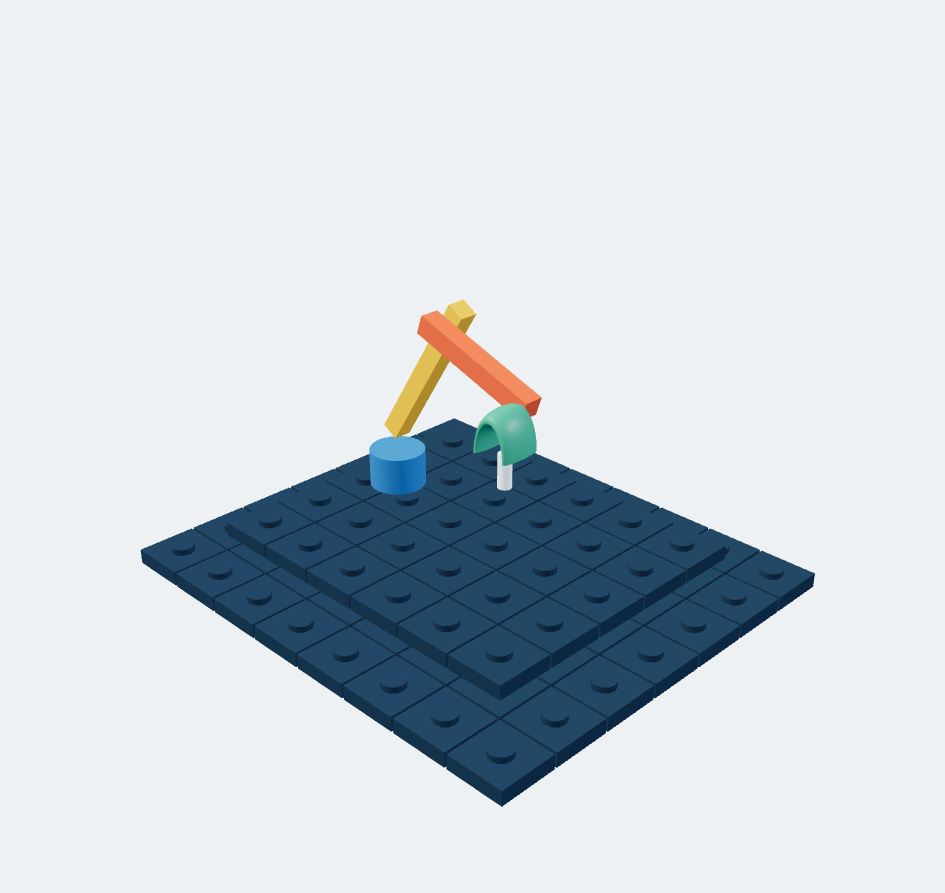
\includegraphics[width=.24\textwidth]{figures/hierarchy-expanded/exp-d1-arm-1-iso.png}
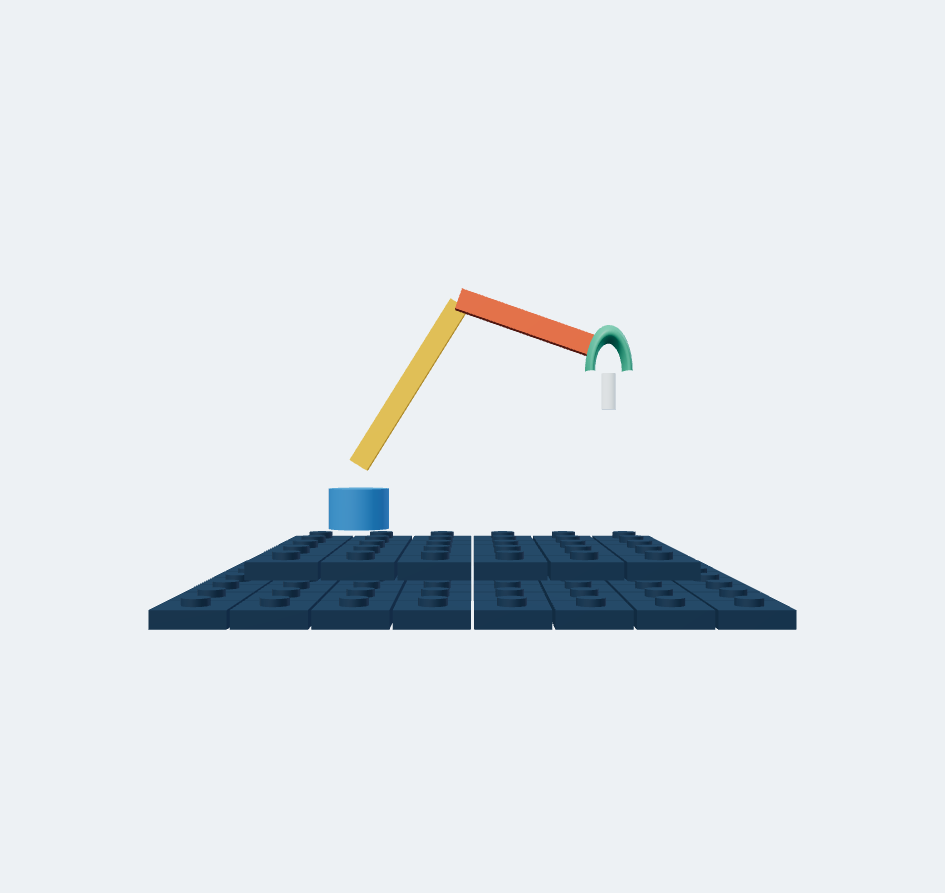
\includegraphics[width=.24\textwidth]{figures/hierarchy-expanded/exp-d1-arm-1-front.png}
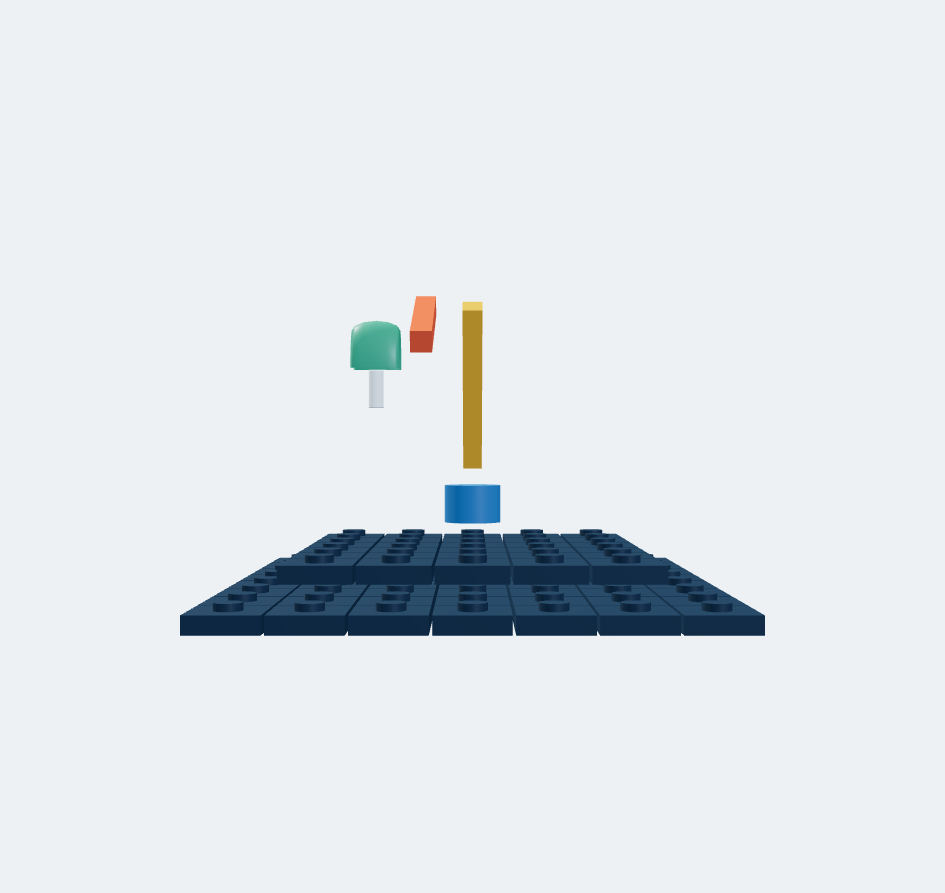
\includegraphics[width=.24\textwidth]{figures/hierarchy-expanded/exp-d1-arm-1-side.png}
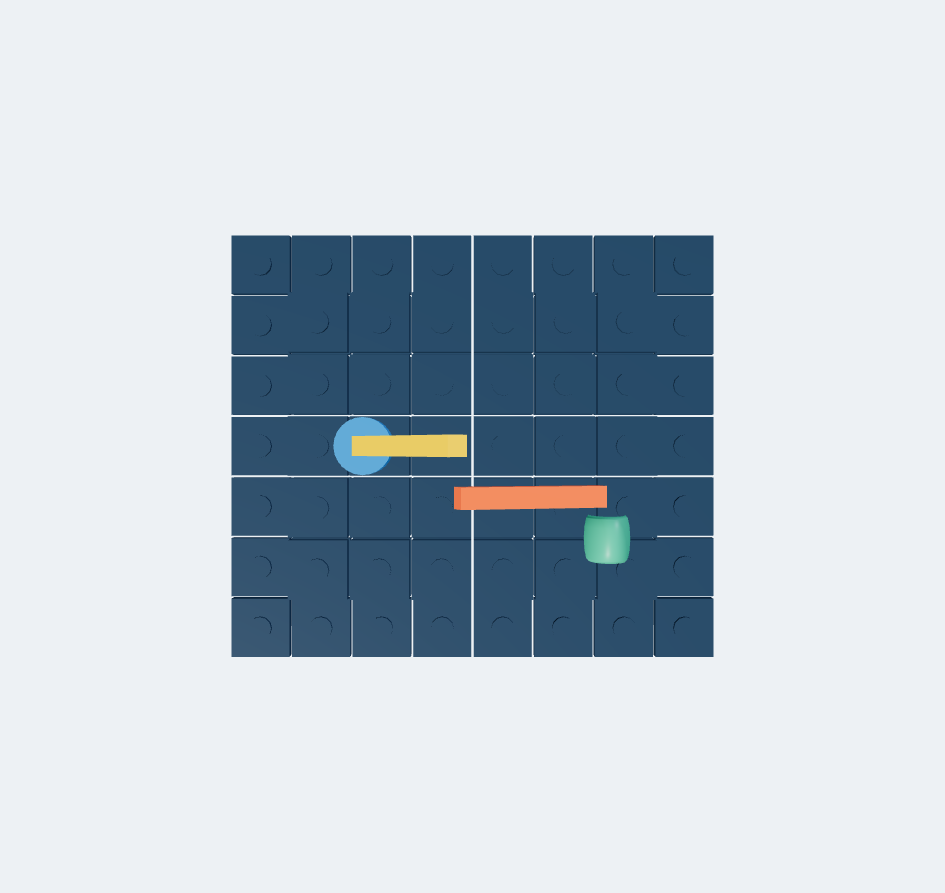
\includegraphics[width=.24\textwidth]{figures/hierarchy-expanded/exp-d1-arm-1-top.png}
\end{center}
\noindent All 48 families share this source. Full inputs and answers appear in the companion question bank.
\begin{center}\tiny\begin{tabular}{rllll}\toprule No. & Family & Layer & Output & Evidence\\\midrule
1 & identify & atomic & single-choice & model-state \\
2 & count & atomic & single-choice & model-state \\
3 & color & atomic & single-choice & model-state \\
4 & position & atomic & single-choice & model-state \\
5 & joint-type & atomic & single-choice & model-state \\
6 & parent & atomic & single-choice & model-state \\
7 & anchor & atomic & single-choice & model-state \\
8 & degree & atomic & single-choice & model-state \\
9 & recolor & atomic & single-choice & model-state \\
10 & add & atomic & single-choice & model-state \\
11 & remove & atomic & single-choice & model-state \\
12 & replace & atomic & single-choice & model-state \\
13 & translate & atomic & single-choice & model-state \\
14 & rotate & atomic & single-choice & model-state \\
15 & next-module & atomic & single-choice & model-state \\
16 & inventory & atomic & single-choice & model-state \\
17 & boundary & atomic & single-choice & model-state \\
18 & no-op & atomic & single-choice & model-state \\
19 & prefix & metacognitive & single-choice & support-graph \\
20 & access & metacognitive & multiple-choice & Rapier \\
21 & counterfactual & metacognitive & single-choice & support-graph \\
22 & dynamic & metacognitive & single-choice & Rapier \\
23 & kinematic & metacognitive & multiple-choice & model-state \\
24 & diagnosis & metacognitive & multiple-choice & model-state \\
25 & information-gain & metacognitive & multiple-choice & finite-world \\
26 & abstention & metacognitive & single-choice & finite-world \\
27 & posterior & metacognitive & single-choice & finite-world \\
28 & pareto & metacognitive & multiple-choice & model-state \\
29 & assembly & procedural & actions & state-machine \\
30 & disassembly & procedural & actions & state-machine \\
31 & service-repair & procedural & actions & state-machine \\
32 & compound-edit & procedural & actions & state-machine \\
33 & multi-fault & integrative & actions & state-machine \\
34 & scheduling & integrative & schedule & resource-schedule \\
35 & policy & integrative & policy & finite-world \\
36 & local-frame & atomic & single-choice & model-state \\
37 & projection & atomic & single-choice & model-state \\
38 & relative-order & atomic & single-choice & model-state \\
39 & joint-axis & atomic & single-choice & model-state \\
40 & clearance-margin & metacognitive & single-choice & model-state \\
41 & load-moment & metacognitive & single-choice & model-state \\
42 & weighted-posterior & metacognitive & single-choice & finite-world \\
43 & expected-loss & metacognitive & single-choice & finite-world \\
44 & trace-threshold & metacognitive & single-choice & Rapier \\
45 & guarded-repair & procedural & actions & state-machine \\
46 & rollback & procedural & actions & state-machine \\
47 & resource-repair & integrative & actions & state-machine \\
48 & budget-policy & integrative & policy & finite-world \\
\bottomrule\end{tabular}\end{center}
\clearpage
\subsection{3. Two-link Sampling Arm (D1)}
101 visible parts; 6 modules; 5 joints. Representative-point motion 0.0098; rotation 0.0024 rad.
\begin{center}
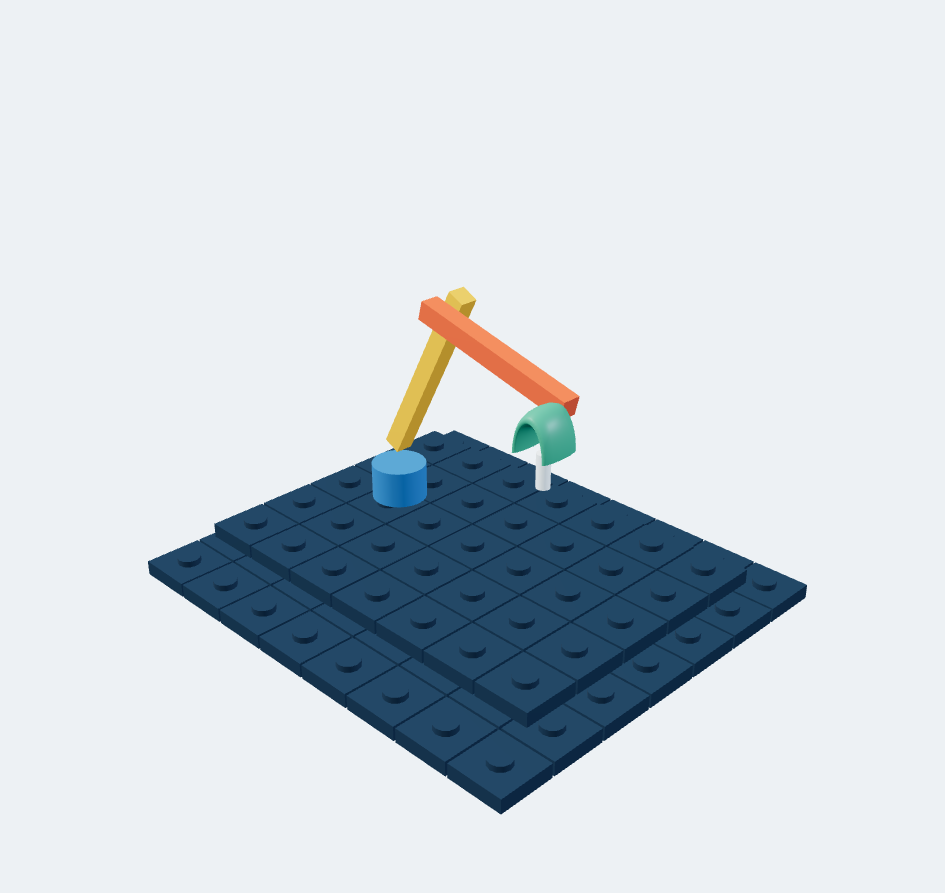
\includegraphics[width=.24\textwidth]{figures/hierarchy-expanded/exp-d1-arm-2-iso.png}
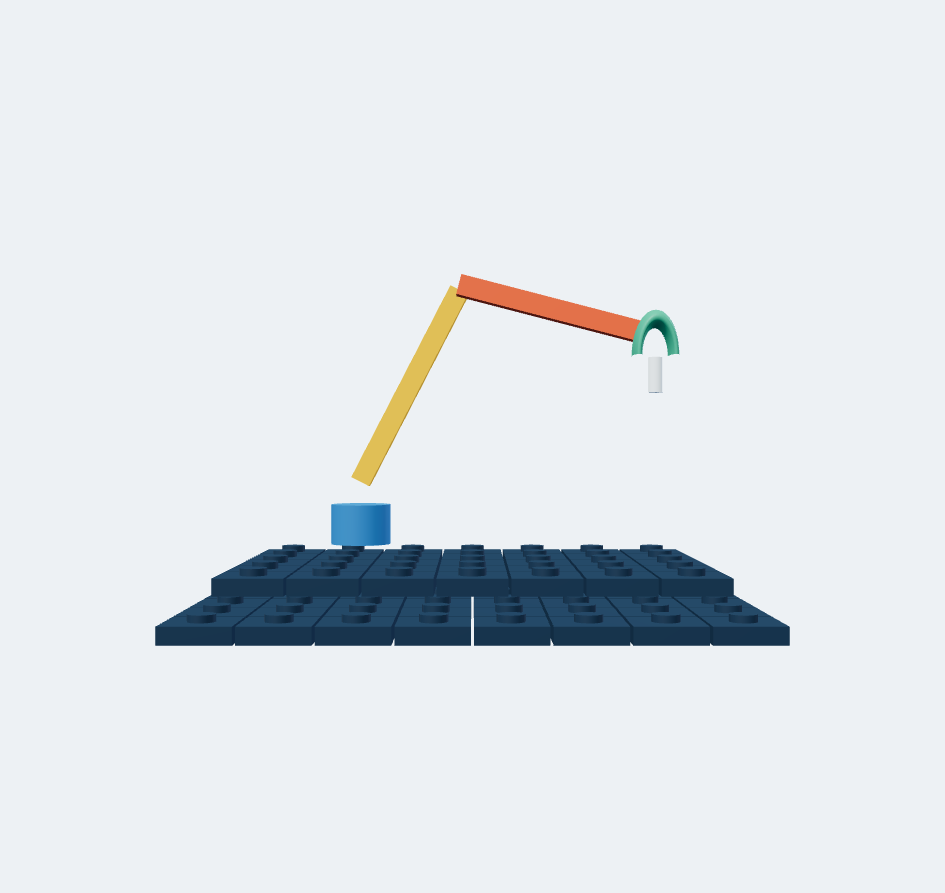
\includegraphics[width=.24\textwidth]{figures/hierarchy-expanded/exp-d1-arm-2-front.png}
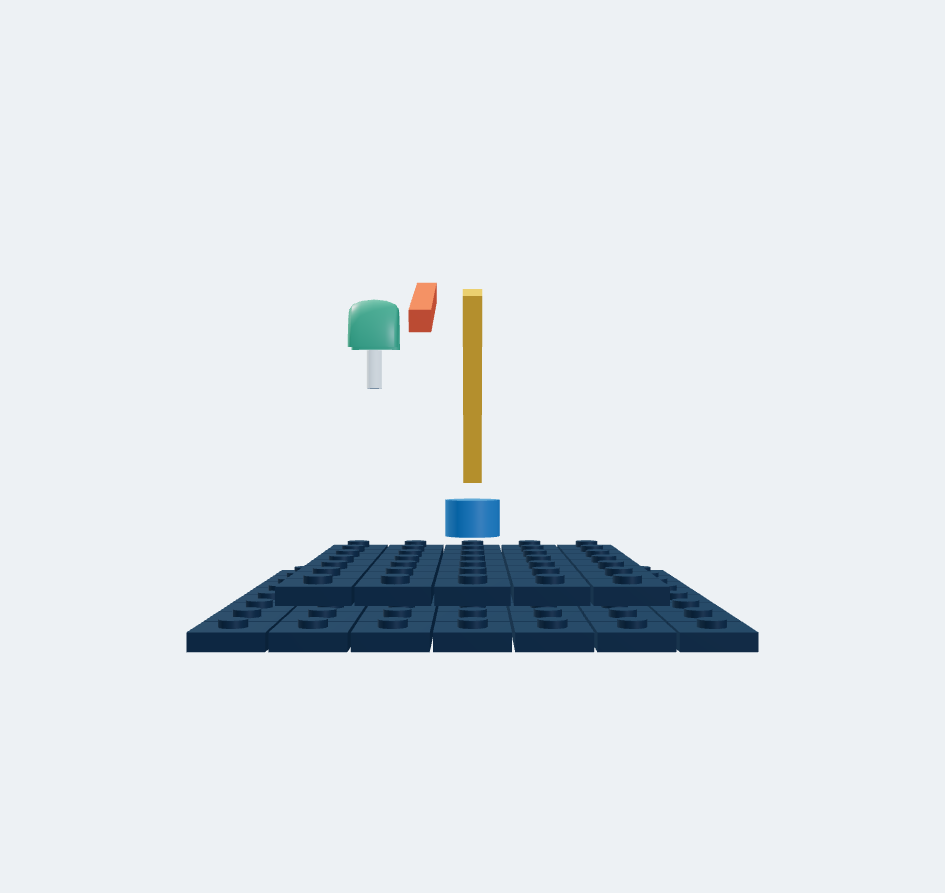
\includegraphics[width=.24\textwidth]{figures/hierarchy-expanded/exp-d1-arm-2-side.png}
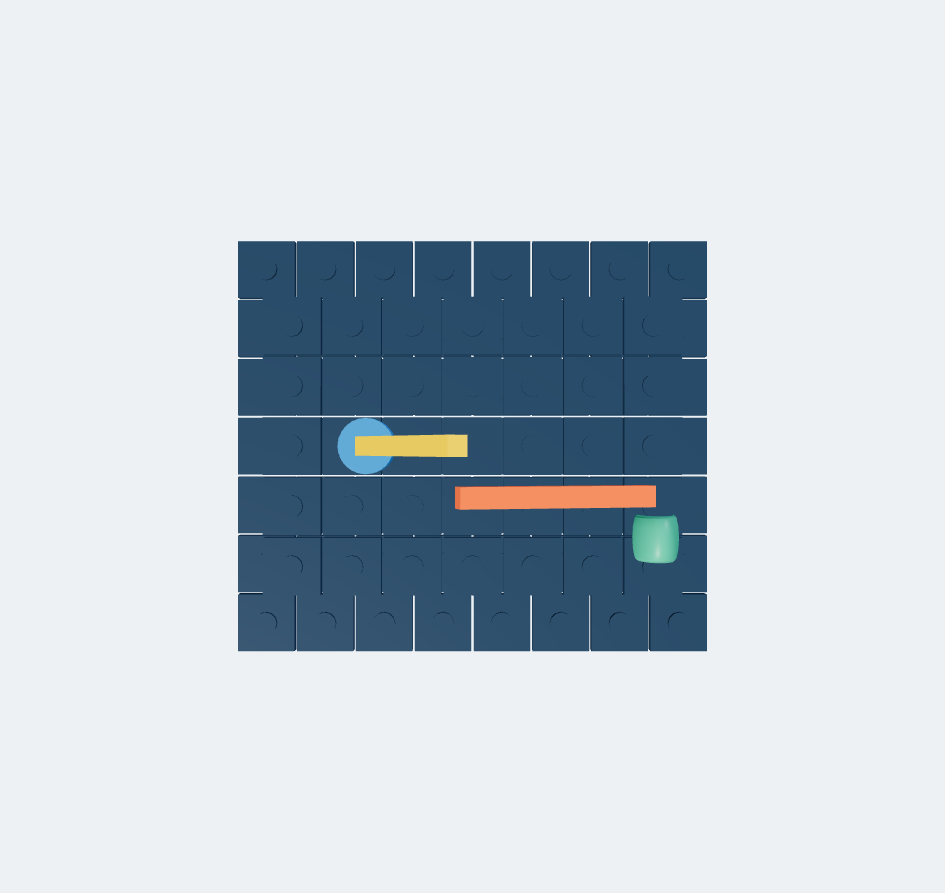
\includegraphics[width=.24\textwidth]{figures/hierarchy-expanded/exp-d1-arm-2-top.png}
\end{center}
\noindent All 48 families share this source. Full inputs and answers appear in the companion question bank.
\begin{center}\tiny\begin{tabular}{rllll}\toprule No. & Family & Layer & Output & Evidence\\\midrule
1 & identify & atomic & single-choice & model-state \\
2 & count & atomic & single-choice & model-state \\
3 & color & atomic & single-choice & model-state \\
4 & position & atomic & single-choice & model-state \\
5 & joint-type & atomic & single-choice & model-state \\
6 & parent & atomic & single-choice & model-state \\
7 & anchor & atomic & single-choice & model-state \\
8 & degree & atomic & single-choice & model-state \\
9 & recolor & atomic & single-choice & model-state \\
10 & add & atomic & single-choice & model-state \\
11 & remove & atomic & single-choice & model-state \\
12 & replace & atomic & single-choice & model-state \\
13 & translate & atomic & single-choice & model-state \\
14 & rotate & atomic & single-choice & model-state \\
15 & next-module & atomic & single-choice & model-state \\
16 & inventory & atomic & single-choice & model-state \\
17 & boundary & atomic & single-choice & model-state \\
18 & no-op & atomic & single-choice & model-state \\
19 & prefix & metacognitive & single-choice & support-graph \\
20 & access & metacognitive & multiple-choice & Rapier \\
21 & counterfactual & metacognitive & single-choice & support-graph \\
22 & dynamic & metacognitive & single-choice & Rapier \\
23 & kinematic & metacognitive & multiple-choice & model-state \\
24 & diagnosis & metacognitive & multiple-choice & model-state \\
25 & information-gain & metacognitive & multiple-choice & finite-world \\
26 & abstention & metacognitive & single-choice & finite-world \\
27 & posterior & metacognitive & single-choice & finite-world \\
28 & pareto & metacognitive & multiple-choice & model-state \\
29 & assembly & procedural & actions & state-machine \\
30 & disassembly & procedural & actions & state-machine \\
31 & service-repair & procedural & actions & state-machine \\
32 & compound-edit & procedural & actions & state-machine \\
33 & multi-fault & integrative & actions & state-machine \\
34 & scheduling & integrative & schedule & resource-schedule \\
35 & policy & integrative & policy & finite-world \\
36 & local-frame & atomic & single-choice & model-state \\
37 & projection & atomic & single-choice & model-state \\
38 & relative-order & atomic & single-choice & model-state \\
39 & joint-axis & atomic & single-choice & model-state \\
40 & clearance-margin & metacognitive & single-choice & model-state \\
41 & load-moment & metacognitive & single-choice & model-state \\
42 & weighted-posterior & metacognitive & single-choice & finite-world \\
43 & expected-loss & metacognitive & single-choice & finite-world \\
44 & trace-threshold & metacognitive & single-choice & Rapier \\
45 & guarded-repair & procedural & actions & state-machine \\
46 & rollback & procedural & actions & state-machine \\
47 & resource-repair & integrative & actions & state-machine \\
48 & budget-policy & integrative & policy & finite-world \\
\bottomrule\end{tabular}\end{center}
\clearpage
\subsection{4. Four-slot Sample Carousel (D1)}
96 visible parts; 8 modules; 7 joints. Representative-point motion 0.0000; rotation 0.0000 rad.
\begin{center}
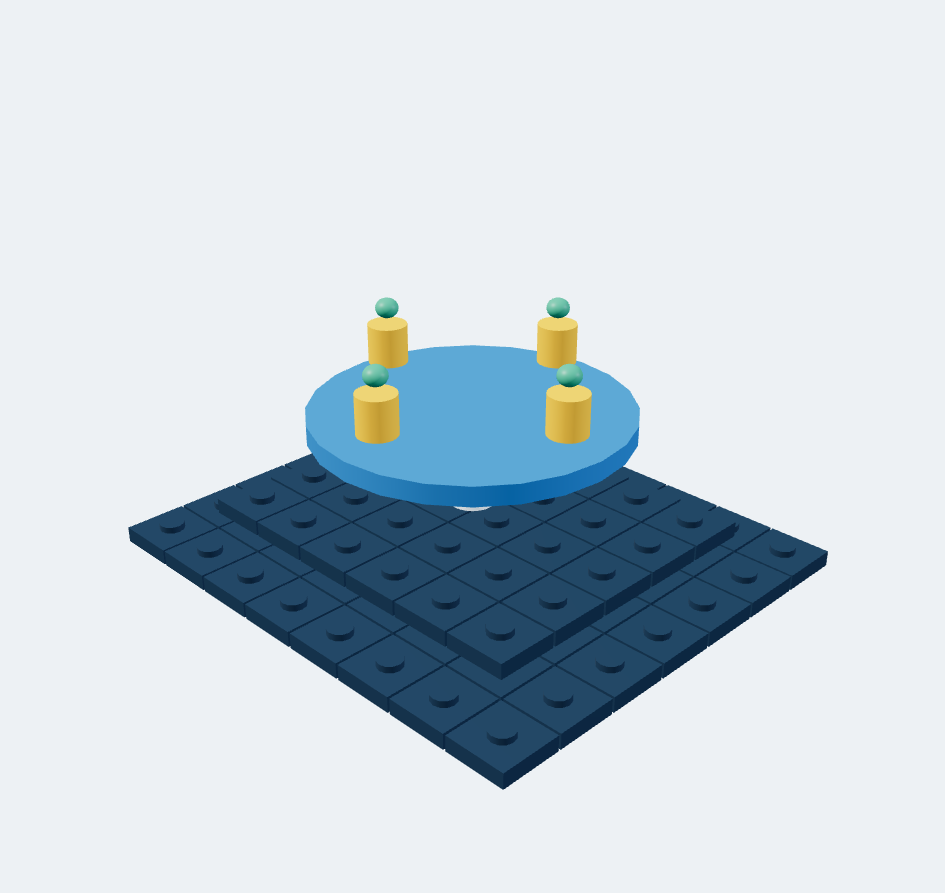
\includegraphics[width=.24\textwidth]{figures/hierarchy-expanded/exp-d1-carousel-1-iso.png}

\includegraphics[width=.24\textwidth]{figures/hierarchy-expanded/exp-d1-carousel-1-front.png}

\includegraphics[width=.24\textwidth]{figures/hierarchy-expanded/exp-d1-carousel-1-side.png}
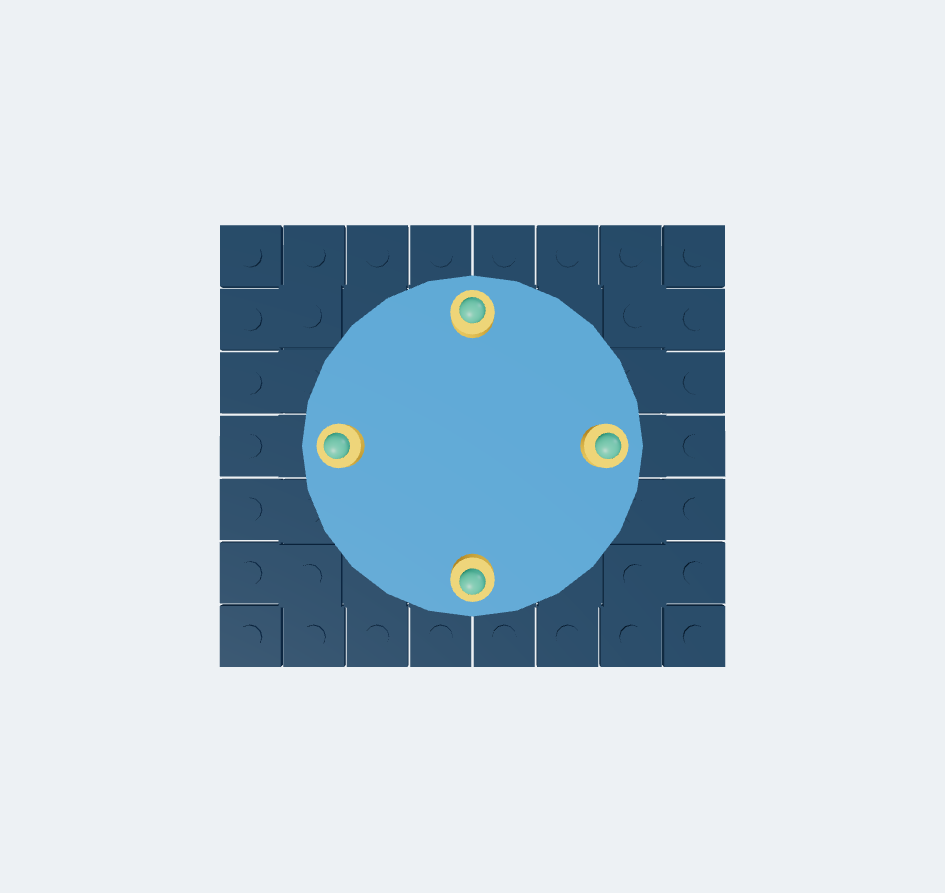
\includegraphics[width=.24\textwidth]{figures/hierarchy-expanded/exp-d1-carousel-1-top.png}
\end{center}
\noindent All 48 families share this source. Full inputs and answers appear in the companion question bank.
\begin{center}\tiny\begin{tabular}{rllll}\toprule No. & Family & Layer & Output & Evidence\\\midrule
1 & identify & atomic & single-choice & model-state \\
2 & count & atomic & single-choice & model-state \\
3 & color & atomic & single-choice & model-state \\
4 & position & atomic & single-choice & model-state \\
5 & joint-type & atomic & single-choice & model-state \\
6 & parent & atomic & single-choice & model-state \\
7 & anchor & atomic & single-choice & model-state \\
8 & degree & atomic & single-choice & model-state \\
9 & recolor & atomic & single-choice & model-state \\
10 & add & atomic & single-choice & model-state \\
11 & remove & atomic & single-choice & model-state \\
12 & replace & atomic & single-choice & model-state \\
13 & translate & atomic & single-choice & model-state \\
14 & rotate & atomic & single-choice & model-state \\
15 & next-module & atomic & single-choice & model-state \\
16 & inventory & atomic & single-choice & model-state \\
17 & boundary & atomic & single-choice & model-state \\
18 & no-op & atomic & single-choice & model-state \\
19 & prefix & metacognitive & single-choice & support-graph \\
20 & access & metacognitive & multiple-choice & Rapier \\
21 & counterfactual & metacognitive & single-choice & support-graph \\
22 & dynamic & metacognitive & single-choice & Rapier \\
23 & kinematic & metacognitive & multiple-choice & model-state \\
24 & diagnosis & metacognitive & multiple-choice & model-state \\
25 & information-gain & metacognitive & multiple-choice & finite-world \\
26 & abstention & metacognitive & single-choice & finite-world \\
27 & posterior & metacognitive & single-choice & finite-world \\
28 & pareto & metacognitive & multiple-choice & model-state \\
29 & assembly & procedural & actions & state-machine \\
30 & disassembly & procedural & actions & state-machine \\
31 & service-repair & procedural & actions & state-machine \\
32 & compound-edit & procedural & actions & state-machine \\
33 & multi-fault & integrative & actions & state-machine \\
34 & scheduling & integrative & schedule & resource-schedule \\
35 & policy & integrative & policy & finite-world \\
36 & local-frame & atomic & single-choice & model-state \\
37 & projection & atomic & single-choice & model-state \\
38 & relative-order & atomic & single-choice & model-state \\
39 & joint-axis & atomic & single-choice & model-state \\
40 & clearance-margin & metacognitive & single-choice & model-state \\
41 & load-moment & metacognitive & single-choice & model-state \\
42 & weighted-posterior & metacognitive & single-choice & finite-world \\
43 & expected-loss & metacognitive & single-choice & finite-world \\
44 & trace-threshold & metacognitive & single-choice & Rapier \\
45 & guarded-repair & procedural & actions & state-machine \\
46 & rollback & procedural & actions & state-machine \\
47 & resource-repair & integrative & actions & state-machine \\
48 & budget-policy & integrative & policy & finite-world \\
\bottomrule\end{tabular}\end{center}
\clearpage
\subsection{5. Six-slot Tube Carousel (D1)}
105 visible parts; 10 modules; 9 joints. Representative-point motion 0.0000; rotation 0.0000 rad.
\begin{center}
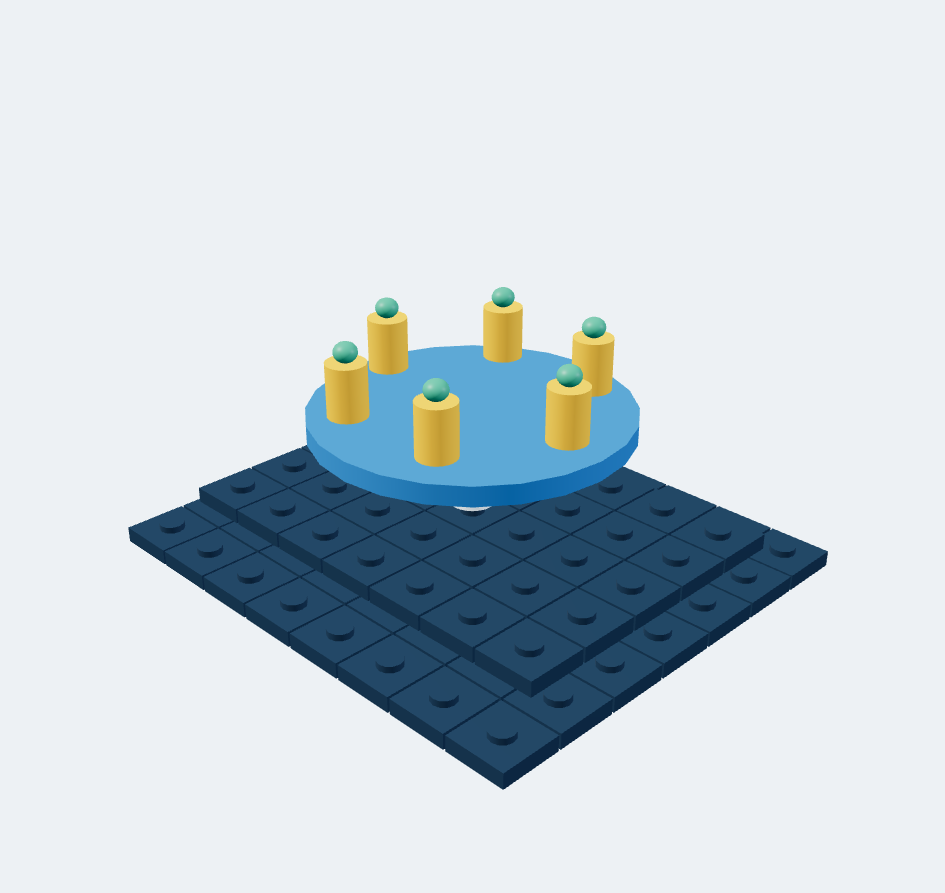
\includegraphics[width=.24\textwidth]{figures/hierarchy-expanded/exp-d1-carousel-2-iso.png}

\includegraphics[width=.24\textwidth]{figures/hierarchy-expanded/exp-d1-carousel-2-front.png}

\includegraphics[width=.24\textwidth]{figures/hierarchy-expanded/exp-d1-carousel-2-side.png}
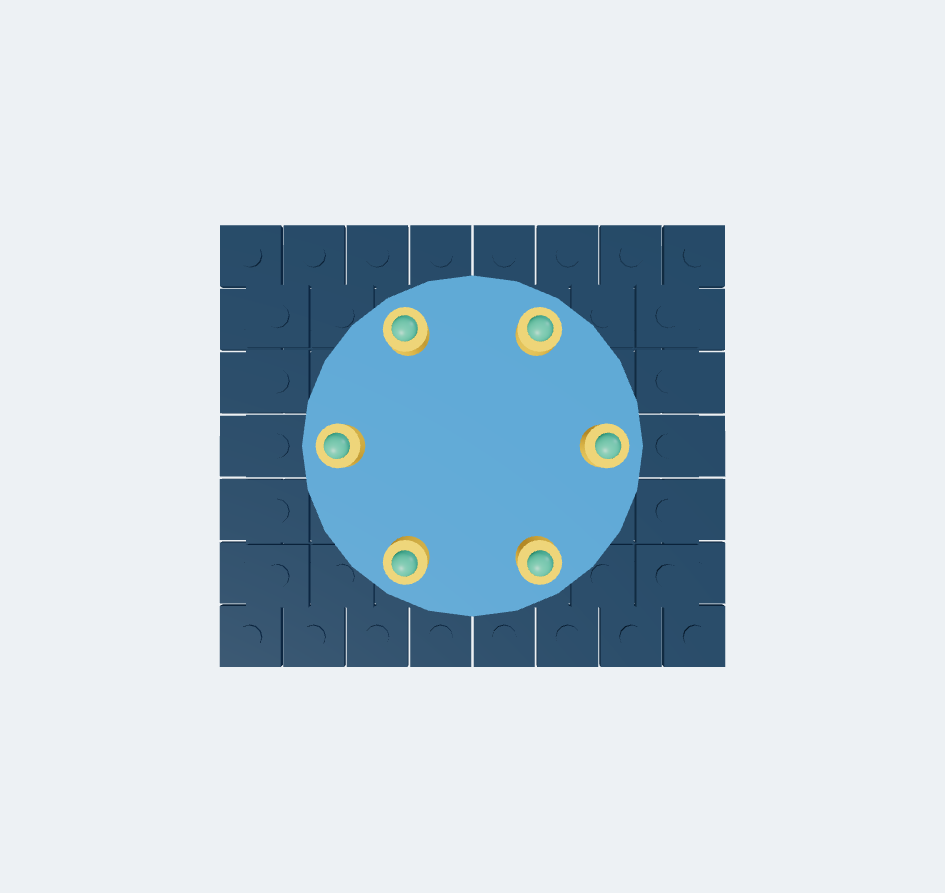
\includegraphics[width=.24\textwidth]{figures/hierarchy-expanded/exp-d1-carousel-2-top.png}
\end{center}
\noindent All 48 families share this source. Full inputs and answers appear in the companion question bank.
\begin{center}\tiny\begin{tabular}{rllll}\toprule No. & Family & Layer & Output & Evidence\\\midrule
1 & identify & atomic & single-choice & model-state \\
2 & count & atomic & single-choice & model-state \\
3 & color & atomic & single-choice & model-state \\
4 & position & atomic & single-choice & model-state \\
5 & joint-type & atomic & single-choice & model-state \\
6 & parent & atomic & single-choice & model-state \\
7 & anchor & atomic & single-choice & model-state \\
8 & degree & atomic & single-choice & model-state \\
9 & recolor & atomic & single-choice & model-state \\
10 & add & atomic & single-choice & model-state \\
11 & remove & atomic & single-choice & model-state \\
12 & replace & atomic & single-choice & model-state \\
13 & translate & atomic & single-choice & model-state \\
14 & rotate & atomic & single-choice & model-state \\
15 & next-module & atomic & single-choice & model-state \\
16 & inventory & atomic & single-choice & model-state \\
17 & boundary & atomic & single-choice & model-state \\
18 & no-op & atomic & single-choice & model-state \\
19 & prefix & metacognitive & single-choice & support-graph \\
20 & access & metacognitive & multiple-choice & Rapier \\
21 & counterfactual & metacognitive & single-choice & support-graph \\
22 & dynamic & metacognitive & single-choice & Rapier \\
23 & kinematic & metacognitive & multiple-choice & model-state \\
24 & diagnosis & metacognitive & multiple-choice & model-state \\
25 & information-gain & metacognitive & multiple-choice & finite-world \\
26 & abstention & metacognitive & single-choice & finite-world \\
27 & posterior & metacognitive & single-choice & finite-world \\
28 & pareto & metacognitive & multiple-choice & model-state \\
29 & assembly & procedural & actions & state-machine \\
30 & disassembly & procedural & actions & state-machine \\
31 & service-repair & procedural & actions & state-machine \\
32 & compound-edit & procedural & actions & state-machine \\
33 & multi-fault & integrative & actions & state-machine \\
34 & scheduling & integrative & schedule & resource-schedule \\
35 & policy & integrative & policy & finite-world \\
36 & local-frame & atomic & single-choice & model-state \\
37 & projection & atomic & single-choice & model-state \\
38 & relative-order & atomic & single-choice & model-state \\
39 & joint-axis & atomic & single-choice & model-state \\
40 & clearance-margin & metacognitive & single-choice & model-state \\
41 & load-moment & metacognitive & single-choice & model-state \\
42 & weighted-posterior & metacognitive & single-choice & finite-world \\
43 & expected-loss & metacognitive & single-choice & finite-world \\
44 & trace-threshold & metacognitive & single-choice & Rapier \\
45 & guarded-repair & procedural & actions & state-machine \\
46 & rollback & procedural & actions & state-machine \\
47 & resource-repair & integrative & actions & state-machine \\
48 & budget-policy & integrative & policy & finite-world \\
\bottomrule\end{tabular}\end{center}
\clearpage
\subsection{6. Tilting Cradle (D1)}
100 visible parts; 5 modules; 4 joints. Representative-point motion 0.0000; rotation 0.0000 rad.
\begin{center}
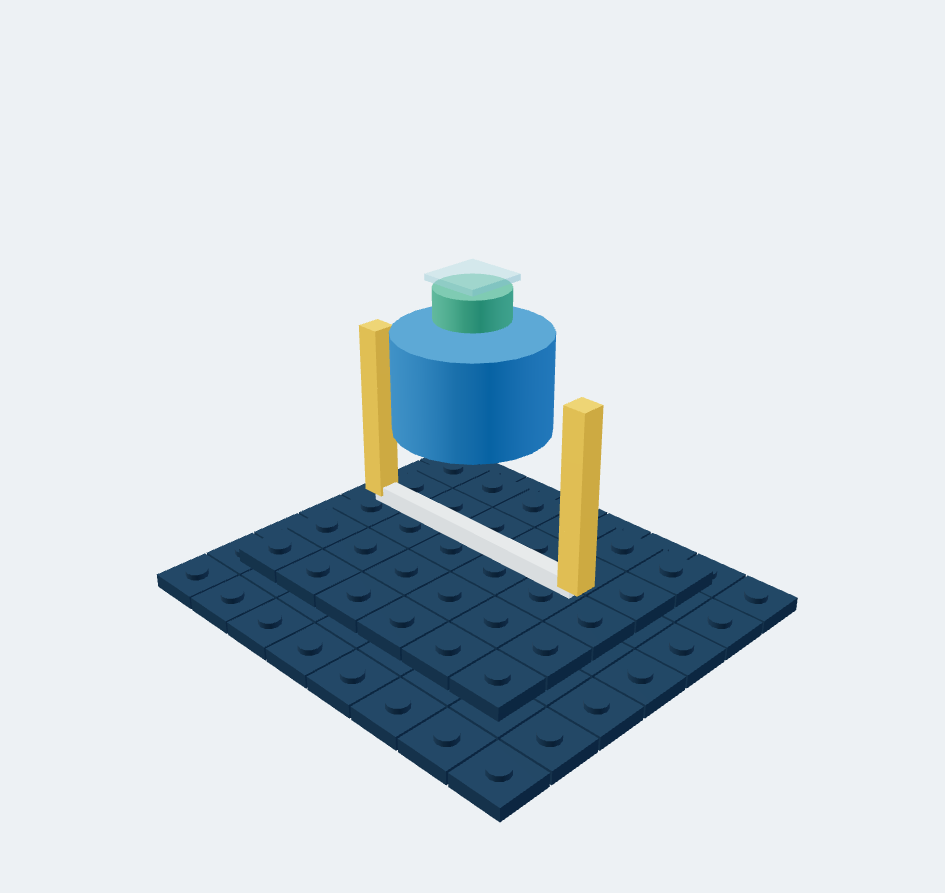
\includegraphics[width=.24\textwidth]{figures/hierarchy-expanded/exp-d1-cradle-1-iso.png}
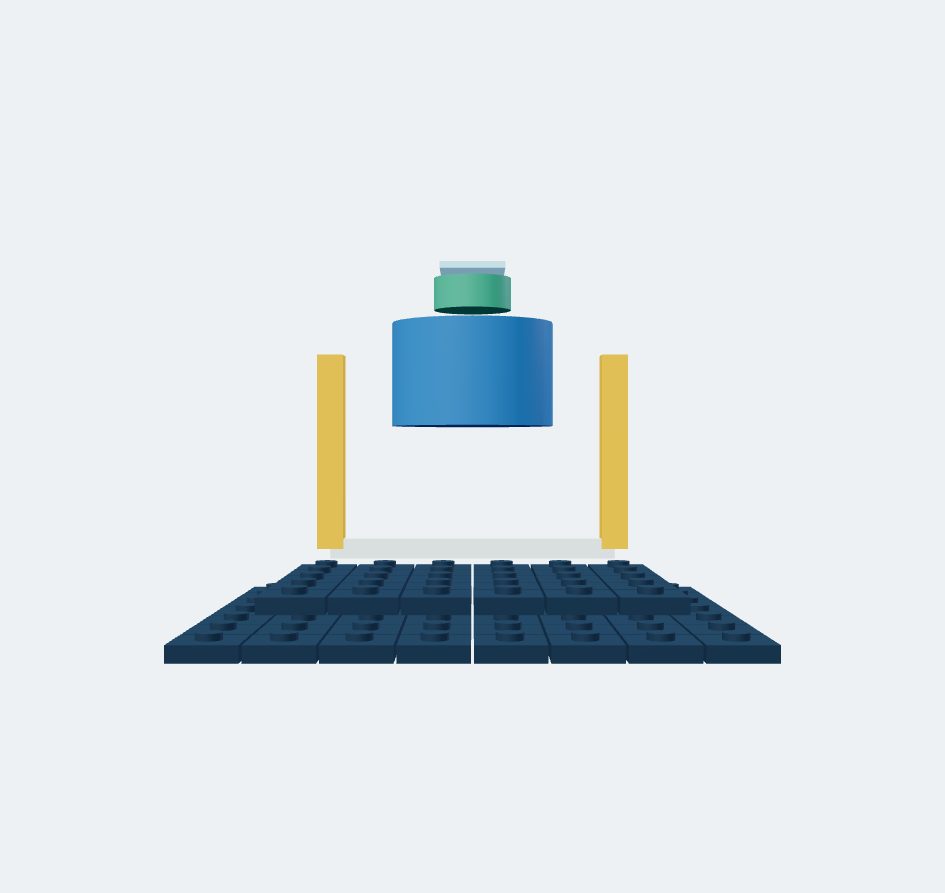
\includegraphics[width=.24\textwidth]{figures/hierarchy-expanded/exp-d1-cradle-1-front.png}
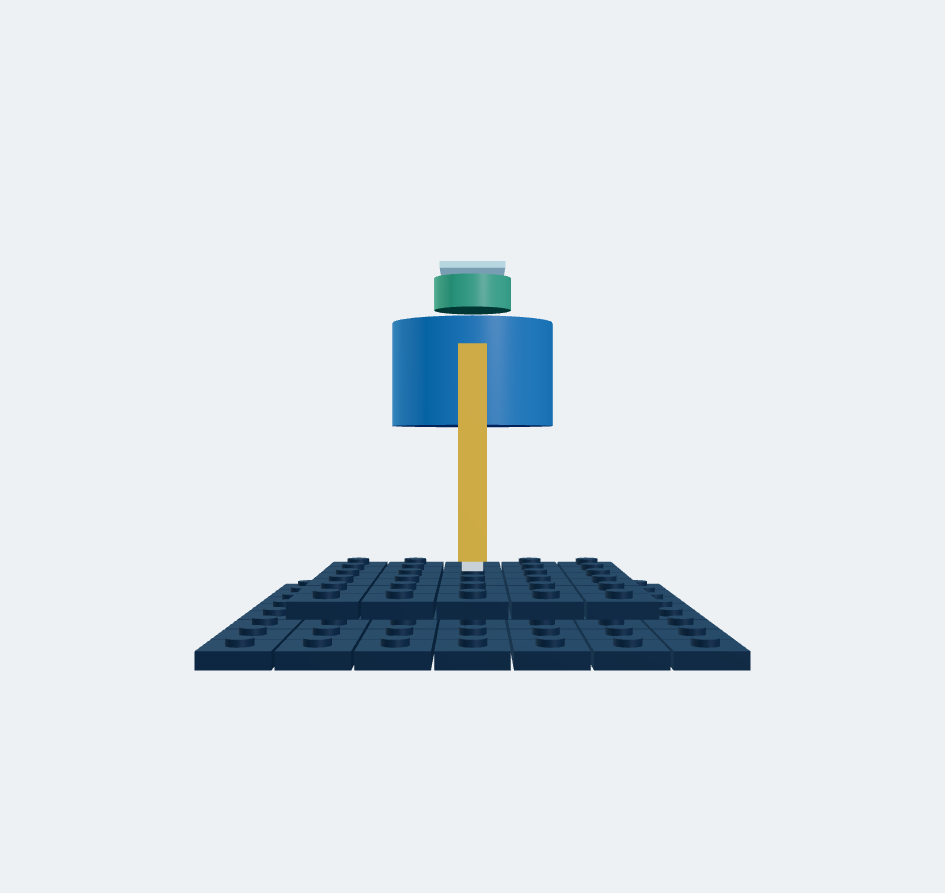
\includegraphics[width=.24\textwidth]{figures/hierarchy-expanded/exp-d1-cradle-1-side.png}
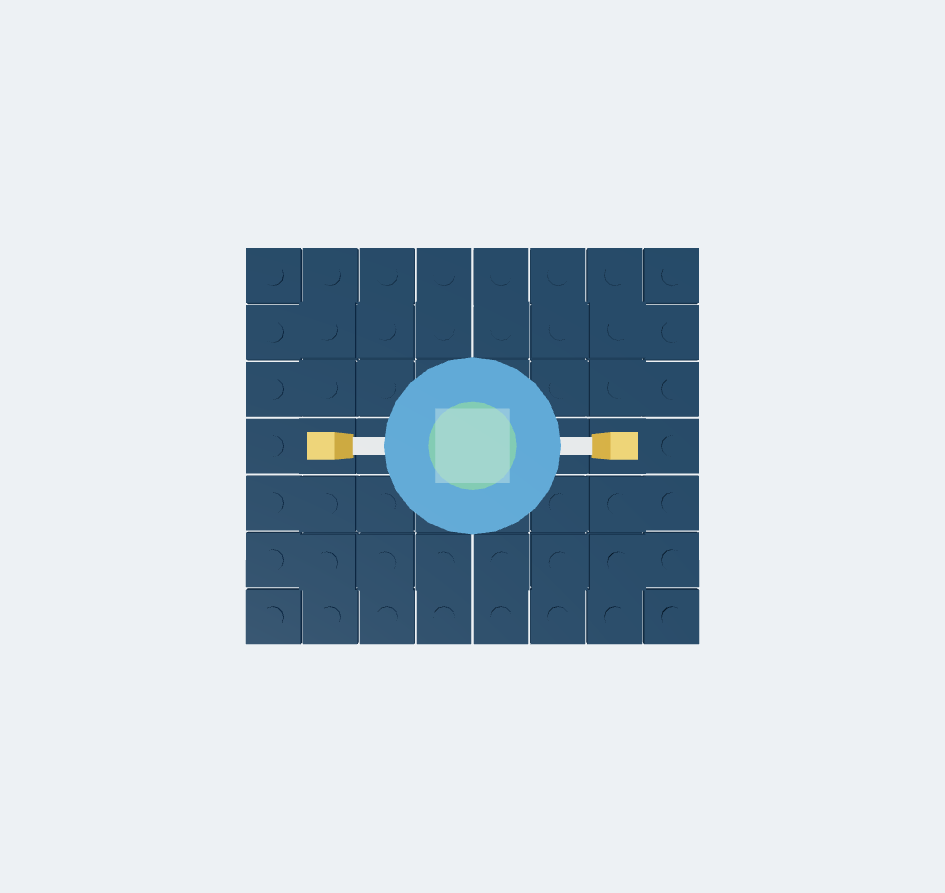
\includegraphics[width=.24\textwidth]{figures/hierarchy-expanded/exp-d1-cradle-1-top.png}
\end{center}
\noindent All 48 families share this source. Full inputs and answers appear in the companion question bank.
\begin{center}\tiny\begin{tabular}{rllll}\toprule No. & Family & Layer & Output & Evidence\\\midrule
1 & identify & atomic & single-choice & model-state \\
2 & count & atomic & single-choice & model-state \\
3 & color & atomic & single-choice & model-state \\
4 & position & atomic & single-choice & model-state \\
5 & joint-type & atomic & single-choice & model-state \\
6 & parent & atomic & single-choice & model-state \\
7 & anchor & atomic & single-choice & model-state \\
8 & degree & atomic & single-choice & model-state \\
9 & recolor & atomic & single-choice & model-state \\
10 & add & atomic & single-choice & model-state \\
11 & remove & atomic & single-choice & model-state \\
12 & replace & atomic & single-choice & model-state \\
13 & translate & atomic & single-choice & model-state \\
14 & rotate & atomic & single-choice & model-state \\
15 & next-module & atomic & single-choice & model-state \\
16 & inventory & atomic & single-choice & model-state \\
17 & boundary & atomic & single-choice & model-state \\
18 & no-op & atomic & single-choice & model-state \\
19 & prefix & metacognitive & single-choice & support-graph \\
20 & access & metacognitive & multiple-choice & Rapier \\
21 & counterfactual & metacognitive & single-choice & support-graph \\
22 & dynamic & metacognitive & single-choice & Rapier \\
23 & kinematic & metacognitive & multiple-choice & model-state \\
24 & diagnosis & metacognitive & multiple-choice & model-state \\
25 & information-gain & metacognitive & multiple-choice & finite-world \\
26 & abstention & metacognitive & single-choice & finite-world \\
27 & posterior & metacognitive & single-choice & finite-world \\
28 & pareto & metacognitive & multiple-choice & model-state \\
29 & assembly & procedural & actions & state-machine \\
30 & disassembly & procedural & actions & state-machine \\
31 & service-repair & procedural & actions & state-machine \\
32 & compound-edit & procedural & actions & state-machine \\
33 & multi-fault & integrative & actions & state-machine \\
34 & scheduling & integrative & schedule & resource-schedule \\
35 & policy & integrative & policy & finite-world \\
36 & local-frame & atomic & single-choice & model-state \\
37 & projection & atomic & single-choice & model-state \\
38 & relative-order & atomic & single-choice & model-state \\
39 & joint-axis & atomic & single-choice & model-state \\
40 & clearance-margin & metacognitive & single-choice & model-state \\
41 & load-moment & metacognitive & single-choice & model-state \\
42 & weighted-posterior & metacognitive & single-choice & finite-world \\
43 & expected-loss & metacognitive & single-choice & finite-world \\
44 & trace-threshold & metacognitive & single-choice & Rapier \\
45 & guarded-repair & procedural & actions & state-machine \\
46 & rollback & procedural & actions & state-machine \\
47 & resource-repair & integrative & actions & state-machine \\
48 & budget-policy & integrative & policy & finite-world \\
\bottomrule\end{tabular}\end{center}
\clearpage
\subsection{7. Two-axis Optical Cradle (D1)}
105 visible parts; 5 modules; 4 joints. Representative-point motion 0.0000; rotation 0.0000 rad.
\begin{center}
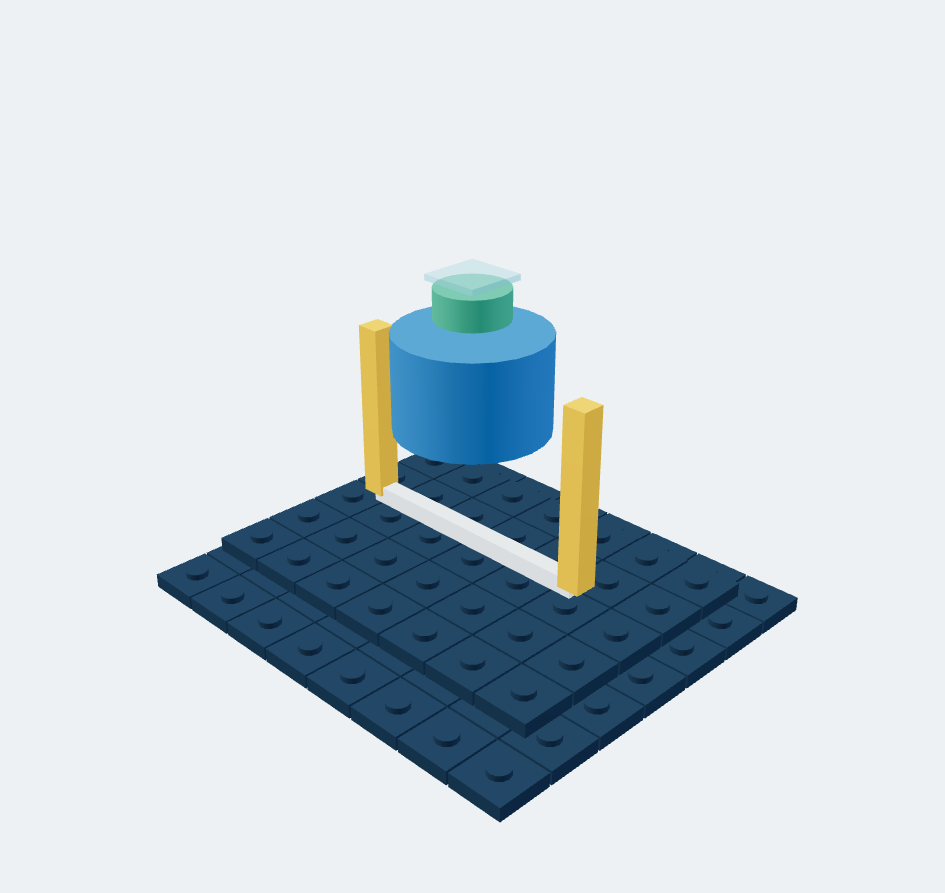
\includegraphics[width=.24\textwidth]{figures/hierarchy-expanded/exp-d1-cradle-2-iso.png}
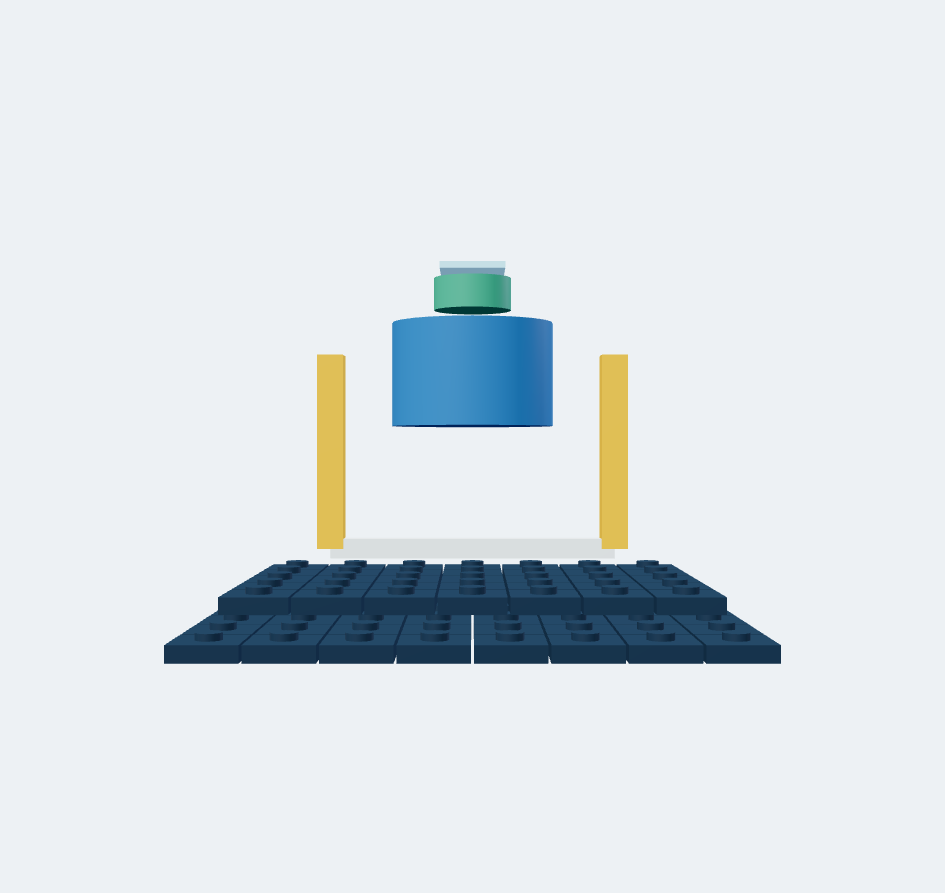
\includegraphics[width=.24\textwidth]{figures/hierarchy-expanded/exp-d1-cradle-2-front.png}
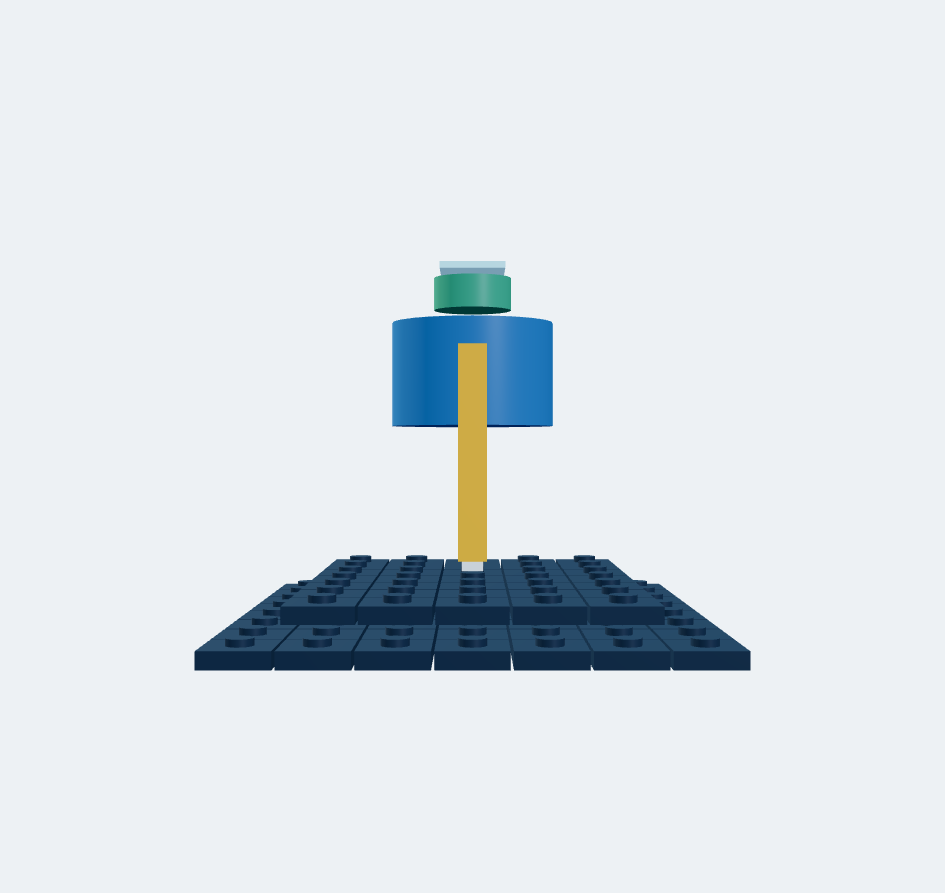
\includegraphics[width=.24\textwidth]{figures/hierarchy-expanded/exp-d1-cradle-2-side.png}
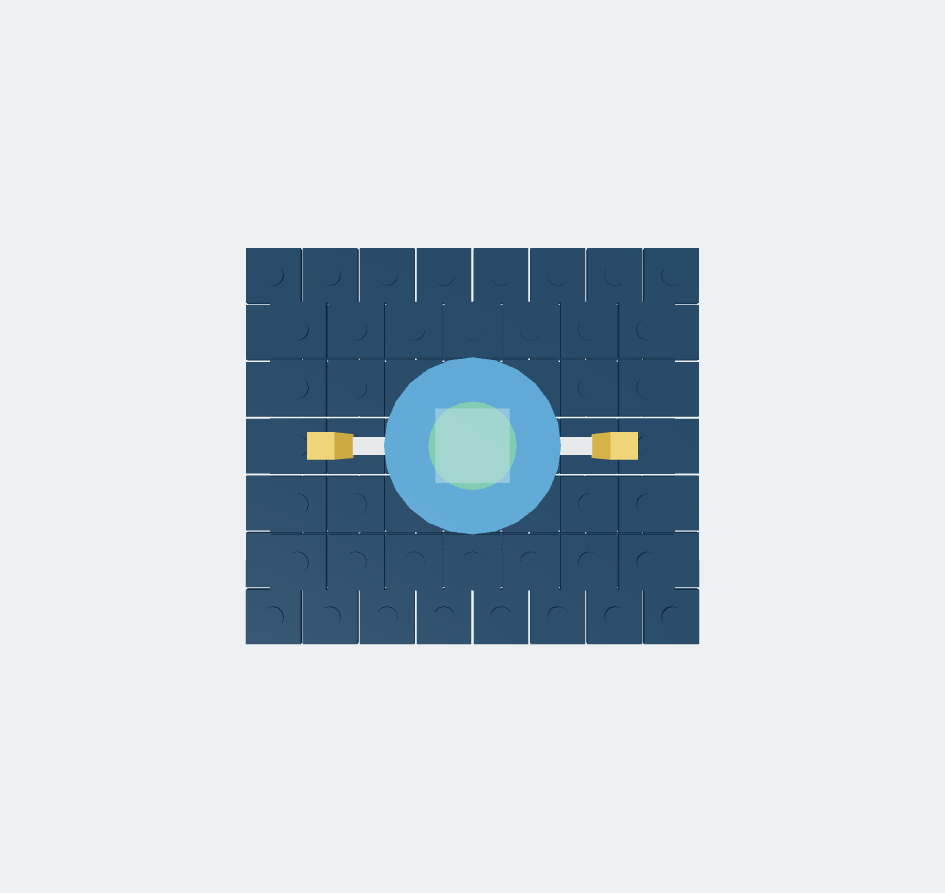
\includegraphics[width=.24\textwidth]{figures/hierarchy-expanded/exp-d1-cradle-2-top.png}
\end{center}
\noindent All 48 families share this source. Full inputs and answers appear in the companion question bank.
\begin{center}\tiny\begin{tabular}{rllll}\toprule No. & Family & Layer & Output & Evidence\\\midrule
1 & identify & atomic & single-choice & model-state \\
2 & count & atomic & single-choice & model-state \\
3 & color & atomic & single-choice & model-state \\
4 & position & atomic & single-choice & model-state \\
5 & joint-type & atomic & single-choice & model-state \\
6 & parent & atomic & single-choice & model-state \\
7 & anchor & atomic & single-choice & model-state \\
8 & degree & atomic & single-choice & model-state \\
9 & recolor & atomic & single-choice & model-state \\
10 & add & atomic & single-choice & model-state \\
11 & remove & atomic & single-choice & model-state \\
12 & replace & atomic & single-choice & model-state \\
13 & translate & atomic & single-choice & model-state \\
14 & rotate & atomic & single-choice & model-state \\
15 & next-module & atomic & single-choice & model-state \\
16 & inventory & atomic & single-choice & model-state \\
17 & boundary & atomic & single-choice & model-state \\
18 & no-op & atomic & single-choice & model-state \\
19 & prefix & metacognitive & single-choice & support-graph \\
20 & access & metacognitive & multiple-choice & Rapier \\
21 & counterfactual & metacognitive & single-choice & support-graph \\
22 & dynamic & metacognitive & single-choice & Rapier \\
23 & kinematic & metacognitive & multiple-choice & model-state \\
24 & diagnosis & metacognitive & multiple-choice & model-state \\
25 & information-gain & metacognitive & multiple-choice & finite-world \\
26 & abstention & metacognitive & single-choice & finite-world \\
27 & posterior & metacognitive & single-choice & finite-world \\
28 & pareto & metacognitive & multiple-choice & model-state \\
29 & assembly & procedural & actions & state-machine \\
30 & disassembly & procedural & actions & state-machine \\
31 & service-repair & procedural & actions & state-machine \\
32 & compound-edit & procedural & actions & state-machine \\
33 & multi-fault & integrative & actions & state-machine \\
34 & scheduling & integrative & schedule & resource-schedule \\
35 & policy & integrative & policy & finite-world \\
36 & local-frame & atomic & single-choice & model-state \\
37 & projection & atomic & single-choice & model-state \\
38 & relative-order & atomic & single-choice & model-state \\
39 & joint-axis & atomic & single-choice & model-state \\
40 & clearance-margin & metacognitive & single-choice & model-state \\
41 & load-moment & metacognitive & single-choice & model-state \\
42 & weighted-posterior & metacognitive & single-choice & finite-world \\
43 & expected-loss & metacognitive & single-choice & finite-world \\
44 & trace-threshold & metacognitive & single-choice & Rapier \\
45 & guarded-repair & procedural & actions & state-machine \\
46 & rollback & procedural & actions & state-machine \\
47 & resource-repair & integrative & actions & state-machine \\
48 & budget-policy & integrative & policy & finite-world \\
\bottomrule\end{tabular}\end{center}
\clearpage
\subsection{8. Horizontal Drum Stand (D1)}
95 visible parts; 3 modules; 2 joints. Representative-point motion 0.0000; rotation 0.0000 rad.
\begin{center}
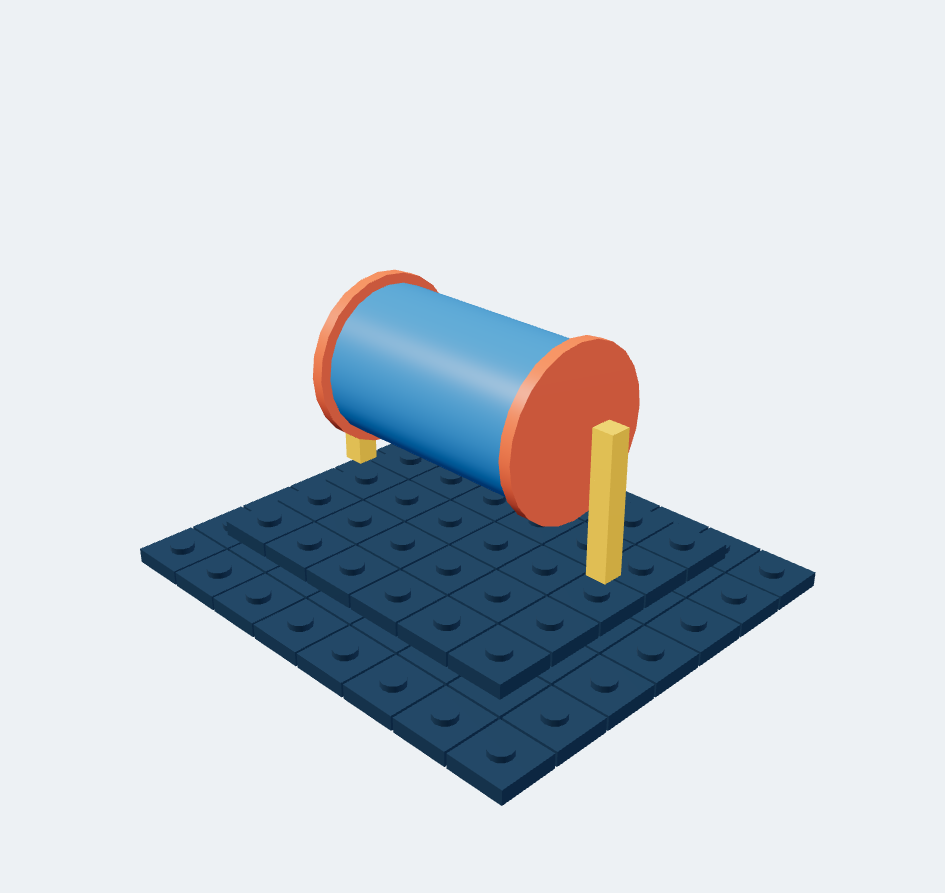
\includegraphics[width=.24\textwidth]{figures/hierarchy-expanded/exp-d1-drum-1-iso.png}
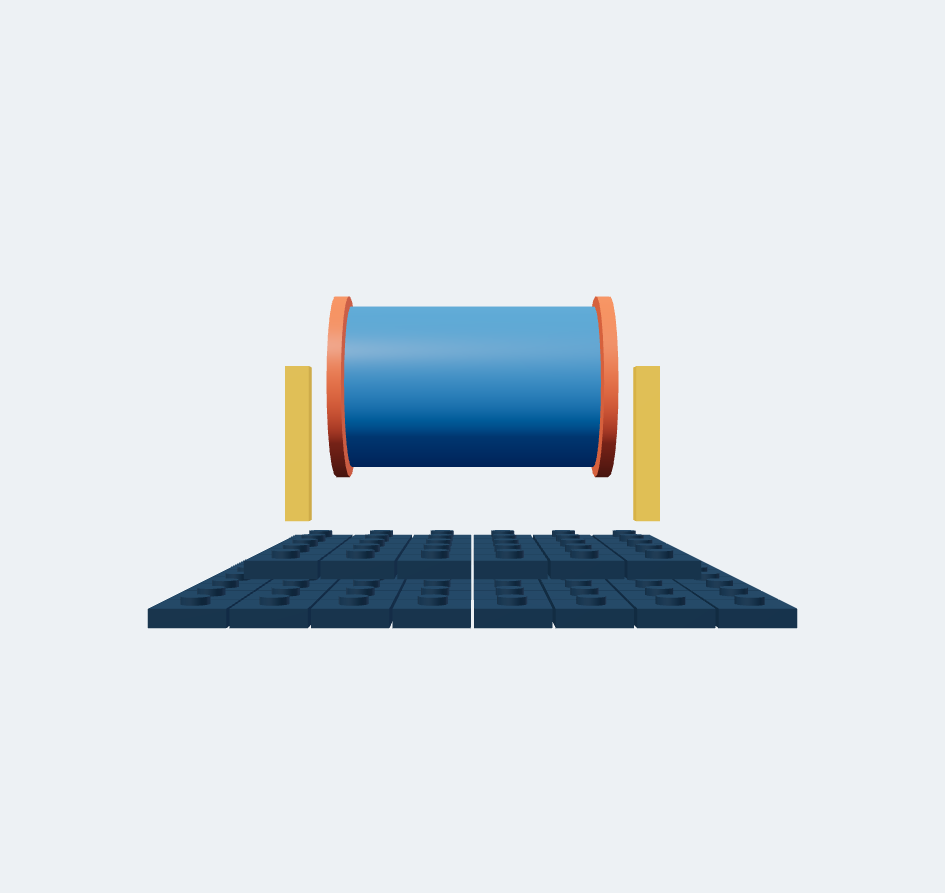
\includegraphics[width=.24\textwidth]{figures/hierarchy-expanded/exp-d1-drum-1-front.png}
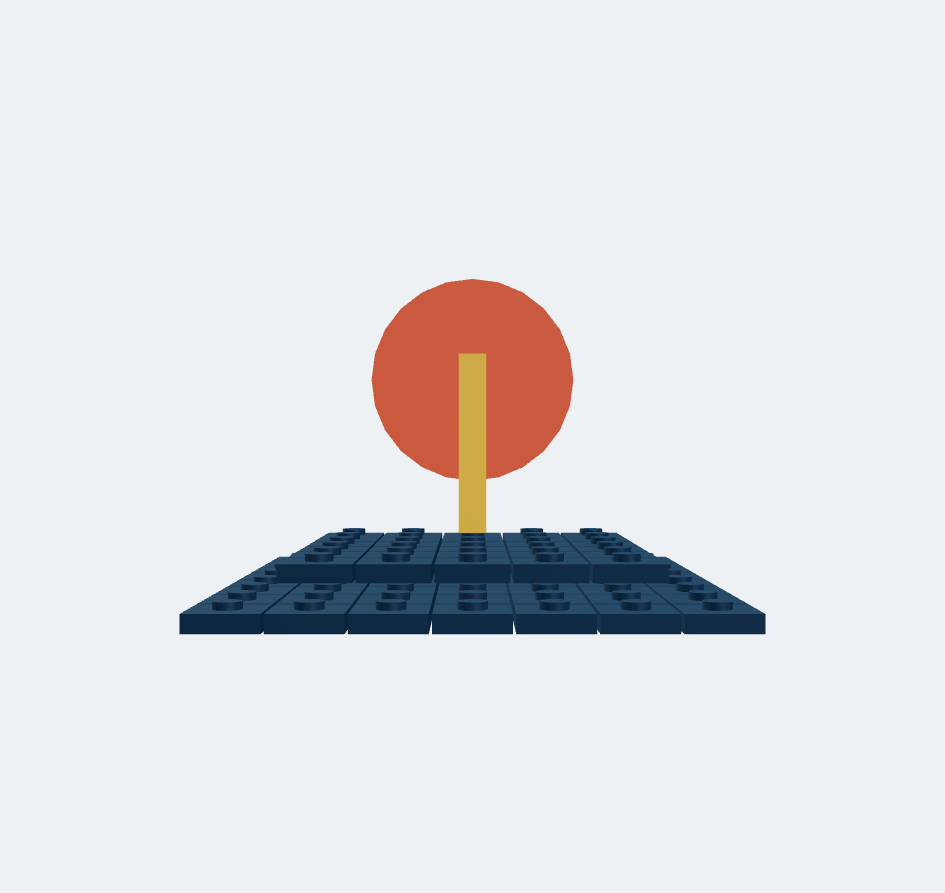
\includegraphics[width=.24\textwidth]{figures/hierarchy-expanded/exp-d1-drum-1-side.png}
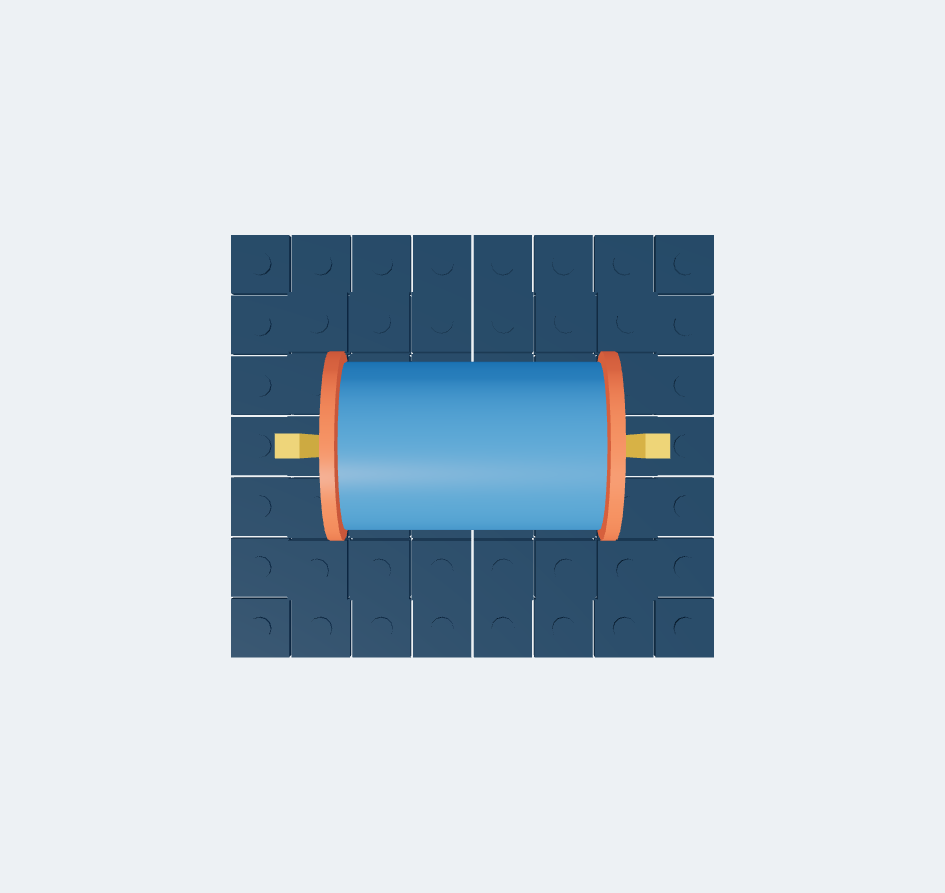
\includegraphics[width=.24\textwidth]{figures/hierarchy-expanded/exp-d1-drum-1-top.png}
\end{center}
\noindent All 48 families share this source. Full inputs and answers appear in the companion question bank.
\begin{center}\tiny\begin{tabular}{rllll}\toprule No. & Family & Layer & Output & Evidence\\\midrule
1 & identify & atomic & single-choice & model-state \\
2 & count & atomic & single-choice & model-state \\
3 & color & atomic & single-choice & model-state \\
4 & position & atomic & single-choice & model-state \\
5 & joint-type & atomic & single-choice & model-state \\
6 & parent & atomic & single-choice & model-state \\
7 & anchor & atomic & single-choice & model-state \\
8 & degree & atomic & single-choice & model-state \\
9 & recolor & atomic & single-choice & model-state \\
10 & add & atomic & single-choice & model-state \\
11 & remove & atomic & single-choice & model-state \\
12 & replace & atomic & single-choice & model-state \\
13 & translate & atomic & single-choice & model-state \\
14 & rotate & atomic & single-choice & model-state \\
15 & next-module & atomic & single-choice & model-state \\
16 & inventory & atomic & single-choice & model-state \\
17 & boundary & atomic & single-choice & model-state \\
18 & no-op & atomic & single-choice & model-state \\
19 & prefix & metacognitive & single-choice & support-graph \\
20 & access & metacognitive & multiple-choice & Rapier \\
21 & counterfactual & metacognitive & single-choice & support-graph \\
22 & dynamic & metacognitive & single-choice & Rapier \\
23 & kinematic & metacognitive & multiple-choice & model-state \\
24 & diagnosis & metacognitive & multiple-choice & model-state \\
25 & information-gain & metacognitive & multiple-choice & finite-world \\
26 & abstention & metacognitive & single-choice & finite-world \\
27 & posterior & metacognitive & single-choice & finite-world \\
28 & pareto & metacognitive & multiple-choice & model-state \\
29 & assembly & procedural & actions & state-machine \\
30 & disassembly & procedural & actions & state-machine \\
31 & service-repair & procedural & actions & state-machine \\
32 & compound-edit & procedural & actions & state-machine \\
33 & multi-fault & integrative & actions & state-machine \\
34 & scheduling & integrative & schedule & resource-schedule \\
35 & policy & integrative & policy & finite-world \\
36 & local-frame & atomic & single-choice & model-state \\
37 & projection & atomic & single-choice & model-state \\
38 & relative-order & atomic & single-choice & model-state \\
39 & joint-axis & atomic & single-choice & model-state \\
40 & clearance-margin & metacognitive & single-choice & model-state \\
41 & load-moment & metacognitive & single-choice & model-state \\
42 & weighted-posterior & metacognitive & single-choice & finite-world \\
43 & expected-loss & metacognitive & single-choice & finite-world \\
44 & trace-threshold & metacognitive & single-choice & Rapier \\
45 & guarded-repair & procedural & actions & state-machine \\
46 & rollback & procedural & actions & state-machine \\
47 & resource-repair & integrative & actions & state-machine \\
48 & budget-policy & integrative & policy & finite-world \\
\bottomrule\end{tabular}\end{center}
\clearpage
\subsection{9. Twin-drum Indexer (D1)}
103 visible parts; 4 modules; 3 joints. Representative-point motion 0.0000; rotation 0.0000 rad.
\begin{center}
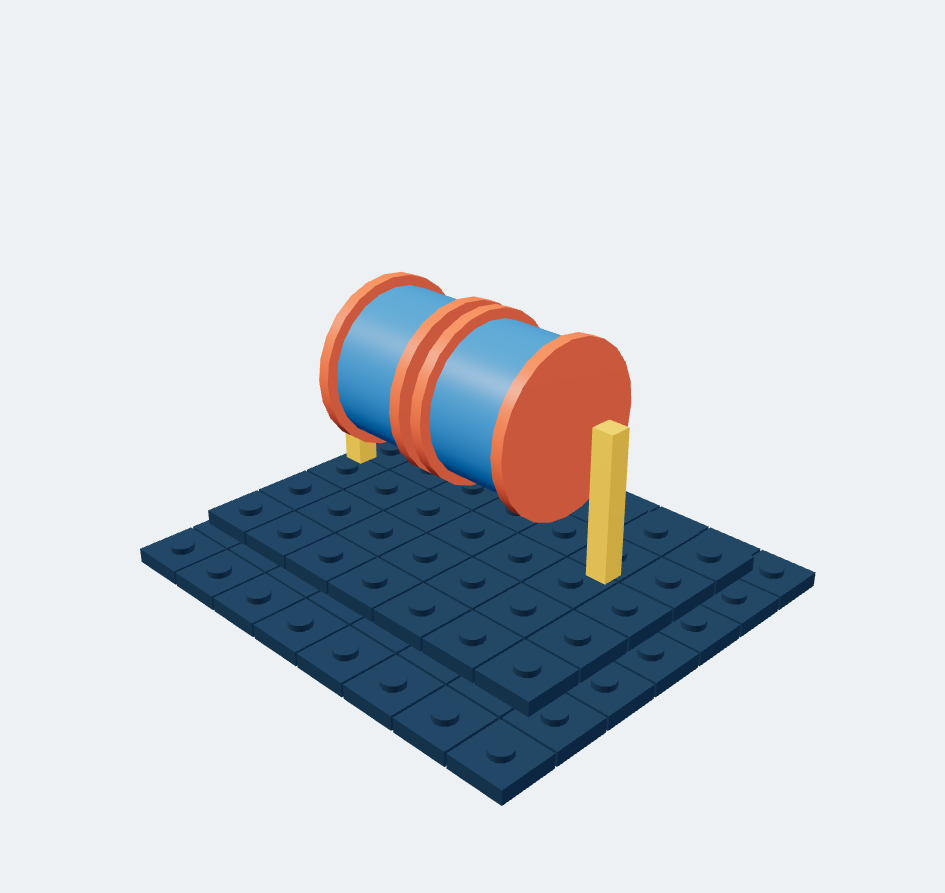
\includegraphics[width=.24\textwidth]{figures/hierarchy-expanded/exp-d1-drum-2-iso.png}
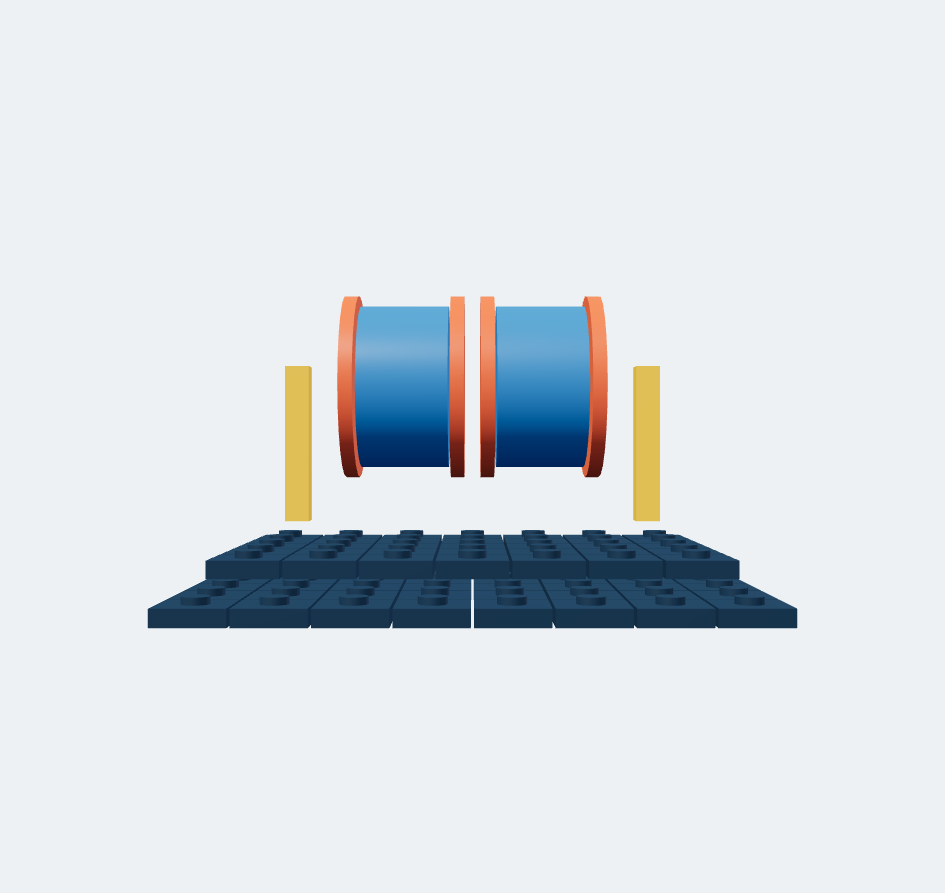
\includegraphics[width=.24\textwidth]{figures/hierarchy-expanded/exp-d1-drum-2-front.png}
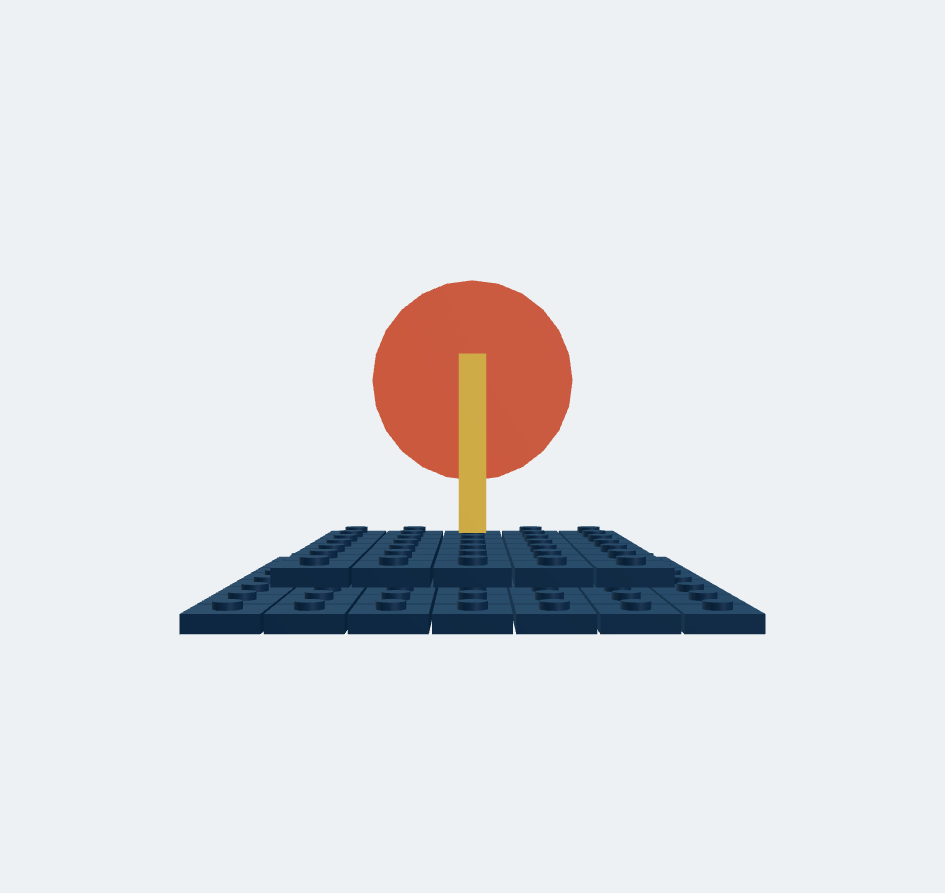
\includegraphics[width=.24\textwidth]{figures/hierarchy-expanded/exp-d1-drum-2-side.png}
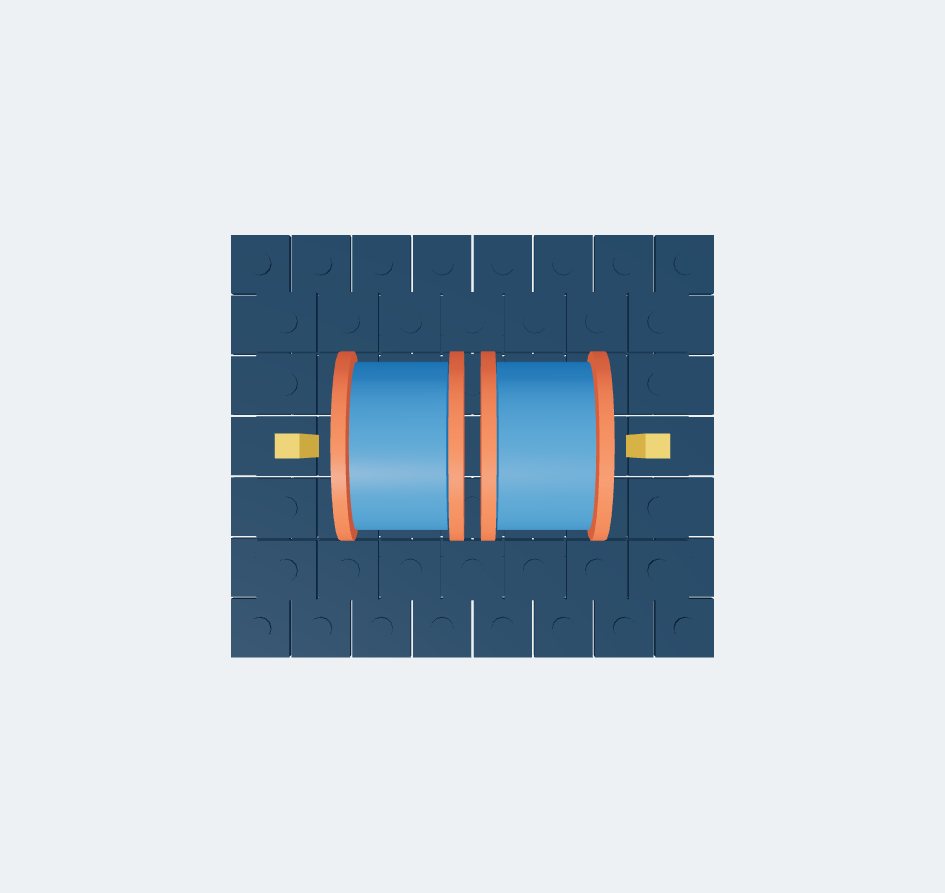
\includegraphics[width=.24\textwidth]{figures/hierarchy-expanded/exp-d1-drum-2-top.png}
\end{center}
\noindent All 48 families share this source. Full inputs and answers appear in the companion question bank.
\begin{center}\tiny\begin{tabular}{rllll}\toprule No. & Family & Layer & Output & Evidence\\\midrule
1 & identify & atomic & single-choice & model-state \\
2 & count & atomic & single-choice & model-state \\
3 & color & atomic & single-choice & model-state \\
4 & position & atomic & single-choice & model-state \\
5 & joint-type & atomic & single-choice & model-state \\
6 & parent & atomic & single-choice & model-state \\
7 & anchor & atomic & single-choice & model-state \\
8 & degree & atomic & single-choice & model-state \\
9 & recolor & atomic & single-choice & model-state \\
10 & add & atomic & single-choice & model-state \\
11 & remove & atomic & single-choice & model-state \\
12 & replace & atomic & single-choice & model-state \\
13 & translate & atomic & single-choice & model-state \\
14 & rotate & atomic & single-choice & model-state \\
15 & next-module & atomic & single-choice & model-state \\
16 & inventory & atomic & single-choice & model-state \\
17 & boundary & atomic & single-choice & model-state \\
18 & no-op & atomic & single-choice & model-state \\
19 & prefix & metacognitive & single-choice & support-graph \\
20 & access & metacognitive & multiple-choice & Rapier \\
21 & counterfactual & metacognitive & single-choice & support-graph \\
22 & dynamic & metacognitive & single-choice & Rapier \\
23 & kinematic & metacognitive & multiple-choice & model-state \\
24 & diagnosis & metacognitive & multiple-choice & model-state \\
25 & information-gain & metacognitive & multiple-choice & finite-world \\
26 & abstention & metacognitive & single-choice & finite-world \\
27 & posterior & metacognitive & single-choice & finite-world \\
28 & pareto & metacognitive & multiple-choice & model-state \\
29 & assembly & procedural & actions & state-machine \\
30 & disassembly & procedural & actions & state-machine \\
31 & service-repair & procedural & actions & state-machine \\
32 & compound-edit & procedural & actions & state-machine \\
33 & multi-fault & integrative & actions & state-machine \\
34 & scheduling & integrative & schedule & resource-schedule \\
35 & policy & integrative & policy & finite-world \\
36 & local-frame & atomic & single-choice & model-state \\
37 & projection & atomic & single-choice & model-state \\
38 & relative-order & atomic & single-choice & model-state \\
39 & joint-axis & atomic & single-choice & model-state \\
40 & clearance-margin & metacognitive & single-choice & model-state \\
41 & load-moment & metacognitive & single-choice & model-state \\
42 & weighted-posterior & metacognitive & single-choice & finite-world \\
43 & expected-loss & metacognitive & single-choice & finite-world \\
44 & trace-threshold & metacognitive & single-choice & Rapier \\
45 & guarded-repair & procedural & actions & state-machine \\
46 & rollback & procedural & actions & state-machine \\
47 & resource-repair & integrative & actions & state-machine \\
48 & budget-policy & integrative & policy & finite-world \\
\bottomrule\end{tabular}\end{center}
\clearpage
\subsection{10. Gantry Inspection Stage (D1)}
110 visible parts; 5 modules; 4 joints. Representative-point motion 0.0001; rotation 0.0000 rad.
\begin{center}
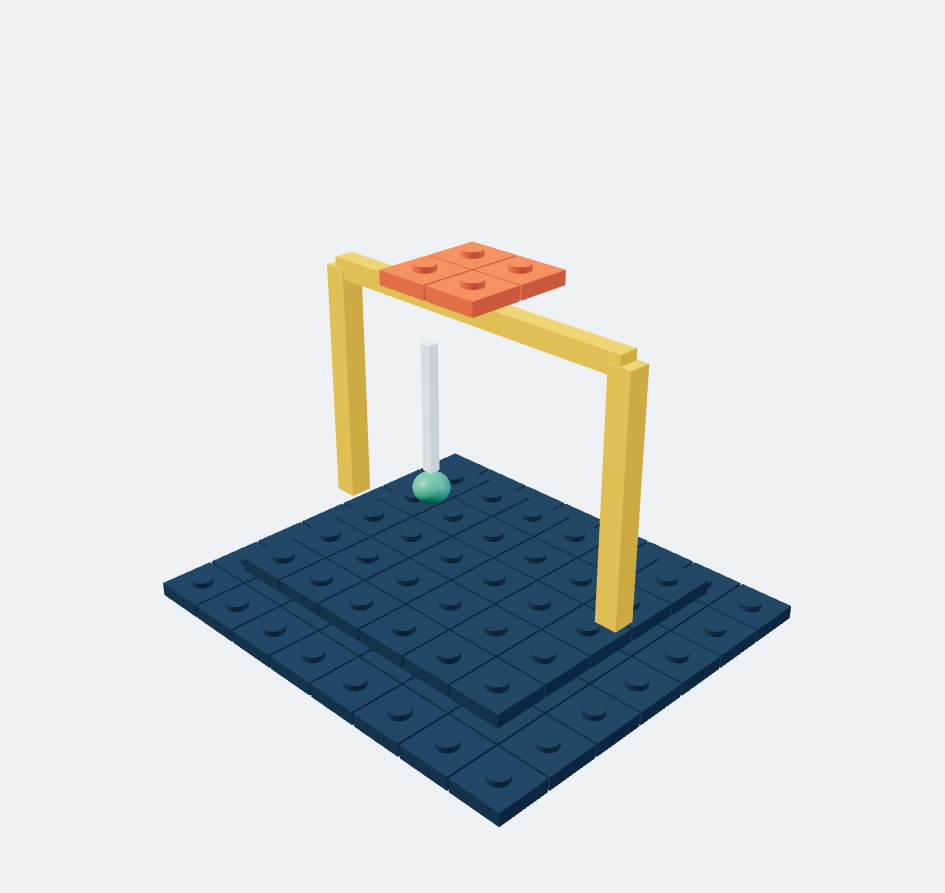
\includegraphics[width=.24\textwidth]{figures/hierarchy-expanded/exp-d1-gantry-1-iso.png}
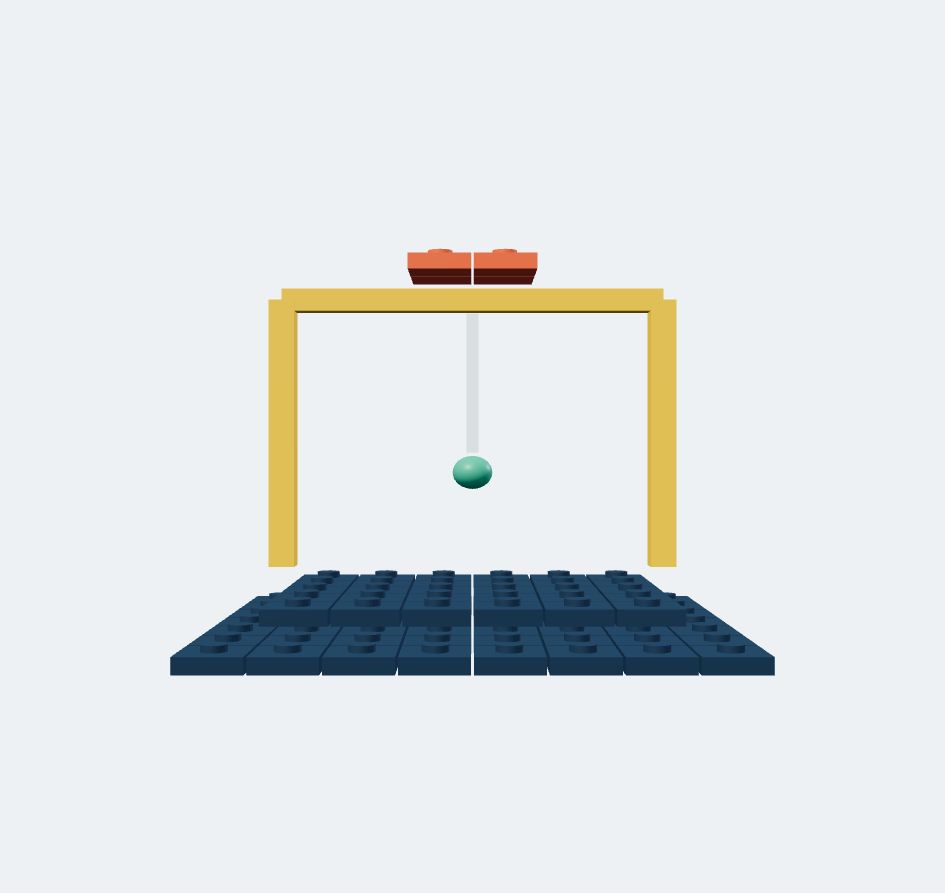
\includegraphics[width=.24\textwidth]{figures/hierarchy-expanded/exp-d1-gantry-1-front.png}
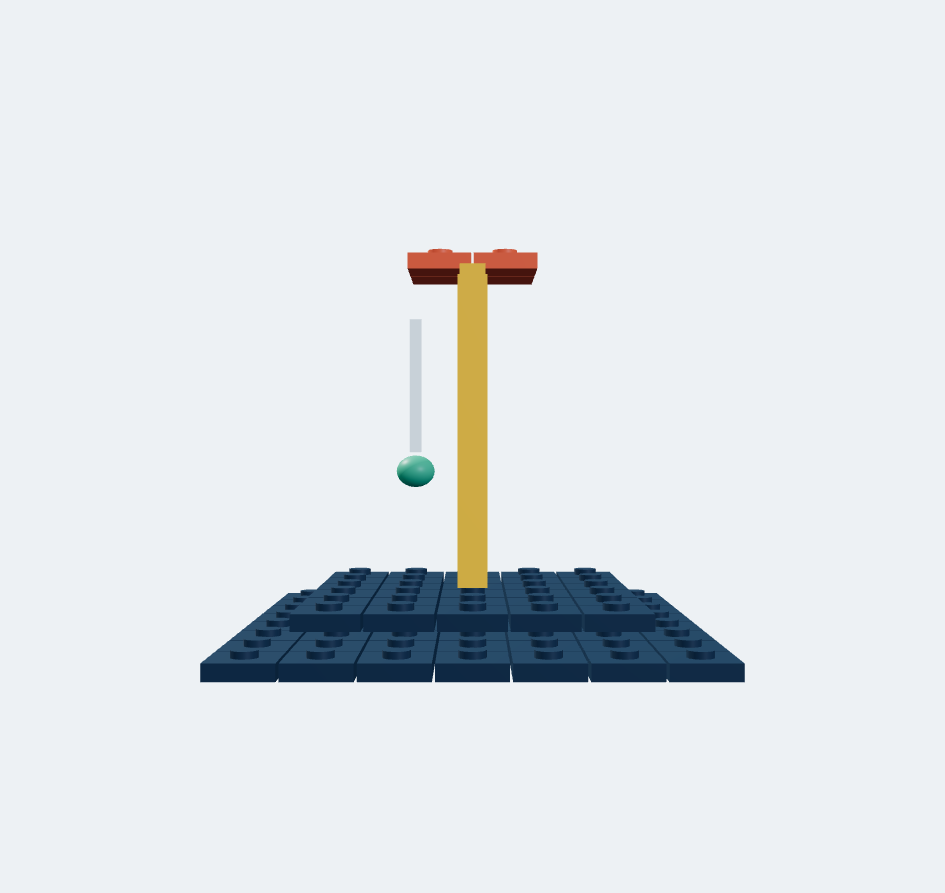
\includegraphics[width=.24\textwidth]{figures/hierarchy-expanded/exp-d1-gantry-1-side.png}
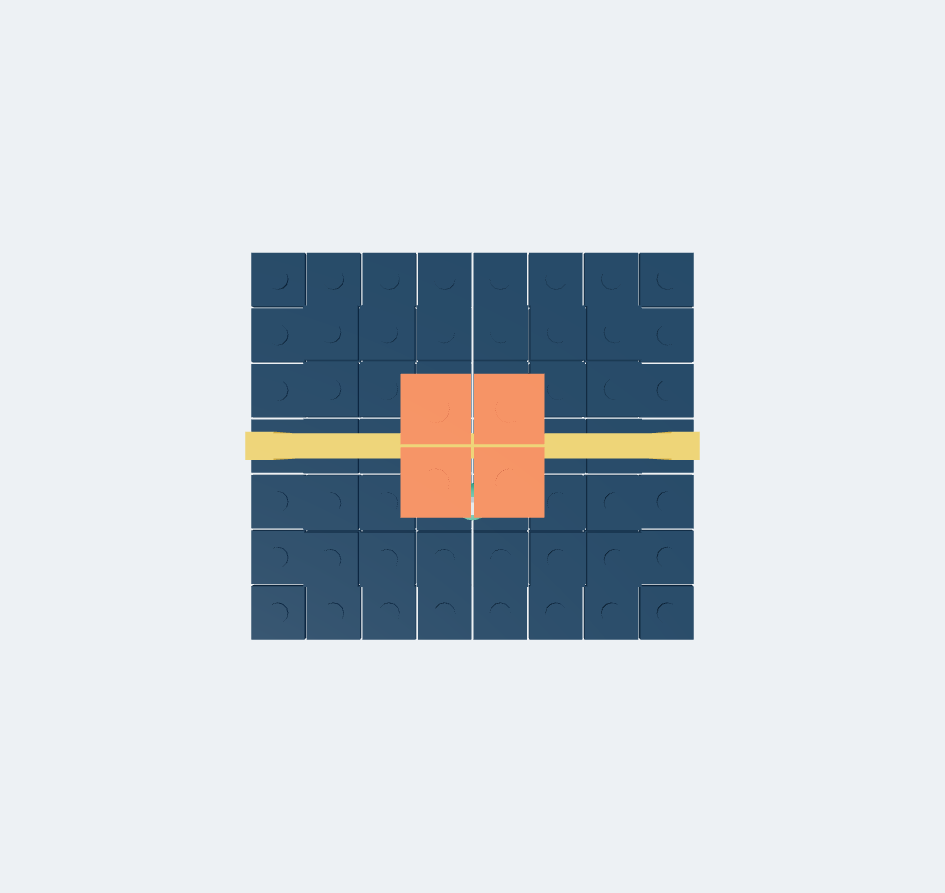
\includegraphics[width=.24\textwidth]{figures/hierarchy-expanded/exp-d1-gantry-1-top.png}
\end{center}
\noindent All 48 families share this source. Full inputs and answers appear in the companion question bank.
\begin{center}\tiny\begin{tabular}{rllll}\toprule No. & Family & Layer & Output & Evidence\\\midrule
1 & identify & atomic & single-choice & model-state \\
2 & count & atomic & single-choice & model-state \\
3 & color & atomic & single-choice & model-state \\
4 & position & atomic & single-choice & model-state \\
5 & joint-type & atomic & single-choice & model-state \\
6 & parent & atomic & single-choice & model-state \\
7 & anchor & atomic & single-choice & model-state \\
8 & degree & atomic & single-choice & model-state \\
9 & recolor & atomic & single-choice & model-state \\
10 & add & atomic & single-choice & model-state \\
11 & remove & atomic & single-choice & model-state \\
12 & replace & atomic & single-choice & model-state \\
13 & translate & atomic & single-choice & model-state \\
14 & rotate & atomic & single-choice & model-state \\
15 & next-module & atomic & single-choice & model-state \\
16 & inventory & atomic & single-choice & model-state \\
17 & boundary & atomic & single-choice & model-state \\
18 & no-op & atomic & single-choice & model-state \\
19 & prefix & metacognitive & single-choice & support-graph \\
20 & access & metacognitive & multiple-choice & Rapier \\
21 & counterfactual & metacognitive & single-choice & support-graph \\
22 & dynamic & metacognitive & single-choice & Rapier \\
23 & kinematic & metacognitive & multiple-choice & model-state \\
24 & diagnosis & metacognitive & multiple-choice & model-state \\
25 & information-gain & metacognitive & multiple-choice & finite-world \\
26 & abstention & metacognitive & single-choice & finite-world \\
27 & posterior & metacognitive & single-choice & finite-world \\
28 & pareto & metacognitive & multiple-choice & model-state \\
29 & assembly & procedural & actions & state-machine \\
30 & disassembly & procedural & actions & state-machine \\
31 & service-repair & procedural & actions & state-machine \\
32 & compound-edit & procedural & actions & state-machine \\
33 & multi-fault & integrative & actions & state-machine \\
34 & scheduling & integrative & schedule & resource-schedule \\
35 & policy & integrative & policy & finite-world \\
36 & local-frame & atomic & single-choice & model-state \\
37 & projection & atomic & single-choice & model-state \\
38 & relative-order & atomic & single-choice & model-state \\
39 & joint-axis & atomic & single-choice & model-state \\
40 & clearance-margin & metacognitive & single-choice & model-state \\
41 & load-moment & metacognitive & single-choice & model-state \\
42 & weighted-posterior & metacognitive & single-choice & finite-world \\
43 & expected-loss & metacognitive & single-choice & finite-world \\
44 & trace-threshold & metacognitive & single-choice & Rapier \\
45 & guarded-repair & procedural & actions & state-machine \\
46 & rollback & procedural & actions & state-machine \\
47 & resource-repair & integrative & actions & state-machine \\
48 & budget-policy & integrative & policy & finite-world \\
\bottomrule\end{tabular}\end{center}
\clearpage
\subsection{11. Twin-trolley Service Frame (D1)}
123 visible parts; 7 modules; 6 joints. Representative-point motion 0.0001; rotation 0.0000 rad.
\begin{center}
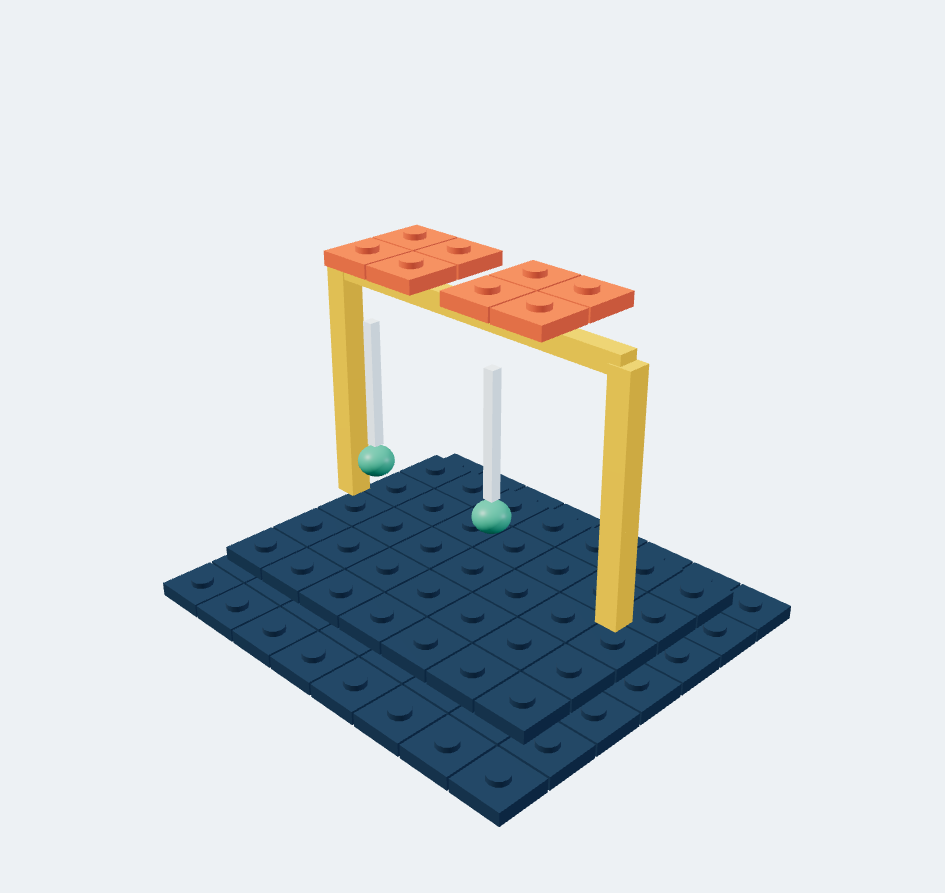
\includegraphics[width=.24\textwidth]{figures/hierarchy-expanded/exp-d1-gantry-2-iso.png}
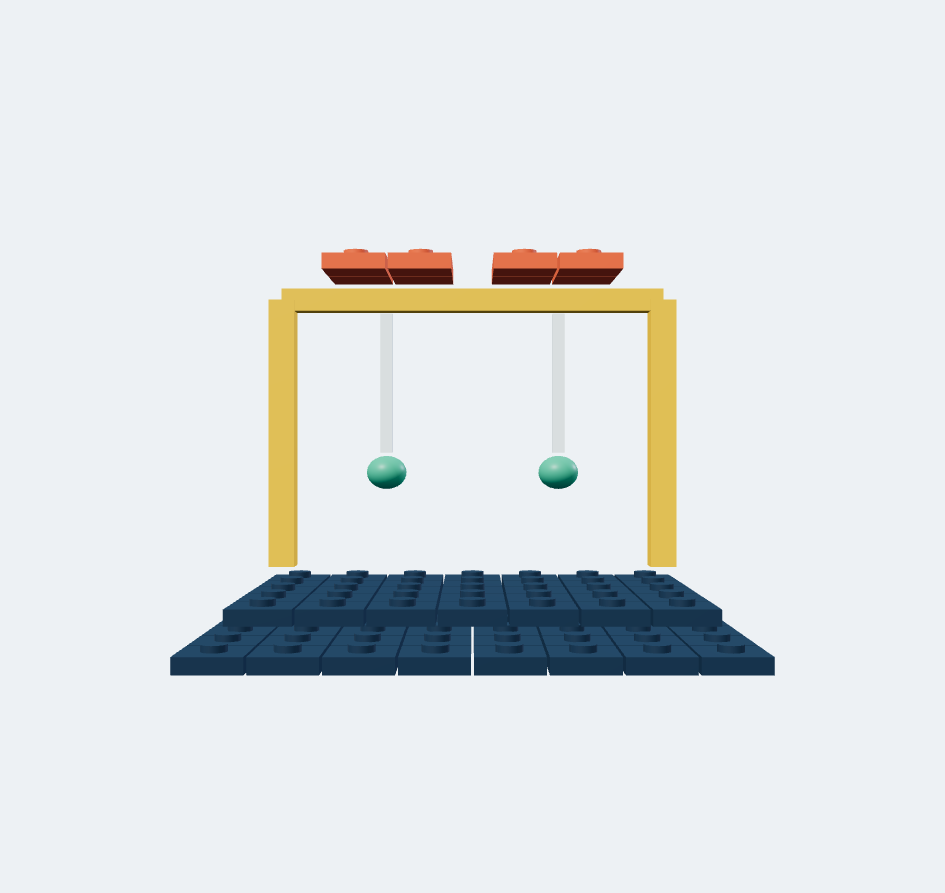
\includegraphics[width=.24\textwidth]{figures/hierarchy-expanded/exp-d1-gantry-2-front.png}
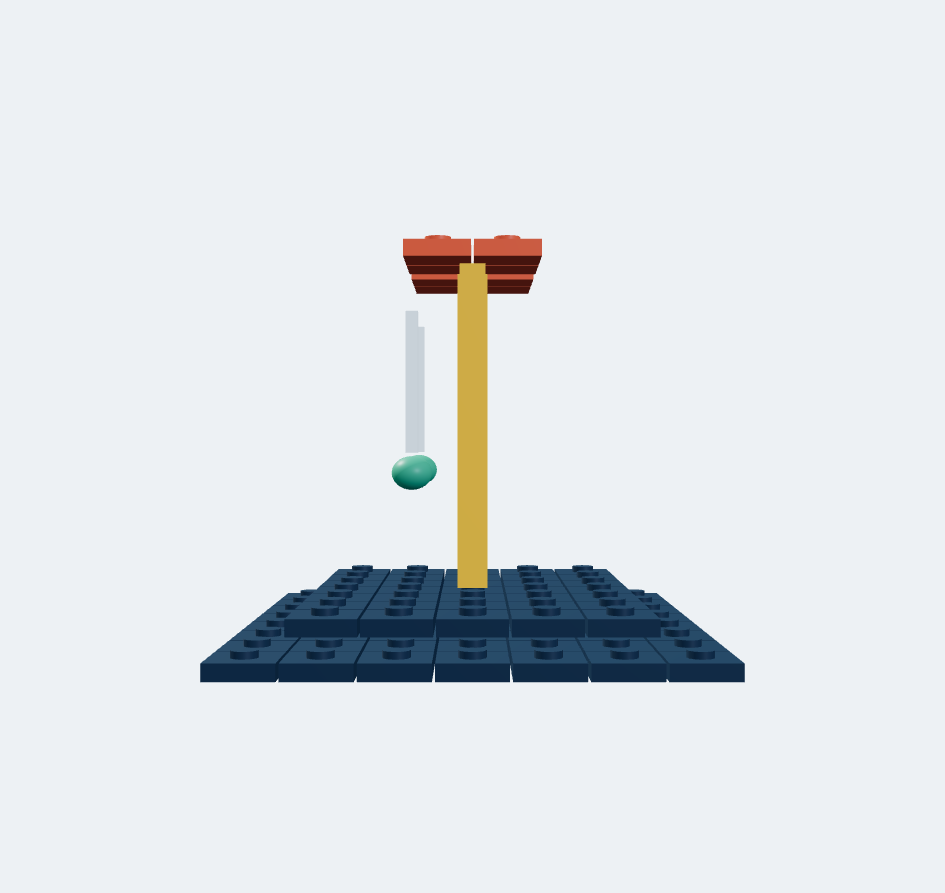
\includegraphics[width=.24\textwidth]{figures/hierarchy-expanded/exp-d1-gantry-2-side.png}
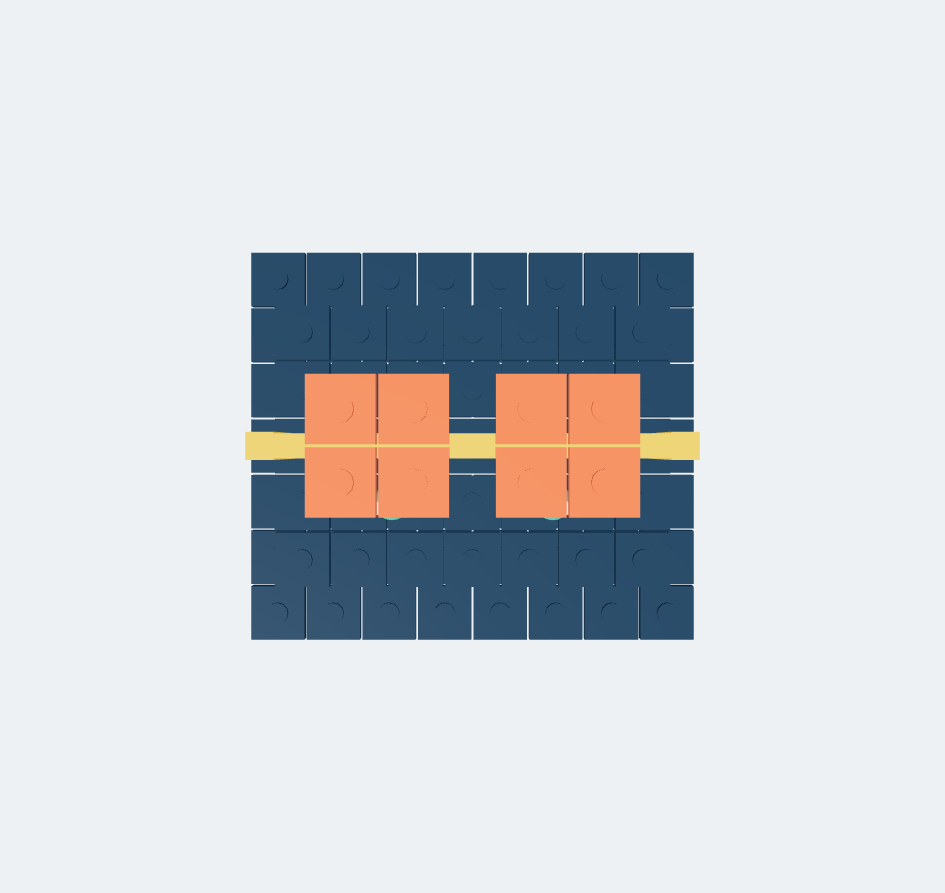
\includegraphics[width=.24\textwidth]{figures/hierarchy-expanded/exp-d1-gantry-2-top.png}
\end{center}
\noindent All 48 families share this source. Full inputs and answers appear in the companion question bank.
\begin{center}\tiny\begin{tabular}{rllll}\toprule No. & Family & Layer & Output & Evidence\\\midrule
1 & identify & atomic & single-choice & model-state \\
2 & count & atomic & single-choice & model-state \\
3 & color & atomic & single-choice & model-state \\
4 & position & atomic & single-choice & model-state \\
5 & joint-type & atomic & single-choice & model-state \\
6 & parent & atomic & single-choice & model-state \\
7 & anchor & atomic & single-choice & model-state \\
8 & degree & atomic & single-choice & model-state \\
9 & recolor & atomic & single-choice & model-state \\
10 & add & atomic & single-choice & model-state \\
11 & remove & atomic & single-choice & model-state \\
12 & replace & atomic & single-choice & model-state \\
13 & translate & atomic & single-choice & model-state \\
14 & rotate & atomic & single-choice & model-state \\
15 & next-module & atomic & single-choice & model-state \\
16 & inventory & atomic & single-choice & model-state \\
17 & boundary & atomic & single-choice & model-state \\
18 & no-op & atomic & single-choice & model-state \\
19 & prefix & metacognitive & single-choice & support-graph \\
20 & access & metacognitive & multiple-choice & Rapier \\
21 & counterfactual & metacognitive & single-choice & support-graph \\
22 & dynamic & metacognitive & single-choice & Rapier \\
23 & kinematic & metacognitive & multiple-choice & model-state \\
24 & diagnosis & metacognitive & multiple-choice & model-state \\
25 & information-gain & metacognitive & multiple-choice & finite-world \\
26 & abstention & metacognitive & single-choice & finite-world \\
27 & posterior & metacognitive & single-choice & finite-world \\
28 & pareto & metacognitive & multiple-choice & model-state \\
29 & assembly & procedural & actions & state-machine \\
30 & disassembly & procedural & actions & state-machine \\
31 & service-repair & procedural & actions & state-machine \\
32 & compound-edit & procedural & actions & state-machine \\
33 & multi-fault & integrative & actions & state-machine \\
34 & scheduling & integrative & schedule & resource-schedule \\
35 & policy & integrative & policy & finite-world \\
36 & local-frame & atomic & single-choice & model-state \\
37 & projection & atomic & single-choice & model-state \\
38 & relative-order & atomic & single-choice & model-state \\
39 & joint-axis & atomic & single-choice & model-state \\
40 & clearance-margin & metacognitive & single-choice & model-state \\
41 & load-moment & metacognitive & single-choice & model-state \\
42 & weighted-posterior & metacognitive & single-choice & finite-world \\
43 & expected-loss & metacognitive & single-choice & finite-world \\
44 & trace-threshold & metacognitive & single-choice & Rapier \\
45 & guarded-repair & procedural & actions & state-machine \\
46 & rollback & procedural & actions & state-machine \\
47 & resource-repair & integrative & actions & state-machine \\
48 & budget-policy & integrative & policy & finite-world \\
\bottomrule\end{tabular}\end{center}
\clearpage
\subsection{12. Rotary Sector Gate (D1)}
103 visible parts; 3 modules; 2 joints. Representative-point motion 0.0000; rotation 0.0000 rad.
\begin{center}
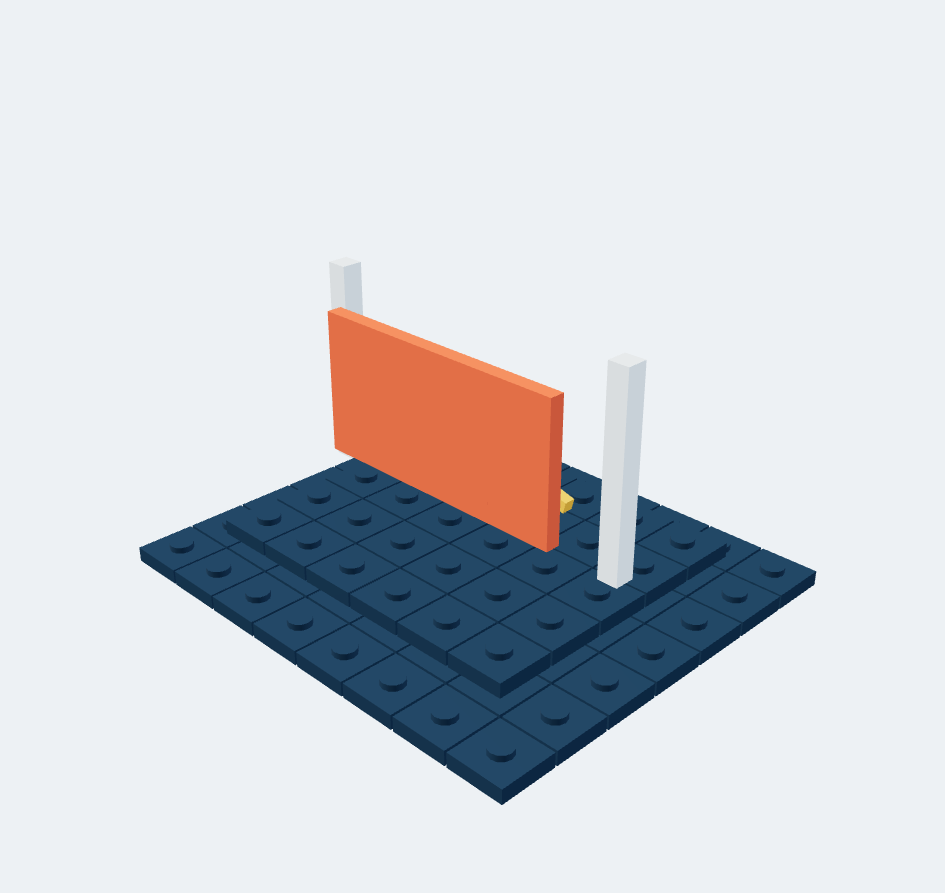
\includegraphics[width=.24\textwidth]{figures/hierarchy-expanded/exp-d1-gate-1-iso.png}

\includegraphics[width=.24\textwidth]{figures/hierarchy-expanded/exp-d1-gate-1-front.png}
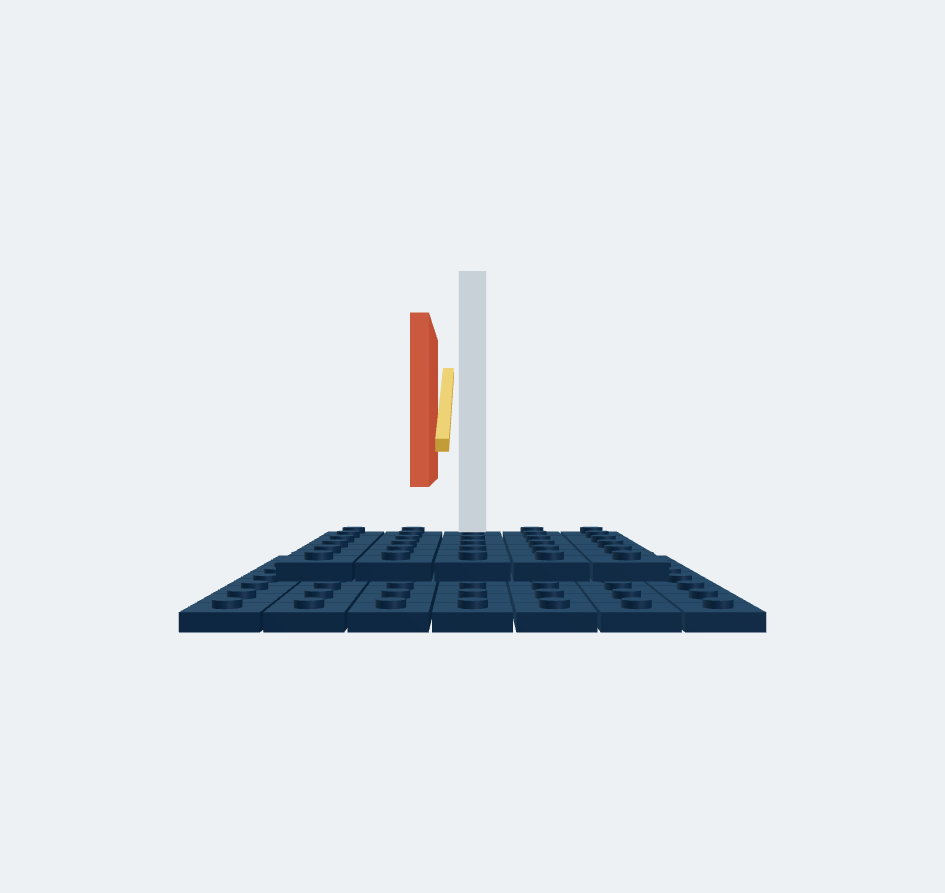
\includegraphics[width=.24\textwidth]{figures/hierarchy-expanded/exp-d1-gate-1-side.png}
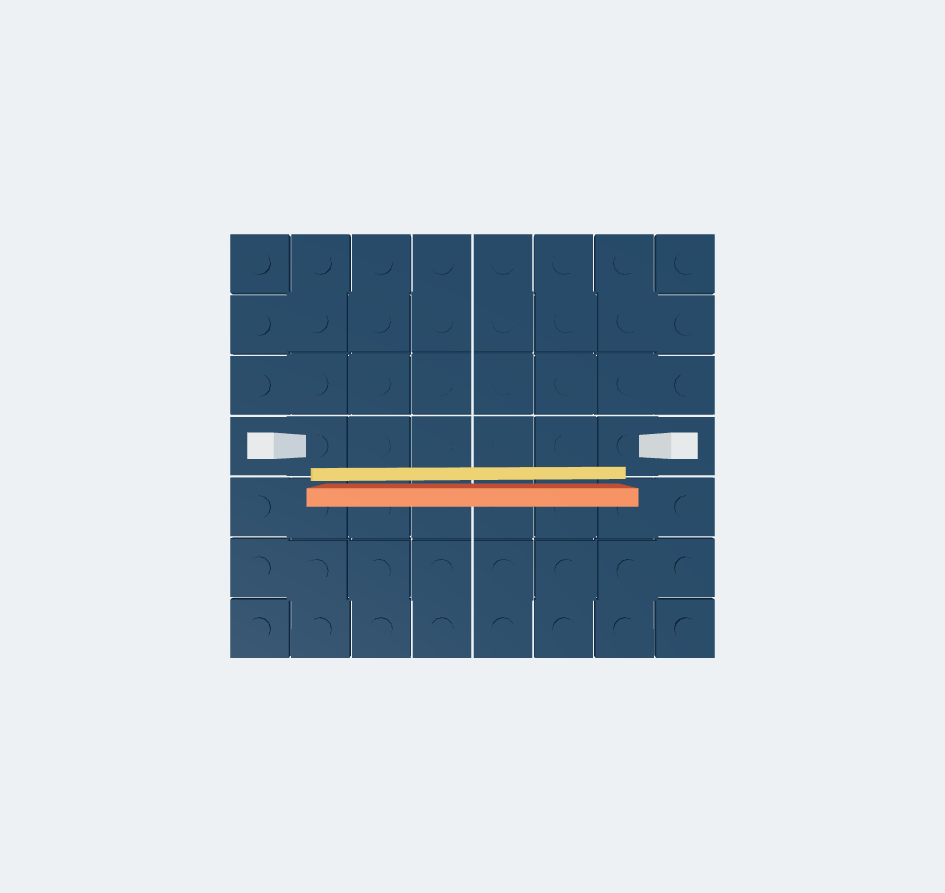
\includegraphics[width=.24\textwidth]{figures/hierarchy-expanded/exp-d1-gate-1-top.png}
\end{center}
\noindent All 48 families share this source. Full inputs and answers appear in the companion question bank.
\begin{center}\tiny\begin{tabular}{rllll}\toprule No. & Family & Layer & Output & Evidence\\\midrule
1 & identify & atomic & single-choice & model-state \\
2 & count & atomic & single-choice & model-state \\
3 & color & atomic & single-choice & model-state \\
4 & position & atomic & single-choice & model-state \\
5 & joint-type & atomic & single-choice & model-state \\
6 & parent & atomic & single-choice & model-state \\
7 & anchor & atomic & single-choice & model-state \\
8 & degree & atomic & single-choice & model-state \\
9 & recolor & atomic & single-choice & model-state \\
10 & add & atomic & single-choice & model-state \\
11 & remove & atomic & single-choice & model-state \\
12 & replace & atomic & single-choice & model-state \\
13 & translate & atomic & single-choice & model-state \\
14 & rotate & atomic & single-choice & model-state \\
15 & next-module & atomic & single-choice & model-state \\
16 & inventory & atomic & single-choice & model-state \\
17 & boundary & atomic & single-choice & model-state \\
18 & no-op & atomic & single-choice & model-state \\
19 & prefix & metacognitive & single-choice & support-graph \\
20 & access & metacognitive & multiple-choice & Rapier \\
21 & counterfactual & metacognitive & single-choice & support-graph \\
22 & dynamic & metacognitive & single-choice & Rapier \\
23 & kinematic & metacognitive & multiple-choice & model-state \\
24 & diagnosis & metacognitive & multiple-choice & model-state \\
25 & information-gain & metacognitive & multiple-choice & finite-world \\
26 & abstention & metacognitive & single-choice & finite-world \\
27 & posterior & metacognitive & single-choice & finite-world \\
28 & pareto & metacognitive & multiple-choice & model-state \\
29 & assembly & procedural & actions & state-machine \\
30 & disassembly & procedural & actions & state-machine \\
31 & service-repair & procedural & actions & state-machine \\
32 & compound-edit & procedural & actions & state-machine \\
33 & multi-fault & integrative & actions & state-machine \\
34 & scheduling & integrative & schedule & resource-schedule \\
35 & policy & integrative & policy & finite-world \\
36 & local-frame & atomic & single-choice & model-state \\
37 & projection & atomic & single-choice & model-state \\
38 & relative-order & atomic & single-choice & model-state \\
39 & joint-axis & atomic & single-choice & model-state \\
40 & clearance-margin & metacognitive & single-choice & model-state \\
41 & load-moment & metacognitive & single-choice & model-state \\
42 & weighted-posterior & metacognitive & single-choice & finite-world \\
43 & expected-loss & metacognitive & single-choice & finite-world \\
44 & trace-threshold & metacognitive & single-choice & Rapier \\
45 & guarded-repair & procedural & actions & state-machine \\
46 & rollback & procedural & actions & state-machine \\
47 & resource-repair & integrative & actions & state-machine \\
48 & budget-policy & integrative & policy & finite-world \\
\bottomrule\end{tabular}\end{center}
\clearpage
\subsection{13. Twin-leaf Interlock Frame (D1)}
113 visible parts; 4 modules; 3 joints. Representative-point motion 0.0000; rotation 0.0000 rad.
\begin{center}
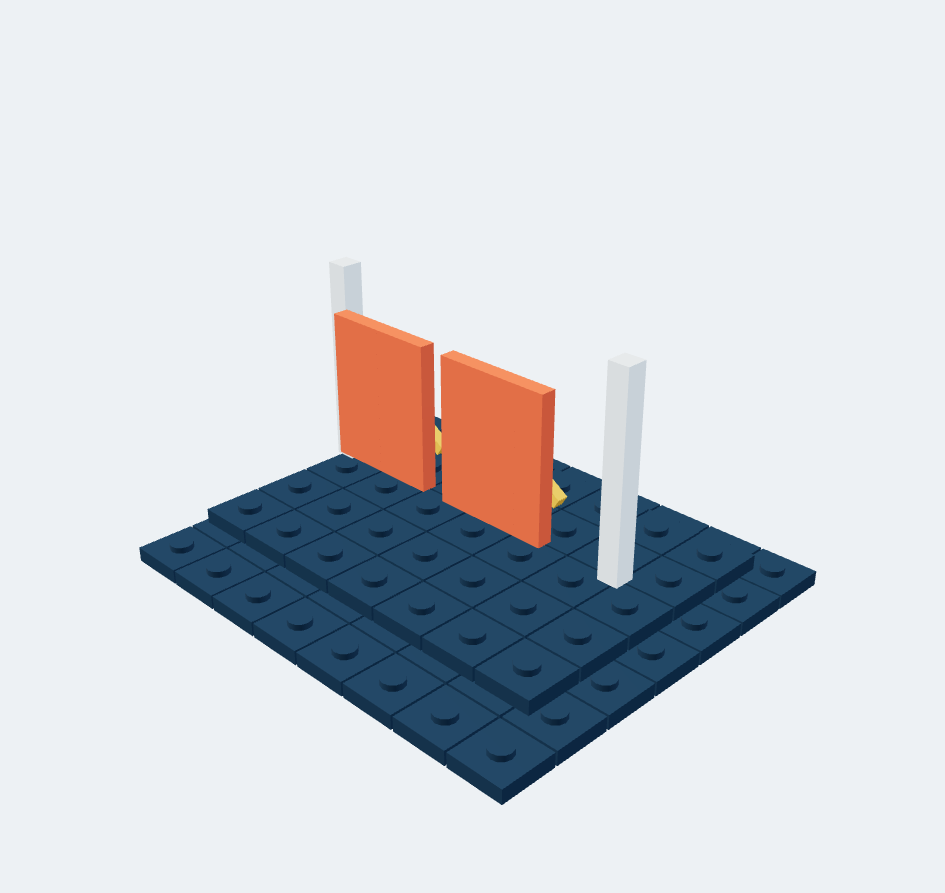
\includegraphics[width=.24\textwidth]{figures/hierarchy-expanded/exp-d1-gate-2-iso.png}

\includegraphics[width=.24\textwidth]{figures/hierarchy-expanded/exp-d1-gate-2-front.png}
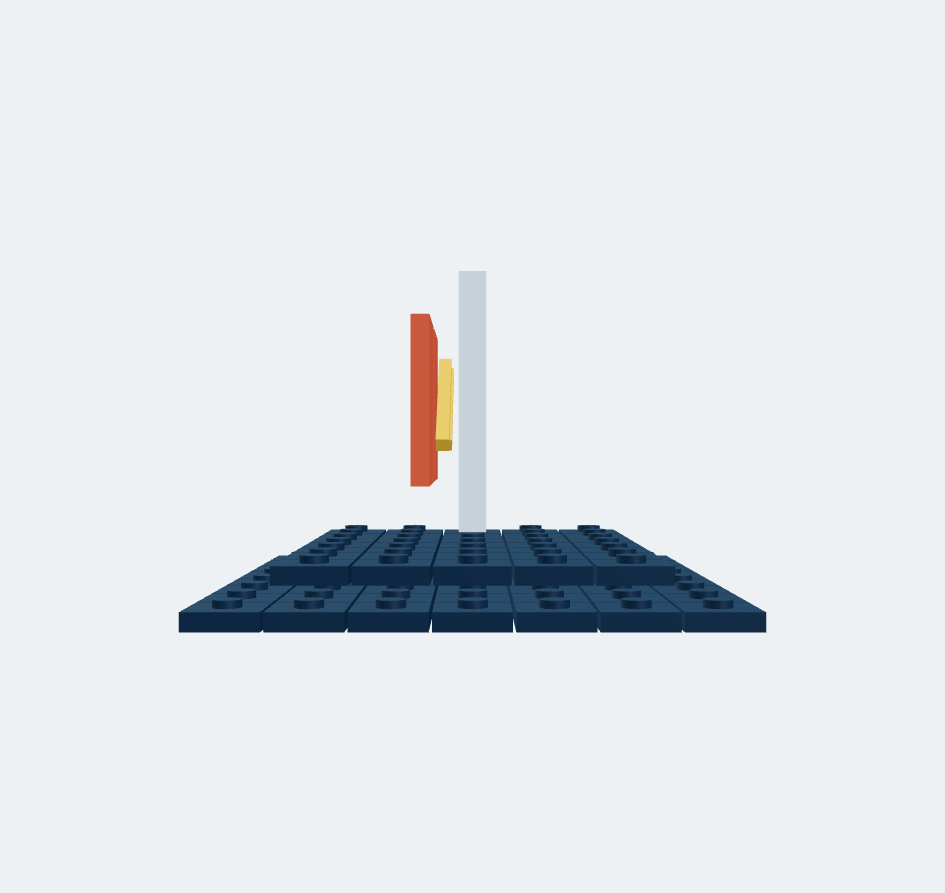
\includegraphics[width=.24\textwidth]{figures/hierarchy-expanded/exp-d1-gate-2-side.png}
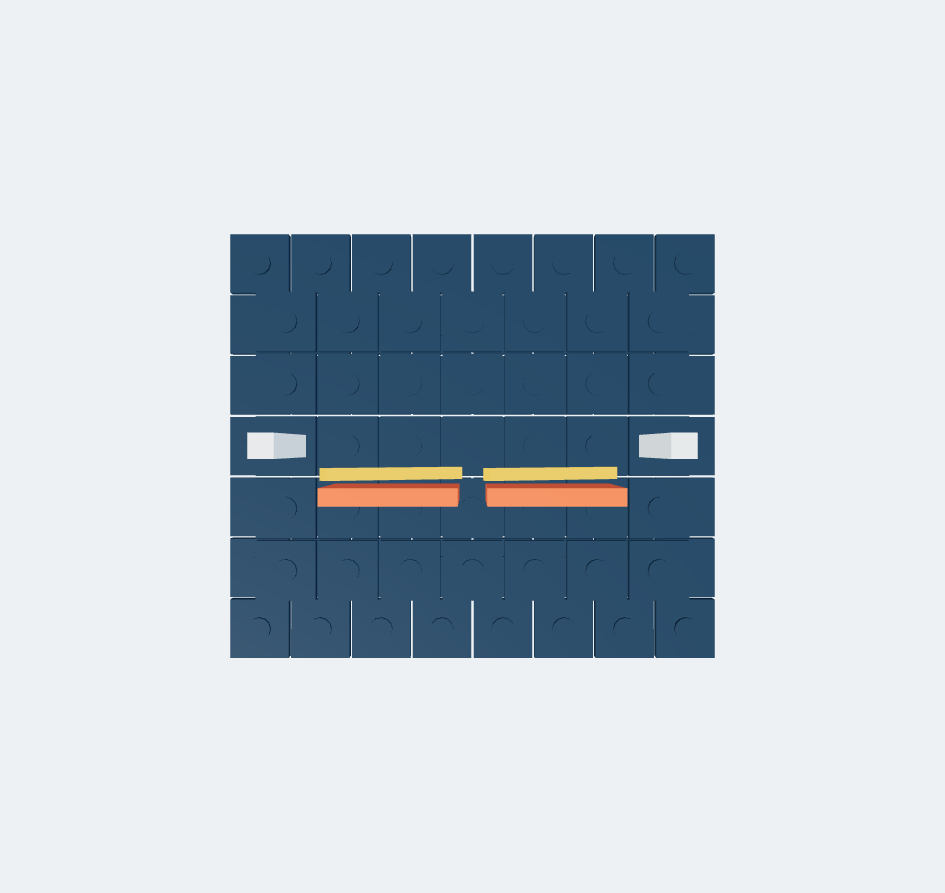
\includegraphics[width=.24\textwidth]{figures/hierarchy-expanded/exp-d1-gate-2-top.png}
\end{center}
\noindent All 48 families share this source. Full inputs and answers appear in the companion question bank.
\begin{center}\tiny\begin{tabular}{rllll}\toprule No. & Family & Layer & Output & Evidence\\\midrule
1 & identify & atomic & single-choice & model-state \\
2 & count & atomic & single-choice & model-state \\
3 & color & atomic & single-choice & model-state \\
4 & position & atomic & single-choice & model-state \\
5 & joint-type & atomic & single-choice & model-state \\
6 & parent & atomic & single-choice & model-state \\
7 & anchor & atomic & single-choice & model-state \\
8 & degree & atomic & single-choice & model-state \\
9 & recolor & atomic & single-choice & model-state \\
10 & add & atomic & single-choice & model-state \\
11 & remove & atomic & single-choice & model-state \\
12 & replace & atomic & single-choice & model-state \\
13 & translate & atomic & single-choice & model-state \\
14 & rotate & atomic & single-choice & model-state \\
15 & next-module & atomic & single-choice & model-state \\
16 & inventory & atomic & single-choice & model-state \\
17 & boundary & atomic & single-choice & model-state \\
18 & no-op & atomic & single-choice & model-state \\
19 & prefix & metacognitive & single-choice & support-graph \\
20 & access & metacognitive & multiple-choice & Rapier \\
21 & counterfactual & metacognitive & single-choice & support-graph \\
22 & dynamic & metacognitive & single-choice & Rapier \\
23 & kinematic & metacognitive & multiple-choice & model-state \\
24 & diagnosis & metacognitive & multiple-choice & model-state \\
25 & information-gain & metacognitive & multiple-choice & finite-world \\
26 & abstention & metacognitive & single-choice & finite-world \\
27 & posterior & metacognitive & single-choice & finite-world \\
28 & pareto & metacognitive & multiple-choice & model-state \\
29 & assembly & procedural & actions & state-machine \\
30 & disassembly & procedural & actions & state-machine \\
31 & service-repair & procedural & actions & state-machine \\
32 & compound-edit & procedural & actions & state-machine \\
33 & multi-fault & integrative & actions & state-machine \\
34 & scheduling & integrative & schedule & resource-schedule \\
35 & policy & integrative & policy & finite-world \\
36 & local-frame & atomic & single-choice & model-state \\
37 & projection & atomic & single-choice & model-state \\
38 & relative-order & atomic & single-choice & model-state \\
39 & joint-axis & atomic & single-choice & model-state \\
40 & clearance-margin & metacognitive & single-choice & model-state \\
41 & load-moment & metacognitive & single-choice & model-state \\
42 & weighted-posterior & metacognitive & single-choice & finite-world \\
43 & expected-loss & metacognitive & single-choice & finite-world \\
44 & trace-threshold & metacognitive & single-choice & Rapier \\
45 & guarded-repair & procedural & actions & state-machine \\
46 & rollback & procedural & actions & state-machine \\
47 & resource-repair & integrative & actions & state-machine \\
48 & budget-policy & integrative & policy & finite-world \\
\bottomrule\end{tabular}\end{center}
\clearpage
\subsection{14. Opposed Gripper (D1)}
93 visible parts; 5 modules; 4 joints. Representative-point motion 0.0001; rotation 0.0000 rad.
\begin{center}
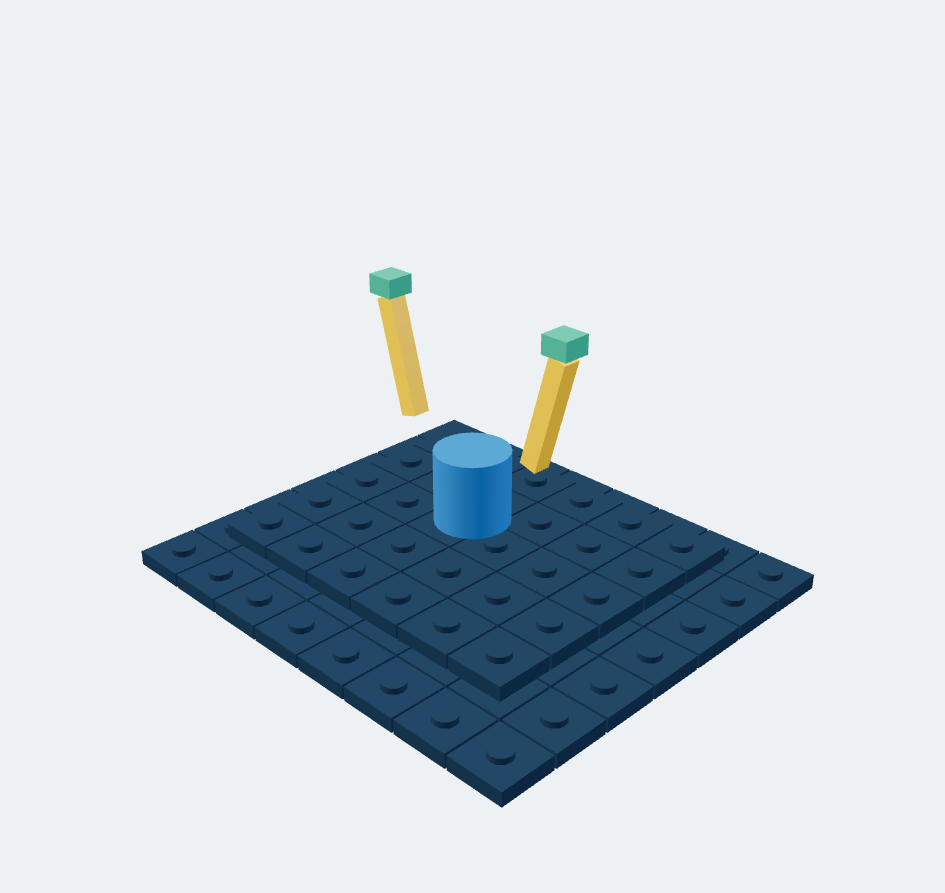
\includegraphics[width=.24\textwidth]{figures/hierarchy-expanded/exp-d1-gripper-1-iso.png}
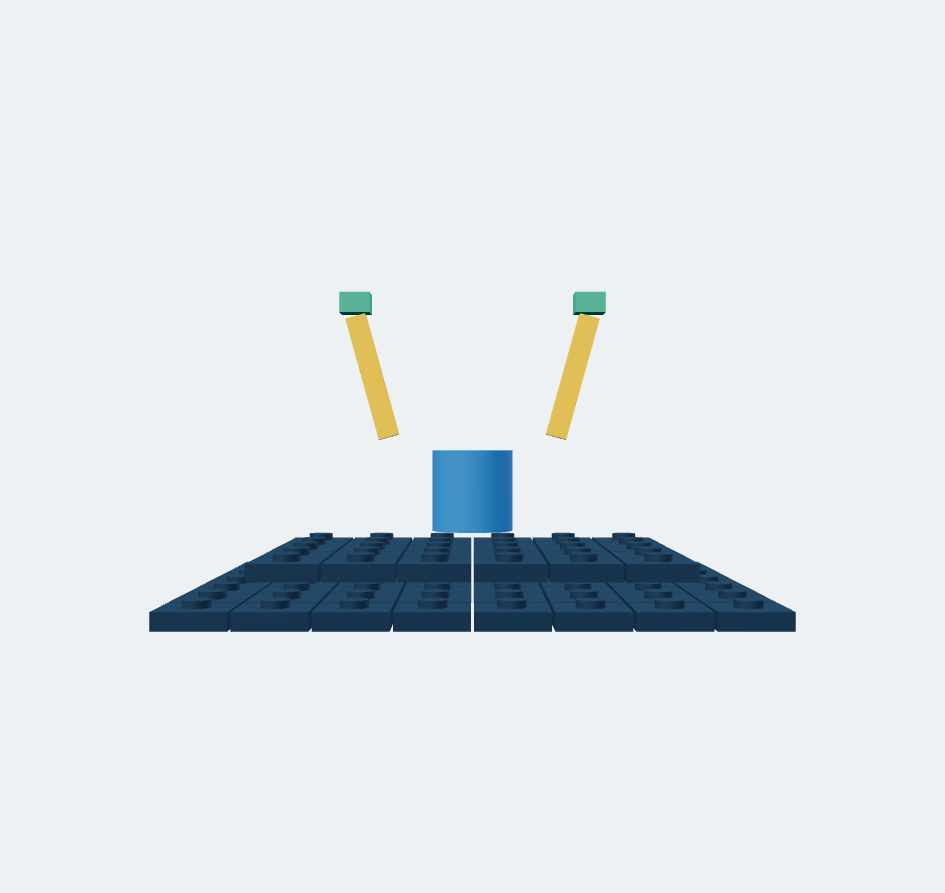
\includegraphics[width=.24\textwidth]{figures/hierarchy-expanded/exp-d1-gripper-1-front.png}
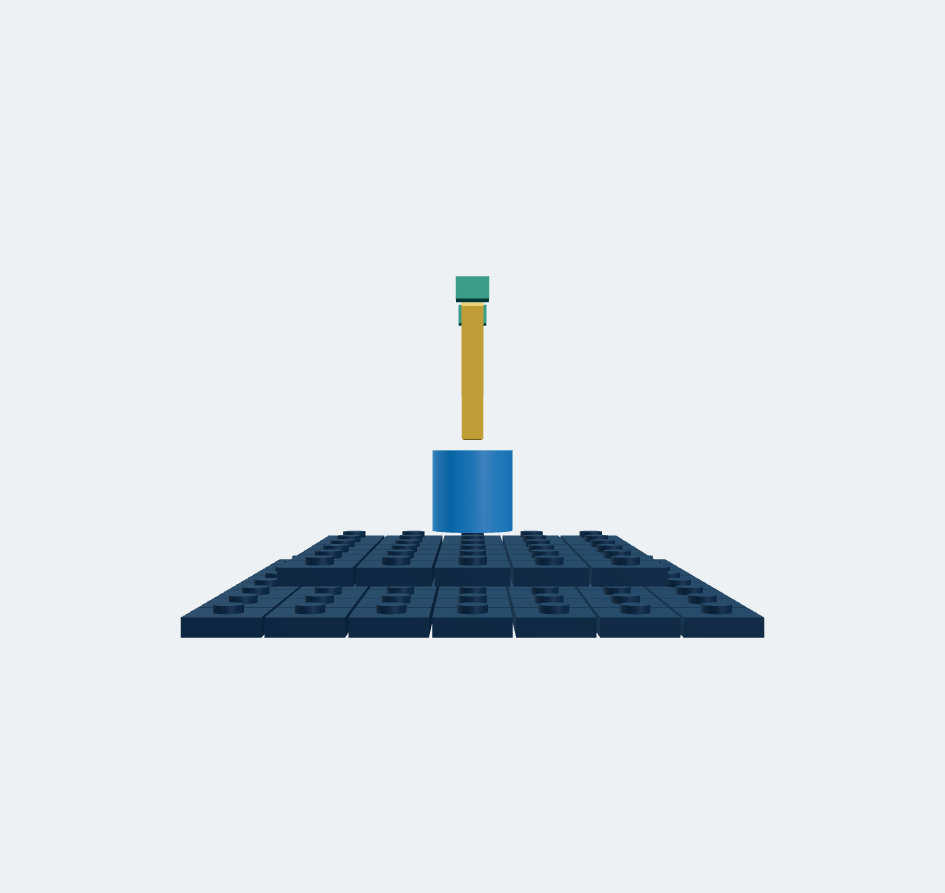
\includegraphics[width=.24\textwidth]{figures/hierarchy-expanded/exp-d1-gripper-1-side.png}
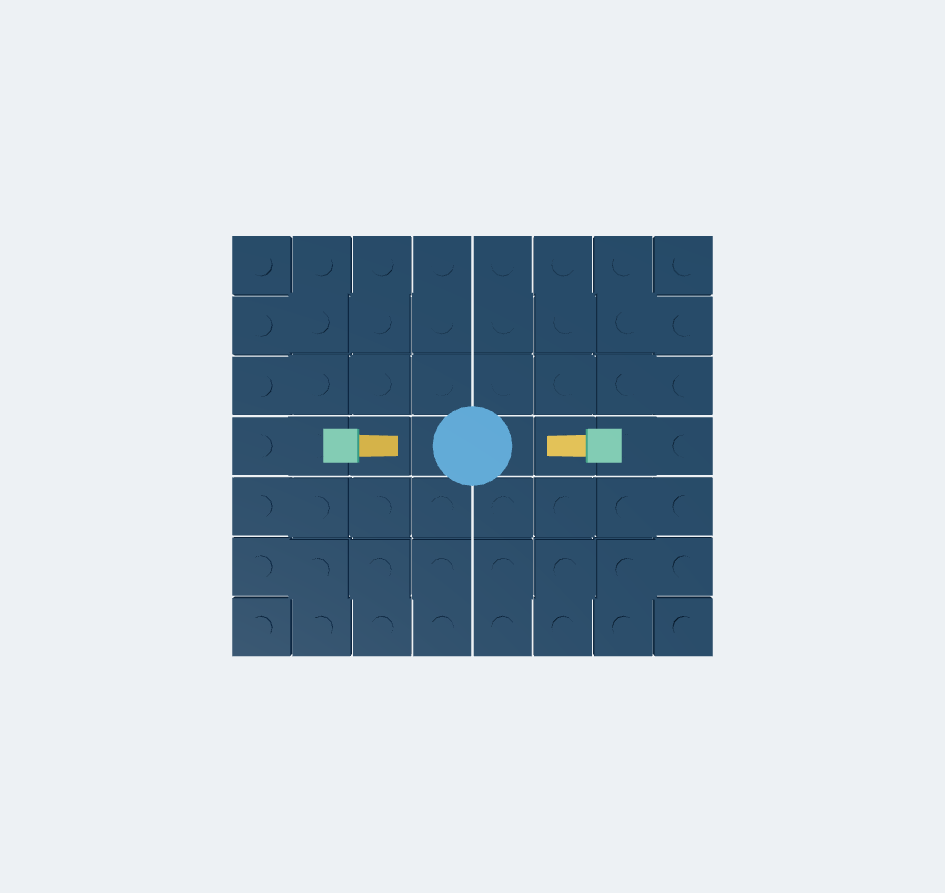
\includegraphics[width=.24\textwidth]{figures/hierarchy-expanded/exp-d1-gripper-1-top.png}
\end{center}
\noindent All 48 families share this source. Full inputs and answers appear in the companion question bank.
\begin{center}\tiny\begin{tabular}{rllll}\toprule No. & Family & Layer & Output & Evidence\\\midrule
1 & identify & atomic & single-choice & model-state \\
2 & count & atomic & single-choice & model-state \\
3 & color & atomic & single-choice & model-state \\
4 & position & atomic & single-choice & model-state \\
5 & joint-type & atomic & single-choice & model-state \\
6 & parent & atomic & single-choice & model-state \\
7 & anchor & atomic & single-choice & model-state \\
8 & degree & atomic & single-choice & model-state \\
9 & recolor & atomic & single-choice & model-state \\
10 & add & atomic & single-choice & model-state \\
11 & remove & atomic & single-choice & model-state \\
12 & replace & atomic & single-choice & model-state \\
13 & translate & atomic & single-choice & model-state \\
14 & rotate & atomic & single-choice & model-state \\
15 & next-module & atomic & single-choice & model-state \\
16 & inventory & atomic & single-choice & model-state \\
17 & boundary & atomic & single-choice & model-state \\
18 & no-op & atomic & single-choice & model-state \\
19 & prefix & metacognitive & single-choice & support-graph \\
20 & access & metacognitive & multiple-choice & Rapier \\
21 & counterfactual & metacognitive & single-choice & support-graph \\
22 & dynamic & metacognitive & single-choice & Rapier \\
23 & kinematic & metacognitive & multiple-choice & model-state \\
24 & diagnosis & metacognitive & multiple-choice & model-state \\
25 & information-gain & metacognitive & multiple-choice & finite-world \\
26 & abstention & metacognitive & single-choice & finite-world \\
27 & posterior & metacognitive & single-choice & finite-world \\
28 & pareto & metacognitive & multiple-choice & model-state \\
29 & assembly & procedural & actions & state-machine \\
30 & disassembly & procedural & actions & state-machine \\
31 & service-repair & procedural & actions & state-machine \\
32 & compound-edit & procedural & actions & state-machine \\
33 & multi-fault & integrative & actions & state-machine \\
34 & scheduling & integrative & schedule & resource-schedule \\
35 & policy & integrative & policy & finite-world \\
36 & local-frame & atomic & single-choice & model-state \\
37 & projection & atomic & single-choice & model-state \\
38 & relative-order & atomic & single-choice & model-state \\
39 & joint-axis & atomic & single-choice & model-state \\
40 & clearance-margin & metacognitive & single-choice & model-state \\
41 & load-moment & metacognitive & single-choice & model-state \\
42 & weighted-posterior & metacognitive & single-choice & finite-world \\
43 & expected-loss & metacognitive & single-choice & finite-world \\
44 & trace-threshold & metacognitive & single-choice & Rapier \\
45 & guarded-repair & procedural & actions & state-machine \\
46 & rollback & procedural & actions & state-machine \\
47 & resource-repair & integrative & actions & state-machine \\
48 & budget-policy & integrative & policy & finite-world \\
\bottomrule\end{tabular}\end{center}
\clearpage
\subsection{15. Three-finger Gripper (D1)}
101 visible parts; 6 modules; 5 joints. Representative-point motion 0.0001; rotation 0.0000 rad.
\begin{center}
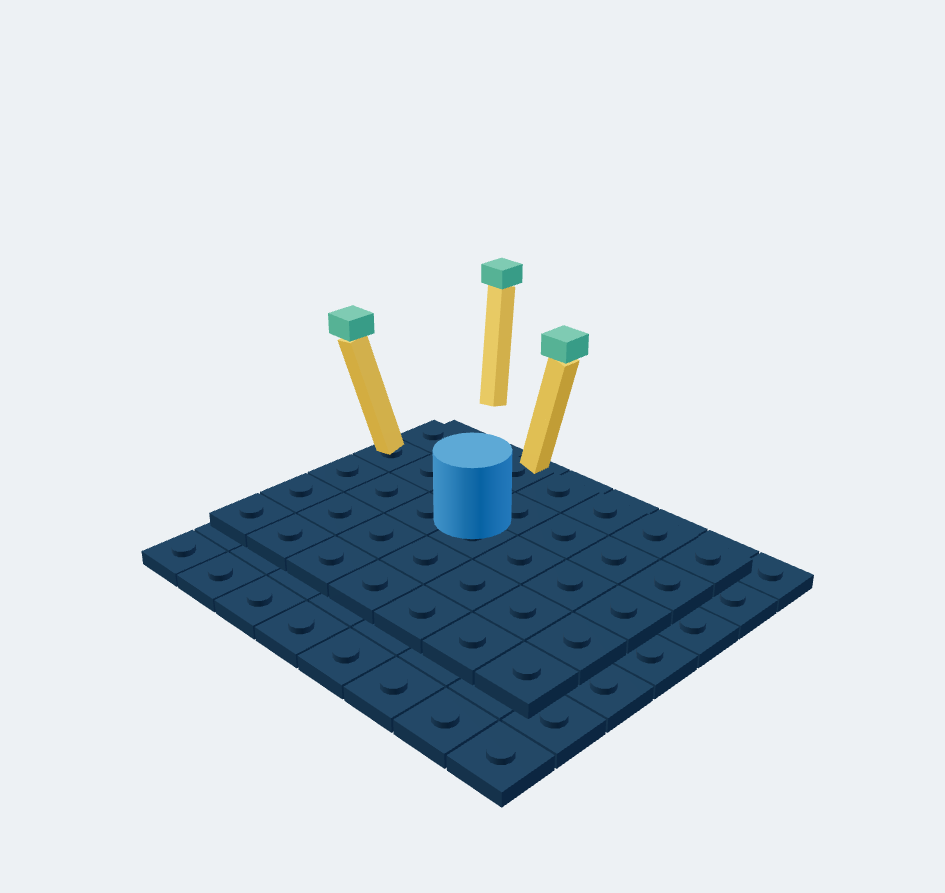
\includegraphics[width=.24\textwidth]{figures/hierarchy-expanded/exp-d1-gripper-2-iso.png}
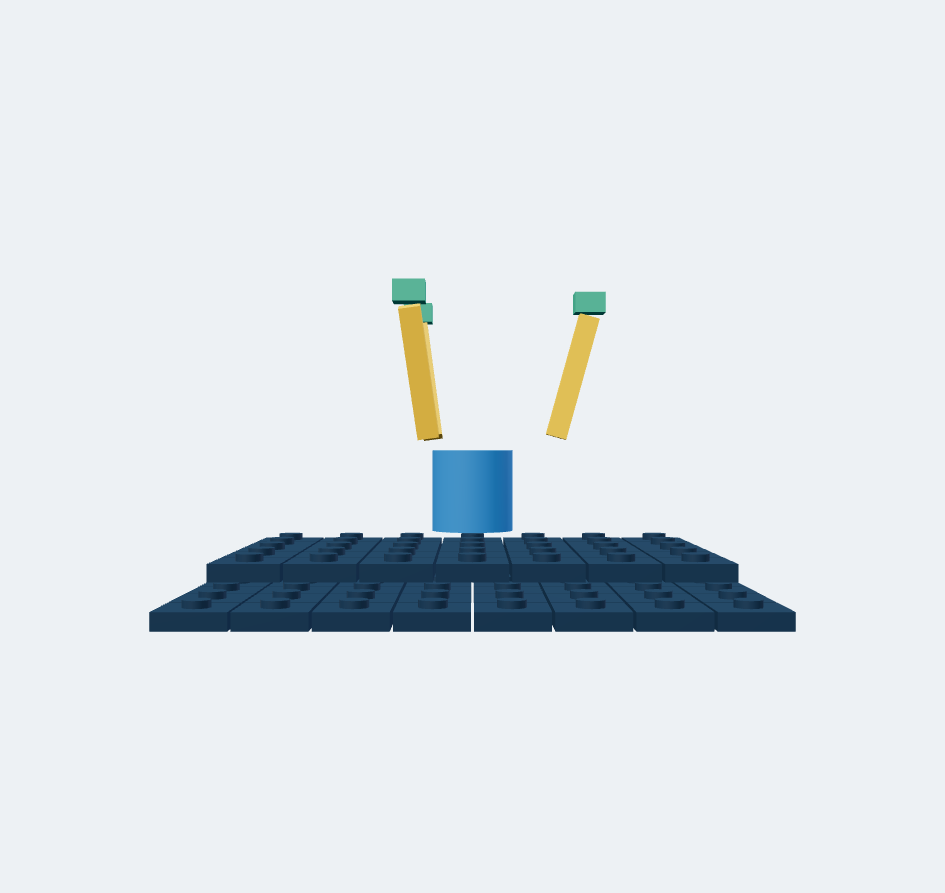
\includegraphics[width=.24\textwidth]{figures/hierarchy-expanded/exp-d1-gripper-2-front.png}
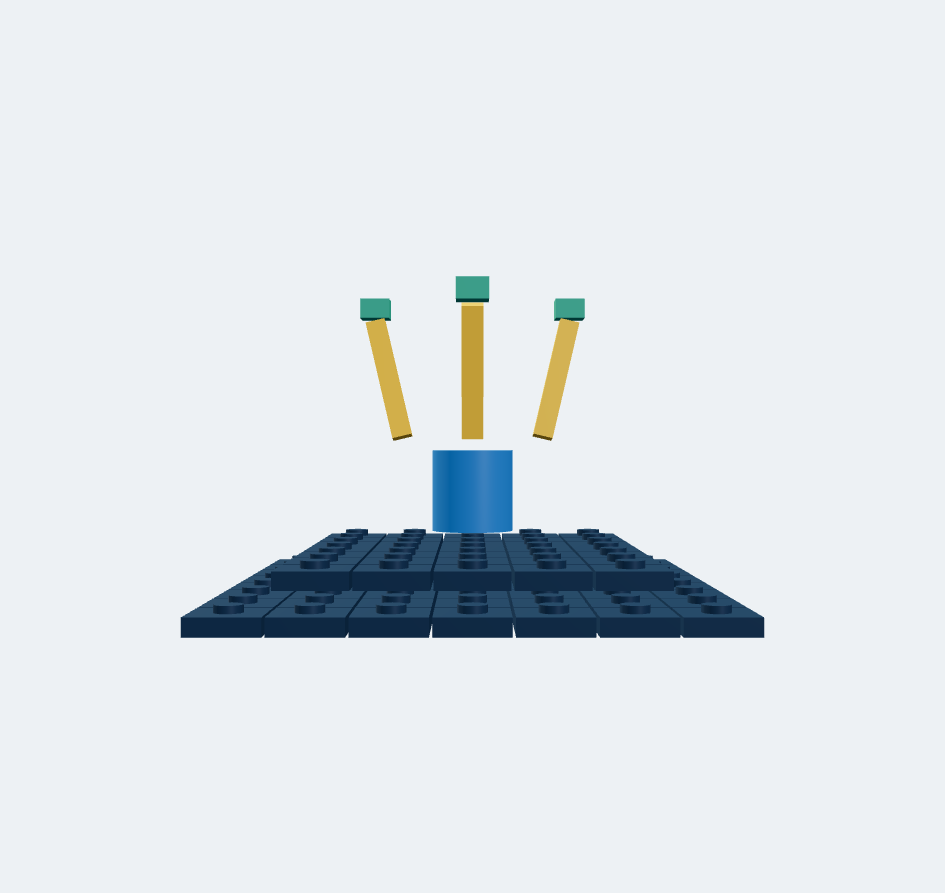
\includegraphics[width=.24\textwidth]{figures/hierarchy-expanded/exp-d1-gripper-2-side.png}
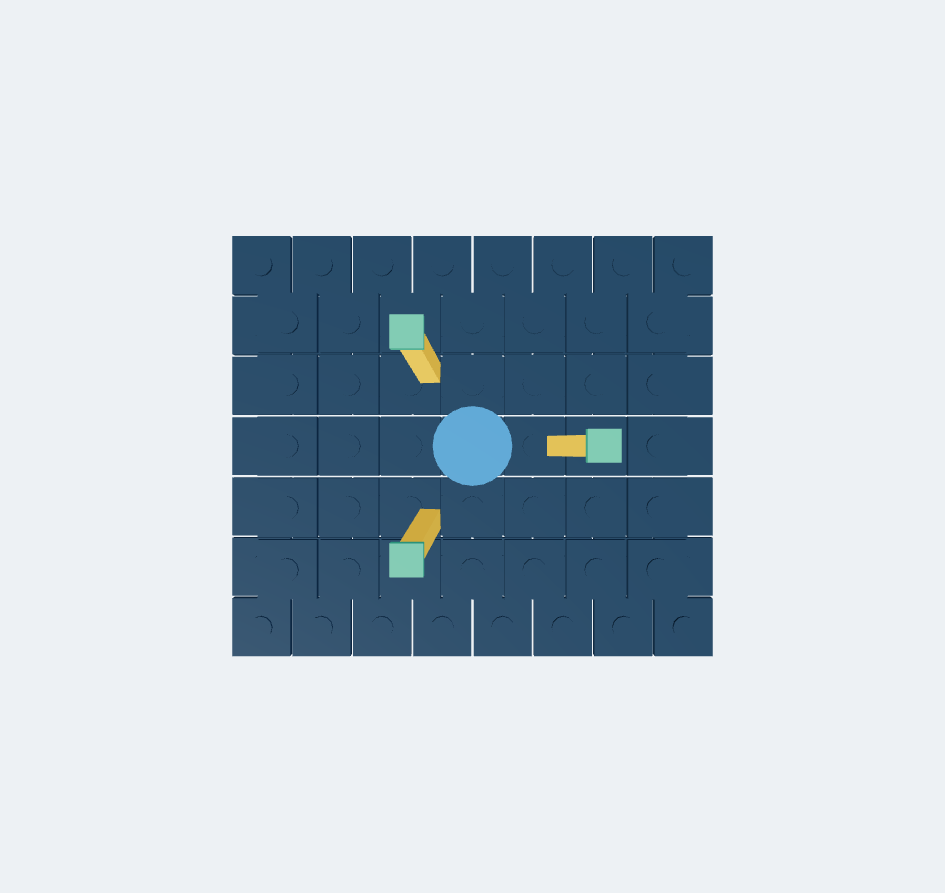
\includegraphics[width=.24\textwidth]{figures/hierarchy-expanded/exp-d1-gripper-2-top.png}
\end{center}
\noindent All 48 families share this source. Full inputs and answers appear in the companion question bank.
\begin{center}\tiny\begin{tabular}{rllll}\toprule No. & Family & Layer & Output & Evidence\\\midrule
1 & identify & atomic & single-choice & model-state \\
2 & count & atomic & single-choice & model-state \\
3 & color & atomic & single-choice & model-state \\
4 & position & atomic & single-choice & model-state \\
5 & joint-type & atomic & single-choice & model-state \\
6 & parent & atomic & single-choice & model-state \\
7 & anchor & atomic & single-choice & model-state \\
8 & degree & atomic & single-choice & model-state \\
9 & recolor & atomic & single-choice & model-state \\
10 & add & atomic & single-choice & model-state \\
11 & remove & atomic & single-choice & model-state \\
12 & replace & atomic & single-choice & model-state \\
13 & translate & atomic & single-choice & model-state \\
14 & rotate & atomic & single-choice & model-state \\
15 & next-module & atomic & single-choice & model-state \\
16 & inventory & atomic & single-choice & model-state \\
17 & boundary & atomic & single-choice & model-state \\
18 & no-op & atomic & single-choice & model-state \\
19 & prefix & metacognitive & single-choice & support-graph \\
20 & access & metacognitive & multiple-choice & Rapier \\
21 & counterfactual & metacognitive & single-choice & support-graph \\
22 & dynamic & metacognitive & single-choice & Rapier \\
23 & kinematic & metacognitive & multiple-choice & model-state \\
24 & diagnosis & metacognitive & multiple-choice & model-state \\
25 & information-gain & metacognitive & multiple-choice & finite-world \\
26 & abstention & metacognitive & single-choice & finite-world \\
27 & posterior & metacognitive & single-choice & finite-world \\
28 & pareto & metacognitive & multiple-choice & model-state \\
29 & assembly & procedural & actions & state-machine \\
30 & disassembly & procedural & actions & state-machine \\
31 & service-repair & procedural & actions & state-machine \\
32 & compound-edit & procedural & actions & state-machine \\
33 & multi-fault & integrative & actions & state-machine \\
34 & scheduling & integrative & schedule & resource-schedule \\
35 & policy & integrative & policy & finite-world \\
36 & local-frame & atomic & single-choice & model-state \\
37 & projection & atomic & single-choice & model-state \\
38 & relative-order & atomic & single-choice & model-state \\
39 & joint-axis & atomic & single-choice & model-state \\
40 & clearance-margin & metacognitive & single-choice & model-state \\
41 & load-moment & metacognitive & single-choice & model-state \\
42 & weighted-posterior & metacognitive & single-choice & finite-world \\
43 & expected-loss & metacognitive & single-choice & finite-world \\
44 & trace-threshold & metacognitive & single-choice & Rapier \\
45 & guarded-repair & procedural & actions & state-machine \\
46 & rollback & procedural & actions & state-machine \\
47 & resource-repair & integrative & actions & state-machine \\
48 & budget-policy & integrative & policy & finite-world \\
\bottomrule\end{tabular}\end{center}
\clearpage
\subsection{16. Inclined Probe Stand (D1)}
91 visible parts; 4 modules; 3 joints. Representative-point motion 0.0000; rotation 0.0000 rad.
\begin{center}
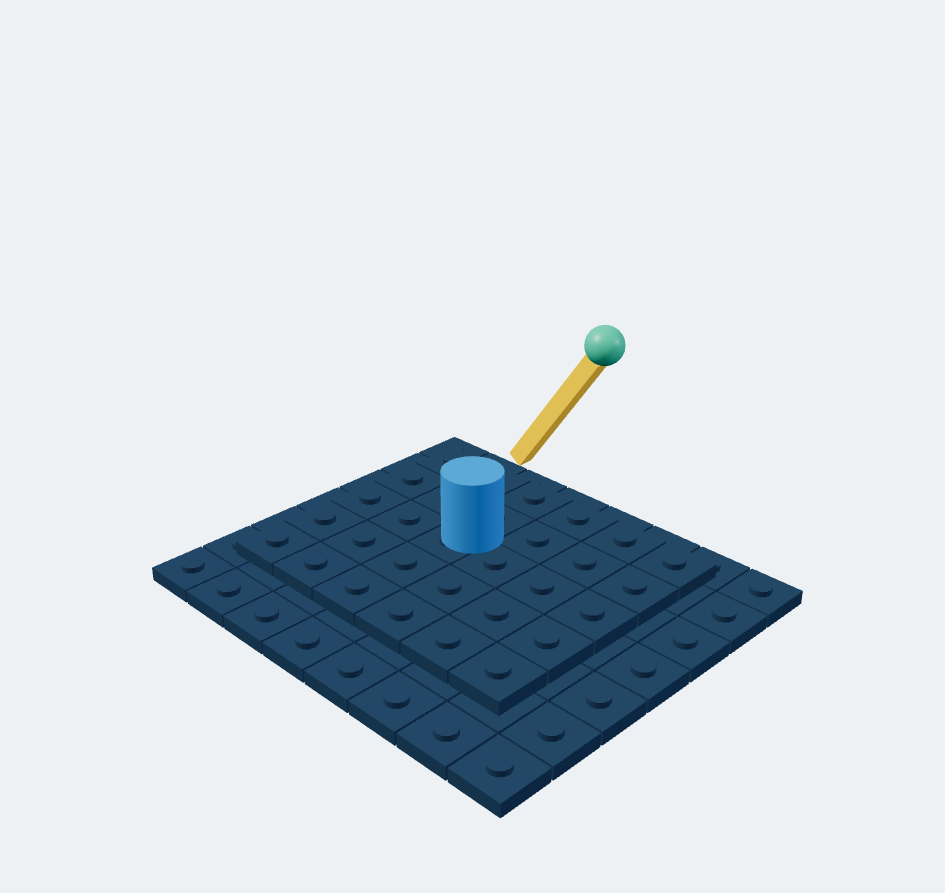
\includegraphics[width=.24\textwidth]{figures/hierarchy-expanded/exp-d1-probe-1-iso.png}
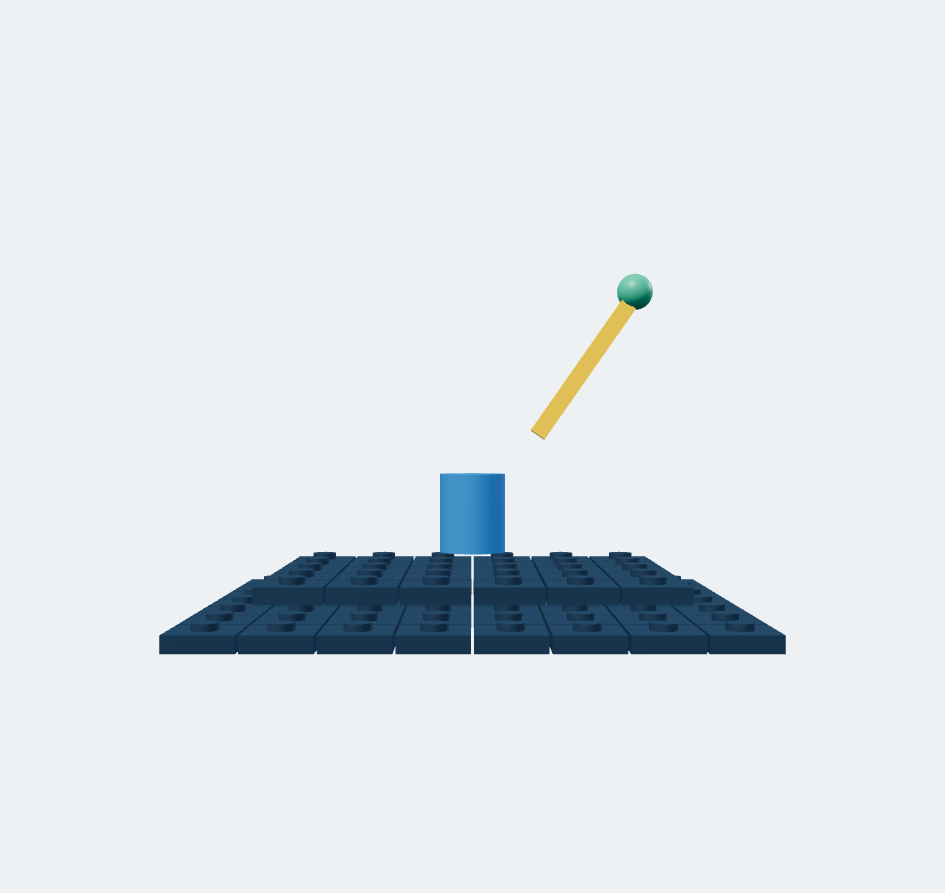
\includegraphics[width=.24\textwidth]{figures/hierarchy-expanded/exp-d1-probe-1-front.png}
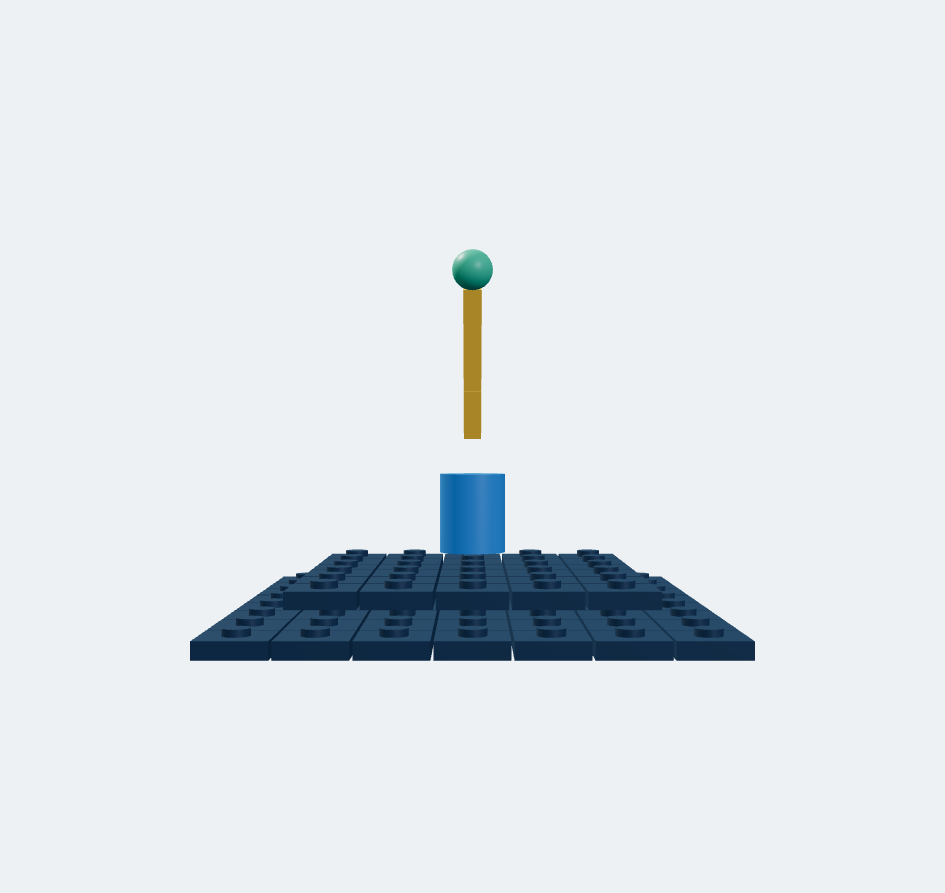
\includegraphics[width=.24\textwidth]{figures/hierarchy-expanded/exp-d1-probe-1-side.png}
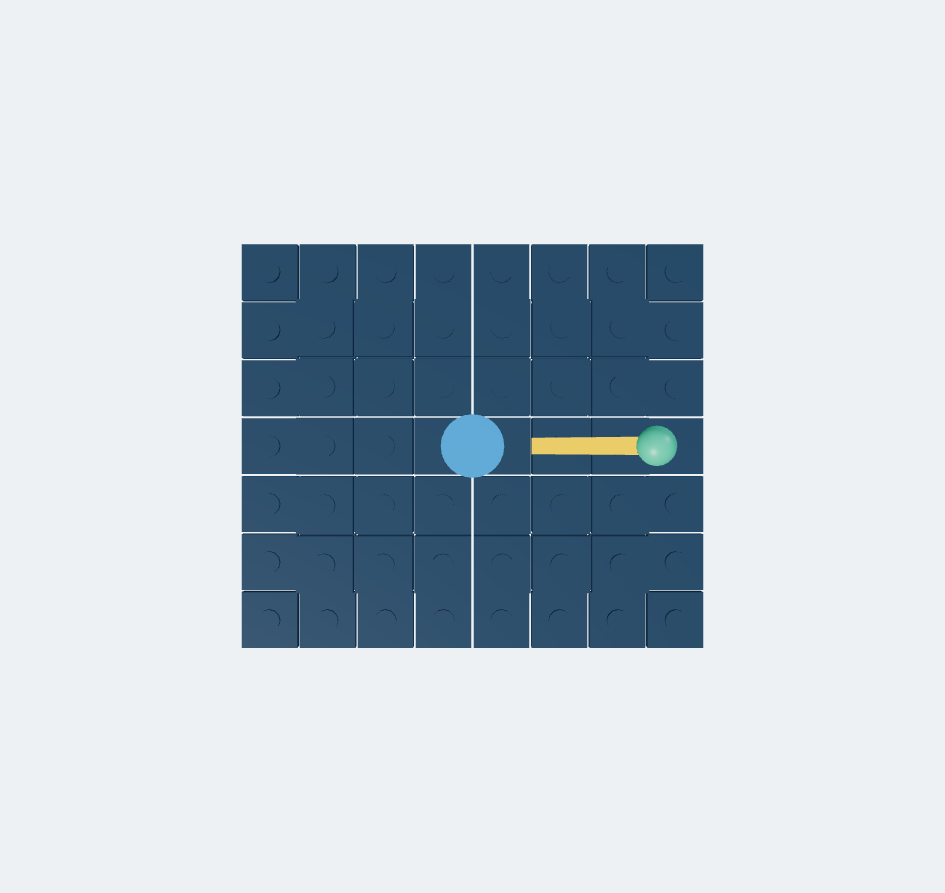
\includegraphics[width=.24\textwidth]{figures/hierarchy-expanded/exp-d1-probe-1-top.png}
\end{center}
\noindent All 48 families share this source. Full inputs and answers appear in the companion question bank.
\begin{center}\tiny\begin{tabular}{rllll}\toprule No. & Family & Layer & Output & Evidence\\\midrule
1 & identify & atomic & single-choice & model-state \\
2 & count & atomic & single-choice & model-state \\
3 & color & atomic & single-choice & model-state \\
4 & position & atomic & single-choice & model-state \\
5 & joint-type & atomic & single-choice & model-state \\
6 & parent & atomic & single-choice & model-state \\
7 & anchor & atomic & single-choice & model-state \\
8 & degree & atomic & single-choice & model-state \\
9 & recolor & atomic & single-choice & model-state \\
10 & add & atomic & single-choice & model-state \\
11 & remove & atomic & single-choice & model-state \\
12 & replace & atomic & single-choice & model-state \\
13 & translate & atomic & single-choice & model-state \\
14 & rotate & atomic & single-choice & model-state \\
15 & next-module & atomic & single-choice & model-state \\
16 & inventory & atomic & single-choice & model-state \\
17 & boundary & atomic & single-choice & model-state \\
18 & no-op & atomic & single-choice & model-state \\
19 & prefix & metacognitive & single-choice & support-graph \\
20 & access & metacognitive & multiple-choice & Rapier \\
21 & counterfactual & metacognitive & single-choice & support-graph \\
22 & dynamic & metacognitive & single-choice & Rapier \\
23 & kinematic & metacognitive & multiple-choice & model-state \\
24 & diagnosis & metacognitive & multiple-choice & model-state \\
25 & information-gain & metacognitive & multiple-choice & finite-world \\
26 & abstention & metacognitive & single-choice & finite-world \\
27 & posterior & metacognitive & single-choice & finite-world \\
28 & pareto & metacognitive & multiple-choice & model-state \\
29 & assembly & procedural & actions & state-machine \\
30 & disassembly & procedural & actions & state-machine \\
31 & service-repair & procedural & actions & state-machine \\
32 & compound-edit & procedural & actions & state-machine \\
33 & multi-fault & integrative & actions & state-machine \\
34 & scheduling & integrative & schedule & resource-schedule \\
35 & policy & integrative & policy & finite-world \\
36 & local-frame & atomic & single-choice & model-state \\
37 & projection & atomic & single-choice & model-state \\
38 & relative-order & atomic & single-choice & model-state \\
39 & joint-axis & atomic & single-choice & model-state \\
40 & clearance-margin & metacognitive & single-choice & model-state \\
41 & load-moment & metacognitive & single-choice & model-state \\
42 & weighted-posterior & metacognitive & single-choice & finite-world \\
43 & expected-loss & metacognitive & single-choice & finite-world \\
44 & trace-threshold & metacognitive & single-choice & Rapier \\
45 & guarded-repair & procedural & actions & state-machine \\
46 & rollback & procedural & actions & state-machine \\
47 & resource-repair & integrative & actions & state-machine \\
48 & budget-policy & integrative & policy & finite-world \\
\bottomrule\end{tabular}\end{center}
\clearpage
\subsection{17. Three-direction Probe Stand (D1)}
104 visible parts; 6 modules; 5 joints. Representative-point motion 0.0000; rotation 0.0000 rad.
\begin{center}
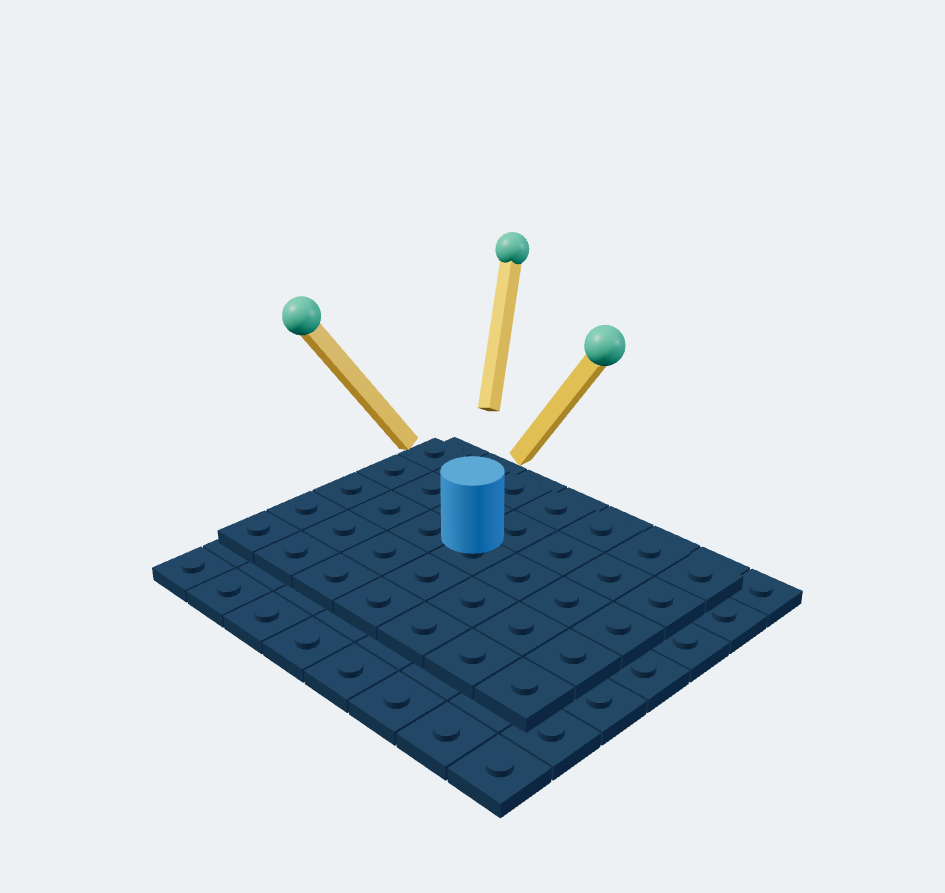
\includegraphics[width=.24\textwidth]{figures/hierarchy-expanded/exp-d1-probe-2-iso.png}
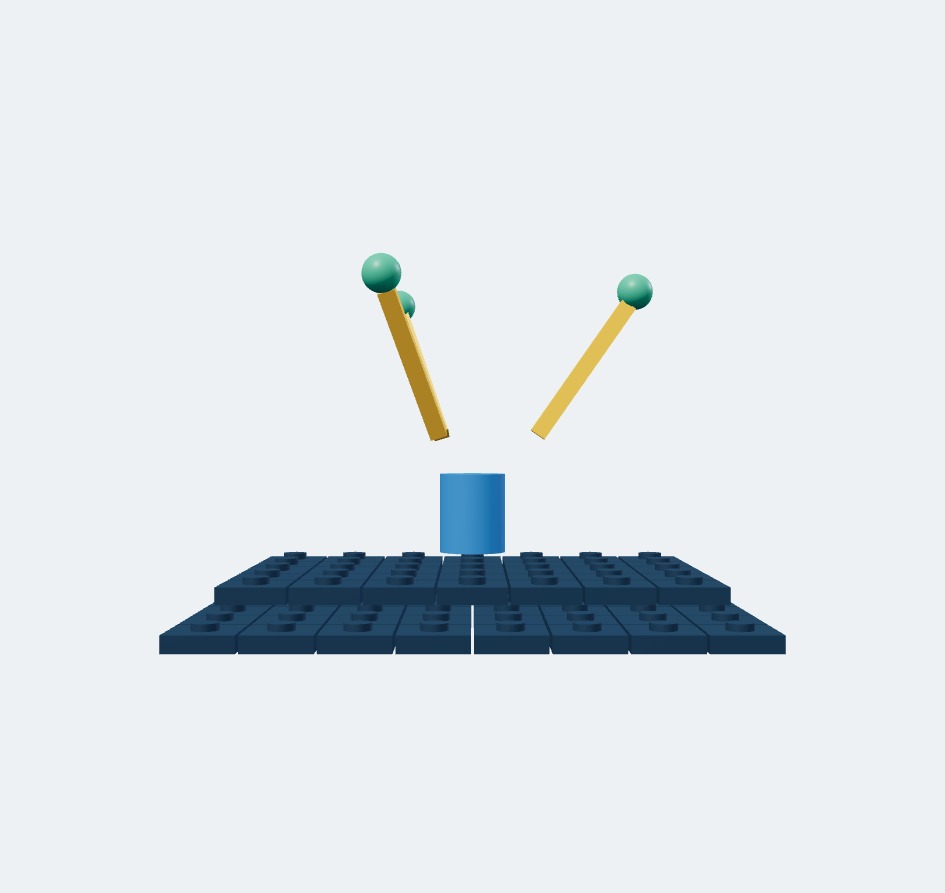
\includegraphics[width=.24\textwidth]{figures/hierarchy-expanded/exp-d1-probe-2-front.png}
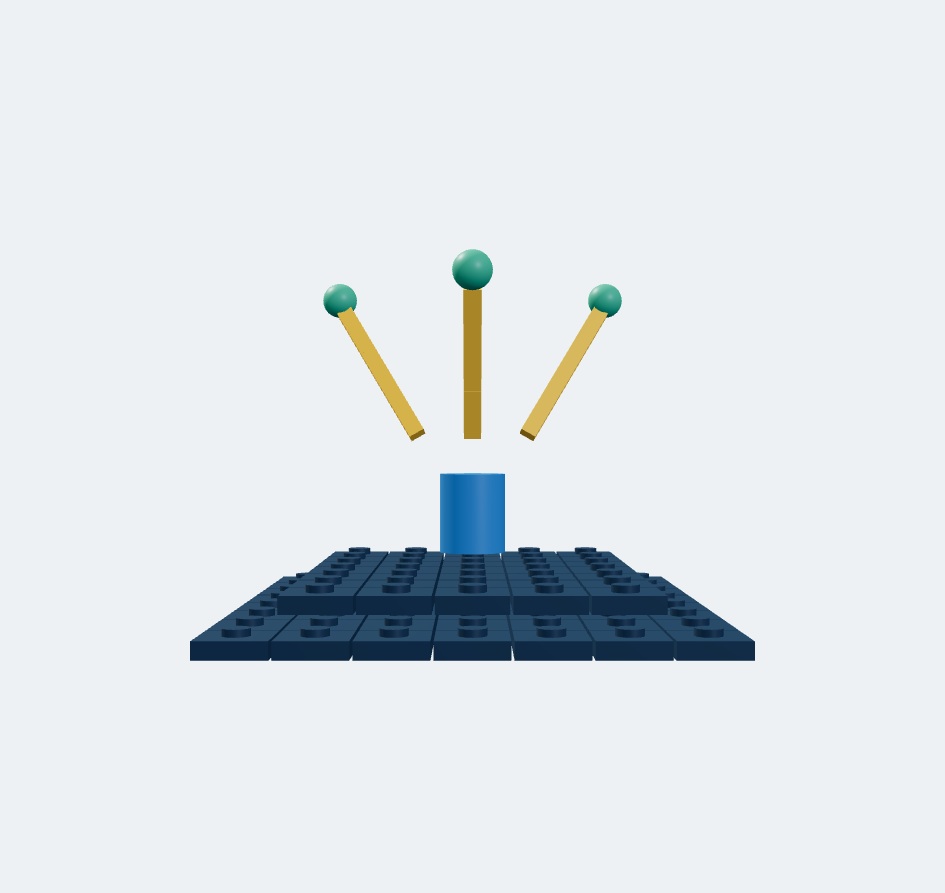
\includegraphics[width=.24\textwidth]{figures/hierarchy-expanded/exp-d1-probe-2-side.png}
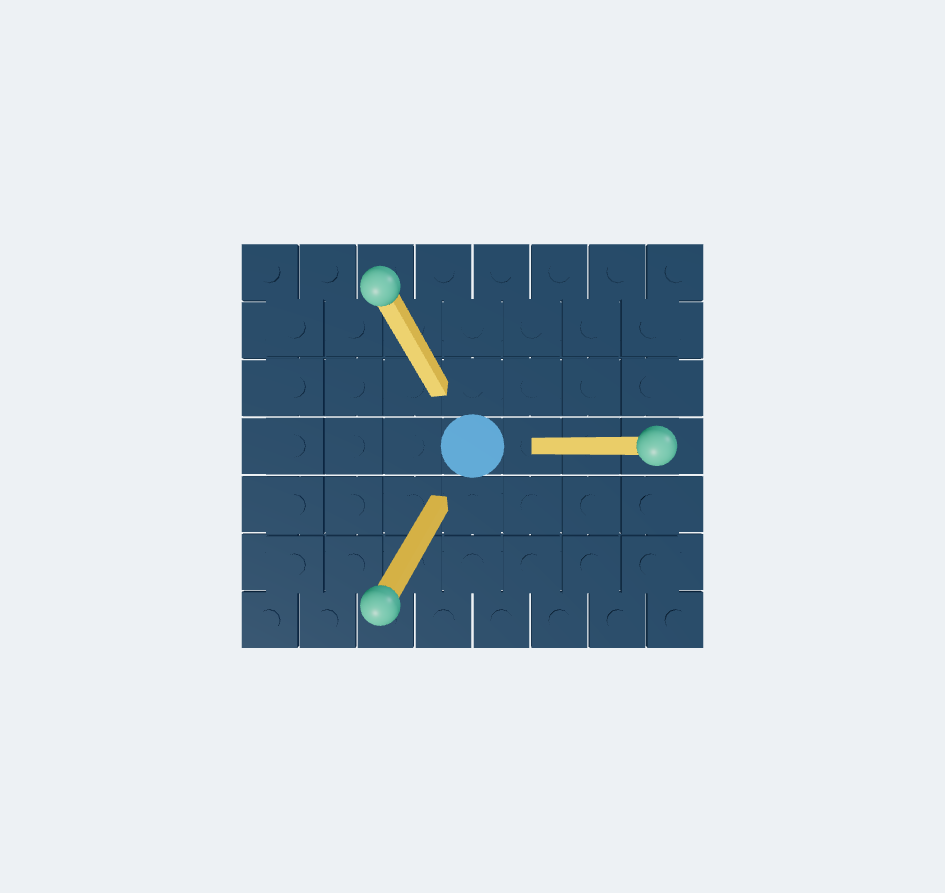
\includegraphics[width=.24\textwidth]{figures/hierarchy-expanded/exp-d1-probe-2-top.png}
\end{center}
\noindent All 48 families share this source. Full inputs and answers appear in the companion question bank.
\begin{center}\tiny\begin{tabular}{rllll}\toprule No. & Family & Layer & Output & Evidence\\\midrule
1 & identify & atomic & single-choice & model-state \\
2 & count & atomic & single-choice & model-state \\
3 & color & atomic & single-choice & model-state \\
4 & position & atomic & single-choice & model-state \\
5 & joint-type & atomic & single-choice & model-state \\
6 & parent & atomic & single-choice & model-state \\
7 & anchor & atomic & single-choice & model-state \\
8 & degree & atomic & single-choice & model-state \\
9 & recolor & atomic & single-choice & model-state \\
10 & add & atomic & single-choice & model-state \\
11 & remove & atomic & single-choice & model-state \\
12 & replace & atomic & single-choice & model-state \\
13 & translate & atomic & single-choice & model-state \\
14 & rotate & atomic & single-choice & model-state \\
15 & next-module & atomic & single-choice & model-state \\
16 & inventory & atomic & single-choice & model-state \\
17 & boundary & atomic & single-choice & model-state \\
18 & no-op & atomic & single-choice & model-state \\
19 & prefix & metacognitive & single-choice & support-graph \\
20 & access & metacognitive & multiple-choice & Rapier \\
21 & counterfactual & metacognitive & single-choice & support-graph \\
22 & dynamic & metacognitive & single-choice & Rapier \\
23 & kinematic & metacognitive & multiple-choice & model-state \\
24 & diagnosis & metacognitive & multiple-choice & model-state \\
25 & information-gain & metacognitive & multiple-choice & finite-world \\
26 & abstention & metacognitive & single-choice & finite-world \\
27 & posterior & metacognitive & single-choice & finite-world \\
28 & pareto & metacognitive & multiple-choice & model-state \\
29 & assembly & procedural & actions & state-machine \\
30 & disassembly & procedural & actions & state-machine \\
31 & service-repair & procedural & actions & state-machine \\
32 & compound-edit & procedural & actions & state-machine \\
33 & multi-fault & integrative & actions & state-machine \\
34 & scheduling & integrative & schedule & resource-schedule \\
35 & policy & integrative & policy & finite-world \\
36 & local-frame & atomic & single-choice & model-state \\
37 & projection & atomic & single-choice & model-state \\
38 & relative-order & atomic & single-choice & model-state \\
39 & joint-axis & atomic & single-choice & model-state \\
40 & clearance-margin & metacognitive & single-choice & model-state \\
41 & load-moment & metacognitive & single-choice & model-state \\
42 & weighted-posterior & metacognitive & single-choice & finite-world \\
43 & expected-loss & metacognitive & single-choice & finite-world \\
44 & trace-threshold & metacognitive & single-choice & Rapier \\
45 & guarded-repair & procedural & actions & state-machine \\
46 & rollback & procedural & actions & state-machine \\
47 & resource-repair & integrative & actions & state-machine \\
48 & budget-policy & integrative & policy & finite-world \\
\bottomrule\end{tabular}\end{center}
\clearpage
\subsection{18. Cross-feed Stage (D1)}
108 visible parts; 4 modules; 3 joints. Representative-point motion 0.0000; rotation 0.0000 rad.
\begin{center}
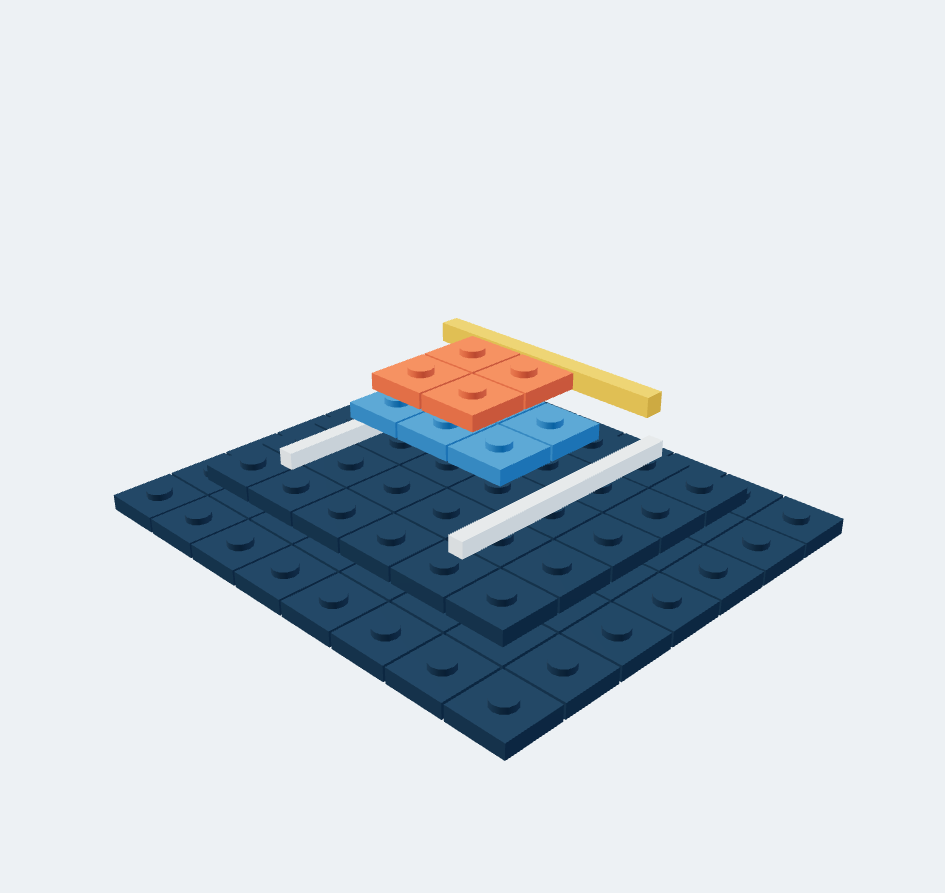
\includegraphics[width=.24\textwidth]{figures/hierarchy-expanded/exp-d1-slide-1-iso.png}
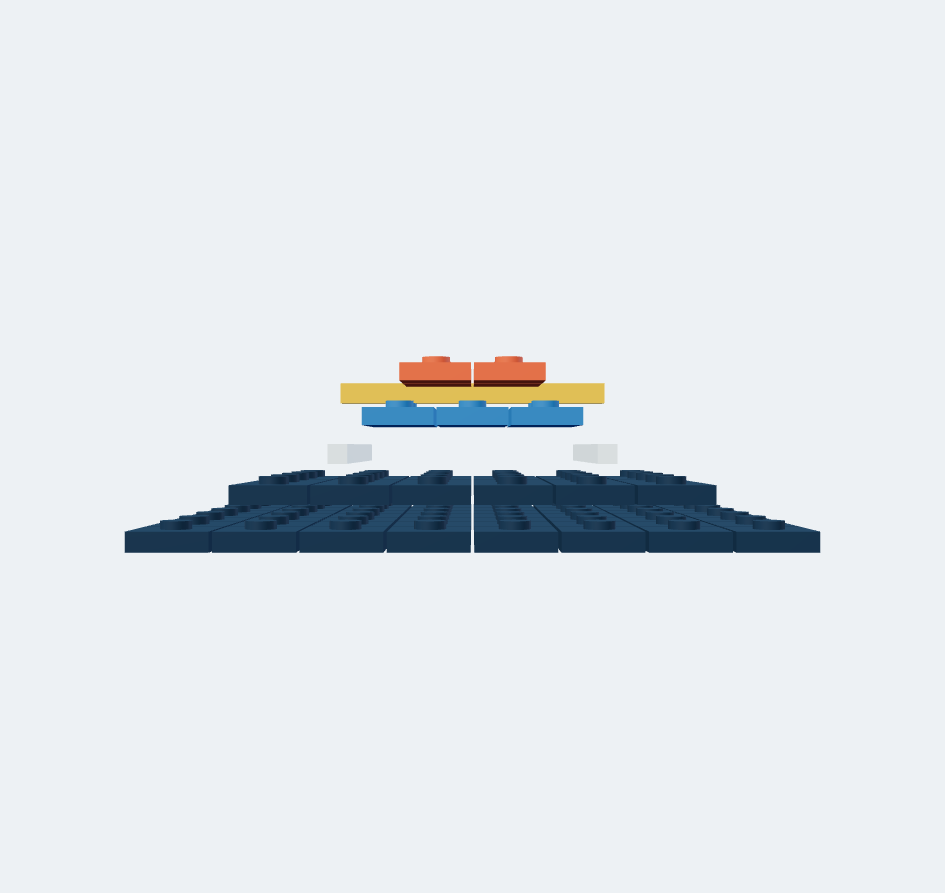
\includegraphics[width=.24\textwidth]{figures/hierarchy-expanded/exp-d1-slide-1-front.png}
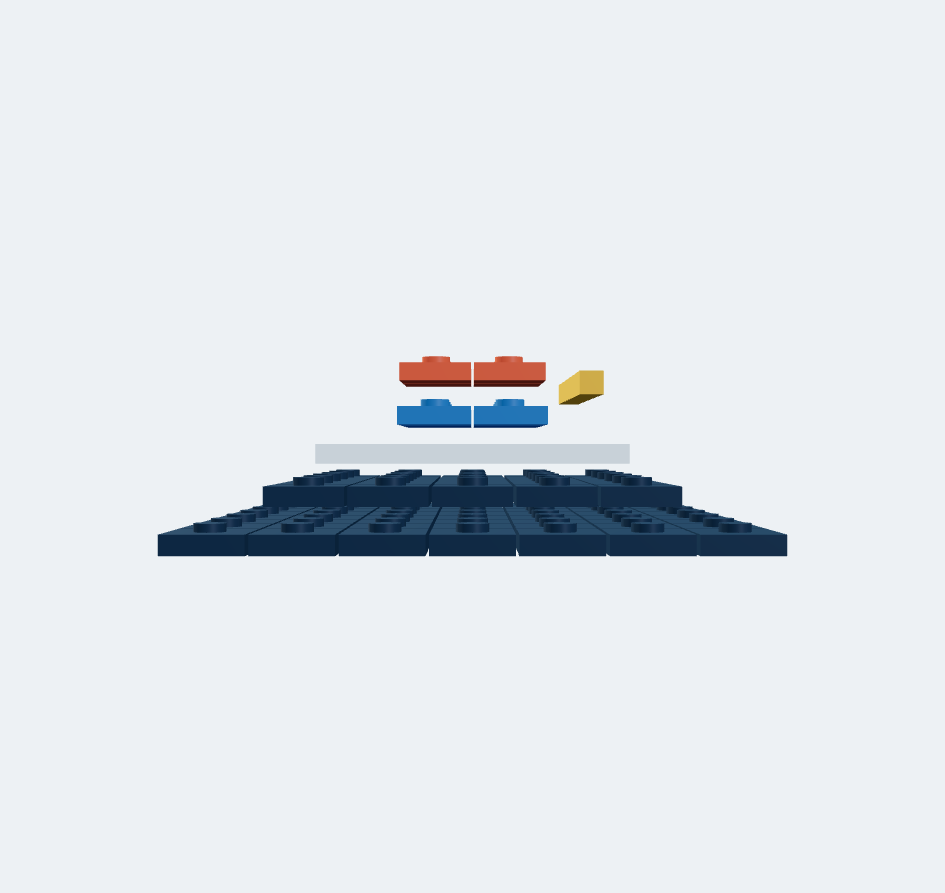
\includegraphics[width=.24\textwidth]{figures/hierarchy-expanded/exp-d1-slide-1-side.png}
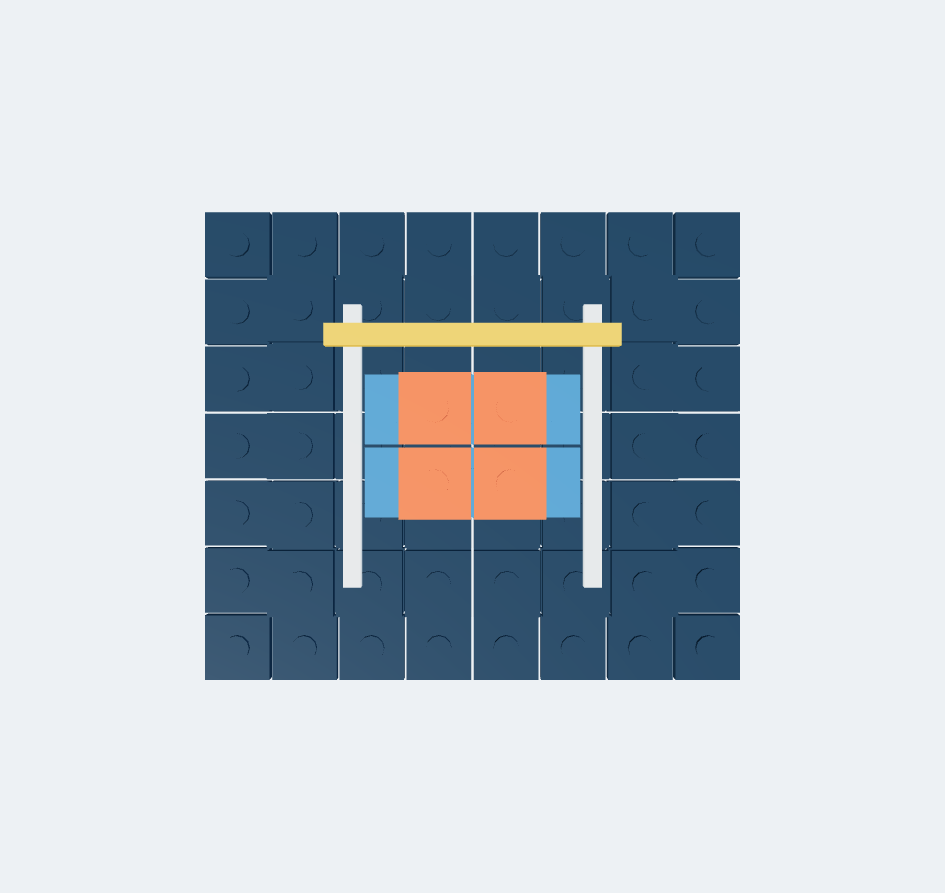
\includegraphics[width=.24\textwidth]{figures/hierarchy-expanded/exp-d1-slide-1-top.png}
\end{center}
\noindent All 48 families share this source. Full inputs and answers appear in the companion question bank.
\begin{center}\tiny\begin{tabular}{rllll}\toprule No. & Family & Layer & Output & Evidence\\\midrule
1 & identify & atomic & single-choice & model-state \\
2 & count & atomic & single-choice & model-state \\
3 & color & atomic & single-choice & model-state \\
4 & position & atomic & single-choice & model-state \\
5 & joint-type & atomic & single-choice & model-state \\
6 & parent & atomic & single-choice & model-state \\
7 & anchor & atomic & single-choice & model-state \\
8 & degree & atomic & single-choice & model-state \\
9 & recolor & atomic & single-choice & model-state \\
10 & add & atomic & single-choice & model-state \\
11 & remove & atomic & single-choice & model-state \\
12 & replace & atomic & single-choice & model-state \\
13 & translate & atomic & single-choice & model-state \\
14 & rotate & atomic & single-choice & model-state \\
15 & next-module & atomic & single-choice & model-state \\
16 & inventory & atomic & single-choice & model-state \\
17 & boundary & atomic & single-choice & model-state \\
18 & no-op & atomic & single-choice & model-state \\
19 & prefix & metacognitive & single-choice & support-graph \\
20 & access & metacognitive & multiple-choice & Rapier \\
21 & counterfactual & metacognitive & single-choice & support-graph \\
22 & dynamic & metacognitive & single-choice & Rapier \\
23 & kinematic & metacognitive & multiple-choice & model-state \\
24 & diagnosis & metacognitive & multiple-choice & model-state \\
25 & information-gain & metacognitive & multiple-choice & finite-world \\
26 & abstention & metacognitive & single-choice & finite-world \\
27 & posterior & metacognitive & single-choice & finite-world \\
28 & pareto & metacognitive & multiple-choice & model-state \\
29 & assembly & procedural & actions & state-machine \\
30 & disassembly & procedural & actions & state-machine \\
31 & service-repair & procedural & actions & state-machine \\
32 & compound-edit & procedural & actions & state-machine \\
33 & multi-fault & integrative & actions & state-machine \\
34 & scheduling & integrative & schedule & resource-schedule \\
35 & policy & integrative & policy & finite-world \\
36 & local-frame & atomic & single-choice & model-state \\
37 & projection & atomic & single-choice & model-state \\
38 & relative-order & atomic & single-choice & model-state \\
39 & joint-axis & atomic & single-choice & model-state \\
40 & clearance-margin & metacognitive & single-choice & model-state \\
41 & load-moment & metacognitive & single-choice & model-state \\
42 & weighted-posterior & metacognitive & single-choice & finite-world \\
43 & expected-loss & metacognitive & single-choice & finite-world \\
44 & trace-threshold & metacognitive & single-choice & Rapier \\
45 & guarded-repair & procedural & actions & state-machine \\
46 & rollback & procedural & actions & state-machine \\
47 & resource-repair & integrative & actions & state-machine \\
48 & budget-policy & integrative & policy & finite-world \\
\bottomrule\end{tabular}\end{center}
\clearpage
\subsection{19. Twin-rail Elevator (D1)}
113 visible parts; 4 modules; 3 joints. Representative-point motion 0.0002; rotation 0.0000 rad.
\begin{center}
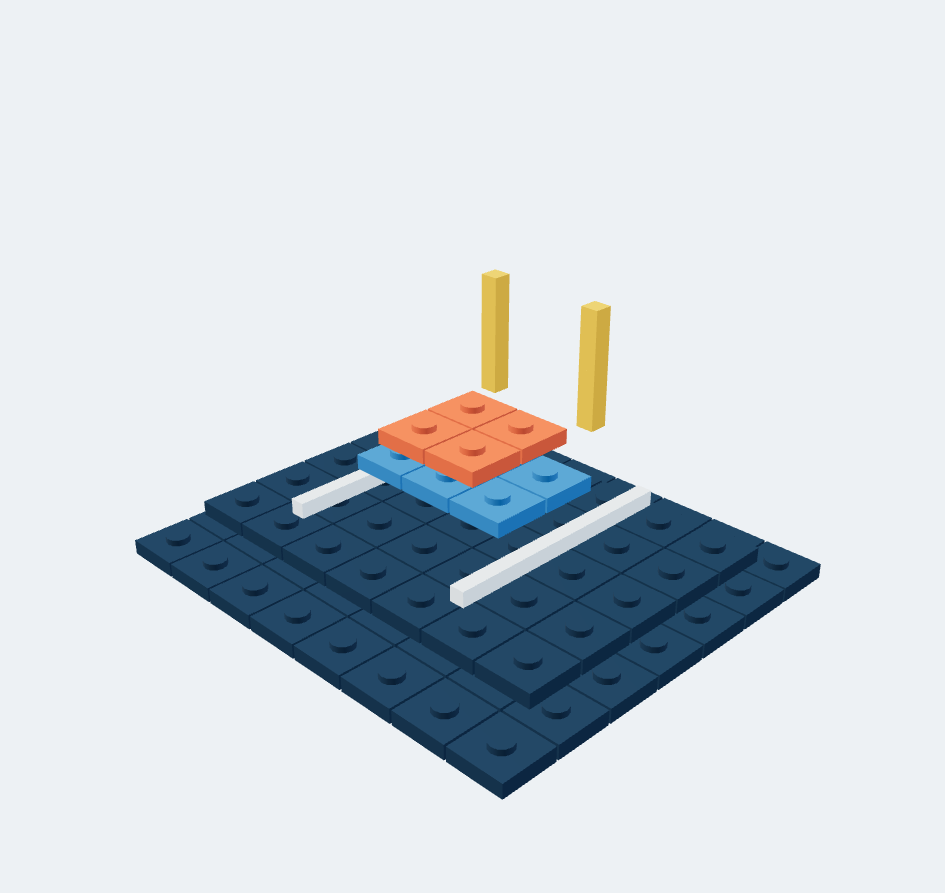
\includegraphics[width=.24\textwidth]{figures/hierarchy-expanded/exp-d1-slide-2-iso.png}
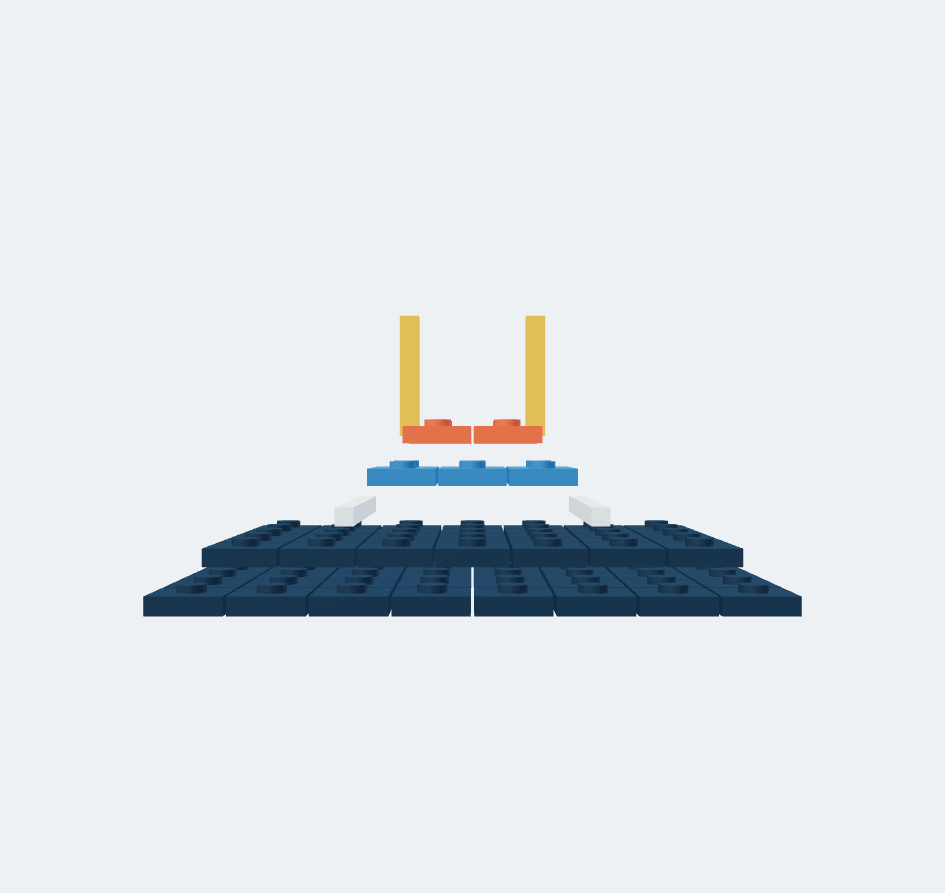
\includegraphics[width=.24\textwidth]{figures/hierarchy-expanded/exp-d1-slide-2-front.png}
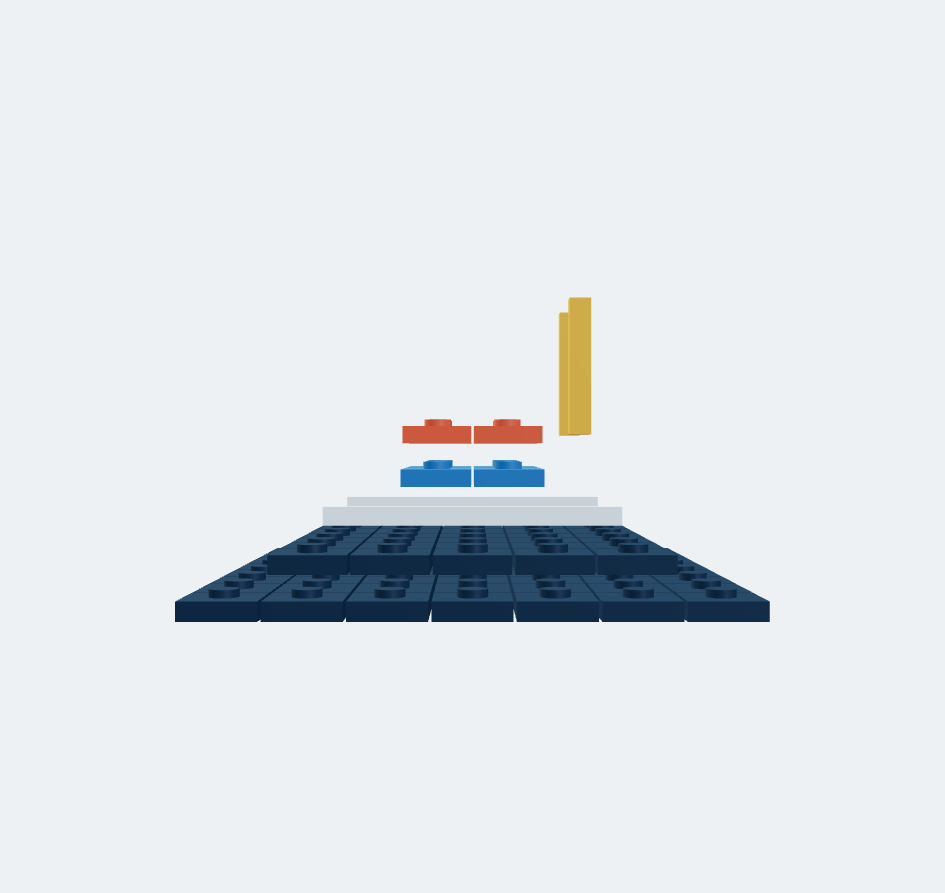
\includegraphics[width=.24\textwidth]{figures/hierarchy-expanded/exp-d1-slide-2-side.png}
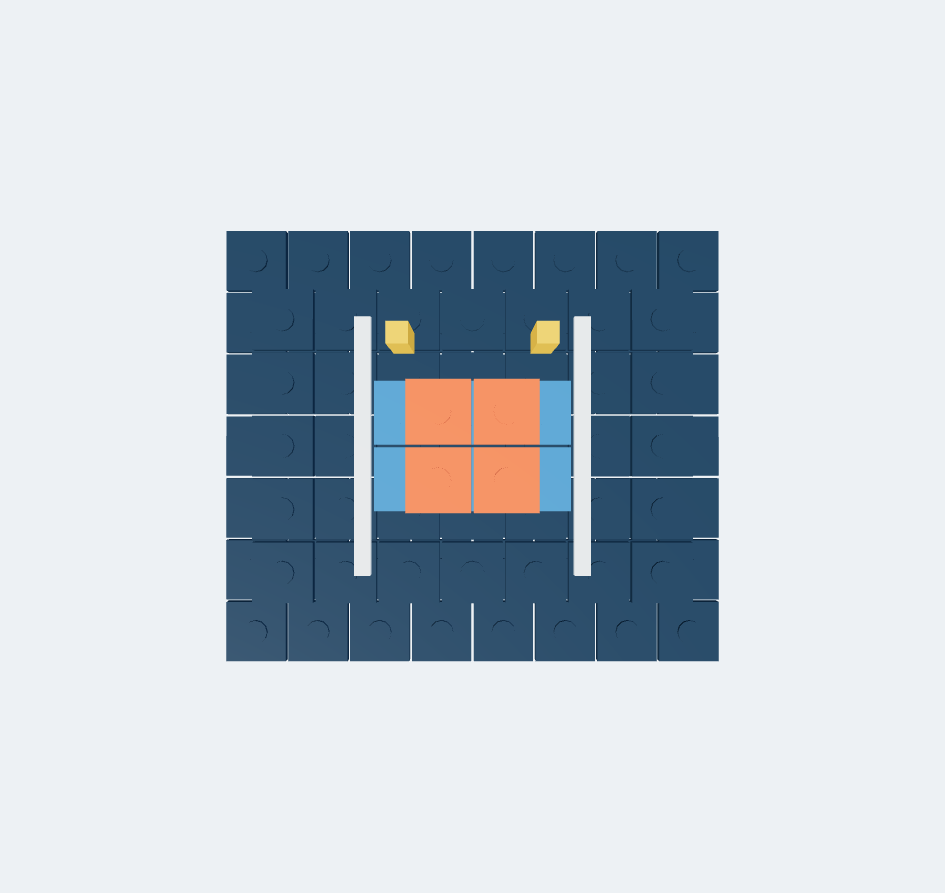
\includegraphics[width=.24\textwidth]{figures/hierarchy-expanded/exp-d1-slide-2-top.png}
\end{center}
\noindent All 48 families share this source. Full inputs and answers appear in the companion question bank.
\begin{center}\tiny\begin{tabular}{rllll}\toprule No. & Family & Layer & Output & Evidence\\\midrule
1 & identify & atomic & single-choice & model-state \\
2 & count & atomic & single-choice & model-state \\
3 & color & atomic & single-choice & model-state \\
4 & position & atomic & single-choice & model-state \\
5 & joint-type & atomic & single-choice & model-state \\
6 & parent & atomic & single-choice & model-state \\
7 & anchor & atomic & single-choice & model-state \\
8 & degree & atomic & single-choice & model-state \\
9 & recolor & atomic & single-choice & model-state \\
10 & add & atomic & single-choice & model-state \\
11 & remove & atomic & single-choice & model-state \\
12 & replace & atomic & single-choice & model-state \\
13 & translate & atomic & single-choice & model-state \\
14 & rotate & atomic & single-choice & model-state \\
15 & next-module & atomic & single-choice & model-state \\
16 & inventory & atomic & single-choice & model-state \\
17 & boundary & atomic & single-choice & model-state \\
18 & no-op & atomic & single-choice & model-state \\
19 & prefix & metacognitive & single-choice & support-graph \\
20 & access & metacognitive & multiple-choice & Rapier \\
21 & counterfactual & metacognitive & single-choice & support-graph \\
22 & dynamic & metacognitive & single-choice & Rapier \\
23 & kinematic & metacognitive & multiple-choice & model-state \\
24 & diagnosis & metacognitive & multiple-choice & model-state \\
25 & information-gain & metacognitive & multiple-choice & finite-world \\
26 & abstention & metacognitive & single-choice & finite-world \\
27 & posterior & metacognitive & single-choice & finite-world \\
28 & pareto & metacognitive & multiple-choice & model-state \\
29 & assembly & procedural & actions & state-machine \\
30 & disassembly & procedural & actions & state-machine \\
31 & service-repair & procedural & actions & state-machine \\
32 & compound-edit & procedural & actions & state-machine \\
33 & multi-fault & integrative & actions & state-machine \\
34 & scheduling & integrative & schedule & resource-schedule \\
35 & policy & integrative & policy & finite-world \\
36 & local-frame & atomic & single-choice & model-state \\
37 & projection & atomic & single-choice & model-state \\
38 & relative-order & atomic & single-choice & model-state \\
39 & joint-axis & atomic & single-choice & model-state \\
40 & clearance-margin & metacognitive & single-choice & model-state \\
41 & load-moment & metacognitive & single-choice & model-state \\
42 & weighted-posterior & metacognitive & single-choice & finite-world \\
43 & expected-loss & metacognitive & single-choice & finite-world \\
44 & trace-threshold & metacognitive & single-choice & Rapier \\
45 & guarded-repair & procedural & actions & state-machine \\
46 & rollback & procedural & actions & state-machine \\
47 & resource-repair & integrative & actions & state-machine \\
48 & budget-policy & integrative & policy & finite-world \\
\bottomrule\end{tabular}\end{center}
\clearpage
\subsection{20. Three-point Elastic Tray (D1)}
111 visible parts; 5 modules; 6 joints. Representative-point motion 0.0052; rotation 0.0035 rad.
\begin{center}
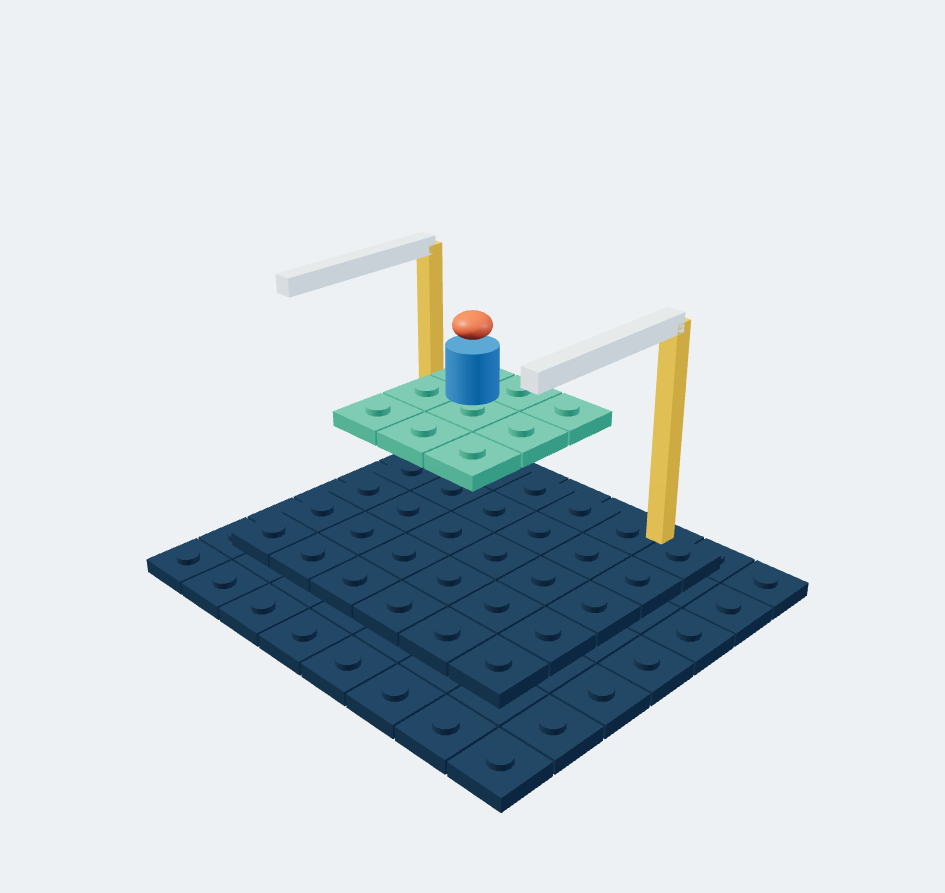
\includegraphics[width=.24\textwidth]{figures/hierarchy-expanded/exp-d1-suspension-1-iso.png}
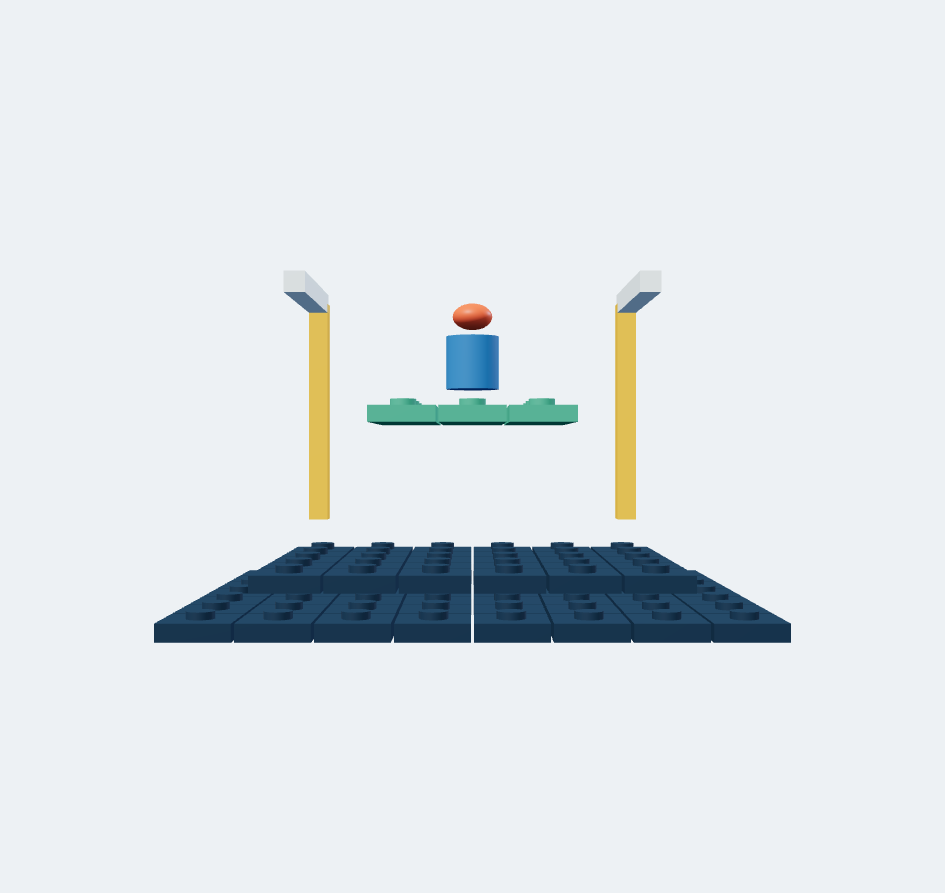
\includegraphics[width=.24\textwidth]{figures/hierarchy-expanded/exp-d1-suspension-1-front.png}
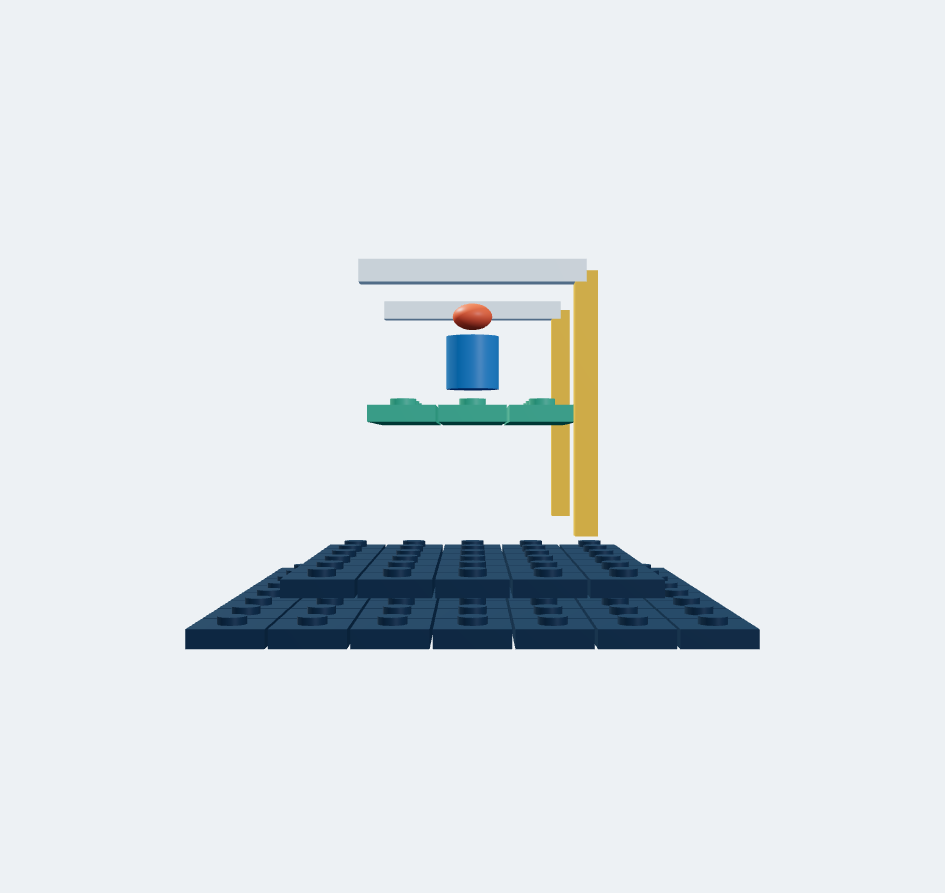
\includegraphics[width=.24\textwidth]{figures/hierarchy-expanded/exp-d1-suspension-1-side.png}
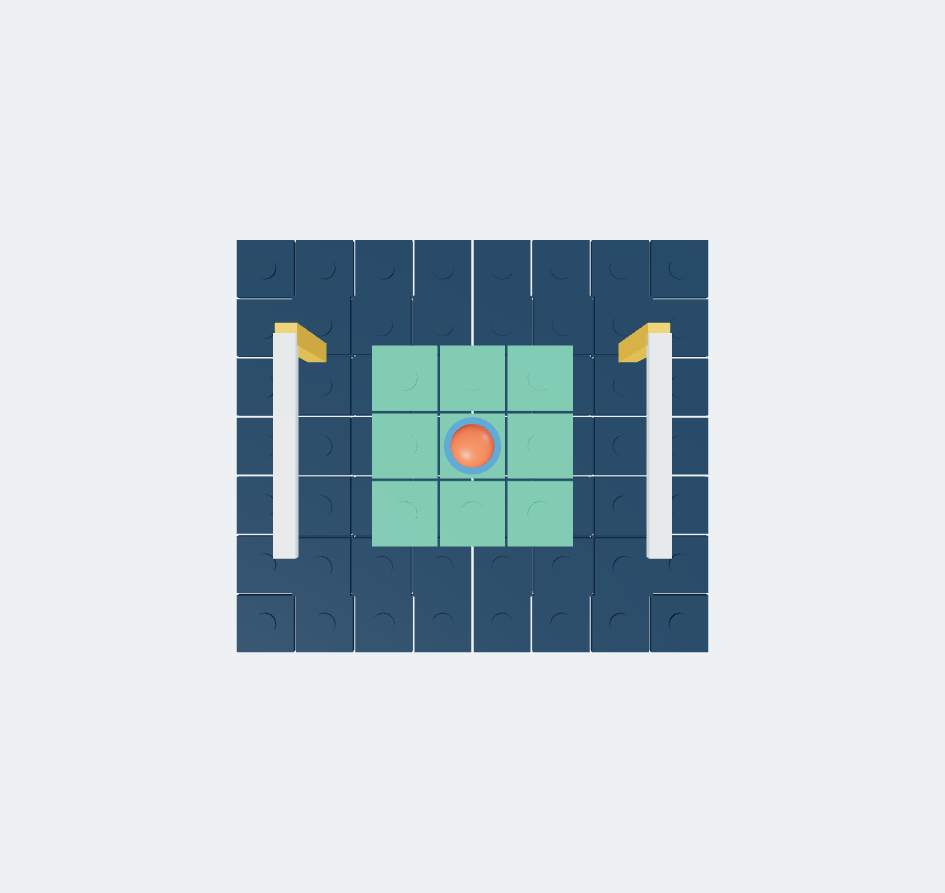
\includegraphics[width=.24\textwidth]{figures/hierarchy-expanded/exp-d1-suspension-1-top.png}
\end{center}
\noindent All 48 families share this source. Full inputs and answers appear in the companion question bank.
\begin{center}\tiny\begin{tabular}{rllll}\toprule No. & Family & Layer & Output & Evidence\\\midrule
1 & identify & atomic & single-choice & model-state \\
2 & count & atomic & single-choice & model-state \\
3 & color & atomic & single-choice & model-state \\
4 & position & atomic & single-choice & model-state \\
5 & joint-type & atomic & single-choice & model-state \\
6 & parent & atomic & single-choice & model-state \\
7 & anchor & atomic & single-choice & model-state \\
8 & degree & atomic & single-choice & model-state \\
9 & recolor & atomic & single-choice & model-state \\
10 & add & atomic & single-choice & model-state \\
11 & remove & atomic & single-choice & model-state \\
12 & replace & atomic & single-choice & model-state \\
13 & translate & atomic & single-choice & model-state \\
14 & rotate & atomic & single-choice & model-state \\
15 & next-module & atomic & single-choice & model-state \\
16 & inventory & atomic & single-choice & model-state \\
17 & boundary & atomic & single-choice & model-state \\
18 & no-op & atomic & single-choice & model-state \\
19 & prefix & metacognitive & single-choice & support-graph \\
20 & access & metacognitive & multiple-choice & Rapier \\
21 & counterfactual & metacognitive & single-choice & support-graph \\
22 & dynamic & metacognitive & single-choice & Rapier \\
23 & kinematic & metacognitive & multiple-choice & model-state \\
24 & diagnosis & metacognitive & multiple-choice & model-state \\
25 & information-gain & metacognitive & multiple-choice & finite-world \\
26 & abstention & metacognitive & single-choice & finite-world \\
27 & posterior & metacognitive & single-choice & finite-world \\
28 & pareto & metacognitive & multiple-choice & model-state \\
29 & assembly & procedural & actions & state-machine \\
30 & disassembly & procedural & actions & state-machine \\
31 & service-repair & procedural & actions & state-machine \\
32 & compound-edit & procedural & actions & state-machine \\
33 & multi-fault & integrative & actions & state-machine \\
34 & scheduling & integrative & schedule & resource-schedule \\
35 & policy & integrative & policy & finite-world \\
36 & local-frame & atomic & single-choice & model-state \\
37 & projection & atomic & single-choice & model-state \\
38 & relative-order & atomic & single-choice & model-state \\
39 & joint-axis & atomic & single-choice & model-state \\
40 & clearance-margin & metacognitive & single-choice & model-state \\
41 & load-moment & metacognitive & single-choice & model-state \\
42 & weighted-posterior & metacognitive & single-choice & finite-world \\
43 & expected-loss & metacognitive & single-choice & finite-world \\
44 & trace-threshold & metacognitive & single-choice & Rapier \\
45 & guarded-repair & procedural & actions & state-machine \\
46 & rollback & procedural & actions & state-machine \\
47 & resource-repair & integrative & actions & state-machine \\
48 & budget-policy & integrative & policy & finite-world \\
\bottomrule\end{tabular}\end{center}
\clearpage
\subsection{21. Four-point Instrument Suspension (D1)}
116 visible parts; 5 modules; 7 joints. Representative-point motion 0.0015; rotation 0.0000 rad.
\begin{center}
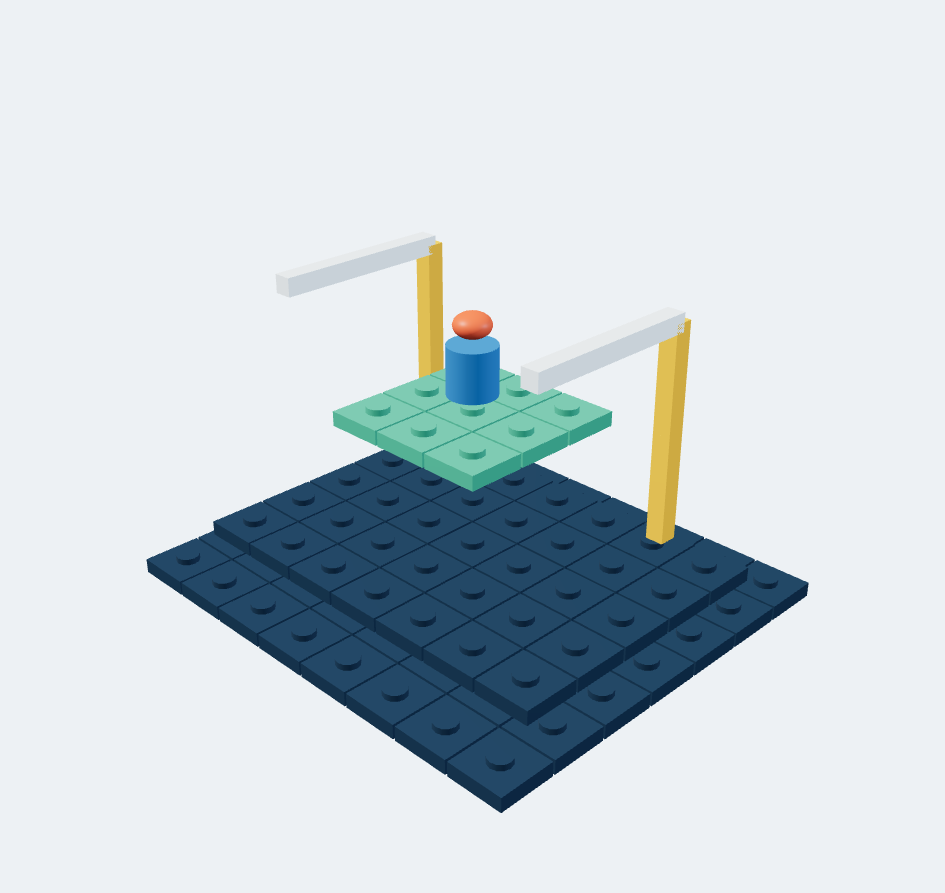
\includegraphics[width=.24\textwidth]{figures/hierarchy-expanded/exp-d1-suspension-2-iso.png}
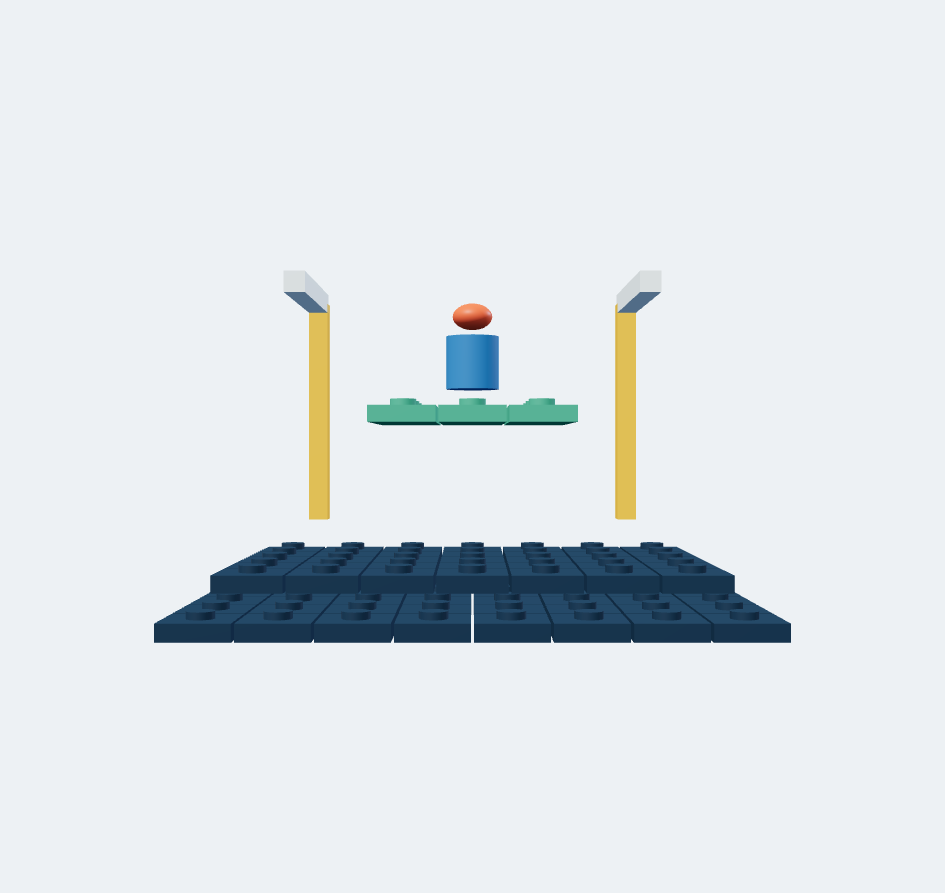
\includegraphics[width=.24\textwidth]{figures/hierarchy-expanded/exp-d1-suspension-2-front.png}
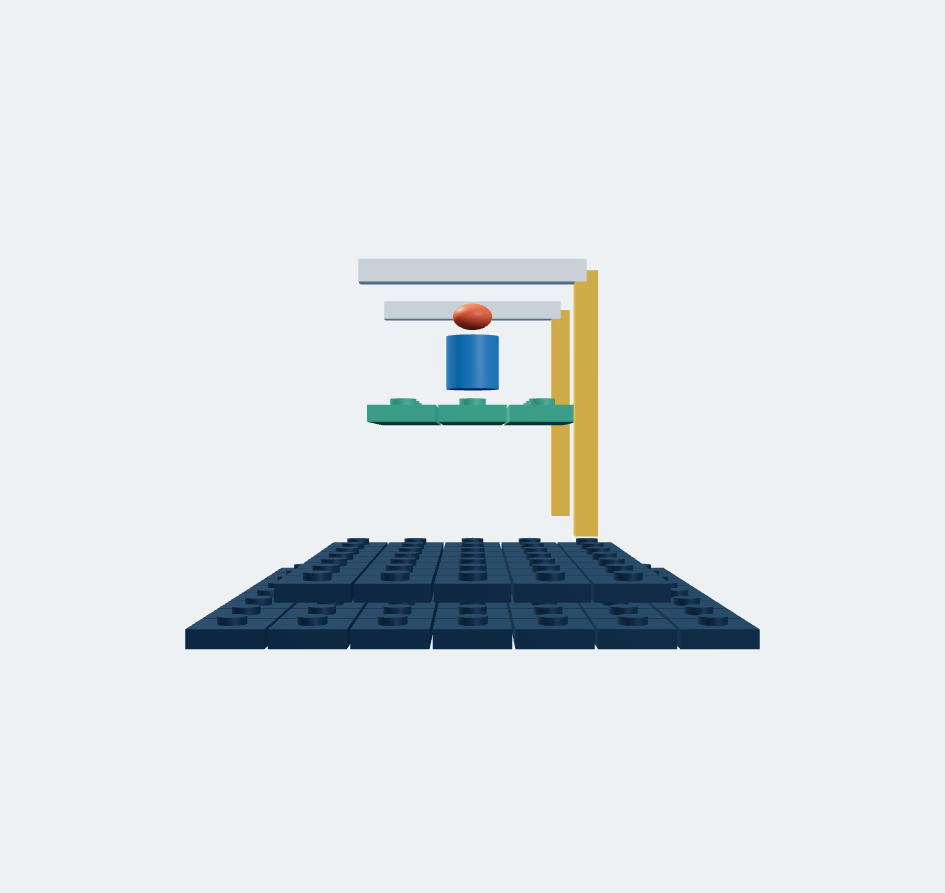
\includegraphics[width=.24\textwidth]{figures/hierarchy-expanded/exp-d1-suspension-2-side.png}
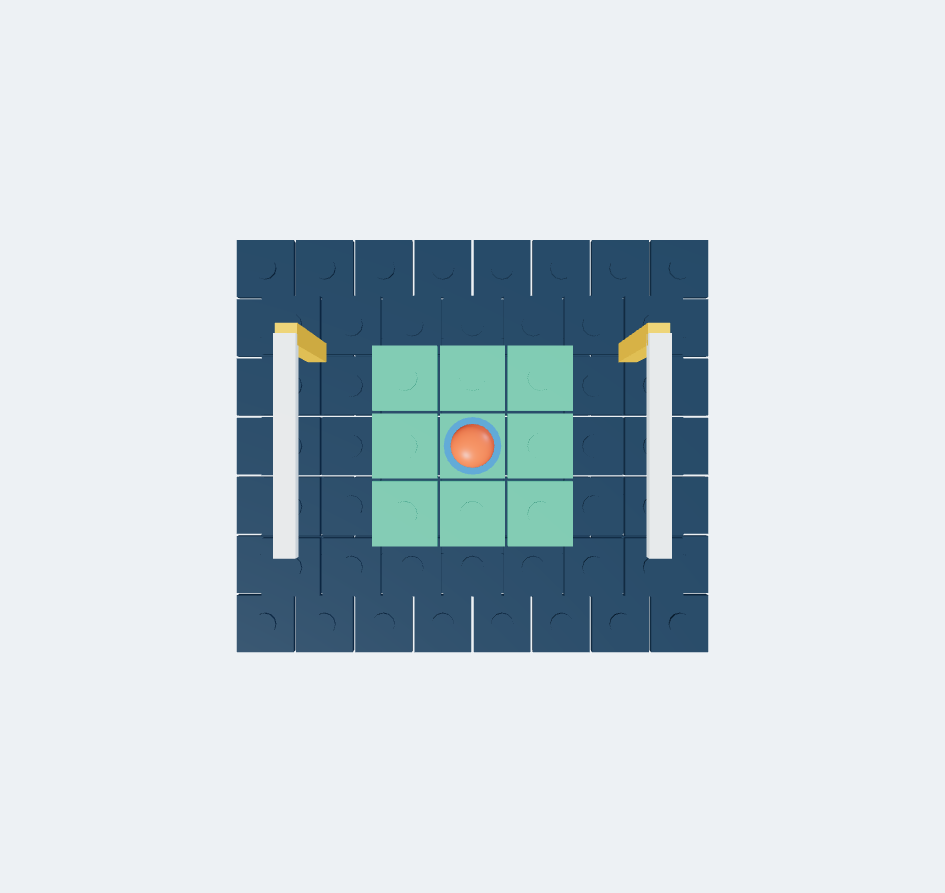
\includegraphics[width=.24\textwidth]{figures/hierarchy-expanded/exp-d1-suspension-2-top.png}
\end{center}
\noindent All 48 families share this source. Full inputs and answers appear in the companion question bank.
\begin{center}\tiny\begin{tabular}{rllll}\toprule No. & Family & Layer & Output & Evidence\\\midrule
1 & identify & atomic & single-choice & model-state \\
2 & count & atomic & single-choice & model-state \\
3 & color & atomic & single-choice & model-state \\
4 & position & atomic & single-choice & model-state \\
5 & joint-type & atomic & single-choice & model-state \\
6 & parent & atomic & single-choice & model-state \\
7 & anchor & atomic & single-choice & model-state \\
8 & degree & atomic & single-choice & model-state \\
9 & recolor & atomic & single-choice & model-state \\
10 & add & atomic & single-choice & model-state \\
11 & remove & atomic & single-choice & model-state \\
12 & replace & atomic & single-choice & model-state \\
13 & translate & atomic & single-choice & model-state \\
14 & rotate & atomic & single-choice & model-state \\
15 & next-module & atomic & single-choice & model-state \\
16 & inventory & atomic & single-choice & model-state \\
17 & boundary & atomic & single-choice & model-state \\
18 & no-op & atomic & single-choice & model-state \\
19 & prefix & metacognitive & single-choice & support-graph \\
20 & access & metacognitive & multiple-choice & Rapier \\
21 & counterfactual & metacognitive & single-choice & support-graph \\
22 & dynamic & metacognitive & single-choice & Rapier \\
23 & kinematic & metacognitive & multiple-choice & model-state \\
24 & diagnosis & metacognitive & multiple-choice & model-state \\
25 & information-gain & metacognitive & multiple-choice & finite-world \\
26 & abstention & metacognitive & single-choice & finite-world \\
27 & posterior & metacognitive & single-choice & finite-world \\
28 & pareto & metacognitive & multiple-choice & model-state \\
29 & assembly & procedural & actions & state-machine \\
30 & disassembly & procedural & actions & state-machine \\
31 & service-repair & procedural & actions & state-machine \\
32 & compound-edit & procedural & actions & state-machine \\
33 & multi-fault & integrative & actions & state-machine \\
34 & scheduling & integrative & schedule & resource-schedule \\
35 & policy & integrative & policy & finite-world \\
36 & local-frame & atomic & single-choice & model-state \\
37 & projection & atomic & single-choice & model-state \\
38 & relative-order & atomic & single-choice & model-state \\
39 & joint-axis & atomic & single-choice & model-state \\
40 & clearance-margin & metacognitive & single-choice & model-state \\
41 & load-moment & metacognitive & single-choice & model-state \\
42 & weighted-posterior & metacognitive & single-choice & finite-world \\
43 & expected-loss & metacognitive & single-choice & finite-world \\
44 & trace-threshold & metacognitive & single-choice & Rapier \\
45 & guarded-repair & procedural & actions & state-machine \\
46 & rollback & procedural & actions & state-machine \\
47 & resource-repair & integrative & actions & state-machine \\
48 & budget-policy & integrative & policy & finite-world \\
\bottomrule\end{tabular}\end{center}
\clearpage
\subsection{22. Offset-load Turntable (D1)}
105 visible parts; 5 modules; 4 joints. Representative-point motion 0.0000; rotation 0.0000 rad.
\begin{center}
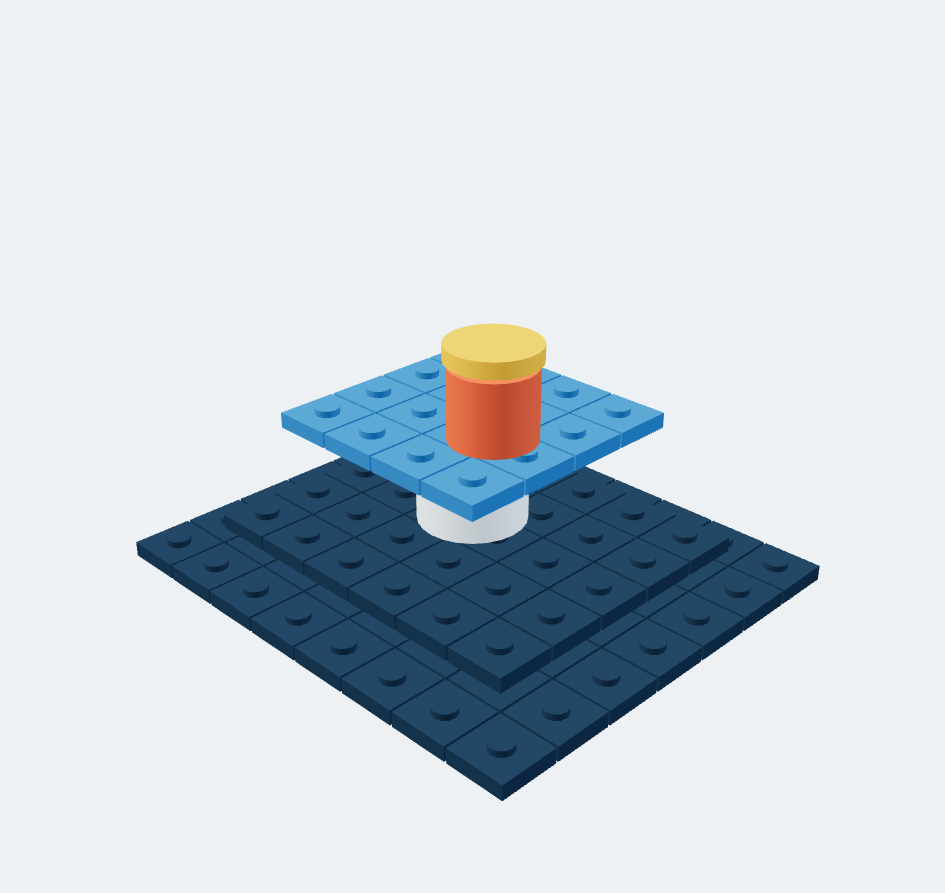
\includegraphics[width=.24\textwidth]{figures/hierarchy-expanded/exp-d1-turntable-1-iso.png}
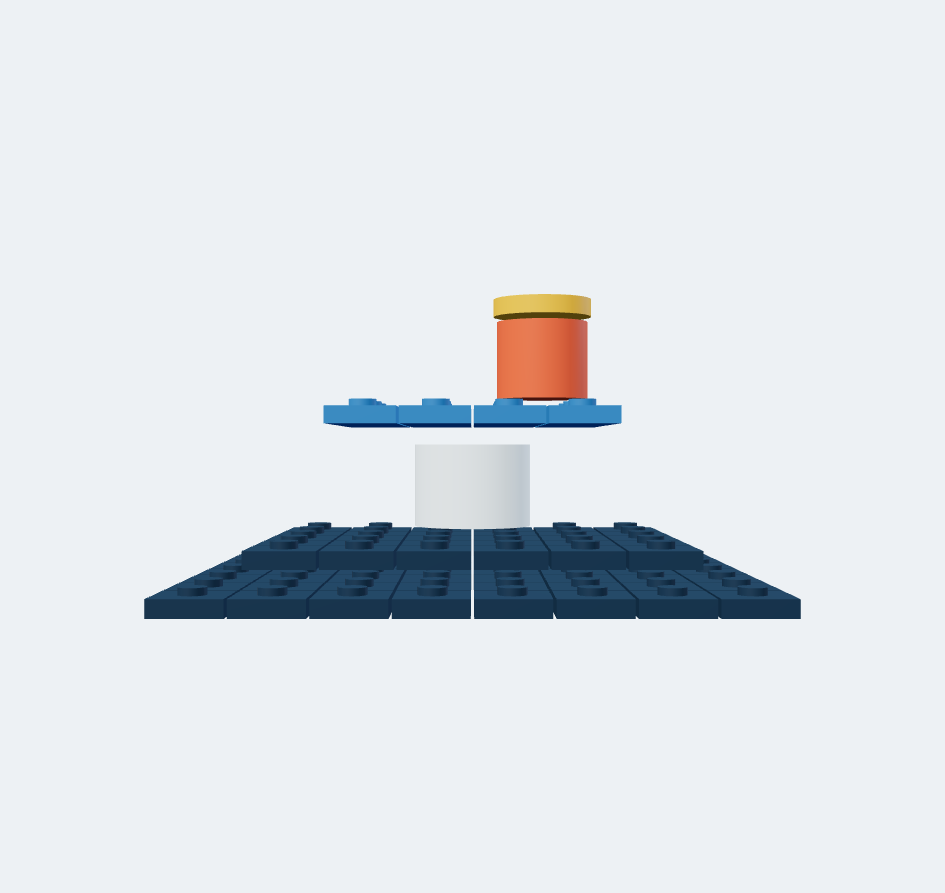
\includegraphics[width=.24\textwidth]{figures/hierarchy-expanded/exp-d1-turntable-1-front.png}
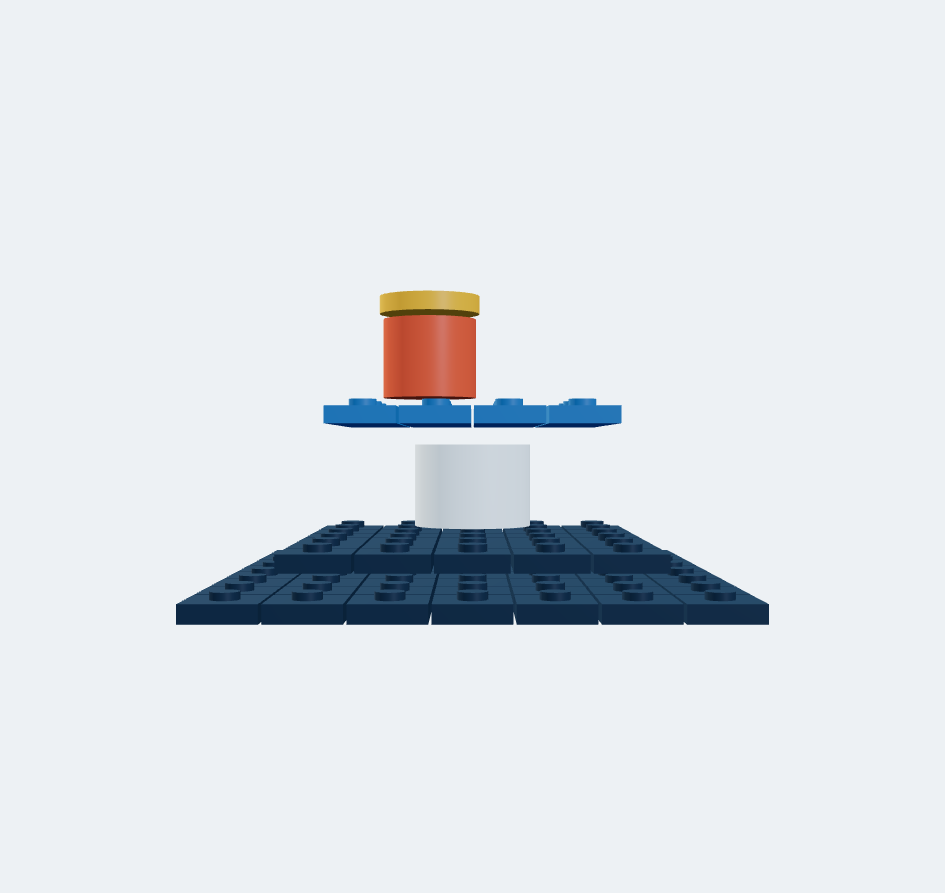
\includegraphics[width=.24\textwidth]{figures/hierarchy-expanded/exp-d1-turntable-1-side.png}
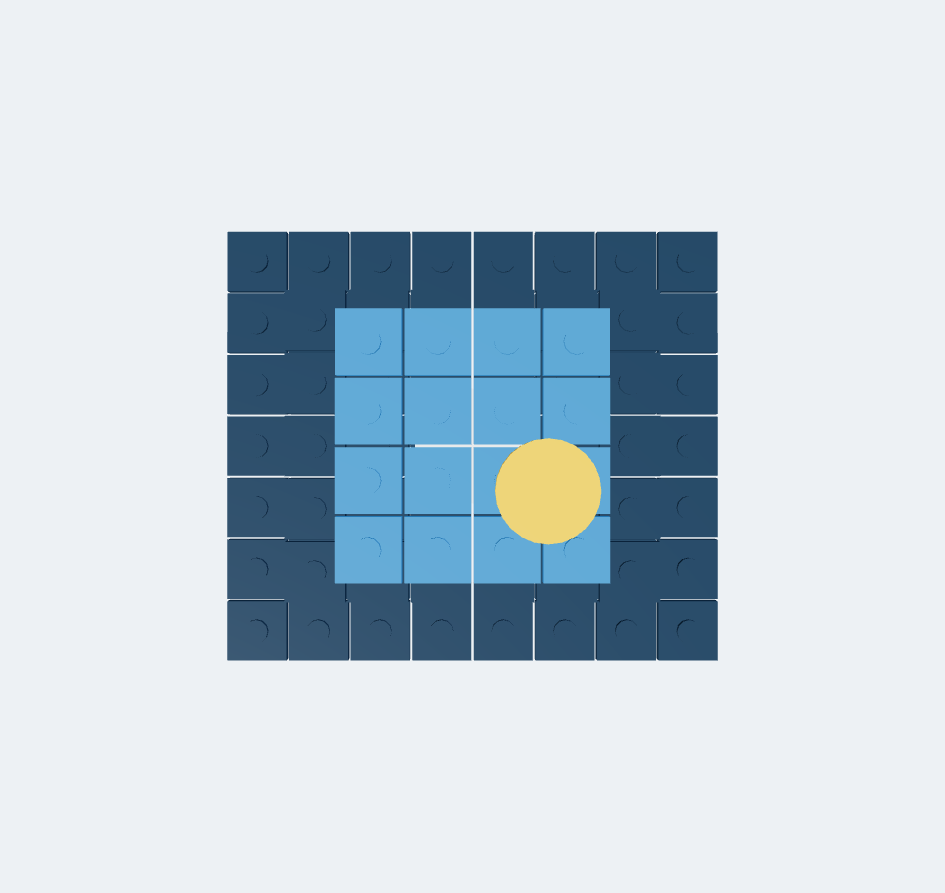
\includegraphics[width=.24\textwidth]{figures/hierarchy-expanded/exp-d1-turntable-1-top.png}
\end{center}
\noindent All 48 families share this source. Full inputs and answers appear in the companion question bank.
\begin{center}\tiny\begin{tabular}{rllll}\toprule No. & Family & Layer & Output & Evidence\\\midrule
1 & identify & atomic & single-choice & model-state \\
2 & count & atomic & single-choice & model-state \\
3 & color & atomic & single-choice & model-state \\
4 & position & atomic & single-choice & model-state \\
5 & joint-type & atomic & single-choice & model-state \\
6 & parent & atomic & single-choice & model-state \\
7 & anchor & atomic & single-choice & model-state \\
8 & degree & atomic & single-choice & model-state \\
9 & recolor & atomic & single-choice & model-state \\
10 & add & atomic & single-choice & model-state \\
11 & remove & atomic & single-choice & model-state \\
12 & replace & atomic & single-choice & model-state \\
13 & translate & atomic & single-choice & model-state \\
14 & rotate & atomic & single-choice & model-state \\
15 & next-module & atomic & single-choice & model-state \\
16 & inventory & atomic & single-choice & model-state \\
17 & boundary & atomic & single-choice & model-state \\
18 & no-op & atomic & single-choice & model-state \\
19 & prefix & metacognitive & single-choice & support-graph \\
20 & access & metacognitive & multiple-choice & Rapier \\
21 & counterfactual & metacognitive & single-choice & support-graph \\
22 & dynamic & metacognitive & single-choice & Rapier \\
23 & kinematic & metacognitive & multiple-choice & model-state \\
24 & diagnosis & metacognitive & multiple-choice & model-state \\
25 & information-gain & metacognitive & multiple-choice & finite-world \\
26 & abstention & metacognitive & single-choice & finite-world \\
27 & posterior & metacognitive & single-choice & finite-world \\
28 & pareto & metacognitive & multiple-choice & model-state \\
29 & assembly & procedural & actions & state-machine \\
30 & disassembly & procedural & actions & state-machine \\
31 & service-repair & procedural & actions & state-machine \\
32 & compound-edit & procedural & actions & state-machine \\
33 & multi-fault & integrative & actions & state-machine \\
34 & scheduling & integrative & schedule & resource-schedule \\
35 & policy & integrative & policy & finite-world \\
36 & local-frame & atomic & single-choice & model-state \\
37 & projection & atomic & single-choice & model-state \\
38 & relative-order & atomic & single-choice & model-state \\
39 & joint-axis & atomic & single-choice & model-state \\
40 & clearance-margin & metacognitive & single-choice & model-state \\
41 & load-moment & metacognitive & single-choice & model-state \\
42 & weighted-posterior & metacognitive & single-choice & finite-world \\
43 & expected-loss & metacognitive & single-choice & finite-world \\
44 & trace-threshold & metacognitive & single-choice & Rapier \\
45 & guarded-repair & procedural & actions & state-machine \\
46 & rollback & procedural & actions & state-machine \\
47 & resource-repair & integrative & actions & state-machine \\
48 & budget-policy & integrative & policy & finite-world \\
\bottomrule\end{tabular}\end{center}
\clearpage
\subsection{23. Two-tier Service Turntable (D1)}
114 visible parts; 6 modules; 5 joints. Representative-point motion 0.0001; rotation 0.0000 rad.
\begin{center}
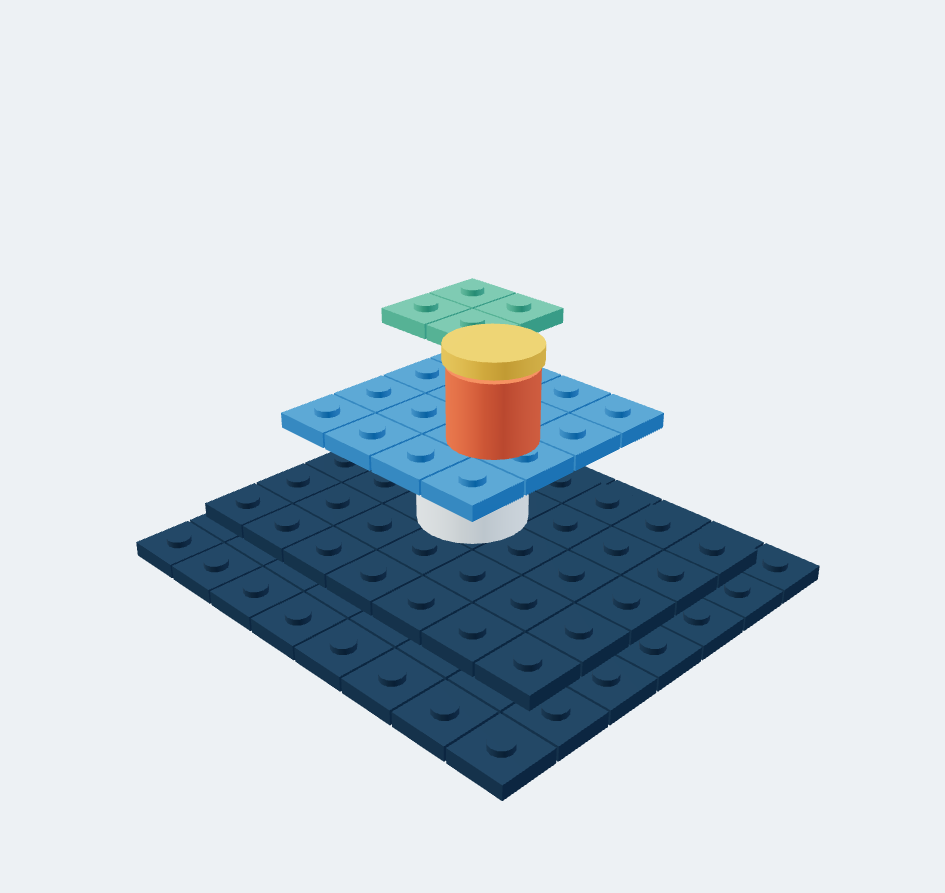
\includegraphics[width=.24\textwidth]{figures/hierarchy-expanded/exp-d1-turntable-2-iso.png}
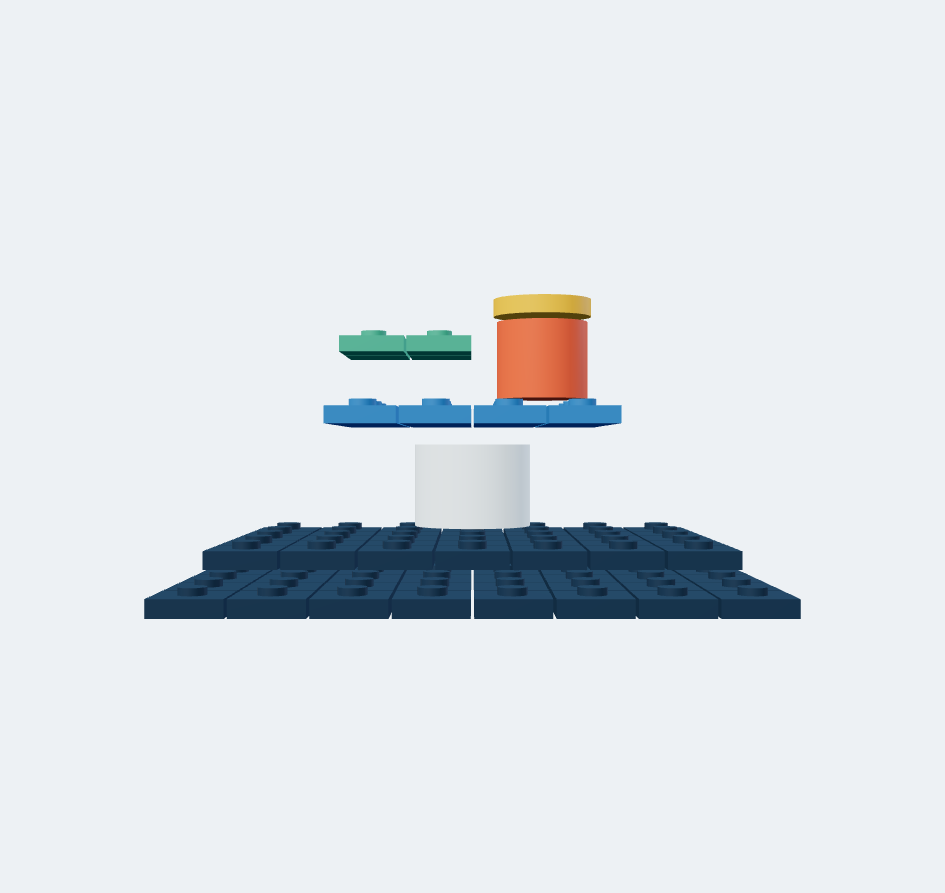
\includegraphics[width=.24\textwidth]{figures/hierarchy-expanded/exp-d1-turntable-2-front.png}
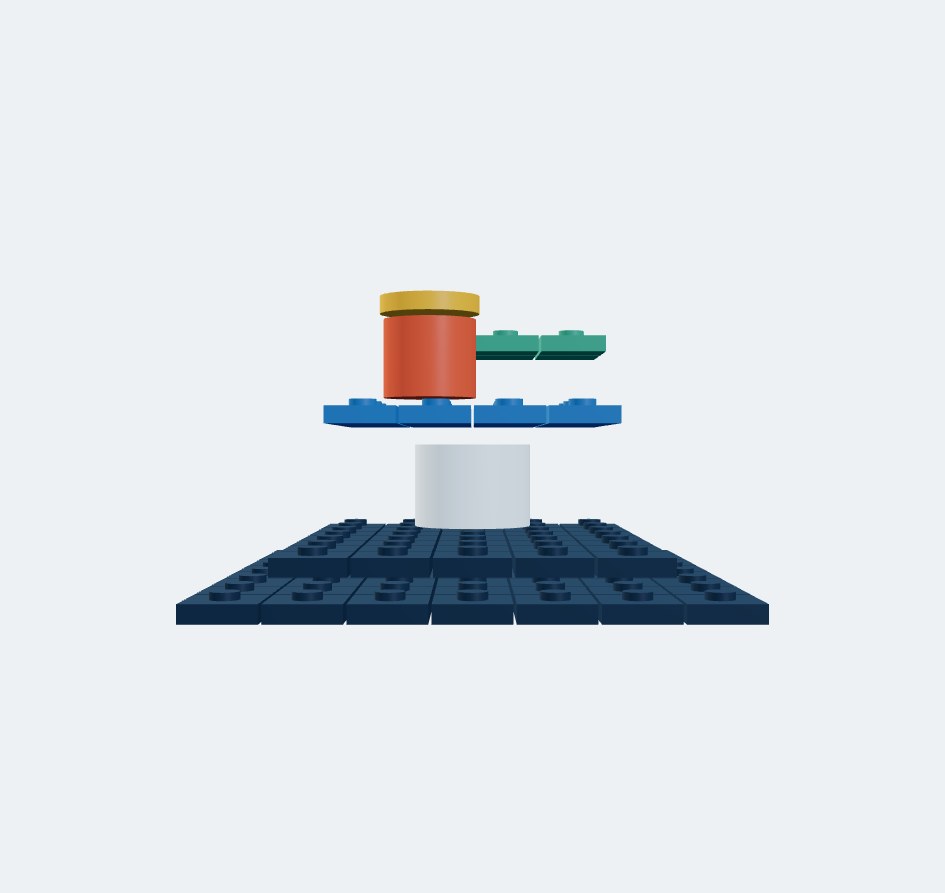
\includegraphics[width=.24\textwidth]{figures/hierarchy-expanded/exp-d1-turntable-2-side.png}
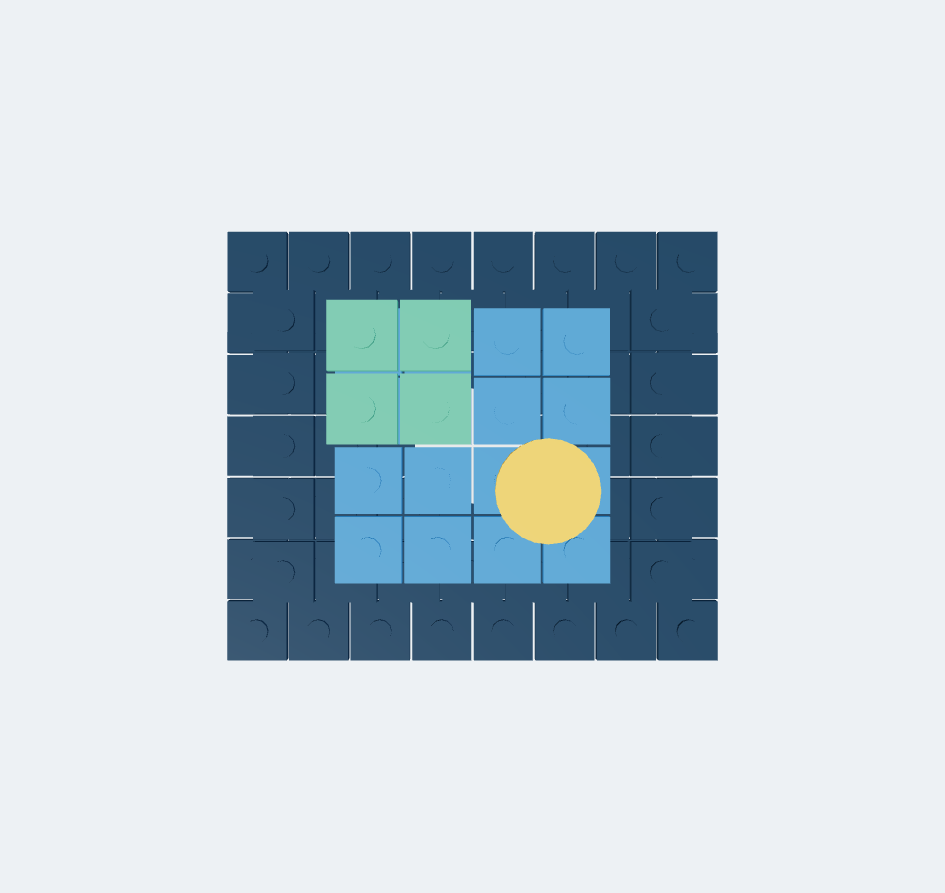
\includegraphics[width=.24\textwidth]{figures/hierarchy-expanded/exp-d1-turntable-2-top.png}
\end{center}
\noindent All 48 families share this source. Full inputs and answers appear in the companion question bank.
\begin{center}\tiny\begin{tabular}{rllll}\toprule No. & Family & Layer & Output & Evidence\\\midrule
1 & identify & atomic & single-choice & model-state \\
2 & count & atomic & single-choice & model-state \\
3 & color & atomic & single-choice & model-state \\
4 & position & atomic & single-choice & model-state \\
5 & joint-type & atomic & single-choice & model-state \\
6 & parent & atomic & single-choice & model-state \\
7 & anchor & atomic & single-choice & model-state \\
8 & degree & atomic & single-choice & model-state \\
9 & recolor & atomic & single-choice & model-state \\
10 & add & atomic & single-choice & model-state \\
11 & remove & atomic & single-choice & model-state \\
12 & replace & atomic & single-choice & model-state \\
13 & translate & atomic & single-choice & model-state \\
14 & rotate & atomic & single-choice & model-state \\
15 & next-module & atomic & single-choice & model-state \\
16 & inventory & atomic & single-choice & model-state \\
17 & boundary & atomic & single-choice & model-state \\
18 & no-op & atomic & single-choice & model-state \\
19 & prefix & metacognitive & single-choice & support-graph \\
20 & access & metacognitive & multiple-choice & Rapier \\
21 & counterfactual & metacognitive & single-choice & support-graph \\
22 & dynamic & metacognitive & single-choice & Rapier \\
23 & kinematic & metacognitive & multiple-choice & model-state \\
24 & diagnosis & metacognitive & multiple-choice & model-state \\
25 & information-gain & metacognitive & multiple-choice & finite-world \\
26 & abstention & metacognitive & single-choice & finite-world \\
27 & posterior & metacognitive & single-choice & finite-world \\
28 & pareto & metacognitive & multiple-choice & model-state \\
29 & assembly & procedural & actions & state-machine \\
30 & disassembly & procedural & actions & state-machine \\
31 & service-repair & procedural & actions & state-machine \\
32 & compound-edit & procedural & actions & state-machine \\
33 & multi-fault & integrative & actions & state-machine \\
34 & scheduling & integrative & schedule & resource-schedule \\
35 & policy & integrative & policy & finite-world \\
36 & local-frame & atomic & single-choice & model-state \\
37 & projection & atomic & single-choice & model-state \\
38 & relative-order & atomic & single-choice & model-state \\
39 & joint-axis & atomic & single-choice & model-state \\
40 & clearance-margin & metacognitive & single-choice & model-state \\
41 & load-moment & metacognitive & single-choice & model-state \\
42 & weighted-posterior & metacognitive & single-choice & finite-world \\
43 & expected-loss & metacognitive & single-choice & finite-world \\
44 & trace-threshold & metacognitive & single-choice & Rapier \\
45 & guarded-repair & procedural & actions & state-machine \\
46 & rollback & procedural & actions & state-machine \\
47 & resource-repair & integrative & actions & state-machine \\
48 & budget-policy & integrative & policy & finite-world \\
\bottomrule\end{tabular}\end{center}
\clearpage
\subsection{24. Folding Twin Wings (D1)}
99 visible parts; 5 modules; 4 joints. Representative-point motion 0.0000; rotation 0.0000 rad.
\begin{center}
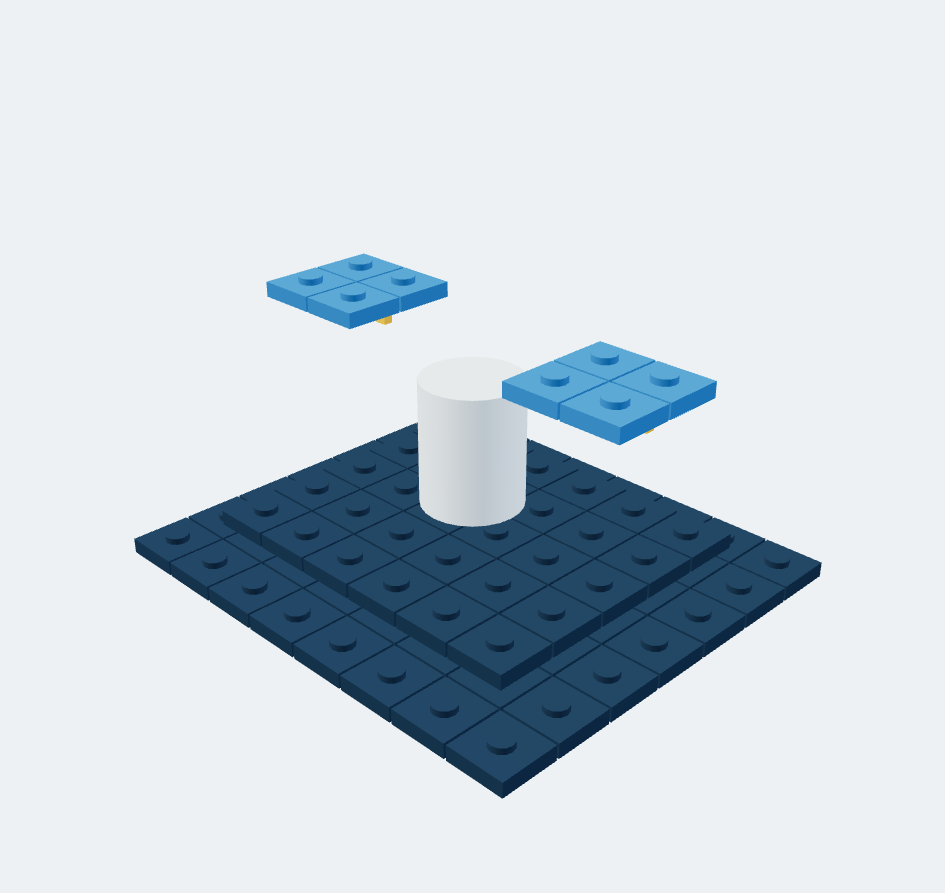
\includegraphics[width=.24\textwidth]{figures/hierarchy-expanded/exp-d1-wings-1-iso.png}
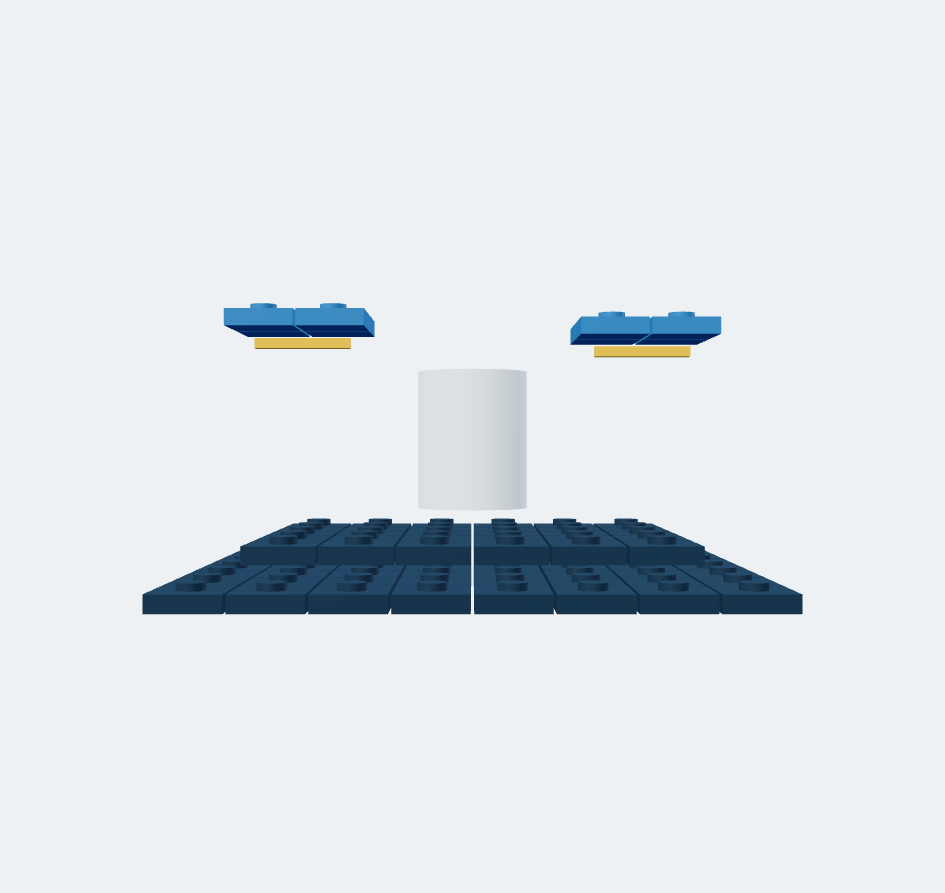
\includegraphics[width=.24\textwidth]{figures/hierarchy-expanded/exp-d1-wings-1-front.png}

\includegraphics[width=.24\textwidth]{figures/hierarchy-expanded/exp-d1-wings-1-side.png}
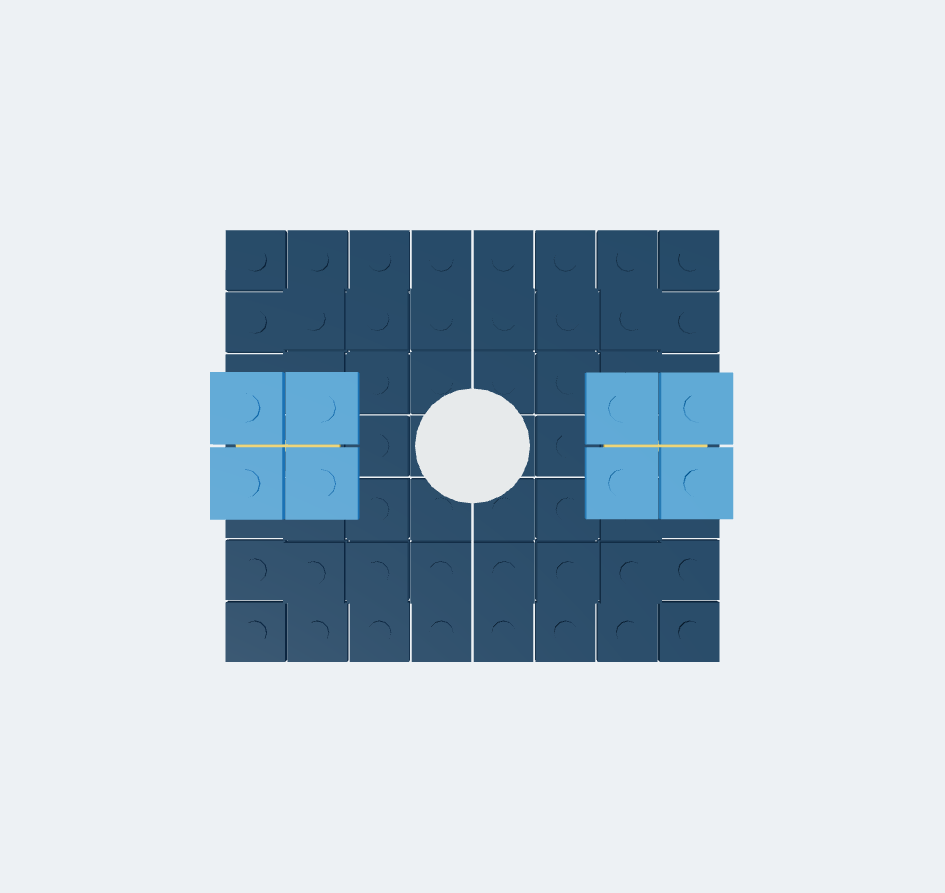
\includegraphics[width=.24\textwidth]{figures/hierarchy-expanded/exp-d1-wings-1-top.png}
\end{center}
\noindent All 48 families share this source. Full inputs and answers appear in the companion question bank.
\begin{center}\tiny\begin{tabular}{rllll}\toprule No. & Family & Layer & Output & Evidence\\\midrule
1 & identify & atomic & single-choice & model-state \\
2 & count & atomic & single-choice & model-state \\
3 & color & atomic & single-choice & model-state \\
4 & position & atomic & single-choice & model-state \\
5 & joint-type & atomic & single-choice & model-state \\
6 & parent & atomic & single-choice & model-state \\
7 & anchor & atomic & single-choice & model-state \\
8 & degree & atomic & single-choice & model-state \\
9 & recolor & atomic & single-choice & model-state \\
10 & add & atomic & single-choice & model-state \\
11 & remove & atomic & single-choice & model-state \\
12 & replace & atomic & single-choice & model-state \\
13 & translate & atomic & single-choice & model-state \\
14 & rotate & atomic & single-choice & model-state \\
15 & next-module & atomic & single-choice & model-state \\
16 & inventory & atomic & single-choice & model-state \\
17 & boundary & atomic & single-choice & model-state \\
18 & no-op & atomic & single-choice & model-state \\
19 & prefix & metacognitive & single-choice & support-graph \\
20 & access & metacognitive & multiple-choice & Rapier \\
21 & counterfactual & metacognitive & single-choice & support-graph \\
22 & dynamic & metacognitive & single-choice & Rapier \\
23 & kinematic & metacognitive & multiple-choice & model-state \\
24 & diagnosis & metacognitive & multiple-choice & model-state \\
25 & information-gain & metacognitive & multiple-choice & finite-world \\
26 & abstention & metacognitive & single-choice & finite-world \\
27 & posterior & metacognitive & single-choice & finite-world \\
28 & pareto & metacognitive & multiple-choice & model-state \\
29 & assembly & procedural & actions & state-machine \\
30 & disassembly & procedural & actions & state-machine \\
31 & service-repair & procedural & actions & state-machine \\
32 & compound-edit & procedural & actions & state-machine \\
33 & multi-fault & integrative & actions & state-machine \\
34 & scheduling & integrative & schedule & resource-schedule \\
35 & policy & integrative & policy & finite-world \\
36 & local-frame & atomic & single-choice & model-state \\
37 & projection & atomic & single-choice & model-state \\
38 & relative-order & atomic & single-choice & model-state \\
39 & joint-axis & atomic & single-choice & model-state \\
40 & clearance-margin & metacognitive & single-choice & model-state \\
41 & load-moment & metacognitive & single-choice & model-state \\
42 & weighted-posterior & metacognitive & single-choice & finite-world \\
43 & expected-loss & metacognitive & single-choice & finite-world \\
44 & trace-threshold & metacognitive & single-choice & Rapier \\
45 & guarded-repair & procedural & actions & state-machine \\
46 & rollback & procedural & actions & state-machine \\
47 & resource-repair & integrative & actions & state-machine \\
48 & budget-policy & integrative & policy & finite-world \\
\bottomrule\end{tabular}\end{center}
\clearpage
\subsection{25. Four-petal Panel Array (D1)}
124 visible parts; 7 modules; 6 joints. Representative-point motion 0.0000; rotation 0.0000 rad.
\begin{center}
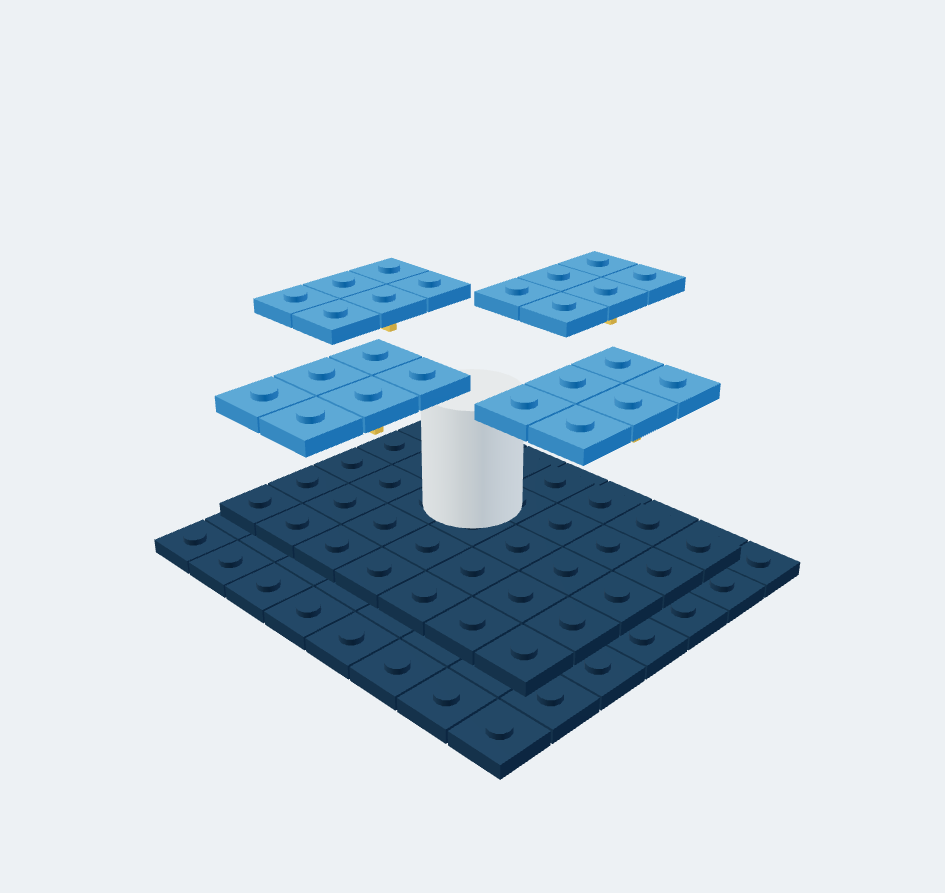
\includegraphics[width=.24\textwidth]{figures/hierarchy-expanded/exp-d1-wings-2-iso.png}
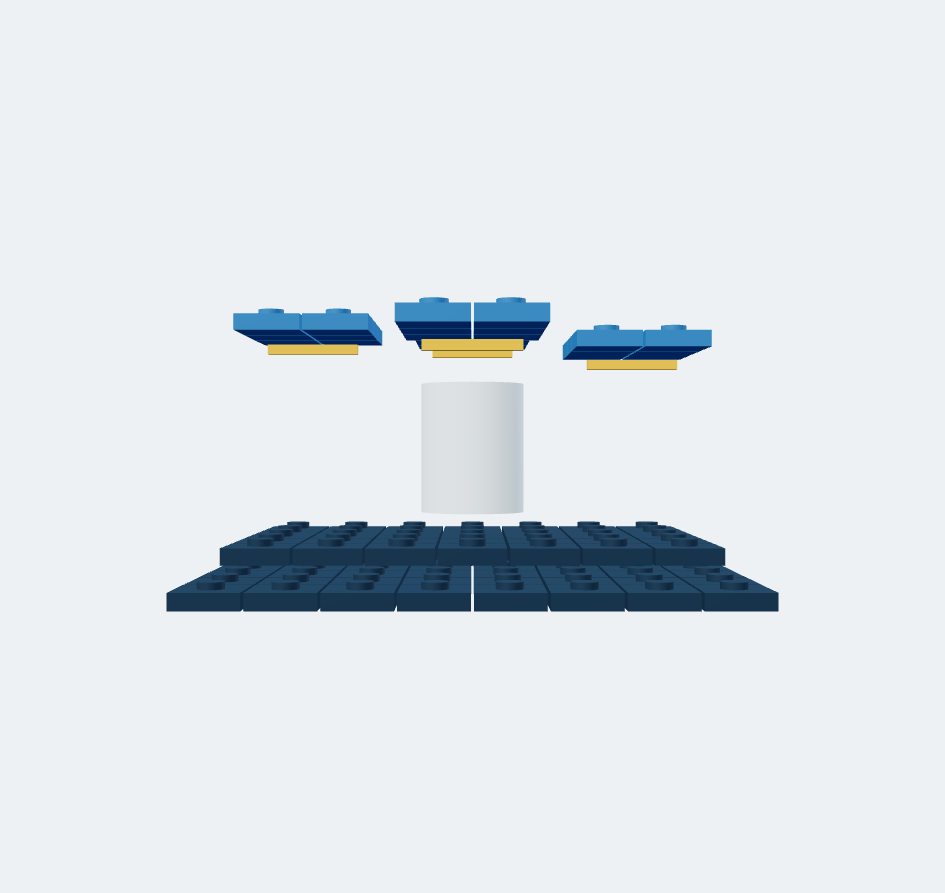
\includegraphics[width=.24\textwidth]{figures/hierarchy-expanded/exp-d1-wings-2-front.png}
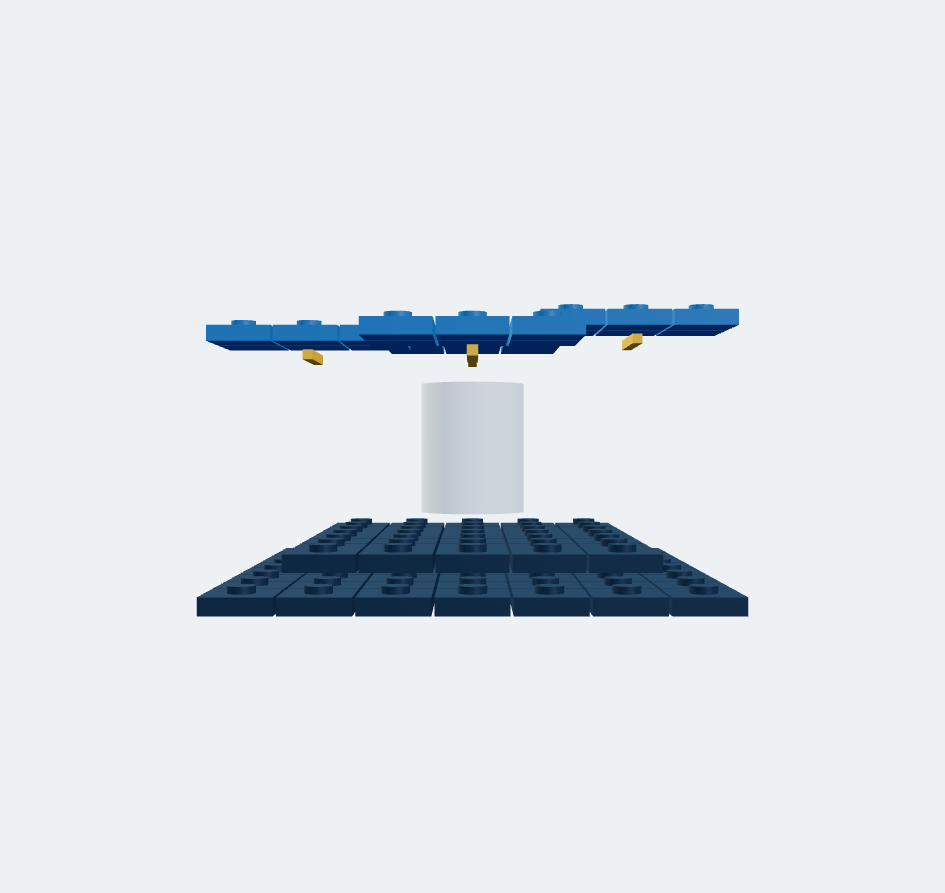
\includegraphics[width=.24\textwidth]{figures/hierarchy-expanded/exp-d1-wings-2-side.png}
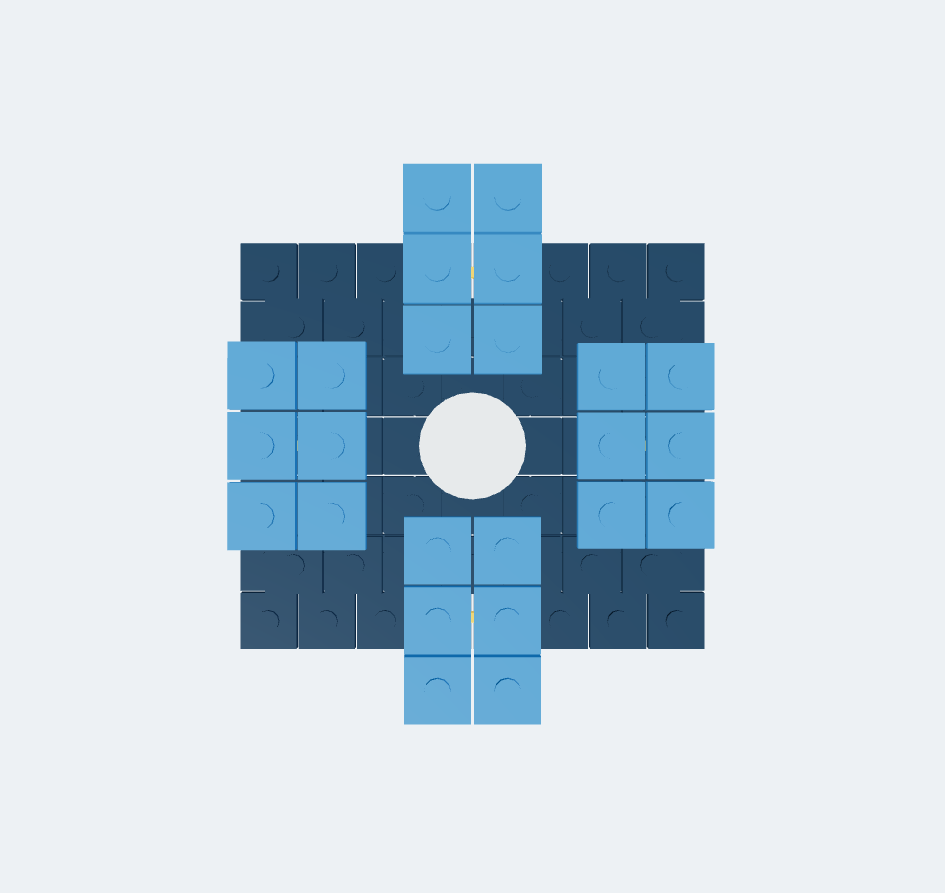
\includegraphics[width=.24\textwidth]{figures/hierarchy-expanded/exp-d1-wings-2-top.png}
\end{center}
\noindent All 48 families share this source. Full inputs and answers appear in the companion question bank.
\begin{center}\tiny\begin{tabular}{rllll}\toprule No. & Family & Layer & Output & Evidence\\\midrule
1 & identify & atomic & single-choice & model-state \\
2 & count & atomic & single-choice & model-state \\
3 & color & atomic & single-choice & model-state \\
4 & position & atomic & single-choice & model-state \\
5 & joint-type & atomic & single-choice & model-state \\
6 & parent & atomic & single-choice & model-state \\
7 & anchor & atomic & single-choice & model-state \\
8 & degree & atomic & single-choice & model-state \\
9 & recolor & atomic & single-choice & model-state \\
10 & add & atomic & single-choice & model-state \\
11 & remove & atomic & single-choice & model-state \\
12 & replace & atomic & single-choice & model-state \\
13 & translate & atomic & single-choice & model-state \\
14 & rotate & atomic & single-choice & model-state \\
15 & next-module & atomic & single-choice & model-state \\
16 & inventory & atomic & single-choice & model-state \\
17 & boundary & atomic & single-choice & model-state \\
18 & no-op & atomic & single-choice & model-state \\
19 & prefix & metacognitive & single-choice & support-graph \\
20 & access & metacognitive & multiple-choice & Rapier \\
21 & counterfactual & metacognitive & single-choice & support-graph \\
22 & dynamic & metacognitive & single-choice & Rapier \\
23 & kinematic & metacognitive & multiple-choice & model-state \\
24 & diagnosis & metacognitive & multiple-choice & model-state \\
25 & information-gain & metacognitive & multiple-choice & finite-world \\
26 & abstention & metacognitive & single-choice & finite-world \\
27 & posterior & metacognitive & single-choice & finite-world \\
28 & pareto & metacognitive & multiple-choice & model-state \\
29 & assembly & procedural & actions & state-machine \\
30 & disassembly & procedural & actions & state-machine \\
31 & service-repair & procedural & actions & state-machine \\
32 & compound-edit & procedural & actions & state-machine \\
33 & multi-fault & integrative & actions & state-machine \\
34 & scheduling & integrative & schedule & resource-schedule \\
35 & policy & integrative & policy & finite-world \\
36 & local-frame & atomic & single-choice & model-state \\
37 & projection & atomic & single-choice & model-state \\
38 & relative-order & atomic & single-choice & model-state \\
39 & joint-axis & atomic & single-choice & model-state \\
40 & clearance-margin & metacognitive & single-choice & model-state \\
41 & load-moment & metacognitive & single-choice & model-state \\
42 & weighted-posterior & metacognitive & single-choice & finite-world \\
43 & expected-loss & metacognitive & single-choice & finite-world \\
44 & trace-threshold & metacognitive & single-choice & Rapier \\
45 & guarded-repair & procedural & actions & state-machine \\
46 & rollback & procedural & actions & state-machine \\
47 & resource-repair & integrative & actions & state-machine \\
48 & budget-policy & integrative & policy & finite-world \\
\bottomrule\end{tabular}\end{center}
\clearpage
\subsection{26. Folding Gripper (D1)}
19 visible parts; 5 modules; 4 joints. Representative-point motion 0.0005; rotation 0.0000 rad.
\begin{center}

\includegraphics[width=.24\textwidth]{figures/hierarchy-expanded/folding-gripper-iso.png}

\includegraphics[width=.24\textwidth]{figures/hierarchy-expanded/folding-gripper-front.png}

\includegraphics[width=.24\textwidth]{figures/hierarchy-expanded/folding-gripper-side.png}

\includegraphics[width=.24\textwidth]{figures/hierarchy-expanded/folding-gripper-top.png}
\end{center}
\noindent All 48 families share this source. Full inputs and answers appear in the companion question bank.
\begin{center}\tiny\begin{tabular}{rllll}\toprule No. & Family & Layer & Output & Evidence\\\midrule
1 & identify & atomic & single-choice & model-state \\
2 & count & atomic & single-choice & model-state \\
3 & color & atomic & single-choice & model-state \\
4 & position & atomic & single-choice & model-state \\
5 & joint-type & atomic & single-choice & model-state \\
6 & parent & atomic & single-choice & model-state \\
7 & anchor & atomic & single-choice & model-state \\
8 & degree & atomic & single-choice & model-state \\
9 & recolor & atomic & single-choice & model-state \\
10 & add & atomic & single-choice & model-state \\
11 & remove & atomic & single-choice & model-state \\
12 & replace & atomic & single-choice & model-state \\
13 & translate & atomic & single-choice & model-state \\
14 & rotate & atomic & single-choice & model-state \\
15 & next-module & atomic & single-choice & model-state \\
16 & inventory & atomic & single-choice & model-state \\
17 & boundary & atomic & single-choice & model-state \\
18 & no-op & atomic & single-choice & model-state \\
19 & prefix & metacognitive & single-choice & support-graph \\
20 & access & metacognitive & multiple-choice & Rapier \\
21 & counterfactual & metacognitive & single-choice & support-graph \\
22 & dynamic & metacognitive & single-choice & Rapier \\
23 & kinematic & metacognitive & multiple-choice & model-state \\
24 & diagnosis & metacognitive & multiple-choice & model-state \\
25 & information-gain & metacognitive & multiple-choice & finite-world \\
26 & abstention & metacognitive & single-choice & finite-world \\
27 & posterior & metacognitive & single-choice & finite-world \\
28 & pareto & metacognitive & multiple-choice & model-state \\
29 & assembly & procedural & actions & state-machine \\
30 & disassembly & procedural & actions & state-machine \\
31 & service-repair & procedural & actions & state-machine \\
32 & compound-edit & procedural & actions & state-machine \\
33 & multi-fault & integrative & actions & state-machine \\
34 & scheduling & integrative & schedule & resource-schedule \\
35 & policy & integrative & policy & finite-world \\
36 & local-frame & atomic & single-choice & model-state \\
37 & projection & atomic & single-choice & model-state \\
38 & relative-order & atomic & single-choice & model-state \\
39 & joint-axis & atomic & single-choice & model-state \\
40 & clearance-margin & metacognitive & single-choice & model-state \\
41 & load-moment & metacognitive & single-choice & model-state \\
42 & weighted-posterior & metacognitive & single-choice & finite-world \\
43 & expected-loss & metacognitive & single-choice & finite-world \\
44 & trace-threshold & metacognitive & single-choice & Rapier \\
45 & guarded-repair & procedural & actions & state-machine \\
46 & rollback & procedural & actions & state-machine \\
47 & resource-repair & integrative & actions & state-machine \\
48 & budget-policy & integrative & policy & finite-world \\
\bottomrule\end{tabular}\end{center}
\clearpage
\subsection{27. Hinged Safety Hatch (D1)}
28 visible parts; 3 modules; 2 joints. Representative-point motion 0.0000; rotation 0.0000 rad.
\begin{center}

\includegraphics[width=.24\textwidth]{figures/hierarchy-expanded/hinged-safety-hatch-iso.png}

\includegraphics[width=.24\textwidth]{figures/hierarchy-expanded/hinged-safety-hatch-front.png}

\includegraphics[width=.24\textwidth]{figures/hierarchy-expanded/hinged-safety-hatch-side.png}

\includegraphics[width=.24\textwidth]{figures/hierarchy-expanded/hinged-safety-hatch-top.png}
\end{center}
\noindent All 48 families share this source. Full inputs and answers appear in the companion question bank.
\begin{center}\tiny\begin{tabular}{rllll}\toprule No. & Family & Layer & Output & Evidence\\\midrule
1 & identify & atomic & single-choice & model-state \\
2 & count & atomic & single-choice & model-state \\
3 & color & atomic & single-choice & model-state \\
4 & position & atomic & single-choice & model-state \\
5 & joint-type & atomic & single-choice & model-state \\
6 & parent & atomic & single-choice & model-state \\
7 & anchor & atomic & single-choice & model-state \\
8 & degree & atomic & single-choice & model-state \\
9 & recolor & atomic & single-choice & model-state \\
10 & add & atomic & single-choice & model-state \\
11 & remove & atomic & single-choice & model-state \\
12 & replace & atomic & single-choice & model-state \\
13 & translate & atomic & single-choice & model-state \\
14 & rotate & atomic & single-choice & model-state \\
15 & next-module & atomic & single-choice & model-state \\
16 & inventory & atomic & single-choice & model-state \\
17 & boundary & atomic & single-choice & model-state \\
18 & no-op & atomic & single-choice & model-state \\
19 & prefix & metacognitive & single-choice & support-graph \\
20 & access & metacognitive & multiple-choice & Rapier \\
21 & counterfactual & metacognitive & single-choice & support-graph \\
22 & dynamic & metacognitive & single-choice & Rapier \\
23 & kinematic & metacognitive & multiple-choice & model-state \\
24 & diagnosis & metacognitive & multiple-choice & model-state \\
25 & information-gain & metacognitive & multiple-choice & finite-world \\
26 & abstention & metacognitive & single-choice & finite-world \\
27 & posterior & metacognitive & single-choice & finite-world \\
28 & pareto & metacognitive & multiple-choice & model-state \\
29 & assembly & procedural & actions & state-machine \\
30 & disassembly & procedural & actions & state-machine \\
31 & service-repair & procedural & actions & state-machine \\
32 & compound-edit & procedural & actions & state-machine \\
33 & multi-fault & integrative & actions & state-machine \\
34 & scheduling & integrative & schedule & resource-schedule \\
35 & policy & integrative & policy & finite-world \\
36 & local-frame & atomic & single-choice & model-state \\
37 & projection & atomic & single-choice & model-state \\
38 & relative-order & atomic & single-choice & model-state \\
39 & joint-axis & atomic & single-choice & model-state \\
40 & clearance-margin & metacognitive & single-choice & model-state \\
41 & load-moment & metacognitive & single-choice & model-state \\
42 & weighted-posterior & metacognitive & single-choice & finite-world \\
43 & expected-loss & metacognitive & single-choice & finite-world \\
44 & trace-threshold & metacognitive & single-choice & Rapier \\
45 & guarded-repair & procedural & actions & state-machine \\
46 & rollback & procedural & actions & state-machine \\
47 & resource-repair & integrative & actions & state-machine \\
48 & budget-policy & integrative & policy & finite-world \\
\bottomrule\end{tabular}\end{center}
\clearpage
\subsection{28. Indexed Toggle Latch (D1)}
25 visible parts; 6 modules; 5 joints. Representative-point motion 0.0000; rotation 0.0000 rad.
\begin{center}

\includegraphics[width=.24\textwidth]{figures/hierarchy-expanded/indexed-toggle-latch-iso.png}
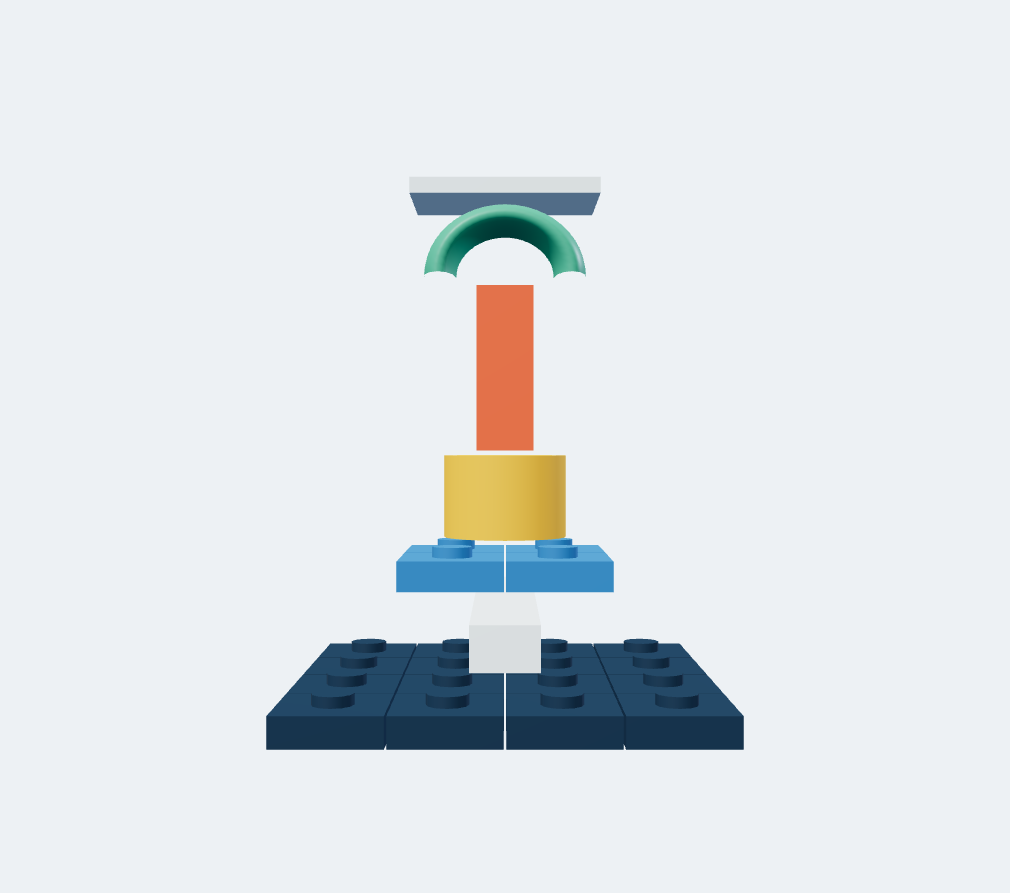
\includegraphics[width=.24\textwidth]{figures/hierarchy-expanded/indexed-toggle-latch-front.png}
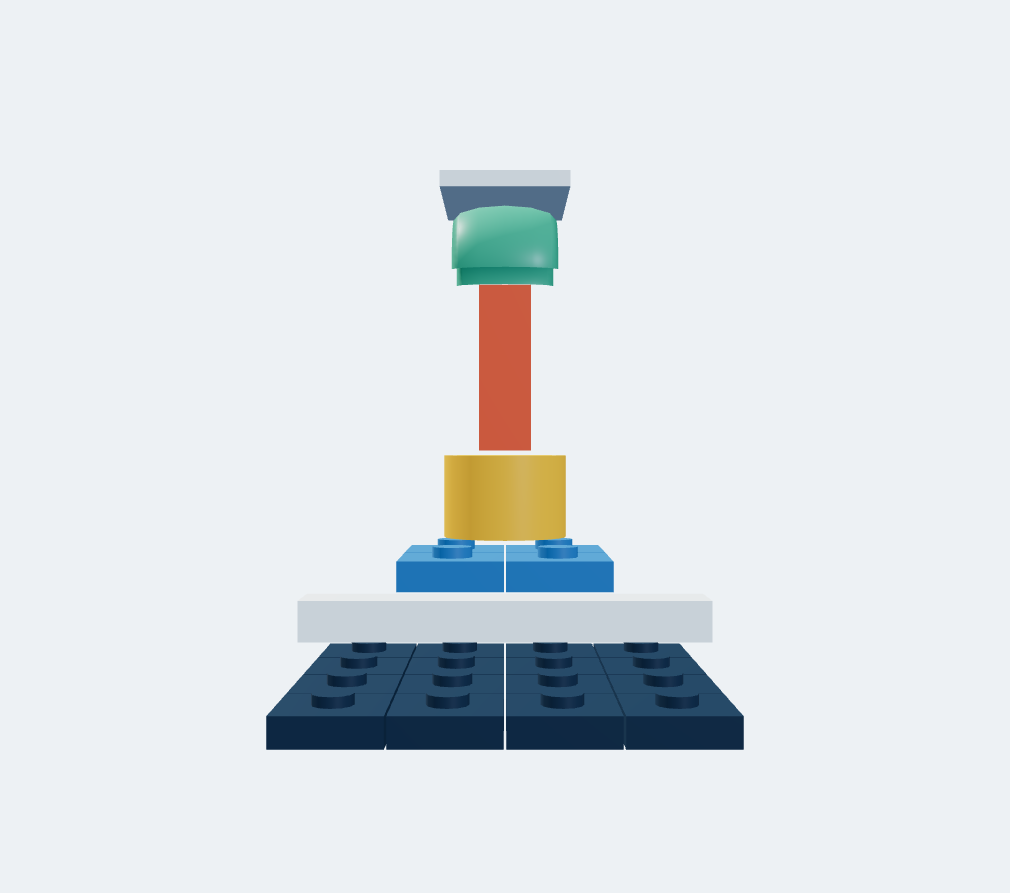
\includegraphics[width=.24\textwidth]{figures/hierarchy-expanded/indexed-toggle-latch-side.png}
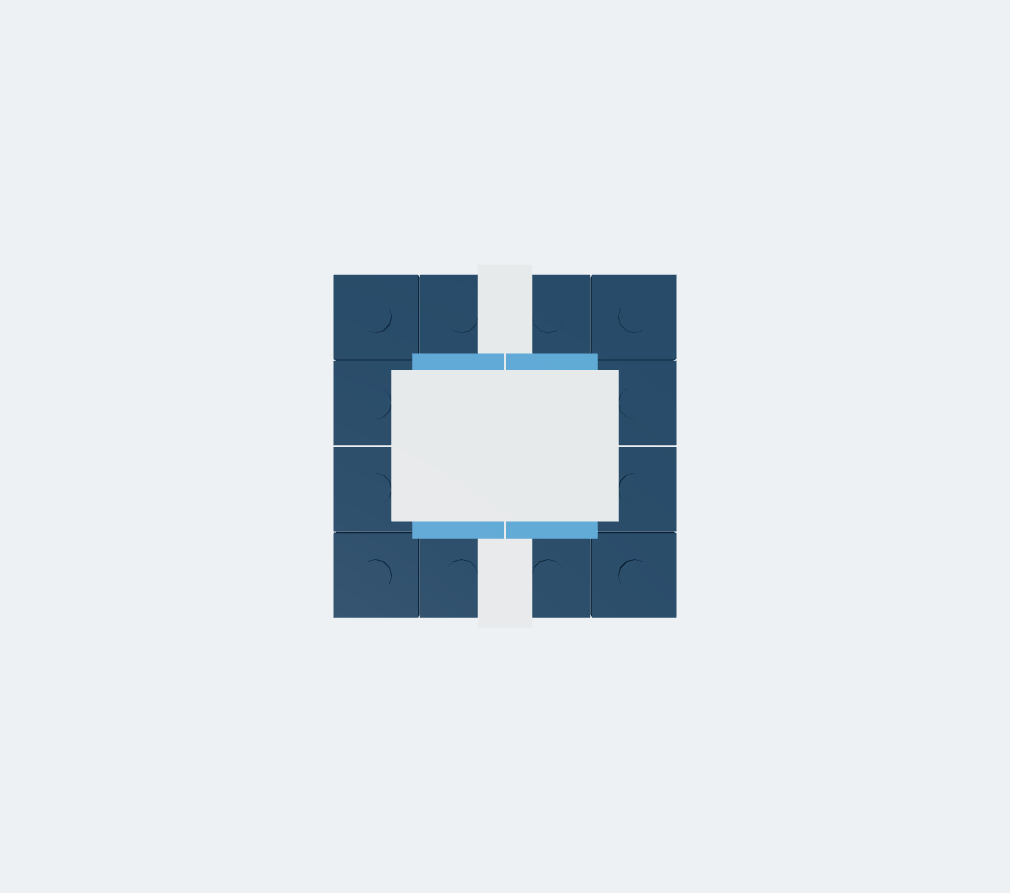
\includegraphics[width=.24\textwidth]{figures/hierarchy-expanded/indexed-toggle-latch-top.png}
\end{center}
\noindent All 48 families share this source. Full inputs and answers appear in the companion question bank.
\begin{center}\tiny\begin{tabular}{rllll}\toprule No. & Family & Layer & Output & Evidence\\\midrule
1 & identify & atomic & single-choice & model-state \\
2 & count & atomic & single-choice & model-state \\
3 & color & atomic & single-choice & model-state \\
4 & position & atomic & single-choice & model-state \\
5 & joint-type & atomic & single-choice & model-state \\
6 & parent & atomic & single-choice & model-state \\
7 & anchor & atomic & single-choice & model-state \\
8 & degree & atomic & single-choice & model-state \\
9 & recolor & atomic & single-choice & model-state \\
10 & add & atomic & single-choice & model-state \\
11 & remove & atomic & single-choice & model-state \\
12 & replace & atomic & single-choice & model-state \\
13 & translate & atomic & single-choice & model-state \\
14 & rotate & atomic & single-choice & model-state \\
15 & next-module & atomic & single-choice & model-state \\
16 & inventory & atomic & single-choice & model-state \\
17 & boundary & atomic & single-choice & model-state \\
18 & no-op & atomic & single-choice & model-state \\
19 & prefix & metacognitive & single-choice & support-graph \\
20 & access & metacognitive & multiple-choice & Rapier \\
21 & counterfactual & metacognitive & single-choice & support-graph \\
22 & dynamic & metacognitive & single-choice & Rapier \\
23 & kinematic & metacognitive & multiple-choice & model-state \\
24 & diagnosis & metacognitive & multiple-choice & model-state \\
25 & information-gain & metacognitive & multiple-choice & finite-world \\
26 & abstention & metacognitive & single-choice & finite-world \\
27 & posterior & metacognitive & single-choice & finite-world \\
28 & pareto & metacognitive & multiple-choice & model-state \\
29 & assembly & procedural & actions & state-machine \\
30 & disassembly & procedural & actions & state-machine \\
31 & service-repair & procedural & actions & state-machine \\
32 & compound-edit & procedural & actions & state-machine \\
33 & multi-fault & integrative & actions & state-machine \\
34 & scheduling & integrative & schedule & resource-schedule \\
35 & policy & integrative & policy & finite-world \\
36 & local-frame & atomic & single-choice & model-state \\
37 & projection & atomic & single-choice & model-state \\
38 & relative-order & atomic & single-choice & model-state \\
39 & joint-axis & atomic & single-choice & model-state \\
40 & clearance-margin & metacognitive & single-choice & model-state \\
41 & load-moment & metacognitive & single-choice & model-state \\
42 & weighted-posterior & metacognitive & single-choice & finite-world \\
43 & expected-loss & metacognitive & single-choice & finite-world \\
44 & trace-threshold & metacognitive & single-choice & Rapier \\
45 & guarded-repair & procedural & actions & state-machine \\
46 & rollback & procedural & actions & state-machine \\
47 & resource-repair & integrative & actions & state-machine \\
48 & budget-policy & integrative & policy & finite-world \\
\bottomrule\end{tabular}\end{center}
\clearpage
\subsection{29. Maintenance Trolley (D1)}
21 visible parts; 5 modules; 4 joints. Representative-point motion 0.0000; rotation 0.0000 rad.
\begin{center}

\includegraphics[width=.24\textwidth]{figures/hierarchy-expanded/maintenance-trolley-iso.png}

\includegraphics[width=.24\textwidth]{figures/hierarchy-expanded/maintenance-trolley-front.png}

\includegraphics[width=.24\textwidth]{figures/hierarchy-expanded/maintenance-trolley-side.png}

\includegraphics[width=.24\textwidth]{figures/hierarchy-expanded/maintenance-trolley-top.png}
\end{center}
\noindent All 48 families share this source. Full inputs and answers appear in the companion question bank.
\begin{center}\tiny\begin{tabular}{rllll}\toprule No. & Family & Layer & Output & Evidence\\\midrule
1 & identify & atomic & single-choice & model-state \\
2 & count & atomic & single-choice & model-state \\
3 & color & atomic & single-choice & model-state \\
4 & position & atomic & single-choice & model-state \\
5 & joint-type & atomic & single-choice & model-state \\
6 & parent & atomic & single-choice & model-state \\
7 & anchor & atomic & single-choice & model-state \\
8 & degree & atomic & single-choice & model-state \\
9 & recolor & atomic & single-choice & model-state \\
10 & add & atomic & single-choice & model-state \\
11 & remove & atomic & single-choice & model-state \\
12 & replace & atomic & single-choice & model-state \\
13 & translate & atomic & single-choice & model-state \\
14 & rotate & atomic & single-choice & model-state \\
15 & next-module & atomic & single-choice & model-state \\
16 & inventory & atomic & single-choice & model-state \\
17 & boundary & atomic & single-choice & model-state \\
18 & no-op & atomic & single-choice & model-state \\
19 & prefix & metacognitive & single-choice & support-graph \\
20 & access & metacognitive & multiple-choice & Rapier \\
21 & counterfactual & metacognitive & single-choice & support-graph \\
22 & dynamic & metacognitive & single-choice & Rapier \\
23 & kinematic & metacognitive & multiple-choice & model-state \\
24 & diagnosis & metacognitive & multiple-choice & model-state \\
25 & information-gain & metacognitive & multiple-choice & finite-world \\
26 & abstention & metacognitive & single-choice & finite-world \\
27 & posterior & metacognitive & single-choice & finite-world \\
28 & pareto & metacognitive & multiple-choice & model-state \\
29 & assembly & procedural & actions & state-machine \\
30 & disassembly & procedural & actions & state-machine \\
31 & service-repair & procedural & actions & state-machine \\
32 & compound-edit & procedural & actions & state-machine \\
33 & multi-fault & integrative & actions & state-machine \\
34 & scheduling & integrative & schedule & resource-schedule \\
35 & policy & integrative & policy & finite-world \\
36 & local-frame & atomic & single-choice & model-state \\
37 & projection & atomic & single-choice & model-state \\
38 & relative-order & atomic & single-choice & model-state \\
39 & joint-axis & atomic & single-choice & model-state \\
40 & clearance-margin & metacognitive & single-choice & model-state \\
41 & load-moment & metacognitive & single-choice & model-state \\
42 & weighted-posterior & metacognitive & single-choice & finite-world \\
43 & expected-loss & metacognitive & single-choice & finite-world \\
44 & trace-threshold & metacognitive & single-choice & Rapier \\
45 & guarded-repair & procedural & actions & state-machine \\
46 & rollback & procedural & actions & state-machine \\
47 & resource-repair & integrative & actions & state-machine \\
48 & budget-policy & integrative & policy & finite-world \\
\bottomrule\end{tabular}\end{center}
\clearpage
\subsection{30. Orthogonal Probe Stage (D1)}
25 visible parts; 6 modules; 5 joints. Representative-point motion 0.0000; rotation 0.0000 rad.
\begin{center}

\includegraphics[width=.24\textwidth]{figures/hierarchy-expanded/orthogonal-probe-stage-iso.png}
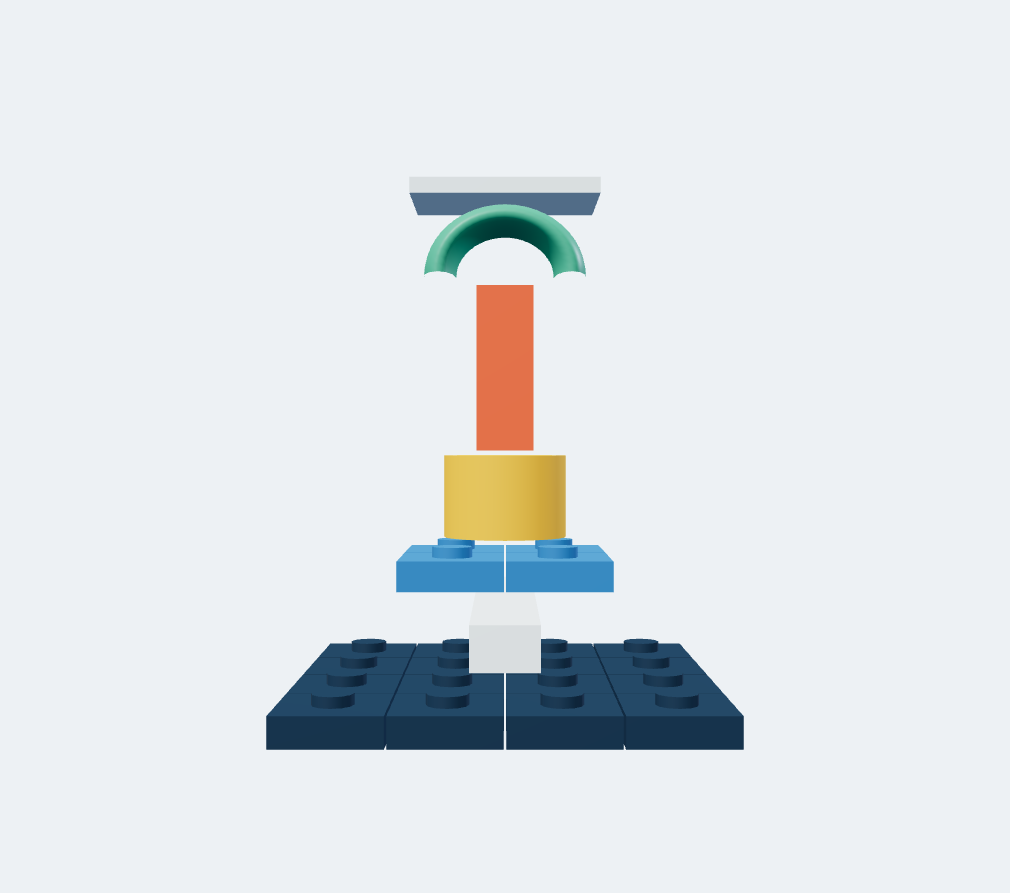
\includegraphics[width=.24\textwidth]{figures/hierarchy-expanded/orthogonal-probe-stage-front.png}
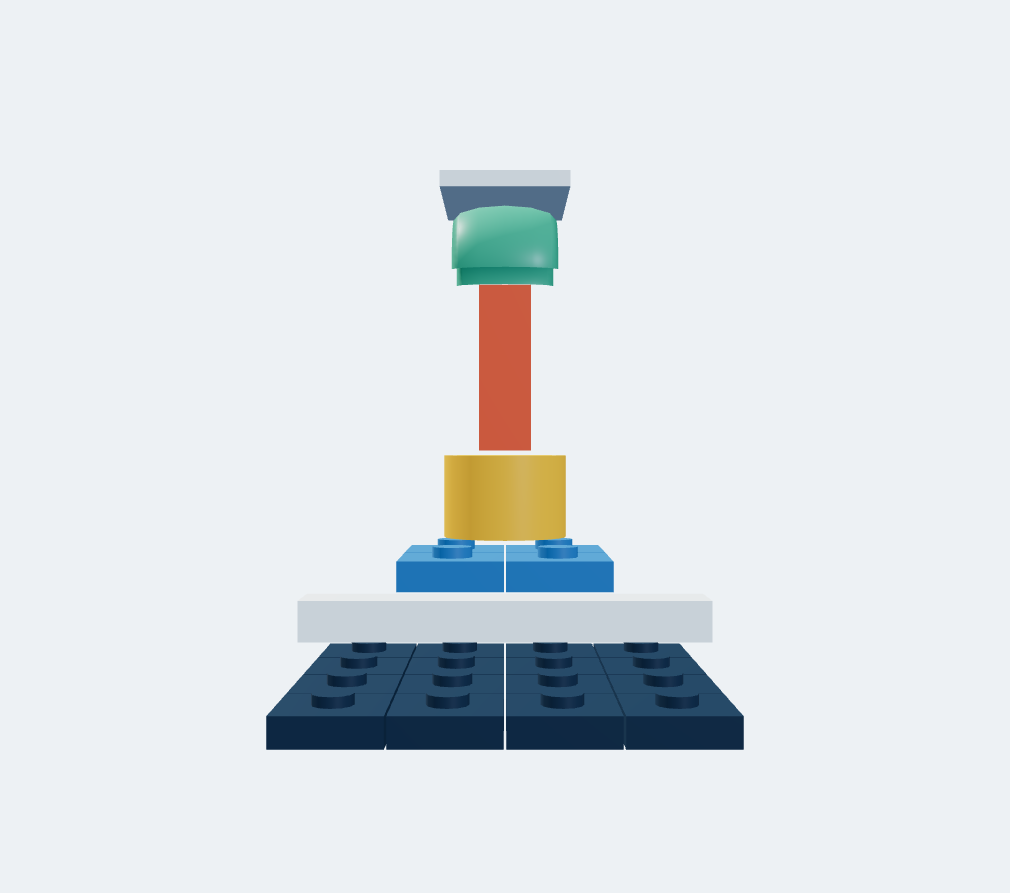
\includegraphics[width=.24\textwidth]{figures/hierarchy-expanded/orthogonal-probe-stage-side.png}
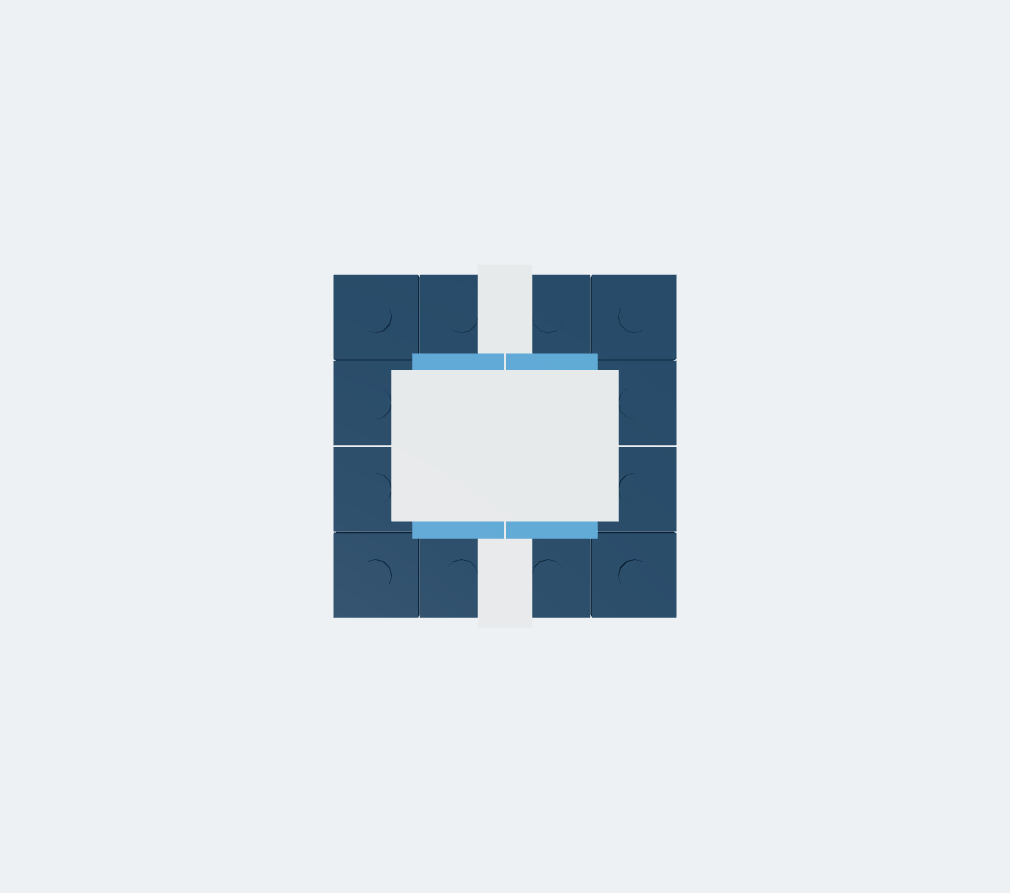
\includegraphics[width=.24\textwidth]{figures/hierarchy-expanded/orthogonal-probe-stage-top.png}
\end{center}
\noindent All 48 families share this source. Full inputs and answers appear in the companion question bank.
\begin{center}\tiny\begin{tabular}{rllll}\toprule No. & Family & Layer & Output & Evidence\\\midrule
1 & identify & atomic & single-choice & model-state \\
2 & count & atomic & single-choice & model-state \\
3 & color & atomic & single-choice & model-state \\
4 & position & atomic & single-choice & model-state \\
5 & joint-type & atomic & single-choice & model-state \\
6 & parent & atomic & single-choice & model-state \\
7 & anchor & atomic & single-choice & model-state \\
8 & degree & atomic & single-choice & model-state \\
9 & recolor & atomic & single-choice & model-state \\
10 & add & atomic & single-choice & model-state \\
11 & remove & atomic & single-choice & model-state \\
12 & replace & atomic & single-choice & model-state \\
13 & translate & atomic & single-choice & model-state \\
14 & rotate & atomic & single-choice & model-state \\
15 & next-module & atomic & single-choice & model-state \\
16 & inventory & atomic & single-choice & model-state \\
17 & boundary & atomic & single-choice & model-state \\
18 & no-op & atomic & single-choice & model-state \\
19 & prefix & metacognitive & single-choice & support-graph \\
20 & access & metacognitive & multiple-choice & Rapier \\
21 & counterfactual & metacognitive & single-choice & support-graph \\
22 & dynamic & metacognitive & single-choice & Rapier \\
23 & kinematic & metacognitive & multiple-choice & model-state \\
24 & diagnosis & metacognitive & multiple-choice & model-state \\
25 & information-gain & metacognitive & multiple-choice & finite-world \\
26 & abstention & metacognitive & single-choice & finite-world \\
27 & posterior & metacognitive & single-choice & finite-world \\
28 & pareto & metacognitive & multiple-choice & model-state \\
29 & assembly & procedural & actions & state-machine \\
30 & disassembly & procedural & actions & state-machine \\
31 & service-repair & procedural & actions & state-machine \\
32 & compound-edit & procedural & actions & state-machine \\
33 & multi-fault & integrative & actions & state-machine \\
34 & scheduling & integrative & schedule & resource-schedule \\
35 & policy & integrative & policy & finite-world \\
36 & local-frame & atomic & single-choice & model-state \\
37 & projection & atomic & single-choice & model-state \\
38 & relative-order & atomic & single-choice & model-state \\
39 & joint-axis & atomic & single-choice & model-state \\
40 & clearance-margin & metacognitive & single-choice & model-state \\
41 & load-moment & metacognitive & single-choice & model-state \\
42 & weighted-posterior & metacognitive & single-choice & finite-world \\
43 & expected-loss & metacognitive & single-choice & finite-world \\
44 & trace-threshold & metacognitive & single-choice & Rapier \\
45 & guarded-repair & procedural & actions & state-machine \\
46 & rollback & procedural & actions & state-machine \\
47 & resource-repair & integrative & actions & state-machine \\
48 & budget-policy & integrative & policy & finite-world \\
\bottomrule\end{tabular}\end{center}
\clearpage
\subsection{31. Ratchet Hoist (D1)}
16 visible parts; 4 modules; 3 joints. Representative-point motion 0.0006; rotation 0.0000 rad.
\begin{center}

\includegraphics[width=.24\textwidth]{figures/hierarchy-expanded/ratchet-hoist-iso.png}

\includegraphics[width=.24\textwidth]{figures/hierarchy-expanded/ratchet-hoist-front.png}

\includegraphics[width=.24\textwidth]{figures/hierarchy-expanded/ratchet-hoist-side.png}

\includegraphics[width=.24\textwidth]{figures/hierarchy-expanded/ratchet-hoist-top.png}
\end{center}
\noindent All 48 families share this source. Full inputs and answers appear in the companion question bank.
\begin{center}\tiny\begin{tabular}{rllll}\toprule No. & Family & Layer & Output & Evidence\\\midrule
1 & identify & atomic & single-choice & model-state \\
2 & count & atomic & single-choice & model-state \\
3 & color & atomic & single-choice & model-state \\
4 & position & atomic & single-choice & model-state \\
5 & joint-type & atomic & single-choice & model-state \\
6 & parent & atomic & single-choice & model-state \\
7 & anchor & atomic & single-choice & model-state \\
8 & degree & atomic & single-choice & model-state \\
9 & recolor & atomic & single-choice & model-state \\
10 & add & atomic & single-choice & model-state \\
11 & remove & atomic & single-choice & model-state \\
12 & replace & atomic & single-choice & model-state \\
13 & translate & atomic & single-choice & model-state \\
14 & rotate & atomic & single-choice & model-state \\
15 & next-module & atomic & single-choice & model-state \\
16 & inventory & atomic & single-choice & model-state \\
17 & boundary & atomic & single-choice & model-state \\
18 & no-op & atomic & single-choice & model-state \\
19 & prefix & metacognitive & single-choice & support-graph \\
20 & access & metacognitive & multiple-choice & Rapier \\
21 & counterfactual & metacognitive & single-choice & support-graph \\
22 & dynamic & metacognitive & single-choice & Rapier \\
23 & kinematic & metacognitive & multiple-choice & model-state \\
24 & diagnosis & metacognitive & multiple-choice & model-state \\
25 & information-gain & metacognitive & multiple-choice & finite-world \\
26 & abstention & metacognitive & single-choice & finite-world \\
27 & posterior & metacognitive & single-choice & finite-world \\
28 & pareto & metacognitive & multiple-choice & model-state \\
29 & assembly & procedural & actions & state-machine \\
30 & disassembly & procedural & actions & state-machine \\
31 & service-repair & procedural & actions & state-machine \\
32 & compound-edit & procedural & actions & state-machine \\
33 & multi-fault & integrative & actions & state-machine \\
34 & scheduling & integrative & schedule & resource-schedule \\
35 & policy & integrative & policy & finite-world \\
36 & local-frame & atomic & single-choice & model-state \\
37 & projection & atomic & single-choice & model-state \\
38 & relative-order & atomic & single-choice & model-state \\
39 & joint-axis & atomic & single-choice & model-state \\
40 & clearance-margin & metacognitive & single-choice & model-state \\
41 & load-moment & metacognitive & single-choice & model-state \\
42 & weighted-posterior & metacognitive & single-choice & finite-world \\
43 & expected-loss & metacognitive & single-choice & finite-world \\
44 & trace-threshold & metacognitive & single-choice & Rapier \\
45 & guarded-repair & procedural & actions & state-machine \\
46 & rollback & procedural & actions & state-machine \\
47 & resource-repair & integrative & actions & state-machine \\
48 & budget-policy & integrative & policy & finite-world \\
\bottomrule\end{tabular}\end{center}
\clearpage
\subsection{32. Sample Carousel (D1)}
15 visible parts; 4 modules; 3 joints. Representative-point motion 0.0000; rotation 0.0000 rad.
\begin{center}

\includegraphics[width=.24\textwidth]{figures/hierarchy-expanded/sample-carousel-iso.png}

\includegraphics[width=.24\textwidth]{figures/hierarchy-expanded/sample-carousel-front.png}

\includegraphics[width=.24\textwidth]{figures/hierarchy-expanded/sample-carousel-side.png}

\includegraphics[width=.24\textwidth]{figures/hierarchy-expanded/sample-carousel-top.png}
\end{center}
\noindent All 48 families share this source. Full inputs and answers appear in the companion question bank.
\begin{center}\tiny\begin{tabular}{rllll}\toprule No. & Family & Layer & Output & Evidence\\\midrule
1 & identify & atomic & single-choice & model-state \\
2 & count & atomic & single-choice & model-state \\
3 & color & atomic & single-choice & model-state \\
4 & position & atomic & single-choice & model-state \\
5 & joint-type & atomic & single-choice & model-state \\
6 & parent & atomic & single-choice & model-state \\
7 & anchor & atomic & single-choice & model-state \\
8 & degree & atomic & single-choice & model-state \\
9 & recolor & atomic & single-choice & model-state \\
10 & add & atomic & single-choice & model-state \\
11 & remove & atomic & single-choice & model-state \\
12 & replace & atomic & single-choice & model-state \\
13 & translate & atomic & single-choice & model-state \\
14 & rotate & atomic & single-choice & model-state \\
15 & next-module & atomic & single-choice & model-state \\
16 & inventory & atomic & single-choice & model-state \\
17 & boundary & atomic & single-choice & model-state \\
18 & no-op & atomic & single-choice & model-state \\
19 & prefix & metacognitive & single-choice & support-graph \\
20 & access & metacognitive & multiple-choice & Rapier \\
21 & counterfactual & metacognitive & single-choice & support-graph \\
22 & dynamic & metacognitive & single-choice & Rapier \\
23 & kinematic & metacognitive & multiple-choice & model-state \\
24 & diagnosis & metacognitive & multiple-choice & model-state \\
25 & information-gain & metacognitive & multiple-choice & finite-world \\
26 & abstention & metacognitive & single-choice & finite-world \\
27 & posterior & metacognitive & single-choice & finite-world \\
28 & pareto & metacognitive & multiple-choice & model-state \\
29 & assembly & procedural & actions & state-machine \\
30 & disassembly & procedural & actions & state-machine \\
31 & service-repair & procedural & actions & state-machine \\
32 & compound-edit & procedural & actions & state-machine \\
33 & multi-fault & integrative & actions & state-machine \\
34 & scheduling & integrative & schedule & resource-schedule \\
35 & policy & integrative & policy & finite-world \\
36 & local-frame & atomic & single-choice & model-state \\
37 & projection & atomic & single-choice & model-state \\
38 & relative-order & atomic & single-choice & model-state \\
39 & joint-axis & atomic & single-choice & model-state \\
40 & clearance-margin & metacognitive & single-choice & model-state \\
41 & load-moment & metacognitive & single-choice & model-state \\
42 & weighted-posterior & metacognitive & single-choice & finite-world \\
43 & expected-loss & metacognitive & single-choice & finite-world \\
44 & trace-threshold & metacognitive & single-choice & Rapier \\
45 & guarded-repair & procedural & actions & state-machine \\
46 & rollback & procedural & actions & state-machine \\
47 & resource-repair & integrative & actions & state-machine \\
48 & budget-policy & integrative & policy & finite-world \\
\bottomrule\end{tabular}\end{center}
\clearpage
\subsection{33. Signal Switch Stand (D1)}
22 visible parts; 4 modules; 3 joints. Representative-point motion 0.0035; rotation 0.0000 rad.
\begin{center}

\includegraphics[width=.24\textwidth]{figures/hierarchy-expanded/signal-switch-stand-iso.png}

\includegraphics[width=.24\textwidth]{figures/hierarchy-expanded/signal-switch-stand-front.png}

\includegraphics[width=.24\textwidth]{figures/hierarchy-expanded/signal-switch-stand-side.png}

\includegraphics[width=.24\textwidth]{figures/hierarchy-expanded/signal-switch-stand-top.png}
\end{center}
\noindent All 48 families share this source. Full inputs and answers appear in the companion question bank.
\begin{center}\tiny\begin{tabular}{rllll}\toprule No. & Family & Layer & Output & Evidence\\\midrule
1 & identify & atomic & single-choice & model-state \\
2 & count & atomic & single-choice & model-state \\
3 & color & atomic & single-choice & model-state \\
4 & position & atomic & single-choice & model-state \\
5 & joint-type & atomic & single-choice & model-state \\
6 & parent & atomic & single-choice & model-state \\
7 & anchor & atomic & single-choice & model-state \\
8 & degree & atomic & single-choice & model-state \\
9 & recolor & atomic & single-choice & model-state \\
10 & add & atomic & single-choice & model-state \\
11 & remove & atomic & single-choice & model-state \\
12 & replace & atomic & single-choice & model-state \\
13 & translate & atomic & single-choice & model-state \\
14 & rotate & atomic & single-choice & model-state \\
15 & next-module & atomic & single-choice & model-state \\
16 & inventory & atomic & single-choice & model-state \\
17 & boundary & atomic & single-choice & model-state \\
18 & no-op & atomic & single-choice & model-state \\
19 & prefix & metacognitive & single-choice & support-graph \\
20 & access & metacognitive & multiple-choice & Rapier \\
21 & counterfactual & metacognitive & single-choice & support-graph \\
22 & dynamic & metacognitive & single-choice & Rapier \\
23 & kinematic & metacognitive & multiple-choice & model-state \\
24 & diagnosis & metacognitive & multiple-choice & model-state \\
25 & information-gain & metacognitive & multiple-choice & finite-world \\
26 & abstention & metacognitive & single-choice & finite-world \\
27 & posterior & metacognitive & single-choice & finite-world \\
28 & pareto & metacognitive & multiple-choice & model-state \\
29 & assembly & procedural & actions & state-machine \\
30 & disassembly & procedural & actions & state-machine \\
31 & service-repair & procedural & actions & state-machine \\
32 & compound-edit & procedural & actions & state-machine \\
33 & multi-fault & integrative & actions & state-machine \\
34 & scheduling & integrative & schedule & resource-schedule \\
35 & policy & integrative & policy & finite-world \\
36 & local-frame & atomic & single-choice & model-state \\
37 & projection & atomic & single-choice & model-state \\
38 & relative-order & atomic & single-choice & model-state \\
39 & joint-axis & atomic & single-choice & model-state \\
40 & clearance-margin & metacognitive & single-choice & model-state \\
41 & load-moment & metacognitive & single-choice & model-state \\
42 & weighted-posterior & metacognitive & single-choice & finite-world \\
43 & expected-loss & metacognitive & single-choice & finite-world \\
44 & trace-threshold & metacognitive & single-choice & Rapier \\
45 & guarded-repair & procedural & actions & state-machine \\
46 & rollback & procedural & actions & state-machine \\
47 & resource-repair & integrative & actions & state-machine \\
48 & budget-policy & integrative & policy & finite-world \\
\bottomrule\end{tabular}\end{center}
\clearpage
\subsection{34. Rail Tool Drawer (D1)}
17 visible parts; 4 modules; 3 joints. Representative-point motion 0.0000; rotation 0.0000 rad.
\begin{center}

\includegraphics[width=.24\textwidth]{figures/hierarchy-expanded/sliding-drawer-iso.png}

\includegraphics[width=.24\textwidth]{figures/hierarchy-expanded/sliding-drawer-front.png}

\includegraphics[width=.24\textwidth]{figures/hierarchy-expanded/sliding-drawer-side.png}

\includegraphics[width=.24\textwidth]{figures/hierarchy-expanded/sliding-drawer-top.png}
\end{center}
\noindent All 48 families share this source. Full inputs and answers appear in the companion question bank.
\begin{center}\tiny\begin{tabular}{rllll}\toprule No. & Family & Layer & Output & Evidence\\\midrule
1 & identify & atomic & single-choice & model-state \\
2 & count & atomic & single-choice & model-state \\
3 & color & atomic & single-choice & model-state \\
4 & position & atomic & single-choice & model-state \\
5 & joint-type & atomic & single-choice & model-state \\
6 & parent & atomic & single-choice & model-state \\
7 & anchor & atomic & single-choice & model-state \\
8 & degree & atomic & single-choice & model-state \\
9 & recolor & atomic & single-choice & model-state \\
10 & add & atomic & single-choice & model-state \\
11 & remove & atomic & single-choice & model-state \\
12 & replace & atomic & single-choice & model-state \\
13 & translate & atomic & single-choice & model-state \\
14 & rotate & atomic & single-choice & model-state \\
15 & next-module & atomic & single-choice & model-state \\
16 & inventory & atomic & single-choice & model-state \\
17 & boundary & atomic & single-choice & model-state \\
18 & no-op & atomic & single-choice & model-state \\
19 & prefix & metacognitive & single-choice & support-graph \\
20 & access & metacognitive & multiple-choice & Rapier \\
21 & counterfactual & metacognitive & single-choice & support-graph \\
22 & dynamic & metacognitive & single-choice & Rapier \\
23 & kinematic & metacognitive & multiple-choice & model-state \\
24 & diagnosis & metacognitive & multiple-choice & model-state \\
25 & information-gain & metacognitive & multiple-choice & finite-world \\
26 & abstention & metacognitive & single-choice & finite-world \\
27 & posterior & metacognitive & single-choice & finite-world \\
28 & pareto & metacognitive & multiple-choice & model-state \\
29 & assembly & procedural & actions & state-machine \\
30 & disassembly & procedural & actions & state-machine \\
31 & service-repair & procedural & actions & state-machine \\
32 & compound-edit & procedural & actions & state-machine \\
33 & multi-fault & integrative & actions & state-machine \\
34 & scheduling & integrative & schedule & resource-schedule \\
35 & policy & integrative & policy & finite-world \\
36 & local-frame & atomic & single-choice & model-state \\
37 & projection & atomic & single-choice & model-state \\
38 & relative-order & atomic & single-choice & model-state \\
39 & joint-axis & atomic & single-choice & model-state \\
40 & clearance-margin & metacognitive & single-choice & model-state \\
41 & load-moment & metacognitive & single-choice & model-state \\
42 & weighted-posterior & metacognitive & single-choice & finite-world \\
43 & expected-loss & metacognitive & single-choice & finite-world \\
44 & trace-threshold & metacognitive & single-choice & Rapier \\
45 & guarded-repair & procedural & actions & state-machine \\
46 & rollback & procedural & actions & state-machine \\
47 & resource-repair & integrative & actions & state-machine \\
48 & budget-policy & integrative & policy & finite-world \\
\bottomrule\end{tabular}\end{center}
\clearpage
\subsection{35. Valve Control Stand (D1)}
25 visible parts; 3 modules; 2 joints. Representative-point motion 0.0000; rotation 0.0000 rad.
\begin{center}

\includegraphics[width=.24\textwidth]{figures/hierarchy-expanded/valve-control-stand-iso.png}

\includegraphics[width=.24\textwidth]{figures/hierarchy-expanded/valve-control-stand-front.png}

\includegraphics[width=.24\textwidth]{figures/hierarchy-expanded/valve-control-stand-side.png}

\includegraphics[width=.24\textwidth]{figures/hierarchy-expanded/valve-control-stand-top.png}
\end{center}
\noindent All 48 families share this source. Full inputs and answers appear in the companion question bank.
\begin{center}\tiny\begin{tabular}{rllll}\toprule No. & Family & Layer & Output & Evidence\\\midrule
1 & identify & atomic & single-choice & model-state \\
2 & count & atomic & single-choice & model-state \\
3 & color & atomic & single-choice & model-state \\
4 & position & atomic & single-choice & model-state \\
5 & joint-type & atomic & single-choice & model-state \\
6 & parent & atomic & single-choice & model-state \\
7 & anchor & atomic & single-choice & model-state \\
8 & degree & atomic & single-choice & model-state \\
9 & recolor & atomic & single-choice & model-state \\
10 & add & atomic & single-choice & model-state \\
11 & remove & atomic & single-choice & model-state \\
12 & replace & atomic & single-choice & model-state \\
13 & translate & atomic & single-choice & model-state \\
14 & rotate & atomic & single-choice & model-state \\
15 & next-module & atomic & single-choice & model-state \\
16 & inventory & atomic & single-choice & model-state \\
17 & boundary & atomic & single-choice & model-state \\
18 & no-op & atomic & single-choice & model-state \\
19 & prefix & metacognitive & single-choice & support-graph \\
20 & access & metacognitive & multiple-choice & Rapier \\
21 & counterfactual & metacognitive & single-choice & support-graph \\
22 & dynamic & metacognitive & single-choice & Rapier \\
23 & kinematic & metacognitive & multiple-choice & model-state \\
24 & diagnosis & metacognitive & multiple-choice & model-state \\
25 & information-gain & metacognitive & multiple-choice & finite-world \\
26 & abstention & metacognitive & single-choice & finite-world \\
27 & posterior & metacognitive & single-choice & finite-world \\
28 & pareto & metacognitive & multiple-choice & model-state \\
29 & assembly & procedural & actions & state-machine \\
30 & disassembly & procedural & actions & state-machine \\
31 & service-repair & procedural & actions & state-machine \\
32 & compound-edit & procedural & actions & state-machine \\
33 & multi-fault & integrative & actions & state-machine \\
34 & scheduling & integrative & schedule & resource-schedule \\
35 & policy & integrative & policy & finite-world \\
36 & local-frame & atomic & single-choice & model-state \\
37 & projection & atomic & single-choice & model-state \\
38 & relative-order & atomic & single-choice & model-state \\
39 & joint-axis & atomic & single-choice & model-state \\
40 & clearance-margin & metacognitive & single-choice & model-state \\
41 & load-moment & metacognitive & single-choice & model-state \\
42 & weighted-posterior & metacognitive & single-choice & finite-world \\
43 & expected-loss & metacognitive & single-choice & finite-world \\
44 & trace-threshold & metacognitive & single-choice & Rapier \\
45 & guarded-repair & procedural & actions & state-machine \\
46 & rollback & procedural & actions & state-machine \\
47 & resource-repair & integrative & actions & state-machine \\
48 & budget-policy & integrative & policy & finite-world \\
\bottomrule\end{tabular}\end{center}
\clearpage
\subsection{36. Wind Vane (D1)}
14 visible parts; 4 modules; 3 joints. Representative-point motion 0.0000; rotation 0.0000 rad.
\begin{center}

\includegraphics[width=.24\textwidth]{figures/hierarchy-expanded/wind-vane-iso.png}

\includegraphics[width=.24\textwidth]{figures/hierarchy-expanded/wind-vane-front.png}

\includegraphics[width=.24\textwidth]{figures/hierarchy-expanded/wind-vane-side.png}

\includegraphics[width=.24\textwidth]{figures/hierarchy-expanded/wind-vane-top.png}
\end{center}
\noindent All 48 families share this source. Full inputs and answers appear in the companion question bank.
\begin{center}\tiny\begin{tabular}{rllll}\toprule No. & Family & Layer & Output & Evidence\\\midrule
1 & identify & atomic & single-choice & model-state \\
2 & count & atomic & single-choice & model-state \\
3 & color & atomic & single-choice & model-state \\
4 & position & atomic & single-choice & model-state \\
5 & joint-type & atomic & single-choice & model-state \\
6 & parent & atomic & single-choice & model-state \\
7 & anchor & atomic & single-choice & model-state \\
8 & degree & atomic & single-choice & model-state \\
9 & recolor & atomic & single-choice & model-state \\
10 & add & atomic & single-choice & model-state \\
11 & remove & atomic & single-choice & model-state \\
12 & replace & atomic & single-choice & model-state \\
13 & translate & atomic & single-choice & model-state \\
14 & rotate & atomic & single-choice & model-state \\
15 & next-module & atomic & single-choice & model-state \\
16 & inventory & atomic & single-choice & model-state \\
17 & boundary & atomic & single-choice & model-state \\
18 & no-op & atomic & single-choice & model-state \\
19 & prefix & metacognitive & single-choice & support-graph \\
20 & access & metacognitive & multiple-choice & Rapier \\
21 & counterfactual & metacognitive & single-choice & support-graph \\
22 & dynamic & metacognitive & single-choice & Rapier \\
23 & kinematic & metacognitive & multiple-choice & model-state \\
24 & diagnosis & metacognitive & multiple-choice & model-state \\
25 & information-gain & metacognitive & multiple-choice & finite-world \\
26 & abstention & metacognitive & single-choice & finite-world \\
27 & posterior & metacognitive & single-choice & finite-world \\
28 & pareto & metacognitive & multiple-choice & model-state \\
29 & assembly & procedural & actions & state-machine \\
30 & disassembly & procedural & actions & state-machine \\
31 & service-repair & procedural & actions & state-machine \\
32 & compound-edit & procedural & actions & state-machine \\
33 & multi-fault & integrative & actions & state-machine \\
34 & scheduling & integrative & schedule & resource-schedule \\
35 & policy & integrative & policy & finite-world \\
36 & local-frame & atomic & single-choice & model-state \\
37 & projection & atomic & single-choice & model-state \\
38 & relative-order & atomic & single-choice & model-state \\
39 & joint-axis & atomic & single-choice & model-state \\
40 & clearance-margin & metacognitive & single-choice & model-state \\
41 & load-moment & metacognitive & single-choice & model-state \\
42 & weighted-posterior & metacognitive & single-choice & finite-world \\
43 & expected-loss & metacognitive & single-choice & finite-world \\
44 & trace-threshold & metacognitive & single-choice & Rapier \\
45 & guarded-repair & procedural & actions & state-machine \\
46 & rollback & procedural & actions & state-machine \\
47 & resource-repair & integrative & actions & state-machine \\
48 & budget-policy & integrative & policy & finite-world \\
\bottomrule\end{tabular}\end{center}
\clearpage
\subsection{37. Articulated Camera Dolly (D2)}
54 visible parts; 11 modules; 10 joints. Representative-point motion 0.0000; rotation 0.0000 rad.
\begin{center}
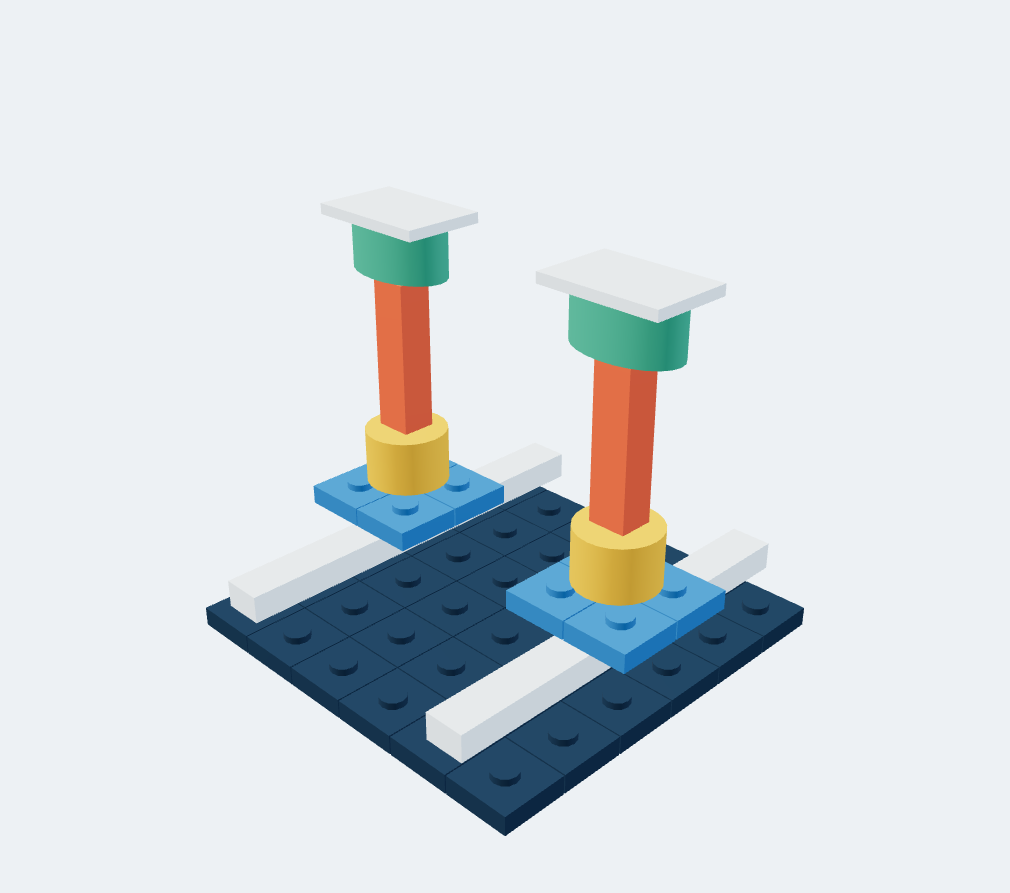
\includegraphics[width=.24\textwidth]{figures/hierarchy-expanded/articulated-camera-dolly-iso.png}
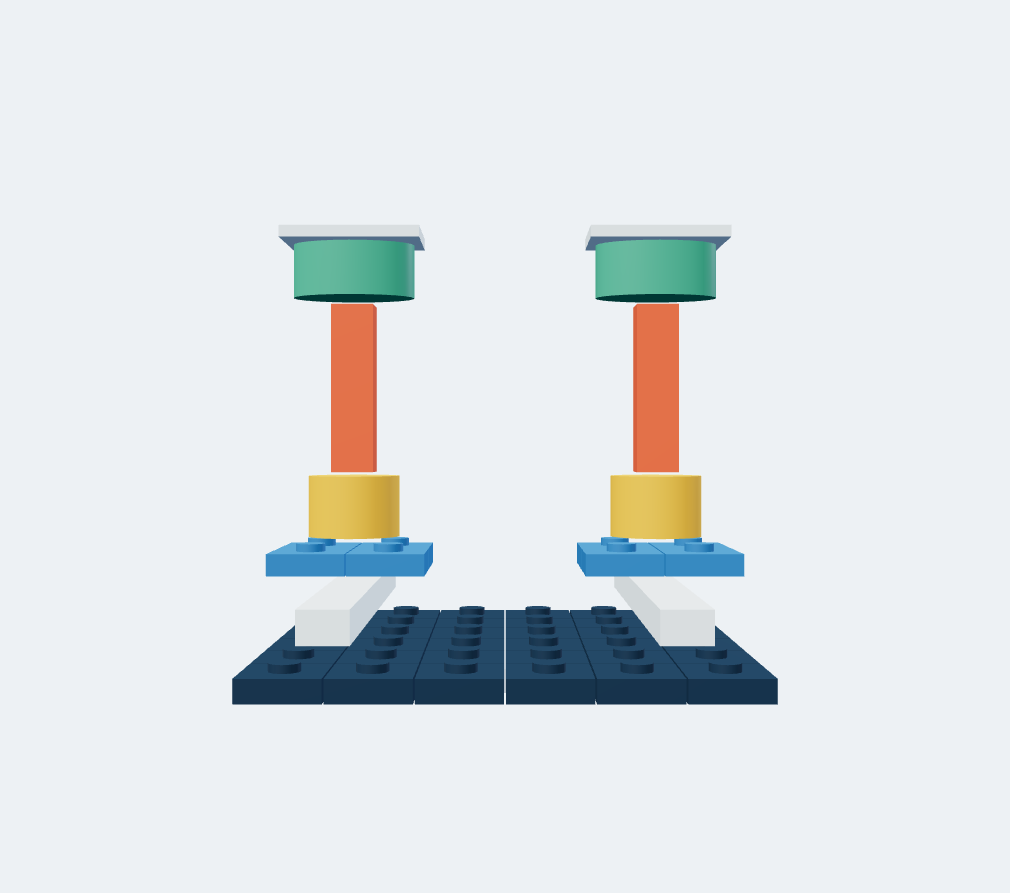
\includegraphics[width=.24\textwidth]{figures/hierarchy-expanded/articulated-camera-dolly-front.png}
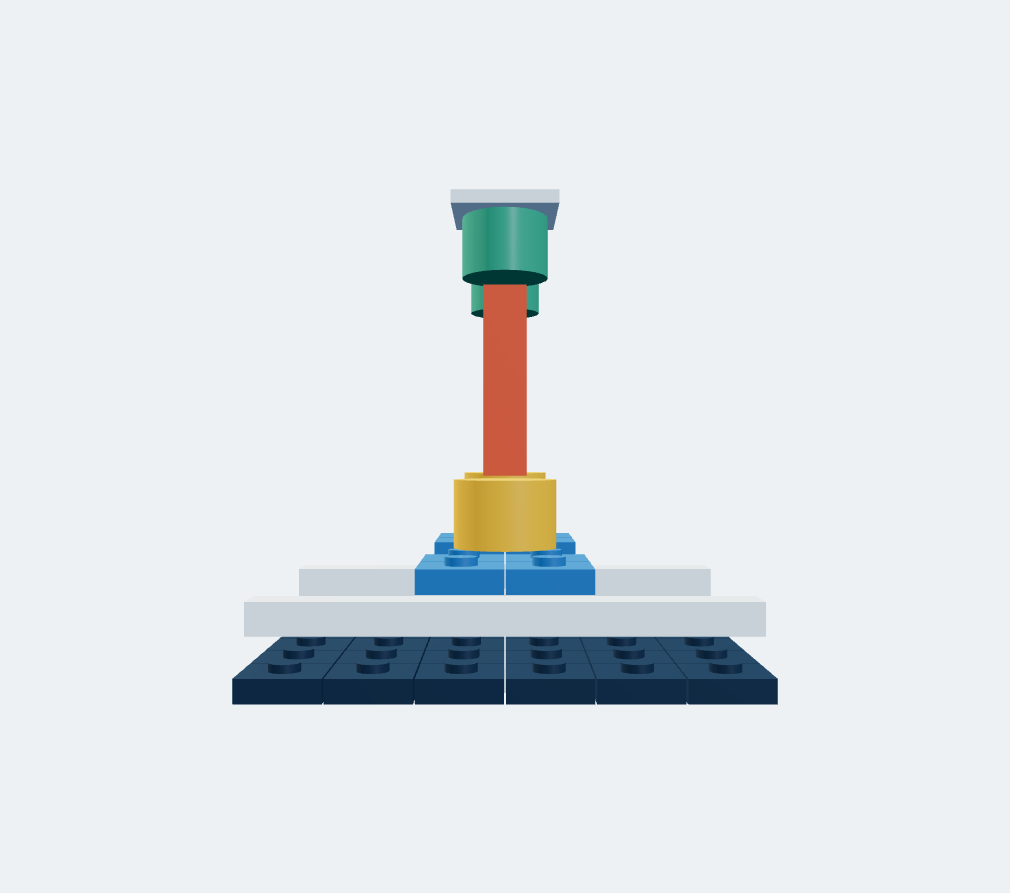
\includegraphics[width=.24\textwidth]{figures/hierarchy-expanded/articulated-camera-dolly-side.png}
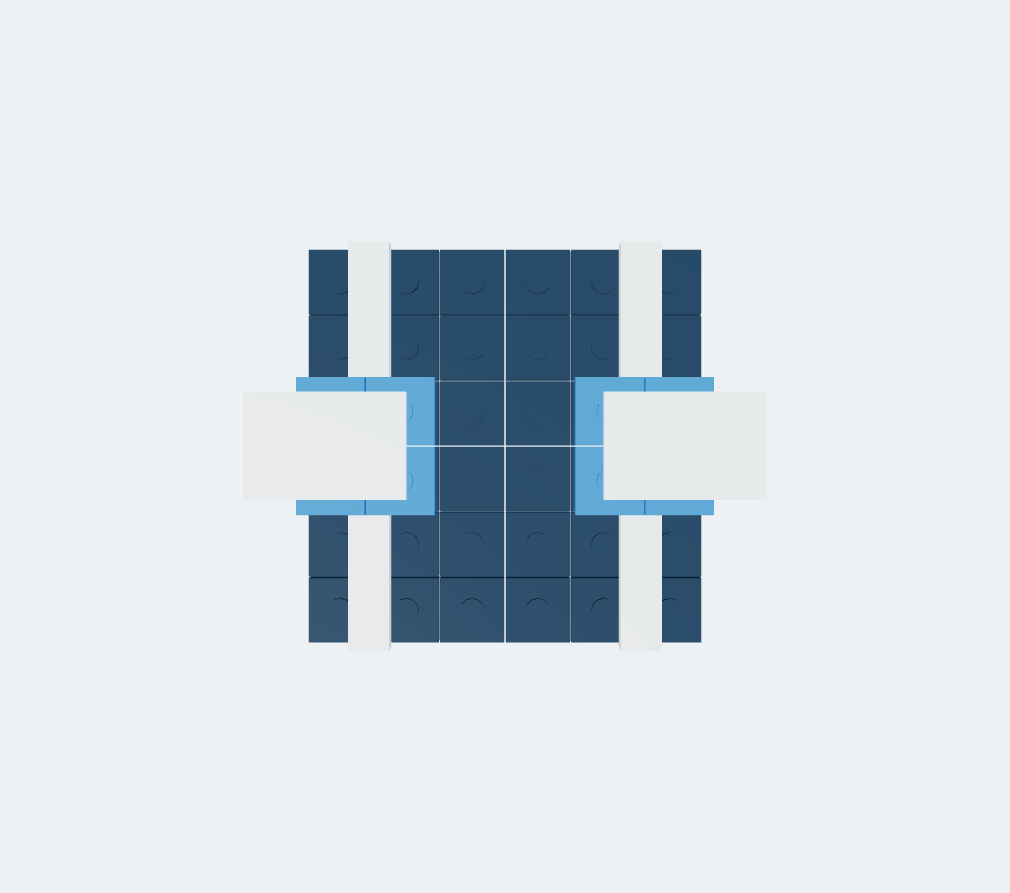
\includegraphics[width=.24\textwidth]{figures/hierarchy-expanded/articulated-camera-dolly-top.png}
\end{center}
\noindent All 48 families share this source. Full inputs and answers appear in the companion question bank.
\begin{center}\tiny\begin{tabular}{rllll}\toprule No. & Family & Layer & Output & Evidence\\\midrule
1 & identify & atomic & single-choice & model-state \\
2 & count & atomic & single-choice & model-state \\
3 & color & atomic & single-choice & model-state \\
4 & position & atomic & single-choice & model-state \\
5 & joint-type & atomic & single-choice & model-state \\
6 & parent & atomic & single-choice & model-state \\
7 & anchor & atomic & single-choice & model-state \\
8 & degree & atomic & single-choice & model-state \\
9 & recolor & atomic & single-choice & model-state \\
10 & add & atomic & single-choice & model-state \\
11 & remove & atomic & single-choice & model-state \\
12 & replace & atomic & single-choice & model-state \\
13 & translate & atomic & single-choice & model-state \\
14 & rotate & atomic & single-choice & model-state \\
15 & next-module & atomic & single-choice & model-state \\
16 & inventory & atomic & single-choice & model-state \\
17 & boundary & atomic & single-choice & model-state \\
18 & no-op & atomic & single-choice & model-state \\
19 & prefix & metacognitive & single-choice & support-graph \\
20 & access & metacognitive & multiple-choice & Rapier \\
21 & counterfactual & metacognitive & single-choice & support-graph \\
22 & dynamic & metacognitive & single-choice & Rapier \\
23 & kinematic & metacognitive & multiple-choice & model-state \\
24 & diagnosis & metacognitive & multiple-choice & model-state \\
25 & information-gain & metacognitive & multiple-choice & finite-world \\
26 & abstention & metacognitive & single-choice & finite-world \\
27 & posterior & metacognitive & single-choice & finite-world \\
28 & pareto & metacognitive & multiple-choice & model-state \\
29 & assembly & procedural & actions & state-machine \\
30 & disassembly & procedural & actions & state-machine \\
31 & service-repair & procedural & actions & state-machine \\
32 & compound-edit & procedural & actions & state-machine \\
33 & multi-fault & integrative & actions & state-machine \\
34 & scheduling & integrative & schedule & resource-schedule \\
35 & policy & integrative & policy & finite-world \\
36 & local-frame & atomic & single-choice & model-state \\
37 & projection & atomic & single-choice & model-state \\
38 & relative-order & atomic & single-choice & model-state \\
39 & joint-axis & atomic & single-choice & model-state \\
40 & clearance-margin & metacognitive & single-choice & model-state \\
41 & load-moment & metacognitive & single-choice & model-state \\
42 & weighted-posterior & metacognitive & single-choice & finite-world \\
43 & expected-loss & metacognitive & single-choice & finite-world \\
44 & trace-threshold & metacognitive & single-choice & Rapier \\
45 & guarded-repair & procedural & actions & state-machine \\
46 & rollback & procedural & actions & state-machine \\
47 & resource-repair & integrative & actions & state-machine \\
48 & budget-policy & integrative & policy & finite-world \\
\bottomrule\end{tabular}\end{center}
\clearpage
\subsection{38. Articulated Loader (D2)}
126 visible parts; 8 modules; 7 joints. Representative-point motion 0.0100; rotation 0.0017 rad.
\begin{center}

\includegraphics[width=.24\textwidth]{figures/hierarchy-expanded/articulated-loader-iso.png}

\includegraphics[width=.24\textwidth]{figures/hierarchy-expanded/articulated-loader-front.png}

\includegraphics[width=.24\textwidth]{figures/hierarchy-expanded/articulated-loader-side.png}

\includegraphics[width=.24\textwidth]{figures/hierarchy-expanded/articulated-loader-top.png}
\end{center}
\noindent All 48 families share this source. Full inputs and answers appear in the companion question bank.
\begin{center}\tiny\begin{tabular}{rllll}\toprule No. & Family & Layer & Output & Evidence\\\midrule
1 & identify & atomic & single-choice & model-state \\
2 & count & atomic & single-choice & model-state \\
3 & color & atomic & single-choice & model-state \\
4 & position & atomic & single-choice & model-state \\
5 & joint-type & atomic & single-choice & model-state \\
6 & parent & atomic & single-choice & model-state \\
7 & anchor & atomic & single-choice & model-state \\
8 & degree & atomic & single-choice & model-state \\
9 & recolor & atomic & single-choice & model-state \\
10 & add & atomic & single-choice & model-state \\
11 & remove & atomic & single-choice & model-state \\
12 & replace & atomic & single-choice & model-state \\
13 & translate & atomic & single-choice & model-state \\
14 & rotate & atomic & single-choice & model-state \\
15 & next-module & atomic & single-choice & model-state \\
16 & inventory & atomic & single-choice & model-state \\
17 & boundary & atomic & single-choice & model-state \\
18 & no-op & atomic & single-choice & model-state \\
19 & prefix & metacognitive & single-choice & support-graph \\
20 & access & metacognitive & multiple-choice & Rapier \\
21 & counterfactual & metacognitive & single-choice & support-graph \\
22 & dynamic & metacognitive & single-choice & Rapier \\
23 & kinematic & metacognitive & multiple-choice & model-state \\
24 & diagnosis & metacognitive & multiple-choice & model-state \\
25 & information-gain & metacognitive & multiple-choice & finite-world \\
26 & abstention & metacognitive & single-choice & finite-world \\
27 & posterior & metacognitive & single-choice & finite-world \\
28 & pareto & metacognitive & multiple-choice & model-state \\
29 & assembly & procedural & actions & state-machine \\
30 & disassembly & procedural & actions & state-machine \\
31 & service-repair & procedural & actions & state-machine \\
32 & compound-edit & procedural & actions & state-machine \\
33 & multi-fault & integrative & actions & state-machine \\
34 & scheduling & integrative & schedule & resource-schedule \\
35 & policy & integrative & policy & finite-world \\
36 & local-frame & atomic & single-choice & model-state \\
37 & projection & atomic & single-choice & model-state \\
38 & relative-order & atomic & single-choice & model-state \\
39 & joint-axis & atomic & single-choice & model-state \\
40 & clearance-margin & metacognitive & single-choice & model-state \\
41 & load-moment & metacognitive & single-choice & model-state \\
42 & weighted-posterior & metacognitive & single-choice & finite-world \\
43 & expected-loss & metacognitive & single-choice & finite-world \\
44 & trace-threshold & metacognitive & single-choice & Rapier \\
45 & guarded-repair & procedural & actions & state-machine \\
46 & rollback & procedural & actions & state-machine \\
47 & resource-repair & integrative & actions & state-machine \\
48 & budget-policy & integrative & policy & finite-world \\
\bottomrule\end{tabular}\end{center}
\clearpage
\subsection{39. Canal Inspection Skiff (D2)}
45 visible parts; 5 modules; 4 joints. Representative-point motion 0.0000; rotation 0.0000 rad.
\begin{center}

\includegraphics[width=.24\textwidth]{figures/hierarchy-expanded/canal-inspection-skiff-iso.png}

\includegraphics[width=.24\textwidth]{figures/hierarchy-expanded/canal-inspection-skiff-front.png}

\includegraphics[width=.24\textwidth]{figures/hierarchy-expanded/canal-inspection-skiff-side.png}

\includegraphics[width=.24\textwidth]{figures/hierarchy-expanded/canal-inspection-skiff-top.png}
\end{center}
\noindent All 48 families share this source. Full inputs and answers appear in the companion question bank.
\begin{center}\tiny\begin{tabular}{rllll}\toprule No. & Family & Layer & Output & Evidence\\\midrule
1 & identify & atomic & single-choice & model-state \\
2 & count & atomic & single-choice & model-state \\
3 & color & atomic & single-choice & model-state \\
4 & position & atomic & single-choice & model-state \\
5 & joint-type & atomic & single-choice & model-state \\
6 & parent & atomic & single-choice & model-state \\
7 & anchor & atomic & single-choice & model-state \\
8 & degree & atomic & single-choice & model-state \\
9 & recolor & atomic & single-choice & model-state \\
10 & add & atomic & single-choice & model-state \\
11 & remove & atomic & single-choice & model-state \\
12 & replace & atomic & single-choice & model-state \\
13 & translate & atomic & single-choice & model-state \\
14 & rotate & atomic & single-choice & model-state \\
15 & next-module & atomic & single-choice & model-state \\
16 & inventory & atomic & single-choice & model-state \\
17 & boundary & atomic & single-choice & model-state \\
18 & no-op & atomic & single-choice & model-state \\
19 & prefix & metacognitive & single-choice & support-graph \\
20 & access & metacognitive & multiple-choice & Rapier \\
21 & counterfactual & metacognitive & single-choice & support-graph \\
22 & dynamic & metacognitive & single-choice & Rapier \\
23 & kinematic & metacognitive & multiple-choice & model-state \\
24 & diagnosis & metacognitive & multiple-choice & model-state \\
25 & information-gain & metacognitive & multiple-choice & finite-world \\
26 & abstention & metacognitive & single-choice & finite-world \\
27 & posterior & metacognitive & single-choice & finite-world \\
28 & pareto & metacognitive & multiple-choice & model-state \\
29 & assembly & procedural & actions & state-machine \\
30 & disassembly & procedural & actions & state-machine \\
31 & service-repair & procedural & actions & state-machine \\
32 & compound-edit & procedural & actions & state-machine \\
33 & multi-fault & integrative & actions & state-machine \\
34 & scheduling & integrative & schedule & resource-schedule \\
35 & policy & integrative & policy & finite-world \\
36 & local-frame & atomic & single-choice & model-state \\
37 & projection & atomic & single-choice & model-state \\
38 & relative-order & atomic & single-choice & model-state \\
39 & joint-axis & atomic & single-choice & model-state \\
40 & clearance-margin & metacognitive & single-choice & model-state \\
41 & load-moment & metacognitive & single-choice & model-state \\
42 & weighted-posterior & metacognitive & single-choice & finite-world \\
43 & expected-loss & metacognitive & single-choice & finite-world \\
44 & trace-threshold & metacognitive & single-choice & Rapier \\
45 & guarded-repair & procedural & actions & state-machine \\
46 & rollback & procedural & actions & state-machine \\
47 & resource-repair & integrative & actions & state-machine \\
48 & budget-policy & integrative & policy & finite-world \\
\bottomrule\end{tabular}\end{center}
\clearpage
\subsection{40. Elbow Service Arm Assembly (D2)}
151 visible parts; 8 modules; 7 joints. Representative-point motion 0.0107; rotation 0.0029 rad.
\begin{center}
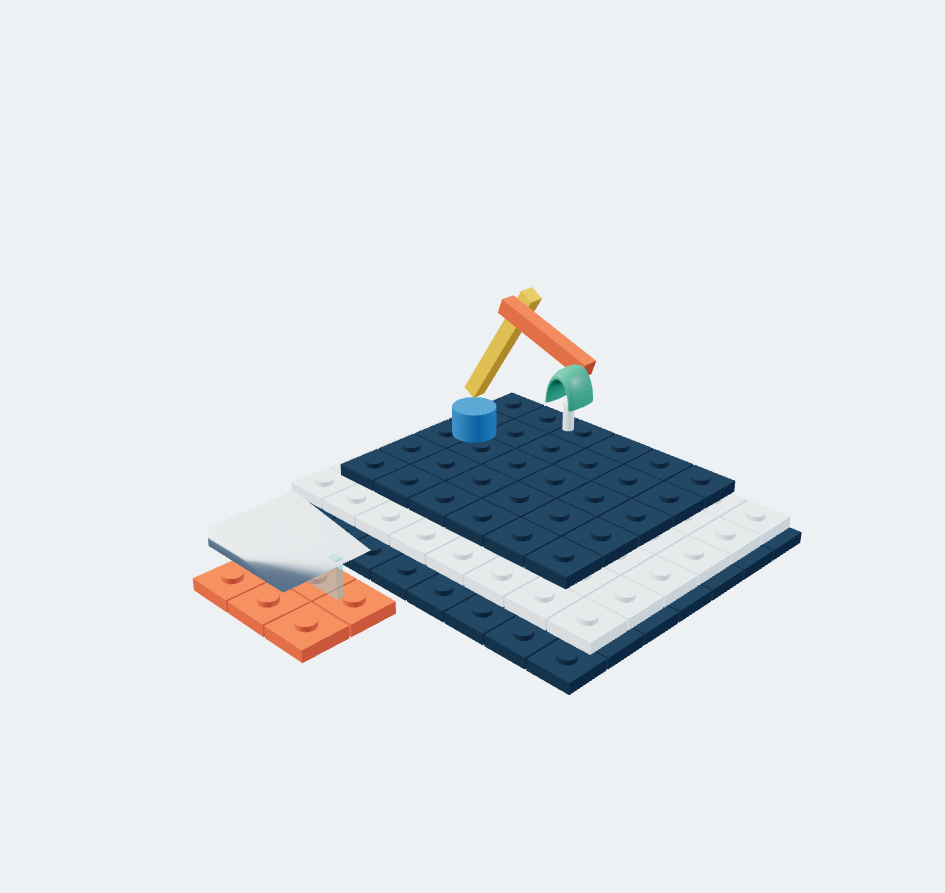
\includegraphics[width=.24\textwidth]{figures/hierarchy-expanded/exp-d2-arm-1-iso.png}
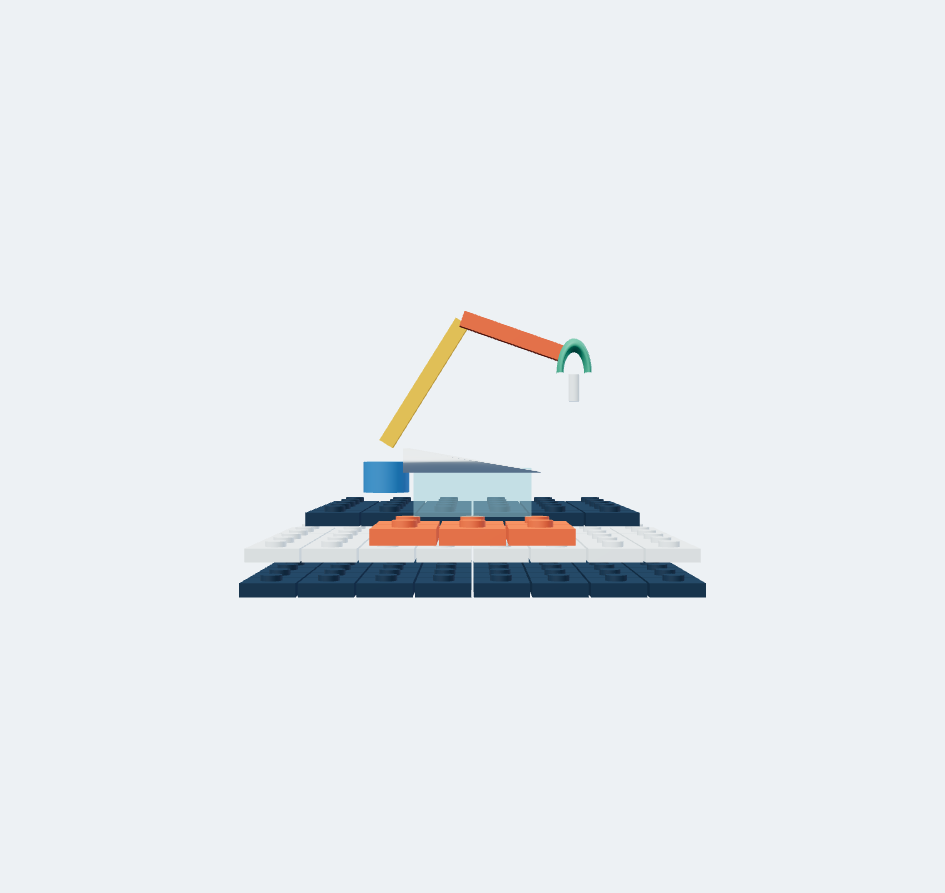
\includegraphics[width=.24\textwidth]{figures/hierarchy-expanded/exp-d2-arm-1-front.png}
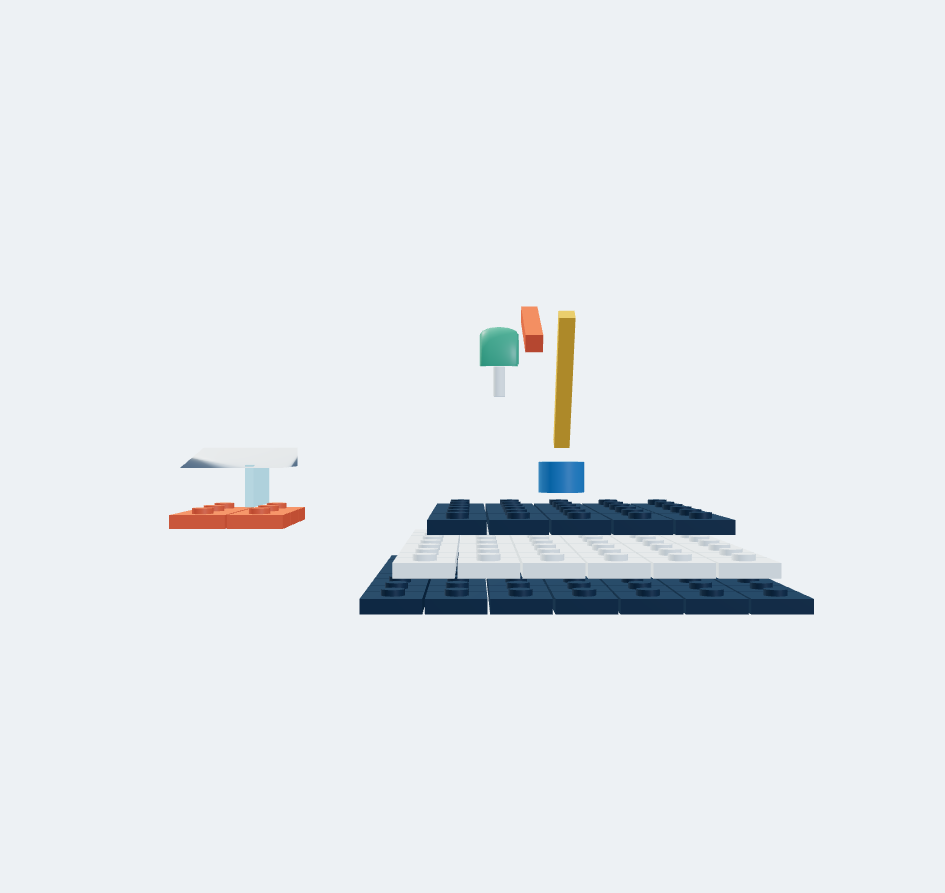
\includegraphics[width=.24\textwidth]{figures/hierarchy-expanded/exp-d2-arm-1-side.png}
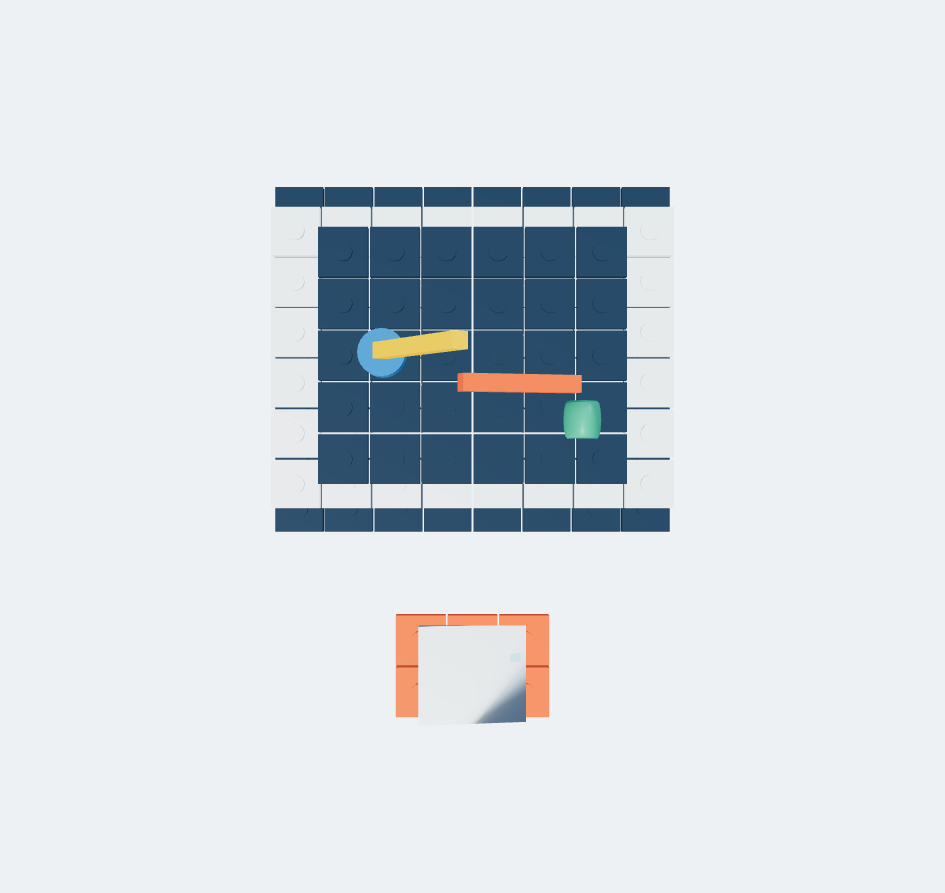
\includegraphics[width=.24\textwidth]{figures/hierarchy-expanded/exp-d2-arm-1-top.png}
\end{center}
\noindent All 48 families share this source. Full inputs and answers appear in the companion question bank.
\begin{center}\tiny\begin{tabular}{rllll}\toprule No. & Family & Layer & Output & Evidence\\\midrule
1 & identify & atomic & single-choice & model-state \\
2 & count & atomic & single-choice & model-state \\
3 & color & atomic & single-choice & model-state \\
4 & position & atomic & single-choice & model-state \\
5 & joint-type & atomic & single-choice & model-state \\
6 & parent & atomic & single-choice & model-state \\
7 & anchor & atomic & single-choice & model-state \\
8 & degree & atomic & single-choice & model-state \\
9 & recolor & atomic & single-choice & model-state \\
10 & add & atomic & single-choice & model-state \\
11 & remove & atomic & single-choice & model-state \\
12 & replace & atomic & single-choice & model-state \\
13 & translate & atomic & single-choice & model-state \\
14 & rotate & atomic & single-choice & model-state \\
15 & next-module & atomic & single-choice & model-state \\
16 & inventory & atomic & single-choice & model-state \\
17 & boundary & atomic & single-choice & model-state \\
18 & no-op & atomic & single-choice & model-state \\
19 & prefix & metacognitive & single-choice & support-graph \\
20 & access & metacognitive & multiple-choice & Rapier \\
21 & counterfactual & metacognitive & single-choice & support-graph \\
22 & dynamic & metacognitive & single-choice & Rapier \\
23 & kinematic & metacognitive & multiple-choice & model-state \\
24 & diagnosis & metacognitive & multiple-choice & model-state \\
25 & information-gain & metacognitive & multiple-choice & finite-world \\
26 & abstention & metacognitive & single-choice & finite-world \\
27 & posterior & metacognitive & single-choice & finite-world \\
28 & pareto & metacognitive & multiple-choice & model-state \\
29 & assembly & procedural & actions & state-machine \\
30 & disassembly & procedural & actions & state-machine \\
31 & service-repair & procedural & actions & state-machine \\
32 & compound-edit & procedural & actions & state-machine \\
33 & multi-fault & integrative & actions & state-machine \\
34 & scheduling & integrative & schedule & resource-schedule \\
35 & policy & integrative & policy & finite-world \\
36 & local-frame & atomic & single-choice & model-state \\
37 & projection & atomic & single-choice & model-state \\
38 & relative-order & atomic & single-choice & model-state \\
39 & joint-axis & atomic & single-choice & model-state \\
40 & clearance-margin & metacognitive & single-choice & model-state \\
41 & load-moment & metacognitive & single-choice & model-state \\
42 & weighted-posterior & metacognitive & single-choice & finite-world \\
43 & expected-loss & metacognitive & single-choice & finite-world \\
44 & trace-threshold & metacognitive & single-choice & Rapier \\
45 & guarded-repair & procedural & actions & state-machine \\
46 & rollback & procedural & actions & state-machine \\
47 & resource-repair & integrative & actions & state-machine \\
48 & budget-policy & integrative & policy & finite-world \\
\bottomrule\end{tabular}\end{center}
\clearpage
\subsection{41. Two-link Sampling Arm Assembly (D2)}
157 visible parts; 8 modules; 7 joints. Representative-point motion 0.0150; rotation 0.0034 rad.
\begin{center}
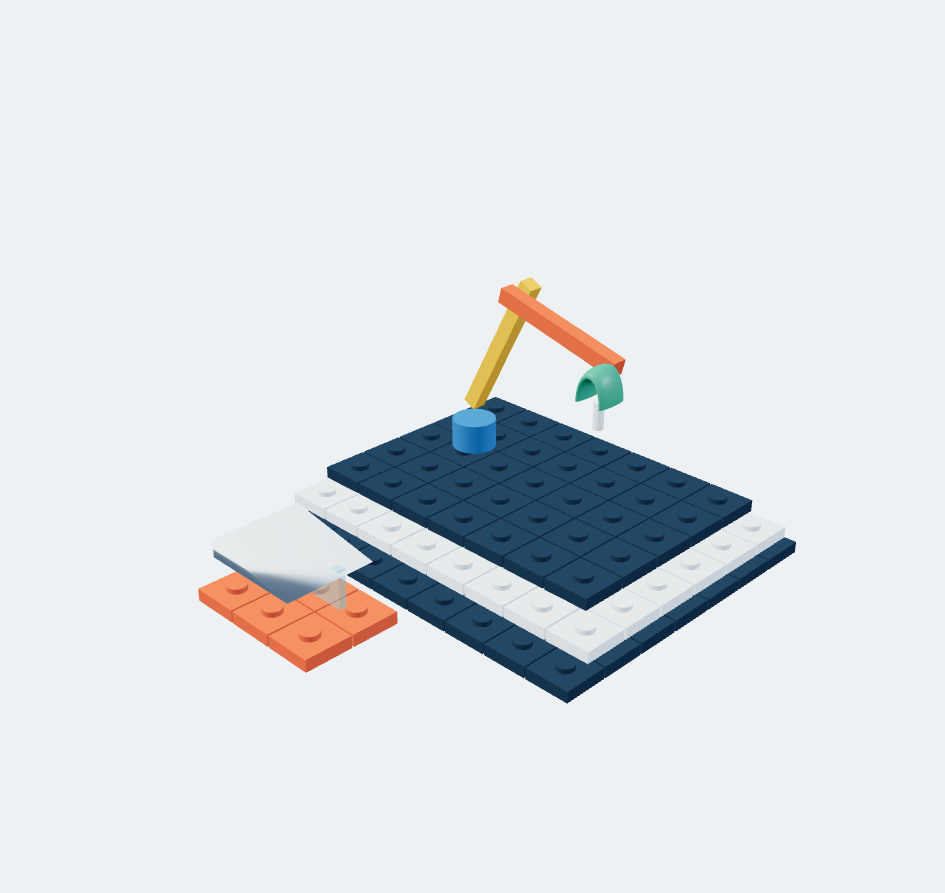
\includegraphics[width=.24\textwidth]{figures/hierarchy-expanded/exp-d2-arm-2-iso.png}
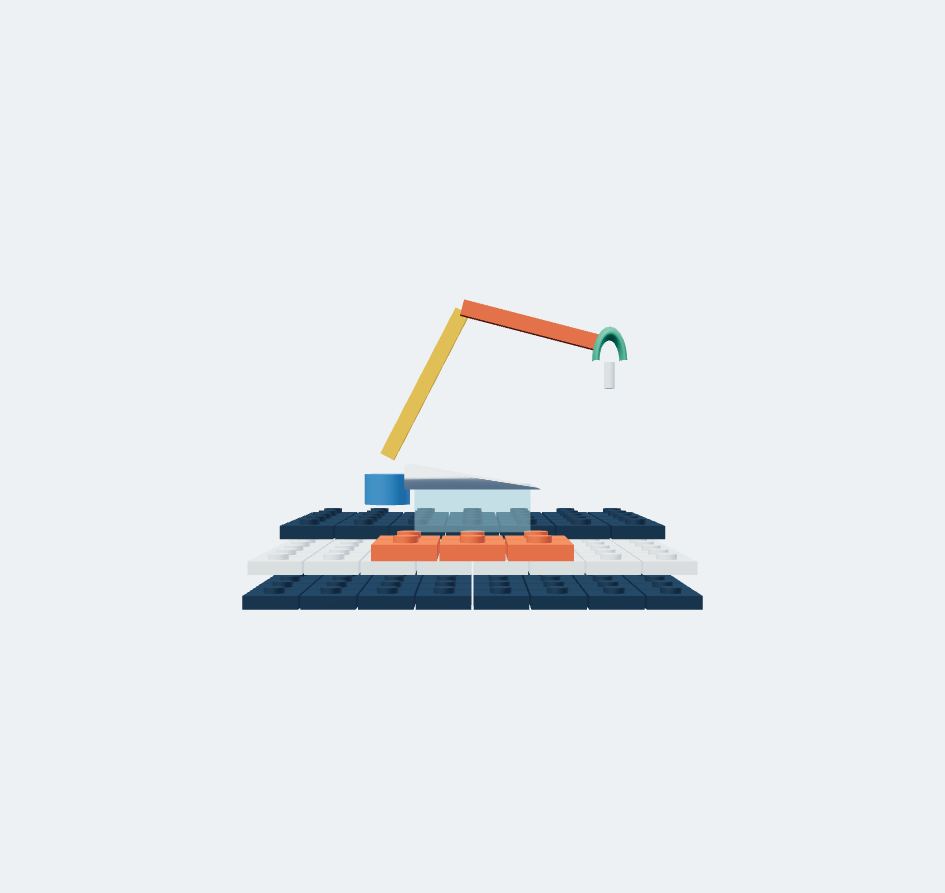
\includegraphics[width=.24\textwidth]{figures/hierarchy-expanded/exp-d2-arm-2-front.png}
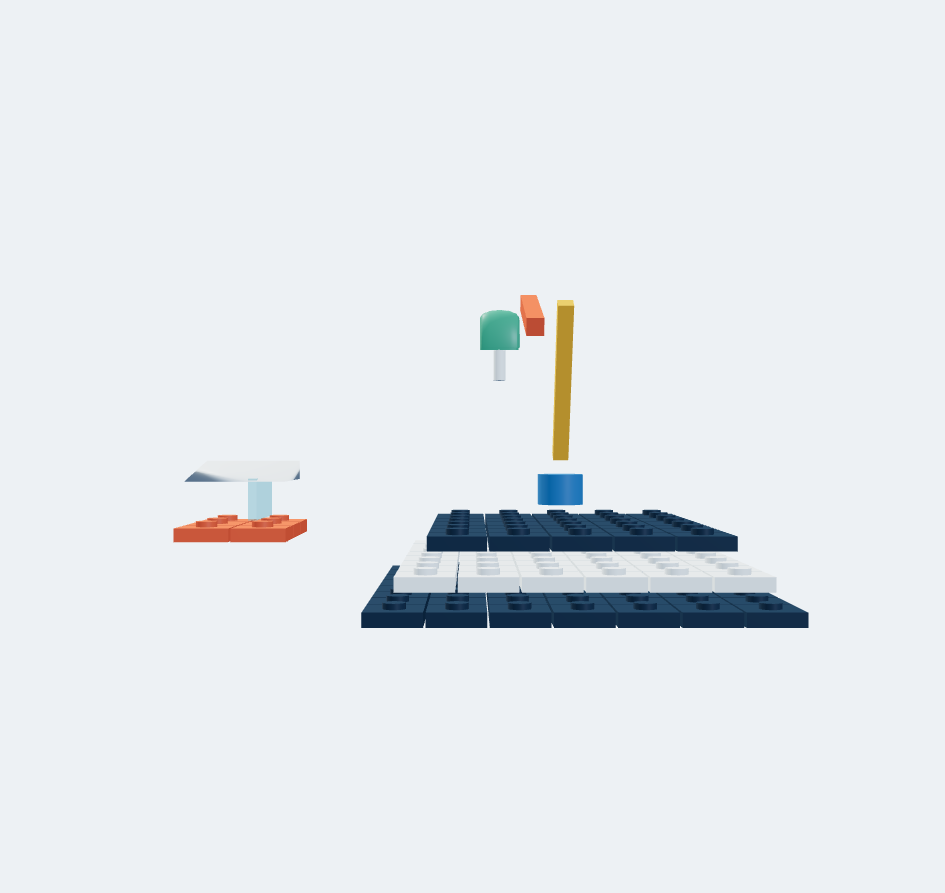
\includegraphics[width=.24\textwidth]{figures/hierarchy-expanded/exp-d2-arm-2-side.png}
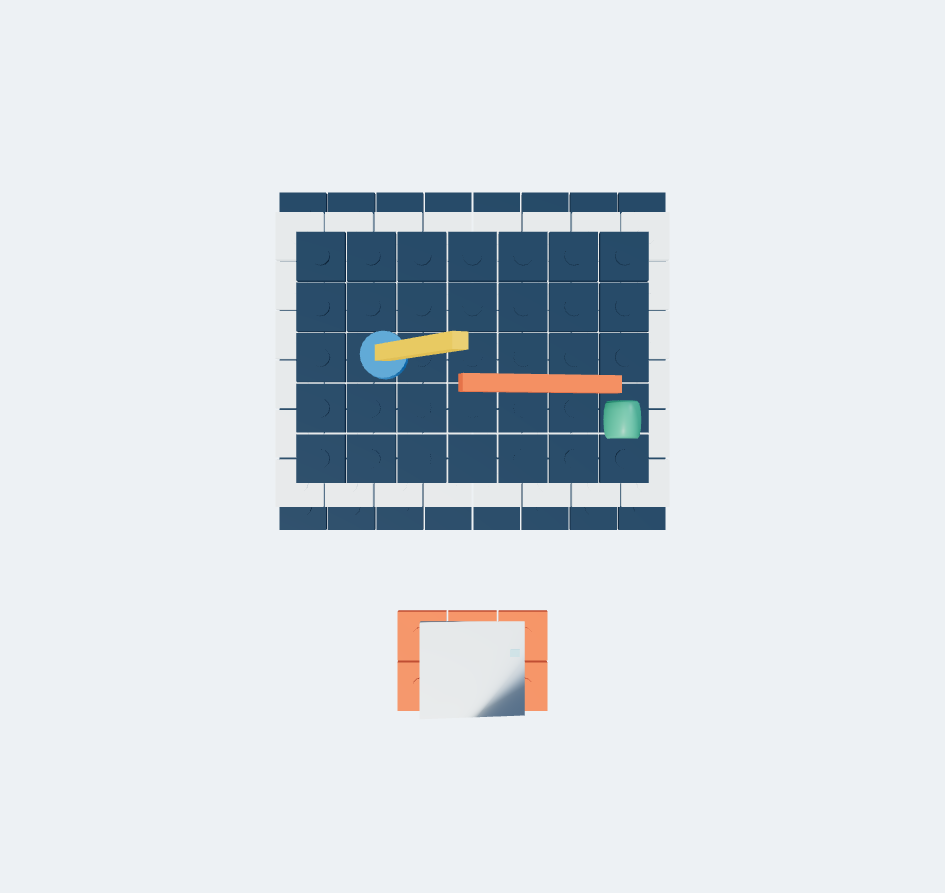
\includegraphics[width=.24\textwidth]{figures/hierarchy-expanded/exp-d2-arm-2-top.png}
\end{center}
\noindent All 48 families share this source. Full inputs and answers appear in the companion question bank.
\begin{center}\tiny\begin{tabular}{rllll}\toprule No. & Family & Layer & Output & Evidence\\\midrule
1 & identify & atomic & single-choice & model-state \\
2 & count & atomic & single-choice & model-state \\
3 & color & atomic & single-choice & model-state \\
4 & position & atomic & single-choice & model-state \\
5 & joint-type & atomic & single-choice & model-state \\
6 & parent & atomic & single-choice & model-state \\
7 & anchor & atomic & single-choice & model-state \\
8 & degree & atomic & single-choice & model-state \\
9 & recolor & atomic & single-choice & model-state \\
10 & add & atomic & single-choice & model-state \\
11 & remove & atomic & single-choice & model-state \\
12 & replace & atomic & single-choice & model-state \\
13 & translate & atomic & single-choice & model-state \\
14 & rotate & atomic & single-choice & model-state \\
15 & next-module & atomic & single-choice & model-state \\
16 & inventory & atomic & single-choice & model-state \\
17 & boundary & atomic & single-choice & model-state \\
18 & no-op & atomic & single-choice & model-state \\
19 & prefix & metacognitive & single-choice & support-graph \\
20 & access & metacognitive & multiple-choice & Rapier \\
21 & counterfactual & metacognitive & single-choice & support-graph \\
22 & dynamic & metacognitive & single-choice & Rapier \\
23 & kinematic & metacognitive & multiple-choice & model-state \\
24 & diagnosis & metacognitive & multiple-choice & model-state \\
25 & information-gain & metacognitive & multiple-choice & finite-world \\
26 & abstention & metacognitive & single-choice & finite-world \\
27 & posterior & metacognitive & single-choice & finite-world \\
28 & pareto & metacognitive & multiple-choice & model-state \\
29 & assembly & procedural & actions & state-machine \\
30 & disassembly & procedural & actions & state-machine \\
31 & service-repair & procedural & actions & state-machine \\
32 & compound-edit & procedural & actions & state-machine \\
33 & multi-fault & integrative & actions & state-machine \\
34 & scheduling & integrative & schedule & resource-schedule \\
35 & policy & integrative & policy & finite-world \\
36 & local-frame & atomic & single-choice & model-state \\
37 & projection & atomic & single-choice & model-state \\
38 & relative-order & atomic & single-choice & model-state \\
39 & joint-axis & atomic & single-choice & model-state \\
40 & clearance-margin & metacognitive & single-choice & model-state \\
41 & load-moment & metacognitive & single-choice & model-state \\
42 & weighted-posterior & metacognitive & single-choice & finite-world \\
43 & expected-loss & metacognitive & single-choice & finite-world \\
44 & trace-threshold & metacognitive & single-choice & Rapier \\
45 & guarded-repair & procedural & actions & state-machine \\
46 & rollback & procedural & actions & state-machine \\
47 & resource-repair & integrative & actions & state-machine \\
48 & budget-policy & integrative & policy & finite-world \\
\bottomrule\end{tabular}\end{center}
\clearpage
\subsection{42. Four-slot Sample Carousel Assembly (D2)}
152 visible parts; 10 modules; 9 joints. Representative-point motion 0.0000; rotation 0.0000 rad.
\begin{center}
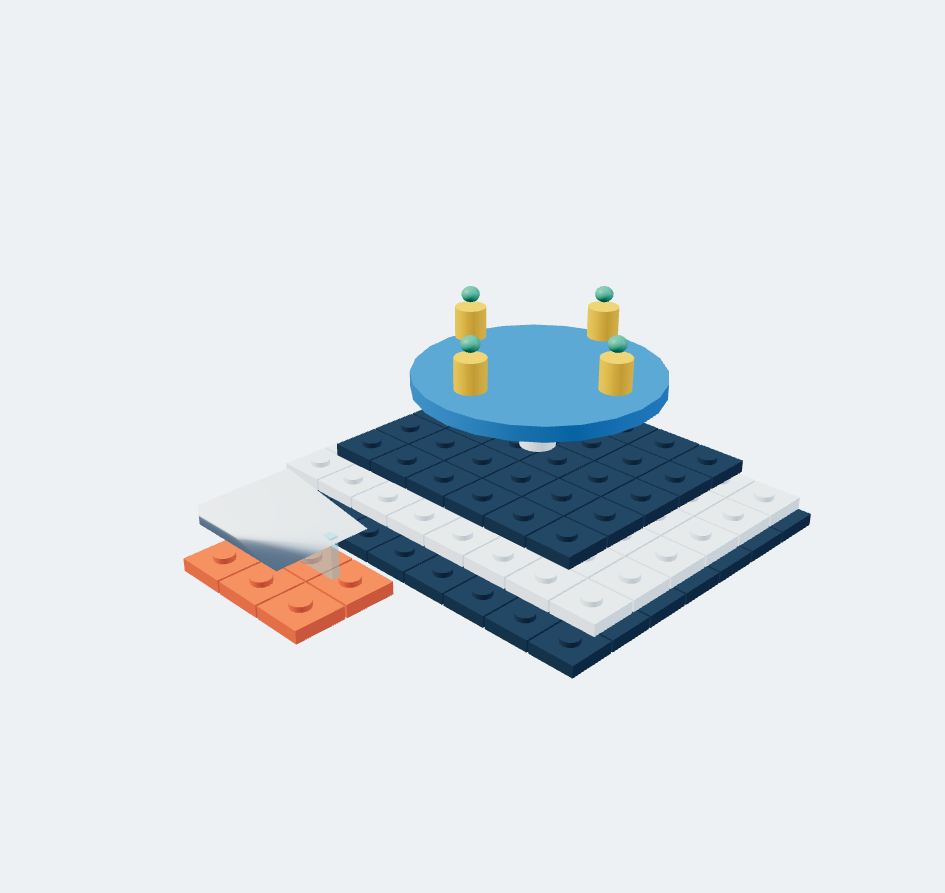
\includegraphics[width=.24\textwidth]{figures/hierarchy-expanded/exp-d2-carousel-1-iso.png}

\includegraphics[width=.24\textwidth]{figures/hierarchy-expanded/exp-d2-carousel-1-front.png}
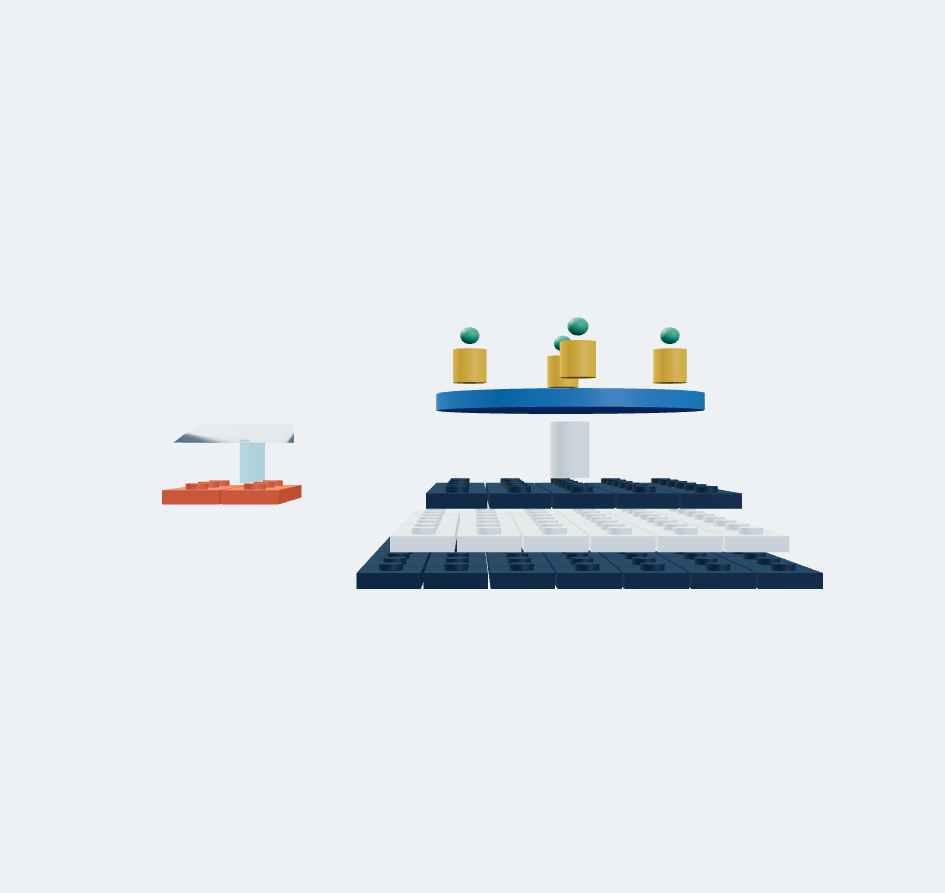
\includegraphics[width=.24\textwidth]{figures/hierarchy-expanded/exp-d2-carousel-1-side.png}
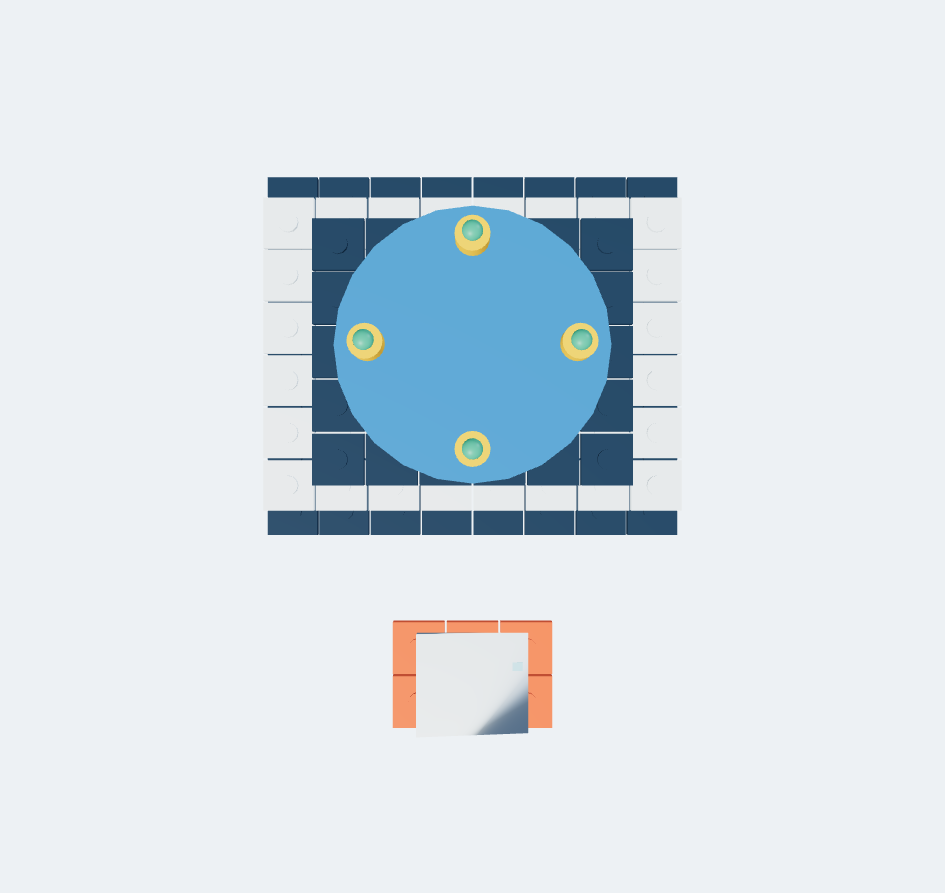
\includegraphics[width=.24\textwidth]{figures/hierarchy-expanded/exp-d2-carousel-1-top.png}
\end{center}
\noindent All 48 families share this source. Full inputs and answers appear in the companion question bank.
\begin{center}\tiny\begin{tabular}{rllll}\toprule No. & Family & Layer & Output & Evidence\\\midrule
1 & identify & atomic & single-choice & model-state \\
2 & count & atomic & single-choice & model-state \\
3 & color & atomic & single-choice & model-state \\
4 & position & atomic & single-choice & model-state \\
5 & joint-type & atomic & single-choice & model-state \\
6 & parent & atomic & single-choice & model-state \\
7 & anchor & atomic & single-choice & model-state \\
8 & degree & atomic & single-choice & model-state \\
9 & recolor & atomic & single-choice & model-state \\
10 & add & atomic & single-choice & model-state \\
11 & remove & atomic & single-choice & model-state \\
12 & replace & atomic & single-choice & model-state \\
13 & translate & atomic & single-choice & model-state \\
14 & rotate & atomic & single-choice & model-state \\
15 & next-module & atomic & single-choice & model-state \\
16 & inventory & atomic & single-choice & model-state \\
17 & boundary & atomic & single-choice & model-state \\
18 & no-op & atomic & single-choice & model-state \\
19 & prefix & metacognitive & single-choice & support-graph \\
20 & access & metacognitive & multiple-choice & Rapier \\
21 & counterfactual & metacognitive & single-choice & support-graph \\
22 & dynamic & metacognitive & single-choice & Rapier \\
23 & kinematic & metacognitive & multiple-choice & model-state \\
24 & diagnosis & metacognitive & multiple-choice & model-state \\
25 & information-gain & metacognitive & multiple-choice & finite-world \\
26 & abstention & metacognitive & single-choice & finite-world \\
27 & posterior & metacognitive & single-choice & finite-world \\
28 & pareto & metacognitive & multiple-choice & model-state \\
29 & assembly & procedural & actions & state-machine \\
30 & disassembly & procedural & actions & state-machine \\
31 & service-repair & procedural & actions & state-machine \\
32 & compound-edit & procedural & actions & state-machine \\
33 & multi-fault & integrative & actions & state-machine \\
34 & scheduling & integrative & schedule & resource-schedule \\
35 & policy & integrative & policy & finite-world \\
36 & local-frame & atomic & single-choice & model-state \\
37 & projection & atomic & single-choice & model-state \\
38 & relative-order & atomic & single-choice & model-state \\
39 & joint-axis & atomic & single-choice & model-state \\
40 & clearance-margin & metacognitive & single-choice & model-state \\
41 & load-moment & metacognitive & single-choice & model-state \\
42 & weighted-posterior & metacognitive & single-choice & finite-world \\
43 & expected-loss & metacognitive & single-choice & finite-world \\
44 & trace-threshold & metacognitive & single-choice & Rapier \\
45 & guarded-repair & procedural & actions & state-machine \\
46 & rollback & procedural & actions & state-machine \\
47 & resource-repair & integrative & actions & state-machine \\
48 & budget-policy & integrative & policy & finite-world \\
\bottomrule\end{tabular}\end{center}
\clearpage
\subsection{43. Six-slot Tube Carousel Assembly (D2)}
161 visible parts; 12 modules; 11 joints. Representative-point motion 0.0000; rotation 0.0000 rad.
\begin{center}
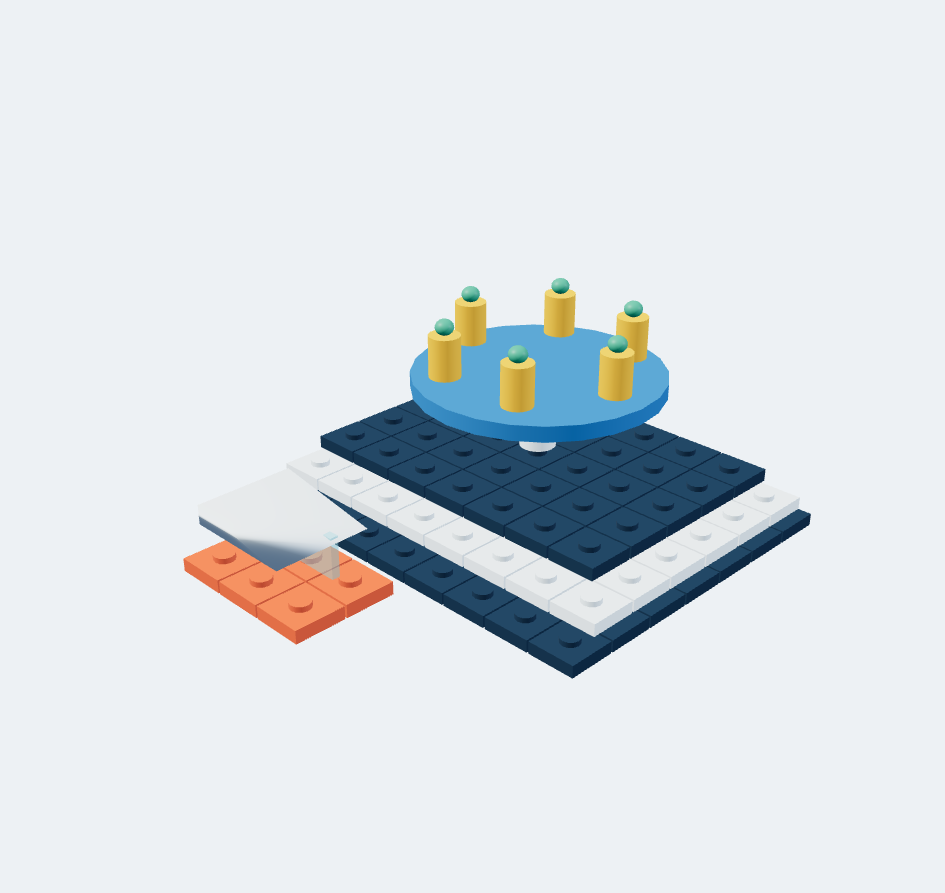
\includegraphics[width=.24\textwidth]{figures/hierarchy-expanded/exp-d2-carousel-2-iso.png}
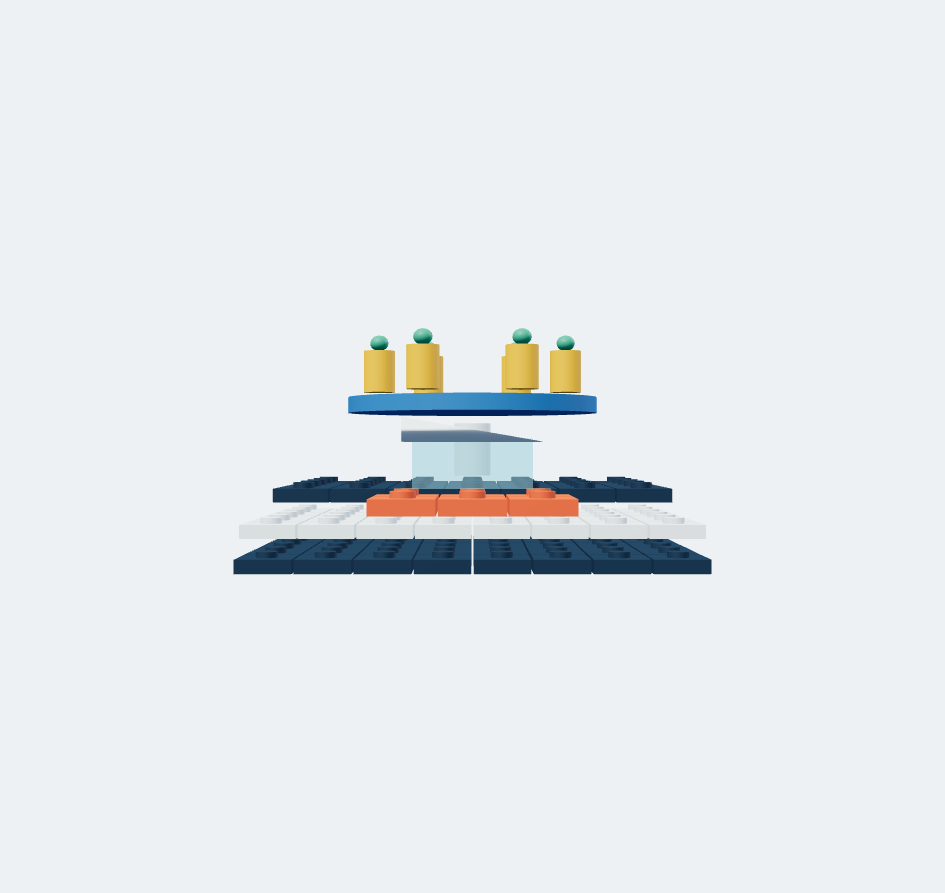
\includegraphics[width=.24\textwidth]{figures/hierarchy-expanded/exp-d2-carousel-2-front.png}
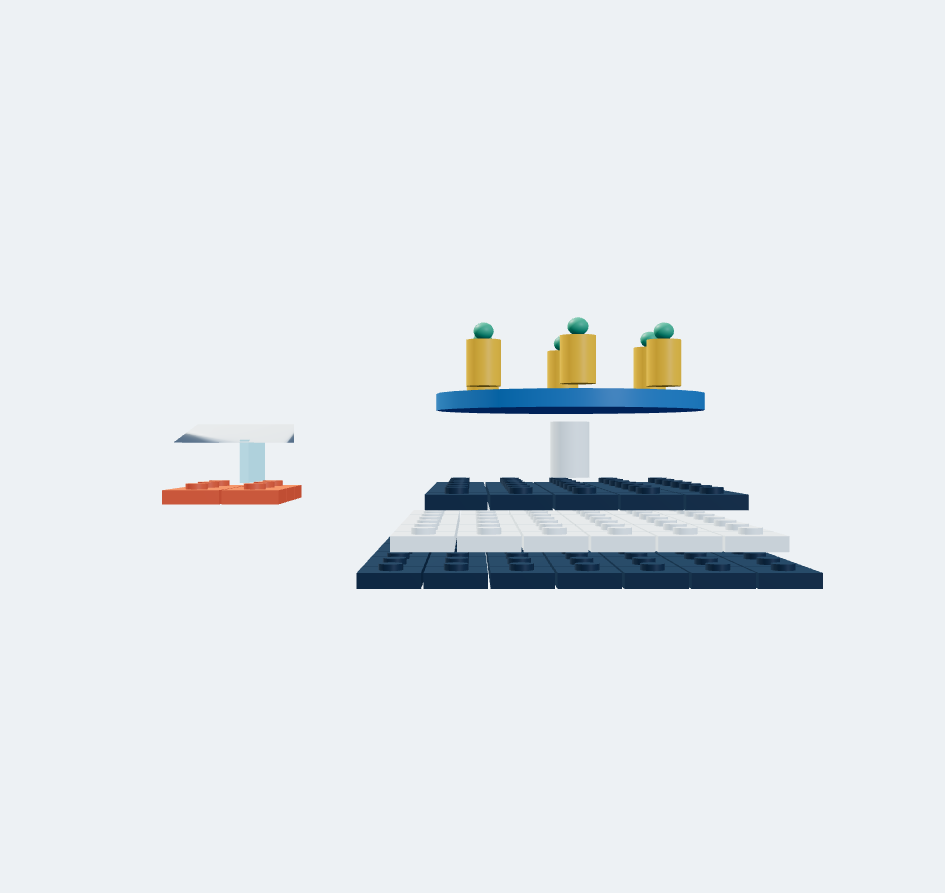
\includegraphics[width=.24\textwidth]{figures/hierarchy-expanded/exp-d2-carousel-2-side.png}
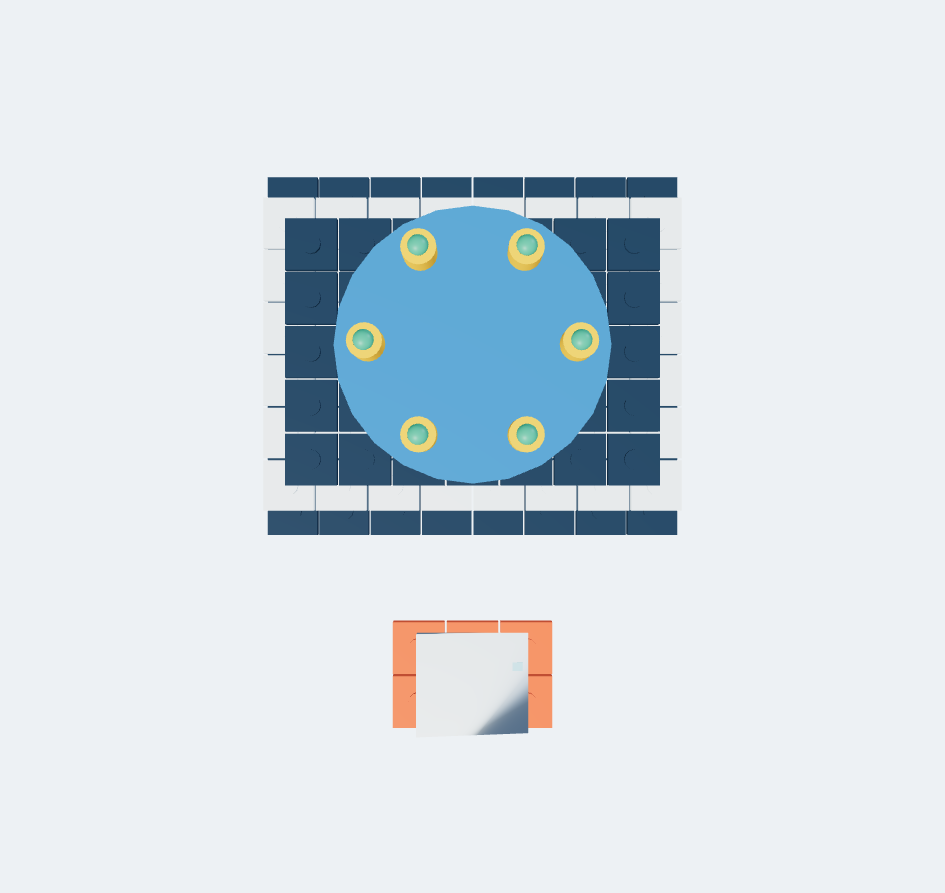
\includegraphics[width=.24\textwidth]{figures/hierarchy-expanded/exp-d2-carousel-2-top.png}
\end{center}
\noindent All 48 families share this source. Full inputs and answers appear in the companion question bank.
\begin{center}\tiny\begin{tabular}{rllll}\toprule No. & Family & Layer & Output & Evidence\\\midrule
1 & identify & atomic & single-choice & model-state \\
2 & count & atomic & single-choice & model-state \\
3 & color & atomic & single-choice & model-state \\
4 & position & atomic & single-choice & model-state \\
5 & joint-type & atomic & single-choice & model-state \\
6 & parent & atomic & single-choice & model-state \\
7 & anchor & atomic & single-choice & model-state \\
8 & degree & atomic & single-choice & model-state \\
9 & recolor & atomic & single-choice & model-state \\
10 & add & atomic & single-choice & model-state \\
11 & remove & atomic & single-choice & model-state \\
12 & replace & atomic & single-choice & model-state \\
13 & translate & atomic & single-choice & model-state \\
14 & rotate & atomic & single-choice & model-state \\
15 & next-module & atomic & single-choice & model-state \\
16 & inventory & atomic & single-choice & model-state \\
17 & boundary & atomic & single-choice & model-state \\
18 & no-op & atomic & single-choice & model-state \\
19 & prefix & metacognitive & single-choice & support-graph \\
20 & access & metacognitive & multiple-choice & Rapier \\
21 & counterfactual & metacognitive & single-choice & support-graph \\
22 & dynamic & metacognitive & single-choice & Rapier \\
23 & kinematic & metacognitive & multiple-choice & model-state \\
24 & diagnosis & metacognitive & multiple-choice & model-state \\
25 & information-gain & metacognitive & multiple-choice & finite-world \\
26 & abstention & metacognitive & single-choice & finite-world \\
27 & posterior & metacognitive & single-choice & finite-world \\
28 & pareto & metacognitive & multiple-choice & model-state \\
29 & assembly & procedural & actions & state-machine \\
30 & disassembly & procedural & actions & state-machine \\
31 & service-repair & procedural & actions & state-machine \\
32 & compound-edit & procedural & actions & state-machine \\
33 & multi-fault & integrative & actions & state-machine \\
34 & scheduling & integrative & schedule & resource-schedule \\
35 & policy & integrative & policy & finite-world \\
36 & local-frame & atomic & single-choice & model-state \\
37 & projection & atomic & single-choice & model-state \\
38 & relative-order & atomic & single-choice & model-state \\
39 & joint-axis & atomic & single-choice & model-state \\
40 & clearance-margin & metacognitive & single-choice & model-state \\
41 & load-moment & metacognitive & single-choice & model-state \\
42 & weighted-posterior & metacognitive & single-choice & finite-world \\
43 & expected-loss & metacognitive & single-choice & finite-world \\
44 & trace-threshold & metacognitive & single-choice & Rapier \\
45 & guarded-repair & procedural & actions & state-machine \\
46 & rollback & procedural & actions & state-machine \\
47 & resource-repair & integrative & actions & state-machine \\
48 & budget-policy & integrative & policy & finite-world \\
\bottomrule\end{tabular}\end{center}
\clearpage
\subsection{44. Tilting Cradle Assembly (D2)}
156 visible parts; 7 modules; 6 joints. Representative-point motion 0.0000; rotation 0.0000 rad.
\begin{center}
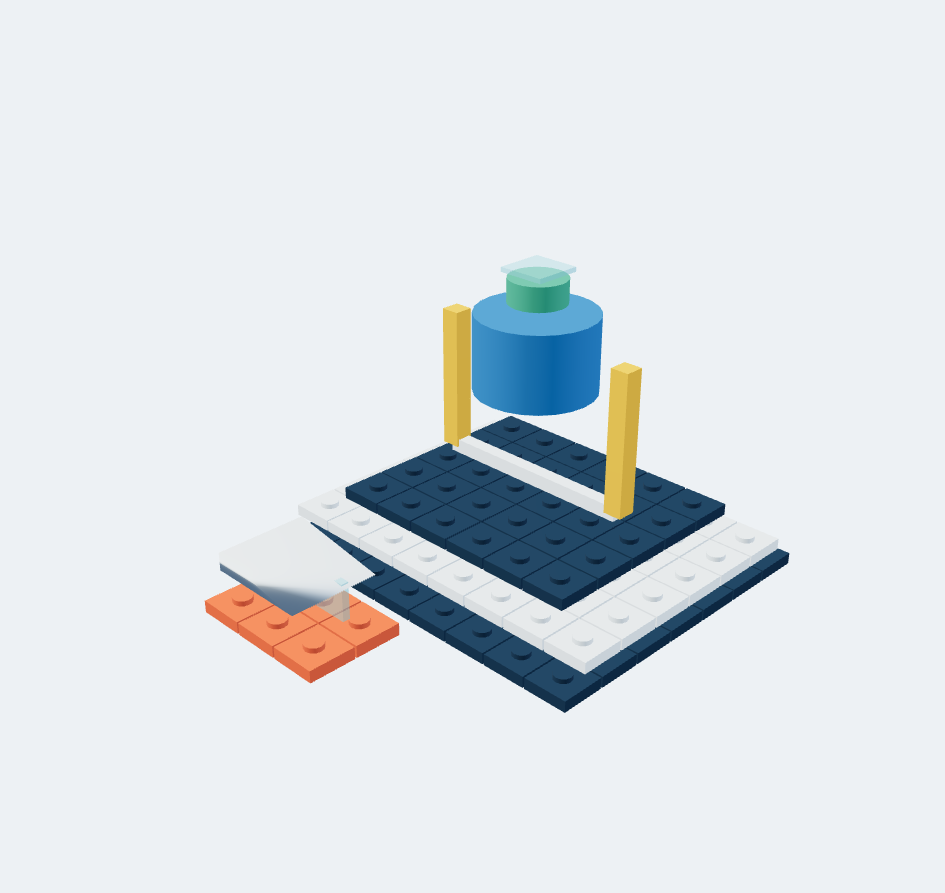
\includegraphics[width=.24\textwidth]{figures/hierarchy-expanded/exp-d2-cradle-1-iso.png}
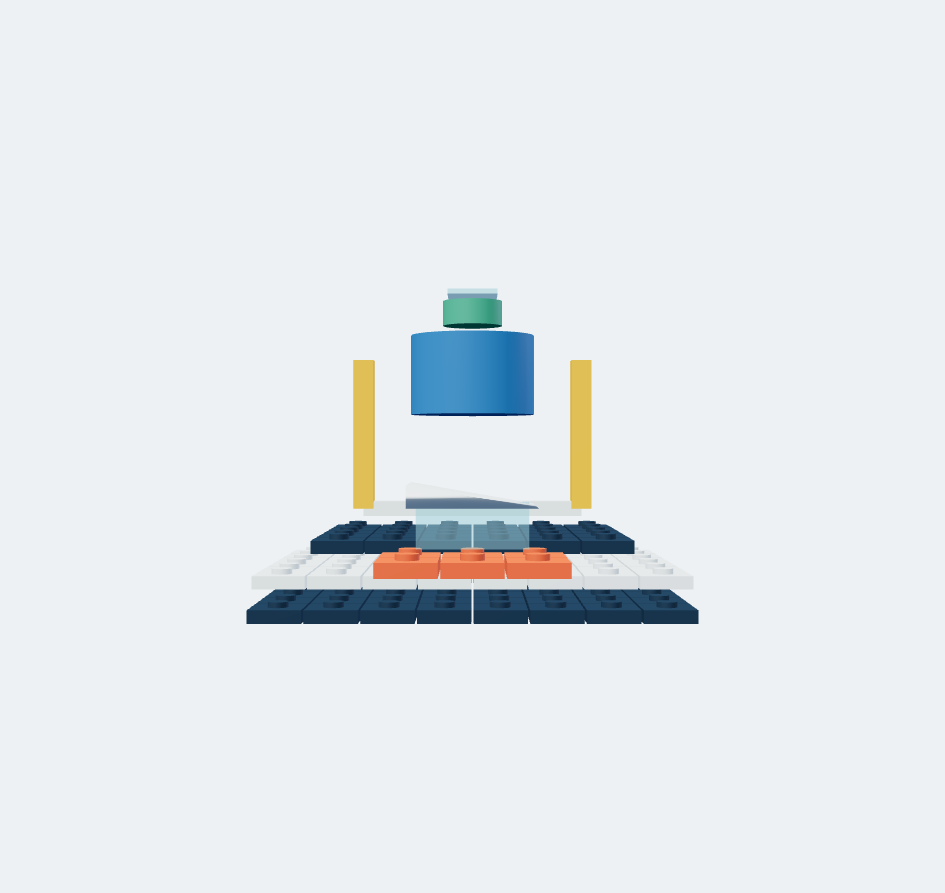
\includegraphics[width=.24\textwidth]{figures/hierarchy-expanded/exp-d2-cradle-1-front.png}
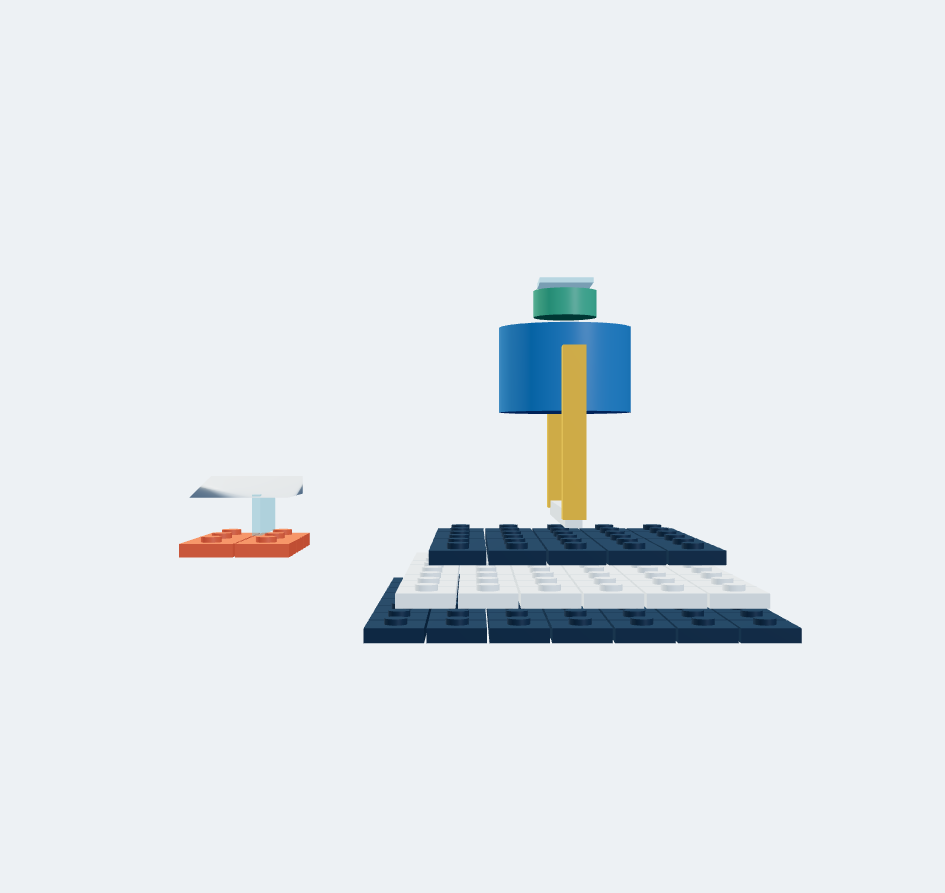
\includegraphics[width=.24\textwidth]{figures/hierarchy-expanded/exp-d2-cradle-1-side.png}
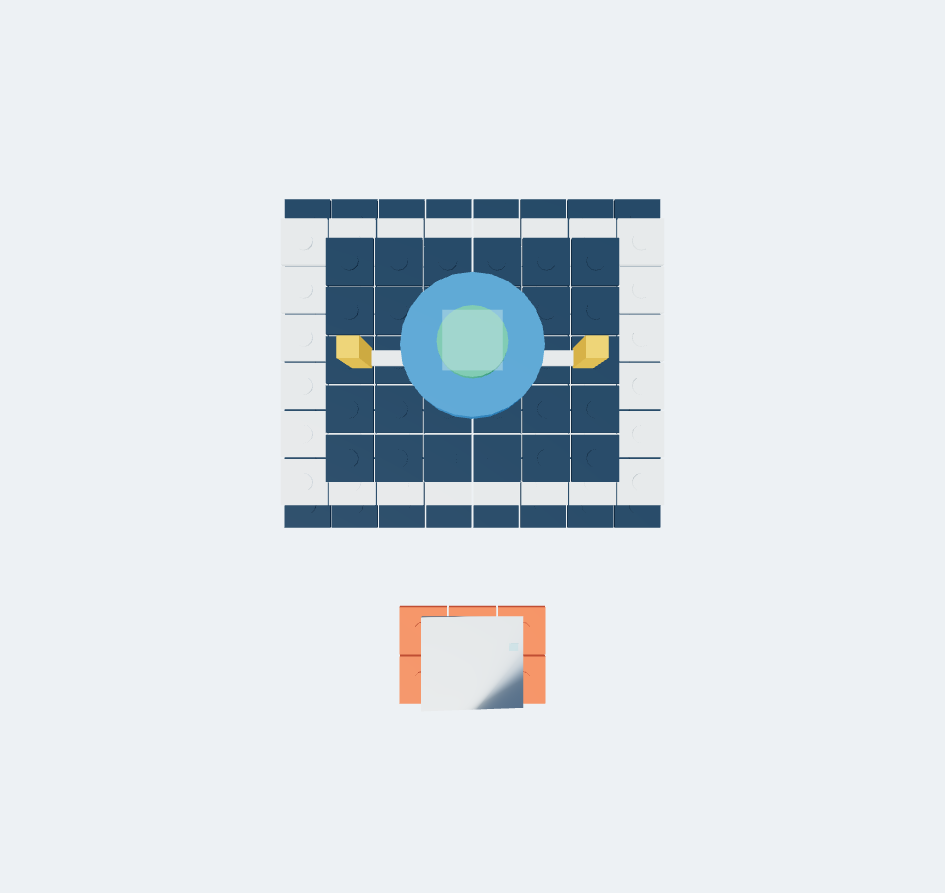
\includegraphics[width=.24\textwidth]{figures/hierarchy-expanded/exp-d2-cradle-1-top.png}
\end{center}
\noindent All 48 families share this source. Full inputs and answers appear in the companion question bank.
\begin{center}\tiny\begin{tabular}{rllll}\toprule No. & Family & Layer & Output & Evidence\\\midrule
1 & identify & atomic & single-choice & model-state \\
2 & count & atomic & single-choice & model-state \\
3 & color & atomic & single-choice & model-state \\
4 & position & atomic & single-choice & model-state \\
5 & joint-type & atomic & single-choice & model-state \\
6 & parent & atomic & single-choice & model-state \\
7 & anchor & atomic & single-choice & model-state \\
8 & degree & atomic & single-choice & model-state \\
9 & recolor & atomic & single-choice & model-state \\
10 & add & atomic & single-choice & model-state \\
11 & remove & atomic & single-choice & model-state \\
12 & replace & atomic & single-choice & model-state \\
13 & translate & atomic & single-choice & model-state \\
14 & rotate & atomic & single-choice & model-state \\
15 & next-module & atomic & single-choice & model-state \\
16 & inventory & atomic & single-choice & model-state \\
17 & boundary & atomic & single-choice & model-state \\
18 & no-op & atomic & single-choice & model-state \\
19 & prefix & metacognitive & single-choice & support-graph \\
20 & access & metacognitive & multiple-choice & Rapier \\
21 & counterfactual & metacognitive & single-choice & support-graph \\
22 & dynamic & metacognitive & single-choice & Rapier \\
23 & kinematic & metacognitive & multiple-choice & model-state \\
24 & diagnosis & metacognitive & multiple-choice & model-state \\
25 & information-gain & metacognitive & multiple-choice & finite-world \\
26 & abstention & metacognitive & single-choice & finite-world \\
27 & posterior & metacognitive & single-choice & finite-world \\
28 & pareto & metacognitive & multiple-choice & model-state \\
29 & assembly & procedural & actions & state-machine \\
30 & disassembly & procedural & actions & state-machine \\
31 & service-repair & procedural & actions & state-machine \\
32 & compound-edit & procedural & actions & state-machine \\
33 & multi-fault & integrative & actions & state-machine \\
34 & scheduling & integrative & schedule & resource-schedule \\
35 & policy & integrative & policy & finite-world \\
36 & local-frame & atomic & single-choice & model-state \\
37 & projection & atomic & single-choice & model-state \\
38 & relative-order & atomic & single-choice & model-state \\
39 & joint-axis & atomic & single-choice & model-state \\
40 & clearance-margin & metacognitive & single-choice & model-state \\
41 & load-moment & metacognitive & single-choice & model-state \\
42 & weighted-posterior & metacognitive & single-choice & finite-world \\
43 & expected-loss & metacognitive & single-choice & finite-world \\
44 & trace-threshold & metacognitive & single-choice & Rapier \\
45 & guarded-repair & procedural & actions & state-machine \\
46 & rollback & procedural & actions & state-machine \\
47 & resource-repair & integrative & actions & state-machine \\
48 & budget-policy & integrative & policy & finite-world \\
\bottomrule\end{tabular}\end{center}
\clearpage
\subsection{45. Two-axis Optical Cradle Assembly (D2)}
161 visible parts; 7 modules; 6 joints. Representative-point motion 0.0000; rotation 0.0000 rad.
\begin{center}
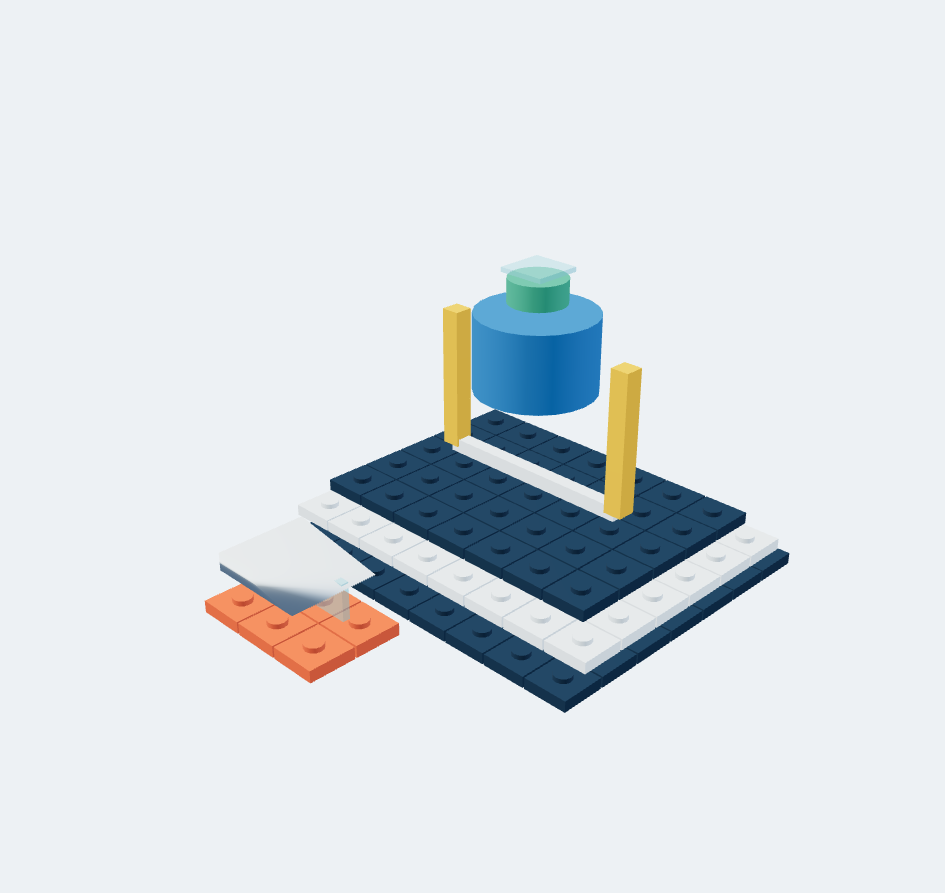
\includegraphics[width=.24\textwidth]{figures/hierarchy-expanded/exp-d2-cradle-2-iso.png}
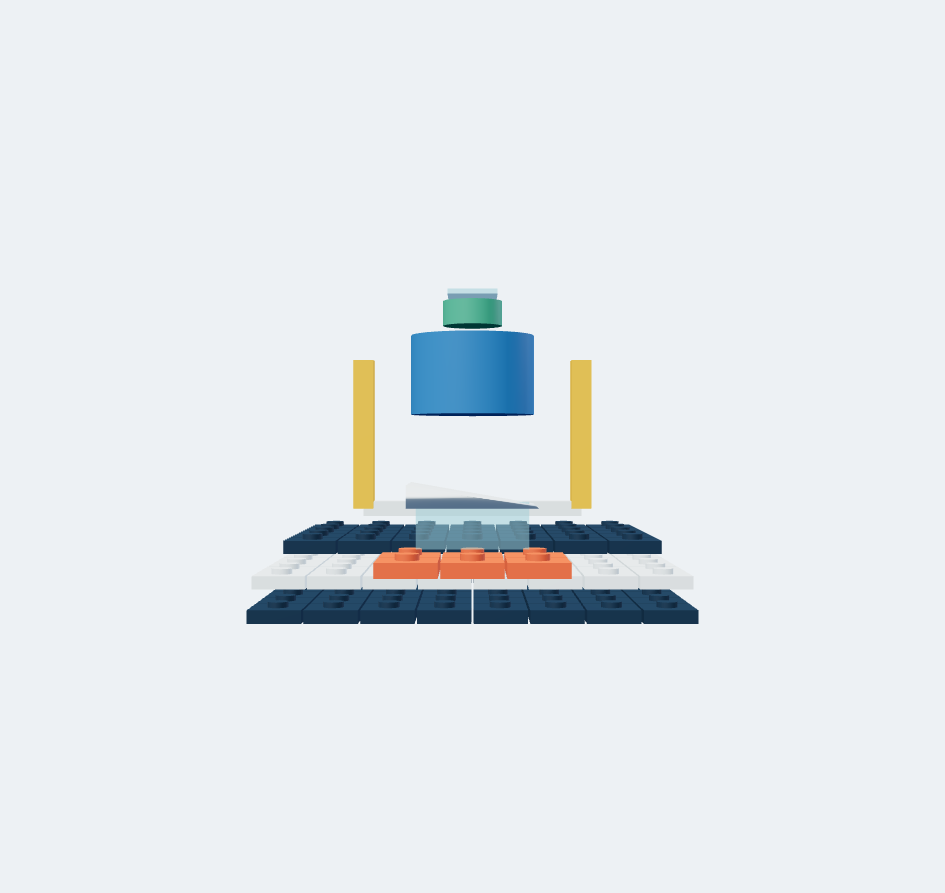
\includegraphics[width=.24\textwidth]{figures/hierarchy-expanded/exp-d2-cradle-2-front.png}
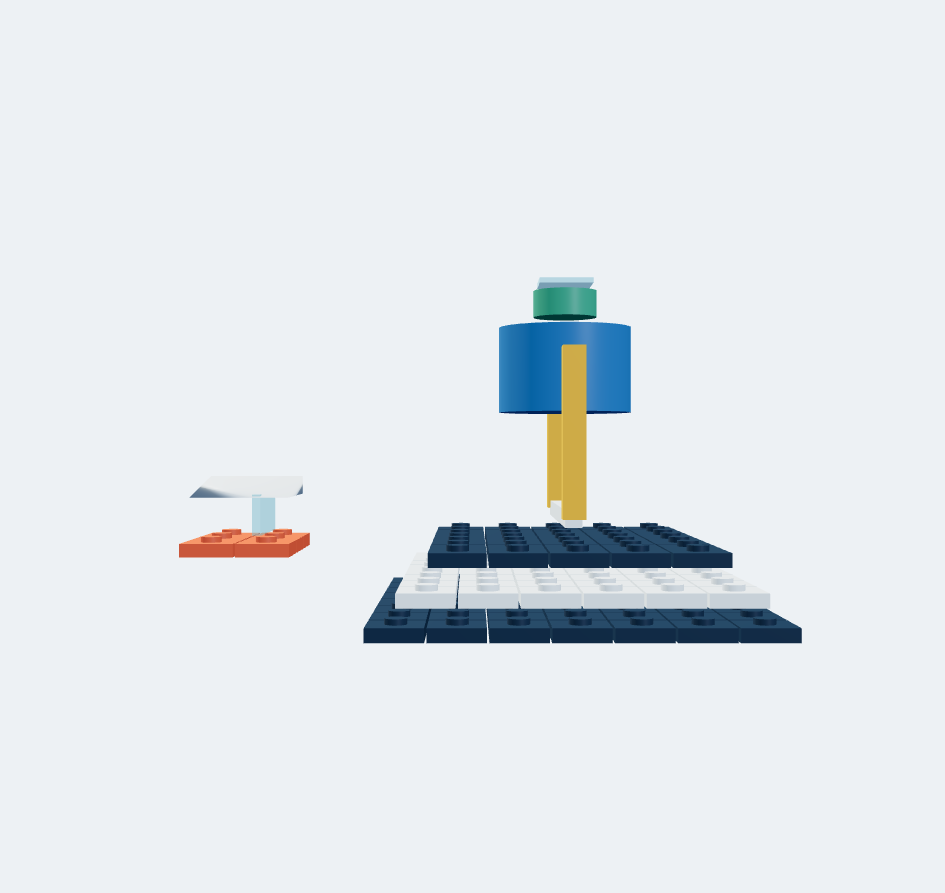
\includegraphics[width=.24\textwidth]{figures/hierarchy-expanded/exp-d2-cradle-2-side.png}
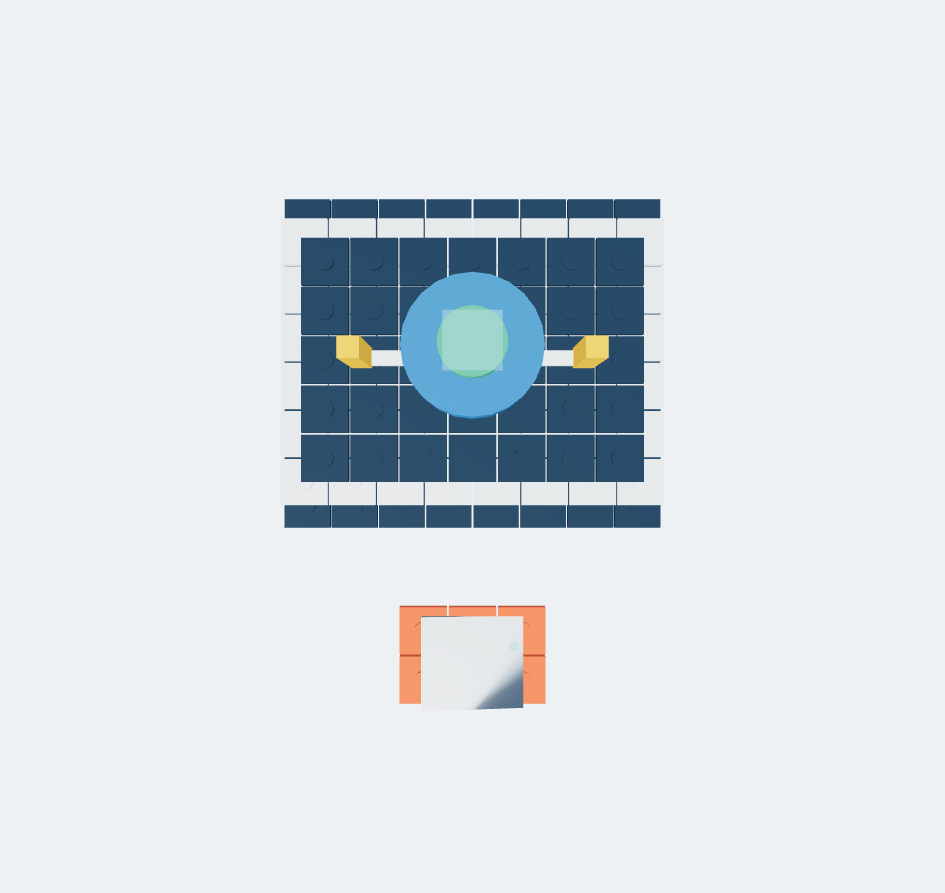
\includegraphics[width=.24\textwidth]{figures/hierarchy-expanded/exp-d2-cradle-2-top.png}
\end{center}
\noindent All 48 families share this source. Full inputs and answers appear in the companion question bank.
\begin{center}\tiny\begin{tabular}{rllll}\toprule No. & Family & Layer & Output & Evidence\\\midrule
1 & identify & atomic & single-choice & model-state \\
2 & count & atomic & single-choice & model-state \\
3 & color & atomic & single-choice & model-state \\
4 & position & atomic & single-choice & model-state \\
5 & joint-type & atomic & single-choice & model-state \\
6 & parent & atomic & single-choice & model-state \\
7 & anchor & atomic & single-choice & model-state \\
8 & degree & atomic & single-choice & model-state \\
9 & recolor & atomic & single-choice & model-state \\
10 & add & atomic & single-choice & model-state \\
11 & remove & atomic & single-choice & model-state \\
12 & replace & atomic & single-choice & model-state \\
13 & translate & atomic & single-choice & model-state \\
14 & rotate & atomic & single-choice & model-state \\
15 & next-module & atomic & single-choice & model-state \\
16 & inventory & atomic & single-choice & model-state \\
17 & boundary & atomic & single-choice & model-state \\
18 & no-op & atomic & single-choice & model-state \\
19 & prefix & metacognitive & single-choice & support-graph \\
20 & access & metacognitive & multiple-choice & Rapier \\
21 & counterfactual & metacognitive & single-choice & support-graph \\
22 & dynamic & metacognitive & single-choice & Rapier \\
23 & kinematic & metacognitive & multiple-choice & model-state \\
24 & diagnosis & metacognitive & multiple-choice & model-state \\
25 & information-gain & metacognitive & multiple-choice & finite-world \\
26 & abstention & metacognitive & single-choice & finite-world \\
27 & posterior & metacognitive & single-choice & finite-world \\
28 & pareto & metacognitive & multiple-choice & model-state \\
29 & assembly & procedural & actions & state-machine \\
30 & disassembly & procedural & actions & state-machine \\
31 & service-repair & procedural & actions & state-machine \\
32 & compound-edit & procedural & actions & state-machine \\
33 & multi-fault & integrative & actions & state-machine \\
34 & scheduling & integrative & schedule & resource-schedule \\
35 & policy & integrative & policy & finite-world \\
36 & local-frame & atomic & single-choice & model-state \\
37 & projection & atomic & single-choice & model-state \\
38 & relative-order & atomic & single-choice & model-state \\
39 & joint-axis & atomic & single-choice & model-state \\
40 & clearance-margin & metacognitive & single-choice & model-state \\
41 & load-moment & metacognitive & single-choice & model-state \\
42 & weighted-posterior & metacognitive & single-choice & finite-world \\
43 & expected-loss & metacognitive & single-choice & finite-world \\
44 & trace-threshold & metacognitive & single-choice & Rapier \\
45 & guarded-repair & procedural & actions & state-machine \\
46 & rollback & procedural & actions & state-machine \\
47 & resource-repair & integrative & actions & state-machine \\
48 & budget-policy & integrative & policy & finite-world \\
\bottomrule\end{tabular}\end{center}
\clearpage
\subsection{46. Horizontal Drum Stand Assembly (D2)}
151 visible parts; 5 modules; 4 joints. Representative-point motion 0.0000; rotation 0.0000 rad.
\begin{center}
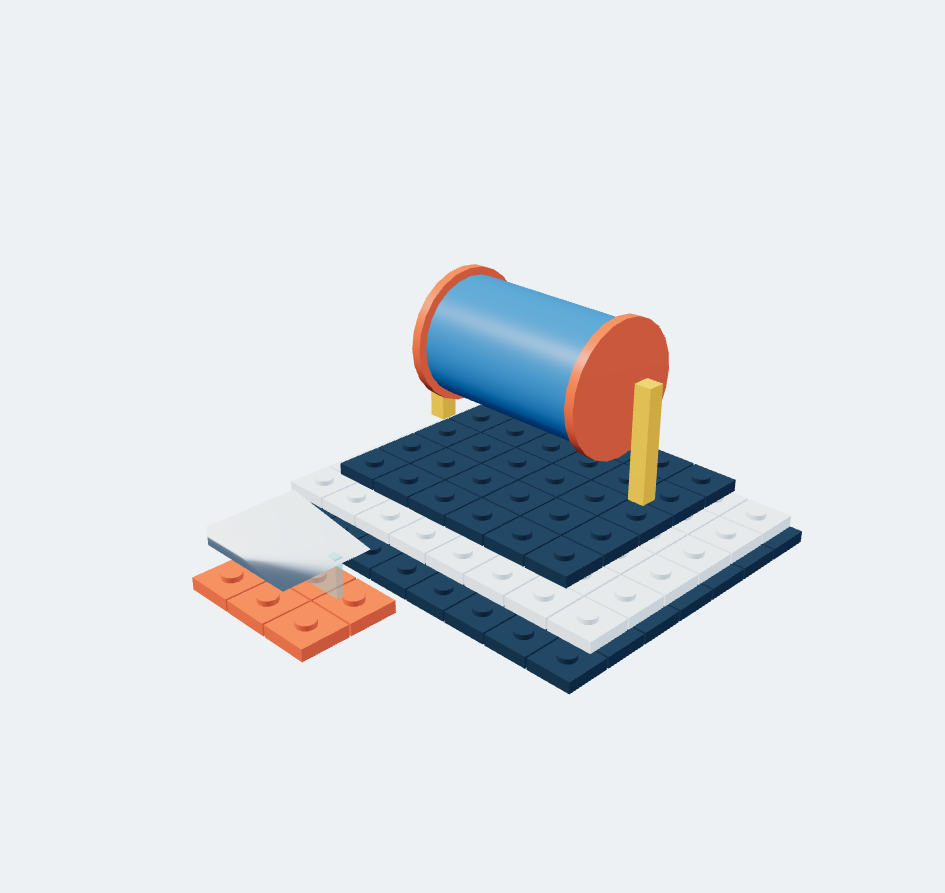
\includegraphics[width=.24\textwidth]{figures/hierarchy-expanded/exp-d2-drum-1-iso.png}

\includegraphics[width=.24\textwidth]{figures/hierarchy-expanded/exp-d2-drum-1-front.png}

\includegraphics[width=.24\textwidth]{figures/hierarchy-expanded/exp-d2-drum-1-side.png}
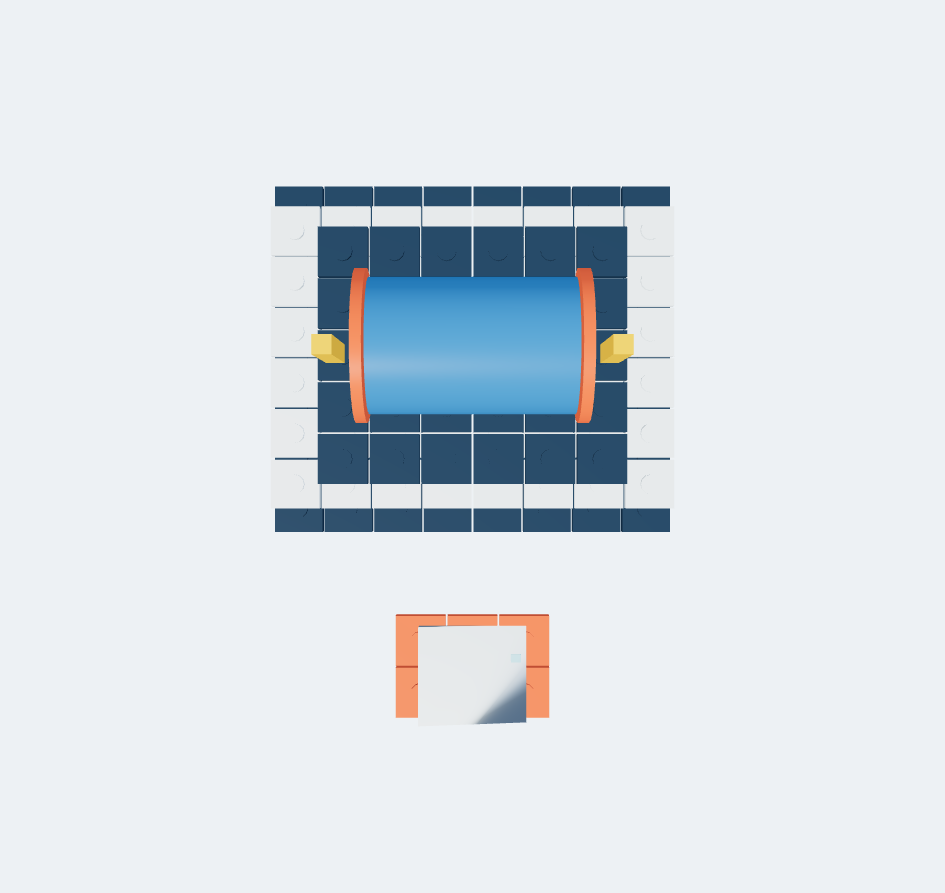
\includegraphics[width=.24\textwidth]{figures/hierarchy-expanded/exp-d2-drum-1-top.png}
\end{center}
\noindent All 48 families share this source. Full inputs and answers appear in the companion question bank.
\begin{center}\tiny\begin{tabular}{rllll}\toprule No. & Family & Layer & Output & Evidence\\\midrule
1 & identify & atomic & single-choice & model-state \\
2 & count & atomic & single-choice & model-state \\
3 & color & atomic & single-choice & model-state \\
4 & position & atomic & single-choice & model-state \\
5 & joint-type & atomic & single-choice & model-state \\
6 & parent & atomic & single-choice & model-state \\
7 & anchor & atomic & single-choice & model-state \\
8 & degree & atomic & single-choice & model-state \\
9 & recolor & atomic & single-choice & model-state \\
10 & add & atomic & single-choice & model-state \\
11 & remove & atomic & single-choice & model-state \\
12 & replace & atomic & single-choice & model-state \\
13 & translate & atomic & single-choice & model-state \\
14 & rotate & atomic & single-choice & model-state \\
15 & next-module & atomic & single-choice & model-state \\
16 & inventory & atomic & single-choice & model-state \\
17 & boundary & atomic & single-choice & model-state \\
18 & no-op & atomic & single-choice & model-state \\
19 & prefix & metacognitive & single-choice & support-graph \\
20 & access & metacognitive & multiple-choice & Rapier \\
21 & counterfactual & metacognitive & single-choice & support-graph \\
22 & dynamic & metacognitive & single-choice & Rapier \\
23 & kinematic & metacognitive & multiple-choice & model-state \\
24 & diagnosis & metacognitive & multiple-choice & model-state \\
25 & information-gain & metacognitive & multiple-choice & finite-world \\
26 & abstention & metacognitive & single-choice & finite-world \\
27 & posterior & metacognitive & single-choice & finite-world \\
28 & pareto & metacognitive & multiple-choice & model-state \\
29 & assembly & procedural & actions & state-machine \\
30 & disassembly & procedural & actions & state-machine \\
31 & service-repair & procedural & actions & state-machine \\
32 & compound-edit & procedural & actions & state-machine \\
33 & multi-fault & integrative & actions & state-machine \\
34 & scheduling & integrative & schedule & resource-schedule \\
35 & policy & integrative & policy & finite-world \\
36 & local-frame & atomic & single-choice & model-state \\
37 & projection & atomic & single-choice & model-state \\
38 & relative-order & atomic & single-choice & model-state \\
39 & joint-axis & atomic & single-choice & model-state \\
40 & clearance-margin & metacognitive & single-choice & model-state \\
41 & load-moment & metacognitive & single-choice & model-state \\
42 & weighted-posterior & metacognitive & single-choice & finite-world \\
43 & expected-loss & metacognitive & single-choice & finite-world \\
44 & trace-threshold & metacognitive & single-choice & Rapier \\
45 & guarded-repair & procedural & actions & state-machine \\
46 & rollback & procedural & actions & state-machine \\
47 & resource-repair & integrative & actions & state-machine \\
48 & budget-policy & integrative & policy & finite-world \\
\bottomrule\end{tabular}\end{center}
\clearpage
\subsection{47. Twin-drum Indexer Assembly (D2)}
159 visible parts; 6 modules; 5 joints. Representative-point motion 0.0000; rotation 0.0000 rad.
\begin{center}
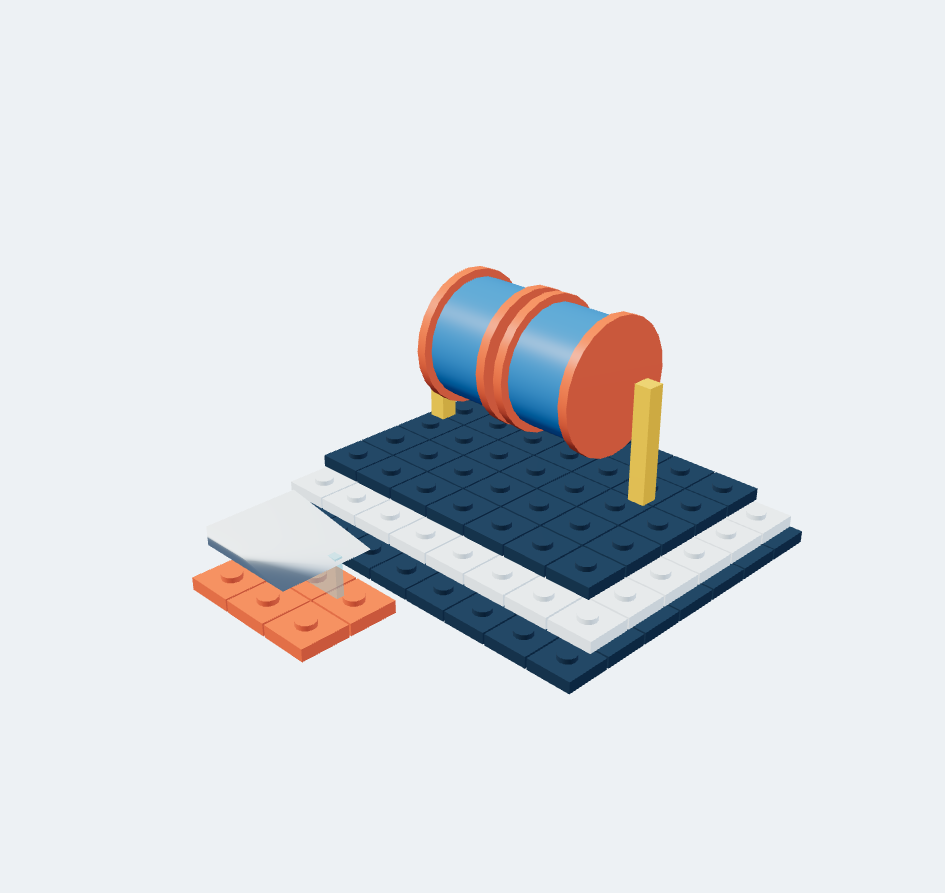
\includegraphics[width=.24\textwidth]{figures/hierarchy-expanded/exp-d2-drum-2-iso.png}
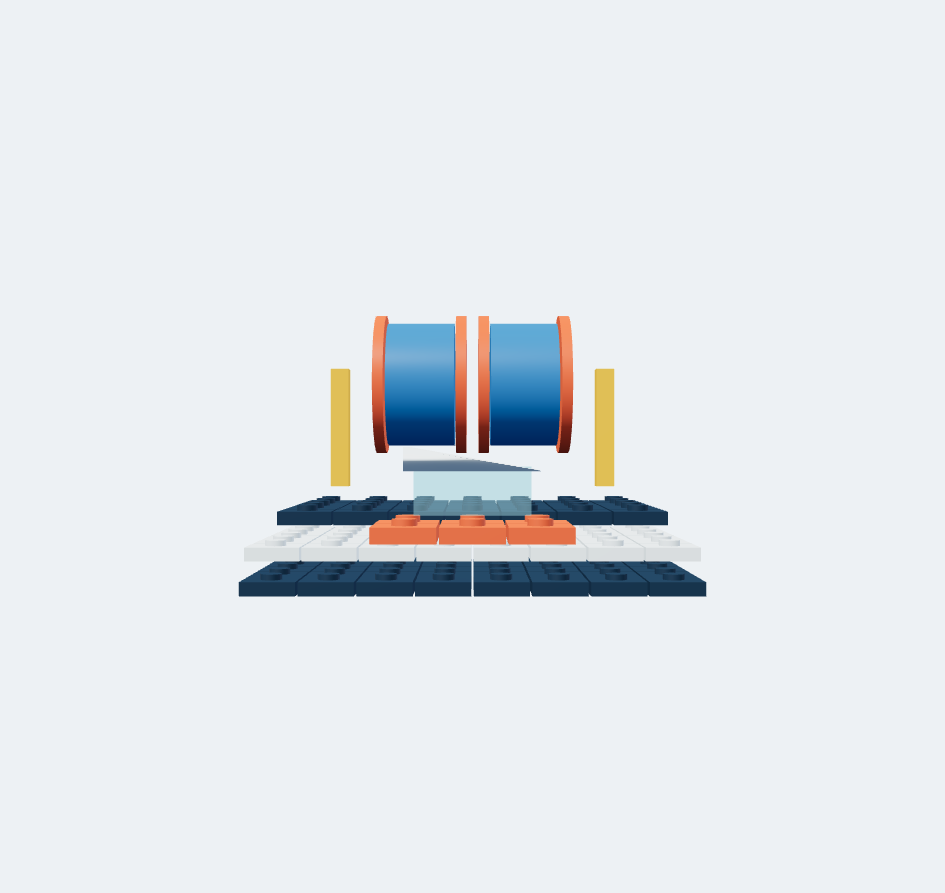
\includegraphics[width=.24\textwidth]{figures/hierarchy-expanded/exp-d2-drum-2-front.png}

\includegraphics[width=.24\textwidth]{figures/hierarchy-expanded/exp-d2-drum-2-side.png}
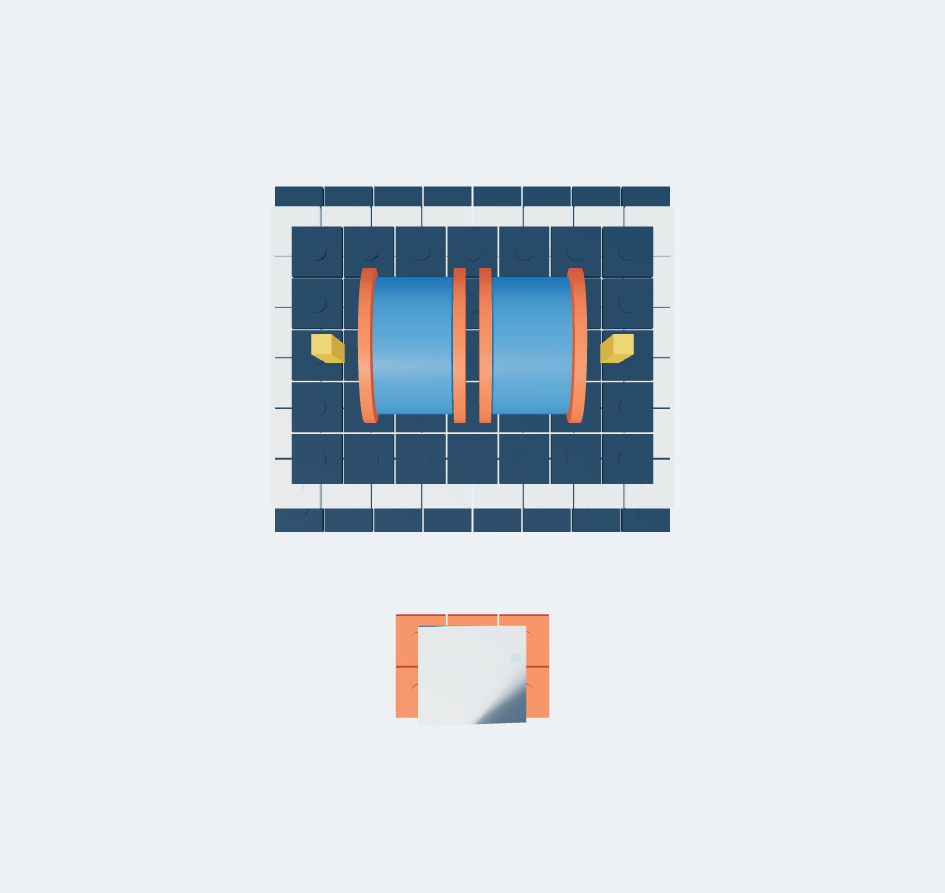
\includegraphics[width=.24\textwidth]{figures/hierarchy-expanded/exp-d2-drum-2-top.png}
\end{center}
\noindent All 48 families share this source. Full inputs and answers appear in the companion question bank.
\begin{center}\tiny\begin{tabular}{rllll}\toprule No. & Family & Layer & Output & Evidence\\\midrule
1 & identify & atomic & single-choice & model-state \\
2 & count & atomic & single-choice & model-state \\
3 & color & atomic & single-choice & model-state \\
4 & position & atomic & single-choice & model-state \\
5 & joint-type & atomic & single-choice & model-state \\
6 & parent & atomic & single-choice & model-state \\
7 & anchor & atomic & single-choice & model-state \\
8 & degree & atomic & single-choice & model-state \\
9 & recolor & atomic & single-choice & model-state \\
10 & add & atomic & single-choice & model-state \\
11 & remove & atomic & single-choice & model-state \\
12 & replace & atomic & single-choice & model-state \\
13 & translate & atomic & single-choice & model-state \\
14 & rotate & atomic & single-choice & model-state \\
15 & next-module & atomic & single-choice & model-state \\
16 & inventory & atomic & single-choice & model-state \\
17 & boundary & atomic & single-choice & model-state \\
18 & no-op & atomic & single-choice & model-state \\
19 & prefix & metacognitive & single-choice & support-graph \\
20 & access & metacognitive & multiple-choice & Rapier \\
21 & counterfactual & metacognitive & single-choice & support-graph \\
22 & dynamic & metacognitive & single-choice & Rapier \\
23 & kinematic & metacognitive & multiple-choice & model-state \\
24 & diagnosis & metacognitive & multiple-choice & model-state \\
25 & information-gain & metacognitive & multiple-choice & finite-world \\
26 & abstention & metacognitive & single-choice & finite-world \\
27 & posterior & metacognitive & single-choice & finite-world \\
28 & pareto & metacognitive & multiple-choice & model-state \\
29 & assembly & procedural & actions & state-machine \\
30 & disassembly & procedural & actions & state-machine \\
31 & service-repair & procedural & actions & state-machine \\
32 & compound-edit & procedural & actions & state-machine \\
33 & multi-fault & integrative & actions & state-machine \\
34 & scheduling & integrative & schedule & resource-schedule \\
35 & policy & integrative & policy & finite-world \\
36 & local-frame & atomic & single-choice & model-state \\
37 & projection & atomic & single-choice & model-state \\
38 & relative-order & atomic & single-choice & model-state \\
39 & joint-axis & atomic & single-choice & model-state \\
40 & clearance-margin & metacognitive & single-choice & model-state \\
41 & load-moment & metacognitive & single-choice & model-state \\
42 & weighted-posterior & metacognitive & single-choice & finite-world \\
43 & expected-loss & metacognitive & single-choice & finite-world \\
44 & trace-threshold & metacognitive & single-choice & Rapier \\
45 & guarded-repair & procedural & actions & state-machine \\
46 & rollback & procedural & actions & state-machine \\
47 & resource-repair & integrative & actions & state-machine \\
48 & budget-policy & integrative & policy & finite-world \\
\bottomrule\end{tabular}\end{center}
\clearpage
\subsection{48. Gantry Inspection Stage Assembly (D2)}
166 visible parts; 7 modules; 6 joints. Representative-point motion 0.0000; rotation 0.0000 rad.
\begin{center}
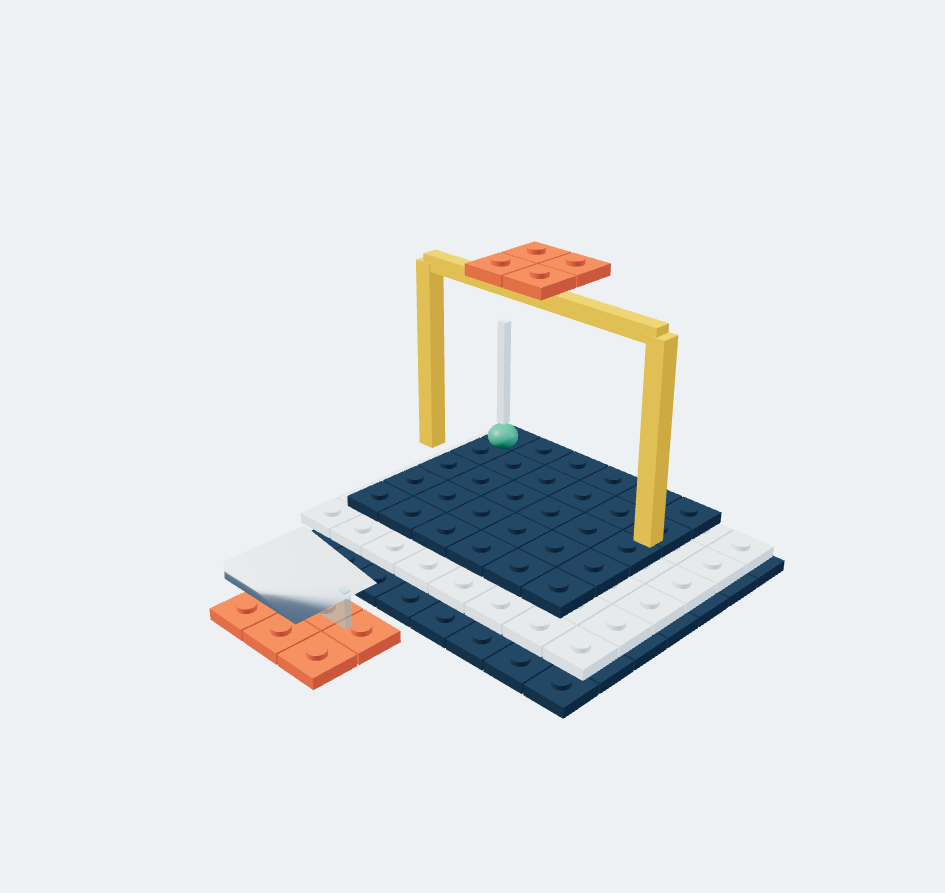
\includegraphics[width=.24\textwidth]{figures/hierarchy-expanded/exp-d2-gantry-1-iso.png}
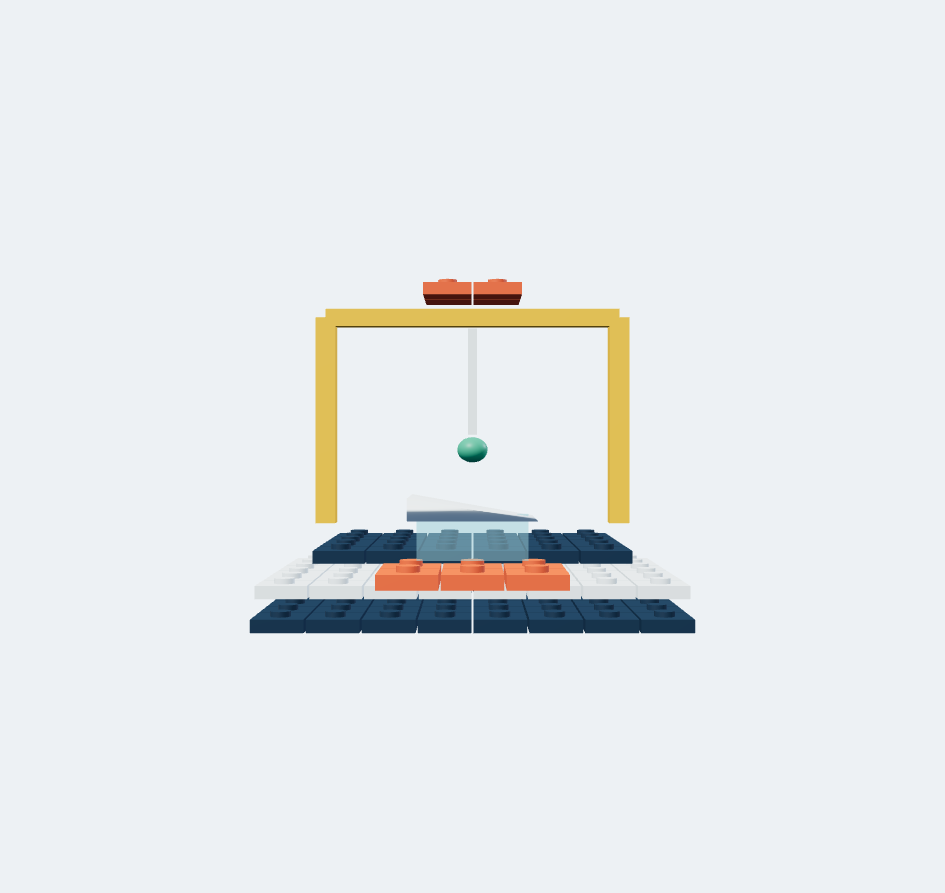
\includegraphics[width=.24\textwidth]{figures/hierarchy-expanded/exp-d2-gantry-1-front.png}
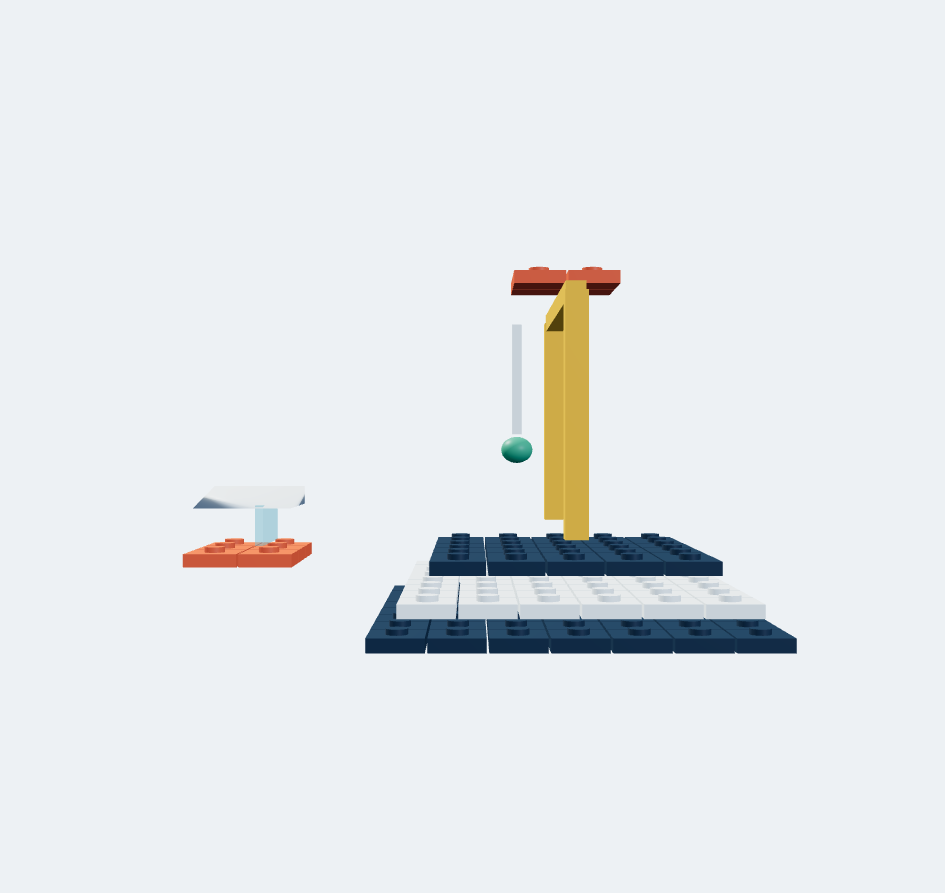
\includegraphics[width=.24\textwidth]{figures/hierarchy-expanded/exp-d2-gantry-1-side.png}
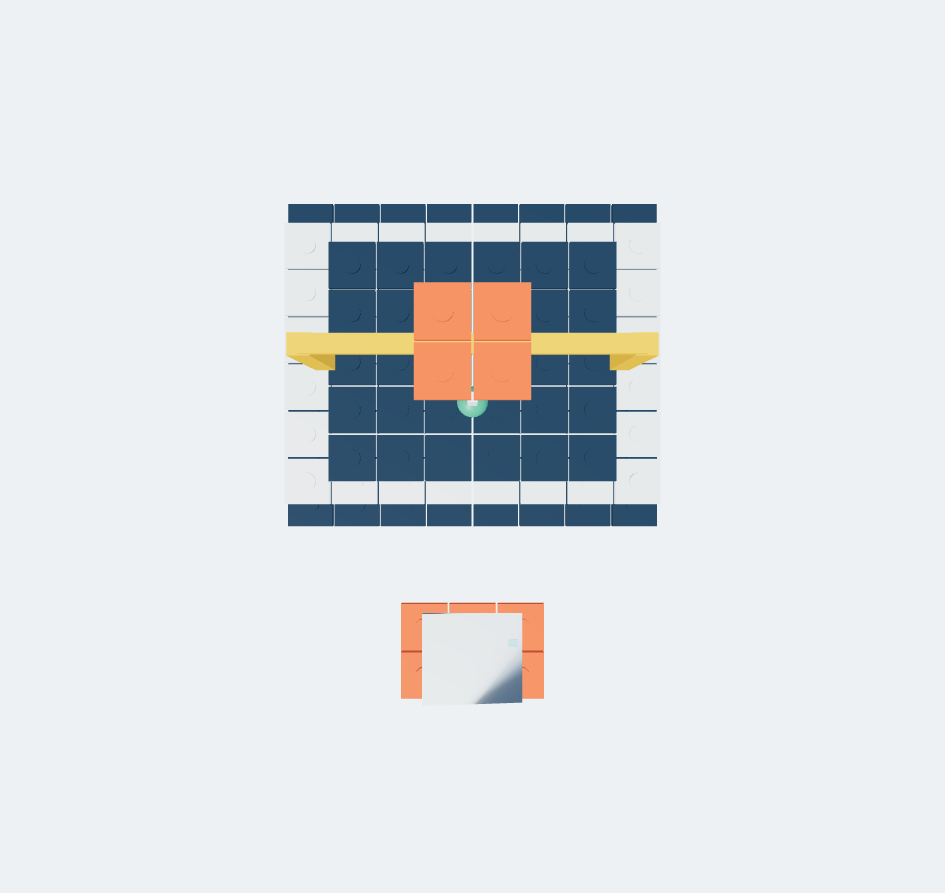
\includegraphics[width=.24\textwidth]{figures/hierarchy-expanded/exp-d2-gantry-1-top.png}
\end{center}
\noindent All 48 families share this source. Full inputs and answers appear in the companion question bank.
\begin{center}\tiny\begin{tabular}{rllll}\toprule No. & Family & Layer & Output & Evidence\\\midrule
1 & identify & atomic & single-choice & model-state \\
2 & count & atomic & single-choice & model-state \\
3 & color & atomic & single-choice & model-state \\
4 & position & atomic & single-choice & model-state \\
5 & joint-type & atomic & single-choice & model-state \\
6 & parent & atomic & single-choice & model-state \\
7 & anchor & atomic & single-choice & model-state \\
8 & degree & atomic & single-choice & model-state \\
9 & recolor & atomic & single-choice & model-state \\
10 & add & atomic & single-choice & model-state \\
11 & remove & atomic & single-choice & model-state \\
12 & replace & atomic & single-choice & model-state \\
13 & translate & atomic & single-choice & model-state \\
14 & rotate & atomic & single-choice & model-state \\
15 & next-module & atomic & single-choice & model-state \\
16 & inventory & atomic & single-choice & model-state \\
17 & boundary & atomic & single-choice & model-state \\
18 & no-op & atomic & single-choice & model-state \\
19 & prefix & metacognitive & single-choice & support-graph \\
20 & access & metacognitive & multiple-choice & Rapier \\
21 & counterfactual & metacognitive & single-choice & support-graph \\
22 & dynamic & metacognitive & single-choice & Rapier \\
23 & kinematic & metacognitive & multiple-choice & model-state \\
24 & diagnosis & metacognitive & multiple-choice & model-state \\
25 & information-gain & metacognitive & multiple-choice & finite-world \\
26 & abstention & metacognitive & single-choice & finite-world \\
27 & posterior & metacognitive & single-choice & finite-world \\
28 & pareto & metacognitive & multiple-choice & model-state \\
29 & assembly & procedural & actions & state-machine \\
30 & disassembly & procedural & actions & state-machine \\
31 & service-repair & procedural & actions & state-machine \\
32 & compound-edit & procedural & actions & state-machine \\
33 & multi-fault & integrative & actions & state-machine \\
34 & scheduling & integrative & schedule & resource-schedule \\
35 & policy & integrative & policy & finite-world \\
36 & local-frame & atomic & single-choice & model-state \\
37 & projection & atomic & single-choice & model-state \\
38 & relative-order & atomic & single-choice & model-state \\
39 & joint-axis & atomic & single-choice & model-state \\
40 & clearance-margin & metacognitive & single-choice & model-state \\
41 & load-moment & metacognitive & single-choice & model-state \\
42 & weighted-posterior & metacognitive & single-choice & finite-world \\
43 & expected-loss & metacognitive & single-choice & finite-world \\
44 & trace-threshold & metacognitive & single-choice & Rapier \\
45 & guarded-repair & procedural & actions & state-machine \\
46 & rollback & procedural & actions & state-machine \\
47 & resource-repair & integrative & actions & state-machine \\
48 & budget-policy & integrative & policy & finite-world \\
\bottomrule\end{tabular}\end{center}
\clearpage
\subsection{49. Twin-trolley Service Frame Assembly (D2)}
179 visible parts; 9 modules; 8 joints. Representative-point motion 0.0000; rotation 0.0000 rad.
\begin{center}
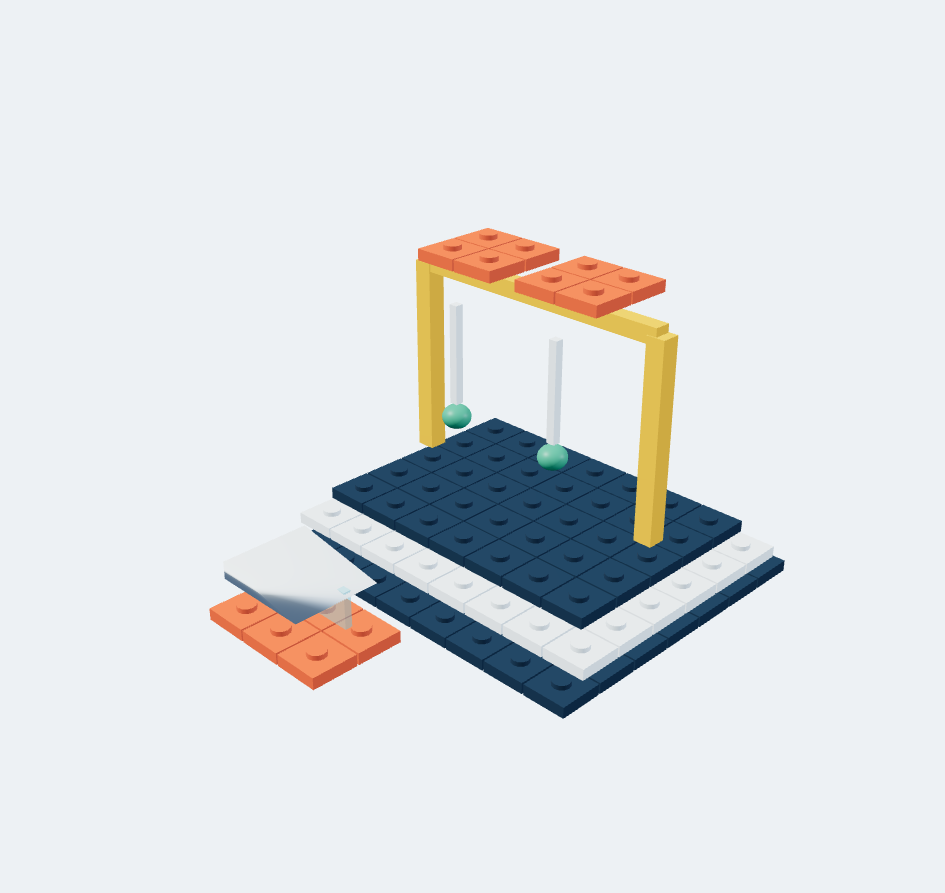
\includegraphics[width=.24\textwidth]{figures/hierarchy-expanded/exp-d2-gantry-2-iso.png}
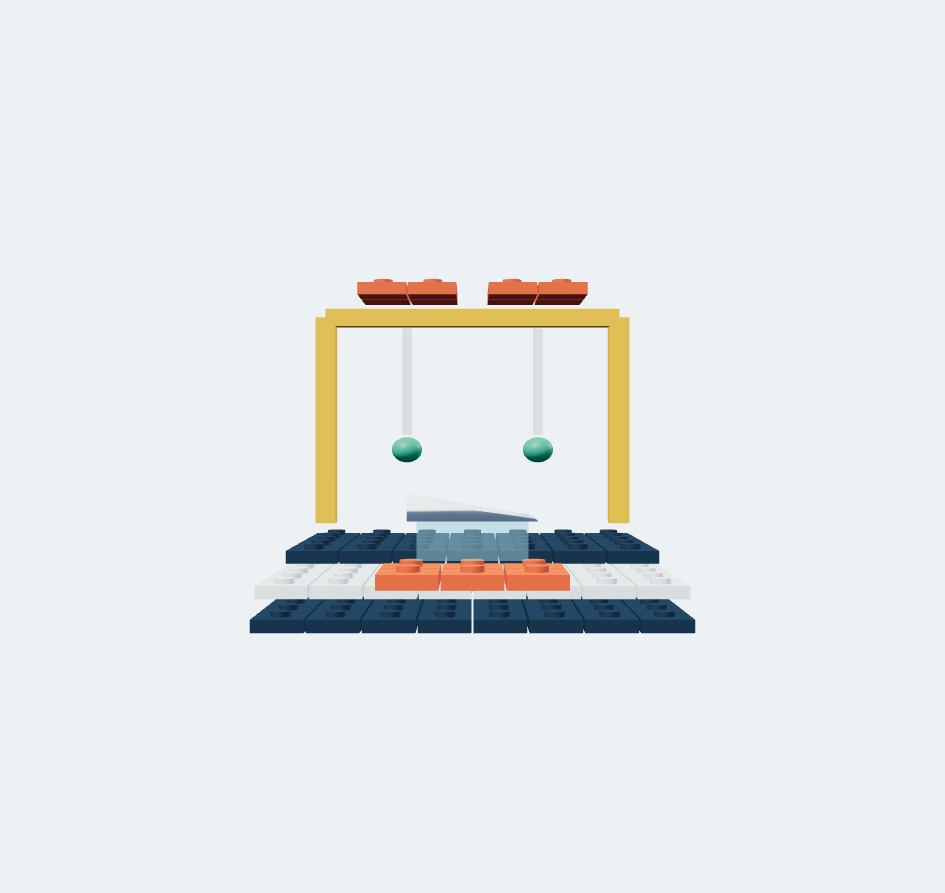
\includegraphics[width=.24\textwidth]{figures/hierarchy-expanded/exp-d2-gantry-2-front.png}
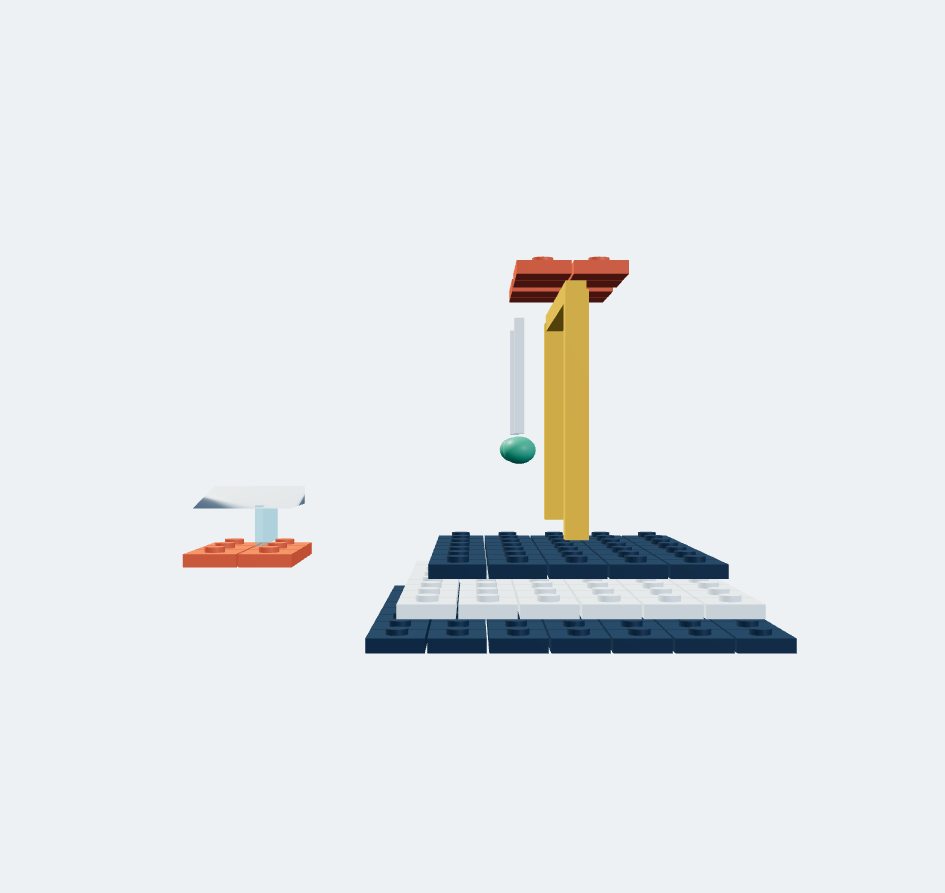
\includegraphics[width=.24\textwidth]{figures/hierarchy-expanded/exp-d2-gantry-2-side.png}
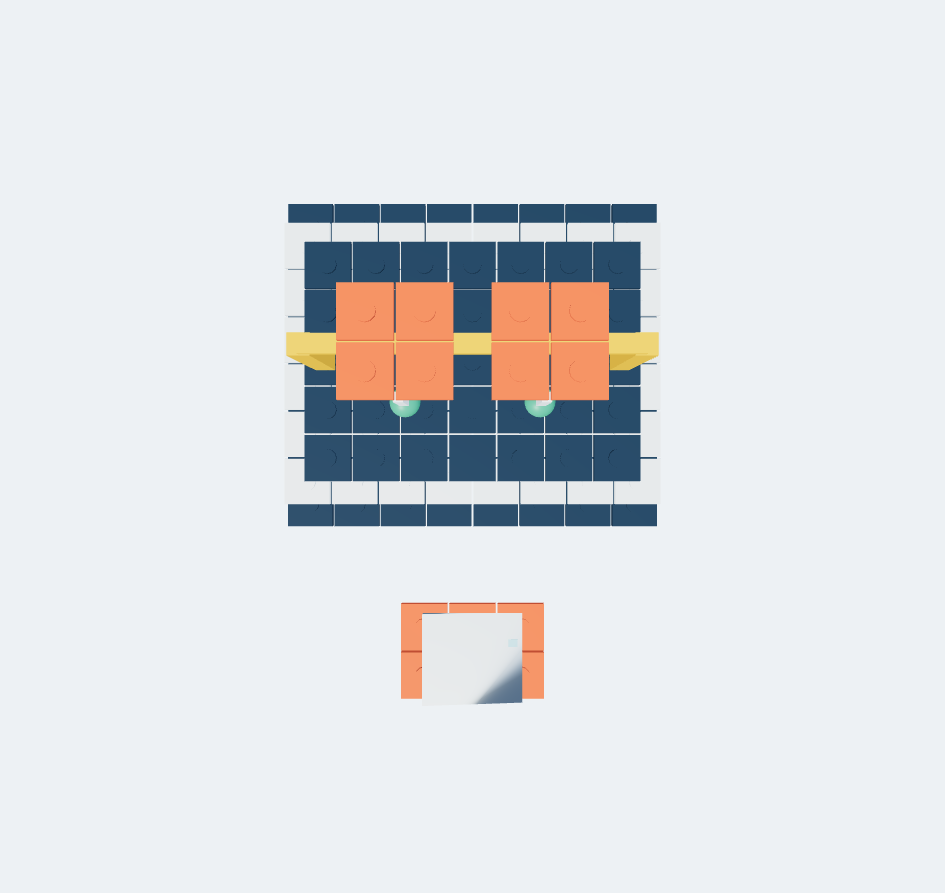
\includegraphics[width=.24\textwidth]{figures/hierarchy-expanded/exp-d2-gantry-2-top.png}
\end{center}
\noindent All 48 families share this source. Full inputs and answers appear in the companion question bank.
\begin{center}\tiny\begin{tabular}{rllll}\toprule No. & Family & Layer & Output & Evidence\\\midrule
1 & identify & atomic & single-choice & model-state \\
2 & count & atomic & single-choice & model-state \\
3 & color & atomic & single-choice & model-state \\
4 & position & atomic & single-choice & model-state \\
5 & joint-type & atomic & single-choice & model-state \\
6 & parent & atomic & single-choice & model-state \\
7 & anchor & atomic & single-choice & model-state \\
8 & degree & atomic & single-choice & model-state \\
9 & recolor & atomic & single-choice & model-state \\
10 & add & atomic & single-choice & model-state \\
11 & remove & atomic & single-choice & model-state \\
12 & replace & atomic & single-choice & model-state \\
13 & translate & atomic & single-choice & model-state \\
14 & rotate & atomic & single-choice & model-state \\
15 & next-module & atomic & single-choice & model-state \\
16 & inventory & atomic & single-choice & model-state \\
17 & boundary & atomic & single-choice & model-state \\
18 & no-op & atomic & single-choice & model-state \\
19 & prefix & metacognitive & single-choice & support-graph \\
20 & access & metacognitive & multiple-choice & Rapier \\
21 & counterfactual & metacognitive & single-choice & support-graph \\
22 & dynamic & metacognitive & single-choice & Rapier \\
23 & kinematic & metacognitive & multiple-choice & model-state \\
24 & diagnosis & metacognitive & multiple-choice & model-state \\
25 & information-gain & metacognitive & multiple-choice & finite-world \\
26 & abstention & metacognitive & single-choice & finite-world \\
27 & posterior & metacognitive & single-choice & finite-world \\
28 & pareto & metacognitive & multiple-choice & model-state \\
29 & assembly & procedural & actions & state-machine \\
30 & disassembly & procedural & actions & state-machine \\
31 & service-repair & procedural & actions & state-machine \\
32 & compound-edit & procedural & actions & state-machine \\
33 & multi-fault & integrative & actions & state-machine \\
34 & scheduling & integrative & schedule & resource-schedule \\
35 & policy & integrative & policy & finite-world \\
36 & local-frame & atomic & single-choice & model-state \\
37 & projection & atomic & single-choice & model-state \\
38 & relative-order & atomic & single-choice & model-state \\
39 & joint-axis & atomic & single-choice & model-state \\
40 & clearance-margin & metacognitive & single-choice & model-state \\
41 & load-moment & metacognitive & single-choice & model-state \\
42 & weighted-posterior & metacognitive & single-choice & finite-world \\
43 & expected-loss & metacognitive & single-choice & finite-world \\
44 & trace-threshold & metacognitive & single-choice & Rapier \\
45 & guarded-repair & procedural & actions & state-machine \\
46 & rollback & procedural & actions & state-machine \\
47 & resource-repair & integrative & actions & state-machine \\
48 & budget-policy & integrative & policy & finite-world \\
\bottomrule\end{tabular}\end{center}
\clearpage
\subsection{50. Rotary Sector Gate Assembly (D2)}
159 visible parts; 5 modules; 4 joints. Representative-point motion 0.0000; rotation 0.0000 rad.
\begin{center}
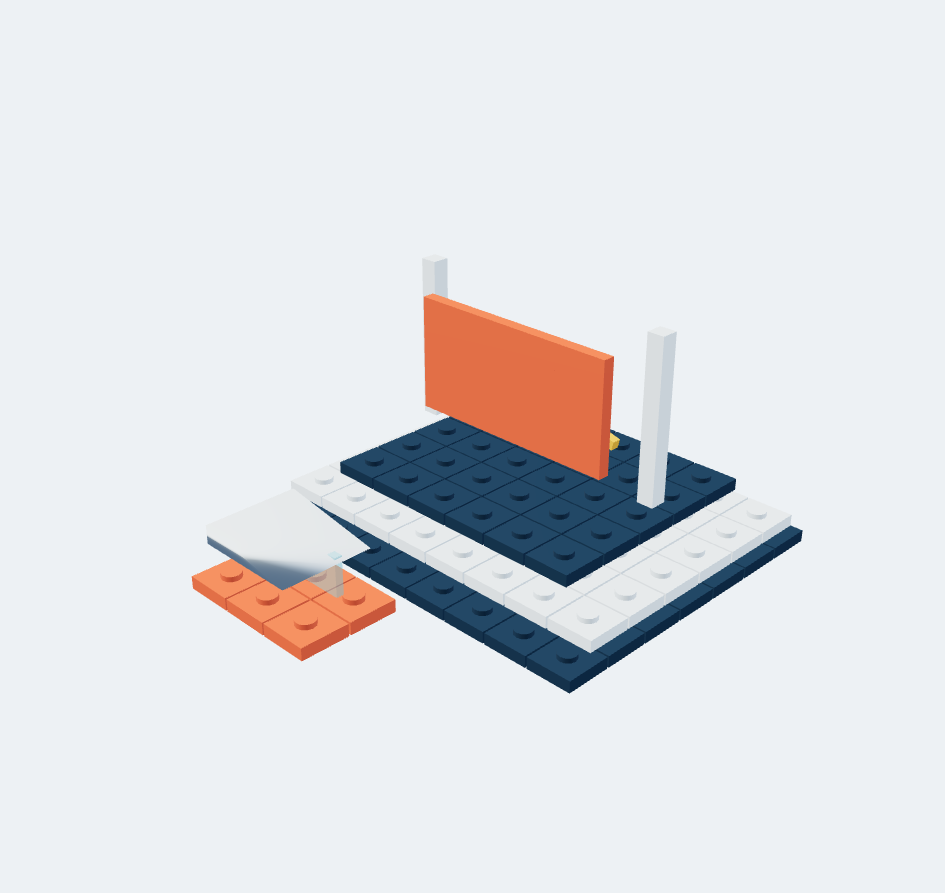
\includegraphics[width=.24\textwidth]{figures/hierarchy-expanded/exp-d2-gate-1-iso.png}

\includegraphics[width=.24\textwidth]{figures/hierarchy-expanded/exp-d2-gate-1-front.png}
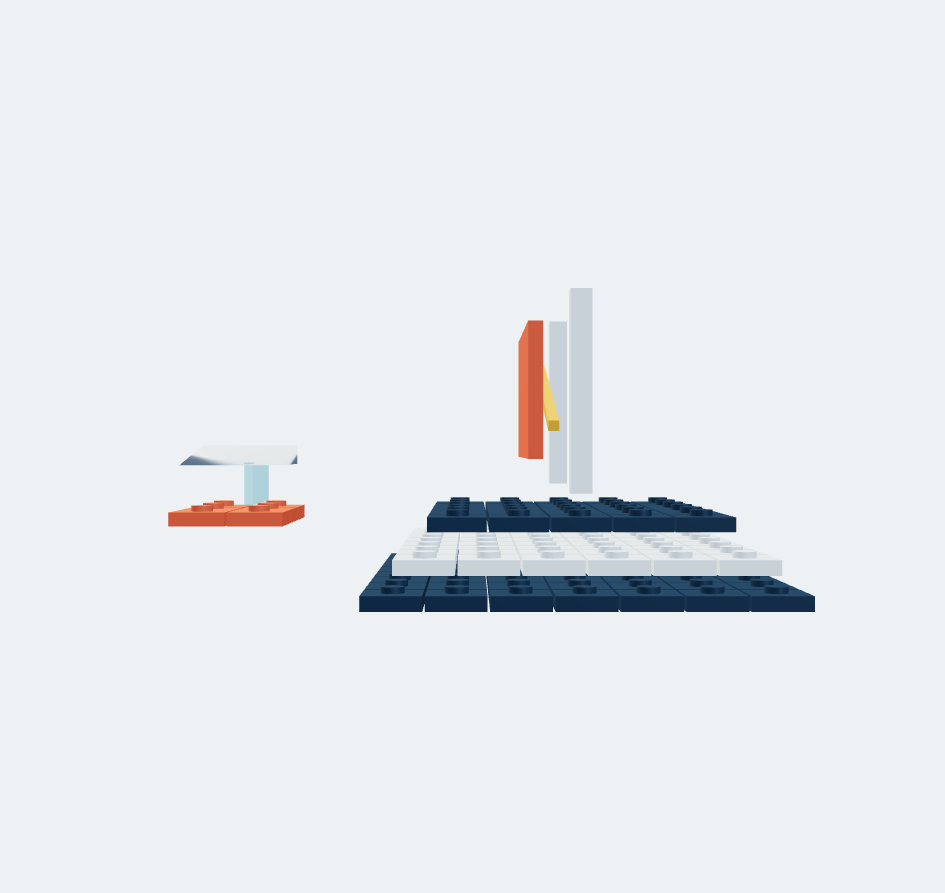
\includegraphics[width=.24\textwidth]{figures/hierarchy-expanded/exp-d2-gate-1-side.png}
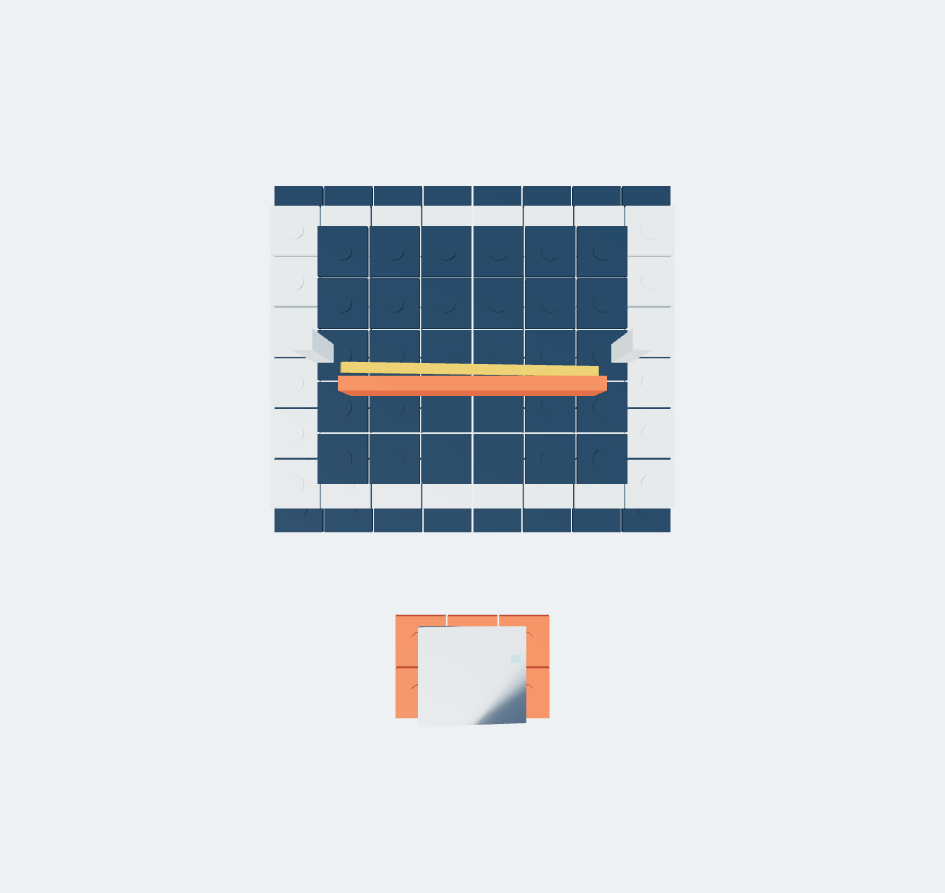
\includegraphics[width=.24\textwidth]{figures/hierarchy-expanded/exp-d2-gate-1-top.png}
\end{center}
\noindent All 48 families share this source. Full inputs and answers appear in the companion question bank.
\begin{center}\tiny\begin{tabular}{rllll}\toprule No. & Family & Layer & Output & Evidence\\\midrule
1 & identify & atomic & single-choice & model-state \\
2 & count & atomic & single-choice & model-state \\
3 & color & atomic & single-choice & model-state \\
4 & position & atomic & single-choice & model-state \\
5 & joint-type & atomic & single-choice & model-state \\
6 & parent & atomic & single-choice & model-state \\
7 & anchor & atomic & single-choice & model-state \\
8 & degree & atomic & single-choice & model-state \\
9 & recolor & atomic & single-choice & model-state \\
10 & add & atomic & single-choice & model-state \\
11 & remove & atomic & single-choice & model-state \\
12 & replace & atomic & single-choice & model-state \\
13 & translate & atomic & single-choice & model-state \\
14 & rotate & atomic & single-choice & model-state \\
15 & next-module & atomic & single-choice & model-state \\
16 & inventory & atomic & single-choice & model-state \\
17 & boundary & atomic & single-choice & model-state \\
18 & no-op & atomic & single-choice & model-state \\
19 & prefix & metacognitive & single-choice & support-graph \\
20 & access & metacognitive & multiple-choice & Rapier \\
21 & counterfactual & metacognitive & single-choice & support-graph \\
22 & dynamic & metacognitive & single-choice & Rapier \\
23 & kinematic & metacognitive & multiple-choice & model-state \\
24 & diagnosis & metacognitive & multiple-choice & model-state \\
25 & information-gain & metacognitive & multiple-choice & finite-world \\
26 & abstention & metacognitive & single-choice & finite-world \\
27 & posterior & metacognitive & single-choice & finite-world \\
28 & pareto & metacognitive & multiple-choice & model-state \\
29 & assembly & procedural & actions & state-machine \\
30 & disassembly & procedural & actions & state-machine \\
31 & service-repair & procedural & actions & state-machine \\
32 & compound-edit & procedural & actions & state-machine \\
33 & multi-fault & integrative & actions & state-machine \\
34 & scheduling & integrative & schedule & resource-schedule \\
35 & policy & integrative & policy & finite-world \\
36 & local-frame & atomic & single-choice & model-state \\
37 & projection & atomic & single-choice & model-state \\
38 & relative-order & atomic & single-choice & model-state \\
39 & joint-axis & atomic & single-choice & model-state \\
40 & clearance-margin & metacognitive & single-choice & model-state \\
41 & load-moment & metacognitive & single-choice & model-state \\
42 & weighted-posterior & metacognitive & single-choice & finite-world \\
43 & expected-loss & metacognitive & single-choice & finite-world \\
44 & trace-threshold & metacognitive & single-choice & Rapier \\
45 & guarded-repair & procedural & actions & state-machine \\
46 & rollback & procedural & actions & state-machine \\
47 & resource-repair & integrative & actions & state-machine \\
48 & budget-policy & integrative & policy & finite-world \\
\bottomrule\end{tabular}\end{center}
\clearpage
\subsection{51. Twin-leaf Interlock Frame Assembly (D2)}
169 visible parts; 6 modules; 5 joints. Representative-point motion 0.0000; rotation 0.0000 rad.
\begin{center}
\includegraphics[width=.24\textwidth]{figures/hierarchy-expanded/exp-d2-gate-2-iso.png}
\includegraphics[width=.24\textwidth]{figures/hierarchy-expanded/exp-d2-gate-2-front.png}
\includegraphics[width=.24\textwidth]{figures/hierarchy-expanded/exp-d2-gate-2-side.png}
\includegraphics[width=.24\textwidth]{figures/hierarchy-expanded/exp-d2-gate-2-top.png}
\end{center}
\noindent All 48 families share this source. Full inputs and answers appear in the companion question bank.
\begin{center}\tiny\begin{tabular}{rllll}\toprule No. & Family & Layer & Output & Evidence\\\midrule
1 & identify & atomic & single-choice & model-state \\
2 & count & atomic & single-choice & model-state \\
3 & color & atomic & single-choice & model-state \\
4 & position & atomic & single-choice & model-state \\
5 & joint-type & atomic & single-choice & model-state \\
6 & parent & atomic & single-choice & model-state \\
7 & anchor & atomic & single-choice & model-state \\
8 & degree & atomic & single-choice & model-state \\
9 & recolor & atomic & single-choice & model-state \\
10 & add & atomic & single-choice & model-state \\
11 & remove & atomic & single-choice & model-state \\
12 & replace & atomic & single-choice & model-state \\
13 & translate & atomic & single-choice & model-state \\
14 & rotate & atomic & single-choice & model-state \\
15 & next-module & atomic & single-choice & model-state \\
16 & inventory & atomic & single-choice & model-state \\
17 & boundary & atomic & single-choice & model-state \\
18 & no-op & atomic & single-choice & model-state \\
19 & prefix & metacognitive & single-choice & support-graph \\
20 & access & metacognitive & multiple-choice & Rapier \\
21 & counterfactual & metacognitive & single-choice & support-graph \\
22 & dynamic & metacognitive & single-choice & Rapier \\
23 & kinematic & metacognitive & multiple-choice & model-state \\
24 & diagnosis & metacognitive & multiple-choice & model-state \\
25 & information-gain & metacognitive & multiple-choice & finite-world \\
26 & abstention & metacognitive & single-choice & finite-world \\
27 & posterior & metacognitive & single-choice & finite-world \\
28 & pareto & metacognitive & multiple-choice & model-state \\
29 & assembly & procedural & actions & state-machine \\
30 & disassembly & procedural & actions & state-machine \\
31 & service-repair & procedural & actions & state-machine \\
32 & compound-edit & procedural & actions & state-machine \\
33 & multi-fault & integrative & actions & state-machine \\
34 & scheduling & integrative & schedule & resource-schedule \\
35 & policy & integrative & policy & finite-world \\
36 & local-frame & atomic & single-choice & model-state \\
37 & projection & atomic & single-choice & model-state \\
38 & relative-order & atomic & single-choice & model-state \\
39 & joint-axis & atomic & single-choice & model-state \\
40 & clearance-margin & metacognitive & single-choice & model-state \\
41 & load-moment & metacognitive & single-choice & model-state \\
42 & weighted-posterior & metacognitive & single-choice & finite-world \\
43 & expected-loss & metacognitive & single-choice & finite-world \\
44 & trace-threshold & metacognitive & single-choice & Rapier \\
45 & guarded-repair & procedural & actions & state-machine \\
46 & rollback & procedural & actions & state-machine \\
47 & resource-repair & integrative & actions & state-machine \\
48 & budget-policy & integrative & policy & finite-world \\
\bottomrule\end{tabular}\end{center}
\clearpage
\subsection{52. Opposed Gripper Assembly (D2)}
149 visible parts; 7 modules; 6 joints. Representative-point motion 0.0001; rotation 0.0000 rad.
\begin{center}
\includegraphics[width=.24\textwidth]{figures/hierarchy-expanded/exp-d2-gripper-1-iso.png}
\includegraphics[width=.24\textwidth]{figures/hierarchy-expanded/exp-d2-gripper-1-front.png}
\includegraphics[width=.24\textwidth]{figures/hierarchy-expanded/exp-d2-gripper-1-side.png}
\includegraphics[width=.24\textwidth]{figures/hierarchy-expanded/exp-d2-gripper-1-top.png}
\end{center}
\noindent All 48 families share this source. Full inputs and answers appear in the companion question bank.
\begin{center}\tiny\begin{tabular}{rllll}\toprule No. & Family & Layer & Output & Evidence\\\midrule
1 & identify & atomic & single-choice & model-state \\
2 & count & atomic & single-choice & model-state \\
3 & color & atomic & single-choice & model-state \\
4 & position & atomic & single-choice & model-state \\
5 & joint-type & atomic & single-choice & model-state \\
6 & parent & atomic & single-choice & model-state \\
7 & anchor & atomic & single-choice & model-state \\
8 & degree & atomic & single-choice & model-state \\
9 & recolor & atomic & single-choice & model-state \\
10 & add & atomic & single-choice & model-state \\
11 & remove & atomic & single-choice & model-state \\
12 & replace & atomic & single-choice & model-state \\
13 & translate & atomic & single-choice & model-state \\
14 & rotate & atomic & single-choice & model-state \\
15 & next-module & atomic & single-choice & model-state \\
16 & inventory & atomic & single-choice & model-state \\
17 & boundary & atomic & single-choice & model-state \\
18 & no-op & atomic & single-choice & model-state \\
19 & prefix & metacognitive & single-choice & support-graph \\
20 & access & metacognitive & multiple-choice & Rapier \\
21 & counterfactual & metacognitive & single-choice & support-graph \\
22 & dynamic & metacognitive & single-choice & Rapier \\
23 & kinematic & metacognitive & multiple-choice & model-state \\
24 & diagnosis & metacognitive & multiple-choice & model-state \\
25 & information-gain & metacognitive & multiple-choice & finite-world \\
26 & abstention & metacognitive & single-choice & finite-world \\
27 & posterior & metacognitive & single-choice & finite-world \\
28 & pareto & metacognitive & multiple-choice & model-state \\
29 & assembly & procedural & actions & state-machine \\
30 & disassembly & procedural & actions & state-machine \\
31 & service-repair & procedural & actions & state-machine \\
32 & compound-edit & procedural & actions & state-machine \\
33 & multi-fault & integrative & actions & state-machine \\
34 & scheduling & integrative & schedule & resource-schedule \\
35 & policy & integrative & policy & finite-world \\
36 & local-frame & atomic & single-choice & model-state \\
37 & projection & atomic & single-choice & model-state \\
38 & relative-order & atomic & single-choice & model-state \\
39 & joint-axis & atomic & single-choice & model-state \\
40 & clearance-margin & metacognitive & single-choice & model-state \\
41 & load-moment & metacognitive & single-choice & model-state \\
42 & weighted-posterior & metacognitive & single-choice & finite-world \\
43 & expected-loss & metacognitive & single-choice & finite-world \\
44 & trace-threshold & metacognitive & single-choice & Rapier \\
45 & guarded-repair & procedural & actions & state-machine \\
46 & rollback & procedural & actions & state-machine \\
47 & resource-repair & integrative & actions & state-machine \\
48 & budget-policy & integrative & policy & finite-world \\
\bottomrule\end{tabular}\end{center}
\clearpage
\subsection{53. Three-finger Gripper Assembly (D2)}
157 visible parts; 8 modules; 7 joints. Representative-point motion 0.0001; rotation 0.0000 rad.
\begin{center}
\includegraphics[width=.24\textwidth]{figures/hierarchy-expanded/exp-d2-gripper-2-iso.png}
\includegraphics[width=.24\textwidth]{figures/hierarchy-expanded/exp-d2-gripper-2-front.png}
\includegraphics[width=.24\textwidth]{figures/hierarchy-expanded/exp-d2-gripper-2-side.png}
\includegraphics[width=.24\textwidth]{figures/hierarchy-expanded/exp-d2-gripper-2-top.png}
\end{center}
\noindent All 48 families share this source. Full inputs and answers appear in the companion question bank.
\begin{center}\tiny\begin{tabular}{rllll}\toprule No. & Family & Layer & Output & Evidence\\\midrule
1 & identify & atomic & single-choice & model-state \\
2 & count & atomic & single-choice & model-state \\
3 & color & atomic & single-choice & model-state \\
4 & position & atomic & single-choice & model-state \\
5 & joint-type & atomic & single-choice & model-state \\
6 & parent & atomic & single-choice & model-state \\
7 & anchor & atomic & single-choice & model-state \\
8 & degree & atomic & single-choice & model-state \\
9 & recolor & atomic & single-choice & model-state \\
10 & add & atomic & single-choice & model-state \\
11 & remove & atomic & single-choice & model-state \\
12 & replace & atomic & single-choice & model-state \\
13 & translate & atomic & single-choice & model-state \\
14 & rotate & atomic & single-choice & model-state \\
15 & next-module & atomic & single-choice & model-state \\
16 & inventory & atomic & single-choice & model-state \\
17 & boundary & atomic & single-choice & model-state \\
18 & no-op & atomic & single-choice & model-state \\
19 & prefix & metacognitive & single-choice & support-graph \\
20 & access & metacognitive & multiple-choice & Rapier \\
21 & counterfactual & metacognitive & single-choice & support-graph \\
22 & dynamic & metacognitive & single-choice & Rapier \\
23 & kinematic & metacognitive & multiple-choice & model-state \\
24 & diagnosis & metacognitive & multiple-choice & model-state \\
25 & information-gain & metacognitive & multiple-choice & finite-world \\
26 & abstention & metacognitive & single-choice & finite-world \\
27 & posterior & metacognitive & single-choice & finite-world \\
28 & pareto & metacognitive & multiple-choice & model-state \\
29 & assembly & procedural & actions & state-machine \\
30 & disassembly & procedural & actions & state-machine \\
31 & service-repair & procedural & actions & state-machine \\
32 & compound-edit & procedural & actions & state-machine \\
33 & multi-fault & integrative & actions & state-machine \\
34 & scheduling & integrative & schedule & resource-schedule \\
35 & policy & integrative & policy & finite-world \\
36 & local-frame & atomic & single-choice & model-state \\
37 & projection & atomic & single-choice & model-state \\
38 & relative-order & atomic & single-choice & model-state \\
39 & joint-axis & atomic & single-choice & model-state \\
40 & clearance-margin & metacognitive & single-choice & model-state \\
41 & load-moment & metacognitive & single-choice & model-state \\
42 & weighted-posterior & metacognitive & single-choice & finite-world \\
43 & expected-loss & metacognitive & single-choice & finite-world \\
44 & trace-threshold & metacognitive & single-choice & Rapier \\
45 & guarded-repair & procedural & actions & state-machine \\
46 & rollback & procedural & actions & state-machine \\
47 & resource-repair & integrative & actions & state-machine \\
48 & budget-policy & integrative & policy & finite-world \\
\bottomrule\end{tabular}\end{center}
\clearpage
\subsection{54. Inclined Probe Stand Assembly (D2)}
147 visible parts; 6 modules; 5 joints. Representative-point motion 0.0000; rotation 0.0000 rad.
\begin{center}
\includegraphics[width=.24\textwidth]{figures/hierarchy-expanded/exp-d2-probe-1-iso.png}
\includegraphics[width=.24\textwidth]{figures/hierarchy-expanded/exp-d2-probe-1-front.png}
\includegraphics[width=.24\textwidth]{figures/hierarchy-expanded/exp-d2-probe-1-side.png}
\includegraphics[width=.24\textwidth]{figures/hierarchy-expanded/exp-d2-probe-1-top.png}
\end{center}
\noindent All 48 families share this source. Full inputs and answers appear in the companion question bank.
\begin{center}\tiny\begin{tabular}{rllll}\toprule No. & Family & Layer & Output & Evidence\\\midrule
1 & identify & atomic & single-choice & model-state \\
2 & count & atomic & single-choice & model-state \\
3 & color & atomic & single-choice & model-state \\
4 & position & atomic & single-choice & model-state \\
5 & joint-type & atomic & single-choice & model-state \\
6 & parent & atomic & single-choice & model-state \\
7 & anchor & atomic & single-choice & model-state \\
8 & degree & atomic & single-choice & model-state \\
9 & recolor & atomic & single-choice & model-state \\
10 & add & atomic & single-choice & model-state \\
11 & remove & atomic & single-choice & model-state \\
12 & replace & atomic & single-choice & model-state \\
13 & translate & atomic & single-choice & model-state \\
14 & rotate & atomic & single-choice & model-state \\
15 & next-module & atomic & single-choice & model-state \\
16 & inventory & atomic & single-choice & model-state \\
17 & boundary & atomic & single-choice & model-state \\
18 & no-op & atomic & single-choice & model-state \\
19 & prefix & metacognitive & single-choice & support-graph \\
20 & access & metacognitive & multiple-choice & Rapier \\
21 & counterfactual & metacognitive & single-choice & support-graph \\
22 & dynamic & metacognitive & single-choice & Rapier \\
23 & kinematic & metacognitive & multiple-choice & model-state \\
24 & diagnosis & metacognitive & multiple-choice & model-state \\
25 & information-gain & metacognitive & multiple-choice & finite-world \\
26 & abstention & metacognitive & single-choice & finite-world \\
27 & posterior & metacognitive & single-choice & finite-world \\
28 & pareto & metacognitive & multiple-choice & model-state \\
29 & assembly & procedural & actions & state-machine \\
30 & disassembly & procedural & actions & state-machine \\
31 & service-repair & procedural & actions & state-machine \\
32 & compound-edit & procedural & actions & state-machine \\
33 & multi-fault & integrative & actions & state-machine \\
34 & scheduling & integrative & schedule & resource-schedule \\
35 & policy & integrative & policy & finite-world \\
36 & local-frame & atomic & single-choice & model-state \\
37 & projection & atomic & single-choice & model-state \\
38 & relative-order & atomic & single-choice & model-state \\
39 & joint-axis & atomic & single-choice & model-state \\
40 & clearance-margin & metacognitive & single-choice & model-state \\
41 & load-moment & metacognitive & single-choice & model-state \\
42 & weighted-posterior & metacognitive & single-choice & finite-world \\
43 & expected-loss & metacognitive & single-choice & finite-world \\
44 & trace-threshold & metacognitive & single-choice & Rapier \\
45 & guarded-repair & procedural & actions & state-machine \\
46 & rollback & procedural & actions & state-machine \\
47 & resource-repair & integrative & actions & state-machine \\
48 & budget-policy & integrative & policy & finite-world \\
\bottomrule\end{tabular}\end{center}
\clearpage
\subsection{55. Three-direction Probe Stand Assembly (D2)}
160 visible parts; 8 modules; 7 joints. Representative-point motion 0.0000; rotation 0.0000 rad.
\begin{center}
\includegraphics[width=.24\textwidth]{figures/hierarchy-expanded/exp-d2-probe-2-iso.png}
\includegraphics[width=.24\textwidth]{figures/hierarchy-expanded/exp-d2-probe-2-front.png}
\includegraphics[width=.24\textwidth]{figures/hierarchy-expanded/exp-d2-probe-2-side.png}
\includegraphics[width=.24\textwidth]{figures/hierarchy-expanded/exp-d2-probe-2-top.png}
\end{center}
\noindent All 48 families share this source. Full inputs and answers appear in the companion question bank.
\begin{center}\tiny\begin{tabular}{rllll}\toprule No. & Family & Layer & Output & Evidence\\\midrule
1 & identify & atomic & single-choice & model-state \\
2 & count & atomic & single-choice & model-state \\
3 & color & atomic & single-choice & model-state \\
4 & position & atomic & single-choice & model-state \\
5 & joint-type & atomic & single-choice & model-state \\
6 & parent & atomic & single-choice & model-state \\
7 & anchor & atomic & single-choice & model-state \\
8 & degree & atomic & single-choice & model-state \\
9 & recolor & atomic & single-choice & model-state \\
10 & add & atomic & single-choice & model-state \\
11 & remove & atomic & single-choice & model-state \\
12 & replace & atomic & single-choice & model-state \\
13 & translate & atomic & single-choice & model-state \\
14 & rotate & atomic & single-choice & model-state \\
15 & next-module & atomic & single-choice & model-state \\
16 & inventory & atomic & single-choice & model-state \\
17 & boundary & atomic & single-choice & model-state \\
18 & no-op & atomic & single-choice & model-state \\
19 & prefix & metacognitive & single-choice & support-graph \\
20 & access & metacognitive & multiple-choice & Rapier \\
21 & counterfactual & metacognitive & single-choice & support-graph \\
22 & dynamic & metacognitive & single-choice & Rapier \\
23 & kinematic & metacognitive & multiple-choice & model-state \\
24 & diagnosis & metacognitive & multiple-choice & model-state \\
25 & information-gain & metacognitive & multiple-choice & finite-world \\
26 & abstention & metacognitive & single-choice & finite-world \\
27 & posterior & metacognitive & single-choice & finite-world \\
28 & pareto & metacognitive & multiple-choice & model-state \\
29 & assembly & procedural & actions & state-machine \\
30 & disassembly & procedural & actions & state-machine \\
31 & service-repair & procedural & actions & state-machine \\
32 & compound-edit & procedural & actions & state-machine \\
33 & multi-fault & integrative & actions & state-machine \\
34 & scheduling & integrative & schedule & resource-schedule \\
35 & policy & integrative & policy & finite-world \\
36 & local-frame & atomic & single-choice & model-state \\
37 & projection & atomic & single-choice & model-state \\
38 & relative-order & atomic & single-choice & model-state \\
39 & joint-axis & atomic & single-choice & model-state \\
40 & clearance-margin & metacognitive & single-choice & model-state \\
41 & load-moment & metacognitive & single-choice & model-state \\
42 & weighted-posterior & metacognitive & single-choice & finite-world \\
43 & expected-loss & metacognitive & single-choice & finite-world \\
44 & trace-threshold & metacognitive & single-choice & Rapier \\
45 & guarded-repair & procedural & actions & state-machine \\
46 & rollback & procedural & actions & state-machine \\
47 & resource-repair & integrative & actions & state-machine \\
48 & budget-policy & integrative & policy & finite-world \\
\bottomrule\end{tabular}\end{center}
\clearpage
\subsection{56. Cross-feed Stage Assembly (D2)}
164 visible parts; 6 modules; 5 joints. Representative-point motion 0.0000; rotation 0.0000 rad.
\begin{center}
\includegraphics[width=.24\textwidth]{figures/hierarchy-expanded/exp-d2-slide-1-iso.png}
\includegraphics[width=.24\textwidth]{figures/hierarchy-expanded/exp-d2-slide-1-front.png}
\includegraphics[width=.24\textwidth]{figures/hierarchy-expanded/exp-d2-slide-1-side.png}
\includegraphics[width=.24\textwidth]{figures/hierarchy-expanded/exp-d2-slide-1-top.png}
\end{center}
\noindent All 48 families share this source. Full inputs and answers appear in the companion question bank.
\begin{center}\tiny\begin{tabular}{rllll}\toprule No. & Family & Layer & Output & Evidence\\\midrule
1 & identify & atomic & single-choice & model-state \\
2 & count & atomic & single-choice & model-state \\
3 & color & atomic & single-choice & model-state \\
4 & position & atomic & single-choice & model-state \\
5 & joint-type & atomic & single-choice & model-state \\
6 & parent & atomic & single-choice & model-state \\
7 & anchor & atomic & single-choice & model-state \\
8 & degree & atomic & single-choice & model-state \\
9 & recolor & atomic & single-choice & model-state \\
10 & add & atomic & single-choice & model-state \\
11 & remove & atomic & single-choice & model-state \\
12 & replace & atomic & single-choice & model-state \\
13 & translate & atomic & single-choice & model-state \\
14 & rotate & atomic & single-choice & model-state \\
15 & next-module & atomic & single-choice & model-state \\
16 & inventory & atomic & single-choice & model-state \\
17 & boundary & atomic & single-choice & model-state \\
18 & no-op & atomic & single-choice & model-state \\
19 & prefix & metacognitive & single-choice & support-graph \\
20 & access & metacognitive & multiple-choice & Rapier \\
21 & counterfactual & metacognitive & single-choice & support-graph \\
22 & dynamic & metacognitive & single-choice & Rapier \\
23 & kinematic & metacognitive & multiple-choice & model-state \\
24 & diagnosis & metacognitive & multiple-choice & model-state \\
25 & information-gain & metacognitive & multiple-choice & finite-world \\
26 & abstention & metacognitive & single-choice & finite-world \\
27 & posterior & metacognitive & single-choice & finite-world \\
28 & pareto & metacognitive & multiple-choice & model-state \\
29 & assembly & procedural & actions & state-machine \\
30 & disassembly & procedural & actions & state-machine \\
31 & service-repair & procedural & actions & state-machine \\
32 & compound-edit & procedural & actions & state-machine \\
33 & multi-fault & integrative & actions & state-machine \\
34 & scheduling & integrative & schedule & resource-schedule \\
35 & policy & integrative & policy & finite-world \\
36 & local-frame & atomic & single-choice & model-state \\
37 & projection & atomic & single-choice & model-state \\
38 & relative-order & atomic & single-choice & model-state \\
39 & joint-axis & atomic & single-choice & model-state \\
40 & clearance-margin & metacognitive & single-choice & model-state \\
41 & load-moment & metacognitive & single-choice & model-state \\
42 & weighted-posterior & metacognitive & single-choice & finite-world \\
43 & expected-loss & metacognitive & single-choice & finite-world \\
44 & trace-threshold & metacognitive & single-choice & Rapier \\
45 & guarded-repair & procedural & actions & state-machine \\
46 & rollback & procedural & actions & state-machine \\
47 & resource-repair & integrative & actions & state-machine \\
48 & budget-policy & integrative & policy & finite-world \\
\bottomrule\end{tabular}\end{center}
\clearpage
\subsection{57. Twin-rail Elevator Assembly (D2)}
169 visible parts; 6 modules; 5 joints. Representative-point motion 0.0002; rotation 0.0000 rad.
\begin{center}
\includegraphics[width=.24\textwidth]{figures/hierarchy-expanded/exp-d2-slide-2-iso.png}
\includegraphics[width=.24\textwidth]{figures/hierarchy-expanded/exp-d2-slide-2-front.png}
\includegraphics[width=.24\textwidth]{figures/hierarchy-expanded/exp-d2-slide-2-side.png}
\includegraphics[width=.24\textwidth]{figures/hierarchy-expanded/exp-d2-slide-2-top.png}
\end{center}
\noindent All 48 families share this source. Full inputs and answers appear in the companion question bank.
\begin{center}\tiny\begin{tabular}{rllll}\toprule No. & Family & Layer & Output & Evidence\\\midrule
1 & identify & atomic & single-choice & model-state \\
2 & count & atomic & single-choice & model-state \\
3 & color & atomic & single-choice & model-state \\
4 & position & atomic & single-choice & model-state \\
5 & joint-type & atomic & single-choice & model-state \\
6 & parent & atomic & single-choice & model-state \\
7 & anchor & atomic & single-choice & model-state \\
8 & degree & atomic & single-choice & model-state \\
9 & recolor & atomic & single-choice & model-state \\
10 & add & atomic & single-choice & model-state \\
11 & remove & atomic & single-choice & model-state \\
12 & replace & atomic & single-choice & model-state \\
13 & translate & atomic & single-choice & model-state \\
14 & rotate & atomic & single-choice & model-state \\
15 & next-module & atomic & single-choice & model-state \\
16 & inventory & atomic & single-choice & model-state \\
17 & boundary & atomic & single-choice & model-state \\
18 & no-op & atomic & single-choice & model-state \\
19 & prefix & metacognitive & single-choice & support-graph \\
20 & access & metacognitive & multiple-choice & Rapier \\
21 & counterfactual & metacognitive & single-choice & support-graph \\
22 & dynamic & metacognitive & single-choice & Rapier \\
23 & kinematic & metacognitive & multiple-choice & model-state \\
24 & diagnosis & metacognitive & multiple-choice & model-state \\
25 & information-gain & metacognitive & multiple-choice & finite-world \\
26 & abstention & metacognitive & single-choice & finite-world \\
27 & posterior & metacognitive & single-choice & finite-world \\
28 & pareto & metacognitive & multiple-choice & model-state \\
29 & assembly & procedural & actions & state-machine \\
30 & disassembly & procedural & actions & state-machine \\
31 & service-repair & procedural & actions & state-machine \\
32 & compound-edit & procedural & actions & state-machine \\
33 & multi-fault & integrative & actions & state-machine \\
34 & scheduling & integrative & schedule & resource-schedule \\
35 & policy & integrative & policy & finite-world \\
36 & local-frame & atomic & single-choice & model-state \\
37 & projection & atomic & single-choice & model-state \\
38 & relative-order & atomic & single-choice & model-state \\
39 & joint-axis & atomic & single-choice & model-state \\
40 & clearance-margin & metacognitive & single-choice & model-state \\
41 & load-moment & metacognitive & single-choice & model-state \\
42 & weighted-posterior & metacognitive & single-choice & finite-world \\
43 & expected-loss & metacognitive & single-choice & finite-world \\
44 & trace-threshold & metacognitive & single-choice & Rapier \\
45 & guarded-repair & procedural & actions & state-machine \\
46 & rollback & procedural & actions & state-machine \\
47 & resource-repair & integrative & actions & state-machine \\
48 & budget-policy & integrative & policy & finite-world \\
\bottomrule\end{tabular}\end{center}
\clearpage
\subsection{58. Three-point Elastic Tray Assembly (D2)}
167 visible parts; 7 modules; 8 joints. Representative-point motion 0.0051; rotation 0.0035 rad.
\begin{center}
\includegraphics[width=.24\textwidth]{figures/hierarchy-expanded/exp-d2-suspension-1-iso.png}
\includegraphics[width=.24\textwidth]{figures/hierarchy-expanded/exp-d2-suspension-1-front.png}
\includegraphics[width=.24\textwidth]{figures/hierarchy-expanded/exp-d2-suspension-1-side.png}
\includegraphics[width=.24\textwidth]{figures/hierarchy-expanded/exp-d2-suspension-1-top.png}
\end{center}
\noindent All 48 families share this source. Full inputs and answers appear in the companion question bank.
\begin{center}\tiny\begin{tabular}{rllll}\toprule No. & Family & Layer & Output & Evidence\\\midrule
1 & identify & atomic & single-choice & model-state \\
2 & count & atomic & single-choice & model-state \\
3 & color & atomic & single-choice & model-state \\
4 & position & atomic & single-choice & model-state \\
5 & joint-type & atomic & single-choice & model-state \\
6 & parent & atomic & single-choice & model-state \\
7 & anchor & atomic & single-choice & model-state \\
8 & degree & atomic & single-choice & model-state \\
9 & recolor & atomic & single-choice & model-state \\
10 & add & atomic & single-choice & model-state \\
11 & remove & atomic & single-choice & model-state \\
12 & replace & atomic & single-choice & model-state \\
13 & translate & atomic & single-choice & model-state \\
14 & rotate & atomic & single-choice & model-state \\
15 & next-module & atomic & single-choice & model-state \\
16 & inventory & atomic & single-choice & model-state \\
17 & boundary & atomic & single-choice & model-state \\
18 & no-op & atomic & single-choice & model-state \\
19 & prefix & metacognitive & single-choice & support-graph \\
20 & access & metacognitive & multiple-choice & Rapier \\
21 & counterfactual & metacognitive & single-choice & support-graph \\
22 & dynamic & metacognitive & single-choice & Rapier \\
23 & kinematic & metacognitive & multiple-choice & model-state \\
24 & diagnosis & metacognitive & multiple-choice & model-state \\
25 & information-gain & metacognitive & multiple-choice & finite-world \\
26 & abstention & metacognitive & single-choice & finite-world \\
27 & posterior & metacognitive & single-choice & finite-world \\
28 & pareto & metacognitive & multiple-choice & model-state \\
29 & assembly & procedural & actions & state-machine \\
30 & disassembly & procedural & actions & state-machine \\
31 & service-repair & procedural & actions & state-machine \\
32 & compound-edit & procedural & actions & state-machine \\
33 & multi-fault & integrative & actions & state-machine \\
34 & scheduling & integrative & schedule & resource-schedule \\
35 & policy & integrative & policy & finite-world \\
36 & local-frame & atomic & single-choice & model-state \\
37 & projection & atomic & single-choice & model-state \\
38 & relative-order & atomic & single-choice & model-state \\
39 & joint-axis & atomic & single-choice & model-state \\
40 & clearance-margin & metacognitive & single-choice & model-state \\
41 & load-moment & metacognitive & single-choice & model-state \\
42 & weighted-posterior & metacognitive & single-choice & finite-world \\
43 & expected-loss & metacognitive & single-choice & finite-world \\
44 & trace-threshold & metacognitive & single-choice & Rapier \\
45 & guarded-repair & procedural & actions & state-machine \\
46 & rollback & procedural & actions & state-machine \\
47 & resource-repair & integrative & actions & state-machine \\
48 & budget-policy & integrative & policy & finite-world \\
\bottomrule\end{tabular}\end{center}
\clearpage
\subsection{59. Four-point Instrument Suspension Assembly (D2)}
172 visible parts; 7 modules; 9 joints. Representative-point motion 0.0015; rotation 0.0000 rad.
\begin{center}
\includegraphics[width=.24\textwidth]{figures/hierarchy-expanded/exp-d2-suspension-2-iso.png}
\includegraphics[width=.24\textwidth]{figures/hierarchy-expanded/exp-d2-suspension-2-front.png}
\includegraphics[width=.24\textwidth]{figures/hierarchy-expanded/exp-d2-suspension-2-side.png}
\includegraphics[width=.24\textwidth]{figures/hierarchy-expanded/exp-d2-suspension-2-top.png}
\end{center}
\noindent All 48 families share this source. Full inputs and answers appear in the companion question bank.
\begin{center}\tiny\begin{tabular}{rllll}\toprule No. & Family & Layer & Output & Evidence\\\midrule
1 & identify & atomic & single-choice & model-state \\
2 & count & atomic & single-choice & model-state \\
3 & color & atomic & single-choice & model-state \\
4 & position & atomic & single-choice & model-state \\
5 & joint-type & atomic & single-choice & model-state \\
6 & parent & atomic & single-choice & model-state \\
7 & anchor & atomic & single-choice & model-state \\
8 & degree & atomic & single-choice & model-state \\
9 & recolor & atomic & single-choice & model-state \\
10 & add & atomic & single-choice & model-state \\
11 & remove & atomic & single-choice & model-state \\
12 & replace & atomic & single-choice & model-state \\
13 & translate & atomic & single-choice & model-state \\
14 & rotate & atomic & single-choice & model-state \\
15 & next-module & atomic & single-choice & model-state \\
16 & inventory & atomic & single-choice & model-state \\
17 & boundary & atomic & single-choice & model-state \\
18 & no-op & atomic & single-choice & model-state \\
19 & prefix & metacognitive & single-choice & support-graph \\
20 & access & metacognitive & multiple-choice & Rapier \\
21 & counterfactual & metacognitive & single-choice & support-graph \\
22 & dynamic & metacognitive & single-choice & Rapier \\
23 & kinematic & metacognitive & multiple-choice & model-state \\
24 & diagnosis & metacognitive & multiple-choice & model-state \\
25 & information-gain & metacognitive & multiple-choice & finite-world \\
26 & abstention & metacognitive & single-choice & finite-world \\
27 & posterior & metacognitive & single-choice & finite-world \\
28 & pareto & metacognitive & multiple-choice & model-state \\
29 & assembly & procedural & actions & state-machine \\
30 & disassembly & procedural & actions & state-machine \\
31 & service-repair & procedural & actions & state-machine \\
32 & compound-edit & procedural & actions & state-machine \\
33 & multi-fault & integrative & actions & state-machine \\
34 & scheduling & integrative & schedule & resource-schedule \\
35 & policy & integrative & policy & finite-world \\
36 & local-frame & atomic & single-choice & model-state \\
37 & projection & atomic & single-choice & model-state \\
38 & relative-order & atomic & single-choice & model-state \\
39 & joint-axis & atomic & single-choice & model-state \\
40 & clearance-margin & metacognitive & single-choice & model-state \\
41 & load-moment & metacognitive & single-choice & model-state \\
42 & weighted-posterior & metacognitive & single-choice & finite-world \\
43 & expected-loss & metacognitive & single-choice & finite-world \\
44 & trace-threshold & metacognitive & single-choice & Rapier \\
45 & guarded-repair & procedural & actions & state-machine \\
46 & rollback & procedural & actions & state-machine \\
47 & resource-repair & integrative & actions & state-machine \\
48 & budget-policy & integrative & policy & finite-world \\
\bottomrule\end{tabular}\end{center}
\clearpage
\subsection{60. Offset-load Turntable Assembly (D2)}
161 visible parts; 7 modules; 6 joints. Representative-point motion 0.0000; rotation 0.0000 rad.
\begin{center}
\includegraphics[width=.24\textwidth]{figures/hierarchy-expanded/exp-d2-turntable-1-iso.png}
\includegraphics[width=.24\textwidth]{figures/hierarchy-expanded/exp-d2-turntable-1-front.png}
\includegraphics[width=.24\textwidth]{figures/hierarchy-expanded/exp-d2-turntable-1-side.png}
\includegraphics[width=.24\textwidth]{figures/hierarchy-expanded/exp-d2-turntable-1-top.png}
\end{center}
\noindent All 48 families share this source. Full inputs and answers appear in the companion question bank.
\begin{center}\tiny\begin{tabular}{rllll}\toprule No. & Family & Layer & Output & Evidence\\\midrule
1 & identify & atomic & single-choice & model-state \\
2 & count & atomic & single-choice & model-state \\
3 & color & atomic & single-choice & model-state \\
4 & position & atomic & single-choice & model-state \\
5 & joint-type & atomic & single-choice & model-state \\
6 & parent & atomic & single-choice & model-state \\
7 & anchor & atomic & single-choice & model-state \\
8 & degree & atomic & single-choice & model-state \\
9 & recolor & atomic & single-choice & model-state \\
10 & add & atomic & single-choice & model-state \\
11 & remove & atomic & single-choice & model-state \\
12 & replace & atomic & single-choice & model-state \\
13 & translate & atomic & single-choice & model-state \\
14 & rotate & atomic & single-choice & model-state \\
15 & next-module & atomic & single-choice & model-state \\
16 & inventory & atomic & single-choice & model-state \\
17 & boundary & atomic & single-choice & model-state \\
18 & no-op & atomic & single-choice & model-state \\
19 & prefix & metacognitive & single-choice & support-graph \\
20 & access & metacognitive & multiple-choice & Rapier \\
21 & counterfactual & metacognitive & single-choice & support-graph \\
22 & dynamic & metacognitive & single-choice & Rapier \\
23 & kinematic & metacognitive & multiple-choice & model-state \\
24 & diagnosis & metacognitive & multiple-choice & model-state \\
25 & information-gain & metacognitive & multiple-choice & finite-world \\
26 & abstention & metacognitive & single-choice & finite-world \\
27 & posterior & metacognitive & single-choice & finite-world \\
28 & pareto & metacognitive & multiple-choice & model-state \\
29 & assembly & procedural & actions & state-machine \\
30 & disassembly & procedural & actions & state-machine \\
31 & service-repair & procedural & actions & state-machine \\
32 & compound-edit & procedural & actions & state-machine \\
33 & multi-fault & integrative & actions & state-machine \\
34 & scheduling & integrative & schedule & resource-schedule \\
35 & policy & integrative & policy & finite-world \\
36 & local-frame & atomic & single-choice & model-state \\
37 & projection & atomic & single-choice & model-state \\
38 & relative-order & atomic & single-choice & model-state \\
39 & joint-axis & atomic & single-choice & model-state \\
40 & clearance-margin & metacognitive & single-choice & model-state \\
41 & load-moment & metacognitive & single-choice & model-state \\
42 & weighted-posterior & metacognitive & single-choice & finite-world \\
43 & expected-loss & metacognitive & single-choice & finite-world \\
44 & trace-threshold & metacognitive & single-choice & Rapier \\
45 & guarded-repair & procedural & actions & state-machine \\
46 & rollback & procedural & actions & state-machine \\
47 & resource-repair & integrative & actions & state-machine \\
48 & budget-policy & integrative & policy & finite-world \\
\bottomrule\end{tabular}\end{center}
\clearpage
\subsection{61. Two-tier Service Turntable Assembly (D2)}
170 visible parts; 8 modules; 7 joints. Representative-point motion 0.0001; rotation 0.0000 rad.
\begin{center}
\includegraphics[width=.24\textwidth]{figures/hierarchy-expanded/exp-d2-turntable-2-iso.png}
\includegraphics[width=.24\textwidth]{figures/hierarchy-expanded/exp-d2-turntable-2-front.png}
\includegraphics[width=.24\textwidth]{figures/hierarchy-expanded/exp-d2-turntable-2-side.png}
\includegraphics[width=.24\textwidth]{figures/hierarchy-expanded/exp-d2-turntable-2-top.png}
\end{center}
\noindent All 48 families share this source. Full inputs and answers appear in the companion question bank.
\begin{center}\tiny\begin{tabular}{rllll}\toprule No. & Family & Layer & Output & Evidence\\\midrule
1 & identify & atomic & single-choice & model-state \\
2 & count & atomic & single-choice & model-state \\
3 & color & atomic & single-choice & model-state \\
4 & position & atomic & single-choice & model-state \\
5 & joint-type & atomic & single-choice & model-state \\
6 & parent & atomic & single-choice & model-state \\
7 & anchor & atomic & single-choice & model-state \\
8 & degree & atomic & single-choice & model-state \\
9 & recolor & atomic & single-choice & model-state \\
10 & add & atomic & single-choice & model-state \\
11 & remove & atomic & single-choice & model-state \\
12 & replace & atomic & single-choice & model-state \\
13 & translate & atomic & single-choice & model-state \\
14 & rotate & atomic & single-choice & model-state \\
15 & next-module & atomic & single-choice & model-state \\
16 & inventory & atomic & single-choice & model-state \\
17 & boundary & atomic & single-choice & model-state \\
18 & no-op & atomic & single-choice & model-state \\
19 & prefix & metacognitive & single-choice & support-graph \\
20 & access & metacognitive & multiple-choice & Rapier \\
21 & counterfactual & metacognitive & single-choice & support-graph \\
22 & dynamic & metacognitive & single-choice & Rapier \\
23 & kinematic & metacognitive & multiple-choice & model-state \\
24 & diagnosis & metacognitive & multiple-choice & model-state \\
25 & information-gain & metacognitive & multiple-choice & finite-world \\
26 & abstention & metacognitive & single-choice & finite-world \\
27 & posterior & metacognitive & single-choice & finite-world \\
28 & pareto & metacognitive & multiple-choice & model-state \\
29 & assembly & procedural & actions & state-machine \\
30 & disassembly & procedural & actions & state-machine \\
31 & service-repair & procedural & actions & state-machine \\
32 & compound-edit & procedural & actions & state-machine \\
33 & multi-fault & integrative & actions & state-machine \\
34 & scheduling & integrative & schedule & resource-schedule \\
35 & policy & integrative & policy & finite-world \\
36 & local-frame & atomic & single-choice & model-state \\
37 & projection & atomic & single-choice & model-state \\
38 & relative-order & atomic & single-choice & model-state \\
39 & joint-axis & atomic & single-choice & model-state \\
40 & clearance-margin & metacognitive & single-choice & model-state \\
41 & load-moment & metacognitive & single-choice & model-state \\
42 & weighted-posterior & metacognitive & single-choice & finite-world \\
43 & expected-loss & metacognitive & single-choice & finite-world \\
44 & trace-threshold & metacognitive & single-choice & Rapier \\
45 & guarded-repair & procedural & actions & state-machine \\
46 & rollback & procedural & actions & state-machine \\
47 & resource-repair & integrative & actions & state-machine \\
48 & budget-policy & integrative & policy & finite-world \\
\bottomrule\end{tabular}\end{center}
\clearpage
\subsection{62. Folding Twin Wings Assembly (D2)}
155 visible parts; 7 modules; 6 joints. Representative-point motion 0.0000; rotation 0.0000 rad.
\begin{center}
\includegraphics[width=.24\textwidth]{figures/hierarchy-expanded/exp-d2-wings-1-iso.png}
\includegraphics[width=.24\textwidth]{figures/hierarchy-expanded/exp-d2-wings-1-front.png}
\includegraphics[width=.24\textwidth]{figures/hierarchy-expanded/exp-d2-wings-1-side.png}
\includegraphics[width=.24\textwidth]{figures/hierarchy-expanded/exp-d2-wings-1-top.png}
\end{center}
\noindent All 48 families share this source. Full inputs and answers appear in the companion question bank.
\begin{center}\tiny\begin{tabular}{rllll}\toprule No. & Family & Layer & Output & Evidence\\\midrule
1 & identify & atomic & single-choice & model-state \\
2 & count & atomic & single-choice & model-state \\
3 & color & atomic & single-choice & model-state \\
4 & position & atomic & single-choice & model-state \\
5 & joint-type & atomic & single-choice & model-state \\
6 & parent & atomic & single-choice & model-state \\
7 & anchor & atomic & single-choice & model-state \\
8 & degree & atomic & single-choice & model-state \\
9 & recolor & atomic & single-choice & model-state \\
10 & add & atomic & single-choice & model-state \\
11 & remove & atomic & single-choice & model-state \\
12 & replace & atomic & single-choice & model-state \\
13 & translate & atomic & single-choice & model-state \\
14 & rotate & atomic & single-choice & model-state \\
15 & next-module & atomic & single-choice & model-state \\
16 & inventory & atomic & single-choice & model-state \\
17 & boundary & atomic & single-choice & model-state \\
18 & no-op & atomic & single-choice & model-state \\
19 & prefix & metacognitive & single-choice & support-graph \\
20 & access & metacognitive & multiple-choice & Rapier \\
21 & counterfactual & metacognitive & single-choice & support-graph \\
22 & dynamic & metacognitive & single-choice & Rapier \\
23 & kinematic & metacognitive & multiple-choice & model-state \\
24 & diagnosis & metacognitive & multiple-choice & model-state \\
25 & information-gain & metacognitive & multiple-choice & finite-world \\
26 & abstention & metacognitive & single-choice & finite-world \\
27 & posterior & metacognitive & single-choice & finite-world \\
28 & pareto & metacognitive & multiple-choice & model-state \\
29 & assembly & procedural & actions & state-machine \\
30 & disassembly & procedural & actions & state-machine \\
31 & service-repair & procedural & actions & state-machine \\
32 & compound-edit & procedural & actions & state-machine \\
33 & multi-fault & integrative & actions & state-machine \\
34 & scheduling & integrative & schedule & resource-schedule \\
35 & policy & integrative & policy & finite-world \\
36 & local-frame & atomic & single-choice & model-state \\
37 & projection & atomic & single-choice & model-state \\
38 & relative-order & atomic & single-choice & model-state \\
39 & joint-axis & atomic & single-choice & model-state \\
40 & clearance-margin & metacognitive & single-choice & model-state \\
41 & load-moment & metacognitive & single-choice & model-state \\
42 & weighted-posterior & metacognitive & single-choice & finite-world \\
43 & expected-loss & metacognitive & single-choice & finite-world \\
44 & trace-threshold & metacognitive & single-choice & Rapier \\
45 & guarded-repair & procedural & actions & state-machine \\
46 & rollback & procedural & actions & state-machine \\
47 & resource-repair & integrative & actions & state-machine \\
48 & budget-policy & integrative & policy & finite-world \\
\bottomrule\end{tabular}\end{center}
\clearpage
\subsection{63. Four-petal Panel Array Assembly (D2)}
180 visible parts; 9 modules; 8 joints. Representative-point motion 0.0000; rotation 0.0000 rad.
\begin{center}
\includegraphics[width=.24\textwidth]{figures/hierarchy-expanded/exp-d2-wings-2-iso.png}
\includegraphics[width=.24\textwidth]{figures/hierarchy-expanded/exp-d2-wings-2-front.png}
\includegraphics[width=.24\textwidth]{figures/hierarchy-expanded/exp-d2-wings-2-side.png}
\includegraphics[width=.24\textwidth]{figures/hierarchy-expanded/exp-d2-wings-2-top.png}
\end{center}
\noindent All 48 families share this source. Full inputs and answers appear in the companion question bank.
\begin{center}\tiny\begin{tabular}{rllll}\toprule No. & Family & Layer & Output & Evidence\\\midrule
1 & identify & atomic & single-choice & model-state \\
2 & count & atomic & single-choice & model-state \\
3 & color & atomic & single-choice & model-state \\
4 & position & atomic & single-choice & model-state \\
5 & joint-type & atomic & single-choice & model-state \\
6 & parent & atomic & single-choice & model-state \\
7 & anchor & atomic & single-choice & model-state \\
8 & degree & atomic & single-choice & model-state \\
9 & recolor & atomic & single-choice & model-state \\
10 & add & atomic & single-choice & model-state \\
11 & remove & atomic & single-choice & model-state \\
12 & replace & atomic & single-choice & model-state \\
13 & translate & atomic & single-choice & model-state \\
14 & rotate & atomic & single-choice & model-state \\
15 & next-module & atomic & single-choice & model-state \\
16 & inventory & atomic & single-choice & model-state \\
17 & boundary & atomic & single-choice & model-state \\
18 & no-op & atomic & single-choice & model-state \\
19 & prefix & metacognitive & single-choice & support-graph \\
20 & access & metacognitive & multiple-choice & Rapier \\
21 & counterfactual & metacognitive & single-choice & support-graph \\
22 & dynamic & metacognitive & single-choice & Rapier \\
23 & kinematic & metacognitive & multiple-choice & model-state \\
24 & diagnosis & metacognitive & multiple-choice & model-state \\
25 & information-gain & metacognitive & multiple-choice & finite-world \\
26 & abstention & metacognitive & single-choice & finite-world \\
27 & posterior & metacognitive & single-choice & finite-world \\
28 & pareto & metacognitive & multiple-choice & model-state \\
29 & assembly & procedural & actions & state-machine \\
30 & disassembly & procedural & actions & state-machine \\
31 & service-repair & procedural & actions & state-machine \\
32 & compound-edit & procedural & actions & state-machine \\
33 & multi-fault & integrative & actions & state-machine \\
34 & scheduling & integrative & schedule & resource-schedule \\
35 & policy & integrative & policy & finite-world \\
36 & local-frame & atomic & single-choice & model-state \\
37 & projection & atomic & single-choice & model-state \\
38 & relative-order & atomic & single-choice & model-state \\
39 & joint-axis & atomic & single-choice & model-state \\
40 & clearance-margin & metacognitive & single-choice & model-state \\
41 & load-moment & metacognitive & single-choice & model-state \\
42 & weighted-posterior & metacognitive & single-choice & finite-world \\
43 & expected-loss & metacognitive & single-choice & finite-world \\
44 & trace-threshold & metacognitive & single-choice & Rapier \\
45 & guarded-repair & procedural & actions & state-machine \\
46 & rollback & procedural & actions & state-machine \\
47 & resource-repair & integrative & actions & state-machine \\
48 & budget-policy & integrative & policy & finite-world \\
\bottomrule\end{tabular}\end{center}
\clearpage
\subsection{64. Folding Weather Mast (D2)}
83 visible parts; 7 modules; 6 joints. Representative-point motion 0.0084; rotation 0.0017 rad.
\begin{center}
\includegraphics[width=.24\textwidth]{figures/hierarchy-expanded/folding-weather-mast-iso.png}
\includegraphics[width=.24\textwidth]{figures/hierarchy-expanded/folding-weather-mast-front.png}
\includegraphics[width=.24\textwidth]{figures/hierarchy-expanded/folding-weather-mast-side.png}
\includegraphics[width=.24\textwidth]{figures/hierarchy-expanded/folding-weather-mast-top.png}
\end{center}
\noindent All 48 families share this source. Full inputs and answers appear in the companion question bank.
\begin{center}\tiny\begin{tabular}{rllll}\toprule No. & Family & Layer & Output & Evidence\\\midrule
1 & identify & atomic & single-choice & model-state \\
2 & count & atomic & single-choice & model-state \\
3 & color & atomic & single-choice & model-state \\
4 & position & atomic & single-choice & model-state \\
5 & joint-type & atomic & single-choice & model-state \\
6 & parent & atomic & single-choice & model-state \\
7 & anchor & atomic & single-choice & model-state \\
8 & degree & atomic & single-choice & model-state \\
9 & recolor & atomic & single-choice & model-state \\
10 & add & atomic & single-choice & model-state \\
11 & remove & atomic & single-choice & model-state \\
12 & replace & atomic & single-choice & model-state \\
13 & translate & atomic & single-choice & model-state \\
14 & rotate & atomic & single-choice & model-state \\
15 & next-module & atomic & single-choice & model-state \\
16 & inventory & atomic & single-choice & model-state \\
17 & boundary & atomic & single-choice & model-state \\
18 & no-op & atomic & single-choice & model-state \\
19 & prefix & metacognitive & single-choice & support-graph \\
20 & access & metacognitive & multiple-choice & Rapier \\
21 & counterfactual & metacognitive & single-choice & support-graph \\
22 & dynamic & metacognitive & single-choice & Rapier \\
23 & kinematic & metacognitive & multiple-choice & model-state \\
24 & diagnosis & metacognitive & multiple-choice & model-state \\
25 & information-gain & metacognitive & multiple-choice & finite-world \\
26 & abstention & metacognitive & single-choice & finite-world \\
27 & posterior & metacognitive & single-choice & finite-world \\
28 & pareto & metacognitive & multiple-choice & model-state \\
29 & assembly & procedural & actions & state-machine \\
30 & disassembly & procedural & actions & state-machine \\
31 & service-repair & procedural & actions & state-machine \\
32 & compound-edit & procedural & actions & state-machine \\
33 & multi-fault & integrative & actions & state-machine \\
34 & scheduling & integrative & schedule & resource-schedule \\
35 & policy & integrative & policy & finite-world \\
36 & local-frame & atomic & single-choice & model-state \\
37 & projection & atomic & single-choice & model-state \\
38 & relative-order & atomic & single-choice & model-state \\
39 & joint-axis & atomic & single-choice & model-state \\
40 & clearance-margin & metacognitive & single-choice & model-state \\
41 & load-moment & metacognitive & single-choice & model-state \\
42 & weighted-posterior & metacognitive & single-choice & finite-world \\
43 & expected-loss & metacognitive & single-choice & finite-world \\
44 & trace-threshold & metacognitive & single-choice & Rapier \\
45 & guarded-repair & procedural & actions & state-machine \\
46 & rollback & procedural & actions & state-machine \\
47 & resource-repair & integrative & actions & state-machine \\
48 & budget-policy & integrative & policy & finite-world \\
\bottomrule\end{tabular}\end{center}
\clearpage
\subsection{65. Parallel Pallet Handler (D2)}
54 visible parts; 11 modules; 10 joints. Representative-point motion 0.0000; rotation 0.0000 rad.
\begin{center}
\includegraphics[width=.24\textwidth]{figures/hierarchy-expanded/parallel-pallet-handler-iso.png}
\includegraphics[width=.24\textwidth]{figures/hierarchy-expanded/parallel-pallet-handler-front.png}
\includegraphics[width=.24\textwidth]{figures/hierarchy-expanded/parallel-pallet-handler-side.png}
\includegraphics[width=.24\textwidth]{figures/hierarchy-expanded/parallel-pallet-handler-top.png}
\end{center}
\noindent All 48 families share this source. Full inputs and answers appear in the companion question bank.
\begin{center}\tiny\begin{tabular}{rllll}\toprule No. & Family & Layer & Output & Evidence\\\midrule
1 & identify & atomic & single-choice & model-state \\
2 & count & atomic & single-choice & model-state \\
3 & color & atomic & single-choice & model-state \\
4 & position & atomic & single-choice & model-state \\
5 & joint-type & atomic & single-choice & model-state \\
6 & parent & atomic & single-choice & model-state \\
7 & anchor & atomic & single-choice & model-state \\
8 & degree & atomic & single-choice & model-state \\
9 & recolor & atomic & single-choice & model-state \\
10 & add & atomic & single-choice & model-state \\
11 & remove & atomic & single-choice & model-state \\
12 & replace & atomic & single-choice & model-state \\
13 & translate & atomic & single-choice & model-state \\
14 & rotate & atomic & single-choice & model-state \\
15 & next-module & atomic & single-choice & model-state \\
16 & inventory & atomic & single-choice & model-state \\
17 & boundary & atomic & single-choice & model-state \\
18 & no-op & atomic & single-choice & model-state \\
19 & prefix & metacognitive & single-choice & support-graph \\
20 & access & metacognitive & multiple-choice & Rapier \\
21 & counterfactual & metacognitive & single-choice & support-graph \\
22 & dynamic & metacognitive & single-choice & Rapier \\
23 & kinematic & metacognitive & multiple-choice & model-state \\
24 & diagnosis & metacognitive & multiple-choice & model-state \\
25 & information-gain & metacognitive & multiple-choice & finite-world \\
26 & abstention & metacognitive & single-choice & finite-world \\
27 & posterior & metacognitive & single-choice & finite-world \\
28 & pareto & metacognitive & multiple-choice & model-state \\
29 & assembly & procedural & actions & state-machine \\
30 & disassembly & procedural & actions & state-machine \\
31 & service-repair & procedural & actions & state-machine \\
32 & compound-edit & procedural & actions & state-machine \\
33 & multi-fault & integrative & actions & state-machine \\
34 & scheduling & integrative & schedule & resource-schedule \\
35 & policy & integrative & policy & finite-world \\
36 & local-frame & atomic & single-choice & model-state \\
37 & projection & atomic & single-choice & model-state \\
38 & relative-order & atomic & single-choice & model-state \\
39 & joint-axis & atomic & single-choice & model-state \\
40 & clearance-margin & metacognitive & single-choice & model-state \\
41 & load-moment & metacognitive & single-choice & model-state \\
42 & weighted-posterior & metacognitive & single-choice & finite-world \\
43 & expected-loss & metacognitive & single-choice & finite-world \\
44 & trace-threshold & metacognitive & single-choice & Rapier \\
45 & guarded-repair & procedural & actions & state-machine \\
46 & rollback & procedural & actions & state-machine \\
47 & resource-repair & integrative & actions & state-machine \\
48 & budget-policy & integrative & policy & finite-world \\
\bottomrule\end{tabular}\end{center}
\clearpage
\subsection{66. Rescue Winch Tower (D2)}
68 visible parts; 6 modules; 5 joints. Representative-point motion 0.0530; rotation 0.0065 rad.
\begin{center}
\includegraphics[width=.24\textwidth]{figures/hierarchy-expanded/rescue-winch-tower-iso.png}
\includegraphics[width=.24\textwidth]{figures/hierarchy-expanded/rescue-winch-tower-front.png}
\includegraphics[width=.24\textwidth]{figures/hierarchy-expanded/rescue-winch-tower-side.png}
\includegraphics[width=.24\textwidth]{figures/hierarchy-expanded/rescue-winch-tower-top.png}
\end{center}
\noindent All 48 families share this source. Full inputs and answers appear in the companion question bank.
\begin{center}\tiny\begin{tabular}{rllll}\toprule No. & Family & Layer & Output & Evidence\\\midrule
1 & identify & atomic & single-choice & model-state \\
2 & count & atomic & single-choice & model-state \\
3 & color & atomic & single-choice & model-state \\
4 & position & atomic & single-choice & model-state \\
5 & joint-type & atomic & single-choice & model-state \\
6 & parent & atomic & single-choice & model-state \\
7 & anchor & atomic & single-choice & model-state \\
8 & degree & atomic & single-choice & model-state \\
9 & recolor & atomic & single-choice & model-state \\
10 & add & atomic & single-choice & model-state \\
11 & remove & atomic & single-choice & model-state \\
12 & replace & atomic & single-choice & model-state \\
13 & translate & atomic & single-choice & model-state \\
14 & rotate & atomic & single-choice & model-state \\
15 & next-module & atomic & single-choice & model-state \\
16 & inventory & atomic & single-choice & model-state \\
17 & boundary & atomic & single-choice & model-state \\
18 & no-op & atomic & single-choice & model-state \\
19 & prefix & metacognitive & single-choice & support-graph \\
20 & access & metacognitive & multiple-choice & Rapier \\
21 & counterfactual & metacognitive & single-choice & support-graph \\
22 & dynamic & metacognitive & single-choice & Rapier \\
23 & kinematic & metacognitive & multiple-choice & model-state \\
24 & diagnosis & metacognitive & multiple-choice & model-state \\
25 & information-gain & metacognitive & multiple-choice & finite-world \\
26 & abstention & metacognitive & single-choice & finite-world \\
27 & posterior & metacognitive & single-choice & finite-world \\
28 & pareto & metacognitive & multiple-choice & model-state \\
29 & assembly & procedural & actions & state-machine \\
30 & disassembly & procedural & actions & state-machine \\
31 & service-repair & procedural & actions & state-machine \\
32 & compound-edit & procedural & actions & state-machine \\
33 & multi-fault & integrative & actions & state-machine \\
34 & scheduling & integrative & schedule & resource-schedule \\
35 & policy & integrative & policy & finite-world \\
36 & local-frame & atomic & single-choice & model-state \\
37 & projection & atomic & single-choice & model-state \\
38 & relative-order & atomic & single-choice & model-state \\
39 & joint-axis & atomic & single-choice & model-state \\
40 & clearance-margin & metacognitive & single-choice & model-state \\
41 & load-moment & metacognitive & single-choice & model-state \\
42 & weighted-posterior & metacognitive & single-choice & finite-world \\
43 & expected-loss & metacognitive & single-choice & finite-world \\
44 & trace-threshold & metacognitive & single-choice & Rapier \\
45 & guarded-repair & procedural & actions & state-machine \\
46 & rollback & procedural & actions & state-machine \\
47 & resource-repair & integrative & actions & state-machine \\
48 & budget-policy & integrative & policy & finite-world \\
\bottomrule\end{tabular}\end{center}
\clearpage
\subsection{67. Scissor Service Lift (D2)}
108 visible parts; 9 modules; 8 joints. Representative-point motion 0.0084; rotation 0.0017 rad.
\begin{center}
\includegraphics[width=.24\textwidth]{figures/hierarchy-expanded/scissor-service-lift-iso.png}
\includegraphics[width=.24\textwidth]{figures/hierarchy-expanded/scissor-service-lift-front.png}
\includegraphics[width=.24\textwidth]{figures/hierarchy-expanded/scissor-service-lift-side.png}
\includegraphics[width=.24\textwidth]{figures/hierarchy-expanded/scissor-service-lift-top.png}
\end{center}
\noindent All 48 families share this source. Full inputs and answers appear in the companion question bank.
\begin{center}\tiny\begin{tabular}{rllll}\toprule No. & Family & Layer & Output & Evidence\\\midrule
1 & identify & atomic & single-choice & model-state \\
2 & count & atomic & single-choice & model-state \\
3 & color & atomic & single-choice & model-state \\
4 & position & atomic & single-choice & model-state \\
5 & joint-type & atomic & single-choice & model-state \\
6 & parent & atomic & single-choice & model-state \\
7 & anchor & atomic & single-choice & model-state \\
8 & degree & atomic & single-choice & model-state \\
9 & recolor & atomic & single-choice & model-state \\
10 & add & atomic & single-choice & model-state \\
11 & remove & atomic & single-choice & model-state \\
12 & replace & atomic & single-choice & model-state \\
13 & translate & atomic & single-choice & model-state \\
14 & rotate & atomic & single-choice & model-state \\
15 & next-module & atomic & single-choice & model-state \\
16 & inventory & atomic & single-choice & model-state \\
17 & boundary & atomic & single-choice & model-state \\
18 & no-op & atomic & single-choice & model-state \\
19 & prefix & metacognitive & single-choice & support-graph \\
20 & access & metacognitive & multiple-choice & Rapier \\
21 & counterfactual & metacognitive & single-choice & support-graph \\
22 & dynamic & metacognitive & single-choice & Rapier \\
23 & kinematic & metacognitive & multiple-choice & model-state \\
24 & diagnosis & metacognitive & multiple-choice & model-state \\
25 & information-gain & metacognitive & multiple-choice & finite-world \\
26 & abstention & metacognitive & single-choice & finite-world \\
27 & posterior & metacognitive & single-choice & finite-world \\
28 & pareto & metacognitive & multiple-choice & model-state \\
29 & assembly & procedural & actions & state-machine \\
30 & disassembly & procedural & actions & state-machine \\
31 & service-repair & procedural & actions & state-machine \\
32 & compound-edit & procedural & actions & state-machine \\
33 & multi-fault & integrative & actions & state-machine \\
34 & scheduling & integrative & schedule & resource-schedule \\
35 & policy & integrative & policy & finite-world \\
36 & local-frame & atomic & single-choice & model-state \\
37 & projection & atomic & single-choice & model-state \\
38 & relative-order & atomic & single-choice & model-state \\
39 & joint-axis & atomic & single-choice & model-state \\
40 & clearance-margin & metacognitive & single-choice & model-state \\
41 & load-moment & metacognitive & single-choice & model-state \\
42 & weighted-posterior & metacognitive & single-choice & finite-world \\
43 & expected-loss & metacognitive & single-choice & finite-world \\
44 & trace-threshold & metacognitive & single-choice & Rapier \\
45 & guarded-repair & procedural & actions & state-machine \\
46 & rollback & procedural & actions & state-machine \\
47 & resource-repair & integrative & actions & state-machine \\
48 & budget-policy & integrative & policy & finite-world \\
\bottomrule\end{tabular}\end{center}
\clearpage
\subsection{68. Solar Tracker Array (D2)}
66 visible parts; 6 modules; 5 joints. Representative-point motion 0.0000; rotation 0.0000 rad.
\begin{center}
\includegraphics[width=.24\textwidth]{figures/hierarchy-expanded/solar-tracker-array-iso.png}
\includegraphics[width=.24\textwidth]{figures/hierarchy-expanded/solar-tracker-array-front.png}
\includegraphics[width=.24\textwidth]{figures/hierarchy-expanded/solar-tracker-array-side.png}
\includegraphics[width=.24\textwidth]{figures/hierarchy-expanded/solar-tracker-array-top.png}
\end{center}
\noindent All 48 families share this source. Full inputs and answers appear in the companion question bank.
\begin{center}\tiny\begin{tabular}{rllll}\toprule No. & Family & Layer & Output & Evidence\\\midrule
1 & identify & atomic & single-choice & model-state \\
2 & count & atomic & single-choice & model-state \\
3 & color & atomic & single-choice & model-state \\
4 & position & atomic & single-choice & model-state \\
5 & joint-type & atomic & single-choice & model-state \\
6 & parent & atomic & single-choice & model-state \\
7 & anchor & atomic & single-choice & model-state \\
8 & degree & atomic & single-choice & model-state \\
9 & recolor & atomic & single-choice & model-state \\
10 & add & atomic & single-choice & model-state \\
11 & remove & atomic & single-choice & model-state \\
12 & replace & atomic & single-choice & model-state \\
13 & translate & atomic & single-choice & model-state \\
14 & rotate & atomic & single-choice & model-state \\
15 & next-module & atomic & single-choice & model-state \\
16 & inventory & atomic & single-choice & model-state \\
17 & boundary & atomic & single-choice & model-state \\
18 & no-op & atomic & single-choice & model-state \\
19 & prefix & metacognitive & single-choice & support-graph \\
20 & access & metacognitive & multiple-choice & Rapier \\
21 & counterfactual & metacognitive & single-choice & support-graph \\
22 & dynamic & metacognitive & single-choice & Rapier \\
23 & kinematic & metacognitive & multiple-choice & model-state \\
24 & diagnosis & metacognitive & multiple-choice & model-state \\
25 & information-gain & metacognitive & multiple-choice & finite-world \\
26 & abstention & metacognitive & single-choice & finite-world \\
27 & posterior & metacognitive & single-choice & finite-world \\
28 & pareto & metacognitive & multiple-choice & model-state \\
29 & assembly & procedural & actions & state-machine \\
30 & disassembly & procedural & actions & state-machine \\
31 & service-repair & procedural & actions & state-machine \\
32 & compound-edit & procedural & actions & state-machine \\
33 & multi-fault & integrative & actions & state-machine \\
34 & scheduling & integrative & schedule & resource-schedule \\
35 & policy & integrative & policy & finite-world \\
36 & local-frame & atomic & single-choice & model-state \\
37 & projection & atomic & single-choice & model-state \\
38 & relative-order & atomic & single-choice & model-state \\
39 & joint-axis & atomic & single-choice & model-state \\
40 & clearance-margin & metacognitive & single-choice & model-state \\
41 & load-moment & metacognitive & single-choice & model-state \\
42 & weighted-posterior & metacognitive & single-choice & finite-world \\
43 & expected-loss & metacognitive & single-choice & finite-world \\
44 & trace-threshold & metacognitive & single-choice & Rapier \\
45 & guarded-repair & procedural & actions & state-machine \\
46 & rollback & procedural & actions & state-machine \\
47 & resource-repair & integrative & actions & state-machine \\
48 & budget-policy & integrative & policy & finite-world \\
\bottomrule\end{tabular}\end{center}
\clearpage
\subsection{69. Swing Loading Dock (D2)}
101 visible parts; 7 modules; 6 joints. Representative-point motion 0.0115; rotation 0.0022 rad.
\begin{center}
\includegraphics[width=.24\textwidth]{figures/hierarchy-expanded/swing-dock-iso.png}
\includegraphics[width=.24\textwidth]{figures/hierarchy-expanded/swing-dock-front.png}
\includegraphics[width=.24\textwidth]{figures/hierarchy-expanded/swing-dock-side.png}
\includegraphics[width=.24\textwidth]{figures/hierarchy-expanded/swing-dock-top.png}
\end{center}
\noindent All 48 families share this source. Full inputs and answers appear in the companion question bank.
\begin{center}\tiny\begin{tabular}{rllll}\toprule No. & Family & Layer & Output & Evidence\\\midrule
1 & identify & atomic & single-choice & model-state \\
2 & count & atomic & single-choice & model-state \\
3 & color & atomic & single-choice & model-state \\
4 & position & atomic & single-choice & model-state \\
5 & joint-type & atomic & single-choice & model-state \\
6 & parent & atomic & single-choice & model-state \\
7 & anchor & atomic & single-choice & model-state \\
8 & degree & atomic & single-choice & model-state \\
9 & recolor & atomic & single-choice & model-state \\
10 & add & atomic & single-choice & model-state \\
11 & remove & atomic & single-choice & model-state \\
12 & replace & atomic & single-choice & model-state \\
13 & translate & atomic & single-choice & model-state \\
14 & rotate & atomic & single-choice & model-state \\
15 & next-module & atomic & single-choice & model-state \\
16 & inventory & atomic & single-choice & model-state \\
17 & boundary & atomic & single-choice & model-state \\
18 & no-op & atomic & single-choice & model-state \\
19 & prefix & metacognitive & single-choice & support-graph \\
20 & access & metacognitive & multiple-choice & Rapier \\
21 & counterfactual & metacognitive & single-choice & support-graph \\
22 & dynamic & metacognitive & single-choice & Rapier \\
23 & kinematic & metacognitive & multiple-choice & model-state \\
24 & diagnosis & metacognitive & multiple-choice & model-state \\
25 & information-gain & metacognitive & multiple-choice & finite-world \\
26 & abstention & metacognitive & single-choice & finite-world \\
27 & posterior & metacognitive & single-choice & finite-world \\
28 & pareto & metacognitive & multiple-choice & model-state \\
29 & assembly & procedural & actions & state-machine \\
30 & disassembly & procedural & actions & state-machine \\
31 & service-repair & procedural & actions & state-machine \\
32 & compound-edit & procedural & actions & state-machine \\
33 & multi-fault & integrative & actions & state-machine \\
34 & scheduling & integrative & schedule & resource-schedule \\
35 & policy & integrative & policy & finite-world \\
36 & local-frame & atomic & single-choice & model-state \\
37 & projection & atomic & single-choice & model-state \\
38 & relative-order & atomic & single-choice & model-state \\
39 & joint-axis & atomic & single-choice & model-state \\
40 & clearance-margin & metacognitive & single-choice & model-state \\
41 & load-moment & metacognitive & single-choice & model-state \\
42 & weighted-posterior & metacognitive & single-choice & finite-world \\
43 & expected-loss & metacognitive & single-choice & finite-world \\
44 & trace-threshold & metacognitive & single-choice & Rapier \\
45 & guarded-repair & procedural & actions & state-machine \\
46 & rollback & procedural & actions & state-machine \\
47 & resource-repair & integrative & actions & state-machine \\
48 & budget-policy & integrative & policy & finite-world \\
\bottomrule\end{tabular}\end{center}
\clearpage
\subsection{70. Telescopic Optics Cart (D2)}
87 visible parts; 6 modules; 5 joints. Representative-point motion 0.0093; rotation 0.0017 rad.
\begin{center}
\includegraphics[width=.24\textwidth]{figures/hierarchy-expanded/telescope-cart-iso.png}
\includegraphics[width=.24\textwidth]{figures/hierarchy-expanded/telescope-cart-front.png}
\includegraphics[width=.24\textwidth]{figures/hierarchy-expanded/telescope-cart-side.png}
\includegraphics[width=.24\textwidth]{figures/hierarchy-expanded/telescope-cart-top.png}
\end{center}
\noindent All 48 families share this source. Full inputs and answers appear in the companion question bank.
\begin{center}\tiny\begin{tabular}{rllll}\toprule No. & Family & Layer & Output & Evidence\\\midrule
1 & identify & atomic & single-choice & model-state \\
2 & count & atomic & single-choice & model-state \\
3 & color & atomic & single-choice & model-state \\
4 & position & atomic & single-choice & model-state \\
5 & joint-type & atomic & single-choice & model-state \\
6 & parent & atomic & single-choice & model-state \\
7 & anchor & atomic & single-choice & model-state \\
8 & degree & atomic & single-choice & model-state \\
9 & recolor & atomic & single-choice & model-state \\
10 & add & atomic & single-choice & model-state \\
11 & remove & atomic & single-choice & model-state \\
12 & replace & atomic & single-choice & model-state \\
13 & translate & atomic & single-choice & model-state \\
14 & rotate & atomic & single-choice & model-state \\
15 & next-module & atomic & single-choice & model-state \\
16 & inventory & atomic & single-choice & model-state \\
17 & boundary & atomic & single-choice & model-state \\
18 & no-op & atomic & single-choice & model-state \\
19 & prefix & metacognitive & single-choice & support-graph \\
20 & access & metacognitive & multiple-choice & Rapier \\
21 & counterfactual & metacognitive & single-choice & support-graph \\
22 & dynamic & metacognitive & single-choice & Rapier \\
23 & kinematic & metacognitive & multiple-choice & model-state \\
24 & diagnosis & metacognitive & multiple-choice & model-state \\
25 & information-gain & metacognitive & multiple-choice & finite-world \\
26 & abstention & metacognitive & single-choice & finite-world \\
27 & posterior & metacognitive & single-choice & finite-world \\
28 & pareto & metacognitive & multiple-choice & model-state \\
29 & assembly & procedural & actions & state-machine \\
30 & disassembly & procedural & actions & state-machine \\
31 & service-repair & procedural & actions & state-machine \\
32 & compound-edit & procedural & actions & state-machine \\
33 & multi-fault & integrative & actions & state-machine \\
34 & scheduling & integrative & schedule & resource-schedule \\
35 & policy & integrative & policy & finite-world \\
36 & local-frame & atomic & single-choice & model-state \\
37 & projection & atomic & single-choice & model-state \\
38 & relative-order & atomic & single-choice & model-state \\
39 & joint-axis & atomic & single-choice & model-state \\
40 & clearance-margin & metacognitive & single-choice & model-state \\
41 & load-moment & metacognitive & single-choice & model-state \\
42 & weighted-posterior & metacognitive & single-choice & finite-world \\
43 & expected-loss & metacognitive & single-choice & finite-world \\
44 & trace-threshold & metacognitive & single-choice & Rapier \\
45 & guarded-repair & procedural & actions & state-machine \\
46 & rollback & procedural & actions & state-machine \\
47 & resource-repair & integrative & actions & state-machine \\
48 & budget-policy & integrative & policy & finite-world \\
\bottomrule\end{tabular}\end{center}
\clearpage
\subsection{71. Tracked Core Drill (D2)}
114 visible parts; 8 modules; 7 joints. Representative-point motion 0.0159; rotation 0.0026 rad.
\begin{center}
\includegraphics[width=.24\textwidth]{figures/hierarchy-expanded/tracked-drill-iso.png}
\includegraphics[width=.24\textwidth]{figures/hierarchy-expanded/tracked-drill-front.png}
\includegraphics[width=.24\textwidth]{figures/hierarchy-expanded/tracked-drill-side.png}
\includegraphics[width=.24\textwidth]{figures/hierarchy-expanded/tracked-drill-top.png}
\end{center}
\noindent All 48 families share this source. Full inputs and answers appear in the companion question bank.
\begin{center}\tiny\begin{tabular}{rllll}\toprule No. & Family & Layer & Output & Evidence\\\midrule
1 & identify & atomic & single-choice & model-state \\
2 & count & atomic & single-choice & model-state \\
3 & color & atomic & single-choice & model-state \\
4 & position & atomic & single-choice & model-state \\
5 & joint-type & atomic & single-choice & model-state \\
6 & parent & atomic & single-choice & model-state \\
7 & anchor & atomic & single-choice & model-state \\
8 & degree & atomic & single-choice & model-state \\
9 & recolor & atomic & single-choice & model-state \\
10 & add & atomic & single-choice & model-state \\
11 & remove & atomic & single-choice & model-state \\
12 & replace & atomic & single-choice & model-state \\
13 & translate & atomic & single-choice & model-state \\
14 & rotate & atomic & single-choice & model-state \\
15 & next-module & atomic & single-choice & model-state \\
16 & inventory & atomic & single-choice & model-state \\
17 & boundary & atomic & single-choice & model-state \\
18 & no-op & atomic & single-choice & model-state \\
19 & prefix & metacognitive & single-choice & support-graph \\
20 & access & metacognitive & multiple-choice & Rapier \\
21 & counterfactual & metacognitive & single-choice & support-graph \\
22 & dynamic & metacognitive & single-choice & Rapier \\
23 & kinematic & metacognitive & multiple-choice & model-state \\
24 & diagnosis & metacognitive & multiple-choice & model-state \\
25 & information-gain & metacognitive & multiple-choice & finite-world \\
26 & abstention & metacognitive & single-choice & finite-world \\
27 & posterior & metacognitive & single-choice & finite-world \\
28 & pareto & metacognitive & multiple-choice & model-state \\
29 & assembly & procedural & actions & state-machine \\
30 & disassembly & procedural & actions & state-machine \\
31 & service-repair & procedural & actions & state-machine \\
32 & compound-edit & procedural & actions & state-machine \\
33 & multi-fault & integrative & actions & state-machine \\
34 & scheduling & integrative & schedule & resource-schedule \\
35 & policy & integrative & policy & finite-world \\
36 & local-frame & atomic & single-choice & model-state \\
37 & projection & atomic & single-choice & model-state \\
38 & relative-order & atomic & single-choice & model-state \\
39 & joint-axis & atomic & single-choice & model-state \\
40 & clearance-margin & metacognitive & single-choice & model-state \\
41 & load-moment & metacognitive & single-choice & model-state \\
42 & weighted-posterior & metacognitive & single-choice & finite-world \\
43 & expected-loss & metacognitive & single-choice & finite-world \\
44 & trace-threshold & metacognitive & single-choice & Rapier \\
45 & guarded-repair & procedural & actions & state-machine \\
46 & rollback & procedural & actions & state-machine \\
47 & resource-repair & integrative & actions & state-machine \\
48 & budget-policy & integrative & policy & finite-world \\
\bottomrule\end{tabular}\end{center}
\clearpage
\subsection{72. Warehouse Sorter (D2)}
60 visible parts; 6 modules; 5 joints. Representative-point motion 0.0000; rotation 0.0000 rad.
\begin{center}
\includegraphics[width=.24\textwidth]{figures/hierarchy-expanded/warehouse-sorter-iso.png}
\includegraphics[width=.24\textwidth]{figures/hierarchy-expanded/warehouse-sorter-front.png}
\includegraphics[width=.24\textwidth]{figures/hierarchy-expanded/warehouse-sorter-side.png}
\includegraphics[width=.24\textwidth]{figures/hierarchy-expanded/warehouse-sorter-top.png}
\end{center}
\noindent All 48 families share this source. Full inputs and answers appear in the companion question bank.
\begin{center}\tiny\begin{tabular}{rllll}\toprule No. & Family & Layer & Output & Evidence\\\midrule
1 & identify & atomic & single-choice & model-state \\
2 & count & atomic & single-choice & model-state \\
3 & color & atomic & single-choice & model-state \\
4 & position & atomic & single-choice & model-state \\
5 & joint-type & atomic & single-choice & model-state \\
6 & parent & atomic & single-choice & model-state \\
7 & anchor & atomic & single-choice & model-state \\
8 & degree & atomic & single-choice & model-state \\
9 & recolor & atomic & single-choice & model-state \\
10 & add & atomic & single-choice & model-state \\
11 & remove & atomic & single-choice & model-state \\
12 & replace & atomic & single-choice & model-state \\
13 & translate & atomic & single-choice & model-state \\
14 & rotate & atomic & single-choice & model-state \\
15 & next-module & atomic & single-choice & model-state \\
16 & inventory & atomic & single-choice & model-state \\
17 & boundary & atomic & single-choice & model-state \\
18 & no-op & atomic & single-choice & model-state \\
19 & prefix & metacognitive & single-choice & support-graph \\
20 & access & metacognitive & multiple-choice & Rapier \\
21 & counterfactual & metacognitive & single-choice & support-graph \\
22 & dynamic & metacognitive & single-choice & Rapier \\
23 & kinematic & metacognitive & multiple-choice & model-state \\
24 & diagnosis & metacognitive & multiple-choice & model-state \\
25 & information-gain & metacognitive & multiple-choice & finite-world \\
26 & abstention & metacognitive & single-choice & finite-world \\
27 & posterior & metacognitive & single-choice & finite-world \\
28 & pareto & metacognitive & multiple-choice & model-state \\
29 & assembly & procedural & actions & state-machine \\
30 & disassembly & procedural & actions & state-machine \\
31 & service-repair & procedural & actions & state-machine \\
32 & compound-edit & procedural & actions & state-machine \\
33 & multi-fault & integrative & actions & state-machine \\
34 & scheduling & integrative & schedule & resource-schedule \\
35 & policy & integrative & policy & finite-world \\
36 & local-frame & atomic & single-choice & model-state \\
37 & projection & atomic & single-choice & model-state \\
38 & relative-order & atomic & single-choice & model-state \\
39 & joint-axis & atomic & single-choice & model-state \\
40 & clearance-margin & metacognitive & single-choice & model-state \\
41 & load-moment & metacognitive & single-choice & model-state \\
42 & weighted-posterior & metacognitive & single-choice & finite-world \\
43 & expected-loss & metacognitive & single-choice & finite-world \\
44 & trace-threshold & metacognitive & single-choice & Rapier \\
45 & guarded-repair & procedural & actions & state-machine \\
46 & rollback & procedural & actions & state-machine \\
47 & resource-repair & integrative & actions & state-machine \\
48 & budget-policy & integrative & policy & finite-world \\
\bottomrule\end{tabular}\end{center}
\clearpage
\subsection{73. Adaptive Radio Observatory (D3)}
92 visible parts; 4 modules; 3 joints. Representative-point motion 0.0129; rotation 0.0022 rad.
\begin{center}
\includegraphics[width=.24\textwidth]{figures/hierarchy-expanded/adaptive-radio-observatory-iso.png}
\includegraphics[width=.24\textwidth]{figures/hierarchy-expanded/adaptive-radio-observatory-front.png}
\includegraphics[width=.24\textwidth]{figures/hierarchy-expanded/adaptive-radio-observatory-side.png}
\includegraphics[width=.24\textwidth]{figures/hierarchy-expanded/adaptive-radio-observatory-top.png}
\end{center}
\noindent All 48 families share this source. Full inputs and answers appear in the companion question bank.
\begin{center}\tiny\begin{tabular}{rllll}\toprule No. & Family & Layer & Output & Evidence\\\midrule
1 & identify & atomic & single-choice & model-state \\
2 & count & atomic & single-choice & model-state \\
3 & color & atomic & single-choice & model-state \\
4 & position & atomic & single-choice & model-state \\
5 & joint-type & atomic & single-choice & model-state \\
6 & parent & atomic & single-choice & model-state \\
7 & anchor & atomic & single-choice & model-state \\
8 & degree & atomic & single-choice & model-state \\
9 & recolor & atomic & single-choice & model-state \\
10 & add & atomic & single-choice & model-state \\
11 & remove & atomic & single-choice & model-state \\
12 & replace & atomic & single-choice & model-state \\
13 & translate & atomic & single-choice & model-state \\
14 & rotate & atomic & single-choice & model-state \\
15 & next-module & atomic & single-choice & model-state \\
16 & inventory & atomic & single-choice & model-state \\
17 & boundary & atomic & single-choice & model-state \\
18 & no-op & atomic & single-choice & model-state \\
19 & prefix & metacognitive & single-choice & support-graph \\
20 & access & metacognitive & multiple-choice & Rapier \\
21 & counterfactual & metacognitive & single-choice & support-graph \\
22 & dynamic & metacognitive & single-choice & Rapier \\
23 & kinematic & metacognitive & multiple-choice & model-state \\
24 & diagnosis & metacognitive & multiple-choice & model-state \\
25 & information-gain & metacognitive & multiple-choice & finite-world \\
26 & abstention & metacognitive & single-choice & finite-world \\
27 & posterior & metacognitive & single-choice & finite-world \\
28 & pareto & metacognitive & multiple-choice & model-state \\
29 & assembly & procedural & actions & state-machine \\
30 & disassembly & procedural & actions & state-machine \\
31 & service-repair & procedural & actions & state-machine \\
32 & compound-edit & procedural & actions & state-machine \\
33 & multi-fault & integrative & actions & state-machine \\
34 & scheduling & integrative & schedule & resource-schedule \\
35 & policy & integrative & policy & finite-world \\
36 & local-frame & atomic & single-choice & model-state \\
37 & projection & atomic & single-choice & model-state \\
38 & relative-order & atomic & single-choice & model-state \\
39 & joint-axis & atomic & single-choice & model-state \\
40 & clearance-margin & metacognitive & single-choice & model-state \\
41 & load-moment & metacognitive & single-choice & model-state \\
42 & weighted-posterior & metacognitive & single-choice & finite-world \\
43 & expected-loss & metacognitive & single-choice & finite-world \\
44 & trace-threshold & metacognitive & single-choice & Rapier \\
45 & guarded-repair & procedural & actions & state-machine \\
46 & rollback & procedural & actions & state-machine \\
47 & resource-repair & integrative & actions & state-machine \\
48 & budget-policy & integrative & policy & finite-world \\
\bottomrule\end{tabular}\end{center}
\clearpage
\subsection{74. Bascule Canal Gate (D3)}
142 visible parts; 6 modules; 7 joints. Representative-point motion 0.0019; rotation 0.0000 rad.
\begin{center}
\includegraphics[width=.24\textwidth]{figures/hierarchy-expanded/bascule-canal-gate-iso.png}
\includegraphics[width=.24\textwidth]{figures/hierarchy-expanded/bascule-canal-gate-front.png}
\includegraphics[width=.24\textwidth]{figures/hierarchy-expanded/bascule-canal-gate-side.png}
\includegraphics[width=.24\textwidth]{figures/hierarchy-expanded/bascule-canal-gate-top.png}
\end{center}
\noindent All 48 families share this source. Full inputs and answers appear in the companion question bank.
\begin{center}\tiny\begin{tabular}{rllll}\toprule No. & Family & Layer & Output & Evidence\\\midrule
1 & identify & atomic & single-choice & model-state \\
2 & count & atomic & single-choice & model-state \\
3 & color & atomic & single-choice & model-state \\
4 & position & atomic & single-choice & model-state \\
5 & joint-type & atomic & single-choice & model-state \\
6 & parent & atomic & single-choice & model-state \\
7 & anchor & atomic & single-choice & model-state \\
8 & degree & atomic & single-choice & model-state \\
9 & recolor & atomic & single-choice & model-state \\
10 & add & atomic & single-choice & model-state \\
11 & remove & atomic & single-choice & model-state \\
12 & replace & atomic & single-choice & model-state \\
13 & translate & atomic & single-choice & model-state \\
14 & rotate & atomic & single-choice & model-state \\
15 & next-module & atomic & single-choice & model-state \\
16 & inventory & atomic & single-choice & model-state \\
17 & boundary & atomic & single-choice & model-state \\
18 & no-op & atomic & single-choice & model-state \\
19 & prefix & metacognitive & single-choice & support-graph \\
20 & access & metacognitive & multiple-choice & Rapier \\
21 & counterfactual & metacognitive & single-choice & support-graph \\
22 & dynamic & metacognitive & single-choice & Rapier \\
23 & kinematic & metacognitive & multiple-choice & model-state \\
24 & diagnosis & metacognitive & multiple-choice & model-state \\
25 & information-gain & metacognitive & multiple-choice & finite-world \\
26 & abstention & metacognitive & single-choice & finite-world \\
27 & posterior & metacognitive & single-choice & finite-world \\
28 & pareto & metacognitive & multiple-choice & model-state \\
29 & assembly & procedural & actions & state-machine \\
30 & disassembly & procedural & actions & state-machine \\
31 & service-repair & procedural & actions & state-machine \\
32 & compound-edit & procedural & actions & state-machine \\
33 & multi-fault & integrative & actions & state-machine \\
34 & scheduling & integrative & schedule & resource-schedule \\
35 & policy & integrative & policy & finite-world \\
36 & local-frame & atomic & single-choice & model-state \\
37 & projection & atomic & single-choice & model-state \\
38 & relative-order & atomic & single-choice & model-state \\
39 & joint-axis & atomic & single-choice & model-state \\
40 & clearance-margin & metacognitive & single-choice & model-state \\
41 & load-moment & metacognitive & single-choice & model-state \\
42 & weighted-posterior & metacognitive & single-choice & finite-world \\
43 & expected-loss & metacognitive & single-choice & finite-world \\
44 & trace-threshold & metacognitive & single-choice & Rapier \\
45 & guarded-repair & procedural & actions & state-machine \\
46 & rollback & procedural & actions & state-machine \\
47 & resource-repair & integrative & actions & state-machine \\
48 & budget-policy & integrative & policy & finite-world \\
\bottomrule\end{tabular}\end{center}
\clearpage
\subsection{75. Cable Inspection Robot (D3)}
108 visible parts; 11 modules; 10 joints. Representative-point motion 0.0167; rotation 0.0028 rad.
\begin{center}
\includegraphics[width=.24\textwidth]{figures/hierarchy-expanded/cable-inspection-robot-iso.png}
\includegraphics[width=.24\textwidth]{figures/hierarchy-expanded/cable-inspection-robot-front.png}
\includegraphics[width=.24\textwidth]{figures/hierarchy-expanded/cable-inspection-robot-side.png}
\includegraphics[width=.24\textwidth]{figures/hierarchy-expanded/cable-inspection-robot-top.png}
\end{center}
\noindent All 48 families share this source. Full inputs and answers appear in the companion question bank.
\begin{center}\tiny\begin{tabular}{rllll}\toprule No. & Family & Layer & Output & Evidence\\\midrule
1 & identify & atomic & single-choice & model-state \\
2 & count & atomic & single-choice & model-state \\
3 & color & atomic & single-choice & model-state \\
4 & position & atomic & single-choice & model-state \\
5 & joint-type & atomic & single-choice & model-state \\
6 & parent & atomic & single-choice & model-state \\
7 & anchor & atomic & single-choice & model-state \\
8 & degree & atomic & single-choice & model-state \\
9 & recolor & atomic & single-choice & model-state \\
10 & add & atomic & single-choice & model-state \\
11 & remove & atomic & single-choice & model-state \\
12 & replace & atomic & single-choice & model-state \\
13 & translate & atomic & single-choice & model-state \\
14 & rotate & atomic & single-choice & model-state \\
15 & next-module & atomic & single-choice & model-state \\
16 & inventory & atomic & single-choice & model-state \\
17 & boundary & atomic & single-choice & model-state \\
18 & no-op & atomic & single-choice & model-state \\
19 & prefix & metacognitive & single-choice & support-graph \\
20 & access & metacognitive & multiple-choice & Rapier \\
21 & counterfactual & metacognitive & single-choice & support-graph \\
22 & dynamic & metacognitive & single-choice & Rapier \\
23 & kinematic & metacognitive & multiple-choice & model-state \\
24 & diagnosis & metacognitive & multiple-choice & model-state \\
25 & information-gain & metacognitive & multiple-choice & finite-world \\
26 & abstention & metacognitive & single-choice & finite-world \\
27 & posterior & metacognitive & single-choice & finite-world \\
28 & pareto & metacognitive & multiple-choice & model-state \\
29 & assembly & procedural & actions & state-machine \\
30 & disassembly & procedural & actions & state-machine \\
31 & service-repair & procedural & actions & state-machine \\
32 & compound-edit & procedural & actions & state-machine \\
33 & multi-fault & integrative & actions & state-machine \\
34 & scheduling & integrative & schedule & resource-schedule \\
35 & policy & integrative & policy & finite-world \\
36 & local-frame & atomic & single-choice & model-state \\
37 & projection & atomic & single-choice & model-state \\
38 & relative-order & atomic & single-choice & model-state \\
39 & joint-axis & atomic & single-choice & model-state \\
40 & clearance-margin & metacognitive & single-choice & model-state \\
41 & load-moment & metacognitive & single-choice & model-state \\
42 & weighted-posterior & metacognitive & single-choice & finite-world \\
43 & expected-loss & metacognitive & single-choice & finite-world \\
44 & trace-threshold & metacognitive & single-choice & Rapier \\
45 & guarded-repair & procedural & actions & state-machine \\
46 & rollback & procedural & actions & state-machine \\
47 & resource-repair & integrative & actions & state-machine \\
48 & budget-policy & integrative & policy & finite-world \\
\bottomrule\end{tabular}\end{center}
\clearpage
\subsection{76. Elbow Service Arm Compound Mechanism (D3)}
426 visible parts; 17 modules; 16 joints. Representative-point motion 0.0107; rotation 0.0029 rad.
\begin{center}
\includegraphics[width=.24\textwidth]{figures/hierarchy-expanded/exp-d3-arm-1-iso.png}
\includegraphics[width=.24\textwidth]{figures/hierarchy-expanded/exp-d3-arm-1-front.png}
\includegraphics[width=.24\textwidth]{figures/hierarchy-expanded/exp-d3-arm-1-side.png}
\includegraphics[width=.24\textwidth]{figures/hierarchy-expanded/exp-d3-arm-1-top.png}
\end{center}
\noindent All 48 families share this source. Full inputs and answers appear in the companion question bank.
\begin{center}\tiny\begin{tabular}{rllll}\toprule No. & Family & Layer & Output & Evidence\\\midrule
1 & identify & atomic & single-choice & model-state \\
2 & count & atomic & single-choice & model-state \\
3 & color & atomic & single-choice & model-state \\
4 & position & atomic & single-choice & model-state \\
5 & joint-type & atomic & single-choice & model-state \\
6 & parent & atomic & single-choice & model-state \\
7 & anchor & atomic & single-choice & model-state \\
8 & degree & atomic & single-choice & model-state \\
9 & recolor & atomic & single-choice & model-state \\
10 & add & atomic & single-choice & model-state \\
11 & remove & atomic & single-choice & model-state \\
12 & replace & atomic & single-choice & model-state \\
13 & translate & atomic & single-choice & model-state \\
14 & rotate & atomic & single-choice & model-state \\
15 & next-module & atomic & single-choice & model-state \\
16 & inventory & atomic & single-choice & model-state \\
17 & boundary & atomic & single-choice & model-state \\
18 & no-op & atomic & single-choice & model-state \\
19 & prefix & metacognitive & single-choice & support-graph \\
20 & access & metacognitive & multiple-choice & Rapier \\
21 & counterfactual & metacognitive & single-choice & support-graph \\
22 & dynamic & metacognitive & single-choice & Rapier \\
23 & kinematic & metacognitive & multiple-choice & model-state \\
24 & diagnosis & metacognitive & multiple-choice & model-state \\
25 & information-gain & metacognitive & multiple-choice & finite-world \\
26 & abstention & metacognitive & single-choice & finite-world \\
27 & posterior & metacognitive & single-choice & finite-world \\
28 & pareto & metacognitive & multiple-choice & model-state \\
29 & assembly & procedural & actions & state-machine \\
30 & disassembly & procedural & actions & state-machine \\
31 & service-repair & procedural & actions & state-machine \\
32 & compound-edit & procedural & actions & state-machine \\
33 & multi-fault & integrative & actions & state-machine \\
34 & scheduling & integrative & schedule & resource-schedule \\
35 & policy & integrative & policy & finite-world \\
36 & local-frame & atomic & single-choice & model-state \\
37 & projection & atomic & single-choice & model-state \\
38 & relative-order & atomic & single-choice & model-state \\
39 & joint-axis & atomic & single-choice & model-state \\
40 & clearance-margin & metacognitive & single-choice & model-state \\
41 & load-moment & metacognitive & single-choice & model-state \\
42 & weighted-posterior & metacognitive & single-choice & finite-world \\
43 & expected-loss & metacognitive & single-choice & finite-world \\
44 & trace-threshold & metacognitive & single-choice & Rapier \\
45 & guarded-repair & procedural & actions & state-machine \\
46 & rollback & procedural & actions & state-machine \\
47 & resource-repair & integrative & actions & state-machine \\
48 & budget-policy & integrative & policy & finite-world \\
\bottomrule\end{tabular}\end{center}
\clearpage
\subsection{77. Two-link Sampling Arm Compound Mechanism (D3)}
419 visible parts; 18 modules; 17 joints. Representative-point motion 0.0150; rotation 0.0034 rad.
\begin{center}
\includegraphics[width=.24\textwidth]{figures/hierarchy-expanded/exp-d3-arm-2-iso.png}
\includegraphics[width=.24\textwidth]{figures/hierarchy-expanded/exp-d3-arm-2-front.png}
\includegraphics[width=.24\textwidth]{figures/hierarchy-expanded/exp-d3-arm-2-side.png}
\includegraphics[width=.24\textwidth]{figures/hierarchy-expanded/exp-d3-arm-2-top.png}
\end{center}
\noindent All 48 families share this source. Full inputs and answers appear in the companion question bank.
\begin{center}\tiny\begin{tabular}{rllll}\toprule No. & Family & Layer & Output & Evidence\\\midrule
1 & identify & atomic & single-choice & model-state \\
2 & count & atomic & single-choice & model-state \\
3 & color & atomic & single-choice & model-state \\
4 & position & atomic & single-choice & model-state \\
5 & joint-type & atomic & single-choice & model-state \\
6 & parent & atomic & single-choice & model-state \\
7 & anchor & atomic & single-choice & model-state \\
8 & degree & atomic & single-choice & model-state \\
9 & recolor & atomic & single-choice & model-state \\
10 & add & atomic & single-choice & model-state \\
11 & remove & atomic & single-choice & model-state \\
12 & replace & atomic & single-choice & model-state \\
13 & translate & atomic & single-choice & model-state \\
14 & rotate & atomic & single-choice & model-state \\
15 & next-module & atomic & single-choice & model-state \\
16 & inventory & atomic & single-choice & model-state \\
17 & boundary & atomic & single-choice & model-state \\
18 & no-op & atomic & single-choice & model-state \\
19 & prefix & metacognitive & single-choice & support-graph \\
20 & access & metacognitive & multiple-choice & Rapier \\
21 & counterfactual & metacognitive & single-choice & support-graph \\
22 & dynamic & metacognitive & single-choice & Rapier \\
23 & kinematic & metacognitive & multiple-choice & model-state \\
24 & diagnosis & metacognitive & multiple-choice & model-state \\
25 & information-gain & metacognitive & multiple-choice & finite-world \\
26 & abstention & metacognitive & single-choice & finite-world \\
27 & posterior & metacognitive & single-choice & finite-world \\
28 & pareto & metacognitive & multiple-choice & model-state \\
29 & assembly & procedural & actions & state-machine \\
30 & disassembly & procedural & actions & state-machine \\
31 & service-repair & procedural & actions & state-machine \\
32 & compound-edit & procedural & actions & state-machine \\
33 & multi-fault & integrative & actions & state-machine \\
34 & scheduling & integrative & schedule & resource-schedule \\
35 & policy & integrative & policy & finite-world \\
36 & local-frame & atomic & single-choice & model-state \\
37 & projection & atomic & single-choice & model-state \\
38 & relative-order & atomic & single-choice & model-state \\
39 & joint-axis & atomic & single-choice & model-state \\
40 & clearance-margin & metacognitive & single-choice & model-state \\
41 & load-moment & metacognitive & single-choice & model-state \\
42 & weighted-posterior & metacognitive & single-choice & finite-world \\
43 & expected-loss & metacognitive & single-choice & finite-world \\
44 & trace-threshold & metacognitive & single-choice & Rapier \\
45 & guarded-repair & procedural & actions & state-machine \\
46 & rollback & procedural & actions & state-machine \\
47 & resource-repair & integrative & actions & state-machine \\
48 & budget-policy & integrative & policy & finite-world \\
\bottomrule\end{tabular}\end{center}
\clearpage
\subsection{78. Four-slot Sample Carousel Compound Mechanism (D3)}
417 visible parts; 19 modules; 18 joints. Representative-point motion 0.0000; rotation 0.0000 rad.
\begin{center}
\includegraphics[width=.24\textwidth]{figures/hierarchy-expanded/exp-d3-carousel-1-iso.png}
\includegraphics[width=.24\textwidth]{figures/hierarchy-expanded/exp-d3-carousel-1-front.png}
\includegraphics[width=.24\textwidth]{figures/hierarchy-expanded/exp-d3-carousel-1-side.png}
\includegraphics[width=.24\textwidth]{figures/hierarchy-expanded/exp-d3-carousel-1-top.png}
\end{center}
\noindent All 48 families share this source. Full inputs and answers appear in the companion question bank.
\begin{center}\tiny\begin{tabular}{rllll}\toprule No. & Family & Layer & Output & Evidence\\\midrule
1 & identify & atomic & single-choice & model-state \\
2 & count & atomic & single-choice & model-state \\
3 & color & atomic & single-choice & model-state \\
4 & position & atomic & single-choice & model-state \\
5 & joint-type & atomic & single-choice & model-state \\
6 & parent & atomic & single-choice & model-state \\
7 & anchor & atomic & single-choice & model-state \\
8 & degree & atomic & single-choice & model-state \\
9 & recolor & atomic & single-choice & model-state \\
10 & add & atomic & single-choice & model-state \\
11 & remove & atomic & single-choice & model-state \\
12 & replace & atomic & single-choice & model-state \\
13 & translate & atomic & single-choice & model-state \\
14 & rotate & atomic & single-choice & model-state \\
15 & next-module & atomic & single-choice & model-state \\
16 & inventory & atomic & single-choice & model-state \\
17 & boundary & atomic & single-choice & model-state \\
18 & no-op & atomic & single-choice & model-state \\
19 & prefix & metacognitive & single-choice & support-graph \\
20 & access & metacognitive & multiple-choice & Rapier \\
21 & counterfactual & metacognitive & single-choice & support-graph \\
22 & dynamic & metacognitive & single-choice & Rapier \\
23 & kinematic & metacognitive & multiple-choice & model-state \\
24 & diagnosis & metacognitive & multiple-choice & model-state \\
25 & information-gain & metacognitive & multiple-choice & finite-world \\
26 & abstention & metacognitive & single-choice & finite-world \\
27 & posterior & metacognitive & single-choice & finite-world \\
28 & pareto & metacognitive & multiple-choice & model-state \\
29 & assembly & procedural & actions & state-machine \\
30 & disassembly & procedural & actions & state-machine \\
31 & service-repair & procedural & actions & state-machine \\
32 & compound-edit & procedural & actions & state-machine \\
33 & multi-fault & integrative & actions & state-machine \\
34 & scheduling & integrative & schedule & resource-schedule \\
35 & policy & integrative & policy & finite-world \\
36 & local-frame & atomic & single-choice & model-state \\
37 & projection & atomic & single-choice & model-state \\
38 & relative-order & atomic & single-choice & model-state \\
39 & joint-axis & atomic & single-choice & model-state \\
40 & clearance-margin & metacognitive & single-choice & model-state \\
41 & load-moment & metacognitive & single-choice & model-state \\
42 & weighted-posterior & metacognitive & single-choice & finite-world \\
43 & expected-loss & metacognitive & single-choice & finite-world \\
44 & trace-threshold & metacognitive & single-choice & Rapier \\
45 & guarded-repair & procedural & actions & state-machine \\
46 & rollback & procedural & actions & state-machine \\
47 & resource-repair & integrative & actions & state-machine \\
48 & budget-policy & integrative & policy & finite-world \\
\bottomrule\end{tabular}\end{center}
\clearpage
\subsection{79. Six-slot Tube Carousel Compound Mechanism (D3)}
433 visible parts; 22 modules; 21 joints. Representative-point motion 0.0000; rotation 0.0000 rad.
\begin{center}
\includegraphics[width=.24\textwidth]{figures/hierarchy-expanded/exp-d3-carousel-2-iso.png}
\includegraphics[width=.24\textwidth]{figures/hierarchy-expanded/exp-d3-carousel-2-front.png}
\includegraphics[width=.24\textwidth]{figures/hierarchy-expanded/exp-d3-carousel-2-side.png}
\includegraphics[width=.24\textwidth]{figures/hierarchy-expanded/exp-d3-carousel-2-top.png}
\end{center}
\noindent All 48 families share this source. Full inputs and answers appear in the companion question bank.
\begin{center}\tiny\begin{tabular}{rllll}\toprule No. & Family & Layer & Output & Evidence\\\midrule
1 & identify & atomic & single-choice & model-state \\
2 & count & atomic & single-choice & model-state \\
3 & color & atomic & single-choice & model-state \\
4 & position & atomic & single-choice & model-state \\
5 & joint-type & atomic & single-choice & model-state \\
6 & parent & atomic & single-choice & model-state \\
7 & anchor & atomic & single-choice & model-state \\
8 & degree & atomic & single-choice & model-state \\
9 & recolor & atomic & single-choice & model-state \\
10 & add & atomic & single-choice & model-state \\
11 & remove & atomic & single-choice & model-state \\
12 & replace & atomic & single-choice & model-state \\
13 & translate & atomic & single-choice & model-state \\
14 & rotate & atomic & single-choice & model-state \\
15 & next-module & atomic & single-choice & model-state \\
16 & inventory & atomic & single-choice & model-state \\
17 & boundary & atomic & single-choice & model-state \\
18 & no-op & atomic & single-choice & model-state \\
19 & prefix & metacognitive & single-choice & support-graph \\
20 & access & metacognitive & multiple-choice & Rapier \\
21 & counterfactual & metacognitive & single-choice & support-graph \\
22 & dynamic & metacognitive & single-choice & Rapier \\
23 & kinematic & metacognitive & multiple-choice & model-state \\
24 & diagnosis & metacognitive & multiple-choice & model-state \\
25 & information-gain & metacognitive & multiple-choice & finite-world \\
26 & abstention & metacognitive & single-choice & finite-world \\
27 & posterior & metacognitive & single-choice & finite-world \\
28 & pareto & metacognitive & multiple-choice & model-state \\
29 & assembly & procedural & actions & state-machine \\
30 & disassembly & procedural & actions & state-machine \\
31 & service-repair & procedural & actions & state-machine \\
32 & compound-edit & procedural & actions & state-machine \\
33 & multi-fault & integrative & actions & state-machine \\
34 & scheduling & integrative & schedule & resource-schedule \\
35 & policy & integrative & policy & finite-world \\
36 & local-frame & atomic & single-choice & model-state \\
37 & projection & atomic & single-choice & model-state \\
38 & relative-order & atomic & single-choice & model-state \\
39 & joint-axis & atomic & single-choice & model-state \\
40 & clearance-margin & metacognitive & single-choice & model-state \\
41 & load-moment & metacognitive & single-choice & model-state \\
42 & weighted-posterior & metacognitive & single-choice & finite-world \\
43 & expected-loss & metacognitive & single-choice & finite-world \\
44 & trace-threshold & metacognitive & single-choice & Rapier \\
45 & guarded-repair & procedural & actions & state-machine \\
46 & rollback & procedural & actions & state-machine \\
47 & resource-repair & integrative & actions & state-machine \\
48 & budget-policy & integrative & policy & finite-world \\
\bottomrule\end{tabular}\end{center}
\clearpage
\subsection{80. Tilting Cradle Compound Mechanism (D3)}
442 visible parts; 19 modules; 18 joints. Representative-point motion 0.0000; rotation 0.0000 rad.
\begin{center}
\includegraphics[width=.24\textwidth]{figures/hierarchy-expanded/exp-d3-cradle-1-iso.png}
\includegraphics[width=.24\textwidth]{figures/hierarchy-expanded/exp-d3-cradle-1-front.png}
\includegraphics[width=.24\textwidth]{figures/hierarchy-expanded/exp-d3-cradle-1-side.png}
\includegraphics[width=.24\textwidth]{figures/hierarchy-expanded/exp-d3-cradle-1-top.png}
\end{center}
\noindent All 48 families share this source. Full inputs and answers appear in the companion question bank.
\begin{center}\tiny\begin{tabular}{rllll}\toprule No. & Family & Layer & Output & Evidence\\\midrule
1 & identify & atomic & single-choice & model-state \\
2 & count & atomic & single-choice & model-state \\
3 & color & atomic & single-choice & model-state \\
4 & position & atomic & single-choice & model-state \\
5 & joint-type & atomic & single-choice & model-state \\
6 & parent & atomic & single-choice & model-state \\
7 & anchor & atomic & single-choice & model-state \\
8 & degree & atomic & single-choice & model-state \\
9 & recolor & atomic & single-choice & model-state \\
10 & add & atomic & single-choice & model-state \\
11 & remove & atomic & single-choice & model-state \\
12 & replace & atomic & single-choice & model-state \\
13 & translate & atomic & single-choice & model-state \\
14 & rotate & atomic & single-choice & model-state \\
15 & next-module & atomic & single-choice & model-state \\
16 & inventory & atomic & single-choice & model-state \\
17 & boundary & atomic & single-choice & model-state \\
18 & no-op & atomic & single-choice & model-state \\
19 & prefix & metacognitive & single-choice & support-graph \\
20 & access & metacognitive & multiple-choice & Rapier \\
21 & counterfactual & metacognitive & single-choice & support-graph \\
22 & dynamic & metacognitive & single-choice & Rapier \\
23 & kinematic & metacognitive & multiple-choice & model-state \\
24 & diagnosis & metacognitive & multiple-choice & model-state \\
25 & information-gain & metacognitive & multiple-choice & finite-world \\
26 & abstention & metacognitive & single-choice & finite-world \\
27 & posterior & metacognitive & single-choice & finite-world \\
28 & pareto & metacognitive & multiple-choice & model-state \\
29 & assembly & procedural & actions & state-machine \\
30 & disassembly & procedural & actions & state-machine \\
31 & service-repair & procedural & actions & state-machine \\
32 & compound-edit & procedural & actions & state-machine \\
33 & multi-fault & integrative & actions & state-machine \\
34 & scheduling & integrative & schedule & resource-schedule \\
35 & policy & integrative & policy & finite-world \\
36 & local-frame & atomic & single-choice & model-state \\
37 & projection & atomic & single-choice & model-state \\
38 & relative-order & atomic & single-choice & model-state \\
39 & joint-axis & atomic & single-choice & model-state \\
40 & clearance-margin & metacognitive & single-choice & model-state \\
41 & load-moment & metacognitive & single-choice & model-state \\
42 & weighted-posterior & metacognitive & single-choice & finite-world \\
43 & expected-loss & metacognitive & single-choice & finite-world \\
44 & trace-threshold & metacognitive & single-choice & Rapier \\
45 & guarded-repair & procedural & actions & state-machine \\
46 & rollback & procedural & actions & state-machine \\
47 & resource-repair & integrative & actions & state-machine \\
48 & budget-policy & integrative & policy & finite-world \\
\bottomrule\end{tabular}\end{center}
\clearpage
\subsection{81. Two-axis Optical Cradle Compound Mechanism (D3)}
434 visible parts; 17 modules; 18 joints. Representative-point motion 0.0051; rotation 0.0035 rad.
\begin{center}
\includegraphics[width=.24\textwidth]{figures/hierarchy-expanded/exp-d3-cradle-2-iso.png}
\includegraphics[width=.24\textwidth]{figures/hierarchy-expanded/exp-d3-cradle-2-front.png}
\includegraphics[width=.24\textwidth]{figures/hierarchy-expanded/exp-d3-cradle-2-side.png}
\includegraphics[width=.24\textwidth]{figures/hierarchy-expanded/exp-d3-cradle-2-top.png}
\end{center}
\noindent All 48 families share this source. Full inputs and answers appear in the companion question bank.
\begin{center}\tiny\begin{tabular}{rllll}\toprule No. & Family & Layer & Output & Evidence\\\midrule
1 & identify & atomic & single-choice & model-state \\
2 & count & atomic & single-choice & model-state \\
3 & color & atomic & single-choice & model-state \\
4 & position & atomic & single-choice & model-state \\
5 & joint-type & atomic & single-choice & model-state \\
6 & parent & atomic & single-choice & model-state \\
7 & anchor & atomic & single-choice & model-state \\
8 & degree & atomic & single-choice & model-state \\
9 & recolor & atomic & single-choice & model-state \\
10 & add & atomic & single-choice & model-state \\
11 & remove & atomic & single-choice & model-state \\
12 & replace & atomic & single-choice & model-state \\
13 & translate & atomic & single-choice & model-state \\
14 & rotate & atomic & single-choice & model-state \\
15 & next-module & atomic & single-choice & model-state \\
16 & inventory & atomic & single-choice & model-state \\
17 & boundary & atomic & single-choice & model-state \\
18 & no-op & atomic & single-choice & model-state \\
19 & prefix & metacognitive & single-choice & support-graph \\
20 & access & metacognitive & multiple-choice & Rapier \\
21 & counterfactual & metacognitive & single-choice & support-graph \\
22 & dynamic & metacognitive & single-choice & Rapier \\
23 & kinematic & metacognitive & multiple-choice & model-state \\
24 & diagnosis & metacognitive & multiple-choice & model-state \\
25 & information-gain & metacognitive & multiple-choice & finite-world \\
26 & abstention & metacognitive & single-choice & finite-world \\
27 & posterior & metacognitive & single-choice & finite-world \\
28 & pareto & metacognitive & multiple-choice & model-state \\
29 & assembly & procedural & actions & state-machine \\
30 & disassembly & procedural & actions & state-machine \\
31 & service-repair & procedural & actions & state-machine \\
32 & compound-edit & procedural & actions & state-machine \\
33 & multi-fault & integrative & actions & state-machine \\
34 & scheduling & integrative & schedule & resource-schedule \\
35 & policy & integrative & policy & finite-world \\
36 & local-frame & atomic & single-choice & model-state \\
37 & projection & atomic & single-choice & model-state \\
38 & relative-order & atomic & single-choice & model-state \\
39 & joint-axis & atomic & single-choice & model-state \\
40 & clearance-margin & metacognitive & single-choice & model-state \\
41 & load-moment & metacognitive & single-choice & model-state \\
42 & weighted-posterior & metacognitive & single-choice & finite-world \\
43 & expected-loss & metacognitive & single-choice & finite-world \\
44 & trace-threshold & metacognitive & single-choice & Rapier \\
45 & guarded-repair & procedural & actions & state-machine \\
46 & rollback & procedural & actions & state-machine \\
47 & resource-repair & integrative & actions & state-machine \\
48 & budget-policy & integrative & policy & finite-world \\
\bottomrule\end{tabular}\end{center}
\clearpage
\subsection{82. Horizontal Drum Stand Compound Mechanism (D3)}
429 visible parts; 15 modules; 17 joints. Representative-point motion 0.0015; rotation 0.0010 rad.
\begin{center}
\includegraphics[width=.24\textwidth]{figures/hierarchy-expanded/exp-d3-drum-1-iso.png}
\includegraphics[width=.24\textwidth]{figures/hierarchy-expanded/exp-d3-drum-1-front.png}
\includegraphics[width=.24\textwidth]{figures/hierarchy-expanded/exp-d3-drum-1-side.png}
\includegraphics[width=.24\textwidth]{figures/hierarchy-expanded/exp-d3-drum-1-top.png}
\end{center}
\noindent All 48 families share this source. Full inputs and answers appear in the companion question bank.
\begin{center}\tiny\begin{tabular}{rllll}\toprule No. & Family & Layer & Output & Evidence\\\midrule
1 & identify & atomic & single-choice & model-state \\
2 & count & atomic & single-choice & model-state \\
3 & color & atomic & single-choice & model-state \\
4 & position & atomic & single-choice & model-state \\
5 & joint-type & atomic & single-choice & model-state \\
6 & parent & atomic & single-choice & model-state \\
7 & anchor & atomic & single-choice & model-state \\
8 & degree & atomic & single-choice & model-state \\
9 & recolor & atomic & single-choice & model-state \\
10 & add & atomic & single-choice & model-state \\
11 & remove & atomic & single-choice & model-state \\
12 & replace & atomic & single-choice & model-state \\
13 & translate & atomic & single-choice & model-state \\
14 & rotate & atomic & single-choice & model-state \\
15 & next-module & atomic & single-choice & model-state \\
16 & inventory & atomic & single-choice & model-state \\
17 & boundary & atomic & single-choice & model-state \\
18 & no-op & atomic & single-choice & model-state \\
19 & prefix & metacognitive & single-choice & support-graph \\
20 & access & metacognitive & multiple-choice & Rapier \\
21 & counterfactual & metacognitive & single-choice & support-graph \\
22 & dynamic & metacognitive & single-choice & Rapier \\
23 & kinematic & metacognitive & multiple-choice & model-state \\
24 & diagnosis & metacognitive & multiple-choice & model-state \\
25 & information-gain & metacognitive & multiple-choice & finite-world \\
26 & abstention & metacognitive & single-choice & finite-world \\
27 & posterior & metacognitive & single-choice & finite-world \\
28 & pareto & metacognitive & multiple-choice & model-state \\
29 & assembly & procedural & actions & state-machine \\
30 & disassembly & procedural & actions & state-machine \\
31 & service-repair & procedural & actions & state-machine \\
32 & compound-edit & procedural & actions & state-machine \\
33 & multi-fault & integrative & actions & state-machine \\
34 & scheduling & integrative & schedule & resource-schedule \\
35 & policy & integrative & policy & finite-world \\
36 & local-frame & atomic & single-choice & model-state \\
37 & projection & atomic & single-choice & model-state \\
38 & relative-order & atomic & single-choice & model-state \\
39 & joint-axis & atomic & single-choice & model-state \\
40 & clearance-margin & metacognitive & single-choice & model-state \\
41 & load-moment & metacognitive & single-choice & model-state \\
42 & weighted-posterior & metacognitive & single-choice & finite-world \\
43 & expected-loss & metacognitive & single-choice & finite-world \\
44 & trace-threshold & metacognitive & single-choice & Rapier \\
45 & guarded-repair & procedural & actions & state-machine \\
46 & rollback & procedural & actions & state-machine \\
47 & resource-repair & integrative & actions & state-machine \\
48 & budget-policy & integrative & policy & finite-world \\
\bottomrule\end{tabular}\end{center}
\clearpage
\subsection{83. Twin-drum Indexer Compound Mechanism (D3)}
424 visible parts; 14 modules; 13 joints. Representative-point motion 0.0000; rotation 0.0000 rad.
\begin{center}
\includegraphics[width=.24\textwidth]{figures/hierarchy-expanded/exp-d3-drum-2-iso.png}
\includegraphics[width=.24\textwidth]{figures/hierarchy-expanded/exp-d3-drum-2-front.png}
\includegraphics[width=.24\textwidth]{figures/hierarchy-expanded/exp-d3-drum-2-side.png}
\includegraphics[width=.24\textwidth]{figures/hierarchy-expanded/exp-d3-drum-2-top.png}
\end{center}
\noindent All 48 families share this source. Full inputs and answers appear in the companion question bank.
\begin{center}\tiny\begin{tabular}{rllll}\toprule No. & Family & Layer & Output & Evidence\\\midrule
1 & identify & atomic & single-choice & model-state \\
2 & count & atomic & single-choice & model-state \\
3 & color & atomic & single-choice & model-state \\
4 & position & atomic & single-choice & model-state \\
5 & joint-type & atomic & single-choice & model-state \\
6 & parent & atomic & single-choice & model-state \\
7 & anchor & atomic & single-choice & model-state \\
8 & degree & atomic & single-choice & model-state \\
9 & recolor & atomic & single-choice & model-state \\
10 & add & atomic & single-choice & model-state \\
11 & remove & atomic & single-choice & model-state \\
12 & replace & atomic & single-choice & model-state \\
13 & translate & atomic & single-choice & model-state \\
14 & rotate & atomic & single-choice & model-state \\
15 & next-module & atomic & single-choice & model-state \\
16 & inventory & atomic & single-choice & model-state \\
17 & boundary & atomic & single-choice & model-state \\
18 & no-op & atomic & single-choice & model-state \\
19 & prefix & metacognitive & single-choice & support-graph \\
20 & access & metacognitive & multiple-choice & Rapier \\
21 & counterfactual & metacognitive & single-choice & support-graph \\
22 & dynamic & metacognitive & single-choice & Rapier \\
23 & kinematic & metacognitive & multiple-choice & model-state \\
24 & diagnosis & metacognitive & multiple-choice & model-state \\
25 & information-gain & metacognitive & multiple-choice & finite-world \\
26 & abstention & metacognitive & single-choice & finite-world \\
27 & posterior & metacognitive & single-choice & finite-world \\
28 & pareto & metacognitive & multiple-choice & model-state \\
29 & assembly & procedural & actions & state-machine \\
30 & disassembly & procedural & actions & state-machine \\
31 & service-repair & procedural & actions & state-machine \\
32 & compound-edit & procedural & actions & state-machine \\
33 & multi-fault & integrative & actions & state-machine \\
34 & scheduling & integrative & schedule & resource-schedule \\
35 & policy & integrative & policy & finite-world \\
36 & local-frame & atomic & single-choice & model-state \\
37 & projection & atomic & single-choice & model-state \\
38 & relative-order & atomic & single-choice & model-state \\
39 & joint-axis & atomic & single-choice & model-state \\
40 & clearance-margin & metacognitive & single-choice & model-state \\
41 & load-moment & metacognitive & single-choice & model-state \\
42 & weighted-posterior & metacognitive & single-choice & finite-world \\
43 & expected-loss & metacognitive & single-choice & finite-world \\
44 & trace-threshold & metacognitive & single-choice & Rapier \\
45 & guarded-repair & procedural & actions & state-machine \\
46 & rollback & procedural & actions & state-machine \\
47 & resource-repair & integrative & actions & state-machine \\
48 & budget-policy & integrative & policy & finite-world \\
\bottomrule\end{tabular}\end{center}
\clearpage
\subsection{84. Gantry Inspection Stage Compound Mechanism (D3)}
441 visible parts; 16 modules; 15 joints. Representative-point motion 0.0000; rotation 0.0000 rad.
\begin{center}
\includegraphics[width=.24\textwidth]{figures/hierarchy-expanded/exp-d3-gantry-1-iso.png}
\includegraphics[width=.24\textwidth]{figures/hierarchy-expanded/exp-d3-gantry-1-front.png}
\includegraphics[width=.24\textwidth]{figures/hierarchy-expanded/exp-d3-gantry-1-side.png}
\includegraphics[width=.24\textwidth]{figures/hierarchy-expanded/exp-d3-gantry-1-top.png}
\end{center}
\noindent All 48 families share this source. Full inputs and answers appear in the companion question bank.
\begin{center}\tiny\begin{tabular}{rllll}\toprule No. & Family & Layer & Output & Evidence\\\midrule
1 & identify & atomic & single-choice & model-state \\
2 & count & atomic & single-choice & model-state \\
3 & color & atomic & single-choice & model-state \\
4 & position & atomic & single-choice & model-state \\
5 & joint-type & atomic & single-choice & model-state \\
6 & parent & atomic & single-choice & model-state \\
7 & anchor & atomic & single-choice & model-state \\
8 & degree & atomic & single-choice & model-state \\
9 & recolor & atomic & single-choice & model-state \\
10 & add & atomic & single-choice & model-state \\
11 & remove & atomic & single-choice & model-state \\
12 & replace & atomic & single-choice & model-state \\
13 & translate & atomic & single-choice & model-state \\
14 & rotate & atomic & single-choice & model-state \\
15 & next-module & atomic & single-choice & model-state \\
16 & inventory & atomic & single-choice & model-state \\
17 & boundary & atomic & single-choice & model-state \\
18 & no-op & atomic & single-choice & model-state \\
19 & prefix & metacognitive & single-choice & support-graph \\
20 & access & metacognitive & multiple-choice & Rapier \\
21 & counterfactual & metacognitive & single-choice & support-graph \\
22 & dynamic & metacognitive & single-choice & Rapier \\
23 & kinematic & metacognitive & multiple-choice & model-state \\
24 & diagnosis & metacognitive & multiple-choice & model-state \\
25 & information-gain & metacognitive & multiple-choice & finite-world \\
26 & abstention & metacognitive & single-choice & finite-world \\
27 & posterior & metacognitive & single-choice & finite-world \\
28 & pareto & metacognitive & multiple-choice & model-state \\
29 & assembly & procedural & actions & state-machine \\
30 & disassembly & procedural & actions & state-machine \\
31 & service-repair & procedural & actions & state-machine \\
32 & compound-edit & procedural & actions & state-machine \\
33 & multi-fault & integrative & actions & state-machine \\
34 & scheduling & integrative & schedule & resource-schedule \\
35 & policy & integrative & policy & finite-world \\
36 & local-frame & atomic & single-choice & model-state \\
37 & projection & atomic & single-choice & model-state \\
38 & relative-order & atomic & single-choice & model-state \\
39 & joint-axis & atomic & single-choice & model-state \\
40 & clearance-margin & metacognitive & single-choice & model-state \\
41 & load-moment & metacognitive & single-choice & model-state \\
42 & weighted-posterior & metacognitive & single-choice & finite-world \\
43 & expected-loss & metacognitive & single-choice & finite-world \\
44 & trace-threshold & metacognitive & single-choice & Rapier \\
45 & guarded-repair & procedural & actions & state-machine \\
46 & rollback & procedural & actions & state-machine \\
47 & resource-repair & integrative & actions & state-machine \\
48 & budget-policy & integrative & policy & finite-world \\
\bottomrule\end{tabular}\end{center}
\clearpage
\subsection{85. Twin-trolley Service Frame Compound Mechanism (D3)}
432 visible parts; 18 modules; 17 joints. Representative-point motion 0.0000; rotation 0.0000 rad.
\begin{center}
\includegraphics[width=.24\textwidth]{figures/hierarchy-expanded/exp-d3-gantry-2-iso.png}
\includegraphics[width=.24\textwidth]{figures/hierarchy-expanded/exp-d3-gantry-2-front.png}
\includegraphics[width=.24\textwidth]{figures/hierarchy-expanded/exp-d3-gantry-2-side.png}
\includegraphics[width=.24\textwidth]{figures/hierarchy-expanded/exp-d3-gantry-2-top.png}
\end{center}
\noindent All 48 families share this source. Full inputs and answers appear in the companion question bank.
\begin{center}\tiny\begin{tabular}{rllll}\toprule No. & Family & Layer & Output & Evidence\\\midrule
1 & identify & atomic & single-choice & model-state \\
2 & count & atomic & single-choice & model-state \\
3 & color & atomic & single-choice & model-state \\
4 & position & atomic & single-choice & model-state \\
5 & joint-type & atomic & single-choice & model-state \\
6 & parent & atomic & single-choice & model-state \\
7 & anchor & atomic & single-choice & model-state \\
8 & degree & atomic & single-choice & model-state \\
9 & recolor & atomic & single-choice & model-state \\
10 & add & atomic & single-choice & model-state \\
11 & remove & atomic & single-choice & model-state \\
12 & replace & atomic & single-choice & model-state \\
13 & translate & atomic & single-choice & model-state \\
14 & rotate & atomic & single-choice & model-state \\
15 & next-module & atomic & single-choice & model-state \\
16 & inventory & atomic & single-choice & model-state \\
17 & boundary & atomic & single-choice & model-state \\
18 & no-op & atomic & single-choice & model-state \\
19 & prefix & metacognitive & single-choice & support-graph \\
20 & access & metacognitive & multiple-choice & Rapier \\
21 & counterfactual & metacognitive & single-choice & support-graph \\
22 & dynamic & metacognitive & single-choice & Rapier \\
23 & kinematic & metacognitive & multiple-choice & model-state \\
24 & diagnosis & metacognitive & multiple-choice & model-state \\
25 & information-gain & metacognitive & multiple-choice & finite-world \\
26 & abstention & metacognitive & single-choice & finite-world \\
27 & posterior & metacognitive & single-choice & finite-world \\
28 & pareto & metacognitive & multiple-choice & model-state \\
29 & assembly & procedural & actions & state-machine \\
30 & disassembly & procedural & actions & state-machine \\
31 & service-repair & procedural & actions & state-machine \\
32 & compound-edit & procedural & actions & state-machine \\
33 & multi-fault & integrative & actions & state-machine \\
34 & scheduling & integrative & schedule & resource-schedule \\
35 & policy & integrative & policy & finite-world \\
36 & local-frame & atomic & single-choice & model-state \\
37 & projection & atomic & single-choice & model-state \\
38 & relative-order & atomic & single-choice & model-state \\
39 & joint-axis & atomic & single-choice & model-state \\
40 & clearance-margin & metacognitive & single-choice & model-state \\
41 & load-moment & metacognitive & single-choice & model-state \\
42 & weighted-posterior & metacognitive & single-choice & finite-world \\
43 & expected-loss & metacognitive & single-choice & finite-world \\
44 & trace-threshold & metacognitive & single-choice & Rapier \\
45 & guarded-repair & procedural & actions & state-machine \\
46 & rollback & procedural & actions & state-machine \\
47 & resource-repair & integrative & actions & state-machine \\
48 & budget-policy & integrative & policy & finite-world \\
\bottomrule\end{tabular}\end{center}
\clearpage
\subsection{86. Rotary Sector Gate Compound Mechanism (D3)}
422 visible parts; 16 modules; 15 joints. Representative-point motion 0.0150; rotation 0.0034 rad.
\begin{center}
\includegraphics[width=.24\textwidth]{figures/hierarchy-expanded/exp-d3-gate-1-iso.png}
\includegraphics[width=.24\textwidth]{figures/hierarchy-expanded/exp-d3-gate-1-front.png}
\includegraphics[width=.24\textwidth]{figures/hierarchy-expanded/exp-d3-gate-1-side.png}
\includegraphics[width=.24\textwidth]{figures/hierarchy-expanded/exp-d3-gate-1-top.png}
\end{center}
\noindent All 48 families share this source. Full inputs and answers appear in the companion question bank.
\begin{center}\tiny\begin{tabular}{rllll}\toprule No. & Family & Layer & Output & Evidence\\\midrule
1 & identify & atomic & single-choice & model-state \\
2 & count & atomic & single-choice & model-state \\
3 & color & atomic & single-choice & model-state \\
4 & position & atomic & single-choice & model-state \\
5 & joint-type & atomic & single-choice & model-state \\
6 & parent & atomic & single-choice & model-state \\
7 & anchor & atomic & single-choice & model-state \\
8 & degree & atomic & single-choice & model-state \\
9 & recolor & atomic & single-choice & model-state \\
10 & add & atomic & single-choice & model-state \\
11 & remove & atomic & single-choice & model-state \\
12 & replace & atomic & single-choice & model-state \\
13 & translate & atomic & single-choice & model-state \\
14 & rotate & atomic & single-choice & model-state \\
15 & next-module & atomic & single-choice & model-state \\
16 & inventory & atomic & single-choice & model-state \\
17 & boundary & atomic & single-choice & model-state \\
18 & no-op & atomic & single-choice & model-state \\
19 & prefix & metacognitive & single-choice & support-graph \\
20 & access & metacognitive & multiple-choice & Rapier \\
21 & counterfactual & metacognitive & single-choice & support-graph \\
22 & dynamic & metacognitive & single-choice & Rapier \\
23 & kinematic & metacognitive & multiple-choice & model-state \\
24 & diagnosis & metacognitive & multiple-choice & model-state \\
25 & information-gain & metacognitive & multiple-choice & finite-world \\
26 & abstention & metacognitive & single-choice & finite-world \\
27 & posterior & metacognitive & single-choice & finite-world \\
28 & pareto & metacognitive & multiple-choice & model-state \\
29 & assembly & procedural & actions & state-machine \\
30 & disassembly & procedural & actions & state-machine \\
31 & service-repair & procedural & actions & state-machine \\
32 & compound-edit & procedural & actions & state-machine \\
33 & multi-fault & integrative & actions & state-machine \\
34 & scheduling & integrative & schedule & resource-schedule \\
35 & policy & integrative & policy & finite-world \\
36 & local-frame & atomic & single-choice & model-state \\
37 & projection & atomic & single-choice & model-state \\
38 & relative-order & atomic & single-choice & model-state \\
39 & joint-axis & atomic & single-choice & model-state \\
40 & clearance-margin & metacognitive & single-choice & model-state \\
41 & load-moment & metacognitive & single-choice & model-state \\
42 & weighted-posterior & metacognitive & single-choice & finite-world \\
43 & expected-loss & metacognitive & single-choice & finite-world \\
44 & trace-threshold & metacognitive & single-choice & Rapier \\
45 & guarded-repair & procedural & actions & state-machine \\
46 & rollback & procedural & actions & state-machine \\
47 & resource-repair & integrative & actions & state-machine \\
48 & budget-policy & integrative & policy & finite-world \\
\bottomrule\end{tabular}\end{center}
\clearpage
\subsection{87. Twin-leaf Interlock Frame Compound Mechanism (D3)}
424 visible parts; 16 modules; 15 joints. Representative-point motion 0.0001; rotation 0.0000 rad.
\begin{center}
\includegraphics[width=.24\textwidth]{figures/hierarchy-expanded/exp-d3-gate-2-iso.png}
\includegraphics[width=.24\textwidth]{figures/hierarchy-expanded/exp-d3-gate-2-front.png}
\includegraphics[width=.24\textwidth]{figures/hierarchy-expanded/exp-d3-gate-2-side.png}
\includegraphics[width=.24\textwidth]{figures/hierarchy-expanded/exp-d3-gate-2-top.png}
\end{center}
\noindent All 48 families share this source. Full inputs and answers appear in the companion question bank.
\begin{center}\tiny\begin{tabular}{rllll}\toprule No. & Family & Layer & Output & Evidence\\\midrule
1 & identify & atomic & single-choice & model-state \\
2 & count & atomic & single-choice & model-state \\
3 & color & atomic & single-choice & model-state \\
4 & position & atomic & single-choice & model-state \\
5 & joint-type & atomic & single-choice & model-state \\
6 & parent & atomic & single-choice & model-state \\
7 & anchor & atomic & single-choice & model-state \\
8 & degree & atomic & single-choice & model-state \\
9 & recolor & atomic & single-choice & model-state \\
10 & add & atomic & single-choice & model-state \\
11 & remove & atomic & single-choice & model-state \\
12 & replace & atomic & single-choice & model-state \\
13 & translate & atomic & single-choice & model-state \\
14 & rotate & atomic & single-choice & model-state \\
15 & next-module & atomic & single-choice & model-state \\
16 & inventory & atomic & single-choice & model-state \\
17 & boundary & atomic & single-choice & model-state \\
18 & no-op & atomic & single-choice & model-state \\
19 & prefix & metacognitive & single-choice & support-graph \\
20 & access & metacognitive & multiple-choice & Rapier \\
21 & counterfactual & metacognitive & single-choice & support-graph \\
22 & dynamic & metacognitive & single-choice & Rapier \\
23 & kinematic & metacognitive & multiple-choice & model-state \\
24 & diagnosis & metacognitive & multiple-choice & model-state \\
25 & information-gain & metacognitive & multiple-choice & finite-world \\
26 & abstention & metacognitive & single-choice & finite-world \\
27 & posterior & metacognitive & single-choice & finite-world \\
28 & pareto & metacognitive & multiple-choice & model-state \\
29 & assembly & procedural & actions & state-machine \\
30 & disassembly & procedural & actions & state-machine \\
31 & service-repair & procedural & actions & state-machine \\
32 & compound-edit & procedural & actions & state-machine \\
33 & multi-fault & integrative & actions & state-machine \\
34 & scheduling & integrative & schedule & resource-schedule \\
35 & policy & integrative & policy & finite-world \\
36 & local-frame & atomic & single-choice & model-state \\
37 & projection & atomic & single-choice & model-state \\
38 & relative-order & atomic & single-choice & model-state \\
39 & joint-axis & atomic & single-choice & model-state \\
40 & clearance-margin & metacognitive & single-choice & model-state \\
41 & load-moment & metacognitive & single-choice & model-state \\
42 & weighted-posterior & metacognitive & single-choice & finite-world \\
43 & expected-loss & metacognitive & single-choice & finite-world \\
44 & trace-threshold & metacognitive & single-choice & Rapier \\
45 & guarded-repair & procedural & actions & state-machine \\
46 & rollback & procedural & actions & state-machine \\
47 & resource-repair & integrative & actions & state-machine \\
48 & budget-policy & integrative & policy & finite-world \\
\bottomrule\end{tabular}\end{center}
\clearpage
\subsection{88. Opposed Gripper Compound Mechanism (D3)}
416 visible parts; 17 modules; 16 joints. Representative-point motion 0.0001; rotation 0.0000 rad.
\begin{center}
\includegraphics[width=.24\textwidth]{figures/hierarchy-expanded/exp-d3-gripper-1-iso.png}
\includegraphics[width=.24\textwidth]{figures/hierarchy-expanded/exp-d3-gripper-1-front.png}
\includegraphics[width=.24\textwidth]{figures/hierarchy-expanded/exp-d3-gripper-1-side.png}
\includegraphics[width=.24\textwidth]{figures/hierarchy-expanded/exp-d3-gripper-1-top.png}
\end{center}
\noindent All 48 families share this source. Full inputs and answers appear in the companion question bank.
\begin{center}\tiny\begin{tabular}{rllll}\toprule No. & Family & Layer & Output & Evidence\\\midrule
1 & identify & atomic & single-choice & model-state \\
2 & count & atomic & single-choice & model-state \\
3 & color & atomic & single-choice & model-state \\
4 & position & atomic & single-choice & model-state \\
5 & joint-type & atomic & single-choice & model-state \\
6 & parent & atomic & single-choice & model-state \\
7 & anchor & atomic & single-choice & model-state \\
8 & degree & atomic & single-choice & model-state \\
9 & recolor & atomic & single-choice & model-state \\
10 & add & atomic & single-choice & model-state \\
11 & remove & atomic & single-choice & model-state \\
12 & replace & atomic & single-choice & model-state \\
13 & translate & atomic & single-choice & model-state \\
14 & rotate & atomic & single-choice & model-state \\
15 & next-module & atomic & single-choice & model-state \\
16 & inventory & atomic & single-choice & model-state \\
17 & boundary & atomic & single-choice & model-state \\
18 & no-op & atomic & single-choice & model-state \\
19 & prefix & metacognitive & single-choice & support-graph \\
20 & access & metacognitive & multiple-choice & Rapier \\
21 & counterfactual & metacognitive & single-choice & support-graph \\
22 & dynamic & metacognitive & single-choice & Rapier \\
23 & kinematic & metacognitive & multiple-choice & model-state \\
24 & diagnosis & metacognitive & multiple-choice & model-state \\
25 & information-gain & metacognitive & multiple-choice & finite-world \\
26 & abstention & metacognitive & single-choice & finite-world \\
27 & posterior & metacognitive & single-choice & finite-world \\
28 & pareto & metacognitive & multiple-choice & model-state \\
29 & assembly & procedural & actions & state-machine \\
30 & disassembly & procedural & actions & state-machine \\
31 & service-repair & procedural & actions & state-machine \\
32 & compound-edit & procedural & actions & state-machine \\
33 & multi-fault & integrative & actions & state-machine \\
34 & scheduling & integrative & schedule & resource-schedule \\
35 & policy & integrative & policy & finite-world \\
36 & local-frame & atomic & single-choice & model-state \\
37 & projection & atomic & single-choice & model-state \\
38 & relative-order & atomic & single-choice & model-state \\
39 & joint-axis & atomic & single-choice & model-state \\
40 & clearance-margin & metacognitive & single-choice & model-state \\
41 & load-moment & metacognitive & single-choice & model-state \\
42 & weighted-posterior & metacognitive & single-choice & finite-world \\
43 & expected-loss & metacognitive & single-choice & finite-world \\
44 & trace-threshold & metacognitive & single-choice & Rapier \\
45 & guarded-repair & procedural & actions & state-machine \\
46 & rollback & procedural & actions & state-machine \\
47 & resource-repair & integrative & actions & state-machine \\
48 & budget-policy & integrative & policy & finite-world \\
\bottomrule\end{tabular}\end{center}
\clearpage
\subsection{89. Three-finger Gripper Compound Mechanism (D3)}
414 visible parts; 16 modules; 15 joints. Representative-point motion 0.0001; rotation 0.0000 rad.
\begin{center}
\includegraphics[width=.24\textwidth]{figures/hierarchy-expanded/exp-d3-gripper-2-iso.png}
\includegraphics[width=.24\textwidth]{figures/hierarchy-expanded/exp-d3-gripper-2-front.png}
\includegraphics[width=.24\textwidth]{figures/hierarchy-expanded/exp-d3-gripper-2-side.png}
\includegraphics[width=.24\textwidth]{figures/hierarchy-expanded/exp-d3-gripper-2-top.png}
\end{center}
\noindent All 48 families share this source. Full inputs and answers appear in the companion question bank.
\begin{center}\tiny\begin{tabular}{rllll}\toprule No. & Family & Layer & Output & Evidence\\\midrule
1 & identify & atomic & single-choice & model-state \\
2 & count & atomic & single-choice & model-state \\
3 & color & atomic & single-choice & model-state \\
4 & position & atomic & single-choice & model-state \\
5 & joint-type & atomic & single-choice & model-state \\
6 & parent & atomic & single-choice & model-state \\
7 & anchor & atomic & single-choice & model-state \\
8 & degree & atomic & single-choice & model-state \\
9 & recolor & atomic & single-choice & model-state \\
10 & add & atomic & single-choice & model-state \\
11 & remove & atomic & single-choice & model-state \\
12 & replace & atomic & single-choice & model-state \\
13 & translate & atomic & single-choice & model-state \\
14 & rotate & atomic & single-choice & model-state \\
15 & next-module & atomic & single-choice & model-state \\
16 & inventory & atomic & single-choice & model-state \\
17 & boundary & atomic & single-choice & model-state \\
18 & no-op & atomic & single-choice & model-state \\
19 & prefix & metacognitive & single-choice & support-graph \\
20 & access & metacognitive & multiple-choice & Rapier \\
21 & counterfactual & metacognitive & single-choice & support-graph \\
22 & dynamic & metacognitive & single-choice & Rapier \\
23 & kinematic & metacognitive & multiple-choice & model-state \\
24 & diagnosis & metacognitive & multiple-choice & model-state \\
25 & information-gain & metacognitive & multiple-choice & finite-world \\
26 & abstention & metacognitive & single-choice & finite-world \\
27 & posterior & metacognitive & single-choice & finite-world \\
28 & pareto & metacognitive & multiple-choice & model-state \\
29 & assembly & procedural & actions & state-machine \\
30 & disassembly & procedural & actions & state-machine \\
31 & service-repair & procedural & actions & state-machine \\
32 & compound-edit & procedural & actions & state-machine \\
33 & multi-fault & integrative & actions & state-machine \\
34 & scheduling & integrative & schedule & resource-schedule \\
35 & policy & integrative & policy & finite-world \\
36 & local-frame & atomic & single-choice & model-state \\
37 & projection & atomic & single-choice & model-state \\
38 & relative-order & atomic & single-choice & model-state \\
39 & joint-axis & atomic & single-choice & model-state \\
40 & clearance-margin & metacognitive & single-choice & model-state \\
41 & load-moment & metacognitive & single-choice & model-state \\
42 & weighted-posterior & metacognitive & single-choice & finite-world \\
43 & expected-loss & metacognitive & single-choice & finite-world \\
44 & trace-threshold & metacognitive & single-choice & Rapier \\
45 & guarded-repair & procedural & actions & state-machine \\
46 & rollback & procedural & actions & state-machine \\
47 & resource-repair & integrative & actions & state-machine \\
48 & budget-policy & integrative & policy & finite-world \\
\bottomrule\end{tabular}\end{center}
\clearpage
\subsection{90. Inclined Probe Stand Compound Mechanism (D3)}
410 visible parts; 17 modules; 16 joints. Representative-point motion 0.0001; rotation 0.0000 rad.
\begin{center}
\includegraphics[width=.24\textwidth]{figures/hierarchy-expanded/exp-d3-probe-1-iso.png}
\includegraphics[width=.24\textwidth]{figures/hierarchy-expanded/exp-d3-probe-1-front.png}
\includegraphics[width=.24\textwidth]{figures/hierarchy-expanded/exp-d3-probe-1-side.png}
\includegraphics[width=.24\textwidth]{figures/hierarchy-expanded/exp-d3-probe-1-top.png}
\end{center}
\noindent All 48 families share this source. Full inputs and answers appear in the companion question bank.
\begin{center}\tiny\begin{tabular}{rllll}\toprule No. & Family & Layer & Output & Evidence\\\midrule
1 & identify & atomic & single-choice & model-state \\
2 & count & atomic & single-choice & model-state \\
3 & color & atomic & single-choice & model-state \\
4 & position & atomic & single-choice & model-state \\
5 & joint-type & atomic & single-choice & model-state \\
6 & parent & atomic & single-choice & model-state \\
7 & anchor & atomic & single-choice & model-state \\
8 & degree & atomic & single-choice & model-state \\
9 & recolor & atomic & single-choice & model-state \\
10 & add & atomic & single-choice & model-state \\
11 & remove & atomic & single-choice & model-state \\
12 & replace & atomic & single-choice & model-state \\
13 & translate & atomic & single-choice & model-state \\
14 & rotate & atomic & single-choice & model-state \\
15 & next-module & atomic & single-choice & model-state \\
16 & inventory & atomic & single-choice & model-state \\
17 & boundary & atomic & single-choice & model-state \\
18 & no-op & atomic & single-choice & model-state \\
19 & prefix & metacognitive & single-choice & support-graph \\
20 & access & metacognitive & multiple-choice & Rapier \\
21 & counterfactual & metacognitive & single-choice & support-graph \\
22 & dynamic & metacognitive & single-choice & Rapier \\
23 & kinematic & metacognitive & multiple-choice & model-state \\
24 & diagnosis & metacognitive & multiple-choice & model-state \\
25 & information-gain & metacognitive & multiple-choice & finite-world \\
26 & abstention & metacognitive & single-choice & finite-world \\
27 & posterior & metacognitive & single-choice & finite-world \\
28 & pareto & metacognitive & multiple-choice & model-state \\
29 & assembly & procedural & actions & state-machine \\
30 & disassembly & procedural & actions & state-machine \\
31 & service-repair & procedural & actions & state-machine \\
32 & compound-edit & procedural & actions & state-machine \\
33 & multi-fault & integrative & actions & state-machine \\
34 & scheduling & integrative & schedule & resource-schedule \\
35 & policy & integrative & policy & finite-world \\
36 & local-frame & atomic & single-choice & model-state \\
37 & projection & atomic & single-choice & model-state \\
38 & relative-order & atomic & single-choice & model-state \\
39 & joint-axis & atomic & single-choice & model-state \\
40 & clearance-margin & metacognitive & single-choice & model-state \\
41 & load-moment & metacognitive & single-choice & model-state \\
42 & weighted-posterior & metacognitive & single-choice & finite-world \\
43 & expected-loss & metacognitive & single-choice & finite-world \\
44 & trace-threshold & metacognitive & single-choice & Rapier \\
45 & guarded-repair & procedural & actions & state-machine \\
46 & rollback & procedural & actions & state-machine \\
47 & resource-repair & integrative & actions & state-machine \\
48 & budget-policy & integrative & policy & finite-world \\
\bottomrule\end{tabular}\end{center}
\clearpage
\subsection{91. Three-direction Probe Stand Compound Mechanism (D3)}
418 visible parts; 21 modules; 20 joints. Representative-point motion 0.0000; rotation 0.0000 rad.
\begin{center}
\includegraphics[width=.24\textwidth]{figures/hierarchy-expanded/exp-d3-probe-2-iso.png}
\includegraphics[width=.24\textwidth]{figures/hierarchy-expanded/exp-d3-probe-2-front.png}
\includegraphics[width=.24\textwidth]{figures/hierarchy-expanded/exp-d3-probe-2-side.png}
\includegraphics[width=.24\textwidth]{figures/hierarchy-expanded/exp-d3-probe-2-top.png}
\end{center}
\noindent All 48 families share this source. Full inputs and answers appear in the companion question bank.
\begin{center}\tiny\begin{tabular}{rllll}\toprule No. & Family & Layer & Output & Evidence\\\midrule
1 & identify & atomic & single-choice & model-state \\
2 & count & atomic & single-choice & model-state \\
3 & color & atomic & single-choice & model-state \\
4 & position & atomic & single-choice & model-state \\
5 & joint-type & atomic & single-choice & model-state \\
6 & parent & atomic & single-choice & model-state \\
7 & anchor & atomic & single-choice & model-state \\
8 & degree & atomic & single-choice & model-state \\
9 & recolor & atomic & single-choice & model-state \\
10 & add & atomic & single-choice & model-state \\
11 & remove & atomic & single-choice & model-state \\
12 & replace & atomic & single-choice & model-state \\
13 & translate & atomic & single-choice & model-state \\
14 & rotate & atomic & single-choice & model-state \\
15 & next-module & atomic & single-choice & model-state \\
16 & inventory & atomic & single-choice & model-state \\
17 & boundary & atomic & single-choice & model-state \\
18 & no-op & atomic & single-choice & model-state \\
19 & prefix & metacognitive & single-choice & support-graph \\
20 & access & metacognitive & multiple-choice & Rapier \\
21 & counterfactual & metacognitive & single-choice & support-graph \\
22 & dynamic & metacognitive & single-choice & Rapier \\
23 & kinematic & metacognitive & multiple-choice & model-state \\
24 & diagnosis & metacognitive & multiple-choice & model-state \\
25 & information-gain & metacognitive & multiple-choice & finite-world \\
26 & abstention & metacognitive & single-choice & finite-world \\
27 & posterior & metacognitive & single-choice & finite-world \\
28 & pareto & metacognitive & multiple-choice & model-state \\
29 & assembly & procedural & actions & state-machine \\
30 & disassembly & procedural & actions & state-machine \\
31 & service-repair & procedural & actions & state-machine \\
32 & compound-edit & procedural & actions & state-machine \\
33 & multi-fault & integrative & actions & state-machine \\
34 & scheduling & integrative & schedule & resource-schedule \\
35 & policy & integrative & policy & finite-world \\
36 & local-frame & atomic & single-choice & model-state \\
37 & projection & atomic & single-choice & model-state \\
38 & relative-order & atomic & single-choice & model-state \\
39 & joint-axis & atomic & single-choice & model-state \\
40 & clearance-margin & metacognitive & single-choice & model-state \\
41 & load-moment & metacognitive & single-choice & model-state \\
42 & weighted-posterior & metacognitive & single-choice & finite-world \\
43 & expected-loss & metacognitive & single-choice & finite-world \\
44 & trace-threshold & metacognitive & single-choice & Rapier \\
45 & guarded-repair & procedural & actions & state-machine \\
46 & rollback & procedural & actions & state-machine \\
47 & resource-repair & integrative & actions & state-machine \\
48 & budget-policy & integrative & policy & finite-world \\
\bottomrule\end{tabular}\end{center}
\clearpage
\subsection{92. Cross-feed Stage Compound Mechanism (D3)}
449 visible parts; 18 modules; 17 joints. Representative-point motion 0.0000; rotation 0.0000 rad.
\begin{center}
\includegraphics[width=.24\textwidth]{figures/hierarchy-expanded/exp-d3-slide-1-iso.png}
\includegraphics[width=.24\textwidth]{figures/hierarchy-expanded/exp-d3-slide-1-front.png}
\includegraphics[width=.24\textwidth]{figures/hierarchy-expanded/exp-d3-slide-1-side.png}
\includegraphics[width=.24\textwidth]{figures/hierarchy-expanded/exp-d3-slide-1-top.png}
\end{center}
\noindent All 48 families share this source. Full inputs and answers appear in the companion question bank.
\begin{center}\tiny\begin{tabular}{rllll}\toprule No. & Family & Layer & Output & Evidence\\\midrule
1 & identify & atomic & single-choice & model-state \\
2 & count & atomic & single-choice & model-state \\
3 & color & atomic & single-choice & model-state \\
4 & position & atomic & single-choice & model-state \\
5 & joint-type & atomic & single-choice & model-state \\
6 & parent & atomic & single-choice & model-state \\
7 & anchor & atomic & single-choice & model-state \\
8 & degree & atomic & single-choice & model-state \\
9 & recolor & atomic & single-choice & model-state \\
10 & add & atomic & single-choice & model-state \\
11 & remove & atomic & single-choice & model-state \\
12 & replace & atomic & single-choice & model-state \\
13 & translate & atomic & single-choice & model-state \\
14 & rotate & atomic & single-choice & model-state \\
15 & next-module & atomic & single-choice & model-state \\
16 & inventory & atomic & single-choice & model-state \\
17 & boundary & atomic & single-choice & model-state \\
18 & no-op & atomic & single-choice & model-state \\
19 & prefix & metacognitive & single-choice & support-graph \\
20 & access & metacognitive & multiple-choice & Rapier \\
21 & counterfactual & metacognitive & single-choice & support-graph \\
22 & dynamic & metacognitive & single-choice & Rapier \\
23 & kinematic & metacognitive & multiple-choice & model-state \\
24 & diagnosis & metacognitive & multiple-choice & model-state \\
25 & information-gain & metacognitive & multiple-choice & finite-world \\
26 & abstention & metacognitive & single-choice & finite-world \\
27 & posterior & metacognitive & single-choice & finite-world \\
28 & pareto & metacognitive & multiple-choice & model-state \\
29 & assembly & procedural & actions & state-machine \\
30 & disassembly & procedural & actions & state-machine \\
31 & service-repair & procedural & actions & state-machine \\
32 & compound-edit & procedural & actions & state-machine \\
33 & multi-fault & integrative & actions & state-machine \\
34 & scheduling & integrative & schedule & resource-schedule \\
35 & policy & integrative & policy & finite-world \\
36 & local-frame & atomic & single-choice & model-state \\
37 & projection & atomic & single-choice & model-state \\
38 & relative-order & atomic & single-choice & model-state \\
39 & joint-axis & atomic & single-choice & model-state \\
40 & clearance-margin & metacognitive & single-choice & model-state \\
41 & load-moment & metacognitive & single-choice & model-state \\
42 & weighted-posterior & metacognitive & single-choice & finite-world \\
43 & expected-loss & metacognitive & single-choice & finite-world \\
44 & trace-threshold & metacognitive & single-choice & Rapier \\
45 & guarded-repair & procedural & actions & state-machine \\
46 & rollback & procedural & actions & state-machine \\
47 & resource-repair & integrative & actions & state-machine \\
48 & budget-policy & integrative & policy & finite-world \\
\bottomrule\end{tabular}\end{center}
\clearpage
\subsection{93. Twin-rail Elevator Compound Mechanism (D3)}
430 visible parts; 16 modules; 15 joints. Representative-point motion 0.0002; rotation 0.0000 rad.
\begin{center}
\includegraphics[width=.24\textwidth]{figures/hierarchy-expanded/exp-d3-slide-2-iso.png}
\includegraphics[width=.24\textwidth]{figures/hierarchy-expanded/exp-d3-slide-2-front.png}
\includegraphics[width=.24\textwidth]{figures/hierarchy-expanded/exp-d3-slide-2-side.png}
\includegraphics[width=.24\textwidth]{figures/hierarchy-expanded/exp-d3-slide-2-top.png}
\end{center}
\noindent All 48 families share this source. Full inputs and answers appear in the companion question bank.
\begin{center}\tiny\begin{tabular}{rllll}\toprule No. & Family & Layer & Output & Evidence\\\midrule
1 & identify & atomic & single-choice & model-state \\
2 & count & atomic & single-choice & model-state \\
3 & color & atomic & single-choice & model-state \\
4 & position & atomic & single-choice & model-state \\
5 & joint-type & atomic & single-choice & model-state \\
6 & parent & atomic & single-choice & model-state \\
7 & anchor & atomic & single-choice & model-state \\
8 & degree & atomic & single-choice & model-state \\
9 & recolor & atomic & single-choice & model-state \\
10 & add & atomic & single-choice & model-state \\
11 & remove & atomic & single-choice & model-state \\
12 & replace & atomic & single-choice & model-state \\
13 & translate & atomic & single-choice & model-state \\
14 & rotate & atomic & single-choice & model-state \\
15 & next-module & atomic & single-choice & model-state \\
16 & inventory & atomic & single-choice & model-state \\
17 & boundary & atomic & single-choice & model-state \\
18 & no-op & atomic & single-choice & model-state \\
19 & prefix & metacognitive & single-choice & support-graph \\
20 & access & metacognitive & multiple-choice & Rapier \\
21 & counterfactual & metacognitive & single-choice & support-graph \\
22 & dynamic & metacognitive & single-choice & Rapier \\
23 & kinematic & metacognitive & multiple-choice & model-state \\
24 & diagnosis & metacognitive & multiple-choice & model-state \\
25 & information-gain & metacognitive & multiple-choice & finite-world \\
26 & abstention & metacognitive & single-choice & finite-world \\
27 & posterior & metacognitive & single-choice & finite-world \\
28 & pareto & metacognitive & multiple-choice & model-state \\
29 & assembly & procedural & actions & state-machine \\
30 & disassembly & procedural & actions & state-machine \\
31 & service-repair & procedural & actions & state-machine \\
32 & compound-edit & procedural & actions & state-machine \\
33 & multi-fault & integrative & actions & state-machine \\
34 & scheduling & integrative & schedule & resource-schedule \\
35 & policy & integrative & policy & finite-world \\
36 & local-frame & atomic & single-choice & model-state \\
37 & projection & atomic & single-choice & model-state \\
38 & relative-order & atomic & single-choice & model-state \\
39 & joint-axis & atomic & single-choice & model-state \\
40 & clearance-margin & metacognitive & single-choice & model-state \\
41 & load-moment & metacognitive & single-choice & model-state \\
42 & weighted-posterior & metacognitive & single-choice & finite-world \\
43 & expected-loss & metacognitive & single-choice & finite-world \\
44 & trace-threshold & metacognitive & single-choice & Rapier \\
45 & guarded-repair & procedural & actions & state-machine \\
46 & rollback & procedural & actions & state-machine \\
47 & resource-repair & integrative & actions & state-machine \\
48 & budget-policy & integrative & policy & finite-world \\
\bottomrule\end{tabular}\end{center}
\clearpage
\subsection{94. Three-point Elastic Tray Compound Mechanism (D3)}
443 visible parts; 18 modules; 19 joints. Representative-point motion 0.0051; rotation 0.0035 rad.
\begin{center}
\includegraphics[width=.24\textwidth]{figures/hierarchy-expanded/exp-d3-suspension-1-iso.png}
\includegraphics[width=.24\textwidth]{figures/hierarchy-expanded/exp-d3-suspension-1-front.png}
\includegraphics[width=.24\textwidth]{figures/hierarchy-expanded/exp-d3-suspension-1-side.png}
\includegraphics[width=.24\textwidth]{figures/hierarchy-expanded/exp-d3-suspension-1-top.png}
\end{center}
\noindent All 48 families share this source. Full inputs and answers appear in the companion question bank.
\begin{center}\tiny\begin{tabular}{rllll}\toprule No. & Family & Layer & Output & Evidence\\\midrule
1 & identify & atomic & single-choice & model-state \\
2 & count & atomic & single-choice & model-state \\
3 & color & atomic & single-choice & model-state \\
4 & position & atomic & single-choice & model-state \\
5 & joint-type & atomic & single-choice & model-state \\
6 & parent & atomic & single-choice & model-state \\
7 & anchor & atomic & single-choice & model-state \\
8 & degree & atomic & single-choice & model-state \\
9 & recolor & atomic & single-choice & model-state \\
10 & add & atomic & single-choice & model-state \\
11 & remove & atomic & single-choice & model-state \\
12 & replace & atomic & single-choice & model-state \\
13 & translate & atomic & single-choice & model-state \\
14 & rotate & atomic & single-choice & model-state \\
15 & next-module & atomic & single-choice & model-state \\
16 & inventory & atomic & single-choice & model-state \\
17 & boundary & atomic & single-choice & model-state \\
18 & no-op & atomic & single-choice & model-state \\
19 & prefix & metacognitive & single-choice & support-graph \\
20 & access & metacognitive & multiple-choice & Rapier \\
21 & counterfactual & metacognitive & single-choice & support-graph \\
22 & dynamic & metacognitive & single-choice & Rapier \\
23 & kinematic & metacognitive & multiple-choice & model-state \\
24 & diagnosis & metacognitive & multiple-choice & model-state \\
25 & information-gain & metacognitive & multiple-choice & finite-world \\
26 & abstention & metacognitive & single-choice & finite-world \\
27 & posterior & metacognitive & single-choice & finite-world \\
28 & pareto & metacognitive & multiple-choice & model-state \\
29 & assembly & procedural & actions & state-machine \\
30 & disassembly & procedural & actions & state-machine \\
31 & service-repair & procedural & actions & state-machine \\
32 & compound-edit & procedural & actions & state-machine \\
33 & multi-fault & integrative & actions & state-machine \\
34 & scheduling & integrative & schedule & resource-schedule \\
35 & policy & integrative & policy & finite-world \\
36 & local-frame & atomic & single-choice & model-state \\
37 & projection & atomic & single-choice & model-state \\
38 & relative-order & atomic & single-choice & model-state \\
39 & joint-axis & atomic & single-choice & model-state \\
40 & clearance-margin & metacognitive & single-choice & model-state \\
41 & load-moment & metacognitive & single-choice & model-state \\
42 & weighted-posterior & metacognitive & single-choice & finite-world \\
43 & expected-loss & metacognitive & single-choice & finite-world \\
44 & trace-threshold & metacognitive & single-choice & Rapier \\
45 & guarded-repair & procedural & actions & state-machine \\
46 & rollback & procedural & actions & state-machine \\
47 & resource-repair & integrative & actions & state-machine \\
48 & budget-policy & integrative & policy & finite-world \\
\bottomrule\end{tabular}\end{center}
\clearpage
\subsection{95. Four-point Instrument Suspension Compound Mechanism (D3)}
429 visible parts; 18 modules; 20 joints. Representative-point motion 0.0107; rotation 0.0029 rad.
\begin{center}
\includegraphics[width=.24\textwidth]{figures/hierarchy-expanded/exp-d3-suspension-2-iso.png}
\includegraphics[width=.24\textwidth]{figures/hierarchy-expanded/exp-d3-suspension-2-front.png}
\includegraphics[width=.24\textwidth]{figures/hierarchy-expanded/exp-d3-suspension-2-side.png}
\includegraphics[width=.24\textwidth]{figures/hierarchy-expanded/exp-d3-suspension-2-top.png}
\end{center}
\noindent All 48 families share this source. Full inputs and answers appear in the companion question bank.
\begin{center}\tiny\begin{tabular}{rllll}\toprule No. & Family & Layer & Output & Evidence\\\midrule
1 & identify & atomic & single-choice & model-state \\
2 & count & atomic & single-choice & model-state \\
3 & color & atomic & single-choice & model-state \\
4 & position & atomic & single-choice & model-state \\
5 & joint-type & atomic & single-choice & model-state \\
6 & parent & atomic & single-choice & model-state \\
7 & anchor & atomic & single-choice & model-state \\
8 & degree & atomic & single-choice & model-state \\
9 & recolor & atomic & single-choice & model-state \\
10 & add & atomic & single-choice & model-state \\
11 & remove & atomic & single-choice & model-state \\
12 & replace & atomic & single-choice & model-state \\
13 & translate & atomic & single-choice & model-state \\
14 & rotate & atomic & single-choice & model-state \\
15 & next-module & atomic & single-choice & model-state \\
16 & inventory & atomic & single-choice & model-state \\
17 & boundary & atomic & single-choice & model-state \\
18 & no-op & atomic & single-choice & model-state \\
19 & prefix & metacognitive & single-choice & support-graph \\
20 & access & metacognitive & multiple-choice & Rapier \\
21 & counterfactual & metacognitive & single-choice & support-graph \\
22 & dynamic & metacognitive & single-choice & Rapier \\
23 & kinematic & metacognitive & multiple-choice & model-state \\
24 & diagnosis & metacognitive & multiple-choice & model-state \\
25 & information-gain & metacognitive & multiple-choice & finite-world \\
26 & abstention & metacognitive & single-choice & finite-world \\
27 & posterior & metacognitive & single-choice & finite-world \\
28 & pareto & metacognitive & multiple-choice & model-state \\
29 & assembly & procedural & actions & state-machine \\
30 & disassembly & procedural & actions & state-machine \\
31 & service-repair & procedural & actions & state-machine \\
32 & compound-edit & procedural & actions & state-machine \\
33 & multi-fault & integrative & actions & state-machine \\
34 & scheduling & integrative & schedule & resource-schedule \\
35 & policy & integrative & policy & finite-world \\
36 & local-frame & atomic & single-choice & model-state \\
37 & projection & atomic & single-choice & model-state \\
38 & relative-order & atomic & single-choice & model-state \\
39 & joint-axis & atomic & single-choice & model-state \\
40 & clearance-margin & metacognitive & single-choice & model-state \\
41 & load-moment & metacognitive & single-choice & model-state \\
42 & weighted-posterior & metacognitive & single-choice & finite-world \\
43 & expected-loss & metacognitive & single-choice & finite-world \\
44 & trace-threshold & metacognitive & single-choice & Rapier \\
45 & guarded-repair & procedural & actions & state-machine \\
46 & rollback & procedural & actions & state-machine \\
47 & resource-repair & integrative & actions & state-machine \\
48 & budget-policy & integrative & policy & finite-world \\
\bottomrule\end{tabular}\end{center}
\clearpage
\subsection{96. Offset-load Turntable Compound Mechanism (D3)}
428 visible parts; 22 modules; 21 joints. Representative-point motion 0.0000; rotation 0.0000 rad.
\begin{center}
\includegraphics[width=.24\textwidth]{figures/hierarchy-expanded/exp-d3-turntable-1-iso.png}
\includegraphics[width=.24\textwidth]{figures/hierarchy-expanded/exp-d3-turntable-1-front.png}
\includegraphics[width=.24\textwidth]{figures/hierarchy-expanded/exp-d3-turntable-1-side.png}
\includegraphics[width=.24\textwidth]{figures/hierarchy-expanded/exp-d3-turntable-1-top.png}
\end{center}
\noindent All 48 families share this source. Full inputs and answers appear in the companion question bank.
\begin{center}\tiny\begin{tabular}{rllll}\toprule No. & Family & Layer & Output & Evidence\\\midrule
1 & identify & atomic & single-choice & model-state \\
2 & count & atomic & single-choice & model-state \\
3 & color & atomic & single-choice & model-state \\
4 & position & atomic & single-choice & model-state \\
5 & joint-type & atomic & single-choice & model-state \\
6 & parent & atomic & single-choice & model-state \\
7 & anchor & atomic & single-choice & model-state \\
8 & degree & atomic & single-choice & model-state \\
9 & recolor & atomic & single-choice & model-state \\
10 & add & atomic & single-choice & model-state \\
11 & remove & atomic & single-choice & model-state \\
12 & replace & atomic & single-choice & model-state \\
13 & translate & atomic & single-choice & model-state \\
14 & rotate & atomic & single-choice & model-state \\
15 & next-module & atomic & single-choice & model-state \\
16 & inventory & atomic & single-choice & model-state \\
17 & boundary & atomic & single-choice & model-state \\
18 & no-op & atomic & single-choice & model-state \\
19 & prefix & metacognitive & single-choice & support-graph \\
20 & access & metacognitive & multiple-choice & Rapier \\
21 & counterfactual & metacognitive & single-choice & support-graph \\
22 & dynamic & metacognitive & single-choice & Rapier \\
23 & kinematic & metacognitive & multiple-choice & model-state \\
24 & diagnosis & metacognitive & multiple-choice & model-state \\
25 & information-gain & metacognitive & multiple-choice & finite-world \\
26 & abstention & metacognitive & single-choice & finite-world \\
27 & posterior & metacognitive & single-choice & finite-world \\
28 & pareto & metacognitive & multiple-choice & model-state \\
29 & assembly & procedural & actions & state-machine \\
30 & disassembly & procedural & actions & state-machine \\
31 & service-repair & procedural & actions & state-machine \\
32 & compound-edit & procedural & actions & state-machine \\
33 & multi-fault & integrative & actions & state-machine \\
34 & scheduling & integrative & schedule & resource-schedule \\
35 & policy & integrative & policy & finite-world \\
36 & local-frame & atomic & single-choice & model-state \\
37 & projection & atomic & single-choice & model-state \\
38 & relative-order & atomic & single-choice & model-state \\
39 & joint-axis & atomic & single-choice & model-state \\
40 & clearance-margin & metacognitive & single-choice & model-state \\
41 & load-moment & metacognitive & single-choice & model-state \\
42 & weighted-posterior & metacognitive & single-choice & finite-world \\
43 & expected-loss & metacognitive & single-choice & finite-world \\
44 & trace-threshold & metacognitive & single-choice & Rapier \\
45 & guarded-repair & procedural & actions & state-machine \\
46 & rollback & procedural & actions & state-machine \\
47 & resource-repair & integrative & actions & state-machine \\
48 & budget-policy & integrative & policy & finite-world \\
\bottomrule\end{tabular}\end{center}
\clearpage
\subsection{97. Two-tier Service Turntable Compound Mechanism (D3)}
440 visible parts; 17 modules; 16 joints. Representative-point motion 0.0001; rotation 0.0000 rad.
\begin{center}
\includegraphics[width=.24\textwidth]{figures/hierarchy-expanded/exp-d3-turntable-2-iso.png}
\includegraphics[width=.24\textwidth]{figures/hierarchy-expanded/exp-d3-turntable-2-front.png}
\includegraphics[width=.24\textwidth]{figures/hierarchy-expanded/exp-d3-turntable-2-side.png}
\includegraphics[width=.24\textwidth]{figures/hierarchy-expanded/exp-d3-turntable-2-top.png}
\end{center}
\noindent All 48 families share this source. Full inputs and answers appear in the companion question bank.
\begin{center}\tiny\begin{tabular}{rllll}\toprule No. & Family & Layer & Output & Evidence\\\midrule
1 & identify & atomic & single-choice & model-state \\
2 & count & atomic & single-choice & model-state \\
3 & color & atomic & single-choice & model-state \\
4 & position & atomic & single-choice & model-state \\
5 & joint-type & atomic & single-choice & model-state \\
6 & parent & atomic & single-choice & model-state \\
7 & anchor & atomic & single-choice & model-state \\
8 & degree & atomic & single-choice & model-state \\
9 & recolor & atomic & single-choice & model-state \\
10 & add & atomic & single-choice & model-state \\
11 & remove & atomic & single-choice & model-state \\
12 & replace & atomic & single-choice & model-state \\
13 & translate & atomic & single-choice & model-state \\
14 & rotate & atomic & single-choice & model-state \\
15 & next-module & atomic & single-choice & model-state \\
16 & inventory & atomic & single-choice & model-state \\
17 & boundary & atomic & single-choice & model-state \\
18 & no-op & atomic & single-choice & model-state \\
19 & prefix & metacognitive & single-choice & support-graph \\
20 & access & metacognitive & multiple-choice & Rapier \\
21 & counterfactual & metacognitive & single-choice & support-graph \\
22 & dynamic & metacognitive & single-choice & Rapier \\
23 & kinematic & metacognitive & multiple-choice & model-state \\
24 & diagnosis & metacognitive & multiple-choice & model-state \\
25 & information-gain & metacognitive & multiple-choice & finite-world \\
26 & abstention & metacognitive & single-choice & finite-world \\
27 & posterior & metacognitive & single-choice & finite-world \\
28 & pareto & metacognitive & multiple-choice & model-state \\
29 & assembly & procedural & actions & state-machine \\
30 & disassembly & procedural & actions & state-machine \\
31 & service-repair & procedural & actions & state-machine \\
32 & compound-edit & procedural & actions & state-machine \\
33 & multi-fault & integrative & actions & state-machine \\
34 & scheduling & integrative & schedule & resource-schedule \\
35 & policy & integrative & policy & finite-world \\
36 & local-frame & atomic & single-choice & model-state \\
37 & projection & atomic & single-choice & model-state \\
38 & relative-order & atomic & single-choice & model-state \\
39 & joint-axis & atomic & single-choice & model-state \\
40 & clearance-margin & metacognitive & single-choice & model-state \\
41 & load-moment & metacognitive & single-choice & model-state \\
42 & weighted-posterior & metacognitive & single-choice & finite-world \\
43 & expected-loss & metacognitive & single-choice & finite-world \\
44 & trace-threshold & metacognitive & single-choice & Rapier \\
45 & guarded-repair & procedural & actions & state-machine \\
46 & rollback & procedural & actions & state-machine \\
47 & resource-repair & integrative & actions & state-machine \\
48 & budget-policy & integrative & policy & finite-world \\
\bottomrule\end{tabular}\end{center}
\clearpage
\subsection{98. Folding Twin Wings Compound Mechanism (D3)}
421 visible parts; 18 modules; 17 joints. Representative-point motion 0.0000; rotation 0.0000 rad.
\begin{center}
\includegraphics[width=.24\textwidth]{figures/hierarchy-expanded/exp-d3-wings-1-iso.png}
\includegraphics[width=.24\textwidth]{figures/hierarchy-expanded/exp-d3-wings-1-front.png}
\includegraphics[width=.24\textwidth]{figures/hierarchy-expanded/exp-d3-wings-1-side.png}
\includegraphics[width=.24\textwidth]{figures/hierarchy-expanded/exp-d3-wings-1-top.png}
\end{center}
\noindent All 48 families share this source. Full inputs and answers appear in the companion question bank.
\begin{center}\tiny\begin{tabular}{rllll}\toprule No. & Family & Layer & Output & Evidence\\\midrule
1 & identify & atomic & single-choice & model-state \\
2 & count & atomic & single-choice & model-state \\
3 & color & atomic & single-choice & model-state \\
4 & position & atomic & single-choice & model-state \\
5 & joint-type & atomic & single-choice & model-state \\
6 & parent & atomic & single-choice & model-state \\
7 & anchor & atomic & single-choice & model-state \\
8 & degree & atomic & single-choice & model-state \\
9 & recolor & atomic & single-choice & model-state \\
10 & add & atomic & single-choice & model-state \\
11 & remove & atomic & single-choice & model-state \\
12 & replace & atomic & single-choice & model-state \\
13 & translate & atomic & single-choice & model-state \\
14 & rotate & atomic & single-choice & model-state \\
15 & next-module & atomic & single-choice & model-state \\
16 & inventory & atomic & single-choice & model-state \\
17 & boundary & atomic & single-choice & model-state \\
18 & no-op & atomic & single-choice & model-state \\
19 & prefix & metacognitive & single-choice & support-graph \\
20 & access & metacognitive & multiple-choice & Rapier \\
21 & counterfactual & metacognitive & single-choice & support-graph \\
22 & dynamic & metacognitive & single-choice & Rapier \\
23 & kinematic & metacognitive & multiple-choice & model-state \\
24 & diagnosis & metacognitive & multiple-choice & model-state \\
25 & information-gain & metacognitive & multiple-choice & finite-world \\
26 & abstention & metacognitive & single-choice & finite-world \\
27 & posterior & metacognitive & single-choice & finite-world \\
28 & pareto & metacognitive & multiple-choice & model-state \\
29 & assembly & procedural & actions & state-machine \\
30 & disassembly & procedural & actions & state-machine \\
31 & service-repair & procedural & actions & state-machine \\
32 & compound-edit & procedural & actions & state-machine \\
33 & multi-fault & integrative & actions & state-machine \\
34 & scheduling & integrative & schedule & resource-schedule \\
35 & policy & integrative & policy & finite-world \\
36 & local-frame & atomic & single-choice & model-state \\
37 & projection & atomic & single-choice & model-state \\
38 & relative-order & atomic & single-choice & model-state \\
39 & joint-axis & atomic & single-choice & model-state \\
40 & clearance-margin & metacognitive & single-choice & model-state \\
41 & load-moment & metacognitive & single-choice & model-state \\
42 & weighted-posterior & metacognitive & single-choice & finite-world \\
43 & expected-loss & metacognitive & single-choice & finite-world \\
44 & trace-threshold & metacognitive & single-choice & Rapier \\
45 & guarded-repair & procedural & actions & state-machine \\
46 & rollback & procedural & actions & state-machine \\
47 & resource-repair & integrative & actions & state-machine \\
48 & budget-policy & integrative & policy & finite-world \\
\bottomrule\end{tabular}\end{center}
\clearpage
\subsection{99. Four-petal Panel Array Compound Mechanism (D3)}
447 visible parts; 19 modules; 18 joints. Representative-point motion 0.0000; rotation 0.0000 rad.
\begin{center}
\includegraphics[width=.24\textwidth]{figures/hierarchy-expanded/exp-d3-wings-2-iso.png}
\includegraphics[width=.24\textwidth]{figures/hierarchy-expanded/exp-d3-wings-2-front.png}
\includegraphics[width=.24\textwidth]{figures/hierarchy-expanded/exp-d3-wings-2-side.png}
\includegraphics[width=.24\textwidth]{figures/hierarchy-expanded/exp-d3-wings-2-top.png}
\end{center}
\noindent All 48 families share this source. Full inputs and answers appear in the companion question bank.
\begin{center}\tiny\begin{tabular}{rllll}\toprule No. & Family & Layer & Output & Evidence\\\midrule
1 & identify & atomic & single-choice & model-state \\
2 & count & atomic & single-choice & model-state \\
3 & color & atomic & single-choice & model-state \\
4 & position & atomic & single-choice & model-state \\
5 & joint-type & atomic & single-choice & model-state \\
6 & parent & atomic & single-choice & model-state \\
7 & anchor & atomic & single-choice & model-state \\
8 & degree & atomic & single-choice & model-state \\
9 & recolor & atomic & single-choice & model-state \\
10 & add & atomic & single-choice & model-state \\
11 & remove & atomic & single-choice & model-state \\
12 & replace & atomic & single-choice & model-state \\
13 & translate & atomic & single-choice & model-state \\
14 & rotate & atomic & single-choice & model-state \\
15 & next-module & atomic & single-choice & model-state \\
16 & inventory & atomic & single-choice & model-state \\
17 & boundary & atomic & single-choice & model-state \\
18 & no-op & atomic & single-choice & model-state \\
19 & prefix & metacognitive & single-choice & support-graph \\
20 & access & metacognitive & multiple-choice & Rapier \\
21 & counterfactual & metacognitive & single-choice & support-graph \\
22 & dynamic & metacognitive & single-choice & Rapier \\
23 & kinematic & metacognitive & multiple-choice & model-state \\
24 & diagnosis & metacognitive & multiple-choice & model-state \\
25 & information-gain & metacognitive & multiple-choice & finite-world \\
26 & abstention & metacognitive & single-choice & finite-world \\
27 & posterior & metacognitive & single-choice & finite-world \\
28 & pareto & metacognitive & multiple-choice & model-state \\
29 & assembly & procedural & actions & state-machine \\
30 & disassembly & procedural & actions & state-machine \\
31 & service-repair & procedural & actions & state-machine \\
32 & compound-edit & procedural & actions & state-machine \\
33 & multi-fault & integrative & actions & state-machine \\
34 & scheduling & integrative & schedule & resource-schedule \\
35 & policy & integrative & policy & finite-world \\
36 & local-frame & atomic & single-choice & model-state \\
37 & projection & atomic & single-choice & model-state \\
38 & relative-order & atomic & single-choice & model-state \\
39 & joint-axis & atomic & single-choice & model-state \\
40 & clearance-margin & metacognitive & single-choice & model-state \\
41 & load-moment & metacognitive & single-choice & model-state \\
42 & weighted-posterior & metacognitive & single-choice & finite-world \\
43 & expected-loss & metacognitive & single-choice & finite-world \\
44 & trace-threshold & metacognitive & single-choice & Rapier \\
45 & guarded-repair & procedural & actions & state-machine \\
46 & rollback & procedural & actions & state-machine \\
47 & resource-repair & integrative & actions & state-machine \\
48 & budget-policy & integrative & policy & finite-world \\
\bottomrule\end{tabular}\end{center}
\clearpage
\subsection{100. Harbor Container Crane (D3)}
126 visible parts; 5 modules; 5 joints. Representative-point motion 0.0014; rotation 0.0000 rad.
\begin{center}
\includegraphics[width=.24\textwidth]{figures/hierarchy-expanded/harbor-container-crane-iso.png}
\includegraphics[width=.24\textwidth]{figures/hierarchy-expanded/harbor-container-crane-front.png}
\includegraphics[width=.24\textwidth]{figures/hierarchy-expanded/harbor-container-crane-side.png}
\includegraphics[width=.24\textwidth]{figures/hierarchy-expanded/harbor-container-crane-top.png}
\end{center}
\noindent All 48 families share this source. Full inputs and answers appear in the companion question bank.
\begin{center}\tiny\begin{tabular}{rllll}\toprule No. & Family & Layer & Output & Evidence\\\midrule
1 & identify & atomic & single-choice & model-state \\
2 & count & atomic & single-choice & model-state \\
3 & color & atomic & single-choice & model-state \\
4 & position & atomic & single-choice & model-state \\
5 & joint-type & atomic & single-choice & model-state \\
6 & parent & atomic & single-choice & model-state \\
7 & anchor & atomic & single-choice & model-state \\
8 & degree & atomic & single-choice & model-state \\
9 & recolor & atomic & single-choice & model-state \\
10 & add & atomic & single-choice & model-state \\
11 & remove & atomic & single-choice & model-state \\
12 & replace & atomic & single-choice & model-state \\
13 & translate & atomic & single-choice & model-state \\
14 & rotate & atomic & single-choice & model-state \\
15 & next-module & atomic & single-choice & model-state \\
16 & inventory & atomic & single-choice & model-state \\
17 & boundary & atomic & single-choice & model-state \\
18 & no-op & atomic & single-choice & model-state \\
19 & prefix & metacognitive & single-choice & support-graph \\
20 & access & metacognitive & multiple-choice & Rapier \\
21 & counterfactual & metacognitive & single-choice & support-graph \\
22 & dynamic & metacognitive & single-choice & Rapier \\
23 & kinematic & metacognitive & multiple-choice & model-state \\
24 & diagnosis & metacognitive & multiple-choice & model-state \\
25 & information-gain & metacognitive & multiple-choice & finite-world \\
26 & abstention & metacognitive & single-choice & finite-world \\
27 & posterior & metacognitive & single-choice & finite-world \\
28 & pareto & metacognitive & multiple-choice & model-state \\
29 & assembly & procedural & actions & state-machine \\
30 & disassembly & procedural & actions & state-machine \\
31 & service-repair & procedural & actions & state-machine \\
32 & compound-edit & procedural & actions & state-machine \\
33 & multi-fault & integrative & actions & state-machine \\
34 & scheduling & integrative & schedule & resource-schedule \\
35 & policy & integrative & policy & finite-world \\
36 & local-frame & atomic & single-choice & model-state \\
37 & projection & atomic & single-choice & model-state \\
38 & relative-order & atomic & single-choice & model-state \\
39 & joint-axis & atomic & single-choice & model-state \\
40 & clearance-margin & metacognitive & single-choice & model-state \\
41 & load-moment & metacognitive & single-choice & model-state \\
42 & weighted-posterior & metacognitive & single-choice & finite-world \\
43 & expected-loss & metacognitive & single-choice & finite-world \\
44 & trace-threshold & metacognitive & single-choice & Rapier \\
45 & guarded-repair & procedural & actions & state-machine \\
46 & rollback & procedural & actions & state-machine \\
47 & resource-repair & integrative & actions & state-machine \\
48 & budget-policy & integrative & policy & finite-world \\
\bottomrule\end{tabular}\end{center}
\clearpage
\subsection{101. Orbital Service Rover (D3)}
73 visible parts; 10 modules; 9 joints. Representative-point motion 0.0004; rotation 0.0000 rad.
\begin{center}
\includegraphics[width=.24\textwidth]{figures/hierarchy-expanded/orbital-service-rover-iso.png}
\includegraphics[width=.24\textwidth]{figures/hierarchy-expanded/orbital-service-rover-front.png}
\includegraphics[width=.24\textwidth]{figures/hierarchy-expanded/orbital-service-rover-side.png}
\includegraphics[width=.24\textwidth]{figures/hierarchy-expanded/orbital-service-rover-top.png}
\end{center}
\noindent All 48 families share this source. Full inputs and answers appear in the companion question bank.
\begin{center}\tiny\begin{tabular}{rllll}\toprule No. & Family & Layer & Output & Evidence\\\midrule
1 & identify & atomic & single-choice & model-state \\
2 & count & atomic & single-choice & model-state \\
3 & color & atomic & single-choice & model-state \\
4 & position & atomic & single-choice & model-state \\
5 & joint-type & atomic & single-choice & model-state \\
6 & parent & atomic & single-choice & model-state \\
7 & anchor & atomic & single-choice & model-state \\
8 & degree & atomic & single-choice & model-state \\
9 & recolor & atomic & single-choice & model-state \\
10 & add & atomic & single-choice & model-state \\
11 & remove & atomic & single-choice & model-state \\
12 & replace & atomic & single-choice & model-state \\
13 & translate & atomic & single-choice & model-state \\
14 & rotate & atomic & single-choice & model-state \\
15 & next-module & atomic & single-choice & model-state \\
16 & inventory & atomic & single-choice & model-state \\
17 & boundary & atomic & single-choice & model-state \\
18 & no-op & atomic & single-choice & model-state \\
19 & prefix & metacognitive & single-choice & support-graph \\
20 & access & metacognitive & multiple-choice & Rapier \\
21 & counterfactual & metacognitive & single-choice & support-graph \\
22 & dynamic & metacognitive & single-choice & Rapier \\
23 & kinematic & metacognitive & multiple-choice & model-state \\
24 & diagnosis & metacognitive & multiple-choice & model-state \\
25 & information-gain & metacognitive & multiple-choice & finite-world \\
26 & abstention & metacognitive & single-choice & finite-world \\
27 & posterior & metacognitive & single-choice & finite-world \\
28 & pareto & metacognitive & multiple-choice & model-state \\
29 & assembly & procedural & actions & state-machine \\
30 & disassembly & procedural & actions & state-machine \\
31 & service-repair & procedural & actions & state-machine \\
32 & compound-edit & procedural & actions & state-machine \\
33 & multi-fault & integrative & actions & state-machine \\
34 & scheduling & integrative & schedule & resource-schedule \\
35 & policy & integrative & policy & finite-world \\
36 & local-frame & atomic & single-choice & model-state \\
37 & projection & atomic & single-choice & model-state \\
38 & relative-order & atomic & single-choice & model-state \\
39 & joint-axis & atomic & single-choice & model-state \\
40 & clearance-margin & metacognitive & single-choice & model-state \\
41 & load-moment & metacognitive & single-choice & model-state \\
42 & weighted-posterior & metacognitive & single-choice & finite-world \\
43 & expected-loss & metacognitive & single-choice & finite-world \\
44 & trace-threshold & metacognitive & single-choice & Rapier \\
45 & guarded-repair & procedural & actions & state-machine \\
46 & rollback & procedural & actions & state-machine \\
47 & resource-repair & integrative & actions & state-machine \\
48 & budget-policy & integrative & policy & finite-world \\
\bottomrule\end{tabular}\end{center}
\clearpage
\subsection{102. Polar Research Station (D3)}
66 visible parts; 5 modules; 4 joints. Representative-point motion 0.0000; rotation 0.0000 rad.
\begin{center}
\includegraphics[width=.24\textwidth]{figures/hierarchy-expanded/polar-research-station-iso.png}
\includegraphics[width=.24\textwidth]{figures/hierarchy-expanded/polar-research-station-front.png}
\includegraphics[width=.24\textwidth]{figures/hierarchy-expanded/polar-research-station-side.png}
\includegraphics[width=.24\textwidth]{figures/hierarchy-expanded/polar-research-station-top.png}
\end{center}
\noindent All 48 families share this source. Full inputs and answers appear in the companion question bank.
\begin{center}\tiny\begin{tabular}{rllll}\toprule No. & Family & Layer & Output & Evidence\\\midrule
1 & identify & atomic & single-choice & model-state \\
2 & count & atomic & single-choice & model-state \\
3 & color & atomic & single-choice & model-state \\
4 & position & atomic & single-choice & model-state \\
5 & joint-type & atomic & single-choice & model-state \\
6 & parent & atomic & single-choice & model-state \\
7 & anchor & atomic & single-choice & model-state \\
8 & degree & atomic & single-choice & model-state \\
9 & recolor & atomic & single-choice & model-state \\
10 & add & atomic & single-choice & model-state \\
11 & remove & atomic & single-choice & model-state \\
12 & replace & atomic & single-choice & model-state \\
13 & translate & atomic & single-choice & model-state \\
14 & rotate & atomic & single-choice & model-state \\
15 & next-module & atomic & single-choice & model-state \\
16 & inventory & atomic & single-choice & model-state \\
17 & boundary & atomic & single-choice & model-state \\
18 & no-op & atomic & single-choice & model-state \\
19 & prefix & metacognitive & single-choice & support-graph \\
20 & access & metacognitive & multiple-choice & Rapier \\
21 & counterfactual & metacognitive & single-choice & support-graph \\
22 & dynamic & metacognitive & single-choice & Rapier \\
23 & kinematic & metacognitive & multiple-choice & model-state \\
24 & diagnosis & metacognitive & multiple-choice & model-state \\
25 & information-gain & metacognitive & multiple-choice & finite-world \\
26 & abstention & metacognitive & single-choice & finite-world \\
27 & posterior & metacognitive & single-choice & finite-world \\
28 & pareto & metacognitive & multiple-choice & model-state \\
29 & assembly & procedural & actions & state-machine \\
30 & disassembly & procedural & actions & state-machine \\
31 & service-repair & procedural & actions & state-machine \\
32 & compound-edit & procedural & actions & state-machine \\
33 & multi-fault & integrative & actions & state-machine \\
34 & scheduling & integrative & schedule & resource-schedule \\
35 & policy & integrative & policy & finite-world \\
36 & local-frame & atomic & single-choice & model-state \\
37 & projection & atomic & single-choice & model-state \\
38 & relative-order & atomic & single-choice & model-state \\
39 & joint-axis & atomic & single-choice & model-state \\
40 & clearance-margin & metacognitive & single-choice & model-state \\
41 & load-moment & metacognitive & single-choice & model-state \\
42 & weighted-posterior & metacognitive & single-choice & finite-world \\
43 & expected-loss & metacognitive & single-choice & finite-world \\
44 & trace-threshold & metacognitive & single-choice & Rapier \\
45 & guarded-repair & procedural & actions & state-machine \\
46 & rollback & procedural & actions & state-machine \\
47 & resource-repair & integrative & actions & state-machine \\
48 & budget-policy & integrative & policy & finite-world \\
\bottomrule\end{tabular}\end{center}
\clearpage
\subsection{103. Retractable Array Radar (D3)}
140 visible parts; 10 modules; 9 joints. Representative-point motion 0.0163; rotation 0.0028 rad.
\begin{center}
\includegraphics[width=.24\textwidth]{figures/hierarchy-expanded/retractable-radar-iso.png}
\includegraphics[width=.24\textwidth]{figures/hierarchy-expanded/retractable-radar-front.png}
\includegraphics[width=.24\textwidth]{figures/hierarchy-expanded/retractable-radar-side.png}
\includegraphics[width=.24\textwidth]{figures/hierarchy-expanded/retractable-radar-top.png}
\end{center}
\noindent All 48 families share this source. Full inputs and answers appear in the companion question bank.
\begin{center}\tiny\begin{tabular}{rllll}\toprule No. & Family & Layer & Output & Evidence\\\midrule
1 & identify & atomic & single-choice & model-state \\
2 & count & atomic & single-choice & model-state \\
3 & color & atomic & single-choice & model-state \\
4 & position & atomic & single-choice & model-state \\
5 & joint-type & atomic & single-choice & model-state \\
6 & parent & atomic & single-choice & model-state \\
7 & anchor & atomic & single-choice & model-state \\
8 & degree & atomic & single-choice & model-state \\
9 & recolor & atomic & single-choice & model-state \\
10 & add & atomic & single-choice & model-state \\
11 & remove & atomic & single-choice & model-state \\
12 & replace & atomic & single-choice & model-state \\
13 & translate & atomic & single-choice & model-state \\
14 & rotate & atomic & single-choice & model-state \\
15 & next-module & atomic & single-choice & model-state \\
16 & inventory & atomic & single-choice & model-state \\
17 & boundary & atomic & single-choice & model-state \\
18 & no-op & atomic & single-choice & model-state \\
19 & prefix & metacognitive & single-choice & support-graph \\
20 & access & metacognitive & multiple-choice & Rapier \\
21 & counterfactual & metacognitive & single-choice & support-graph \\
22 & dynamic & metacognitive & single-choice & Rapier \\
23 & kinematic & metacognitive & multiple-choice & model-state \\
24 & diagnosis & metacognitive & multiple-choice & model-state \\
25 & information-gain & metacognitive & multiple-choice & finite-world \\
26 & abstention & metacognitive & single-choice & finite-world \\
27 & posterior & metacognitive & single-choice & finite-world \\
28 & pareto & metacognitive & multiple-choice & model-state \\
29 & assembly & procedural & actions & state-machine \\
30 & disassembly & procedural & actions & state-machine \\
31 & service-repair & procedural & actions & state-machine \\
32 & compound-edit & procedural & actions & state-machine \\
33 & multi-fault & integrative & actions & state-machine \\
34 & scheduling & integrative & schedule & resource-schedule \\
35 & policy & integrative & policy & finite-world \\
36 & local-frame & atomic & single-choice & model-state \\
37 & projection & atomic & single-choice & model-state \\
38 & relative-order & atomic & single-choice & model-state \\
39 & joint-axis & atomic & single-choice & model-state \\
40 & clearance-margin & metacognitive & single-choice & model-state \\
41 & load-moment & metacognitive & single-choice & model-state \\
42 & weighted-posterior & metacognitive & single-choice & finite-world \\
43 & expected-loss & metacognitive & single-choice & finite-world \\
44 & trace-threshold & metacognitive & single-choice & Rapier \\
45 & guarded-repair & procedural & actions & state-machine \\
46 & rollback & procedural & actions & state-machine \\
47 & resource-repair & integrative & actions & state-machine \\
48 & budget-policy & integrative & policy & finite-world \\
\bottomrule\end{tabular}\end{center}
\clearpage
\subsection{104. Rotary Bucket Excavator (D3)}
154 visible parts; 11 modules; 10 joints. Representative-point motion 0.0144; rotation 0.0022 rad.
\begin{center}
\includegraphics[width=.24\textwidth]{figures/hierarchy-expanded/rotary-excavator-iso.png}
\includegraphics[width=.24\textwidth]{figures/hierarchy-expanded/rotary-excavator-front.png}
\includegraphics[width=.24\textwidth]{figures/hierarchy-expanded/rotary-excavator-side.png}
\includegraphics[width=.24\textwidth]{figures/hierarchy-expanded/rotary-excavator-top.png}
\end{center}
\noindent All 48 families share this source. Full inputs and answers appear in the companion question bank.
\begin{center}\tiny\begin{tabular}{rllll}\toprule No. & Family & Layer & Output & Evidence\\\midrule
1 & identify & atomic & single-choice & model-state \\
2 & count & atomic & single-choice & model-state \\
3 & color & atomic & single-choice & model-state \\
4 & position & atomic & single-choice & model-state \\
5 & joint-type & atomic & single-choice & model-state \\
6 & parent & atomic & single-choice & model-state \\
7 & anchor & atomic & single-choice & model-state \\
8 & degree & atomic & single-choice & model-state \\
9 & recolor & atomic & single-choice & model-state \\
10 & add & atomic & single-choice & model-state \\
11 & remove & atomic & single-choice & model-state \\
12 & replace & atomic & single-choice & model-state \\
13 & translate & atomic & single-choice & model-state \\
14 & rotate & atomic & single-choice & model-state \\
15 & next-module & atomic & single-choice & model-state \\
16 & inventory & atomic & single-choice & model-state \\
17 & boundary & atomic & single-choice & model-state \\
18 & no-op & atomic & single-choice & model-state \\
19 & prefix & metacognitive & single-choice & support-graph \\
20 & access & metacognitive & multiple-choice & Rapier \\
21 & counterfactual & metacognitive & single-choice & support-graph \\
22 & dynamic & metacognitive & single-choice & Rapier \\
23 & kinematic & metacognitive & multiple-choice & model-state \\
24 & diagnosis & metacognitive & multiple-choice & model-state \\
25 & information-gain & metacognitive & multiple-choice & finite-world \\
26 & abstention & metacognitive & single-choice & finite-world \\
27 & posterior & metacognitive & single-choice & finite-world \\
28 & pareto & metacognitive & multiple-choice & model-state \\
29 & assembly & procedural & actions & state-machine \\
30 & disassembly & procedural & actions & state-machine \\
31 & service-repair & procedural & actions & state-machine \\
32 & compound-edit & procedural & actions & state-machine \\
33 & multi-fault & integrative & actions & state-machine \\
34 & scheduling & integrative & schedule & resource-schedule \\
35 & policy & integrative & policy & finite-world \\
36 & local-frame & atomic & single-choice & model-state \\
37 & projection & atomic & single-choice & model-state \\
38 & relative-order & atomic & single-choice & model-state \\
39 & joint-axis & atomic & single-choice & model-state \\
40 & clearance-margin & metacognitive & single-choice & model-state \\
41 & load-moment & metacognitive & single-choice & model-state \\
42 & weighted-posterior & metacognitive & single-choice & finite-world \\
43 & expected-loss & metacognitive & single-choice & finite-world \\
44 & trace-threshold & metacognitive & single-choice & Rapier \\
45 & guarded-repair & procedural & actions & state-machine \\
46 & rollback & procedural & actions & state-machine \\
47 & resource-repair & integrative & actions & state-machine \\
48 & budget-policy & integrative & policy & finite-world \\
\bottomrule\end{tabular}\end{center}
\clearpage
\subsection{105. Segmented Petal Observatory (D3)}
196 visible parts; 43 modules; 42 joints. Representative-point motion 0.0000; rotation 0.0000 rad.
\begin{center}
\includegraphics[width=.24\textwidth]{figures/hierarchy-expanded/segmented-petal-observatory-iso.png}
\includegraphics[width=.24\textwidth]{figures/hierarchy-expanded/segmented-petal-observatory-front.png}
\includegraphics[width=.24\textwidth]{figures/hierarchy-expanded/segmented-petal-observatory-side.png}
\includegraphics[width=.24\textwidth]{figures/hierarchy-expanded/segmented-petal-observatory-top.png}
\end{center}
\noindent All 48 families share this source. Full inputs and answers appear in the companion question bank.
\begin{center}\tiny\begin{tabular}{rllll}\toprule No. & Family & Layer & Output & Evidence\\\midrule
1 & identify & atomic & single-choice & model-state \\
2 & count & atomic & single-choice & model-state \\
3 & color & atomic & single-choice & model-state \\
4 & position & atomic & single-choice & model-state \\
5 & joint-type & atomic & single-choice & model-state \\
6 & parent & atomic & single-choice & model-state \\
7 & anchor & atomic & single-choice & model-state \\
8 & degree & atomic & single-choice & model-state \\
9 & recolor & atomic & single-choice & model-state \\
10 & add & atomic & single-choice & model-state \\
11 & remove & atomic & single-choice & model-state \\
12 & replace & atomic & single-choice & model-state \\
13 & translate & atomic & single-choice & model-state \\
14 & rotate & atomic & single-choice & model-state \\
15 & next-module & atomic & single-choice & model-state \\
16 & inventory & atomic & single-choice & model-state \\
17 & boundary & atomic & single-choice & model-state \\
18 & no-op & atomic & single-choice & model-state \\
19 & prefix & metacognitive & single-choice & support-graph \\
20 & access & metacognitive & multiple-choice & Rapier \\
21 & counterfactual & metacognitive & single-choice & support-graph \\
22 & dynamic & metacognitive & single-choice & Rapier \\
23 & kinematic & metacognitive & multiple-choice & model-state \\
24 & diagnosis & metacognitive & multiple-choice & model-state \\
25 & information-gain & metacognitive & multiple-choice & finite-world \\
26 & abstention & metacognitive & single-choice & finite-world \\
27 & posterior & metacognitive & single-choice & finite-world \\
28 & pareto & metacognitive & multiple-choice & model-state \\
29 & assembly & procedural & actions & state-machine \\
30 & disassembly & procedural & actions & state-machine \\
31 & service-repair & procedural & actions & state-machine \\
32 & compound-edit & procedural & actions & state-machine \\
33 & multi-fault & integrative & actions & state-machine \\
34 & scheduling & integrative & schedule & resource-schedule \\
35 & policy & integrative & policy & finite-world \\
36 & local-frame & atomic & single-choice & model-state \\
37 & projection & atomic & single-choice & model-state \\
38 & relative-order & atomic & single-choice & model-state \\
39 & joint-axis & atomic & single-choice & model-state \\
40 & clearance-margin & metacognitive & single-choice & model-state \\
41 & load-moment & metacognitive & single-choice & model-state \\
42 & weighted-posterior & metacognitive & single-choice & finite-world \\
43 & expected-loss & metacognitive & single-choice & finite-world \\
44 & trace-threshold & metacognitive & single-choice & Rapier \\
45 & guarded-repair & procedural & actions & state-machine \\
46 & rollback & procedural & actions & state-machine \\
47 & resource-repair & integrative & actions & state-machine \\
48 & budget-policy & integrative & policy & finite-world \\
\bottomrule\end{tabular}\end{center}
\clearpage
\subsection{106. Subsea Manipulator (D3)}
116 visible parts; 11 modules; 10 joints. Representative-point motion 0.0124; rotation 0.0022 rad.
\begin{center}
\includegraphics[width=.24\textwidth]{figures/hierarchy-expanded/subsea-manipulator-iso.png}
\includegraphics[width=.24\textwidth]{figures/hierarchy-expanded/subsea-manipulator-front.png}
\includegraphics[width=.24\textwidth]{figures/hierarchy-expanded/subsea-manipulator-side.png}
\includegraphics[width=.24\textwidth]{figures/hierarchy-expanded/subsea-manipulator-top.png}
\end{center}
\noindent All 48 families share this source. Full inputs and answers appear in the companion question bank.
\begin{center}\tiny\begin{tabular}{rllll}\toprule No. & Family & Layer & Output & Evidence\\\midrule
1 & identify & atomic & single-choice & model-state \\
2 & count & atomic & single-choice & model-state \\
3 & color & atomic & single-choice & model-state \\
4 & position & atomic & single-choice & model-state \\
5 & joint-type & atomic & single-choice & model-state \\
6 & parent & atomic & single-choice & model-state \\
7 & anchor & atomic & single-choice & model-state \\
8 & degree & atomic & single-choice & model-state \\
9 & recolor & atomic & single-choice & model-state \\
10 & add & atomic & single-choice & model-state \\
11 & remove & atomic & single-choice & model-state \\
12 & replace & atomic & single-choice & model-state \\
13 & translate & atomic & single-choice & model-state \\
14 & rotate & atomic & single-choice & model-state \\
15 & next-module & atomic & single-choice & model-state \\
16 & inventory & atomic & single-choice & model-state \\
17 & boundary & atomic & single-choice & model-state \\
18 & no-op & atomic & single-choice & model-state \\
19 & prefix & metacognitive & single-choice & support-graph \\
20 & access & metacognitive & multiple-choice & Rapier \\
21 & counterfactual & metacognitive & single-choice & support-graph \\
22 & dynamic & metacognitive & single-choice & Rapier \\
23 & kinematic & metacognitive & multiple-choice & model-state \\
24 & diagnosis & metacognitive & multiple-choice & model-state \\
25 & information-gain & metacognitive & multiple-choice & finite-world \\
26 & abstention & metacognitive & single-choice & finite-world \\
27 & posterior & metacognitive & single-choice & finite-world \\
28 & pareto & metacognitive & multiple-choice & model-state \\
29 & assembly & procedural & actions & state-machine \\
30 & disassembly & procedural & actions & state-machine \\
31 & service-repair & procedural & actions & state-machine \\
32 & compound-edit & procedural & actions & state-machine \\
33 & multi-fault & integrative & actions & state-machine \\
34 & scheduling & integrative & schedule & resource-schedule \\
35 & policy & integrative & policy & finite-world \\
36 & local-frame & atomic & single-choice & model-state \\
37 & projection & atomic & single-choice & model-state \\
38 & relative-order & atomic & single-choice & model-state \\
39 & joint-axis & atomic & single-choice & model-state \\
40 & clearance-margin & metacognitive & single-choice & model-state \\
41 & load-moment & metacognitive & single-choice & model-state \\
42 & weighted-posterior & metacognitive & single-choice & finite-world \\
43 & expected-loss & metacognitive & single-choice & finite-world \\
44 & trace-threshold & metacognitive & single-choice & Rapier \\
45 & guarded-repair & procedural & actions & state-machine \\
46 & rollback & procedural & actions & state-machine \\
47 & resource-repair & integrative & actions & state-machine \\
48 & budget-policy & integrative & policy & finite-world \\
\bottomrule\end{tabular}\end{center}
\clearpage
\subsection{107. Tri-arm Sample Handler (D3)}
130 visible parts; 22 modules; 21 joints. Representative-point motion 0.0000; rotation 0.0000 rad.
\begin{center}
\includegraphics[width=.24\textwidth]{figures/hierarchy-expanded/tri-arm-sample-handler-iso.png}
\includegraphics[width=.24\textwidth]{figures/hierarchy-expanded/tri-arm-sample-handler-front.png}
\includegraphics[width=.24\textwidth]{figures/hierarchy-expanded/tri-arm-sample-handler-side.png}
\includegraphics[width=.24\textwidth]{figures/hierarchy-expanded/tri-arm-sample-handler-top.png}
\end{center}
\noindent All 48 families share this source. Full inputs and answers appear in the companion question bank.
\begin{center}\tiny\begin{tabular}{rllll}\toprule No. & Family & Layer & Output & Evidence\\\midrule
1 & identify & atomic & single-choice & model-state \\
2 & count & atomic & single-choice & model-state \\
3 & color & atomic & single-choice & model-state \\
4 & position & atomic & single-choice & model-state \\
5 & joint-type & atomic & single-choice & model-state \\
6 & parent & atomic & single-choice & model-state \\
7 & anchor & atomic & single-choice & model-state \\
8 & degree & atomic & single-choice & model-state \\
9 & recolor & atomic & single-choice & model-state \\
10 & add & atomic & single-choice & model-state \\
11 & remove & atomic & single-choice & model-state \\
12 & replace & atomic & single-choice & model-state \\
13 & translate & atomic & single-choice & model-state \\
14 & rotate & atomic & single-choice & model-state \\
15 & next-module & atomic & single-choice & model-state \\
16 & inventory & atomic & single-choice & model-state \\
17 & boundary & atomic & single-choice & model-state \\
18 & no-op & atomic & single-choice & model-state \\
19 & prefix & metacognitive & single-choice & support-graph \\
20 & access & metacognitive & multiple-choice & Rapier \\
21 & counterfactual & metacognitive & single-choice & support-graph \\
22 & dynamic & metacognitive & single-choice & Rapier \\
23 & kinematic & metacognitive & multiple-choice & model-state \\
24 & diagnosis & metacognitive & multiple-choice & model-state \\
25 & information-gain & metacognitive & multiple-choice & finite-world \\
26 & abstention & metacognitive & single-choice & finite-world \\
27 & posterior & metacognitive & single-choice & finite-world \\
28 & pareto & metacognitive & multiple-choice & model-state \\
29 & assembly & procedural & actions & state-machine \\
30 & disassembly & procedural & actions & state-machine \\
31 & service-repair & procedural & actions & state-machine \\
32 & compound-edit & procedural & actions & state-machine \\
33 & multi-fault & integrative & actions & state-machine \\
34 & scheduling & integrative & schedule & resource-schedule \\
35 & policy & integrative & policy & finite-world \\
36 & local-frame & atomic & single-choice & model-state \\
37 & projection & atomic & single-choice & model-state \\
38 & relative-order & atomic & single-choice & model-state \\
39 & joint-axis & atomic & single-choice & model-state \\
40 & clearance-margin & metacognitive & single-choice & model-state \\
41 & load-moment & metacognitive & single-choice & model-state \\
42 & weighted-posterior & metacognitive & single-choice & finite-world \\
43 & expected-loss & metacognitive & single-choice & finite-world \\
44 & trace-threshold & metacognitive & single-choice & Rapier \\
45 & guarded-repair & procedural & actions & state-machine \\
46 & rollback & procedural & actions & state-machine \\
47 & resource-repair & integrative & actions & state-machine \\
48 & budget-policy & integrative & policy & finite-world \\
\bottomrule\end{tabular}\end{center}
\clearpage
\subsection{108. Wildfire Tiltrotor (D3)}
43 visible parts; 6 modules; 5 joints. Representative-point motion 0.0004; rotation 0.0000 rad.
\begin{center}
\includegraphics[width=.24\textwidth]{figures/hierarchy-expanded/wildfire-tiltrotor-iso.png}
\includegraphics[width=.24\textwidth]{figures/hierarchy-expanded/wildfire-tiltrotor-front.png}
\includegraphics[width=.24\textwidth]{figures/hierarchy-expanded/wildfire-tiltrotor-side.png}
\includegraphics[width=.24\textwidth]{figures/hierarchy-expanded/wildfire-tiltrotor-top.png}
\end{center}
\noindent All 48 families share this source. Full inputs and answers appear in the companion question bank.
\begin{center}\tiny\begin{tabular}{rllll}\toprule No. & Family & Layer & Output & Evidence\\\midrule
1 & identify & atomic & single-choice & model-state \\
2 & count & atomic & single-choice & model-state \\
3 & color & atomic & single-choice & model-state \\
4 & position & atomic & single-choice & model-state \\
5 & joint-type & atomic & single-choice & model-state \\
6 & parent & atomic & single-choice & model-state \\
7 & anchor & atomic & single-choice & model-state \\
8 & degree & atomic & single-choice & model-state \\
9 & recolor & atomic & single-choice & model-state \\
10 & add & atomic & single-choice & model-state \\
11 & remove & atomic & single-choice & model-state \\
12 & replace & atomic & single-choice & model-state \\
13 & translate & atomic & single-choice & model-state \\
14 & rotate & atomic & single-choice & model-state \\
15 & next-module & atomic & single-choice & model-state \\
16 & inventory & atomic & single-choice & model-state \\
17 & boundary & atomic & single-choice & model-state \\
18 & no-op & atomic & single-choice & model-state \\
19 & prefix & metacognitive & single-choice & support-graph \\
20 & access & metacognitive & multiple-choice & Rapier \\
21 & counterfactual & metacognitive & single-choice & support-graph \\
22 & dynamic & metacognitive & single-choice & Rapier \\
23 & kinematic & metacognitive & multiple-choice & model-state \\
24 & diagnosis & metacognitive & multiple-choice & model-state \\
25 & information-gain & metacognitive & multiple-choice & finite-world \\
26 & abstention & metacognitive & single-choice & finite-world \\
27 & posterior & metacognitive & single-choice & finite-world \\
28 & pareto & metacognitive & multiple-choice & model-state \\
29 & assembly & procedural & actions & state-machine \\
30 & disassembly & procedural & actions & state-machine \\
31 & service-repair & procedural & actions & state-machine \\
32 & compound-edit & procedural & actions & state-machine \\
33 & multi-fault & integrative & actions & state-machine \\
34 & scheduling & integrative & schedule & resource-schedule \\
35 & policy & integrative & policy & finite-world \\
36 & local-frame & atomic & single-choice & model-state \\
37 & projection & atomic & single-choice & model-state \\
38 & relative-order & atomic & single-choice & model-state \\
39 & joint-axis & atomic & single-choice & model-state \\
40 & clearance-margin & metacognitive & single-choice & model-state \\
41 & load-moment & metacognitive & single-choice & model-state \\
42 & weighted-posterior & metacognitive & single-choice & finite-world \\
43 & expected-loss & metacognitive & single-choice & finite-world \\
44 & trace-threshold & metacognitive & single-choice & Rapier \\
45 & guarded-repair & procedural & actions & state-machine \\
46 & rollback & procedural & actions & state-machine \\
47 & resource-repair & integrative & actions & state-machine \\
48 & budget-policy & integrative & policy & finite-world \\
\bottomrule\end{tabular}\end{center}
\clearpage
\subsection{109. Aircraft Service Hangar (D4)}
437 visible parts; 22 modules; 21 joints. Representative-point motion 0.0173; rotation 0.0026 rad.
\begin{center}
\includegraphics[width=.24\textwidth]{figures/hierarchy-expanded/aircraft-service-hangar-iso.png}
\includegraphics[width=.24\textwidth]{figures/hierarchy-expanded/aircraft-service-hangar-front.png}
\includegraphics[width=.24\textwidth]{figures/hierarchy-expanded/aircraft-service-hangar-side.png}
\includegraphics[width=.24\textwidth]{figures/hierarchy-expanded/aircraft-service-hangar-top.png}
\end{center}
\noindent All 48 families share this source. Full inputs and answers appear in the companion question bank.
\begin{center}\tiny\begin{tabular}{rllll}\toprule No. & Family & Layer & Output & Evidence\\\midrule
1 & identify & atomic & single-choice & model-state \\
2 & count & atomic & single-choice & model-state \\
3 & color & atomic & single-choice & model-state \\
4 & position & atomic & single-choice & model-state \\
5 & joint-type & atomic & single-choice & model-state \\
6 & parent & atomic & single-choice & model-state \\
7 & anchor & atomic & single-choice & model-state \\
8 & degree & atomic & single-choice & model-state \\
9 & recolor & atomic & single-choice & model-state \\
10 & add & atomic & single-choice & model-state \\
11 & remove & atomic & single-choice & model-state \\
12 & replace & atomic & single-choice & model-state \\
13 & translate & atomic & single-choice & model-state \\
14 & rotate & atomic & single-choice & model-state \\
15 & next-module & atomic & single-choice & model-state \\
16 & inventory & atomic & single-choice & model-state \\
17 & boundary & atomic & single-choice & model-state \\
18 & no-op & atomic & single-choice & model-state \\
19 & prefix & metacognitive & single-choice & support-graph \\
20 & access & metacognitive & multiple-choice & Rapier \\
21 & counterfactual & metacognitive & single-choice & support-graph \\
22 & dynamic & metacognitive & single-choice & Rapier \\
23 & kinematic & metacognitive & multiple-choice & model-state \\
24 & diagnosis & metacognitive & multiple-choice & model-state \\
25 & information-gain & metacognitive & multiple-choice & finite-world \\
26 & abstention & metacognitive & single-choice & finite-world \\
27 & posterior & metacognitive & single-choice & finite-world \\
28 & pareto & metacognitive & multiple-choice & model-state \\
29 & assembly & procedural & actions & state-machine \\
30 & disassembly & procedural & actions & state-machine \\
31 & service-repair & procedural & actions & state-machine \\
32 & compound-edit & procedural & actions & state-machine \\
33 & multi-fault & integrative & actions & state-machine \\
34 & scheduling & integrative & schedule & resource-schedule \\
35 & policy & integrative & policy & finite-world \\
36 & local-frame & atomic & single-choice & model-state \\
37 & projection & atomic & single-choice & model-state \\
38 & relative-order & atomic & single-choice & model-state \\
39 & joint-axis & atomic & single-choice & model-state \\
40 & clearance-margin & metacognitive & single-choice & model-state \\
41 & load-moment & metacognitive & single-choice & model-state \\
42 & weighted-posterior & metacognitive & single-choice & finite-world \\
43 & expected-loss & metacognitive & single-choice & finite-world \\
44 & trace-threshold & metacognitive & single-choice & Rapier \\
45 & guarded-repair & procedural & actions & state-machine \\
46 & rollback & procedural & actions & state-machine \\
47 & resource-repair & integrative & actions & state-machine \\
48 & budget-policy & integrative & policy & finite-world \\
\bottomrule\end{tabular}\end{center}
\clearpage
\subsection{110. Automated Cargo Terminal (D4)}
231 visible parts; 13 modules; 12 joints. Representative-point motion 0.0006; rotation 0.0000 rad.
\begin{center}
\includegraphics[width=.24\textwidth]{figures/hierarchy-expanded/automated-cargo-terminal-iso.png}
\includegraphics[width=.24\textwidth]{figures/hierarchy-expanded/automated-cargo-terminal-front.png}
\includegraphics[width=.24\textwidth]{figures/hierarchy-expanded/automated-cargo-terminal-side.png}
\includegraphics[width=.24\textwidth]{figures/hierarchy-expanded/automated-cargo-terminal-top.png}
\end{center}
\noindent All 48 families share this source. Full inputs and answers appear in the companion question bank.
\begin{center}\tiny\begin{tabular}{rllll}\toprule No. & Family & Layer & Output & Evidence\\\midrule
1 & identify & atomic & single-choice & model-state \\
2 & count & atomic & single-choice & model-state \\
3 & color & atomic & single-choice & model-state \\
4 & position & atomic & single-choice & model-state \\
5 & joint-type & atomic & single-choice & model-state \\
6 & parent & atomic & single-choice & model-state \\
7 & anchor & atomic & single-choice & model-state \\
8 & degree & atomic & single-choice & model-state \\
9 & recolor & atomic & single-choice & model-state \\
10 & add & atomic & single-choice & model-state \\
11 & remove & atomic & single-choice & model-state \\
12 & replace & atomic & single-choice & model-state \\
13 & translate & atomic & single-choice & model-state \\
14 & rotate & atomic & single-choice & model-state \\
15 & next-module & atomic & single-choice & model-state \\
16 & inventory & atomic & single-choice & model-state \\
17 & boundary & atomic & single-choice & model-state \\
18 & no-op & atomic & single-choice & model-state \\
19 & prefix & metacognitive & single-choice & support-graph \\
20 & access & metacognitive & multiple-choice & Rapier \\
21 & counterfactual & metacognitive & single-choice & support-graph \\
22 & dynamic & metacognitive & single-choice & Rapier \\
23 & kinematic & metacognitive & multiple-choice & model-state \\
24 & diagnosis & metacognitive & multiple-choice & model-state \\
25 & information-gain & metacognitive & multiple-choice & finite-world \\
26 & abstention & metacognitive & single-choice & finite-world \\
27 & posterior & metacognitive & single-choice & finite-world \\
28 & pareto & metacognitive & multiple-choice & model-state \\
29 & assembly & procedural & actions & state-machine \\
30 & disassembly & procedural & actions & state-machine \\
31 & service-repair & procedural & actions & state-machine \\
32 & compound-edit & procedural & actions & state-machine \\
33 & multi-fault & integrative & actions & state-machine \\
34 & scheduling & integrative & schedule & resource-schedule \\
35 & policy & integrative & policy & finite-world \\
36 & local-frame & atomic & single-choice & model-state \\
37 & projection & atomic & single-choice & model-state \\
38 & relative-order & atomic & single-choice & model-state \\
39 & joint-axis & atomic & single-choice & model-state \\
40 & clearance-margin & metacognitive & single-choice & model-state \\
41 & load-moment & metacognitive & single-choice & model-state \\
42 & weighted-posterior & metacognitive & single-choice & finite-world \\
43 & expected-loss & metacognitive & single-choice & finite-world \\
44 & trace-threshold & metacognitive & single-choice & Rapier \\
45 & guarded-repair & procedural & actions & state-machine \\
46 & rollback & procedural & actions & state-machine \\
47 & resource-repair & integrative & actions & state-machine \\
48 & budget-policy & integrative & policy & finite-world \\
\bottomrule\end{tabular}\end{center}
\clearpage
\subsection{111. Automated Recycling Plant (D4)}
404 visible parts; 24 modules; 23 joints. Representative-point motion 0.0173; rotation 0.0026 rad.
\begin{center}
\includegraphics[width=.24\textwidth]{figures/hierarchy-expanded/automated-recycling-plant-iso.png}
\includegraphics[width=.24\textwidth]{figures/hierarchy-expanded/automated-recycling-plant-front.png}
\includegraphics[width=.24\textwidth]{figures/hierarchy-expanded/automated-recycling-plant-side.png}
\includegraphics[width=.24\textwidth]{figures/hierarchy-expanded/automated-recycling-plant-top.png}
\end{center}
\noindent All 48 families share this source. Full inputs and answers appear in the companion question bank.
\begin{center}\tiny\begin{tabular}{rllll}\toprule No. & Family & Layer & Output & Evidence\\\midrule
1 & identify & atomic & single-choice & model-state \\
2 & count & atomic & single-choice & model-state \\
3 & color & atomic & single-choice & model-state \\
4 & position & atomic & single-choice & model-state \\
5 & joint-type & atomic & single-choice & model-state \\
6 & parent & atomic & single-choice & model-state \\
7 & anchor & atomic & single-choice & model-state \\
8 & degree & atomic & single-choice & model-state \\
9 & recolor & atomic & single-choice & model-state \\
10 & add & atomic & single-choice & model-state \\
11 & remove & atomic & single-choice & model-state \\
12 & replace & atomic & single-choice & model-state \\
13 & translate & atomic & single-choice & model-state \\
14 & rotate & atomic & single-choice & model-state \\
15 & next-module & atomic & single-choice & model-state \\
16 & inventory & atomic & single-choice & model-state \\
17 & boundary & atomic & single-choice & model-state \\
18 & no-op & atomic & single-choice & model-state \\
19 & prefix & metacognitive & single-choice & support-graph \\
20 & access & metacognitive & multiple-choice & Rapier \\
21 & counterfactual & metacognitive & single-choice & support-graph \\
22 & dynamic & metacognitive & single-choice & Rapier \\
23 & kinematic & metacognitive & multiple-choice & model-state \\
24 & diagnosis & metacognitive & multiple-choice & model-state \\
25 & information-gain & metacognitive & multiple-choice & finite-world \\
26 & abstention & metacognitive & single-choice & finite-world \\
27 & posterior & metacognitive & single-choice & finite-world \\
28 & pareto & metacognitive & multiple-choice & model-state \\
29 & assembly & procedural & actions & state-machine \\
30 & disassembly & procedural & actions & state-machine \\
31 & service-repair & procedural & actions & state-machine \\
32 & compound-edit & procedural & actions & state-machine \\
33 & multi-fault & integrative & actions & state-machine \\
34 & scheduling & integrative & schedule & resource-schedule \\
35 & policy & integrative & policy & finite-world \\
36 & local-frame & atomic & single-choice & model-state \\
37 & projection & atomic & single-choice & model-state \\
38 & relative-order & atomic & single-choice & model-state \\
39 & joint-axis & atomic & single-choice & model-state \\
40 & clearance-margin & metacognitive & single-choice & model-state \\
41 & load-moment & metacognitive & single-choice & model-state \\
42 & weighted-posterior & metacognitive & single-choice & finite-world \\
43 & expected-loss & metacognitive & single-choice & finite-world \\
44 & trace-threshold & metacognitive & single-choice & Rapier \\
45 & guarded-repair & procedural & actions & state-machine \\
46 & rollback & procedural & actions & state-machine \\
47 & resource-repair & integrative & actions & state-machine \\
48 & budget-policy & integrative & policy & finite-world \\
\bottomrule\end{tabular}\end{center}
\clearpage
\subsection{112. Distributed Battery Exchange (D4)}
360 visible parts; 41 modules; 40 joints. Representative-point motion 0.0000; rotation 0.0000 rad.
\begin{center}
\includegraphics[width=.24\textwidth]{figures/hierarchy-expanded/distributed-battery-exchange-iso.png}
\includegraphics[width=.24\textwidth]{figures/hierarchy-expanded/distributed-battery-exchange-front.png}
\includegraphics[width=.24\textwidth]{figures/hierarchy-expanded/distributed-battery-exchange-side.png}
\includegraphics[width=.24\textwidth]{figures/hierarchy-expanded/distributed-battery-exchange-top.png}
\end{center}
\noindent All 48 families share this source. Full inputs and answers appear in the companion question bank.
\begin{center}\tiny\begin{tabular}{rllll}\toprule No. & Family & Layer & Output & Evidence\\\midrule
1 & identify & atomic & single-choice & model-state \\
2 & count & atomic & single-choice & model-state \\
3 & color & atomic & single-choice & model-state \\
4 & position & atomic & single-choice & model-state \\
5 & joint-type & atomic & single-choice & model-state \\
6 & parent & atomic & single-choice & model-state \\
7 & anchor & atomic & single-choice & model-state \\
8 & degree & atomic & single-choice & model-state \\
9 & recolor & atomic & single-choice & model-state \\
10 & add & atomic & single-choice & model-state \\
11 & remove & atomic & single-choice & model-state \\
12 & replace & atomic & single-choice & model-state \\
13 & translate & atomic & single-choice & model-state \\
14 & rotate & atomic & single-choice & model-state \\
15 & next-module & atomic & single-choice & model-state \\
16 & inventory & atomic & single-choice & model-state \\
17 & boundary & atomic & single-choice & model-state \\
18 & no-op & atomic & single-choice & model-state \\
19 & prefix & metacognitive & single-choice & support-graph \\
20 & access & metacognitive & multiple-choice & Rapier \\
21 & counterfactual & metacognitive & single-choice & support-graph \\
22 & dynamic & metacognitive & single-choice & Rapier \\
23 & kinematic & metacognitive & multiple-choice & model-state \\
24 & diagnosis & metacognitive & multiple-choice & model-state \\
25 & information-gain & metacognitive & multiple-choice & finite-world \\
26 & abstention & metacognitive & single-choice & finite-world \\
27 & posterior & metacognitive & single-choice & finite-world \\
28 & pareto & metacognitive & multiple-choice & model-state \\
29 & assembly & procedural & actions & state-machine \\
30 & disassembly & procedural & actions & state-machine \\
31 & service-repair & procedural & actions & state-machine \\
32 & compound-edit & procedural & actions & state-machine \\
33 & multi-fault & integrative & actions & state-machine \\
34 & scheduling & integrative & schedule & resource-schedule \\
35 & policy & integrative & policy & finite-world \\
36 & local-frame & atomic & single-choice & model-state \\
37 & projection & atomic & single-choice & model-state \\
38 & relative-order & atomic & single-choice & model-state \\
39 & joint-axis & atomic & single-choice & model-state \\
40 & clearance-margin & metacognitive & single-choice & model-state \\
41 & load-moment & metacognitive & single-choice & model-state \\
42 & weighted-posterior & metacognitive & single-choice & finite-world \\
43 & expected-loss & metacognitive & single-choice & finite-world \\
44 & trace-threshold & metacognitive & single-choice & Rapier \\
45 & guarded-repair & procedural & actions & state-machine \\
46 & rollback & procedural & actions & state-machine \\
47 & resource-repair & integrative & actions & state-machine \\
48 & budget-policy & integrative & policy & finite-world \\
\bottomrule\end{tabular}\end{center}
\clearpage
\subsection{113. Elbow Service Arm Service System (D4)}
705 visible parts; 27 modules; 26 joints. Representative-point motion 0.0108; rotation 0.0029 rad.
\begin{center}
\includegraphics[width=.24\textwidth]{figures/hierarchy-expanded/exp-d4-arm-1-iso.png}
\includegraphics[width=.24\textwidth]{figures/hierarchy-expanded/exp-d4-arm-1-front.png}
\includegraphics[width=.24\textwidth]{figures/hierarchy-expanded/exp-d4-arm-1-side.png}
\includegraphics[width=.24\textwidth]{figures/hierarchy-expanded/exp-d4-arm-1-top.png}
\end{center}
\noindent All 48 families share this source. Full inputs and answers appear in the companion question bank.
\begin{center}\tiny\begin{tabular}{rllll}\toprule No. & Family & Layer & Output & Evidence\\\midrule
1 & identify & atomic & single-choice & model-state \\
2 & count & atomic & single-choice & model-state \\
3 & color & atomic & single-choice & model-state \\
4 & position & atomic & single-choice & model-state \\
5 & joint-type & atomic & single-choice & model-state \\
6 & parent & atomic & single-choice & model-state \\
7 & anchor & atomic & single-choice & model-state \\
8 & degree & atomic & single-choice & model-state \\
9 & recolor & atomic & single-choice & model-state \\
10 & add & atomic & single-choice & model-state \\
11 & remove & atomic & single-choice & model-state \\
12 & replace & atomic & single-choice & model-state \\
13 & translate & atomic & single-choice & model-state \\
14 & rotate & atomic & single-choice & model-state \\
15 & next-module & atomic & single-choice & model-state \\
16 & inventory & atomic & single-choice & model-state \\
17 & boundary & atomic & single-choice & model-state \\
18 & no-op & atomic & single-choice & model-state \\
19 & prefix & metacognitive & single-choice & support-graph \\
20 & access & metacognitive & multiple-choice & Rapier \\
21 & counterfactual & metacognitive & single-choice & support-graph \\
22 & dynamic & metacognitive & single-choice & Rapier \\
23 & kinematic & metacognitive & multiple-choice & model-state \\
24 & diagnosis & metacognitive & multiple-choice & model-state \\
25 & information-gain & metacognitive & multiple-choice & finite-world \\
26 & abstention & metacognitive & single-choice & finite-world \\
27 & posterior & metacognitive & single-choice & finite-world \\
28 & pareto & metacognitive & multiple-choice & model-state \\
29 & assembly & procedural & actions & state-machine \\
30 & disassembly & procedural & actions & state-machine \\
31 & service-repair & procedural & actions & state-machine \\
32 & compound-edit & procedural & actions & state-machine \\
33 & multi-fault & integrative & actions & state-machine \\
34 & scheduling & integrative & schedule & resource-schedule \\
35 & policy & integrative & policy & finite-world \\
36 & local-frame & atomic & single-choice & model-state \\
37 & projection & atomic & single-choice & model-state \\
38 & relative-order & atomic & single-choice & model-state \\
39 & joint-axis & atomic & single-choice & model-state \\
40 & clearance-margin & metacognitive & single-choice & model-state \\
41 & load-moment & metacognitive & single-choice & model-state \\
42 & weighted-posterior & metacognitive & single-choice & finite-world \\
43 & expected-loss & metacognitive & single-choice & finite-world \\
44 & trace-threshold & metacognitive & single-choice & Rapier \\
45 & guarded-repair & procedural & actions & state-machine \\
46 & rollback & procedural & actions & state-machine \\
47 & resource-repair & integrative & actions & state-machine \\
48 & budget-policy & integrative & policy & finite-world \\
\bottomrule\end{tabular}\end{center}
\clearpage
\subsection{114. Two-link Sampling Arm Service System (D4)}
929 visible parts; 37 modules; 36 joints. Representative-point motion 0.0149; rotation 0.0034 rad.
\begin{center}
\includegraphics[width=.24\textwidth]{figures/hierarchy-expanded/exp-d4-arm-2-iso.png}
\includegraphics[width=.24\textwidth]{figures/hierarchy-expanded/exp-d4-arm-2-front.png}
\includegraphics[width=.24\textwidth]{figures/hierarchy-expanded/exp-d4-arm-2-side.png}
\includegraphics[width=.24\textwidth]{figures/hierarchy-expanded/exp-d4-arm-2-top.png}
\end{center}
\noindent All 48 families share this source. Full inputs and answers appear in the companion question bank.
\begin{center}\tiny\begin{tabular}{rllll}\toprule No. & Family & Layer & Output & Evidence\\\midrule
1 & identify & atomic & single-choice & model-state \\
2 & count & atomic & single-choice & model-state \\
3 & color & atomic & single-choice & model-state \\
4 & position & atomic & single-choice & model-state \\
5 & joint-type & atomic & single-choice & model-state \\
6 & parent & atomic & single-choice & model-state \\
7 & anchor & atomic & single-choice & model-state \\
8 & degree & atomic & single-choice & model-state \\
9 & recolor & atomic & single-choice & model-state \\
10 & add & atomic & single-choice & model-state \\
11 & remove & atomic & single-choice & model-state \\
12 & replace & atomic & single-choice & model-state \\
13 & translate & atomic & single-choice & model-state \\
14 & rotate & atomic & single-choice & model-state \\
15 & next-module & atomic & single-choice & model-state \\
16 & inventory & atomic & single-choice & model-state \\
17 & boundary & atomic & single-choice & model-state \\
18 & no-op & atomic & single-choice & model-state \\
19 & prefix & metacognitive & single-choice & support-graph \\
20 & access & metacognitive & multiple-choice & Rapier \\
21 & counterfactual & metacognitive & single-choice & support-graph \\
22 & dynamic & metacognitive & single-choice & Rapier \\
23 & kinematic & metacognitive & multiple-choice & model-state \\
24 & diagnosis & metacognitive & multiple-choice & model-state \\
25 & information-gain & metacognitive & multiple-choice & finite-world \\
26 & abstention & metacognitive & single-choice & finite-world \\
27 & posterior & metacognitive & single-choice & finite-world \\
28 & pareto & metacognitive & multiple-choice & model-state \\
29 & assembly & procedural & actions & state-machine \\
30 & disassembly & procedural & actions & state-machine \\
31 & service-repair & procedural & actions & state-machine \\
32 & compound-edit & procedural & actions & state-machine \\
33 & multi-fault & integrative & actions & state-machine \\
34 & scheduling & integrative & schedule & resource-schedule \\
35 & policy & integrative & policy & finite-world \\
36 & local-frame & atomic & single-choice & model-state \\
37 & projection & atomic & single-choice & model-state \\
38 & relative-order & atomic & single-choice & model-state \\
39 & joint-axis & atomic & single-choice & model-state \\
40 & clearance-margin & metacognitive & single-choice & model-state \\
41 & load-moment & metacognitive & single-choice & model-state \\
42 & weighted-posterior & metacognitive & single-choice & finite-world \\
43 & expected-loss & metacognitive & single-choice & finite-world \\
44 & trace-threshold & metacognitive & single-choice & Rapier \\
45 & guarded-repair & procedural & actions & state-machine \\
46 & rollback & procedural & actions & state-machine \\
47 & resource-repair & integrative & actions & state-machine \\
48 & budget-policy & integrative & policy & finite-world \\
\bottomrule\end{tabular}\end{center}
\clearpage
\subsection{115. Four-slot Sample Carousel Service System (D4)}
697 visible parts; 29 modules; 30 joints. Representative-point motion 0.0051; rotation 0.0035 rad.
\begin{center}
\includegraphics[width=.24\textwidth]{figures/hierarchy-expanded/exp-d4-carousel-1-iso.png}
\includegraphics[width=.24\textwidth]{figures/hierarchy-expanded/exp-d4-carousel-1-front.png}
\includegraphics[width=.24\textwidth]{figures/hierarchy-expanded/exp-d4-carousel-1-side.png}
\includegraphics[width=.24\textwidth]{figures/hierarchy-expanded/exp-d4-carousel-1-top.png}
\end{center}
\noindent All 48 families share this source. Full inputs and answers appear in the companion question bank.
\begin{center}\tiny\begin{tabular}{rllll}\toprule No. & Family & Layer & Output & Evidence\\\midrule
1 & identify & atomic & single-choice & model-state \\
2 & count & atomic & single-choice & model-state \\
3 & color & atomic & single-choice & model-state \\
4 & position & atomic & single-choice & model-state \\
5 & joint-type & atomic & single-choice & model-state \\
6 & parent & atomic & single-choice & model-state \\
7 & anchor & atomic & single-choice & model-state \\
8 & degree & atomic & single-choice & model-state \\
9 & recolor & atomic & single-choice & model-state \\
10 & add & atomic & single-choice & model-state \\
11 & remove & atomic & single-choice & model-state \\
12 & replace & atomic & single-choice & model-state \\
13 & translate & atomic & single-choice & model-state \\
14 & rotate & atomic & single-choice & model-state \\
15 & next-module & atomic & single-choice & model-state \\
16 & inventory & atomic & single-choice & model-state \\
17 & boundary & atomic & single-choice & model-state \\
18 & no-op & atomic & single-choice & model-state \\
19 & prefix & metacognitive & single-choice & support-graph \\
20 & access & metacognitive & multiple-choice & Rapier \\
21 & counterfactual & metacognitive & single-choice & support-graph \\
22 & dynamic & metacognitive & single-choice & Rapier \\
23 & kinematic & metacognitive & multiple-choice & model-state \\
24 & diagnosis & metacognitive & multiple-choice & model-state \\
25 & information-gain & metacognitive & multiple-choice & finite-world \\
26 & abstention & metacognitive & single-choice & finite-world \\
27 & posterior & metacognitive & single-choice & finite-world \\
28 & pareto & metacognitive & multiple-choice & model-state \\
29 & assembly & procedural & actions & state-machine \\
30 & disassembly & procedural & actions & state-machine \\
31 & service-repair & procedural & actions & state-machine \\
32 & compound-edit & procedural & actions & state-machine \\
33 & multi-fault & integrative & actions & state-machine \\
34 & scheduling & integrative & schedule & resource-schedule \\
35 & policy & integrative & policy & finite-world \\
36 & local-frame & atomic & single-choice & model-state \\
37 & projection & atomic & single-choice & model-state \\
38 & relative-order & atomic & single-choice & model-state \\
39 & joint-axis & atomic & single-choice & model-state \\
40 & clearance-margin & metacognitive & single-choice & model-state \\
41 & load-moment & metacognitive & single-choice & model-state \\
42 & weighted-posterior & metacognitive & single-choice & finite-world \\
43 & expected-loss & metacognitive & single-choice & finite-world \\
44 & trace-threshold & metacognitive & single-choice & Rapier \\
45 & guarded-repair & procedural & actions & state-machine \\
46 & rollback & procedural & actions & state-machine \\
47 & resource-repair & integrative & actions & state-machine \\
48 & budget-policy & integrative & policy & finite-world \\
\bottomrule\end{tabular}\end{center}
\clearpage
\subsection{116. Six-slot Tube Carousel Service System (D4)}
936 visible parts; 40 modules; 39 joints. Representative-point motion 0.0107; rotation 0.0029 rad.
\begin{center}
\includegraphics[width=.24\textwidth]{figures/hierarchy-expanded/exp-d4-carousel-2-iso.png}
\includegraphics[width=.24\textwidth]{figures/hierarchy-expanded/exp-d4-carousel-2-front.png}
\includegraphics[width=.24\textwidth]{figures/hierarchy-expanded/exp-d4-carousel-2-side.png}
\includegraphics[width=.24\textwidth]{figures/hierarchy-expanded/exp-d4-carousel-2-top.png}
\end{center}
\noindent All 48 families share this source. Full inputs and answers appear in the companion question bank.
\begin{center}\tiny\begin{tabular}{rllll}\toprule No. & Family & Layer & Output & Evidence\\\midrule
1 & identify & atomic & single-choice & model-state \\
2 & count & atomic & single-choice & model-state \\
3 & color & atomic & single-choice & model-state \\
4 & position & atomic & single-choice & model-state \\
5 & joint-type & atomic & single-choice & model-state \\
6 & parent & atomic & single-choice & model-state \\
7 & anchor & atomic & single-choice & model-state \\
8 & degree & atomic & single-choice & model-state \\
9 & recolor & atomic & single-choice & model-state \\
10 & add & atomic & single-choice & model-state \\
11 & remove & atomic & single-choice & model-state \\
12 & replace & atomic & single-choice & model-state \\
13 & translate & atomic & single-choice & model-state \\
14 & rotate & atomic & single-choice & model-state \\
15 & next-module & atomic & single-choice & model-state \\
16 & inventory & atomic & single-choice & model-state \\
17 & boundary & atomic & single-choice & model-state \\
18 & no-op & atomic & single-choice & model-state \\
19 & prefix & metacognitive & single-choice & support-graph \\
20 & access & metacognitive & multiple-choice & Rapier \\
21 & counterfactual & metacognitive & single-choice & support-graph \\
22 & dynamic & metacognitive & single-choice & Rapier \\
23 & kinematic & metacognitive & multiple-choice & model-state \\
24 & diagnosis & metacognitive & multiple-choice & model-state \\
25 & information-gain & metacognitive & multiple-choice & finite-world \\
26 & abstention & metacognitive & single-choice & finite-world \\
27 & posterior & metacognitive & single-choice & finite-world \\
28 & pareto & metacognitive & multiple-choice & model-state \\
29 & assembly & procedural & actions & state-machine \\
30 & disassembly & procedural & actions & state-machine \\
31 & service-repair & procedural & actions & state-machine \\
32 & compound-edit & procedural & actions & state-machine \\
33 & multi-fault & integrative & actions & state-machine \\
34 & scheduling & integrative & schedule & resource-schedule \\
35 & policy & integrative & policy & finite-world \\
36 & local-frame & atomic & single-choice & model-state \\
37 & projection & atomic & single-choice & model-state \\
38 & relative-order & atomic & single-choice & model-state \\
39 & joint-axis & atomic & single-choice & model-state \\
40 & clearance-margin & metacognitive & single-choice & model-state \\
41 & load-moment & metacognitive & single-choice & model-state \\
42 & weighted-posterior & metacognitive & single-choice & finite-world \\
43 & expected-loss & metacognitive & single-choice & finite-world \\
44 & trace-threshold & metacognitive & single-choice & Rapier \\
45 & guarded-repair & procedural & actions & state-machine \\
46 & rollback & procedural & actions & state-machine \\
47 & resource-repair & integrative & actions & state-machine \\
48 & budget-policy & integrative & policy & finite-world \\
\bottomrule\end{tabular}\end{center}
\clearpage
\subsection{117. Tilting Cradle Service System (D4)}
702 visible parts; 28 modules; 27 joints. Representative-point motion 0.0000; rotation 0.0000 rad.
\begin{center}
\includegraphics[width=.24\textwidth]{figures/hierarchy-expanded/exp-d4-cradle-1-iso.png}
\includegraphics[width=.24\textwidth]{figures/hierarchy-expanded/exp-d4-cradle-1-front.png}
\includegraphics[width=.24\textwidth]{figures/hierarchy-expanded/exp-d4-cradle-1-side.png}
\includegraphics[width=.24\textwidth]{figures/hierarchy-expanded/exp-d4-cradle-1-top.png}
\end{center}
\noindent All 48 families share this source. Full inputs and answers appear in the companion question bank.
\begin{center}\tiny\begin{tabular}{rllll}\toprule No. & Family & Layer & Output & Evidence\\\midrule
1 & identify & atomic & single-choice & model-state \\
2 & count & atomic & single-choice & model-state \\
3 & color & atomic & single-choice & model-state \\
4 & position & atomic & single-choice & model-state \\
5 & joint-type & atomic & single-choice & model-state \\
6 & parent & atomic & single-choice & model-state \\
7 & anchor & atomic & single-choice & model-state \\
8 & degree & atomic & single-choice & model-state \\
9 & recolor & atomic & single-choice & model-state \\
10 & add & atomic & single-choice & model-state \\
11 & remove & atomic & single-choice & model-state \\
12 & replace & atomic & single-choice & model-state \\
13 & translate & atomic & single-choice & model-state \\
14 & rotate & atomic & single-choice & model-state \\
15 & next-module & atomic & single-choice & model-state \\
16 & inventory & atomic & single-choice & model-state \\
17 & boundary & atomic & single-choice & model-state \\
18 & no-op & atomic & single-choice & model-state \\
19 & prefix & metacognitive & single-choice & support-graph \\
20 & access & metacognitive & multiple-choice & Rapier \\
21 & counterfactual & metacognitive & single-choice & support-graph \\
22 & dynamic & metacognitive & single-choice & Rapier \\
23 & kinematic & metacognitive & multiple-choice & model-state \\
24 & diagnosis & metacognitive & multiple-choice & model-state \\
25 & information-gain & metacognitive & multiple-choice & finite-world \\
26 & abstention & metacognitive & single-choice & finite-world \\
27 & posterior & metacognitive & single-choice & finite-world \\
28 & pareto & metacognitive & multiple-choice & model-state \\
29 & assembly & procedural & actions & state-machine \\
30 & disassembly & procedural & actions & state-machine \\
31 & service-repair & procedural & actions & state-machine \\
32 & compound-edit & procedural & actions & state-machine \\
33 & multi-fault & integrative & actions & state-machine \\
34 & scheduling & integrative & schedule & resource-schedule \\
35 & policy & integrative & policy & finite-world \\
36 & local-frame & atomic & single-choice & model-state \\
37 & projection & atomic & single-choice & model-state \\
38 & relative-order & atomic & single-choice & model-state \\
39 & joint-axis & atomic & single-choice & model-state \\
40 & clearance-margin & metacognitive & single-choice & model-state \\
41 & load-moment & metacognitive & single-choice & model-state \\
42 & weighted-posterior & metacognitive & single-choice & finite-world \\
43 & expected-loss & metacognitive & single-choice & finite-world \\
44 & trace-threshold & metacognitive & single-choice & Rapier \\
45 & guarded-repair & procedural & actions & state-machine \\
46 & rollback & procedural & actions & state-machine \\
47 & resource-repair & integrative & actions & state-machine \\
48 & budget-policy & integrative & policy & finite-world \\
\bottomrule\end{tabular}\end{center}
\clearpage
\subsection{118. Two-axis Optical Cradle Service System (D4)}
939 visible parts; 39 modules; 40 joints. Representative-point motion 0.0051; rotation 0.0035 rad.
\begin{center}
\includegraphics[width=.24\textwidth]{figures/hierarchy-expanded/exp-d4-cradle-2-iso.png}
\includegraphics[width=.24\textwidth]{figures/hierarchy-expanded/exp-d4-cradle-2-front.png}
\includegraphics[width=.24\textwidth]{figures/hierarchy-expanded/exp-d4-cradle-2-side.png}
\includegraphics[width=.24\textwidth]{figures/hierarchy-expanded/exp-d4-cradle-2-top.png}
\end{center}
\noindent All 48 families share this source. Full inputs and answers appear in the companion question bank.
\begin{center}\tiny\begin{tabular}{rllll}\toprule No. & Family & Layer & Output & Evidence\\\midrule
1 & identify & atomic & single-choice & model-state \\
2 & count & atomic & single-choice & model-state \\
3 & color & atomic & single-choice & model-state \\
4 & position & atomic & single-choice & model-state \\
5 & joint-type & atomic & single-choice & model-state \\
6 & parent & atomic & single-choice & model-state \\
7 & anchor & atomic & single-choice & model-state \\
8 & degree & atomic & single-choice & model-state \\
9 & recolor & atomic & single-choice & model-state \\
10 & add & atomic & single-choice & model-state \\
11 & remove & atomic & single-choice & model-state \\
12 & replace & atomic & single-choice & model-state \\
13 & translate & atomic & single-choice & model-state \\
14 & rotate & atomic & single-choice & model-state \\
15 & next-module & atomic & single-choice & model-state \\
16 & inventory & atomic & single-choice & model-state \\
17 & boundary & atomic & single-choice & model-state \\
18 & no-op & atomic & single-choice & model-state \\
19 & prefix & metacognitive & single-choice & support-graph \\
20 & access & metacognitive & multiple-choice & Rapier \\
21 & counterfactual & metacognitive & single-choice & support-graph \\
22 & dynamic & metacognitive & single-choice & Rapier \\
23 & kinematic & metacognitive & multiple-choice & model-state \\
24 & diagnosis & metacognitive & multiple-choice & model-state \\
25 & information-gain & metacognitive & multiple-choice & finite-world \\
26 & abstention & metacognitive & single-choice & finite-world \\
27 & posterior & metacognitive & single-choice & finite-world \\
28 & pareto & metacognitive & multiple-choice & model-state \\
29 & assembly & procedural & actions & state-machine \\
30 & disassembly & procedural & actions & state-machine \\
31 & service-repair & procedural & actions & state-machine \\
32 & compound-edit & procedural & actions & state-machine \\
33 & multi-fault & integrative & actions & state-machine \\
34 & scheduling & integrative & schedule & resource-schedule \\
35 & policy & integrative & policy & finite-world \\
36 & local-frame & atomic & single-choice & model-state \\
37 & projection & atomic & single-choice & model-state \\
38 & relative-order & atomic & single-choice & model-state \\
39 & joint-axis & atomic & single-choice & model-state \\
40 & clearance-margin & metacognitive & single-choice & model-state \\
41 & load-moment & metacognitive & single-choice & model-state \\
42 & weighted-posterior & metacognitive & single-choice & finite-world \\
43 & expected-loss & metacognitive & single-choice & finite-world \\
44 & trace-threshold & metacognitive & single-choice & Rapier \\
45 & guarded-repair & procedural & actions & state-machine \\
46 & rollback & procedural & actions & state-machine \\
47 & resource-repair & integrative & actions & state-machine \\
48 & budget-policy & integrative & policy & finite-world \\
\bottomrule\end{tabular}\end{center}
\clearpage
\subsection{119. Horizontal Drum Stand Service System (D4)}
703 visible parts; 25 modules; 27 joints. Representative-point motion 0.0015; rotation 0.0000 rad.
\begin{center}
\includegraphics[width=.24\textwidth]{figures/hierarchy-expanded/exp-d4-drum-1-iso.png}
\includegraphics[width=.24\textwidth]{figures/hierarchy-expanded/exp-d4-drum-1-front.png}
\includegraphics[width=.24\textwidth]{figures/hierarchy-expanded/exp-d4-drum-1-side.png}
\includegraphics[width=.24\textwidth]{figures/hierarchy-expanded/exp-d4-drum-1-top.png}
\end{center}
\noindent All 48 families share this source. Full inputs and answers appear in the companion question bank.
\begin{center}\tiny\begin{tabular}{rllll}\toprule No. & Family & Layer & Output & Evidence\\\midrule
1 & identify & atomic & single-choice & model-state \\
2 & count & atomic & single-choice & model-state \\
3 & color & atomic & single-choice & model-state \\
4 & position & atomic & single-choice & model-state \\
5 & joint-type & atomic & single-choice & model-state \\
6 & parent & atomic & single-choice & model-state \\
7 & anchor & atomic & single-choice & model-state \\
8 & degree & atomic & single-choice & model-state \\
9 & recolor & atomic & single-choice & model-state \\
10 & add & atomic & single-choice & model-state \\
11 & remove & atomic & single-choice & model-state \\
12 & replace & atomic & single-choice & model-state \\
13 & translate & atomic & single-choice & model-state \\
14 & rotate & atomic & single-choice & model-state \\
15 & next-module & atomic & single-choice & model-state \\
16 & inventory & atomic & single-choice & model-state \\
17 & boundary & atomic & single-choice & model-state \\
18 & no-op & atomic & single-choice & model-state \\
19 & prefix & metacognitive & single-choice & support-graph \\
20 & access & metacognitive & multiple-choice & Rapier \\
21 & counterfactual & metacognitive & single-choice & support-graph \\
22 & dynamic & metacognitive & single-choice & Rapier \\
23 & kinematic & metacognitive & multiple-choice & model-state \\
24 & diagnosis & metacognitive & multiple-choice & model-state \\
25 & information-gain & metacognitive & multiple-choice & finite-world \\
26 & abstention & metacognitive & single-choice & finite-world \\
27 & posterior & metacognitive & single-choice & finite-world \\
28 & pareto & metacognitive & multiple-choice & model-state \\
29 & assembly & procedural & actions & state-machine \\
30 & disassembly & procedural & actions & state-machine \\
31 & service-repair & procedural & actions & state-machine \\
32 & compound-edit & procedural & actions & state-machine \\
33 & multi-fault & integrative & actions & state-machine \\
34 & scheduling & integrative & schedule & resource-schedule \\
35 & policy & integrative & policy & finite-world \\
36 & local-frame & atomic & single-choice & model-state \\
37 & projection & atomic & single-choice & model-state \\
38 & relative-order & atomic & single-choice & model-state \\
39 & joint-axis & atomic & single-choice & model-state \\
40 & clearance-margin & metacognitive & single-choice & model-state \\
41 & load-moment & metacognitive & single-choice & model-state \\
42 & weighted-posterior & metacognitive & single-choice & finite-world \\
43 & expected-loss & metacognitive & single-choice & finite-world \\
44 & trace-threshold & metacognitive & single-choice & Rapier \\
45 & guarded-repair & procedural & actions & state-machine \\
46 & rollback & procedural & actions & state-machine \\
47 & resource-repair & integrative & actions & state-machine \\
48 & budget-policy & integrative & policy & finite-world \\
\bottomrule\end{tabular}\end{center}
\clearpage
\subsection{120. Twin-drum Indexer Service System (D4)}
928 visible parts; 32 modules; 31 joints. Representative-point motion 0.0150; rotation 0.0034 rad.
\begin{center}
\includegraphics[width=.24\textwidth]{figures/hierarchy-expanded/exp-d4-drum-2-iso.png}
\includegraphics[width=.24\textwidth]{figures/hierarchy-expanded/exp-d4-drum-2-front.png}
\includegraphics[width=.24\textwidth]{figures/hierarchy-expanded/exp-d4-drum-2-side.png}
\includegraphics[width=.24\textwidth]{figures/hierarchy-expanded/exp-d4-drum-2-top.png}
\end{center}
\noindent All 48 families share this source. Full inputs and answers appear in the companion question bank.
\begin{center}\tiny\begin{tabular}{rllll}\toprule No. & Family & Layer & Output & Evidence\\\midrule
1 & identify & atomic & single-choice & model-state \\
2 & count & atomic & single-choice & model-state \\
3 & color & atomic & single-choice & model-state \\
4 & position & atomic & single-choice & model-state \\
5 & joint-type & atomic & single-choice & model-state \\
6 & parent & atomic & single-choice & model-state \\
7 & anchor & atomic & single-choice & model-state \\
8 & degree & atomic & single-choice & model-state \\
9 & recolor & atomic & single-choice & model-state \\
10 & add & atomic & single-choice & model-state \\
11 & remove & atomic & single-choice & model-state \\
12 & replace & atomic & single-choice & model-state \\
13 & translate & atomic & single-choice & model-state \\
14 & rotate & atomic & single-choice & model-state \\
15 & next-module & atomic & single-choice & model-state \\
16 & inventory & atomic & single-choice & model-state \\
17 & boundary & atomic & single-choice & model-state \\
18 & no-op & atomic & single-choice & model-state \\
19 & prefix & metacognitive & single-choice & support-graph \\
20 & access & metacognitive & multiple-choice & Rapier \\
21 & counterfactual & metacognitive & single-choice & support-graph \\
22 & dynamic & metacognitive & single-choice & Rapier \\
23 & kinematic & metacognitive & multiple-choice & model-state \\
24 & diagnosis & metacognitive & multiple-choice & model-state \\
25 & information-gain & metacognitive & multiple-choice & finite-world \\
26 & abstention & metacognitive & single-choice & finite-world \\
27 & posterior & metacognitive & single-choice & finite-world \\
28 & pareto & metacognitive & multiple-choice & model-state \\
29 & assembly & procedural & actions & state-machine \\
30 & disassembly & procedural & actions & state-machine \\
31 & service-repair & procedural & actions & state-machine \\
32 & compound-edit & procedural & actions & state-machine \\
33 & multi-fault & integrative & actions & state-machine \\
34 & scheduling & integrative & schedule & resource-schedule \\
35 & policy & integrative & policy & finite-world \\
36 & local-frame & atomic & single-choice & model-state \\
37 & projection & atomic & single-choice & model-state \\
38 & relative-order & atomic & single-choice & model-state \\
39 & joint-axis & atomic & single-choice & model-state \\
40 & clearance-margin & metacognitive & single-choice & model-state \\
41 & load-moment & metacognitive & single-choice & model-state \\
42 & weighted-posterior & metacognitive & single-choice & finite-world \\
43 & expected-loss & metacognitive & single-choice & finite-world \\
44 & trace-threshold & metacognitive & single-choice & Rapier \\
45 & guarded-repair & procedural & actions & state-machine \\
46 & rollback & procedural & actions & state-machine \\
47 & resource-repair & integrative & actions & state-machine \\
48 & budget-policy & integrative & policy & finite-world \\
\bottomrule\end{tabular}\end{center}
\clearpage
\subsection{121. Gantry Inspection Stage Service System (D4)}
705 visible parts; 27 modules; 26 joints. Representative-point motion 0.0108; rotation 0.0029 rad.
\begin{center}
\includegraphics[width=.24\textwidth]{figures/hierarchy-expanded/exp-d4-gantry-1-iso.png}
\includegraphics[width=.24\textwidth]{figures/hierarchy-expanded/exp-d4-gantry-1-front.png}
\includegraphics[width=.24\textwidth]{figures/hierarchy-expanded/exp-d4-gantry-1-side.png}
\includegraphics[width=.24\textwidth]{figures/hierarchy-expanded/exp-d4-gantry-1-top.png}
\end{center}
\noindent All 48 families share this source. Full inputs and answers appear in the companion question bank.
\begin{center}\tiny\begin{tabular}{rllll}\toprule No. & Family & Layer & Output & Evidence\\\midrule
1 & identify & atomic & single-choice & model-state \\
2 & count & atomic & single-choice & model-state \\
3 & color & atomic & single-choice & model-state \\
4 & position & atomic & single-choice & model-state \\
5 & joint-type & atomic & single-choice & model-state \\
6 & parent & atomic & single-choice & model-state \\
7 & anchor & atomic & single-choice & model-state \\
8 & degree & atomic & single-choice & model-state \\
9 & recolor & atomic & single-choice & model-state \\
10 & add & atomic & single-choice & model-state \\
11 & remove & atomic & single-choice & model-state \\
12 & replace & atomic & single-choice & model-state \\
13 & translate & atomic & single-choice & model-state \\
14 & rotate & atomic & single-choice & model-state \\
15 & next-module & atomic & single-choice & model-state \\
16 & inventory & atomic & single-choice & model-state \\
17 & boundary & atomic & single-choice & model-state \\
18 & no-op & atomic & single-choice & model-state \\
19 & prefix & metacognitive & single-choice & support-graph \\
20 & access & metacognitive & multiple-choice & Rapier \\
21 & counterfactual & metacognitive & single-choice & support-graph \\
22 & dynamic & metacognitive & single-choice & Rapier \\
23 & kinematic & metacognitive & multiple-choice & model-state \\
24 & diagnosis & metacognitive & multiple-choice & model-state \\
25 & information-gain & metacognitive & multiple-choice & finite-world \\
26 & abstention & metacognitive & single-choice & finite-world \\
27 & posterior & metacognitive & single-choice & finite-world \\
28 & pareto & metacognitive & multiple-choice & model-state \\
29 & assembly & procedural & actions & state-machine \\
30 & disassembly & procedural & actions & state-machine \\
31 & service-repair & procedural & actions & state-machine \\
32 & compound-edit & procedural & actions & state-machine \\
33 & multi-fault & integrative & actions & state-machine \\
34 & scheduling & integrative & schedule & resource-schedule \\
35 & policy & integrative & policy & finite-world \\
36 & local-frame & atomic & single-choice & model-state \\
37 & projection & atomic & single-choice & model-state \\
38 & relative-order & atomic & single-choice & model-state \\
39 & joint-axis & atomic & single-choice & model-state \\
40 & clearance-margin & metacognitive & single-choice & model-state \\
41 & load-moment & metacognitive & single-choice & model-state \\
42 & weighted-posterior & metacognitive & single-choice & finite-world \\
43 & expected-loss & metacognitive & single-choice & finite-world \\
44 & trace-threshold & metacognitive & single-choice & Rapier \\
45 & guarded-repair & procedural & actions & state-machine \\
46 & rollback & procedural & actions & state-machine \\
47 & resource-repair & integrative & actions & state-machine \\
48 & budget-policy & integrative & policy & finite-world \\
\bottomrule\end{tabular}\end{center}
\clearpage
\subsection{122. Twin-trolley Service Frame Service System (D4)}
928 visible parts; 37 modules; 36 joints. Representative-point motion 0.0001; rotation 0.0000 rad.
\begin{center}
\includegraphics[width=.24\textwidth]{figures/hierarchy-expanded/exp-d4-gantry-2-iso.png}
\includegraphics[width=.24\textwidth]{figures/hierarchy-expanded/exp-d4-gantry-2-front.png}
\includegraphics[width=.24\textwidth]{figures/hierarchy-expanded/exp-d4-gantry-2-side.png}
\includegraphics[width=.24\textwidth]{figures/hierarchy-expanded/exp-d4-gantry-2-top.png}
\end{center}
\noindent All 48 families share this source. Full inputs and answers appear in the companion question bank.
\begin{center}\tiny\begin{tabular}{rllll}\toprule No. & Family & Layer & Output & Evidence\\\midrule
1 & identify & atomic & single-choice & model-state \\
2 & count & atomic & single-choice & model-state \\
3 & color & atomic & single-choice & model-state \\
4 & position & atomic & single-choice & model-state \\
5 & joint-type & atomic & single-choice & model-state \\
6 & parent & atomic & single-choice & model-state \\
7 & anchor & atomic & single-choice & model-state \\
8 & degree & atomic & single-choice & model-state \\
9 & recolor & atomic & single-choice & model-state \\
10 & add & atomic & single-choice & model-state \\
11 & remove & atomic & single-choice & model-state \\
12 & replace & atomic & single-choice & model-state \\
13 & translate & atomic & single-choice & model-state \\
14 & rotate & atomic & single-choice & model-state \\
15 & next-module & atomic & single-choice & model-state \\
16 & inventory & atomic & single-choice & model-state \\
17 & boundary & atomic & single-choice & model-state \\
18 & no-op & atomic & single-choice & model-state \\
19 & prefix & metacognitive & single-choice & support-graph \\
20 & access & metacognitive & multiple-choice & Rapier \\
21 & counterfactual & metacognitive & single-choice & support-graph \\
22 & dynamic & metacognitive & single-choice & Rapier \\
23 & kinematic & metacognitive & multiple-choice & model-state \\
24 & diagnosis & metacognitive & multiple-choice & model-state \\
25 & information-gain & metacognitive & multiple-choice & finite-world \\
26 & abstention & metacognitive & single-choice & finite-world \\
27 & posterior & metacognitive & single-choice & finite-world \\
28 & pareto & metacognitive & multiple-choice & model-state \\
29 & assembly & procedural & actions & state-machine \\
30 & disassembly & procedural & actions & state-machine \\
31 & service-repair & procedural & actions & state-machine \\
32 & compound-edit & procedural & actions & state-machine \\
33 & multi-fault & integrative & actions & state-machine \\
34 & scheduling & integrative & schedule & resource-schedule \\
35 & policy & integrative & policy & finite-world \\
36 & local-frame & atomic & single-choice & model-state \\
37 & projection & atomic & single-choice & model-state \\
38 & relative-order & atomic & single-choice & model-state \\
39 & joint-axis & atomic & single-choice & model-state \\
40 & clearance-margin & metacognitive & single-choice & model-state \\
41 & load-moment & metacognitive & single-choice & model-state \\
42 & weighted-posterior & metacognitive & single-choice & finite-world \\
43 & expected-loss & metacognitive & single-choice & finite-world \\
44 & trace-threshold & metacognitive & single-choice & Rapier \\
45 & guarded-repair & procedural & actions & state-machine \\
46 & rollback & procedural & actions & state-machine \\
47 & resource-repair & integrative & actions & state-machine \\
48 & budget-policy & integrative & policy & finite-world \\
\bottomrule\end{tabular}\end{center}
\clearpage
\subsection{123. Rotary Sector Gate Service System (D4)}
699 visible parts; 25 modules; 24 joints. Representative-point motion 0.0150; rotation 0.0034 rad.
\begin{center}
\includegraphics[width=.24\textwidth]{figures/hierarchy-expanded/exp-d4-gate-1-iso.png}
\includegraphics[width=.24\textwidth]{figures/hierarchy-expanded/exp-d4-gate-1-front.png}
\includegraphics[width=.24\textwidth]{figures/hierarchy-expanded/exp-d4-gate-1-side.png}
\includegraphics[width=.24\textwidth]{figures/hierarchy-expanded/exp-d4-gate-1-top.png}
\end{center}
\noindent All 48 families share this source. Full inputs and answers appear in the companion question bank.
\begin{center}\tiny\begin{tabular}{rllll}\toprule No. & Family & Layer & Output & Evidence\\\midrule
1 & identify & atomic & single-choice & model-state \\
2 & count & atomic & single-choice & model-state \\
3 & color & atomic & single-choice & model-state \\
4 & position & atomic & single-choice & model-state \\
5 & joint-type & atomic & single-choice & model-state \\
6 & parent & atomic & single-choice & model-state \\
7 & anchor & atomic & single-choice & model-state \\
8 & degree & atomic & single-choice & model-state \\
9 & recolor & atomic & single-choice & model-state \\
10 & add & atomic & single-choice & model-state \\
11 & remove & atomic & single-choice & model-state \\
12 & replace & atomic & single-choice & model-state \\
13 & translate & atomic & single-choice & model-state \\
14 & rotate & atomic & single-choice & model-state \\
15 & next-module & atomic & single-choice & model-state \\
16 & inventory & atomic & single-choice & model-state \\
17 & boundary & atomic & single-choice & model-state \\
18 & no-op & atomic & single-choice & model-state \\
19 & prefix & metacognitive & single-choice & support-graph \\
20 & access & metacognitive & multiple-choice & Rapier \\
21 & counterfactual & metacognitive & single-choice & support-graph \\
22 & dynamic & metacognitive & single-choice & Rapier \\
23 & kinematic & metacognitive & multiple-choice & model-state \\
24 & diagnosis & metacognitive & multiple-choice & model-state \\
25 & information-gain & metacognitive & multiple-choice & finite-world \\
26 & abstention & metacognitive & single-choice & finite-world \\
27 & posterior & metacognitive & single-choice & finite-world \\
28 & pareto & metacognitive & multiple-choice & model-state \\
29 & assembly & procedural & actions & state-machine \\
30 & disassembly & procedural & actions & state-machine \\
31 & service-repair & procedural & actions & state-machine \\
32 & compound-edit & procedural & actions & state-machine \\
33 & multi-fault & integrative & actions & state-machine \\
34 & scheduling & integrative & schedule & resource-schedule \\
35 & policy & integrative & policy & finite-world \\
36 & local-frame & atomic & single-choice & model-state \\
37 & projection & atomic & single-choice & model-state \\
38 & relative-order & atomic & single-choice & model-state \\
39 & joint-axis & atomic & single-choice & model-state \\
40 & clearance-margin & metacognitive & single-choice & model-state \\
41 & load-moment & metacognitive & single-choice & model-state \\
42 & weighted-posterior & metacognitive & single-choice & finite-world \\
43 & expected-loss & metacognitive & single-choice & finite-world \\
44 & trace-threshold & metacognitive & single-choice & Rapier \\
45 & guarded-repair & procedural & actions & state-machine \\
46 & rollback & procedural & actions & state-machine \\
47 & resource-repair & integrative & actions & state-machine \\
48 & budget-policy & integrative & policy & finite-world \\
\bottomrule\end{tabular}\end{center}
\clearpage
\subsection{124. Twin-leaf Interlock Frame Service System (D4)}
923 visible parts; 34 modules; 33 joints. Representative-point motion 0.0001; rotation 0.0000 rad.
\begin{center}
\includegraphics[width=.24\textwidth]{figures/hierarchy-expanded/exp-d4-gate-2-iso.png}
\includegraphics[width=.24\textwidth]{figures/hierarchy-expanded/exp-d4-gate-2-front.png}
\includegraphics[width=.24\textwidth]{figures/hierarchy-expanded/exp-d4-gate-2-side.png}
\includegraphics[width=.24\textwidth]{figures/hierarchy-expanded/exp-d4-gate-2-top.png}
\end{center}
\noindent All 48 families share this source. Full inputs and answers appear in the companion question bank.
\begin{center}\tiny\begin{tabular}{rllll}\toprule No. & Family & Layer & Output & Evidence\\\midrule
1 & identify & atomic & single-choice & model-state \\
2 & count & atomic & single-choice & model-state \\
3 & color & atomic & single-choice & model-state \\
4 & position & atomic & single-choice & model-state \\
5 & joint-type & atomic & single-choice & model-state \\
6 & parent & atomic & single-choice & model-state \\
7 & anchor & atomic & single-choice & model-state \\
8 & degree & atomic & single-choice & model-state \\
9 & recolor & atomic & single-choice & model-state \\
10 & add & atomic & single-choice & model-state \\
11 & remove & atomic & single-choice & model-state \\
12 & replace & atomic & single-choice & model-state \\
13 & translate & atomic & single-choice & model-state \\
14 & rotate & atomic & single-choice & model-state \\
15 & next-module & atomic & single-choice & model-state \\
16 & inventory & atomic & single-choice & model-state \\
17 & boundary & atomic & single-choice & model-state \\
18 & no-op & atomic & single-choice & model-state \\
19 & prefix & metacognitive & single-choice & support-graph \\
20 & access & metacognitive & multiple-choice & Rapier \\
21 & counterfactual & metacognitive & single-choice & support-graph \\
22 & dynamic & metacognitive & single-choice & Rapier \\
23 & kinematic & metacognitive & multiple-choice & model-state \\
24 & diagnosis & metacognitive & multiple-choice & model-state \\
25 & information-gain & metacognitive & multiple-choice & finite-world \\
26 & abstention & metacognitive & single-choice & finite-world \\
27 & posterior & metacognitive & single-choice & finite-world \\
28 & pareto & metacognitive & multiple-choice & model-state \\
29 & assembly & procedural & actions & state-machine \\
30 & disassembly & procedural & actions & state-machine \\
31 & service-repair & procedural & actions & state-machine \\
32 & compound-edit & procedural & actions & state-machine \\
33 & multi-fault & integrative & actions & state-machine \\
34 & scheduling & integrative & schedule & resource-schedule \\
35 & policy & integrative & policy & finite-world \\
36 & local-frame & atomic & single-choice & model-state \\
37 & projection & atomic & single-choice & model-state \\
38 & relative-order & atomic & single-choice & model-state \\
39 & joint-axis & atomic & single-choice & model-state \\
40 & clearance-margin & metacognitive & single-choice & model-state \\
41 & load-moment & metacognitive & single-choice & model-state \\
42 & weighted-posterior & metacognitive & single-choice & finite-world \\
43 & expected-loss & metacognitive & single-choice & finite-world \\
44 & trace-threshold & metacognitive & single-choice & Rapier \\
45 & guarded-repair & procedural & actions & state-machine \\
46 & rollback & procedural & actions & state-machine \\
47 & resource-repair & integrative & actions & state-machine \\
48 & budget-policy & integrative & policy & finite-world \\
\bottomrule\end{tabular}\end{center}
\clearpage
\subsection{125. Opposed Gripper Service System (D4)}
684 visible parts; 27 modules; 26 joints. Representative-point motion 0.0001; rotation 0.0000 rad.
\begin{center}
\includegraphics[width=.24\textwidth]{figures/hierarchy-expanded/exp-d4-gripper-1-iso.png}
\includegraphics[width=.24\textwidth]{figures/hierarchy-expanded/exp-d4-gripper-1-front.png}
\includegraphics[width=.24\textwidth]{figures/hierarchy-expanded/exp-d4-gripper-1-side.png}
\includegraphics[width=.24\textwidth]{figures/hierarchy-expanded/exp-d4-gripper-1-top.png}
\end{center}
\noindent All 48 families share this source. Full inputs and answers appear in the companion question bank.
\begin{center}\tiny\begin{tabular}{rllll}\toprule No. & Family & Layer & Output & Evidence\\\midrule
1 & identify & atomic & single-choice & model-state \\
2 & count & atomic & single-choice & model-state \\
3 & color & atomic & single-choice & model-state \\
4 & position & atomic & single-choice & model-state \\
5 & joint-type & atomic & single-choice & model-state \\
6 & parent & atomic & single-choice & model-state \\
7 & anchor & atomic & single-choice & model-state \\
8 & degree & atomic & single-choice & model-state \\
9 & recolor & atomic & single-choice & model-state \\
10 & add & atomic & single-choice & model-state \\
11 & remove & atomic & single-choice & model-state \\
12 & replace & atomic & single-choice & model-state \\
13 & translate & atomic & single-choice & model-state \\
14 & rotate & atomic & single-choice & model-state \\
15 & next-module & atomic & single-choice & model-state \\
16 & inventory & atomic & single-choice & model-state \\
17 & boundary & atomic & single-choice & model-state \\
18 & no-op & atomic & single-choice & model-state \\
19 & prefix & metacognitive & single-choice & support-graph \\
20 & access & metacognitive & multiple-choice & Rapier \\
21 & counterfactual & metacognitive & single-choice & support-graph \\
22 & dynamic & metacognitive & single-choice & Rapier \\
23 & kinematic & metacognitive & multiple-choice & model-state \\
24 & diagnosis & metacognitive & multiple-choice & model-state \\
25 & information-gain & metacognitive & multiple-choice & finite-world \\
26 & abstention & metacognitive & single-choice & finite-world \\
27 & posterior & metacognitive & single-choice & finite-world \\
28 & pareto & metacognitive & multiple-choice & model-state \\
29 & assembly & procedural & actions & state-machine \\
30 & disassembly & procedural & actions & state-machine \\
31 & service-repair & procedural & actions & state-machine \\
32 & compound-edit & procedural & actions & state-machine \\
33 & multi-fault & integrative & actions & state-machine \\
34 & scheduling & integrative & schedule & resource-schedule \\
35 & policy & integrative & policy & finite-world \\
36 & local-frame & atomic & single-choice & model-state \\
37 & projection & atomic & single-choice & model-state \\
38 & relative-order & atomic & single-choice & model-state \\
39 & joint-axis & atomic & single-choice & model-state \\
40 & clearance-margin & metacognitive & single-choice & model-state \\
41 & load-moment & metacognitive & single-choice & model-state \\
42 & weighted-posterior & metacognitive & single-choice & finite-world \\
43 & expected-loss & metacognitive & single-choice & finite-world \\
44 & trace-threshold & metacognitive & single-choice & Rapier \\
45 & guarded-repair & procedural & actions & state-machine \\
46 & rollback & procedural & actions & state-machine \\
47 & resource-repair & integrative & actions & state-machine \\
48 & budget-policy & integrative & policy & finite-world \\
\bottomrule\end{tabular}\end{center}
\clearpage
\subsection{126. Three-finger Gripper Service System (D4)}
930 visible parts; 34 modules; 36 joints. Representative-point motion 0.0015; rotation 0.0000 rad.
\begin{center}
\includegraphics[width=.24\textwidth]{figures/hierarchy-expanded/exp-d4-gripper-2-iso.png}
\includegraphics[width=.24\textwidth]{figures/hierarchy-expanded/exp-d4-gripper-2-front.png}
\includegraphics[width=.24\textwidth]{figures/hierarchy-expanded/exp-d4-gripper-2-side.png}
\includegraphics[width=.24\textwidth]{figures/hierarchy-expanded/exp-d4-gripper-2-top.png}
\end{center}
\noindent All 48 families share this source. Full inputs and answers appear in the companion question bank.
\begin{center}\tiny\begin{tabular}{rllll}\toprule No. & Family & Layer & Output & Evidence\\\midrule
1 & identify & atomic & single-choice & model-state \\
2 & count & atomic & single-choice & model-state \\
3 & color & atomic & single-choice & model-state \\
4 & position & atomic & single-choice & model-state \\
5 & joint-type & atomic & single-choice & model-state \\
6 & parent & atomic & single-choice & model-state \\
7 & anchor & atomic & single-choice & model-state \\
8 & degree & atomic & single-choice & model-state \\
9 & recolor & atomic & single-choice & model-state \\
10 & add & atomic & single-choice & model-state \\
11 & remove & atomic & single-choice & model-state \\
12 & replace & atomic & single-choice & model-state \\
13 & translate & atomic & single-choice & model-state \\
14 & rotate & atomic & single-choice & model-state \\
15 & next-module & atomic & single-choice & model-state \\
16 & inventory & atomic & single-choice & model-state \\
17 & boundary & atomic & single-choice & model-state \\
18 & no-op & atomic & single-choice & model-state \\
19 & prefix & metacognitive & single-choice & support-graph \\
20 & access & metacognitive & multiple-choice & Rapier \\
21 & counterfactual & metacognitive & single-choice & support-graph \\
22 & dynamic & metacognitive & single-choice & Rapier \\
23 & kinematic & metacognitive & multiple-choice & model-state \\
24 & diagnosis & metacognitive & multiple-choice & model-state \\
25 & information-gain & metacognitive & multiple-choice & finite-world \\
26 & abstention & metacognitive & single-choice & finite-world \\
27 & posterior & metacognitive & single-choice & finite-world \\
28 & pareto & metacognitive & multiple-choice & model-state \\
29 & assembly & procedural & actions & state-machine \\
30 & disassembly & procedural & actions & state-machine \\
31 & service-repair & procedural & actions & state-machine \\
32 & compound-edit & procedural & actions & state-machine \\
33 & multi-fault & integrative & actions & state-machine \\
34 & scheduling & integrative & schedule & resource-schedule \\
35 & policy & integrative & policy & finite-world \\
36 & local-frame & atomic & single-choice & model-state \\
37 & projection & atomic & single-choice & model-state \\
38 & relative-order & atomic & single-choice & model-state \\
39 & joint-axis & atomic & single-choice & model-state \\
40 & clearance-margin & metacognitive & single-choice & model-state \\
41 & load-moment & metacognitive & single-choice & model-state \\
42 & weighted-posterior & metacognitive & single-choice & finite-world \\
43 & expected-loss & metacognitive & single-choice & finite-world \\
44 & trace-threshold & metacognitive & single-choice & Rapier \\
45 & guarded-repair & procedural & actions & state-machine \\
46 & rollback & procedural & actions & state-machine \\
47 & resource-repair & integrative & actions & state-machine \\
48 & budget-policy & integrative & policy & finite-world \\
\bottomrule\end{tabular}\end{center}
\clearpage
\subsection{127. Inclined Probe Stand Service System (D4)}
679 visible parts; 27 modules; 26 joints. Representative-point motion 0.0001; rotation 0.0000 rad.
\begin{center}
\includegraphics[width=.24\textwidth]{figures/hierarchy-expanded/exp-d4-probe-1-iso.png}
\includegraphics[width=.24\textwidth]{figures/hierarchy-expanded/exp-d4-probe-1-front.png}
\includegraphics[width=.24\textwidth]{figures/hierarchy-expanded/exp-d4-probe-1-side.png}
\includegraphics[width=.24\textwidth]{figures/hierarchy-expanded/exp-d4-probe-1-top.png}
\end{center}
\noindent All 48 families share this source. Full inputs and answers appear in the companion question bank.
\begin{center}\tiny\begin{tabular}{rllll}\toprule No. & Family & Layer & Output & Evidence\\\midrule
1 & identify & atomic & single-choice & model-state \\
2 & count & atomic & single-choice & model-state \\
3 & color & atomic & single-choice & model-state \\
4 & position & atomic & single-choice & model-state \\
5 & joint-type & atomic & single-choice & model-state \\
6 & parent & atomic & single-choice & model-state \\
7 & anchor & atomic & single-choice & model-state \\
8 & degree & atomic & single-choice & model-state \\
9 & recolor & atomic & single-choice & model-state \\
10 & add & atomic & single-choice & model-state \\
11 & remove & atomic & single-choice & model-state \\
12 & replace & atomic & single-choice & model-state \\
13 & translate & atomic & single-choice & model-state \\
14 & rotate & atomic & single-choice & model-state \\
15 & next-module & atomic & single-choice & model-state \\
16 & inventory & atomic & single-choice & model-state \\
17 & boundary & atomic & single-choice & model-state \\
18 & no-op & atomic & single-choice & model-state \\
19 & prefix & metacognitive & single-choice & support-graph \\
20 & access & metacognitive & multiple-choice & Rapier \\
21 & counterfactual & metacognitive & single-choice & support-graph \\
22 & dynamic & metacognitive & single-choice & Rapier \\
23 & kinematic & metacognitive & multiple-choice & model-state \\
24 & diagnosis & metacognitive & multiple-choice & model-state \\
25 & information-gain & metacognitive & multiple-choice & finite-world \\
26 & abstention & metacognitive & single-choice & finite-world \\
27 & posterior & metacognitive & single-choice & finite-world \\
28 & pareto & metacognitive & multiple-choice & model-state \\
29 & assembly & procedural & actions & state-machine \\
30 & disassembly & procedural & actions & state-machine \\
31 & service-repair & procedural & actions & state-machine \\
32 & compound-edit & procedural & actions & state-machine \\
33 & multi-fault & integrative & actions & state-machine \\
34 & scheduling & integrative & schedule & resource-schedule \\
35 & policy & integrative & policy & finite-world \\
36 & local-frame & atomic & single-choice & model-state \\
37 & projection & atomic & single-choice & model-state \\
38 & relative-order & atomic & single-choice & model-state \\
39 & joint-axis & atomic & single-choice & model-state \\
40 & clearance-margin & metacognitive & single-choice & model-state \\
41 & load-moment & metacognitive & single-choice & model-state \\
42 & weighted-posterior & metacognitive & single-choice & finite-world \\
43 & expected-loss & metacognitive & single-choice & finite-world \\
44 & trace-threshold & metacognitive & single-choice & Rapier \\
45 & guarded-repair & procedural & actions & state-machine \\
46 & rollback & procedural & actions & state-machine \\
47 & resource-repair & integrative & actions & state-machine \\
48 & budget-policy & integrative & policy & finite-world \\
\bottomrule\end{tabular}\end{center}
\clearpage
\subsection{128. Three-direction Probe Stand Service System (D4)}
927 visible parts; 38 modules; 39 joints. Representative-point motion 0.0051; rotation 0.0035 rad.
\begin{center}
\includegraphics[width=.24\textwidth]{figures/hierarchy-expanded/exp-d4-probe-2-iso.png}
\includegraphics[width=.24\textwidth]{figures/hierarchy-expanded/exp-d4-probe-2-front.png}
\includegraphics[width=.24\textwidth]{figures/hierarchy-expanded/exp-d4-probe-2-side.png}
\includegraphics[width=.24\textwidth]{figures/hierarchy-expanded/exp-d4-probe-2-top.png}
\end{center}
\noindent All 48 families share this source. Full inputs and answers appear in the companion question bank.
\begin{center}\tiny\begin{tabular}{rllll}\toprule No. & Family & Layer & Output & Evidence\\\midrule
1 & identify & atomic & single-choice & model-state \\
2 & count & atomic & single-choice & model-state \\
3 & color & atomic & single-choice & model-state \\
4 & position & atomic & single-choice & model-state \\
5 & joint-type & atomic & single-choice & model-state \\
6 & parent & atomic & single-choice & model-state \\
7 & anchor & atomic & single-choice & model-state \\
8 & degree & atomic & single-choice & model-state \\
9 & recolor & atomic & single-choice & model-state \\
10 & add & atomic & single-choice & model-state \\
11 & remove & atomic & single-choice & model-state \\
12 & replace & atomic & single-choice & model-state \\
13 & translate & atomic & single-choice & model-state \\
14 & rotate & atomic & single-choice & model-state \\
15 & next-module & atomic & single-choice & model-state \\
16 & inventory & atomic & single-choice & model-state \\
17 & boundary & atomic & single-choice & model-state \\
18 & no-op & atomic & single-choice & model-state \\
19 & prefix & metacognitive & single-choice & support-graph \\
20 & access & metacognitive & multiple-choice & Rapier \\
21 & counterfactual & metacognitive & single-choice & support-graph \\
22 & dynamic & metacognitive & single-choice & Rapier \\
23 & kinematic & metacognitive & multiple-choice & model-state \\
24 & diagnosis & metacognitive & multiple-choice & model-state \\
25 & information-gain & metacognitive & multiple-choice & finite-world \\
26 & abstention & metacognitive & single-choice & finite-world \\
27 & posterior & metacognitive & single-choice & finite-world \\
28 & pareto & metacognitive & multiple-choice & model-state \\
29 & assembly & procedural & actions & state-machine \\
30 & disassembly & procedural & actions & state-machine \\
31 & service-repair & procedural & actions & state-machine \\
32 & compound-edit & procedural & actions & state-machine \\
33 & multi-fault & integrative & actions & state-machine \\
34 & scheduling & integrative & schedule & resource-schedule \\
35 & policy & integrative & policy & finite-world \\
36 & local-frame & atomic & single-choice & model-state \\
37 & projection & atomic & single-choice & model-state \\
38 & relative-order & atomic & single-choice & model-state \\
39 & joint-axis & atomic & single-choice & model-state \\
40 & clearance-margin & metacognitive & single-choice & model-state \\
41 & load-moment & metacognitive & single-choice & model-state \\
42 & weighted-posterior & metacognitive & single-choice & finite-world \\
43 & expected-loss & metacognitive & single-choice & finite-world \\
44 & trace-threshold & metacognitive & single-choice & Rapier \\
45 & guarded-repair & procedural & actions & state-machine \\
46 & rollback & procedural & actions & state-machine \\
47 & resource-repair & integrative & actions & state-machine \\
48 & budget-policy & integrative & policy & finite-world \\
\bottomrule\end{tabular}\end{center}
\clearpage
\subsection{129. Cross-feed Stage Service System (D4)}
721 visible parts; 26 modules; 25 joints. Representative-point motion 0.0000; rotation 0.0000 rad.
\begin{center}
\includegraphics[width=.24\textwidth]{figures/hierarchy-expanded/exp-d4-slide-1-iso.png}
\includegraphics[width=.24\textwidth]{figures/hierarchy-expanded/exp-d4-slide-1-front.png}
\includegraphics[width=.24\textwidth]{figures/hierarchy-expanded/exp-d4-slide-1-side.png}
\includegraphics[width=.24\textwidth]{figures/hierarchy-expanded/exp-d4-slide-1-top.png}
\end{center}
\noindent All 48 families share this source. Full inputs and answers appear in the companion question bank.
\begin{center}\tiny\begin{tabular}{rllll}\toprule No. & Family & Layer & Output & Evidence\\\midrule
1 & identify & atomic & single-choice & model-state \\
2 & count & atomic & single-choice & model-state \\
3 & color & atomic & single-choice & model-state \\
4 & position & atomic & single-choice & model-state \\
5 & joint-type & atomic & single-choice & model-state \\
6 & parent & atomic & single-choice & model-state \\
7 & anchor & atomic & single-choice & model-state \\
8 & degree & atomic & single-choice & model-state \\
9 & recolor & atomic & single-choice & model-state \\
10 & add & atomic & single-choice & model-state \\
11 & remove & atomic & single-choice & model-state \\
12 & replace & atomic & single-choice & model-state \\
13 & translate & atomic & single-choice & model-state \\
14 & rotate & atomic & single-choice & model-state \\
15 & next-module & atomic & single-choice & model-state \\
16 & inventory & atomic & single-choice & model-state \\
17 & boundary & atomic & single-choice & model-state \\
18 & no-op & atomic & single-choice & model-state \\
19 & prefix & metacognitive & single-choice & support-graph \\
20 & access & metacognitive & multiple-choice & Rapier \\
21 & counterfactual & metacognitive & single-choice & support-graph \\
22 & dynamic & metacognitive & single-choice & Rapier \\
23 & kinematic & metacognitive & multiple-choice & model-state \\
24 & diagnosis & metacognitive & multiple-choice & model-state \\
25 & information-gain & metacognitive & multiple-choice & finite-world \\
26 & abstention & metacognitive & single-choice & finite-world \\
27 & posterior & metacognitive & single-choice & finite-world \\
28 & pareto & metacognitive & multiple-choice & model-state \\
29 & assembly & procedural & actions & state-machine \\
30 & disassembly & procedural & actions & state-machine \\
31 & service-repair & procedural & actions & state-machine \\
32 & compound-edit & procedural & actions & state-machine \\
33 & multi-fault & integrative & actions & state-machine \\
34 & scheduling & integrative & schedule & resource-schedule \\
35 & policy & integrative & policy & finite-world \\
36 & local-frame & atomic & single-choice & model-state \\
37 & projection & atomic & single-choice & model-state \\
38 & relative-order & atomic & single-choice & model-state \\
39 & joint-axis & atomic & single-choice & model-state \\
40 & clearance-margin & metacognitive & single-choice & model-state \\
41 & load-moment & metacognitive & single-choice & model-state \\
42 & weighted-posterior & metacognitive & single-choice & finite-world \\
43 & expected-loss & metacognitive & single-choice & finite-world \\
44 & trace-threshold & metacognitive & single-choice & Rapier \\
45 & guarded-repair & procedural & actions & state-machine \\
46 & rollback & procedural & actions & state-machine \\
47 & resource-repair & integrative & actions & state-machine \\
48 & budget-policy & integrative & policy & finite-world \\
\bottomrule\end{tabular}\end{center}
\clearpage
\subsection{130. Twin-rail Elevator Service System (D4)}
922 visible parts; 35 modules; 34 joints. Representative-point motion 0.0002; rotation 0.0000 rad.
\begin{center}
\includegraphics[width=.24\textwidth]{figures/hierarchy-expanded/exp-d4-slide-2-iso.png}
\includegraphics[width=.24\textwidth]{figures/hierarchy-expanded/exp-d4-slide-2-front.png}
\includegraphics[width=.24\textwidth]{figures/hierarchy-expanded/exp-d4-slide-2-side.png}
\includegraphics[width=.24\textwidth]{figures/hierarchy-expanded/exp-d4-slide-2-top.png}
\end{center}
\noindent All 48 families share this source. Full inputs and answers appear in the companion question bank.
\begin{center}\tiny\begin{tabular}{rllll}\toprule No. & Family & Layer & Output & Evidence\\\midrule
1 & identify & atomic & single-choice & model-state \\
2 & count & atomic & single-choice & model-state \\
3 & color & atomic & single-choice & model-state \\
4 & position & atomic & single-choice & model-state \\
5 & joint-type & atomic & single-choice & model-state \\
6 & parent & atomic & single-choice & model-state \\
7 & anchor & atomic & single-choice & model-state \\
8 & degree & atomic & single-choice & model-state \\
9 & recolor & atomic & single-choice & model-state \\
10 & add & atomic & single-choice & model-state \\
11 & remove & atomic & single-choice & model-state \\
12 & replace & atomic & single-choice & model-state \\
13 & translate & atomic & single-choice & model-state \\
14 & rotate & atomic & single-choice & model-state \\
15 & next-module & atomic & single-choice & model-state \\
16 & inventory & atomic & single-choice & model-state \\
17 & boundary & atomic & single-choice & model-state \\
18 & no-op & atomic & single-choice & model-state \\
19 & prefix & metacognitive & single-choice & support-graph \\
20 & access & metacognitive & multiple-choice & Rapier \\
21 & counterfactual & metacognitive & single-choice & support-graph \\
22 & dynamic & metacognitive & single-choice & Rapier \\
23 & kinematic & metacognitive & multiple-choice & model-state \\
24 & diagnosis & metacognitive & multiple-choice & model-state \\
25 & information-gain & metacognitive & multiple-choice & finite-world \\
26 & abstention & metacognitive & single-choice & finite-world \\
27 & posterior & metacognitive & single-choice & finite-world \\
28 & pareto & metacognitive & multiple-choice & model-state \\
29 & assembly & procedural & actions & state-machine \\
30 & disassembly & procedural & actions & state-machine \\
31 & service-repair & procedural & actions & state-machine \\
32 & compound-edit & procedural & actions & state-machine \\
33 & multi-fault & integrative & actions & state-machine \\
34 & scheduling & integrative & schedule & resource-schedule \\
35 & policy & integrative & policy & finite-world \\
36 & local-frame & atomic & single-choice & model-state \\
37 & projection & atomic & single-choice & model-state \\
38 & relative-order & atomic & single-choice & model-state \\
39 & joint-axis & atomic & single-choice & model-state \\
40 & clearance-margin & metacognitive & single-choice & model-state \\
41 & load-moment & metacognitive & single-choice & model-state \\
42 & weighted-posterior & metacognitive & single-choice & finite-world \\
43 & expected-loss & metacognitive & single-choice & finite-world \\
44 & trace-threshold & metacognitive & single-choice & Rapier \\
45 & guarded-repair & procedural & actions & state-machine \\
46 & rollback & procedural & actions & state-machine \\
47 & resource-repair & integrative & actions & state-machine \\
48 & budget-policy & integrative & policy & finite-world \\
\bottomrule\end{tabular}\end{center}
\clearpage
\subsection{131. Three-point Elastic Tray Service System (D4)}
708 visible parts; 31 modules; 32 joints. Representative-point motion 0.0051; rotation 0.0035 rad.
\begin{center}
\includegraphics[width=.24\textwidth]{figures/hierarchy-expanded/exp-d4-suspension-1-iso.png}
\includegraphics[width=.24\textwidth]{figures/hierarchy-expanded/exp-d4-suspension-1-front.png}
\includegraphics[width=.24\textwidth]{figures/hierarchy-expanded/exp-d4-suspension-1-side.png}
\includegraphics[width=.24\textwidth]{figures/hierarchy-expanded/exp-d4-suspension-1-top.png}
\end{center}
\noindent All 48 families share this source. Full inputs and answers appear in the companion question bank.
\begin{center}\tiny\begin{tabular}{rllll}\toprule No. & Family & Layer & Output & Evidence\\\midrule
1 & identify & atomic & single-choice & model-state \\
2 & count & atomic & single-choice & model-state \\
3 & color & atomic & single-choice & model-state \\
4 & position & atomic & single-choice & model-state \\
5 & joint-type & atomic & single-choice & model-state \\
6 & parent & atomic & single-choice & model-state \\
7 & anchor & atomic & single-choice & model-state \\
8 & degree & atomic & single-choice & model-state \\
9 & recolor & atomic & single-choice & model-state \\
10 & add & atomic & single-choice & model-state \\
11 & remove & atomic & single-choice & model-state \\
12 & replace & atomic & single-choice & model-state \\
13 & translate & atomic & single-choice & model-state \\
14 & rotate & atomic & single-choice & model-state \\
15 & next-module & atomic & single-choice & model-state \\
16 & inventory & atomic & single-choice & model-state \\
17 & boundary & atomic & single-choice & model-state \\
18 & no-op & atomic & single-choice & model-state \\
19 & prefix & metacognitive & single-choice & support-graph \\
20 & access & metacognitive & multiple-choice & Rapier \\
21 & counterfactual & metacognitive & single-choice & support-graph \\
22 & dynamic & metacognitive & single-choice & Rapier \\
23 & kinematic & metacognitive & multiple-choice & model-state \\
24 & diagnosis & metacognitive & multiple-choice & model-state \\
25 & information-gain & metacognitive & multiple-choice & finite-world \\
26 & abstention & metacognitive & single-choice & finite-world \\
27 & posterior & metacognitive & single-choice & finite-world \\
28 & pareto & metacognitive & multiple-choice & model-state \\
29 & assembly & procedural & actions & state-machine \\
30 & disassembly & procedural & actions & state-machine \\
31 & service-repair & procedural & actions & state-machine \\
32 & compound-edit & procedural & actions & state-machine \\
33 & multi-fault & integrative & actions & state-machine \\
34 & scheduling & integrative & schedule & resource-schedule \\
35 & policy & integrative & policy & finite-world \\
36 & local-frame & atomic & single-choice & model-state \\
37 & projection & atomic & single-choice & model-state \\
38 & relative-order & atomic & single-choice & model-state \\
39 & joint-axis & atomic & single-choice & model-state \\
40 & clearance-margin & metacognitive & single-choice & model-state \\
41 & load-moment & metacognitive & single-choice & model-state \\
42 & weighted-posterior & metacognitive & single-choice & finite-world \\
43 & expected-loss & metacognitive & single-choice & finite-world \\
44 & trace-threshold & metacognitive & single-choice & Rapier \\
45 & guarded-repair & procedural & actions & state-machine \\
46 & rollback & procedural & actions & state-machine \\
47 & resource-repair & integrative & actions & state-machine \\
48 & budget-policy & integrative & policy & finite-world \\
\bottomrule\end{tabular}\end{center}
\clearpage
\subsection{132. Four-point Instrument Suspension Service System (D4)}
947 visible parts; 35 modules; 37 joints. Representative-point motion 0.0107; rotation 0.0029 rad.
\begin{center}
\includegraphics[width=.24\textwidth]{figures/hierarchy-expanded/exp-d4-suspension-2-iso.png}
\includegraphics[width=.24\textwidth]{figures/hierarchy-expanded/exp-d4-suspension-2-front.png}
\includegraphics[width=.24\textwidth]{figures/hierarchy-expanded/exp-d4-suspension-2-side.png}
\includegraphics[width=.24\textwidth]{figures/hierarchy-expanded/exp-d4-suspension-2-top.png}
\end{center}
\noindent All 48 families share this source. Full inputs and answers appear in the companion question bank.
\begin{center}\tiny\begin{tabular}{rllll}\toprule No. & Family & Layer & Output & Evidence\\\midrule
1 & identify & atomic & single-choice & model-state \\
2 & count & atomic & single-choice & model-state \\
3 & color & atomic & single-choice & model-state \\
4 & position & atomic & single-choice & model-state \\
5 & joint-type & atomic & single-choice & model-state \\
6 & parent & atomic & single-choice & model-state \\
7 & anchor & atomic & single-choice & model-state \\
8 & degree & atomic & single-choice & model-state \\
9 & recolor & atomic & single-choice & model-state \\
10 & add & atomic & single-choice & model-state \\
11 & remove & atomic & single-choice & model-state \\
12 & replace & atomic & single-choice & model-state \\
13 & translate & atomic & single-choice & model-state \\
14 & rotate & atomic & single-choice & model-state \\
15 & next-module & atomic & single-choice & model-state \\
16 & inventory & atomic & single-choice & model-state \\
17 & boundary & atomic & single-choice & model-state \\
18 & no-op & atomic & single-choice & model-state \\
19 & prefix & metacognitive & single-choice & support-graph \\
20 & access & metacognitive & multiple-choice & Rapier \\
21 & counterfactual & metacognitive & single-choice & support-graph \\
22 & dynamic & metacognitive & single-choice & Rapier \\
23 & kinematic & metacognitive & multiple-choice & model-state \\
24 & diagnosis & metacognitive & multiple-choice & model-state \\
25 & information-gain & metacognitive & multiple-choice & finite-world \\
26 & abstention & metacognitive & single-choice & finite-world \\
27 & posterior & metacognitive & single-choice & finite-world \\
28 & pareto & metacognitive & multiple-choice & model-state \\
29 & assembly & procedural & actions & state-machine \\
30 & disassembly & procedural & actions & state-machine \\
31 & service-repair & procedural & actions & state-machine \\
32 & compound-edit & procedural & actions & state-machine \\
33 & multi-fault & integrative & actions & state-machine \\
34 & scheduling & integrative & schedule & resource-schedule \\
35 & policy & integrative & policy & finite-world \\
36 & local-frame & atomic & single-choice & model-state \\
37 & projection & atomic & single-choice & model-state \\
38 & relative-order & atomic & single-choice & model-state \\
39 & joint-axis & atomic & single-choice & model-state \\
40 & clearance-margin & metacognitive & single-choice & model-state \\
41 & load-moment & metacognitive & single-choice & model-state \\
42 & weighted-posterior & metacognitive & single-choice & finite-world \\
43 & expected-loss & metacognitive & single-choice & finite-world \\
44 & trace-threshold & metacognitive & single-choice & Rapier \\
45 & guarded-repair & procedural & actions & state-machine \\
46 & rollback & procedural & actions & state-machine \\
47 & resource-repair & integrative & actions & state-machine \\
48 & budget-policy & integrative & policy & finite-world \\
\bottomrule\end{tabular}\end{center}
\clearpage
\subsection{133. Offset-load Turntable Service System (D4)}
692 visible parts; 30 modules; 29 joints. Representative-point motion 0.0000; rotation 0.0000 rad.
\begin{center}
\includegraphics[width=.24\textwidth]{figures/hierarchy-expanded/exp-d4-turntable-1-iso.png}
\includegraphics[width=.24\textwidth]{figures/hierarchy-expanded/exp-d4-turntable-1-front.png}
\includegraphics[width=.24\textwidth]{figures/hierarchy-expanded/exp-d4-turntable-1-side.png}
\includegraphics[width=.24\textwidth]{figures/hierarchy-expanded/exp-d4-turntable-1-top.png}
\end{center}
\noindent All 48 families share this source. Full inputs and answers appear in the companion question bank.
\begin{center}\tiny\begin{tabular}{rllll}\toprule No. & Family & Layer & Output & Evidence\\\midrule
1 & identify & atomic & single-choice & model-state \\
2 & count & atomic & single-choice & model-state \\
3 & color & atomic & single-choice & model-state \\
4 & position & atomic & single-choice & model-state \\
5 & joint-type & atomic & single-choice & model-state \\
6 & parent & atomic & single-choice & model-state \\
7 & anchor & atomic & single-choice & model-state \\
8 & degree & atomic & single-choice & model-state \\
9 & recolor & atomic & single-choice & model-state \\
10 & add & atomic & single-choice & model-state \\
11 & remove & atomic & single-choice & model-state \\
12 & replace & atomic & single-choice & model-state \\
13 & translate & atomic & single-choice & model-state \\
14 & rotate & atomic & single-choice & model-state \\
15 & next-module & atomic & single-choice & model-state \\
16 & inventory & atomic & single-choice & model-state \\
17 & boundary & atomic & single-choice & model-state \\
18 & no-op & atomic & single-choice & model-state \\
19 & prefix & metacognitive & single-choice & support-graph \\
20 & access & metacognitive & multiple-choice & Rapier \\
21 & counterfactual & metacognitive & single-choice & support-graph \\
22 & dynamic & metacognitive & single-choice & Rapier \\
23 & kinematic & metacognitive & multiple-choice & model-state \\
24 & diagnosis & metacognitive & multiple-choice & model-state \\
25 & information-gain & metacognitive & multiple-choice & finite-world \\
26 & abstention & metacognitive & single-choice & finite-world \\
27 & posterior & metacognitive & single-choice & finite-world \\
28 & pareto & metacognitive & multiple-choice & model-state \\
29 & assembly & procedural & actions & state-machine \\
30 & disassembly & procedural & actions & state-machine \\
31 & service-repair & procedural & actions & state-machine \\
32 & compound-edit & procedural & actions & state-machine \\
33 & multi-fault & integrative & actions & state-machine \\
34 & scheduling & integrative & schedule & resource-schedule \\
35 & policy & integrative & policy & finite-world \\
36 & local-frame & atomic & single-choice & model-state \\
37 & projection & atomic & single-choice & model-state \\
38 & relative-order & atomic & single-choice & model-state \\
39 & joint-axis & atomic & single-choice & model-state \\
40 & clearance-margin & metacognitive & single-choice & model-state \\
41 & load-moment & metacognitive & single-choice & model-state \\
42 & weighted-posterior & metacognitive & single-choice & finite-world \\
43 & expected-loss & metacognitive & single-choice & finite-world \\
44 & trace-threshold & metacognitive & single-choice & Rapier \\
45 & guarded-repair & procedural & actions & state-machine \\
46 & rollback & procedural & actions & state-machine \\
47 & resource-repair & integrative & actions & state-machine \\
48 & budget-policy & integrative & policy & finite-world \\
\bottomrule\end{tabular}\end{center}
\clearpage
\subsection{134. Two-tier Service Turntable Service System (D4)}
961 visible parts; 35 modules; 34 joints. Representative-point motion 0.0001; rotation 0.0000 rad.
\begin{center}
\includegraphics[width=.24\textwidth]{figures/hierarchy-expanded/exp-d4-turntable-2-iso.png}
\includegraphics[width=.24\textwidth]{figures/hierarchy-expanded/exp-d4-turntable-2-front.png}
\includegraphics[width=.24\textwidth]{figures/hierarchy-expanded/exp-d4-turntable-2-side.png}
\includegraphics[width=.24\textwidth]{figures/hierarchy-expanded/exp-d4-turntable-2-top.png}
\end{center}
\noindent All 48 families share this source. Full inputs and answers appear in the companion question bank.
\begin{center}\tiny\begin{tabular}{rllll}\toprule No. & Family & Layer & Output & Evidence\\\midrule
1 & identify & atomic & single-choice & model-state \\
2 & count & atomic & single-choice & model-state \\
3 & color & atomic & single-choice & model-state \\
4 & position & atomic & single-choice & model-state \\
5 & joint-type & atomic & single-choice & model-state \\
6 & parent & atomic & single-choice & model-state \\
7 & anchor & atomic & single-choice & model-state \\
8 & degree & atomic & single-choice & model-state \\
9 & recolor & atomic & single-choice & model-state \\
10 & add & atomic & single-choice & model-state \\
11 & remove & atomic & single-choice & model-state \\
12 & replace & atomic & single-choice & model-state \\
13 & translate & atomic & single-choice & model-state \\
14 & rotate & atomic & single-choice & model-state \\
15 & next-module & atomic & single-choice & model-state \\
16 & inventory & atomic & single-choice & model-state \\
17 & boundary & atomic & single-choice & model-state \\
18 & no-op & atomic & single-choice & model-state \\
19 & prefix & metacognitive & single-choice & support-graph \\
20 & access & metacognitive & multiple-choice & Rapier \\
21 & counterfactual & metacognitive & single-choice & support-graph \\
22 & dynamic & metacognitive & single-choice & Rapier \\
23 & kinematic & metacognitive & multiple-choice & model-state \\
24 & diagnosis & metacognitive & multiple-choice & model-state \\
25 & information-gain & metacognitive & multiple-choice & finite-world \\
26 & abstention & metacognitive & single-choice & finite-world \\
27 & posterior & metacognitive & single-choice & finite-world \\
28 & pareto & metacognitive & multiple-choice & model-state \\
29 & assembly & procedural & actions & state-machine \\
30 & disassembly & procedural & actions & state-machine \\
31 & service-repair & procedural & actions & state-machine \\
32 & compound-edit & procedural & actions & state-machine \\
33 & multi-fault & integrative & actions & state-machine \\
34 & scheduling & integrative & schedule & resource-schedule \\
35 & policy & integrative & policy & finite-world \\
36 & local-frame & atomic & single-choice & model-state \\
37 & projection & atomic & single-choice & model-state \\
38 & relative-order & atomic & single-choice & model-state \\
39 & joint-axis & atomic & single-choice & model-state \\
40 & clearance-margin & metacognitive & single-choice & model-state \\
41 & load-moment & metacognitive & single-choice & model-state \\
42 & weighted-posterior & metacognitive & single-choice & finite-world \\
43 & expected-loss & metacognitive & single-choice & finite-world \\
44 & trace-threshold & metacognitive & single-choice & Rapier \\
45 & guarded-repair & procedural & actions & state-machine \\
46 & rollback & procedural & actions & state-machine \\
47 & resource-repair & integrative & actions & state-machine \\
48 & budget-policy & integrative & policy & finite-world \\
\bottomrule\end{tabular}\end{center}
\clearpage
\subsection{135. Folding Twin Wings Service System (D4)}
683 visible parts; 28 modules; 27 joints. Representative-point motion 0.0001; rotation 0.0000 rad.
\begin{center}
\includegraphics[width=.24\textwidth]{figures/hierarchy-expanded/exp-d4-wings-1-iso.png}
\includegraphics[width=.24\textwidth]{figures/hierarchy-expanded/exp-d4-wings-1-front.png}
\includegraphics[width=.24\textwidth]{figures/hierarchy-expanded/exp-d4-wings-1-side.png}
\includegraphics[width=.24\textwidth]{figures/hierarchy-expanded/exp-d4-wings-1-top.png}
\end{center}
\noindent All 48 families share this source. Full inputs and answers appear in the companion question bank.
\begin{center}\tiny\begin{tabular}{rllll}\toprule No. & Family & Layer & Output & Evidence\\\midrule
1 & identify & atomic & single-choice & model-state \\
2 & count & atomic & single-choice & model-state \\
3 & color & atomic & single-choice & model-state \\
4 & position & atomic & single-choice & model-state \\
5 & joint-type & atomic & single-choice & model-state \\
6 & parent & atomic & single-choice & model-state \\
7 & anchor & atomic & single-choice & model-state \\
8 & degree & atomic & single-choice & model-state \\
9 & recolor & atomic & single-choice & model-state \\
10 & add & atomic & single-choice & model-state \\
11 & remove & atomic & single-choice & model-state \\
12 & replace & atomic & single-choice & model-state \\
13 & translate & atomic & single-choice & model-state \\
14 & rotate & atomic & single-choice & model-state \\
15 & next-module & atomic & single-choice & model-state \\
16 & inventory & atomic & single-choice & model-state \\
17 & boundary & atomic & single-choice & model-state \\
18 & no-op & atomic & single-choice & model-state \\
19 & prefix & metacognitive & single-choice & support-graph \\
20 & access & metacognitive & multiple-choice & Rapier \\
21 & counterfactual & metacognitive & single-choice & support-graph \\
22 & dynamic & metacognitive & single-choice & Rapier \\
23 & kinematic & metacognitive & multiple-choice & model-state \\
24 & diagnosis & metacognitive & multiple-choice & model-state \\
25 & information-gain & metacognitive & multiple-choice & finite-world \\
26 & abstention & metacognitive & single-choice & finite-world \\
27 & posterior & metacognitive & single-choice & finite-world \\
28 & pareto & metacognitive & multiple-choice & model-state \\
29 & assembly & procedural & actions & state-machine \\
30 & disassembly & procedural & actions & state-machine \\
31 & service-repair & procedural & actions & state-machine \\
32 & compound-edit & procedural & actions & state-machine \\
33 & multi-fault & integrative & actions & state-machine \\
34 & scheduling & integrative & schedule & resource-schedule \\
35 & policy & integrative & policy & finite-world \\
36 & local-frame & atomic & single-choice & model-state \\
37 & projection & atomic & single-choice & model-state \\
38 & relative-order & atomic & single-choice & model-state \\
39 & joint-axis & atomic & single-choice & model-state \\
40 & clearance-margin & metacognitive & single-choice & model-state \\
41 & load-moment & metacognitive & single-choice & model-state \\
42 & weighted-posterior & metacognitive & single-choice & finite-world \\
43 & expected-loss & metacognitive & single-choice & finite-world \\
44 & trace-threshold & metacognitive & single-choice & Rapier \\
45 & guarded-repair & procedural & actions & state-machine \\
46 & rollback & procedural & actions & state-machine \\
47 & resource-repair & integrative & actions & state-machine \\
48 & budget-policy & integrative & policy & finite-world \\
\bottomrule\end{tabular}\end{center}
\clearpage
\subsection{136. Four-petal Panel Array Service System (D4)}
942 visible parts; 40 modules; 39 joints. Representative-point motion 0.0000; rotation 0.0000 rad.
\begin{center}
\includegraphics[width=.24\textwidth]{figures/hierarchy-expanded/exp-d4-wings-2-iso.png}
\includegraphics[width=.24\textwidth]{figures/hierarchy-expanded/exp-d4-wings-2-front.png}
\includegraphics[width=.24\textwidth]{figures/hierarchy-expanded/exp-d4-wings-2-side.png}
\includegraphics[width=.24\textwidth]{figures/hierarchy-expanded/exp-d4-wings-2-top.png}
\end{center}
\noindent All 48 families share this source. Full inputs and answers appear in the companion question bank.
\begin{center}\tiny\begin{tabular}{rllll}\toprule No. & Family & Layer & Output & Evidence\\\midrule
1 & identify & atomic & single-choice & model-state \\
2 & count & atomic & single-choice & model-state \\
3 & color & atomic & single-choice & model-state \\
4 & position & atomic & single-choice & model-state \\
5 & joint-type & atomic & single-choice & model-state \\
6 & parent & atomic & single-choice & model-state \\
7 & anchor & atomic & single-choice & model-state \\
8 & degree & atomic & single-choice & model-state \\
9 & recolor & atomic & single-choice & model-state \\
10 & add & atomic & single-choice & model-state \\
11 & remove & atomic & single-choice & model-state \\
12 & replace & atomic & single-choice & model-state \\
13 & translate & atomic & single-choice & model-state \\
14 & rotate & atomic & single-choice & model-state \\
15 & next-module & atomic & single-choice & model-state \\
16 & inventory & atomic & single-choice & model-state \\
17 & boundary & atomic & single-choice & model-state \\
18 & no-op & atomic & single-choice & model-state \\
19 & prefix & metacognitive & single-choice & support-graph \\
20 & access & metacognitive & multiple-choice & Rapier \\
21 & counterfactual & metacognitive & single-choice & support-graph \\
22 & dynamic & metacognitive & single-choice & Rapier \\
23 & kinematic & metacognitive & multiple-choice & model-state \\
24 & diagnosis & metacognitive & multiple-choice & model-state \\
25 & information-gain & metacognitive & multiple-choice & finite-world \\
26 & abstention & metacognitive & single-choice & finite-world \\
27 & posterior & metacognitive & single-choice & finite-world \\
28 & pareto & metacognitive & multiple-choice & model-state \\
29 & assembly & procedural & actions & state-machine \\
30 & disassembly & procedural & actions & state-machine \\
31 & service-repair & procedural & actions & state-machine \\
32 & compound-edit & procedural & actions & state-machine \\
33 & multi-fault & integrative & actions & state-machine \\
34 & scheduling & integrative & schedule & resource-schedule \\
35 & policy & integrative & policy & finite-world \\
36 & local-frame & atomic & single-choice & model-state \\
37 & projection & atomic & single-choice & model-state \\
38 & relative-order & atomic & single-choice & model-state \\
39 & joint-axis & atomic & single-choice & model-state \\
40 & clearance-margin & metacognitive & single-choice & model-state \\
41 & load-moment & metacognitive & single-choice & model-state \\
42 & weighted-posterior & metacognitive & single-choice & finite-world \\
43 & expected-loss & metacognitive & single-choice & finite-world \\
44 & trace-threshold & metacognitive & single-choice & Rapier \\
45 & guarded-repair & procedural & actions & state-machine \\
46 & rollback & procedural & actions & state-machine \\
47 & resource-repair & integrative & actions & state-machine \\
48 & budget-policy & integrative & policy & finite-world \\
\bottomrule\end{tabular}\end{center}
\clearpage
\subsection{137. Flood Response Lock (D4)}
214 visible parts; 11 modules; 12 joints. Representative-point motion 0.0090; rotation 0.0182 rad.
\begin{center}
\includegraphics[width=.24\textwidth]{figures/hierarchy-expanded/flood-response-lock-iso.png}
\includegraphics[width=.24\textwidth]{figures/hierarchy-expanded/flood-response-lock-front.png}
\includegraphics[width=.24\textwidth]{figures/hierarchy-expanded/flood-response-lock-side.png}
\includegraphics[width=.24\textwidth]{figures/hierarchy-expanded/flood-response-lock-top.png}
\end{center}
\noindent All 48 families share this source. Full inputs and answers appear in the companion question bank.
\begin{center}\tiny\begin{tabular}{rllll}\toprule No. & Family & Layer & Output & Evidence\\\midrule
1 & identify & atomic & single-choice & model-state \\
2 & count & atomic & single-choice & model-state \\
3 & color & atomic & single-choice & model-state \\
4 & position & atomic & single-choice & model-state \\
5 & joint-type & atomic & single-choice & model-state \\
6 & parent & atomic & single-choice & model-state \\
7 & anchor & atomic & single-choice & model-state \\
8 & degree & atomic & single-choice & model-state \\
9 & recolor & atomic & single-choice & model-state \\
10 & add & atomic & single-choice & model-state \\
11 & remove & atomic & single-choice & model-state \\
12 & replace & atomic & single-choice & model-state \\
13 & translate & atomic & single-choice & model-state \\
14 & rotate & atomic & single-choice & model-state \\
15 & next-module & atomic & single-choice & model-state \\
16 & inventory & atomic & single-choice & model-state \\
17 & boundary & atomic & single-choice & model-state \\
18 & no-op & atomic & single-choice & model-state \\
19 & prefix & metacognitive & single-choice & support-graph \\
20 & access & metacognitive & multiple-choice & Rapier \\
21 & counterfactual & metacognitive & single-choice & support-graph \\
22 & dynamic & metacognitive & single-choice & Rapier \\
23 & kinematic & metacognitive & multiple-choice & model-state \\
24 & diagnosis & metacognitive & multiple-choice & model-state \\
25 & information-gain & metacognitive & multiple-choice & finite-world \\
26 & abstention & metacognitive & single-choice & finite-world \\
27 & posterior & metacognitive & single-choice & finite-world \\
28 & pareto & metacognitive & multiple-choice & model-state \\
29 & assembly & procedural & actions & state-machine \\
30 & disassembly & procedural & actions & state-machine \\
31 & service-repair & procedural & actions & state-machine \\
32 & compound-edit & procedural & actions & state-machine \\
33 & multi-fault & integrative & actions & state-machine \\
34 & scheduling & integrative & schedule & resource-schedule \\
35 & policy & integrative & policy & finite-world \\
36 & local-frame & atomic & single-choice & model-state \\
37 & projection & atomic & single-choice & model-state \\
38 & relative-order & atomic & single-choice & model-state \\
39 & joint-axis & atomic & single-choice & model-state \\
40 & clearance-margin & metacognitive & single-choice & model-state \\
41 & load-moment & metacognitive & single-choice & model-state \\
42 & weighted-posterior & metacognitive & single-choice & finite-world \\
43 & expected-loss & metacognitive & single-choice & finite-world \\
44 & trace-threshold & metacognitive & single-choice & Rapier \\
45 & guarded-repair & procedural & actions & state-machine \\
46 & rollback & procedural & actions & state-machine \\
47 & resource-repair & integrative & actions & state-machine \\
48 & budget-policy & integrative & policy & finite-world \\
\bottomrule\end{tabular}\end{center}
\clearpage
\subsection{138. Lunar Sample Refinery (D4)}
218 visible parts; 12 modules; 11 joints. Representative-point motion 0.0002; rotation 0.0076 rad.
\begin{center}
\includegraphics[width=.24\textwidth]{figures/hierarchy-expanded/lunar-sample-refinery-iso.png}
\includegraphics[width=.24\textwidth]{figures/hierarchy-expanded/lunar-sample-refinery-front.png}
\includegraphics[width=.24\textwidth]{figures/hierarchy-expanded/lunar-sample-refinery-side.png}
\includegraphics[width=.24\textwidth]{figures/hierarchy-expanded/lunar-sample-refinery-top.png}
\end{center}
\noindent All 48 families share this source. Full inputs and answers appear in the companion question bank.
\begin{center}\tiny\begin{tabular}{rllll}\toprule No. & Family & Layer & Output & Evidence\\\midrule
1 & identify & atomic & single-choice & model-state \\
2 & count & atomic & single-choice & model-state \\
3 & color & atomic & single-choice & model-state \\
4 & position & atomic & single-choice & model-state \\
5 & joint-type & atomic & single-choice & model-state \\
6 & parent & atomic & single-choice & model-state \\
7 & anchor & atomic & single-choice & model-state \\
8 & degree & atomic & single-choice & model-state \\
9 & recolor & atomic & single-choice & model-state \\
10 & add & atomic & single-choice & model-state \\
11 & remove & atomic & single-choice & model-state \\
12 & replace & atomic & single-choice & model-state \\
13 & translate & atomic & single-choice & model-state \\
14 & rotate & atomic & single-choice & model-state \\
15 & next-module & atomic & single-choice & model-state \\
16 & inventory & atomic & single-choice & model-state \\
17 & boundary & atomic & single-choice & model-state \\
18 & no-op & atomic & single-choice & model-state \\
19 & prefix & metacognitive & single-choice & support-graph \\
20 & access & metacognitive & multiple-choice & Rapier \\
21 & counterfactual & metacognitive & single-choice & support-graph \\
22 & dynamic & metacognitive & single-choice & Rapier \\
23 & kinematic & metacognitive & multiple-choice & model-state \\
24 & diagnosis & metacognitive & multiple-choice & model-state \\
25 & information-gain & metacognitive & multiple-choice & finite-world \\
26 & abstention & metacognitive & single-choice & finite-world \\
27 & posterior & metacognitive & single-choice & finite-world \\
28 & pareto & metacognitive & multiple-choice & model-state \\
29 & assembly & procedural & actions & state-machine \\
30 & disassembly & procedural & actions & state-machine \\
31 & service-repair & procedural & actions & state-machine \\
32 & compound-edit & procedural & actions & state-machine \\
33 & multi-fault & integrative & actions & state-machine \\
34 & scheduling & integrative & schedule & resource-schedule \\
35 & policy & integrative & policy & finite-world \\
36 & local-frame & atomic & single-choice & model-state \\
37 & projection & atomic & single-choice & model-state \\
38 & relative-order & atomic & single-choice & model-state \\
39 & joint-axis & atomic & single-choice & model-state \\
40 & clearance-margin & metacognitive & single-choice & model-state \\
41 & load-moment & metacognitive & single-choice & model-state \\
42 & weighted-posterior & metacognitive & single-choice & finite-world \\
43 & expected-loss & metacognitive & single-choice & finite-world \\
44 & trace-threshold & metacognitive & single-choice & Rapier \\
45 & guarded-repair & procedural & actions & state-machine \\
46 & rollback & procedural & actions & state-machine \\
47 & resource-repair & integrative & actions & state-machine \\
48 & budget-policy & integrative & policy & finite-world \\
\bottomrule\end{tabular}\end{center}
\clearpage
\subsection{139. Orbital Docking Yard (D4)}
233 visible parts; 11 modules; 10 joints. Representative-point motion 0.0051; rotation 0.0020 rad.
\begin{center}
\includegraphics[width=.24\textwidth]{figures/hierarchy-expanded/orbital-docking-yard-iso.png}
\includegraphics[width=.24\textwidth]{figures/hierarchy-expanded/orbital-docking-yard-front.png}
\includegraphics[width=.24\textwidth]{figures/hierarchy-expanded/orbital-docking-yard-side.png}
\includegraphics[width=.24\textwidth]{figures/hierarchy-expanded/orbital-docking-yard-top.png}
\end{center}
\noindent All 48 families share this source. Full inputs and answers appear in the companion question bank.
\begin{center}\tiny\begin{tabular}{rllll}\toprule No. & Family & Layer & Output & Evidence\\\midrule
1 & identify & atomic & single-choice & model-state \\
2 & count & atomic & single-choice & model-state \\
3 & color & atomic & single-choice & model-state \\
4 & position & atomic & single-choice & model-state \\
5 & joint-type & atomic & single-choice & model-state \\
6 & parent & atomic & single-choice & model-state \\
7 & anchor & atomic & single-choice & model-state \\
8 & degree & atomic & single-choice & model-state \\
9 & recolor & atomic & single-choice & model-state \\
10 & add & atomic & single-choice & model-state \\
11 & remove & atomic & single-choice & model-state \\
12 & replace & atomic & single-choice & model-state \\
13 & translate & atomic & single-choice & model-state \\
14 & rotate & atomic & single-choice & model-state \\
15 & next-module & atomic & single-choice & model-state \\
16 & inventory & atomic & single-choice & model-state \\
17 & boundary & atomic & single-choice & model-state \\
18 & no-op & atomic & single-choice & model-state \\
19 & prefix & metacognitive & single-choice & support-graph \\
20 & access & metacognitive & multiple-choice & Rapier \\
21 & counterfactual & metacognitive & single-choice & support-graph \\
22 & dynamic & metacognitive & single-choice & Rapier \\
23 & kinematic & metacognitive & multiple-choice & model-state \\
24 & diagnosis & metacognitive & multiple-choice & model-state \\
25 & information-gain & metacognitive & multiple-choice & finite-world \\
26 & abstention & metacognitive & single-choice & finite-world \\
27 & posterior & metacognitive & single-choice & finite-world \\
28 & pareto & metacognitive & multiple-choice & model-state \\
29 & assembly & procedural & actions & state-machine \\
30 & disassembly & procedural & actions & state-machine \\
31 & service-repair & procedural & actions & state-machine \\
32 & compound-edit & procedural & actions & state-machine \\
33 & multi-fault & integrative & actions & state-machine \\
34 & scheduling & integrative & schedule & resource-schedule \\
35 & policy & integrative & policy & finite-world \\
36 & local-frame & atomic & single-choice & model-state \\
37 & projection & atomic & single-choice & model-state \\
38 & relative-order & atomic & single-choice & model-state \\
39 & joint-axis & atomic & single-choice & model-state \\
40 & clearance-margin & metacognitive & single-choice & model-state \\
41 & load-moment & metacognitive & single-choice & model-state \\
42 & weighted-posterior & metacognitive & single-choice & finite-world \\
43 & expected-loss & metacognitive & single-choice & finite-world \\
44 & trace-threshold & metacognitive & single-choice & Rapier \\
45 & guarded-repair & procedural & actions & state-machine \\
46 & rollback & procedural & actions & state-machine \\
47 & resource-repair & integrative & actions & state-machine \\
48 & budget-policy & integrative & policy & finite-world \\
\bottomrule\end{tabular}\end{center}
\clearpage
\subsection{140. Orbital Telescope Yard (D4)}
298 visible parts; 18 modules; 17 joints. Representative-point motion 0.0185; rotation 0.0026 rad.
\begin{center}
\includegraphics[width=.24\textwidth]{figures/hierarchy-expanded/orbital-telescope-yard-iso.png}
\includegraphics[width=.24\textwidth]{figures/hierarchy-expanded/orbital-telescope-yard-front.png}
\includegraphics[width=.24\textwidth]{figures/hierarchy-expanded/orbital-telescope-yard-side.png}
\includegraphics[width=.24\textwidth]{figures/hierarchy-expanded/orbital-telescope-yard-top.png}
\end{center}
\noindent All 48 families share this source. Full inputs and answers appear in the companion question bank.
\begin{center}\tiny\begin{tabular}{rllll}\toprule No. & Family & Layer & Output & Evidence\\\midrule
1 & identify & atomic & single-choice & model-state \\
2 & count & atomic & single-choice & model-state \\
3 & color & atomic & single-choice & model-state \\
4 & position & atomic & single-choice & model-state \\
5 & joint-type & atomic & single-choice & model-state \\
6 & parent & atomic & single-choice & model-state \\
7 & anchor & atomic & single-choice & model-state \\
8 & degree & atomic & single-choice & model-state \\
9 & recolor & atomic & single-choice & model-state \\
10 & add & atomic & single-choice & model-state \\
11 & remove & atomic & single-choice & model-state \\
12 & replace & atomic & single-choice & model-state \\
13 & translate & atomic & single-choice & model-state \\
14 & rotate & atomic & single-choice & model-state \\
15 & next-module & atomic & single-choice & model-state \\
16 & inventory & atomic & single-choice & model-state \\
17 & boundary & atomic & single-choice & model-state \\
18 & no-op & atomic & single-choice & model-state \\
19 & prefix & metacognitive & single-choice & support-graph \\
20 & access & metacognitive & multiple-choice & Rapier \\
21 & counterfactual & metacognitive & single-choice & support-graph \\
22 & dynamic & metacognitive & single-choice & Rapier \\
23 & kinematic & metacognitive & multiple-choice & model-state \\
24 & diagnosis & metacognitive & multiple-choice & model-state \\
25 & information-gain & metacognitive & multiple-choice & finite-world \\
26 & abstention & metacognitive & single-choice & finite-world \\
27 & posterior & metacognitive & single-choice & finite-world \\
28 & pareto & metacognitive & multiple-choice & model-state \\
29 & assembly & procedural & actions & state-machine \\
30 & disassembly & procedural & actions & state-machine \\
31 & service-repair & procedural & actions & state-machine \\
32 & compound-edit & procedural & actions & state-machine \\
33 & multi-fault & integrative & actions & state-machine \\
34 & scheduling & integrative & schedule & resource-schedule \\
35 & policy & integrative & policy & finite-world \\
36 & local-frame & atomic & single-choice & model-state \\
37 & projection & atomic & single-choice & model-state \\
38 & relative-order & atomic & single-choice & model-state \\
39 & joint-axis & atomic & single-choice & model-state \\
40 & clearance-margin & metacognitive & single-choice & model-state \\
41 & load-moment & metacognitive & single-choice & model-state \\
42 & weighted-posterior & metacognitive & single-choice & finite-world \\
43 & expected-loss & metacognitive & single-choice & finite-world \\
44 & trace-threshold & metacognitive & single-choice & Rapier \\
45 & guarded-repair & procedural & actions & state-machine \\
46 & rollback & procedural & actions & state-machine \\
47 & resource-repair & integrative & actions & state-machine \\
48 & budget-policy & integrative & policy & finite-world \\
\bottomrule\end{tabular}\end{center}
\clearpage
\subsection{141. Polar Drilling Complex (D4)}
331 visible parts; 20 modules; 19 joints. Representative-point motion 0.0239; rotation 0.0032 rad.
\begin{center}
\includegraphics[width=.24\textwidth]{figures/hierarchy-expanded/polar-drilling-complex-iso.png}
\includegraphics[width=.24\textwidth]{figures/hierarchy-expanded/polar-drilling-complex-front.png}
\includegraphics[width=.24\textwidth]{figures/hierarchy-expanded/polar-drilling-complex-side.png}
\includegraphics[width=.24\textwidth]{figures/hierarchy-expanded/polar-drilling-complex-top.png}
\end{center}
\noindent All 48 families share this source. Full inputs and answers appear in the companion question bank.
\begin{center}\tiny\begin{tabular}{rllll}\toprule No. & Family & Layer & Output & Evidence\\\midrule
1 & identify & atomic & single-choice & model-state \\
2 & count & atomic & single-choice & model-state \\
3 & color & atomic & single-choice & model-state \\
4 & position & atomic & single-choice & model-state \\
5 & joint-type & atomic & single-choice & model-state \\
6 & parent & atomic & single-choice & model-state \\
7 & anchor & atomic & single-choice & model-state \\
8 & degree & atomic & single-choice & model-state \\
9 & recolor & atomic & single-choice & model-state \\
10 & add & atomic & single-choice & model-state \\
11 & remove & atomic & single-choice & model-state \\
12 & replace & atomic & single-choice & model-state \\
13 & translate & atomic & single-choice & model-state \\
14 & rotate & atomic & single-choice & model-state \\
15 & next-module & atomic & single-choice & model-state \\
16 & inventory & atomic & single-choice & model-state \\
17 & boundary & atomic & single-choice & model-state \\
18 & no-op & atomic & single-choice & model-state \\
19 & prefix & metacognitive & single-choice & support-graph \\
20 & access & metacognitive & multiple-choice & Rapier \\
21 & counterfactual & metacognitive & single-choice & support-graph \\
22 & dynamic & metacognitive & single-choice & Rapier \\
23 & kinematic & metacognitive & multiple-choice & model-state \\
24 & diagnosis & metacognitive & multiple-choice & model-state \\
25 & information-gain & metacognitive & multiple-choice & finite-world \\
26 & abstention & metacognitive & single-choice & finite-world \\
27 & posterior & metacognitive & single-choice & finite-world \\
28 & pareto & metacognitive & multiple-choice & model-state \\
29 & assembly & procedural & actions & state-machine \\
30 & disassembly & procedural & actions & state-machine \\
31 & service-repair & procedural & actions & state-machine \\
32 & compound-edit & procedural & actions & state-machine \\
33 & multi-fault & integrative & actions & state-machine \\
34 & scheduling & integrative & schedule & resource-schedule \\
35 & policy & integrative & policy & finite-world \\
36 & local-frame & atomic & single-choice & model-state \\
37 & projection & atomic & single-choice & model-state \\
38 & relative-order & atomic & single-choice & model-state \\
39 & joint-axis & atomic & single-choice & model-state \\
40 & clearance-margin & metacognitive & single-choice & model-state \\
41 & load-moment & metacognitive & single-choice & model-state \\
42 & weighted-posterior & metacognitive & single-choice & finite-world \\
43 & expected-loss & metacognitive & single-choice & finite-world \\
44 & trace-threshold & metacognitive & single-choice & Rapier \\
45 & guarded-repair & procedural & actions & state-machine \\
46 & rollback & procedural & actions & state-machine \\
47 & resource-repair & integrative & actions & state-machine \\
48 & budget-policy & integrative & policy & finite-world \\
\bottomrule\end{tabular}\end{center}
\clearpage
\subsection{142. Rescue Launch Complex (D4)}
306 visible parts; 19 modules; 18 joints. Representative-point motion 0.0173; rotation 0.0026 rad.
\begin{center}
\includegraphics[width=.24\textwidth]{figures/hierarchy-expanded/rescue-launch-complex-iso.png}
\includegraphics[width=.24\textwidth]{figures/hierarchy-expanded/rescue-launch-complex-front.png}
\includegraphics[width=.24\textwidth]{figures/hierarchy-expanded/rescue-launch-complex-side.png}
\includegraphics[width=.24\textwidth]{figures/hierarchy-expanded/rescue-launch-complex-top.png}
\end{center}
\noindent All 48 families share this source. Full inputs and answers appear in the companion question bank.
\begin{center}\tiny\begin{tabular}{rllll}\toprule No. & Family & Layer & Output & Evidence\\\midrule
1 & identify & atomic & single-choice & model-state \\
2 & count & atomic & single-choice & model-state \\
3 & color & atomic & single-choice & model-state \\
4 & position & atomic & single-choice & model-state \\
5 & joint-type & atomic & single-choice & model-state \\
6 & parent & atomic & single-choice & model-state \\
7 & anchor & atomic & single-choice & model-state \\
8 & degree & atomic & single-choice & model-state \\
9 & recolor & atomic & single-choice & model-state \\
10 & add & atomic & single-choice & model-state \\
11 & remove & atomic & single-choice & model-state \\
12 & replace & atomic & single-choice & model-state \\
13 & translate & atomic & single-choice & model-state \\
14 & rotate & atomic & single-choice & model-state \\
15 & next-module & atomic & single-choice & model-state \\
16 & inventory & atomic & single-choice & model-state \\
17 & boundary & atomic & single-choice & model-state \\
18 & no-op & atomic & single-choice & model-state \\
19 & prefix & metacognitive & single-choice & support-graph \\
20 & access & metacognitive & multiple-choice & Rapier \\
21 & counterfactual & metacognitive & single-choice & support-graph \\
22 & dynamic & metacognitive & single-choice & Rapier \\
23 & kinematic & metacognitive & multiple-choice & model-state \\
24 & diagnosis & metacognitive & multiple-choice & model-state \\
25 & information-gain & metacognitive & multiple-choice & finite-world \\
26 & abstention & metacognitive & single-choice & finite-world \\
27 & posterior & metacognitive & single-choice & finite-world \\
28 & pareto & metacognitive & multiple-choice & model-state \\
29 & assembly & procedural & actions & state-machine \\
30 & disassembly & procedural & actions & state-machine \\
31 & service-repair & procedural & actions & state-machine \\
32 & compound-edit & procedural & actions & state-machine \\
33 & multi-fault & integrative & actions & state-machine \\
34 & scheduling & integrative & schedule & resource-schedule \\
35 & policy & integrative & policy & finite-world \\
36 & local-frame & atomic & single-choice & model-state \\
37 & projection & atomic & single-choice & model-state \\
38 & relative-order & atomic & single-choice & model-state \\
39 & joint-axis & atomic & single-choice & model-state \\
40 & clearance-margin & metacognitive & single-choice & model-state \\
41 & load-moment & metacognitive & single-choice & model-state \\
42 & weighted-posterior & metacognitive & single-choice & finite-world \\
43 & expected-loss & metacognitive & single-choice & finite-world \\
44 & trace-threshold & metacognitive & single-choice & Rapier \\
45 & guarded-repair & procedural & actions & state-machine \\
46 & rollback & procedural & actions & state-machine \\
47 & resource-repair & integrative & actions & state-machine \\
48 & budget-policy & integrative & policy & finite-world \\
\bottomrule\end{tabular}\end{center}
\clearpage
\subsection{143. Segmented Antenna Yard (D4)}
425 visible parts; 51 modules; 50 joints. Representative-point motion 0.0000; rotation 0.0000 rad.
\begin{center}
\includegraphics[width=.24\textwidth]{figures/hierarchy-expanded/segmented-antenna-yard-iso.png}
\includegraphics[width=.24\textwidth]{figures/hierarchy-expanded/segmented-antenna-yard-front.png}
\includegraphics[width=.24\textwidth]{figures/hierarchy-expanded/segmented-antenna-yard-side.png}
\includegraphics[width=.24\textwidth]{figures/hierarchy-expanded/segmented-antenna-yard-top.png}
\end{center}
\noindent All 48 families share this source. Full inputs and answers appear in the companion question bank.
\begin{center}\tiny\begin{tabular}{rllll}\toprule No. & Family & Layer & Output & Evidence\\\midrule
1 & identify & atomic & single-choice & model-state \\
2 & count & atomic & single-choice & model-state \\
3 & color & atomic & single-choice & model-state \\
4 & position & atomic & single-choice & model-state \\
5 & joint-type & atomic & single-choice & model-state \\
6 & parent & atomic & single-choice & model-state \\
7 & anchor & atomic & single-choice & model-state \\
8 & degree & atomic & single-choice & model-state \\
9 & recolor & atomic & single-choice & model-state \\
10 & add & atomic & single-choice & model-state \\
11 & remove & atomic & single-choice & model-state \\
12 & replace & atomic & single-choice & model-state \\
13 & translate & atomic & single-choice & model-state \\
14 & rotate & atomic & single-choice & model-state \\
15 & next-module & atomic & single-choice & model-state \\
16 & inventory & atomic & single-choice & model-state \\
17 & boundary & atomic & single-choice & model-state \\
18 & no-op & atomic & single-choice & model-state \\
19 & prefix & metacognitive & single-choice & support-graph \\
20 & access & metacognitive & multiple-choice & Rapier \\
21 & counterfactual & metacognitive & single-choice & support-graph \\
22 & dynamic & metacognitive & single-choice & Rapier \\
23 & kinematic & metacognitive & multiple-choice & model-state \\
24 & diagnosis & metacognitive & multiple-choice & model-state \\
25 & information-gain & metacognitive & multiple-choice & finite-world \\
26 & abstention & metacognitive & single-choice & finite-world \\
27 & posterior & metacognitive & single-choice & finite-world \\
28 & pareto & metacognitive & multiple-choice & model-state \\
29 & assembly & procedural & actions & state-machine \\
30 & disassembly & procedural & actions & state-machine \\
31 & service-repair & procedural & actions & state-machine \\
32 & compound-edit & procedural & actions & state-machine \\
33 & multi-fault & integrative & actions & state-machine \\
34 & scheduling & integrative & schedule & resource-schedule \\
35 & policy & integrative & policy & finite-world \\
36 & local-frame & atomic & single-choice & model-state \\
37 & projection & atomic & single-choice & model-state \\
38 & relative-order & atomic & single-choice & model-state \\
39 & joint-axis & atomic & single-choice & model-state \\
40 & clearance-margin & metacognitive & single-choice & model-state \\
41 & load-moment & metacognitive & single-choice & model-state \\
42 & weighted-posterior & metacognitive & single-choice & finite-world \\
43 & expected-loss & metacognitive & single-choice & finite-world \\
44 & trace-threshold & metacognitive & single-choice & Rapier \\
45 & guarded-repair & procedural & actions & state-machine \\
46 & rollback & procedural & actions & state-machine \\
47 & resource-repair & integrative & actions & state-machine \\
48 & budget-policy & integrative & policy & finite-world \\
\bottomrule\end{tabular}\end{center}
\clearpage
\subsection{144. Tidal Energy Station (D4)}
287 visible parts; 18 modules; 17 joints. Representative-point motion 0.0173; rotation 0.0026 rad.
\begin{center}
\includegraphics[width=.24\textwidth]{figures/hierarchy-expanded/tidal-energy-station-iso.png}
\includegraphics[width=.24\textwidth]{figures/hierarchy-expanded/tidal-energy-station-front.png}
\includegraphics[width=.24\textwidth]{figures/hierarchy-expanded/tidal-energy-station-side.png}
\includegraphics[width=.24\textwidth]{figures/hierarchy-expanded/tidal-energy-station-top.png}
\end{center}
\noindent All 48 families share this source. Full inputs and answers appear in the companion question bank.
\begin{center}\tiny\begin{tabular}{rllll}\toprule No. & Family & Layer & Output & Evidence\\\midrule
1 & identify & atomic & single-choice & model-state \\
2 & count & atomic & single-choice & model-state \\
3 & color & atomic & single-choice & model-state \\
4 & position & atomic & single-choice & model-state \\
5 & joint-type & atomic & single-choice & model-state \\
6 & parent & atomic & single-choice & model-state \\
7 & anchor & atomic & single-choice & model-state \\
8 & degree & atomic & single-choice & model-state \\
9 & recolor & atomic & single-choice & model-state \\
10 & add & atomic & single-choice & model-state \\
11 & remove & atomic & single-choice & model-state \\
12 & replace & atomic & single-choice & model-state \\
13 & translate & atomic & single-choice & model-state \\
14 & rotate & atomic & single-choice & model-state \\
15 & next-module & atomic & single-choice & model-state \\
16 & inventory & atomic & single-choice & model-state \\
17 & boundary & atomic & single-choice & model-state \\
18 & no-op & atomic & single-choice & model-state \\
19 & prefix & metacognitive & single-choice & support-graph \\
20 & access & metacognitive & multiple-choice & Rapier \\
21 & counterfactual & metacognitive & single-choice & support-graph \\
22 & dynamic & metacognitive & single-choice & Rapier \\
23 & kinematic & metacognitive & multiple-choice & model-state \\
24 & diagnosis & metacognitive & multiple-choice & model-state \\
25 & information-gain & metacognitive & multiple-choice & finite-world \\
26 & abstention & metacognitive & single-choice & finite-world \\
27 & posterior & metacognitive & single-choice & finite-world \\
28 & pareto & metacognitive & multiple-choice & model-state \\
29 & assembly & procedural & actions & state-machine \\
30 & disassembly & procedural & actions & state-machine \\
31 & service-repair & procedural & actions & state-machine \\
32 & compound-edit & procedural & actions & state-machine \\
33 & multi-fault & integrative & actions & state-machine \\
34 & scheduling & integrative & schedule & resource-schedule \\
35 & policy & integrative & policy & finite-world \\
36 & local-frame & atomic & single-choice & model-state \\
37 & projection & atomic & single-choice & model-state \\
38 & relative-order & atomic & single-choice & model-state \\
39 & joint-axis & atomic & single-choice & model-state \\
40 & clearance-margin & metacognitive & single-choice & model-state \\
41 & load-moment & metacognitive & single-choice & model-state \\
42 & weighted-posterior & metacognitive & single-choice & finite-world \\
43 & expected-loss & metacognitive & single-choice & finite-world \\
44 & trace-threshold & metacognitive & single-choice & Rapier \\
45 & guarded-repair & procedural & actions & state-machine \\
46 & rollback & procedural & actions & state-machine \\
47 & resource-repair & integrative & actions & state-machine \\
48 & budget-policy & integrative & policy & finite-world \\
\bottomrule\end{tabular}\end{center}
